\chapter{The need for corpus data}
\label{ch:needforcorpus}

Broadly speaking, science is the study of some aspect of the (physical, natural or social) world by means of systematic observation \is{observational method} and experimentation, \is{experimental method} and linguistics is the scientific study of those aspects of the world that we summarize under the label ``language''. These, again very broadly, encompass, first, language \emph{systems} (sets of linguistic elements and rules for combining them) as well as mental representations of these systems, and second, \emph{expressions} of these systems (spoken and written utterances) as well as mental and motorsensory processes involved in the production and perception of these expressions. Some linguists study only the linguistic system, others study only linguistic expressions. Some linguists study linguistic systems as formal entities, others study them as mental representations. Some linguists study linguistic expressions in their social and\slash or cultural \is{culture} contexts, others study them in the context of production and comprehension processes. Everyone should agree that whatever aspect of language we study and from whatever perspective we do so, if we are doing so scientifically, observation \is{observational method} and experimentation \is{experimental method} should have a role to play.

Let us define a corpus somewhat crudely as `a large \is{corpus size} collection of authentic \is{authenticity} text (i.e., samples of language produced in genuine communicative situations)', and corpus linguistics as `any form of linguistic inquiry based on data derived from such a corpus'. We will refine these definitions in the next chapter to a point where they can serve as the foundation for a methodological framework, but they will suffice for now.

Defined in this way, corpora clearly constitute recorded observations \is{observational method} of language behavior, so their place in linguistic research seems so obvious that anyone unfamiliar with the last sixty years of mainstream linguistic theorizing will wonder why their use would have to be justified at all. I cannot think of any other scientific discipline whose textbook authors would feel compelled to begin their exposition by defending the use of observational \is{observational method} data, and yet corpus linguistics textbooks often do exactly that.

The reasons for this defensive stance can be found in the history of the field, which until relatively recently has been dominated by researchers interested mainly in language as a formal system and\slash or a mental representation of such a system. Among these researchers, the role of corpus data, and the observation \is{observational method} of linguistic behavior more generally is highly controversial. While there are formalists who have discovered (or are beginning to discover) the potential of corpus data for their research, much of the formalist literature has been, and continues to be, at best dismissive of corpus data, at worst openly hostile. Corpus data are attacked as being inherently flawed in ways and to an extent that leaves them with no conceivable use at all in linguistic inquiry.

In this literature, the method proposed instead is that of ``intuiting'' \is{intuition} linguistic data. Put simply, intuiting data means inventing sentences exemplifying the phenomenon under investigation and then judging their ``grammaticality'' \is{grammaticality judgment} (roughly, whether the sentence is a possible sentence of the language in question). To put it mildly, inventing one's own data is a rather subjective procedure, so, again, anyone unfamiliar with the last sixty years of linguistic theorizing might wonder why such a procedure was proposed in the first place and why it is considered superior to the use of corpus data.

Readers familiar with this discussion or readers already convinced of the need for corpus data may skip this chapter, as it will not be referenced extensively in the remainder of this book. For all others, a discussion of both issues -- the alleged uselessness of corpus data and the alleged superiority of intuited data -- seems indispensable, if only to put them to rest in order to concentrate, throughout the rest of this book, on the vast potential of corpus linguistics and the exciting avenues of research that it opens up.

Section \ref{sec:argumentsagainstcorpusdata} will discuss four major points of criticisms leveled at corpus data. As arguments against corpus data, they are easily defused, but they do point to aspects of corpora and corpus linguistic methods that must be kept in mind when designing \is{research design} linguistic research projects. Section \ref{sec:intuition} will discuss intuited \is{intuition} data in more detail and show that it does not solve any of the problems associated (rightly or wrongly) with corpus data. Instead, as Section \ref{sec:intuitiondatavscorpusdata} will show, intuited data actually creates a number of additional problems. Still, intuitions \is{intuition} we have about our native language (or other languages we speak well) can nevertheless be useful in linguistic research -- as long as we do not confuse them with ``data''.

\section{Arguments against corpus data}
\label{sec:argumentsagainstcorpusdata}

The four major points of criticism leveled at the use of corpus data in linguistic research are the following:

\begin{enumerate}
\item corpus data are usage data, and thus of no use in studying linguistic knowledge;
\item corpora, and the data derived from them, are necessarily incomplete;
\item corpora contain only linguistic forms (represented as graphemic strings), but no information about the semantics, \is{semantics} pragmatics, \is{pragmatics} etc. of these forms; and
\item corpora do not contain negative evidence, \is{negative evidence} i.e., they can only tell us what is possible in a given language, but not what is not possible.
\end{enumerate}

I will discuss the first three points in the remainder of this section. A fruitful discussion of the fourth point requires a basic understanding of statistics, \is{statistics} which will be provided in Chapters \ref{ch:quantifyingresearch} and \ref{ch:significancetesting}, so I will postpone it and come back to it in Chapter \ref{ch:grammar}.

\subsection{Corpus data as usage data}
\label{sec:corpusdataasusagedata}

The first point of criticism is the most fundamental one: if corpus data cannot tell us anything about our object of study, there is no reason to use them at all. It is no coincidence that this argument is typically made by proponents of generative \is{generative linguistics} syntactic \is{syntax} theories, who place much importance on the distinction between what they call ``performance'' \is{performance} (roughly, the production and perception of linguistic expressions) and ``competence'' \is{competence} (roughly, the mental representation of the linguistic system). Noam Chomsky, one of the first proponents of generative \is{generative linguistics} linguistics, argued early on that the exclusive goal of linguistics should be to model competence, and that, therefore, corpora have no place in serious linguistic analysis:

\begin{quote}The speaker has represented in his brain a grammar that gives an ideal account of the structure of the sentences of his language, but, when actually faced with the task of speaking or `understanding', many other factors act upon his underlying linguistic competence \is{competence} to produce actual performance. \is{performance} He may be confused or have several things in mind, change his plans in midstream, etc. Since this is obviously the condition of most actual linguistic performance, \emph{a direct record -- an actual corpus -- is almost useless, as it stands, for linguistic analysis of any but the most superficial kind} (\citealt[36]{chomsky_development_1964}, emphasis mine).
\end{quote}

This argument may seem plausible at first glance, but it is based on at least one of two assumptions that do not hold up to closer scrutiny: first, that there is an impenetrable bi\hyp{}directional barrier between competence \is{competence} and performance, \is{performance} and second, that the influence of confounding factors on linguistic performance cannot be identified in the data.

The assumption of a barrier between competence and performance \is{performance} is a central axiom in generative \is{generative linguistics} linguistics, which famously assumes that language acquisition \is{language acquisition} depends on input only minimally, with an innate ``universal grammar'' doing most of the work. This assumption has been called into question by a wealth of recent research on language acquisition (see \citealt{tomasello_constructing_2003} for an overview). But even if we accept the claim that linguistic competence \is{competence} is not derived from linguistic usage, it would seem implausible to accept the converse claim that linguistic usage does not reflect linguistic competence (if it did not, this would raise the question what we need linguistic competence for at all).

This is where the second assumption comes into play. If we believe that linguistic competence \is{competence} is at least broadly reflected in linguistic performance, \is{performance} as I assume any but the most hardcore generativist \is{generative linguistics} theoreticians do, then it should be possible to model linguistic knowledge based on observations \is{observational method} of language use -- unless there are unidentifiable confounding factors distorting performance, \is{performance} making it impossible to determine which aspects of performance are reflections of competence \is{competence} and which are not. Obviously, such confounding factors exist -- the confusion and the plan\hyp{}changes that Chomsky mentions, but also others like tiredness, drunkenness and all the other external influences that potentially interfere with speech production. However, there is no reason to believe that these factors and their distorting influence cannot be identified and taken into account when drawing conclusions from linguistic corpora.\footnote{In fact, there is an entire strand of experimental \is{experimental method} and corpus\hyp{}based research that not only takes disfluencies, hesitation, repairs and similar phenomena into account, but actually treats them as object of study in their own right. The body of literature produced by this research is so large that it makes little sense to even begin citing it in detail here, but cf. \citet{kjellmer_hesitation._2003}, \citet{corley_hesitation_2008} and \citet{gilquin_errors_2011} for corpus\hyp{}based approaches.}

Corpus linguistics is in the same situation as any other empirical science with respect to the task of deducing underlying principles from specific manifestations, influenced by other factors. For example, Chomsky has repeatedly likened linguistics to physics, but physicists searching for gravitational waves do not reject the idea of observational \is{observational method} data on the basis of the argument that there are ``many other factors acting upon fluctuations in gravity'' and that therefore ``a direct record of such fluctuations is almost useless''. Instead, they attempt to identify these factors and subtract them from their measurements.

In any case, the gap between linguistic usage and linguistic knowledge would be an argument against corpus data only if there were a way of accessing linguistic knowledge directly and without the interference of other factors. Sometimes, intuited \is{intuition} data is claimed to fit this description, but as I will discuss in Section \ref{sec:incompletenessofcorpora}, not even Chomsky himself subscribes to this position.

\subsection{The incompleteness of corpora}
\label{sec:incompletenessofcorpora}

Next, let us look at the argument that corpora are necessarily incomplete, also a long\hyp{}standing argument in Chomskyan linguistics:

\begin{quote}
[I]t is obvious that the set of grammatical sentences cannot be identified with any particular corpus of utterances obtained by the linguist in field work. Any grammar of a language will project the finite and somewhat accidental corpus of observed utterances to a set (presumably infinite) of grammatical utterances \citep[15]{chomsky_syntactic_1957}.
\end{quote}

Let us set aside for now the problems associated with the idea of grammaticality \is{grammaticality} and simply replace the word \emph{grammatical} with \emph{conventionally occurring} (an equation that Chomsky explicitly rejects). Even the resulting, somewhat weaker statement is quite clearly true, and will remain true no matter how large \is{corpus size} a corpus we are dealing with. Corpora are incomplete in at least two ways.

First, corpora -- no matter how large \is{corpus size} -- are obviously finite, and thus they can never contain examples of every linguistic phenomenon. As an example, consider the construction [\textit{it doesn't matter the} N] (as in the lines \textit{It doesn't matter the colour of the car / But what goes on beneath the bonnet} from the Billy Bragg song \textit{A Lover Sings}).\footnote{Note that this really is a grammatical construction in its own right, i.e., it is not a case of right\hyp{}dislocation (as in \textit{It doesn't matter, the color} or \textit{It is not important, the color}). In cases of right\hyp{}dislocation, the pronoun \is{pronoun} and the dislocated noun \is{noun} phrase are co\hyp{}referential and there is an intonation \is{intonation} break before the NP (in standard English orthographies, there is a comma before the NP). In the construction in question, the pronoun and the NP are not co\hyp{}referential (\textit{it} functions as a dummy subject) and there is no intonation break (cf. \citealt{michaelis_toward_1996} for a detailed (non\hyp{}corpus\hyp{}based) analysis of the very similar [\textit{it BE amazing the} N]).} There is ample evidence that this is a construction of British \is{British English} English. First, Bragg, a speaker of British English uses it in a song; second, most native speakers of English will readily provide examples if asked; third, as the examples in (\ref{ex:doesntmattertheN}) show, a simple web query \is{query} for $\langle$ \texttt{\textquotedbl it doesn't matter the\textquotedbl} $\rangle$ will retrieve \is{retrieval} hits \is{hit} that have clearly been produced by native speakers (I enclose corpus queries in angled brackets in order to distinguish them from the linguistic expressions that they are meant to retrieve from the corpus):

\begin{exe}
\ex
\begin{xlist}
\label{ex:doesntmattertheN}
\ex \textit{It doesn't matter the reasons} people go and see a film as long as they go and see it. (thenorthernecho.co.uk)
\ex Remember, \textit{it doesn't matter the size of your garden}, or if you live in a flat, there are still lots of small changes you can make that will benefit wildlife. (avonwildlifetrust.org.uk)
\ex \textit{It doesn't matter the context}. In the end, trust is about the person extending it. (clocurto.us)
\ex \textit{It doesn't matter the color of the uniform}, we all work for the greater good. (fw.ky.gov)
\end{xlist}
\end{exe}

However, the largest \is{corpus size} currently publicly available linguistic corpus of British \is{British English} English, the one\hyp{}hundred\hyp{}million\hyp{}word British National Corpus, does not contain a single instance of this construction. This is unlikely to be due to the fact that the construction is limited to an informal style, \is{style} as the BNC \is{BNC} contains a reasonable amount of informal language. Instead, it seems more likely that the construction is simply too infrequent to occur in a sample \is{sampling} of one hundred million words of text. Thus, someone studying the construction might wrongly conclude that it does not exist in British English on the basis of the BNC. \is{BNC}

Second, linguistic usage is not homogeneous but varies across situations (think of the kind of variation \is{variation} referred to by terms such as \emph{dialect}, \emph{sociolect}, \emph{genre}, \is{genre} \emph{register}, \is{register} \emph{style} \is{style} etc., which I will discuss in more detail in Section \ref{sec:linguisticcorpus} below). Clearly, it is, for all intents and purposes, impossible to include this variation \is{variation} in its entirety in a given corpus. This is a problem not only for studies that are interested in linguistic variation but also for studies in core areas such as lexis and grammar: \is{grammar} many linguistic patterns are limited to certain varieties, and a corpus that does not contain a particular language variety \is{language variety} cannot contain examples of a pattern limited to that variety. For example, the verb \is{verb} \textit{croak} in the sense `die' is usually used intransitively, but there is one variety in which it also occurs transitively. \is{transitivity} Consider the following representative examples:

\begin{exe}
\ex
\begin{xlist}
\label{ex:croaksb}

\ex Because he was a skunk and a stool pigeon ... I \textit{croaked} him just as he was goin' to call the bulls with a police whistle ... (Veiller, \textit{Within the Law})

\ex $[$Use$]$ your bean. If I had \textit{croaked the guy} and frisked his wallet, would I have left my signature all over it? (Stout, \textit{Some Buried Cesar})

\ex I recall pointing to the loaded double\hyp{}barreled shotgun on my wall and replying, with a smile, that I would \textit{croak at least two of them} before they got away. (Thompson, \textit{Hell's Angels})

\end{xlist}
\end{exe}

Very roughly, we might characterize this variety as \textit{tough guy talk}, or perhaps \textit{tough guy talk as portrayed in crime fiction} \is{literary language} (I have never come across an example outside of this (sub-)genre). \is{genre} Neither of these varieties \is{language variety} is prominent among the text categories \is{categorization} represented in the BNC, \is{BNC} and therefore the transitive \is{transitivity} use of \textit{croak} `die' does not occur in this corpus.\footnote{A kind of ``pseudo\hyp{}transitive'' use with a dummy object does occur, however: \textit{He croaked it} meaning `he died', and of course the major use of \textit{croak} (`to speak with a creaky voice') occurs transitively.}

The incompleteness of linguistic corpora must therefore be accepted and kept in mind when designing \is{corpus design} and using such a corpus (something I will discuss in detail in the next chapter). However, it is not an argument against the use of corpora, since \emph{any} collection of data is necessarily incomplete. One important aspect of scientific work is to build general models from incomplete data and refine them as more data becomes available. The incompleteness of observational \is{observational method} data is not seen as an argument against its use in other disciplines, and the argument gained currency in linguistics only because it was largely accepted that intuited \is{intuition} data are more complete. I will argue in Section \ref{sec:incompletenessofintuition}, however, that this is not the case.

\subsection{The absence of meaning in corpora}
\label{sec:absenceofmeaningincorpora}

Finally, let us turn to the argument that corpora do not contain information about the semantics, \is{semantics} pragmatics, \is{pragmatics} etc. of the linguistic expressions they contain. Lest anyone get the impression that it is only Chomskyan linguists who reject corpus data, consider the following statement of this argument by George Lakoff, an avowed anti\hyp{}Chomskyan:

\begin{quote}
Corpus linguistics can only provide you with utterances (or written \is{medium} letter sequences or character sequences or sign assemblages). To do cognitive \is{cognitive linguistics} linguistics with corpus data, you need to interpret the data -- to give it meaning. \is{semantics} The meaning doesn't occur in the corpus data. Thus, introspection \is{introspection} is always used in any cognitive analysis of language [...] \citep{lakoff_re:_2004}.
\end{quote}

Lakoff (and others putting forward this argument) are certainly right: if the corpus itself was all we had, corpus linguistics would be reduced to the detection of formal patterns (such as recurring combinations) in otherwise meaningless strings of symbols.

There are cases where this is the best we can do, namely, when dealing with documents in an unknown or unidentifiable language. An example is the \emph{Phaistos disc}, a clay disk discovered in 1908 in Crete. The disc contains a series of symbols that appear to be pictographs (but may, of course, have purely phonological value), arranged in an inward spiral. These pictographs may or may not present a writing \is{medium} system, and no one knows what language, if any, they may represent (in fact, it is not even clear whether the disc is genuine or a fake). However, this has not stopped a number of scholars from linguistics and related fields to identify a number of intriguing patterns in the series of pictographs and some general parallels to known writing systems (see \citet[ch. 11]{robinson_lost_2002} for a fairly in\hyp{}depth popular account). Some of the results of this research are suggestive and may one day enable us to identify the underlying language and even decipher the message, but until someone does so, there is no way of knowing if the theories are even on the right track.

It hardly seems desirable to put ourselves in the position of a Phaistos disc scholar artificially, by excluding from our research designs \is{research design} our knowledge of English (or whatever other language our corpus contains); it is quite obvious that we should, as \citet{lakoff_re:_2004} says, interpret the data in the course of our analysis. But does this mean that we are using introspection \is{introspection} in the same way as someone inventing sentences and judging their grammaticality? \is{grammaticality judgment}

I think not. We need to distinguish two different kinds of introspection: \is{introspection} (i) \emph{intuiting}, \is{intuition} i.e. practice of introspectively accessing one's linguistic experience in order to create sentences and assign grammaticality \is{grammaticality judgment} judgments to them; and (ii) \emph{interpreting}, i.e. the practice of assigning an interpretation (in semantic \is{semantics} and pragmatic \is{pragmatics} terms) to an utterance. These are two very different activities, and there is good reason to believe that speakers are better at the second activity than at the first: interpreting linguistic utterances is a natural activity -- speakers must interpret everything they hear or read in order to understand it; inventing sentences and judging their grammaticality \is{grammaticality judgment} is \emph{not} a natural activity -- speakers never do it outside of papers on grammatical theory. Thus, one can believe that interpretation has a place in linguistic research but intuition \is{intuition} does not. Nevertheless, interpretation is a subjective activity and there are strict procedures that must be followed when including its results in a research design. \is{research design} This issue will be discussed in more detail in Chapter \ref{ch:retrievalannotation}.

As with the two points of criticism discussed in the preceding subsections, the problem of interpretation would be an argument against the use of corpus data only if there were a method that avoids interpretation completely or that at least allows for interpretation to be made objective.

\section{Intuition}
\label{sec:intuition}

Intuited \is{intuition} data would not be the only alternative to corpus data, but it is the one proposed and used by critics of the latter, so let us look more closely at this practice. Given the importance of grammaticality \is{grammaticality judgment} judgments, one might expect them to have been studied extensively to determine exactly what it is that people are doing when they are making such judgments. Surprisingly, this is not the case, and the few studies that do exist are hardly ever acknowledged as potentially problematic by those linguists that routinely rely on them, let alone discussed with respect to their place in scientific methodology.

One of the few explicit discussions is found in \citet{jackendoff_patterns_1994}. Jackendoff introduces the practice of intuiting \is{intuition} grammaticality \is{grammaticality judgment} judgments as follows:

\begin{quote}
[A]mong the kinds of experiments \is{experimental method} that can be done on language, one kind is very simple, reliable, and cheap: \emph{simply present native speakers of a language with a sentence or phrase, and ask them to judge whether or not it is grammatical in their language or whether it can have some particular meaning}. [...] The idea is that although we can't observe the mental grammar of English itself, we \emph{can} observe the judgments of grammaticality \is{grammaticality judgment} and meaning that are produced by using it (\citealt[47]{jackendoff_patterns_1994}, emphasis mine).
\end{quote}

This statement is representative of the general assumptions underlying the practice of grammaticality \is{grammaticality judgment} judgments in generative \is{generative linguistics} linguistics (and many other frameworks) in two ways: first, in that it presents individual grammaticality judgments as a kind of scientific experiment \is{experimental method} on a par with more sophisticated experiments, and second, in that it presents grammaticality judgments as a direct reflection of a speaker's mental representation of the language in question.

Jackendoff briefly touches upon a crucial problem of the first assumption:

\begin{quote}
Ideally, we might want to check these experiments \is{experimental method} out by asking large numbers of people under controlled circumstances, and so forth. But in fact the method is so reliable that, for a very good first approximation, linguists tend to trust their own judgments and those of their colleagues \citep[48]{jackendoff_patterns_1994}.
\end{quote}

It is certainly true that linguists trust their own judgments, but that does not mean, of course, that this trust is justified. There is little evidence that individual grammaticality \is{grammaticality judgment} judgments are reliable: \is{reliability} in the linguistic literature, grammaticality judgments of the same sentences by different authors often differ considerably and the few studies that have investigated the reliability of grammaticality judgments have consistently shown that such judgments display too much variation \is{variation} within and across speakers to use them as linguistic data (cf., e.g., \citet{schutze_empirical_1996} (reissued under a Creative\hyp{}Commons license by Language Science Press in 2016), esp. Ch. 3 on factors influencing grammaticality \is{grammaticality judgment} judgments, and \citet{cowart_experimental_1997}).

The attraction of grammaticality judgments lies not so much in their reliability, \is{reliability} then, but in the ease with which they can be collected, and Jackendoff is very explicit about this when he says that

\begin{quote}
other kinds of experiments \is{experimental method} can be used to explore properties of the mental grammar -- Their disadvantage is their relative inefficiency: it takes a great deal of time to set up the experiment. By contrast, when the experiment consists of making judgments of grammaticality, there is nothing simpler than devising and judging some more sentences \citep[49]{jackendoff_patterns_1994}.
\end{quote}

However, the fact that something can be done quickly and effortlessly does not make it a good scientific method. If one is serious about using grammaticality \is{grammaticality judgment} judgments -- and there are research questions that are not easily addressed without them --, then these judgments must be made as reliable \is{reliability} as possible; among other things, this involves the two aspects mentioned by Jackendoff in passing: first, asking large numbers of speakers (or at least more than one) and, second, controlling the circumstances under which they are asked (cf. \citealt{schutze_empirical_1996} and \citealt{cowart_experimental_1997} for detailed suggestions as to how this is to be done and \citealt{bender_boundaries_2005} for an interesting alternative; cf. also Section \ref{sec:reliabilityannotationschemes} in Chapter \ref{ch:retrievalannotation}). In order to distinguish such empirically collected introspective \is{introspection} data from data intuited \is{intuition} by the researcher, I will refer to the former as \emph{elicitation \is{elicitation} data} and continue to reserve for the latter the term intuition or intuited ``data''.

In sum, there are serious problems with the reliability \is{reliability} of linguistic intuition \is{intuition} in general, a point I will briefly return to in Section \ref{sec:intuitiondatavscorpusdata}. In the case of isolated judgments \emph{by the researchers themselves}, these problems are compounded by two additional ones: first, the researchers are language experts, whose judgments will hardly be representative \is{representativeness} of the average native speaker, and second, they will usually know what it is that they want to prove, and this will distort their judgments. Thus, expert judgments should be used with extreme caution \citep[cf.][]{labov_when_1996} if at all \citep{schutze_empirical_1996}, instead of serving as the default methodology in linguistics.

Let us return to the second assumption in the passage quoted above -- that grammaticality \is{grammaticality judgment} judgments are transparently related to the mental grammar of the speaker producing them. In particular, let us discuss whether intuited \is{intuition} ``data'' fare better than corpus data in terms of the three major points of criticism discussed in the preceding section:

\begin{enumerate}
\item Are intuited ``data'' a more direct reflection of linguistic knowledge (competence) \is{competence} than corpus data;
\item are intuited \is{intuition} ``data'' more complete than corpus data; and
\item do intuited ``data'' contain information about the semantics, \is{semantics} pragmatics, \is{pragmatics} etc. of these forms.
\end{enumerate}

\subsection{Intuition as performance}
\label{sec:intuitionasperformance}

The most fundamental point of criticism leveled against corpus data concerns the claim that since corpora are samples of language use (``performance''), \is{performance} they are useless in the study of linguistic knowledge (``competence''). \is{competence} I argued in Section \ref{sec:corpusdataasusagedata} above that this claim makes sense only in the context of rather implausible assumptions concerning linguistic knowledge and linguistic usage, but even if we accept these assumptions, the question remains whether intuited \is{intuition} judgments are different from corpus data in this respect.

It seems obvious that both inventing sentences and judging their grammaticality \is{grammaticality judgment} are kinds of behavior and, as such, ``performance'' \is{performance} in the generative \is{generative linguistics} linguistics sense. In fact, Chomsky himself admits this:

\begin{quote}
[W]hen we study competence \is{competence} -- the speaker\hyp{}hearer's knowledge of his language -- we may make use of his reports and his behavior as evidence, but we must be careful not to confuse ``evidence'' with the abstract constructs that we develop on the basis of evidence and try to justify in terms of evidence. [...] Since \emph{performance -- in particular, judgments about sentences -- obviously involves many factors apart from competence}, one cannot accept as an absolute principle that the speaker's judgments will give an accurate account of his knowledge. (\citealt[187]{chomsky_language_1972}, emphasis mine).
\end{quote}

There is little to add to this statement, other than to emphasize that if it is possible to construct a model of linguistic competence \is{competence} on the basis of intuited \is{intuition} judgments that involve factors other than competence, it should also be possible to do so on the basis of corpus data that involve factors other than competence, and the competence\slash performance \is{performance} \is{competence} argument against corpus data collapses.

\subsection{The incompleteness of intuition}
\label{sec:incompletenessofintuition}

Next, let us turn to the issue of incompleteness. As discussed in Section \ref{sec:incompletenessofcorpora}, corpus data are necessarily incomplete, both in a quantitative sense (since every corpus is finite in size) \is{corpus size} and in a qualitative sense (since even the most carefully constructed corpus is skewed with respect to the language varieties \is{language variety} it contains). This incompleteness is not an argument against using corpora as such, but it might be an argument in favor of intuited \is{intuition} judgments if there was reason to believe that they are more complete.

To my knowledge, this issue has never been empirically addressed, and it would be difficult to do so, since there is no complete data set against which intuited \is{intuition} judgments could be compared. However, it seems implausible to assume that such judgments are more complete than corpus data. First, just like a corpus, the linguistic experience of a speaker is finite and any mental generalizations based on this experience will be partial in the same way that generalizations based on corpus data must be partial (although it must be admitted that the linguistic experience a native speaker gathers over a lifetime exceeds even a large \is{corpus size} corpus like the BNC \is{BNC} in terms of quantity). Second, just like a corpus, a speaker's linguistic experience is limited to certain language varieties: \is{language variety} most English speakers have never been to confession or planned an illegal activity, for example, which means they will lack knowledge of certain linguistic structures typical of these situations.

To exemplify this point, consider that many speakers of English are unaware of the fact that there is a use of the verb \is{verb} \textit{bring} that has the valency \is{valency} pattern (or ``subcategorization frame'') [\textit{bring} NP\textsubscript{LIQUID} [\textsubscript{PP} \textit{to the boil}]] (in British \is{British English} English) or [\textit{bring} NP\textsubscript{LIQUID} [\textsubscript{PP} \textit{to a boil}]] (in American \is{American English} English). This use is essentially limited to a single genre, \is{genre} recipes -- of the 145 matches in the BNC, \is{BNC} 142 occur in recipes and the remaining three in narrative descriptions of someone following a recipe. Thus, a native speaker of English who never reads cookbooks or cooking\hyp{}related journals and websites and never watches cooking shows on television can go through their whole life without encountering the verb \is{verb} \textit{bring} used in this way. When describing the grammatical behavior of the verb \textit{bring} based on their intuition, \is{intuition} this use would not occur to them, and if they were asked to judge the grammaticality \is{grammaticality judgment} of a sentence like \textit{Half\hyp{}fill a large pan with water and bring to the boil} [BNC A7D], they would judge it ungrammatical. \is{ungrammaticality} Thus, this valency \is{valency} pattern would be absent from their description \is{description} in the same way that transitive \is{transitivity} \textit{croak} `die' or [\textit{it doesn't matter the} N] would be absent from a grammatical description based on the BNC \is{BNC} (where, as we saw in Section \ref{sec:incompletenessofcorpora}, these patterns do not occur).

If this example seems too speculative, consider Culicover's analysis of the phrase \textit{no matter} \citep[106f.]{culicover_syntactic_1999}. Culicover is an excellent linguist by any standard, but he bases his intricate argument concerning the unpredictable nature of the phrase \textit{no matter} on the claim that the construction [\textit{it doesn't matter the} N] is ungrammatical. \is{ungrammaticality} If he had consulted the BNC, \is{BNC} he might be excused for coming to this wrong conclusion, but he reaches it without consulting a corpus at all, based solely on his native\hyp{}speaker \is{intuition} intuition.\footnote{Culicover is a speaker of American \is{American English} English, so if he were writing his book today, he might check the 450\hyp{}Million\hyp{}word Corpus of Contemporary American English (COCA), first released in 2008, instead of the BNC. \is{BNC} If he did, he would find a dozen or more instances of the construction, depending which version he were to use -- for example \textit{It doesn't matter the number of zeros they attach to it}, from a 1997 transcript of ABC Nightline --, so he would not have to rely on his incomplete native\hyp{}speaker intuition. \is{intuition}}

\subsection{Intuitions about form and meaning}
\label{sec:intuitionsaboutformandmeaning}

Finally, let us turn to the question whether intuited \is{intuition} ``data'' contain information about meaning. \is{semantics} At first glance, the answer to this question would appear to be an obvious ``yes'': if I make up a sentence, of course I know what that sentence means. However, a closer look shows that matters are more complex and the answer is less obvious.

Constructing a sentence and interpreting a sentence are two separate activities. As a consequence, I do \textit{not} actually know what my constructed sentence means, but only what I \textit{think} it means. While I may rightly consider myself the final authority on the \textit{intended} meaning \is{semantics} of a sentence that I myself have produced, my interpretation ceases to be privileged in this way once the issue is no longer my intention, but the interpretation that my constructed sentence would conventionally \is{conventionality} receive in a particular speech community. In other words, the interpretation of a constructed sentence is subjective in the same way that the interpretation of a sentence found in a corpus is subjective. In fact, interpreting other people's utterances, as we must do in corpus linguistic research, may actually lead to more intersubjectively stable results, as interpreting other people's utterances is a more natural activity than interpreting our own: the former is what we routinely engage in in communicative situations, the latter, while not exactly unnatural, is a rather exceptional activity.

On the other hand, it is very difficult \emph{not} to interpret a sentence, but that is exactly what I would have to do in intuiting \is{intuition} grammaticality \is{grammaticality judgment} judgments -- judging a sentence to be grammatical or ungrammatical \is{ungrammaticality} is supposed to be a judgment purely about form, dependent on meaning \is{semantics} only insofar as that meaning is relevant to the grammatical structure. Consider the examples in (\ref{ex:donateditr}):

\begin{exe}
\ex
\begin{xlist}
\label{ex:donateditr}

\ex When she'd first moved in she hadn't cared about anything, certainly not her surroundings -- they had been the least of her problems -- and \textit{if the villagers hadn't so kindly donated her furnishings} she'd probably still be existing in empty rooms. (BNC H9V)

\ex $[$\textsubscript{VP} \textit{donated }$[$\textsubscript{NP} \textit{her}$]$ $[$\textsubscript{NP} \textit{furnishings}$]$ $]$

\ex $[$\textsubscript{VP} \textit{donated }$[$\textsubscript{NP} $[$\textsubscript{DET }\textit{her}$]$ $[$\textsubscript{N} \textit{furnishings}$]$ $]$ $]$

\ex Please have a look at our wish\hyp{}list and see if you can \textit{donate us a plant} we need. (headway-cambs.org.uk)

\end{xlist}
\end{exe}

The grammaticality \is{grammaticality judgment} of the clause \textit{[T]he villagers [...] donated her furnishings} in (\ref{ex:donateditr}a) can be judged for its grammaticality only after disambiguating between the meanings associated with the structures in (\ref{ex:donateditr}b) and (\ref{ex:donateditr}c).

The structure in (\ref{ex:donateditr}b) is a ditransitive, \is{ditransitivity} which is widely agreed to be impossible with \textit{donate} (but see \citealt{stefanowitsch_linguistics_2007}), so the sentence would be judged ungrammatical \is{ungrammaticality} under this reading by the vast majority of English speakers. The structure in (\ref{ex:donateditr}c), in contrast, is a simple transitive, \is{transitivity} which is one of the two most frequent valency \is{valency} patterns for \textit{donate}, so the sentence would be judged grammatical by all English speakers. The same would obviously be true if the sentence was constructed rather than taken from a corpus.

But the semantic \is{semantics} considerations that increase or decrease our willingness to judge an utterance as grammatical are frequently more subtle than the difference between the readings in (\ref{ex:donateditr}b) and (\ref{ex:donateditr}c).

Consider the example in (\ref{ex:donateditr}d), which contains a clear example of \textit{donate} with the supposedly ungrammatical \is{ungrammaticality} ditransitive \is{ditransitivity} valency \is{valency} pattern. Since this is an authentic \is{authenticity} example, we cannot simply declare it ungrammatical; instead, we must look for properties that distinguish this example from more typical uses of \textit{donate} and try to arrive an an explanation \is{explanation} for such exceptional, but possible uses. In \citet{stefanowitsch_linguistics_2007}, looking at a number of such exceptional uses, I suggest that they may be made possible by the highly untypical sense in which the verb \is{verb} \textit{donate }is used here. In (\ref{ex:donateditr}d) and other ditransitive \is{ditransitivity} uses, \textit{donate} refers to a direct transfer of something relatively valueless from one individual to another in a situation of personal contact. This is very different from the typical use, where a sum of money is transferred from an individual to an organization without personal contact. If this were an intuited \is{intuition} example, I might judge it grammatical (at least marginally so) for similar reasons, while another researcher, unaware of my subtle reconceptualization, would judge it ungrammatical, \is{ungrammaticality} leading to no insights whatsoever into the semantics \is{semantics} of the verb \textit{donate} or the valency \is{valency} patterns it occurs in.

\section{Intuition data vs. corpus data}
\label{sec:intuitiondatavscorpusdata}

As the preceding section has shown, intuited \is{intuition} judgments are just as vulnerable as corpus data concerning the major points of criticism leveled at the latter. In fact, I have tried to argue that they are, in some respects, more vulnerable to these criticisms. For those readers who are not yet convinced of the need for corpus data, let me compare the quality of intuited ``data'' and corpus data in terms of two aspects that are considered much more crucial in methodological discussions outside of linguistics than those discussed above:

\begin{enumerate}
\item data reliability \is{reliability} (roughly, how sure can we be that other people will arrive at the same set of data using the same procedures);
\item data validity \is{validity} or epistemological \is{epistemology} status of the data (roughly, how well do we understand what real world phenomenon the data correspond to);\footnote{Readers who are well\hyp{}versed in methodological issues are asked to excuse this somewhat abbreviated use of the term \textit{validity}; \is{validity} there are, of course, a range of uses in the philosophy of science and methodological theory for the term validity (we will encounter a different use from the one here in Chapters 3 and 4).}
\end{enumerate}

As to the first criterion, note that the problem is not that intuition \is{intuition} ``data'' are necessarily wrong. Very often, intuitive judgments turn out to agree very well with more objective kinds of evidence, and this should not come as a surprise. After all, as native speakers of a language, or even as advanced foreign\hyp{}language speakers, we have considerable experience with using that language actively (speaking and writing) and passively (listening and reading). It would thus be surprising if we were categorically unable to make statements about the probability \is{probability} of occurrence of a particular expression.

Instead, the problem is that we have no way of determining introspectively \is{introspection} whether a particular piece of intuited \is{intuition} ``data'' is correct or not. To decide this, we need objective evidence, obtained either by serious experiments \is{experimental method} (including elicitation \is{elicitation} experiments) or by corpus\hyp{}linguistic methods. But if that is the case, the question is why we need intuition \is{intuition} ``data'' in the first place. In other words, intuition ``data'' are simply not reliable. \is{reliability}

The second criterion provides an even more important argument, perhaps \emph{the} most important argument, against the practice of intuiting. \is{intuition} Note that even if we manage to solve the problem of reliability \is{reliability} (as systematic elicitation \is{elicitation} from a representative \is{representativeness} sample \is{sampling} of speakers does to some extent), the epistemological \is{epistemology} status of intuitive data remains completely unclear. This is particularly evident in the case of grammaticality \is{grammaticality judgment} judgments: we simply do not know what it means to say that a sentence is ``grammatical'' or ``ungrammatical'', \is{ungrammaticality} i.e., whether grammaticality is a property of natural languages or their mental representations in the first place. It is not entirely implausible to doubt this \citep[cf.][]{sampson_evidence_1987}, and even if one does not, one would have to offer a theoretically well\hyp{}founded definition of what grammaticality \is{grammaticality judgment} is and one would have to show how it is measured by grammaticality judgments. Neither task has been satisfactorily undertaken.

In contrast, the epistemological \is{epistemology} status of a corpus datum is crystal clear: it is (a graphemic representation of) something that a specific speaker has said or written on a specific occasion in a specific situation. Statements that go beyond a specific speaker, a specific occasion or a specific situation must, of course, be inferred from these data; this is difficult and there is a constant risk that we get it wrong. However, inferring general principles from specific cases is one of the central tasks of all scientific research and the history of any discipline is full of inferences that turned out to be wrong. Intuited \is{intuition} data may create the illusion that we can jump to generalizations directly and without the risk of errors. The fact that corpus data do not allow us to maintain this illusion does not make them inferior to intuition, it makes them superior. More importantly, it makes them normal observational \is{observational method} data, no different from observational data in any other discipline.

To put it bluntly, then, intuition \is{intuition} ``data'' are less reliable \is{reliability} and less valid \is{validity} than corpus data, and they are just as incomplete and in need of interpretation. Does this mean that intuition \is{intuition} ``data'' should be banned completely from linguistics? The answer is no, but not straightforwardly.

On the one hand, we would deprive ourselves of a potentially very rich source of information by dogmatically abandoning the use of our linguistic intuition \is{intuition} (native\hyp{}speaker or not). On the other hand, given the unreliability and questionable epistemological \is{epistemology} status of intuition data, we cannot simply use them, as some corpus linguists suggest \citep[e.g.][19]{mcenery_corpus_2001}, to augment our corpus data. The problem is that any mixed data set (i.e. any set containing both corpus data and intuition \is{intuition} ``data'') will only be as valid, \is{validity} reliable, \is{reliability} and complete as the weakest subset of data it contains. We have already established that intuition ``data'' and corpus data are both incomplete, thus a mixed set will still be incomplete (albeit perhaps less incomplete than a pure set), so nothing much is gained. Instead, the mixed set will simply inherit the lack of validity and reliability from the intuition \is{intuition} ``data'', and thus its quality will actually be \emph{lowered} by the inclusion of these.

The solution to this problem is quite simple. While intuited \is{intuition} information about linguistic patterns fails to meet even the most basic requirements for scientific data, it meets every requirement for scientific \emph{hypotheses}. \is{hypothesis} A hypothesis has to be neither reliable, \is{reliability} nor valid \is{validity} (in the sense of the term used here), nor complete. In fact, these words do not have any meaning \is{semantics} if we apply them to hypotheses -- the only requirement a hypothesis must meet is that of \emph{testability} (as discussed further Chapter \ref{ch:scientificmethod}). There is nothing wrong with introspectively \is{introspection} accessing our experience as a native speaker of a language (or a non\hyp{}native one at that), provided we treat the results of our introspection as hypotheses about the meaning or probability \is{probability} of occurrence rather than as facts.

Since there are no standards of ``purity'' for hypotheses, \is{hypothesis} it is also unproblematic to mix intuition \is{intuition} and corpus data in order to come up with more fine\hyp{}grained hypotheses (cf. in this context \citealt[143]{aston_bnc_1998}), as long as we then \emph{test} our hypothesis on a pure data set that does not include the corpus\hyp{}data used in generating it in the first place.

\section{Corpus data in other sub\hyp{}disciplines of linguistics}
\label{sec:corpusdatainothersubdisciplines}

Before we conclude our discussion of the supposed weaknesses of corpus data and the supposed strengths of intuited \is{intuition} judgments, it should be pointed out that this discussion is limited largely to the field of grammatical theory. This in itself would be surprising if intuited judgments were indeed superior to corpus evidence: after all, the distinction between linguistic behavior and linguistic knowledge is potentially relevant in other areas of linguistic inquiry, too. Yet, no other sub\hyp{}discipline of linguistics has attempted to make a strong case against observation \is{observational method} and for intuited \is{intuition} ``data''.

In some cases, we could argue that this is due to the fact that intuited judgments are simply not available. In language acquisition \is{language acquisition} or in historical linguistics, for example, researchers could not use their intuition \is{intuition} even if they wanted to, since not even the most fervent defendants of intuited judgments would want to argue that speakers have meaningful \is{semantics} intuitions about earlier stages of their own linguistic competence \is{competence} or their native language as a whole. For language acquisition research, corpus data and, to a certain extent, psycholinguistic \is{psycholinguistics} experiments \is{experimental method} are the only sources of data available, and historical linguists must rely completely on textual evidence.

In dialectology and sociolinguistics, \is{sociolinguistics} however, the situation is slightly different: at least those researchers whose linguistic repertoire encompasses more than one dialect or sociolect (which is not at all unusual), could, in principle, attempt to use intuition \is{intuition} data to investigate regional or social variation. \is{variation} To my knowledge, however, nobody has attempted to do this. There are, of course, descriptions \is{description} of individual dialects that are based on introspective \is{introspection} data -- the description of the grammar \is{grammar} of African\hyp{}American English in \citet{green_african_2002} is an impressive example. But in the study of actual \emph{variation}, systematically collected survey data \citep[e.g.][]{labov_atlas_2006} and corpus data in conjunction with multivariate \is{multivariate analysis} statistics \is{statistics} \citep[e.g.][]{tagliamonte_analysing_2006} were considered the natural choice of data long before their potential was recognized in other areas of linguistics.

The same is true of conversation and discourse analysis. One could theoretically argue that our knowledge of our native language encompasses knowledge about the structure of discourse and that this knowledge should be accessible to introspection \is{introspection} in the same way as our knowledge of grammar. \is{grammar} However, again, no conversation or discourse analyst has ever actually taken this line of argumentation, relying instead on authentic \is{authenticity} usage data.\footnote{Perhaps Speech Act Theory could be seen as an attempt at discourse analysis on the basis of intuition \is{intuition} data: its claims are often based on short snippets of invented conversations. \is{conversation} The difference between intuition data and authentic \is{authenticity} usage data is nicely demonstrated by the contrast between the relatively broad but superficial view of linguistic interaction found in philosophical pragmatics \is{pragmatics} and the rich and detailed view of linguistic interaction found in Conversation Analysis (e.g. \citealt{sacks_simplest_1974}, \citealt{sacks_lectures_1992}) and other discourse\hyp{}analytic traditions.}

Even lexicographers, who could theoretically base their descriptions \is{description} of the meaning \is{semantics} and grammatical behavior of words entirely on the introspectively \is{introspection} accessed knowledge of their native language have not generally done so. Beginning with the Oxford English Dictionary (OED), \is{OED} dictionary \is{dictionary} entries have been based at least in part on ``citations'' -- authentic \is{authenticity} usage examples of the word in question (see next chapter).

If the incompleteness of linguistic corpora or the fact that corpus data have to be interpreted were serious arguments against their use, these sub\hyp{}disciplines of linguistics should not exist, or at least, they should not have yielded any useful insights into the nature of language change, language acquisition, \is{language acquisition} language variation, \is{variation} the structure of linguistic interactions or the lexicon. \is{lexicon} Yet all of these disciplines have, in fact, yielded insightful descriptive \is{description} and explanatory \is{explanation} models of their respective research objects.

The question remains, then, why grammatical theory is the only sub\hyp{}discipline of linguistics whose practitioners have rejected the common practice of building models of underlying principles on careful analyses of observable phenomena. If I were willing to speculate, I would consider the possibility that the rejection of corpora and corpus\hyp{}linguistic methods in (some schools of) grammatical theorizing are based mostly on a desire to avoid having to deal with actual data, which \textit{are} messy, incomplete and often frustrating, and that the arguments against the use of such data are, essentially, post\hyp{}hoc rationalizations. But whatever the case may be, we will, at this point, simply stop worrying about the wholesale rejection of corpus linguistics by some researchers until the time that they come up with a convincing argument for this rejection, and turn to a question more pertinent to this book: what exactly constitutes corpus linguistics?

\chapter{What is corpus linguistics?}
\label{ch:corpuslinguistics}

Although corpus\hyp{}based studies of language structure can look back on a tradition of at least a hundred years, there is no general agreement as to what exactly constitutes corpus linguistics. This is due in part to the fact that the hundred\hyp{}year tradition is not an unbroken one. As we saw in the preceding chapter, corpora fell out of favor just as linguistics grew into an academic discipline in its own right and as a result, corpus\hyp{}based studies of language were relegated to the margins of the field. While the work on corpora and corpus\hyp{}linguistic methods never ceased, it has returned to a more central place in linguistic methodology only relatively recently. It should therefore come as no surprise that it has not, so far, consolidated into a homogeneous methodological framework. More generally, linguistics itself, with a tradition that reaches back to antiquity, has remained notoriously heterogeneous discipline with little agreement among researchers even with respect to fundamental questions such as what aspects of language constitute their object of study (recall the brief remarks at the beginning of the preceding chapter). It is not surprising, then, that they do not agree how their object of study should be approached methodologically and how it might be modeled theoretically. Given this lack of agreement, it is highly unlikely that a unified methodology will emerge in the field any time soon.

On the one hand, this heterogeneity is a good thing. The dogmatism that comes with monolithic theoretical and methodological frameworks can be stifling to the curiosity that drives scientific progress, especially in the humanities \is{humanities} and social sciences which are, by and large, less mature descriptively \is{description} and theoretically than the natural sciences. On the other hand, after more than a century of scientific inquiry in the modern sense, there should no longer be any serious disagreement as to its fundamental procedures, and there is no reason not to apply these procedures within the language sciences. Thus, I will attempt in this chapter to sketch out a broad, and, I believe, ultimately uncontroversial characterization of corpus linguistics as an instance of the scientific method. I will develop this proposal by successively considering and dismissing alternative characterizations of corpus linguistics. My aim in doing so is not to delegitimize these alternative characterizations, but to point out ways in which they are incomplete unless they are embedded in a principled set of ideas as to what it means to study language scientifically.

Let us begin by considering a characterization of corpus linguistics from a classic textbook:

\begin{quotation}
Corpus linguistics is perhaps best described for the moment in simple terms as the study of language based on examples of `real life' language use. (\citealt[1]{mcenery_corpus_2001}).
\end{quotation}

This definition is uncontroversial in that any research method that does not fall under it would not be regarded as corpus linguistics. However, it is also very broad, covering many methodological approaches that would not be described as corpus linguistics even by their own practitioners (such as discourse analysis or citation\hyp{}based lexicography). Some otherwise similar definitions of corpus linguistics attempt to be more specific in that they define corpus linguistics as ``the compilation and analysis of corpora.'' (\citealt[6]{cheng_exploring_2012}, cf. also \citealt[xi]{meyer_english_2002}), suggesting that there is a particular form of recording ``real\hyp{}life language use'' called a \emph{corpus}.

The first chapter of this book started with a similar definition, characterizing corpus linguistics as ``as any form of linguistic inquiry based on data derived from [...] a corpus'', where \emph{corpus} was defined as ``a large \is{corpus size} collection of authentic \is{authenticity} text''. In order to distinguish corpus linguistics proper from other observational \is{observational method} methods in linguistics, we must first refine this definition of a linguistic corpus; this will be our concern in Section \ref{sec:linguisticcorpus}. We must then take a closer look at what it means to study language on the basis of a corpus; this will be our concern in Section \ref{sec:corpusdefinition}.

\section{The linguistic corpus}
\label{sec:linguisticcorpus}

The term \emph{corpus} has slightly different meanings \is{semantics} in different academic disciplines. It generally refers to a collection of texts; in literature \is{literary language} studies, this collection may consist of the works of a particular author (e.g. all plays by William Shakespeare) or a particular genre \is{genre} and period (e.g. all 18th century novels); in theology, it may be (a particular translation of) the Bible. In field linguistics, it refers to any collection of data (whether narrative texts or individual sentences) elicited \is{elicitation} for the purpose of linguistic research, frequently with a particular research question in mind \citep[cf.][769]{sebba_corpora_1994}.

In corpus linguistics, the term is used differently -- it refers to a collection of samples \is{sampling} of language use with the following properties:

\begin{itemize}
\item the instances of language use contained in it are \emph{authentic}; \is{authenticity}
\item the collection is \emph{representative} \is{representativeness} of the language or language variety \is{language variety} under investigation;
\item the collection is \emph{large}. \is{corpus size}
\end{itemize}

In addition, the texts in such a collection are often (but not always) \emph{annotated} \is{annotation} in order to enhance their potential for linguistic analysis. In particular, they may contain information about paralinguistic \is{paralinguistic} aspects of the original data (intonation, \is{intonation} font style, etc.), linguistic properties of the utterances (parts of speech, syntactic \is{syntax} structure), and demographic \is{demography} information about the speakers\slash writers.

To distinguish this type of collection from other collections of texts, we will refer to it as a \emph{linguistic corpus}, and the term \emph{corpus} will always refer to a linguistic corpus in this book unless specified otherwise.

Let us now discuss each of these criteria in turn, beginning with authenticity. \is{authenticity}

\subsection{Authenticity}
\label{sec:authenticity}

The word \emph{authenticity} \is{authenticity} has a range of meanings \is{semantics} that could be applied to language -- it can mean that a speaker or writer speaks true to their character (\textit{He has found his authentic voice}), or to the character of the group they belong to (\textit{She is the authentic voice of her generation}), that a particular piece of language is correctly attributed (\textit{This is not an authentic Lincoln quote}), or that speech is direct and truthful (\textit{the authentic language of ordinary people}).

In the context of corpus linguistics (and often of linguistics in general), \emph{authenticity} \is{authenticity} refers much more broadly to what \citet{mcenery_corpus_2001} call ``real life language use''. As Sinclair puts it, an authentic \is{authenticity} corpus is one in which

\begin{quotation}
[a]ll the material is gathered from the genuine communications of people going about their normal business. Anything which involves the linguist beyond the minimum disruption required to acquire the data is reason for declaring a special corpus. \citep{sinclair_eagles_1996}
\end{quotation}

In other words, \emph{authentic} \is{authenticity} language is language produced for the purpose of communication, not for linguistic analysis or even with the knowledge that they might be used for such a purpose. It is language that is not, as it were, performed for the linguist based on what speakers believe constitutes ``good'' or ``proper'' language. This is a very broad view of authenticity, \is{authenticity} since people may be performing ``inauthentic'' language for reasons other than the presence of a linguist -- but such performances are regarded by linguists as something people will do naturally from time to time and that can and must be studied as an aspect of language use. In contrast, performances for the linguist are assumed to distort language behavior in ways that makes them unsuitable for linguistic analysis.

In the case of written \is{medium} language, the criterion of authenticity \is{authenticity} is easy to satisfy. Writing samples \is{sampling} can be collected after the fact, so that there is no way for the speakers to know that their language will come under scientific observation. In the case of spoken \is{medium} language, the ``minimum disruption'' that Sinclair mentions becomes relevant. We will return to this issue and its consequences for authenticity \is{authenticity} presently, but first let us discuss some general problems with the corpus linguist's broad notion of authenticity. \is{authenticity}

\citet{widdowson_limitations_2000}, in the context of discussing the use of corpora in the language classroom, casts doubt on the notion of authenticity \is{authenticity} for what seems, at first, to be a rather philosophical reason:

\begin{quotation}
The texts which are collected in a corpus have a reflected reality: they are only real because of the presupposed reality of the discourses of which they are a trace. This is decontexualized language, which is why it is only partially real. If the language is to be realized as use, it has to be recontextualized. \citep[7]{widdowson_limitations_2000}
\end{quotation}

In some sense, it is obvious that the texts in a corpus (in fact, all texts) are only fully authentic \is{authenticity} as long as they are part of an authentic communicative situation. A sample \is{sampling} of spoken \is{medium} language is only authentic \is{authenticity} as part of the larger conversation \is{conversation} it is part of, a sample of newspaper \is{newspaper language} language is only authentic as long as it is produced in a newsroom and processed by a reader in the natural context of a newspaper or news site for the purposes of informing themselves about the news, and so on. Thus, the very act of taking a sample of language and including it in a corpus removes its authenticity. \is{authenticity}

This rather abstract point has very practical consequences, however. First, any text, spoken \is{medium} or written, will lose not only its communicative context (the discourse of which it was originally a part), but also some of its linguistic and paralinguistic \is{paralinguistic} properties when it becomes part of a corpus. This is most obvious in the case of transcribed \is{transcription} spoken data, where the very act of transcription means that aspects like tone of voice, intonation, \is{intonation} subtle aspects of pronunciation, \is{pronunciation} facial expressions, gestures, etc. are replaced by simplified descriptions or omitted altogether. It is also true for written \is{medium} texts, where, for example, visual information about the font, its color and size, the position of the text on the page, and the tactile properties of the paper are removed or replaced by descriptions (see further Section \ref{sec:annotations} below).

The corpus linguist can attempt to supply the missing information introspectively, \is{introspection} ``recontextualizing'' the text, as Widdowson puts it. But since they are not in an authentic \is{authenticity} setting (and often not a member of the same cultural \is{culture} and demographic \is{demography} group as the original or originally intended hearer\slash reader), this recontextualization can approximate authenticity \is{authenticity} at best.

Second, texts, whether written \is{medium} or spoken, may contain errors that were present in the original production or that were introduced by editing before publication or by the process of preparing them for inclusion in the corpus \citep[cf. also][]{emons_corpus_1997}. As long as the errors are present in the language sample \is{sampling} before it is included in the corpus, they are not, in themselves, problematic: errors are part of language use and must be studied as such (in fact, the study of errors has yielded crucial insights into language processing, cf., for example, \citealt{fromkin_speech_1973} and \citealt{fromkin_errors_1980}). The problem is that the decision as to whether some bit of language contains an error is one that the researcher must make by reconceptualizing the speaker and their intentions in the original context, a reconceptualization that makes authenticity \is{authenticity} impossible to determine.

This does not mean that corpora cannot be used. It simply means that limits of authenticity \is{authenticity} have to be kept in mind. With respect to spoken \is{medium} language, however, there is a more serious problem -- Sinclair's ``minimum disruption''.

The problem is that in observational \is{observational method} studies no disruption is ever minimal -- as soon as the investigator is present in person or in the minds of the observed, we get what is known as the ``observer's paradox'': we want to observe people (or other animate beings) behaving as they would if they were not observed -- in the case of gathering spoken \is{medium} language data, we want to observe speakers interacting linguistically as they would if no linguist was in sight.

In some areas of study, it is possible to circumvent this problem by hiding (or installing hidden recording devices), but in the case of human language users this is impossible: it is unethical as well as illegal in most jurisdictions to record people without their knowledge. Speakers must typically give written consent before the data collection can begin, and there is usually a recording device in plain view that will constantly remind them that they are being recorded.

This knowledge will invariably introduce a degree of inauthenticity into the data. Take the following excerpts from the \emph{Bergen Corpus of London Teenage Language} (COLT). In the excerpt in (\ref{ex:littletoy}), the speakers are talking about the recording device itself, something they would not do in other circumstances:

\begin{exe}
\ex
\label{ex:littletoy}
A: Josie? \\
B: Yeah. [laughs] I'm not filming you, I'm just taping you. [...] \\
A: Yeah, I'll take your little toy and smash it to pieces! \\
C: Mm. Take these back to your class. [COLT B132611]
\end{exe}

In the excerpt in (\ref{ex:languagesurvey}), speaker A explains to their interlocutor the fact that the conversation \is{conversation} they are having will be used for linguistic research:

\begin{exe}
\ex
\label{ex:languagesurvey}
A: Were you here when I got that? \\
B: No what is it? A: It's for the erm, [...] language course. Language, survey. [...] \\
B: Who gave it to you? \\
A: Erm this lady from the, University of Bergen. \\
B: So how d'ya how does it work? \\
A: Erm you you speak into it and erm, records, gotta record conversations between people. [COLT B141708]
\end{exe}

A speaker's knowledge that they are being recorded for the purposes of linguistic analysis is bound to distort the data even further. In example (\ref{ex:truethings}), there is evidence for such a distortion -- the speakers are performing explicitly for the recording device:

\begin{exe}
\ex
\label{ex:truethings}
C: Ooh look, there's Nick! \\
A: Is there any music on that? \\
B: A few things I taped off the radio. \\
A: Alright then. Right. I wa..., I just want true things. He told me he dumped you is that true? \\
C: [laughs] \\
B: No it is not true. I protest. [COLT B132611]
\end{exe}

Speaker A asks for ``true things'' and then imitates an interview situation, which speaker B takes up by using the somewhat formal phrase \textit{I protest}, which they presumably would not use in an authentic \is{authenticity} conversation \is{conversation} about their love life.

Obviously, such distortions will be more or less problematic depending on our research question. Level of formality (style) \is{style} may be easier to manipulate in performing for the linguist than pronunciation, \is{pronunciation} which is easier to manipulate than morphological or syntactic \is{syntax} behavior. However, the fact remains that spoken \is{medium} data in corpora are hardly ever authentic \is{authenticity} in the corpus\hyp{}linguistic sense (unless it is based on recordings of public language use, for example, from television or the radio), and the researcher must rely, again, on an attempt to recontextualize the data based on their own experience as a language user in order to identify possible distortions. There is no objective way of judging the degree of distortion introduced by the presence of an observer, since we do not have a sufficiently broad range of surreptitiously recorded data for comparison.

There is one famous exception to the observer's paradox in spoken \is{medium} language data: the so\hyp{}called Nixon Tapes -- illegal surreptitious recordings of conversation \is{conversation} in the executive offices of the White House and the headquarters of the opposing Democratic Party produced at the request of the Republican President Richard Nixon between February 1971 and July 1973. Many of these tapes are now available as digitized sound files and\slash or transcripts \is{transcription} (see, for example, \citealt{nichter_nixon_2007}). In addition to the interest they hold for historians, they form the largest \is{corpus size} available corpus of truly authentic \is{authenticity} spoken \is{medium} language.

However, even these recordings are too limited in size \is{corpus size} and topic area as well as in the diversity of speakers recorded (mainly older white American males), to serve as a standard against which to compare other collections of spoken \is{medium} data.

The ethical and legal problems in recording unobserved spoken \is{medium} language cannot be circumvented, but their impact on the authenticity \is{authenticity} of the recorded language can be lessened in various ways -- for example, by getting general consent from speakers, but not telling them when precisely they will be recorded.

Researchers may sometimes deliberately choose to depart from authenticity \is{authenticity} in the corpus\hyp{}linguistic sense if their research design \is{research design} or the phenomenon under investigation requires it. A researcher may be interested in a phenomenon that is so rare in most situations that even the largest \is{corpus size} available corpora do not contain a sufficient number of cases. These may be structural phenomena (like the pattern [\textit{It doesn't matter the} N] or transitive \is{transitivity} \textit{croak}, discussed in the previous chapter), or unusual communicative situations (for example, human\hyp{}machine interaction).

In such cases, it may be necessary to switch methods and use some kind of grammaticality \is{grammaticality judgment} judgments after all, but it may also be possible to elicit \is{elicitation} these phenomena in what we could call semi\hyp{}authentic \is{authenticity} settings. For example, researchers interested in motion verbs \is{verb} often do not have the means (or the patience) to collect these verbs from general corpora, or corpora may not contain a sufficiently broad range of descriptions of motion events with particular properties. Such descriptions are sometimes elicited by asking speakers to describe movie snippets or narrate a story from a picture book (cf. e.g. \citealt{berman_relating_1994}; \citealt{stromqvist_relating_2003}). Human\hyp{}machine interaction is sometimes elicited \is{elicitation} in so\hyp{}called ``Wizard of Oz'' experiments, \is{experimental method} where people believe they are talking to a robot, but the robot is actually controlled by one of the researchers (cf. e.g. \citealt{georgila_match_2010}).

Such semi\hyp{}structured elicitation \is{elicitation} techniques may also be used where a phenomenon is frequent enough in a typical corpus, but where the researcher wants to vary certain aspects systematically, or where the researcher wants to achieve comparability across speakers or even across languages.

These are sometimes good reasons for eliciting \is{elicitation} a special\hyp{}purpose corpus rather than collecting naturally occurring text. Still, the stimulus\hyp{}response \is{stimulus} design \is{research design} of elicitation is obviously influenced by experimental \is{experimental method} paradigms used in psychology. \is{psychology} Thus, studies based on such corpora must be regarded as falling somewhere between corpus linguistics and psycholinguistics \is{psycholinguistics} and they must therefore meet the design criteria of both corpus linguistic and psycholinguistic research designs. \is{research design}

\subsection{Representativeness}
\label{sec:representativeness}

Put simply, a representative \is{representativeness} sample \is{sampling} is a subset of a population that is identical to the population as a whole with respect to the distribution of the phenomenon under investigation. Thus, for a corpus (a sample of language use) to be representative of a particular language, the distribution of linguistic phenomena (words, grammatical structures, etc.) would have to be identical to their distribution in the language as a whole (or in the variety \is{language variety} under investigation, see further below).

The way that corpus creators typically aim to achieve this is by including in the corpus different manifestations of the language it is meant to represent in proportions that reflect their incidence in the speech community in question.

Before we can discuss this in more detail, a terminological note is in order. You may have noted that in the preceding discussion I have repeatedly used terms like \textit{language variety}, \is{language variety} \textit{genre}, \is{genre} \textit{register} \is{register} and \textit{style} \is{style} for different manifestations of language. The precise usage of these terms notoriously vary across subdisciplines of linguistics and individual researchers, including the creators of corpora.

In this book, I use \textit{language variety} \is{language variety} to refer to any form of language delineable from other forms along cultural, linguistic or demographic criteria. In other words, I use it as a superordinate term for text\hyp{}linguistic terms like \textit{genre}, \is{genre} \textit{register}, \is{register} \textit{style}, \is{style} and \textit{medium} as well as sociolinguistic \is{sociolinguistics} terms like \textit{dialect}, \textit{sociolect}, etc. With respect to what I am calling ``text\hyp{}linguistic'' terms here, I follow the usage suggestions synthesized by \citet{lee_genres_2001} and use \textit{genre} for culturally defined and recognized varieties, \is{language variety} \textit{register} \is{register} for varieties characterized by a particular ``functional configuration'' (roughly, a bundle of linguistic features associated with a particular social function), \textit{style} \is{style} to refer to the degrees of formality (e.g. formal, informal, colloquial, humorous, etc.), and \textit{medium} to refer to the material manifestation (essentially, spoken and written with subtypes of these). I use the term \textit{topic (area)} to refer to the content of texts or the discourse domain from which they come. When a particular variety, \is{language variety} defined by one or more of the dimensions just mentioned, is included in a given corpus, I refer to it as a \textit{text category} of that corpus.

For a corpus to be representative, \is{representativeness} its text categories should accurately reflect both quantitatively and qualitatively the language varieties \is{language variety} found in the speech community whose language is represented in the corpus. However, it is clear that this is an ideal that is impossible to achieve in reality for at least four reasons.

First, for most potentially relevant parameters we simply do not know how they are distributed in the population. We may know the distribution of some of the most important demographic \is{demography} variables (e.g. sex, age, \is{age} education), but we simply do not know the overall distribution of spoken \is{medium} vs. written language, press language vs. literary \is{literary language} language, texts and conversations \is{conversation} about particular topics, etc.

Second, even if we did know, it is not clear that all manifestations of language use shape and\slash or represent the linguistic system in the same way, simply because we do not know how widely they are received. For example, emails may be responsible for a larger share of written \is{medium} language produced in a given time span than news \is{newspaper language} sites, but each email is typically read by a handful of people at the most, while some news texts may be read by millions of people (and others not at all).

Third, in a related point, speech communities are not homogeneous, so defining balance based on the proportion of language varieties \is{language variety} in the speech community may not yield a realistic representation of the language even if it were possible: every member of the speech community takes part in different communicative situations involving different language varieties. Some people read more than others, and among these some read mostly newspapers, \is{newspaper language} others mostly novels; \is{literary language} some people watch parliamentary debates on TV all day, others mainly talk to customers in the bakery where they work. In other words, the proportion of language varieties \is{language variety} speakers encounter varies, requiring a notion of balance based on the incidence of language varieties \emph{in the linguistic experience of a typical speaker}. This, in turn, requires a definition of what constitutes a typical speaker in a given speech community. Such a definition may be possible, but to my knowledge, does not exist so far.

Finally, there are language varieties \is{language variety} that are impossible to sample \is{sampling} for practical reasons -- for example, pillow talk (which speakers will be unwilling to share because they consider it too private), religious confessions or lawyer\hyp{}client conversations \is{conversation} (which speakers are prevented from sharing because they are privileged), and the planning of illegal activities (which speakers will want to keep secret in order to avoid lengthy prison terms).

Representativity or balancedness also plays a role if we do not aim at investigating a language as a whole, but are instead interested in a particular variety. \is{language variety} In this case, the corpus will be deliberately skewed so as to contain only samples \is{sampling} of the variety under investigation. However, if we plan to generalize our results to that variety as a whole, the corpus must be representative \is{representativeness} of that variety. This is sometimes overlooked. For example, there are studies of `political rhetoric' that are based on speeches by just a handful of political leaders \citep[cf., e.g.,][]{charteris-black_britain_2006,charteris-black_politicians_2005} or studies of romantic metaphor \is{figurative language} \is{metaphor} based on a single Shakespeare play \citep{barcelona_sanchez_metaphorical_1995}. While such studies can be insightful with respect to the language of the individuals included in the corpus, their results are unlikely to be generalizable even within the narrow variety \is{language variety} under investigation (political speeches, romantic tragedies). Thus, they belong to the field of literary \is{literary language} criticism or stylistics much more than to the field of linguistics.

Given the problems discussed above, it seems impossible to create a linguistic corpus meeting the criteria of representativeness \is{representativeness} and\slash or balance. In fact, while there are very well\hyp{}thought out approaches to approximating representativeness \citep[cf., e.g.,][]{biber_representativeness_1993}, it is fair to say that most corpus creators never really try. Let us see what they do instead.

The first linguistic corpus in our sense was the Brown University Standard Corpus of Present\hyp{}Day American \is{American English} English (generally referred to as BROWN). \is{BROWN} It is made up exclusively of edited prose published in the year 1961, so it clearly does not attempt to be representative \is{representativeness} of American English in general, but only of a particular kind of written \is{medium} American English in a narrow time span. This is legitimate if the goal is to investigate that particular variety, \is{language variety} but if the corpus were meant to represent the standard language in general (which the corpus creators explicitly deny), it would force us to accept a very narrow understanding of ``standard''.

The BROWN \is{BROWN} corpus consists of 500 samples \is{sampling} of approximately 2000 words each, drawn from a number of different language varieties, \is{language variety} as shown in Table \ref{tab:browncomposition}.

\begin{table}[!htbp]
\caption{Composition of the BROWN corpus}
\label{tab:browncomposition}
\resizebox{\textwidth}{!}{%
 \begin{tabular}{lllr}
 \lsptoprule
Genre & Subgenre/Topic Area & & Samples \\
 \midrule
Non\hyp{}Fiction & Religion & Books & 7 \\
 & & Periodicals & 6 \\
 & & Tracts & 4 \\
 & Skills and Hobbies & Books & 2 \\
 & & Periodicals & 34 \\
 & Popular Lore & Books & 23 \\
 & & Periodicals & 25 \\
 & Belles Lettres, Biography, Memoirs, etc. & Books & 38 \\
 & & Periodicals & 37 \\
 & Miscellaneous & Government Documents & 24 \\
 & & Foundation Reports & 2 \\
 & & Industry Reports & 2 \\
 & & College Catalog & 1 \\
 & & Industry House organ & 1 \\
 & Learned & Natural Sciences & 12 \\
 & & Medicine & 5 \\
 & & Mathematics & 4 \\
 & & Social and Behavioral Sciences & 14 \\
 & & Political Science, Law, Education & 15 \\
 & & Humanities & 18 \\
 & & Technology and Engineering & 12 \\
Fiction & General & Novels & 20 \\
 & & Short Stories & 9 \\
 & Mystery and Detective & Novels & 20 \\
 & & Short Stories & 4 \\
 & Science Fiction & Novels & 3 \\
 & & Short Stories & 3 \\
 & Adventure and Western & Novels & 15 \\
 & & Short Stories & 14 \\
 & Romance and Love Story & Novels & 14 \\
 & & Short Stories & 15 \\
 & Humor & Novels & 3 \\
 & & Essays, etc. & 6 \\
Press & Reportage & Political & 14 \\
 & & Sports & 7 \\
 & & Society & 3 \\
 & & Spot News & 9 \\
 & & Financial & 4 \\
 & & Cultural & 7 \\
 & Editorial & Institutional & 10 \\
 & & Personal & 10 \\
 & & Letters to the Editor & 7 \\
 & Reviews (theatre, books, music, dance) & & 17 \\
 \lspbottomrule
 \end{tabular}}
\end{table}

The first level of sampling \is{sampling} is, roughly, by genre: \is{genre} there are 286 samples of non\hyp{}fiction, 126 samples of fiction \is{literary language} and 88 samples of press texts. There is no reason to believe that this corresponds proportionally to the total number of words produced in these language varieties \is{language variety} in the USA in 1961. There is also no reason to believe that the distribution corresponds proportionally to the incidence of these language varieties in the linguistic experience of a typical speaker. This is true all the more so when we take into account the second level of sampling within these genres, \is{genre} which uses a mixture of sub\hyp{}genres (such as reportage \is{newspaper language} or editorial in the press category or novels and short stories in the fiction category), and topic areas (such as Romance, Natural Science or Sports). Clearly the number of samples \is{sampling} included for these categories \is{categorization} is not based on statistics of their proportion in the language as a whole. Intuitively, there may be a rough correlation in some cases: newspapers publish more reportage than editorials, people (or at least academics like those that built the corpus) generally read more mystery fiction \is{literary language} than science fiction, etc. The creators of the BROWN \is{BROWN} corpus are quite open about the fact that their corpus design \is{corpus design} is not a representative \is{representativeness} sample of (written) \is{medium} American \is{American English} English. They describe the collection procedure as follows:

\begin{quotation}
The selection procedure was in two phases: an initial subjective classification and decision as to how many samples \is{sampling} of each category would be used, followed by a random \is{chance} selection of the actual samples within each category. In most categories the holding of the Brown University Library and the Providence Athenaeum were treated as the universe from which the random selections were made. But for certain categories it was necessary to go beyond these two collections. For the daily press, for example, the list of American newspapers \is{newspaper language} of which the New York Public Library keeps microfilms files was used (with the addition of the Providence Journal). Certain categories of chiefly ephemeral material necessitated rather arbitrary decisions; some periodical materials in the categories Skills and Hobbies and Popular Lore were chosen from the contents of one of the largest second\hyp{}hand magazine stores in New York City. \citep{francis_manual_1979}
\end{quotation}
% me: no page numbers, as this manual is only available as a web-version

If anything, the BROWN \is{BROWN} corpus is representative \is{representativeness} of the holdings of the libraries mentioned, although even this representativeness is limited in two ways. First, by the unsystematic additions mentioned in the quote, and second, by the sampling \is{sampling} procedure applied.

Although this sampling \is{sampling} procedure is explicitly acknowledged to be ``subjective'' by the creators of the BROWN \is{BROWN} corpus, their description suggests that their design \is{corpus design} was guided by a general desire for balance:

\begin{quotation}
The list of main categories \is{categorization} and their subdivisions was drawn up at a conference held at Brown University in February 1963. The participants in the conference also independently gave their opinions as to the number of samples there should be in each category. These figures were averaged to obtain the preliminary set of figures used. A few changes were later made on the basis of experience gained in making the selections. Finer subdivision was based on proportional amounts of actual publication during 1961. \citep{francis_manual_1979}
\end{quotation}
% me: no page numbers, as this manual is only available as a web-version

This procedure combines elements from both interpretations of ``balance'' discussed above. First, it involves the opinions (i.e., intuitions) \is{intuition} of a number of people concerning the proportional relevance of certain sub\hyp{}genres \is{genre} and\slash or topic areas. The fact that these opinions were ``averaged'' suggests that the corpus creators wanted to achieve a certain degree of intersubjectivity. This idea is not completely wrongheaded, although it is doubtful that speakers have reliable \is{reliability} intuitions in this area. In addition, the participants of the conference mentioned did not exactly constitute a group of typical speakers or a cross\hyp{}section of the American \is{American English} English speech community: they consisted of six academics with backgrounds in linguistics, education and psychology \is{psychology} -- five men and one woman; four Americans, one Brit and one Czech; all of them white and middle\hyp{}aged (the youngest was 36, the oldest 59). No doubt, a different group of researchers -- let alone a random \is{chance} sample \is{sampling} of speakers -- following the procedure described would arrive at a very different corpus design. \is{corpus design}

Second, the procedure involves an attempt to capture the proportion of language varieties \is{language variety} in actual publication -- this proportion was determined on the basis of the American \is{American English} Book Publishing Record, a reference work containing publication information on all books published in the USA in a given year. Whether this is, in fact, a comprehensive source is unclear, and anyway, it can only be used in the selection of excerpts from books. Basing the estimation of the proportion of language varieties on a different source would, again, have yielded a very different corpus design. \is{corpus design} For example, the copyright registrations for 1961 suggest that the category of periodicals is severely underrepresented \is{representativeness} relative to the category of books -- there are roughly the same number of copyright registrations for the two language varieties, \is{language variety} but there are one\hyp{}and\hyp{}a\hyp{}half times as many excerpts from books than from periodicals in the BROWN \is{BROWN} corpus.

Despite these shortcomings, the BROWN \is{BROWN} corpus set standards, inspiring a host of corpora of different varieties \is{language variety} of English using the same design, \is{corpus design} for example, the Lancaster\hyp{}Oslo\slash Bergen Corpus (LOB) \is{LOB} containing British \is{British English} English from 1961, the Freiburg Brown (FROWN) \is{FROWN} and Freiburg LOB (FLOB) \is{FLOB} corpora of American \is{American English} and British English respectively from 1991, the Wellington Corpus of Written New Zealand English, and the Kolhapur \is{KOLHAPUR} Corpus (Indian \is{Indian English} English). The success of the BROWN \is{BROWN} design was partly due to the fact that being able to study strictly comparable corpora of different varieties \is{language variety} is useful regardless of their design. However, if the design had been widely felt to be completely off\hyp{}target, researchers would not have used it as a basis for the substantial effort involved in corpus creation.

More recent corpora at first glance appear to take a more principled approach to balance. Most importantly, they typically include not just written \is{medium} language, but also spoken \is{medium} language. However, a closer look reveals that this is the only real change. For example, the BNC Baby \is{BNC Baby}, a four\hyp{}million\hyp{}word subset of the 100\hyp{}million\hyp{}word British National Corpus (BNC), \is{BNC} includes approximately one million words each from the text categories spoken conversation, \is{conversation} written academic \is{academic language} language, written prose fiction \is{literary language} and written newspaper \is{newspaper language} language (Table \ref{tab:bncbabycomposition} shows the design \is{corpus design} in detail). Obviously, this design \is{corpus design} does not correspond to the linguistic experience of a typical speaker, who is unlikely to be exposed to academic writing \is{medium} and whose exposure to written language is unlikely to be three times as large as their exposure to spoken \is{medium} language. The design \is{corpus design} also does not correspond in any obvious way to the actual amount of language produced on average in the four categories \is{categorization} or the subcategories of academic \is{academic language} and newspaper \is{newspaper language} language. Despite this, the BNC Baby \is{BNC BABY}, and the BNC \is{BNC} itself, which is even more drastically skewed towards edited written \is{medium} language, are extremely successful corpora that are still widely used a quarter\hyp{}century after the first release of the BNC. \is{BNC}

\begin{table}
\caption{Composition of the BNC BABY corpus}
\label{tab:bncbabycomposition}
\resizebox{\textwidth}{!}{%
 \begin{tabular}{llllrr}
 \lsptoprule
Medium & Genre & Subgenre & Topic area & Samples & Words \\
 \midrule
Spoken & Conversation & & & 30 & \num{1017025} \\
Written & Academic & & Humanities/Arts & 7 & \num{224872} \\
 & & & Medicine & 2 & \num{89821} \\
 & & & Nat. Science & 6 & \num{215549} \\
 & & & Politics/Law/Education & 6 & \num{195836} \\
 & & & Soc. Science & 7 & \num{209645} \\
 & & & Technology/Engineering & 2 & \num{77533} \\
 & Fiction & Prose & & 25 & \num{1010279} \\
 & Newspapers & Nat. Broadsheet & Arts & 9 & \num{36603} \\
 & & & Commerce & 7 & \num{64162} \\
 & & & Editorial & 1 & \num{8821} \\
 & & & Miscellaneous & 25 & \num{121194} \\
 & & & Report & 3 & \num{48190} \\
 & & & Science & 5 & \num{18245} \\
 & & & Social & 13 & \num{34516} \\
 & & & Sports & 3 & \num{36796} \\
 & & Other & Arts & 3 & \num{43687} \\
 & & & Commerce & 5 & \num{89170} \\
 & & & Report & 7 & \num{232739} \\
 & & & Science & 7 & \num{13616} \\
 & & & Social & 8 & \num{94676} \\
 & & Tabloid & & 1 & \num{121252} \\
 \lspbottomrule
 \end{tabular}}
\end{table}

Even what I would consider the most serious approach to date to creating a balanced corpus design, \is{corpus design} the sampling \is{sampling} schema of the International Corpus of English (ICE), \is{ICE} is unlikely to be substantially closer to constituting a representative \is{representativeness} sample of English language use (see Table \ref{tab:icecomposition}).

\begin{table}
\caption{Composition of the ICE corpora}
\label{tab:icecomposition}
\resizebox{\textwidth}{!}{%
 \begin{tabular}{llllr}
 \lsptoprule
Medium & & Situation/Genre & & Samples \\
 \midrule
Spoken & Dialogues & Private & Face\hyp{}to\hyp{}face conversations & 90 \\
 & & & Phone calls & 10 \\
 & & Public & Classroom lessons & 20 \\
 & & & Broadcast discussions & 20 \\
 & & & Broadcast interviews & 10 \\
 & & & Parliamentary debates & 10 \\
 & & & Legal cross\hyp{}examinations & 10 \\
 & & & Business transactions & 10 \\
 & Monologues & Unscripted & Spontaneous commentaries & 20 \\
 & & & Unscripted speeches & 30 \\
 & & & Demonstrations & 10 \\
 & & & Legal presentations & 10 \\
 & & Scripted & Broadcast news & 20 \\
 & & & Broadcast talks & 20 \\
 & & & Non\hyp{}broadcast talks & 10 \\
Written & Non\hyp{}printed & Student writing & Student essays & 10 \\
 & & & Exam scripts & 10 \\
 & & Letters & Social letters & 15 \\
 & & & Business letters & 15 \\
 & Printed & Academic writing & Humanities & 10 \\
 & & & Social Sciences & 10 \\
 & & & Natural Sciences & 10 \\
 & & & Technology & 10 \\
 & & Popular writing & Humanities & 10 \\
 & & & Social Sciences & 10 \\
 & & & Natural Sciences & 10 \\
 & & & Technology & 10 \\
 & & Reportage & Press news reports & 20 \\
 & & Instructional writing & Administrative writing & 10 \\
 & & & Skills/Hobbies & 10 \\
 & & Persuasive writing & Press editorials & 10 \\
 & & Creative writing & Novels and short stories & 10 \\
 \lspbottomrule
 \end{tabular}}
\end{table}

It puts a stronger emphasis on spoken language -- sixty percent of the corpus are spoken \is{medium} text categories, although two thirds of these are public language use, while for most of us private language use is likely to account for more of our linguistic experience. It also includes a much broader range of written \is{medium} text categories than previous corpora, including not just edited writing but also student writing and letters.

Linguists would probably agree that the design \is{corpus design} of the ICE \is{ICE} corpora is ``more'' balanced than that of the BNC Baby, \is{BNC Baby} which is in turn ``more'' balanced than that of the BROWN \is{BROWN} corpus and its offspring. However, in light of the above discussion of balance and representativeness, \is{representativeness} there is little reason to believe that any of these corpora, or the many others that fall somewhere between BROWN \is{BROWN} and ICE, \is{ICE} even come close to approximating a random \is{chance} sample \is{sampling} of (a given variety \is{language variety} of) English in terms of the text categories they contain and the proportions with which they are represented.

This raises the question as to why corpus creators go to the trouble of attempting to create balanced corpora at all, and why some corpora seem to be more successful attempts than others.

It seems to me that, in fact, corpus creators are not striving for balance at all. The impossibility of this task is widely acknowledged in corpus linguistics. Instead, what they seem to be striving for is the related but distinct property \emph{diversity}. While corpora will always be skewed relative to the overall population of texts and language varieties \is{language variety} in a speech community, the undesirable effects of this skew can be alleviated by including in the corpus as broad a range of varieties as is realistic, either in general or in the context of a given research project.

Unless language structure and language use are infinitely variable (which, at a given point in time, they are clearly not), increasing the diversity of the sample \is{sampling} will increase representativeness \is{representativeness} even if the corpus design \is{corpus design} is not strictly balanced. It is important to acknowledge that this does not mean that diversity and balance are the same thing, but given that balanced corpora are practically (and perhaps theoretically) impossible to create, diversity is a workable and justifiable proxy.

\subsection{Size}
\label{sec:size}

Like diversity, corpus size \is{corpus size} is also assumed, more or less explicitly, to contribute to representativeness \is{representativeness} (e.g. \citealt[78]{mcenery_corpus_2001}; \citealt[251]{biber_university_2006}). The extent of the relationship is difficult to assess. Obviously, sample \is{sampling} size does correlate with representativeness to some extent: if our corpus were to contain the totality of all manifestations of a language (or variety \is{language variety} of a language), it would necessarily be representative, and this representativeness would not drop to zero immediately if we were to decrease the sample size. \is{corpus size} However, it would drop rather rapidly -- if we exclude one percent of the totality of all texts produced in a given language, entire language varieties may already be missing. For example, the Library of Congress holds around 38 million print materials, roughly half of them in English. A search for ``cooking'' in the main catalogue yields \num{7638} items that presumably include all cookbooks in the collection. This means that cookbooks make up no more than 0.04 percent of printed English ($\nicefrac{7638}{19000000} = 0.000402$). Thus, they could quickly be lost in their entirety when the sample \is{sampling} size \is{corpus size} drops substantially below the size of the population as a whole. And when a genre \is{genre} (or a language variety \is{language variety} in general) goes missing from our sample, at least some linguistic phenomena will disappear along with it -- such as the expression [\textit{bring} NP\textsubscript{LIQUID} [\textsubscript{PP }\textit{to the\slash a boil}]], which, as discussed in Chapter \ref{ch:needforcorpus}, is exclusive to cookbooks.\footnote{The expression actually occurs once in the BROWN \is{BROWN} corpus, which includes one 2000 word sample \is{sampling} from a cookbook, over\hyp{}representing this genre \is{genre} by a factor of five, but not at all in the LOB \is{LOB} corpus. Thus, someone investigating the LOB corpus might not include this expression in their description \is{description} of English at all, someone comparing the two corpora would wrongly conclude that it is limited to American \is{American English} English.}

In the age of the World Wide Web, corpus size \is{corpus size} is practically limited only by technical considerations. For example, the English data in the \emph{Google N\hyp{}Grams} \is{n\hyp{}gram} data base are derived from a trillion\hyp{}word corpus \citep[cf.][]{franz_all_2006}. In quantitative terms, this represents many times the linguistic input that a single person would receive in their lifetime: an average reader can read between 200 and 250 words per minute, so it would take them between \num{7500} and \num{9500} years of non\hyp{}stop reading to get through the entire corpus. However, even this corpus contains only a tiny fraction of written \is{medium} English, let alone of English as a whole. Even more crucially, in terms of language varieties, \is{language variety} it is limited to a narrow section of published written English and does not capture the input of any actual speaker of English at all.

There are several projects gathering very large \is{corpus size} corpora on a broader range of web\hyp{}accessible text. These corpora are certainly impressive in terms of their size, even though they typically contain mere billions rather than trillions of words. However, their size \is{corpus size} is the only argument in their favor, as their creators and their users must not only give up any pretense that they are dealing with a balanced corpus, but must contend with a situation in which they have no idea what texts and language varieties \is{language variety} the corpus contains and how much of it was produced by speakers of English (or by human beings rather than bots).

These corpora certainly have their uses, but they push the definition of a linguistic corpus in the sense discussed above to their limit. To what extent they are representative \is{representativeness} cannot be determined. On the one hand, corpus size \is{corpus size} correlates with representativeness only to the extent that we take corpus diversity into account. On the other hand, assuming (as we did above) that language structure and use are not infinitely variable, size \is{corpus size} will correlate with the representativeness of a corpus at least to some extent with respect to particular linguistic phenomena (especially frequent phenomena, such as general vocabulary, and\slash or highly productive \is{productivity} processes such as derivational morphology \is{morphology} and major grammatical structures).

There is no principled answer to the question ``How large must a linguistic corpus be?'', except, perhaps, an honest ``It is impossible to say'' \citep[130]{renouf_lexical_1987}. However, there are two practical answers. The more modest answer is that it must be large \is{corpus size} enough to contain a sample \is{sampling} of instances of the phenomenon under investigation that is large enough for analysis (we will discuss what this means in Chapters \ref{ch:quantifyingresearch} and \ref{ch:significancetesting}). The less modest answer is that it must be large \is{corpus size} enough to contain sufficiently large samples of every grammatical structure, vocabulary item, etc. Given that an ever increasing number of texts from a broad range of language varieties \is{language variety} is becoming accessible via the web, the second answer may not actually be as immodest as it sounds.

Current corpora that at least make an honest attempt at diversity currently range from one million (e.g. the ICE \is{ICE} corpora mentioned above) to about half a billion (e.g. the COCA mentioned in the preceding chapter). Looking at the published corpus\hyp{}linguistic literature, my impression is that for most linguistic phenomena that researchers are likely to want to investigate, these corpus sizes \is{corpus size} seem sufficient. Let us take this broad range as characterizing a linguistic corpus for practical purposes.

\subsection{Annotations}
\label{sec:annotations}

Minimally, a linguistic corpus consists simply of a large, diverse collection of files containing authentic \is{authenticity} language samples \is{sampling} as raw text, but more often than not, corpus creators add one or more of three broad types of annotation: \is{annotation}

\begin{enumerate}
\item information about paralinguistic \is{paralinguistic} features of the text such as font style, size \is{corpus size} and color, capitalization, special characters, etc. (for written \is{medium} texts), and intonation, \is{intonation} overlapping speech, length \is{length} of pauses, etc. (for spoken \is{medium} text);
\item information about linguistic features, such as parts of speech, lemmas \is{lemma} or grammatical structure;
\item information about the producers of the text (speaker demographics \is{demography} like age, \is{age} sex, education) or the circumstances of its production (genre, \is{genre} medium, \is{medium} situation).
\end{enumerate}

In this section, we will illustrate these types of annotation \is{annotation} and discuss their practical implications as well as their relation to the criterion of authenticity, \is{authenticity} beginning with paralinguistic \is{paralinguistic} features, whose omission was already hinted at as a problem for authenticity in Section \ref{sec:authenticity} above.

For example, Figure \ref{fig:sbcsaeparalinguistic} shows a passage of transcribed \is{transcription} speech \is{medium} from the Santa Barbara Corpus of Spoken American \is{American English} English (SBCSAE). \is{SBCSAE}

\begin{figure}[!htbp]
\caption{Paralinguistic features of spoken language in the SBCSAE}
\label{fig:sbcsaeparalinguistic}
\hrulefill
\begin{verbatim}
 ... <PAR<P what was I gonna say.
 .. I forgot what I was think- --
LENORE: You sai[d you never] made the horseshoes,
LYNNE: [gonna say] P>PAR>.
LENORE: but,
LYNNE: ... (H) Well,
 % .. %w- u=m,
 %= when we put em on a horse's hoof,
 all we do,
 (H) they're already made.
 .. they're round.
 .. we pick out a size.
 .. you know we'd,
 like look at the horse's hoof,
 and say,
 okay,
 (H) this is a double-aught.
\end{verbatim}
\hrulefill
\end{figure}

The speech is transcribed \is{transcription} more or less in standard orthography, with some paralinguistic \is{paralinguistic} features indicated by various means. For example, the beginning of a passage of ``attenuated'' (soft, low\hyp{}volume) speech is indicated by the sequence \texttt{<P}, and the end by \texttt{P>}. Audible breathing is transcribed as \texttt{(H)}, lengthening is indicated by an equals sign (as in \texttt{u=m} in the seventh line) and pauses are represented as sequences of dots (two for a short pause, three for a long pause). Finally, overlapping speech, a typical feature of spoken \is{medium} language, is shown by square brackets, as in the third and fourth line. Other features of spoken language are not represented in detail in (this version of) the SBCSAE. \is{SBCSAE} Most notably, intonation \is{intonation} is only indicated to the extent that each line represents one intonation unit (i.e. a stretch of speech with a single, coherent intonation contour), and that a period and a comma at the end of a line indicate a `terminative' and a `continuative' prosody respectively.

In contrast, consider the London\hyp{}Lund Corpus of Spoken English (LLC), \is{LLC} an excerpt from which is shown in Figure \ref{fig:llcparalinguistic}.

\begin{figure}[!htbp]
\caption{Paralinguistic features of spoken language in the LLC}
\label{fig:llcparalinguistic}
\hrulefill
\begin{fitverb}
 4 5 17 1400 1 2 c 11 *^have you !still _got the _little* !gr\/ey /
 4 5 17 1400 1 1 c 11 'one# - - /
 4 5 17 1410 1 1 b 11 [@:] . ^which one`s th\at# /
 4 5 17 1420 1 1 b 11 the ^one that`s ex'pecting a f\/oal# . /
 4 5 17 1430 1 1 b 11 +we`ve ^st\/ill 'got her#+ /
 4 5 17 1440 1 1 c 11 +well I ^saw a+ !dear little :f\oal in the 'field# /
 4 5 17 1450 1 1 b 11 ^oh n\o# /
 4 5 17 1460 1 1 b 11 we ^haven`t got h/im# . /
 4 5 17 1470 1 1 b 11 ^h\e got s/old# - - /
 4 5 17 1480 1 1 b 11 ^went to 'be a a 'nuisance to 'somebody /else# - /
 4 5 18 1490 1 1 a 11 (giggles . ) ^[/\m]# . /
 4 5 18 1500 1 1 a 11 are you ^making a !pr\ofit on `em# /
 4 5 18 1510 1 1 b 11 ^n/o# /
 4 5 18 1520 1 1 b 20 *(laughs - )* /
 4 5 18 1530 1 1 a 11 *^n\/o#* . /
 4 5 18 1540 1 1 a 11 ^\oh# /
 4 5 18 1550 1 1 b 11 ^never !make a 'profit on ((a)) p/ony# /
 4 5 18 1560 1 1 a 11 ^n\o# /
 4 5 18 1570 1 1 a 11 I ^th/ought so# /
 4 5 18 1580 1 1 a 11 well they ^take up . e!nough . gr\/ass# /
 4 5 19 1590 1 1 a 11 ^d\on`t they# . /
 4 5 19 1600 1 1 b 11 ^y=es# /
 4 5 19 1610 1 1 b 11 ^w=ell# - /
 4 5 19 1620 1 1 b 11 ^we just l/ook at them# . /
\end{fitverb}
\hrulefill
\end{figure}

Like the SBCAE, the LLC \is{LLC} also indicates overlapping speech \is{medium} (enclosing it in plus signs as in lines 1430 and 1440 or in asterisks, as in lines 1520 and 1530), pauses (a period for a ``brief'' pause, single hyphen for a pause the length \is{length} of one ``stress unit'' and two hyphens for longer pauses), and intonation \is{intonation} units, called `tone units' by the corpus creators (with a caret marking the onset and the number sign marking the end).

In addition, however, intonation \is{intonation} contours are recorded in detail preceding the vowel \is{vowel} of the prosodically most prominent syllable \is{syllable} using the equals sign and rightward and leftward slashes: = stands for ``level tone'', / for ``rise'', \textbackslash{} for ``fall'', \textbackslash{}/ for ``(rise-)fall\hyp{}rise'' and /\textbackslash{} for ``(fall-)rise\hyp{}fall''. A colon indicates that the following syllable is higher than the preceding one, an exclamation mark indicates that it is very high. Occasionally, the LLC \is{LLC} uses phonetic transcription \is{transcription} to indicate an unexpected pronunciation \is{pronunciation} or vocalizations that have no standard spelling (like the \texttt{[@:]} in line 1410 which stands for a long schwa).

The two corpora differ in their use of symbols to annotate \is{annotation} certain features, for example:
\begin{itemize}
\item the LLC \is{LLC} indicates overlap by asterisks and plus signs, the SBCSAE \is{SBCSAE} by square brackets, which, in turn, are used in the LLC to mark ``subordinate tone units'' or phonetic transcriptions; \is{transcription}
\item the LLC \is{LLC} uses periods and hyphens to indicate pauses, the SBCSAE \is{SBCSAE} uses only periods, with hyphens used to indicate that an intonation \is{intonation} unit is truncated;
\item intonation units are enclosed by the symbols \texttt{\^{}} and \texttt{\#} in the LLC \is{LLC} and by line breaks in the SBCSAE; \is{SBCSAE}
\item lengthening is shown by an equals sign in the SBCSAE \is{SBCSAE} and by a colon following a vowel \is{vowel} in the LLC. \is{LLC}
\end{itemize}

Thus, even where the two corpora \emph{annotate} \is{annotation} the same features of speech \is{medium} in the transcriptions, \is{transcription} they \emph{code} \is{coding} these features differently.

Such differences are important to understand for anyone working with the these corpora, as they will influence the way in which we have to search the corpus (see further Section \ref{sec:corpusqueries} below) -- before working with a corpus, one should always read the full manual. More importantly, such differences reflect different, sometimes incompatible theories of what features of spoken \is{medium} language are relevant, and at what level of detail. The SBCSAE \is{SBCSAE} and the LLC \is{LLC} cannot easily be combined into a larger corpus, since they mark prosodic features at very different levels of detail. The LLC \is{LLC} gives detailed information about pitch and intonation \is{intonation} contours absent from the SBCSAE; \is{SBCSAE} in contrast, the SBCSAE \is{SBCSAE} contains information about volume and audible breathing that is absent from the LLC. \is{LLC}

 Written \is{medium} language, too, has paralinguistic \is{paralinguistic} features that are potentially relevant to linguistic research. Consider the excerpt from the LOB \is{LOB} corpus in Figure \ref{fig:lobparalinguistic}.

\begin{figure}[!htbp]
\caption{Paralinguistic features of written language in the LOB corpus}
\label{fig:lobparalinguistic}
\hrulefill
\begin{fitverb}
A07 94 |^And, of course, 29-year-old Gerry, to whom \0Mme Kilian Hennessy
A07 95 has remained so loyal, will continue to partner him henceforth.
A07 96 |^Problem horse Mossreeba even defied Johnny Gilbert's skill in the
A07 97 Metropolitan Hurdle.
A07 98 **[BEGIN INDENTATION**]
A07 99 |^He struck the front after jumping the last but as Keith Piggott
A07 100 says: ^*"He'll come and beat *1anything, *0 but as soon as he gets his
A07 101 head in front up it goes*- and he doesn't want to know.**"
A07 102 **[END INDENTATION**]
\end{fitverb}
\hrulefill
\end{figure}
% layout: figure caption breaks in an odd way

The word \textit{anything} in line 100 was set in italics in the original text; this is indicated by the sequences \texttt{*1}, which stands for ``begin italic'' and \texttt{*0}, which stands for ``begin lower case (roman)'' and thus ends the stretch set in italics. The original text also contained typographic quotes, which are not contained in the ASCII encoding \is{coding} used for the corpus. Thus, the sequence \texttt{*"} in line 100 stands for ``begin double quotes'' and the sequence \texttt{**"} in line 101 stands for ``end double quotes''. ASCII also does not contain the dash symbol, so the sequence \texttt{*-} indicates a dash. Finally, paragraph boundaries are indicated by a sequence of three blank spaces followed by the pipe symbol | (as in lines 96 and 99), and more, complex text features like indentation are represented by descriptive tags, enclosed in square brackets preceded by two asterisks (as in line 98 and 102, which signal the beginning and end of an indented passage).

Additionally, the corpus contains markup \is{annotation} pertaining not to the appearance of the text but to its linguistic properties. For example, the word \textit{Mme} in line 94 is an abbreviation, indicated in the corpus by the sequence \texttt{\textbackslash{}0} preceding it. This may not seem to contribute important information in this particular case, but it is useful where abbreviations end in a period (as they often do), because it serves to disambiguate such periods from sentence\hyp{}final ones. Sentence boundaries are also marked \is{annotation} explicitly: each sentence begins with a caret symbol \^{}.

Other corpora (and other versions of the LOB \is{LOB} corpus) contain more detailed linguistic markup. \is{annotation} Most commonly, they contain information about the word class of each word, represented in the form of a so\hyp{}called `part\hyp{}of\hyp{}speech (or POS) tags'. Figure \ref{fig:brownstructfeatures} shows a passage from the BROWN \is{BROWN} corpus, where these POS tags take the form of sequences of uppercase letters and symbols, attached to the end of each word by an underscore (for example, \_AT for articles, \_NN for singular \is{number} nouns, \is{noun} \_* for the negative \is{negation} particle \textit{not}, etc.). Note that sentence boundaries are also marked, \is{annotation} in this case by a pipe symbol (used for paragraph boundaries in the LOB) \is{LOB} followed by the sequence SN and an id number.

\begin{figure}[!htbp]
\caption{Structural features in the BROWN corpus}
\label{fig:brownstructfeatures}
\hrulefill
\begin{fitverb}
|SN12:30 the_AT fact_NN that_CS Jess's_NP\$ horse_NN had_HVD not_*
been_BEN returned_VBN to_IN its_PP\$ stall_NN could_MD indicate_VB
that_CS Diane's_NP\$ information_NN had_HVD been_BEN wrong_JJ ,_,
but_CC Curt_NP didn't_DOD* interpret_VB it_PPO this_DT way_NN ._.
|SN12:31 a_AT man_NN like_CS Jess_NP would_MD want_VB to_TO have_HV
a_AT ready_JJ means_NNS of_IN escape_NN in_IN case_NN it_PPS was_BEDZ
needed_VBN ._.
\end{fitverb}
\hrulefill
\end{figure}

Other linguistic features that are sometimes recorded in (written \is{medium} and spoken) corpora are the lemmas \is{lemma} of each word and (less often) the syntactic \is{syntax} structure of the sentences (corpora with syntactic annotation \is{annotation} are sometimes referred to as ``treebanks''). When more than one variable is annotated \is{annotation} in a corpus, the corpus is typically structured as shown in Figure \ref{fig:susanneannotation}, with one word per line and different columns for the different types of annotation \is{annotation} (more recently, the markup \is{annotation} language XML is used in addition to or instead of this format).

\begin{figure}[!htbp]
\caption{Example of a corpus with complex annotation (SUSANNE corpus)}
\label{fig:susanneannotation}
\hrulefill
\begin{fitverb}
ID           POS     Word         Lemma        Grammar
N12:0280.42  AT      The          the          [O[S[Ns:s.
N12:0290.03  NN1n    fact         fact         .
N12:0290.06  CST     that         that         [Fn.
N12:0290.09  NP1f    Jess         Jess         [Ns:S[G[Nns.Nns]
N12:0290.12  GG      +<apos>s     -            .G]
N12:0290.15  NN1c    horse        horse        .Ns:S]
N12:0290.18  VHD     had          have         [Vdefp.
N12:0290.21  XX      not          not          .
N12:0290.24  VBN     been         be           .
N12:0290.27  VVNv    returned     return        .Vdefp]
N12:0290.30  IIt     to           to           [P:q.
N12:0290.33  APPGh1  its          its          [Ns.
N12:0290.39  NN1c    stall        stall        .Ns]P:q]Fn]Ns:s]
N12:0290.42  VMd     could        can          [Vdc.
N12:0290.48  VV0t    indicate     indicate      .Vdc]
N12:0300.03  CST     that         that         [Fn:o.
N12:0300.06  NP1f    Diane        Diane        [Ns:s[G[Nns.Nns]
N12:0300.09  GG      +<apos>s     -            .G]
N12:0300.12  NN1u    information  information  .Ns:s]
N12:0300.15  VHD     had          have         [Vdfb.
N12:0300.18  VBN     been         be           .Vdfb]
N12:0300.21  JJ      wrong        wrong        [J:e.J:e]Fn:o]
N12:0300.24  YC      +,           -            .
N12:0300.27  CCB     but          but          [S+.
N12:0300.30  NP1m    Curt         Curt         [Nns:s.Nns:s]
N12:0300.33  VDD     did          do           [Vde.
N12:0300.39  XX      +n<apos>t    not          .
N12:0300.42  VV0v    interpret    interpret    .Vde]
N12:0310.03  PPH1    it           it           [Ni:o.Ni:o]
N12:0310.06  DD1i    this         this         [Ns:h.
N12:0310.09  NNL1n   way          way          .Ns:h]S+]S]
N12:0310.12  YF      +.           -            .
\end{fitverb}
\hrulefill
\end{figure}

Annotations \is{annotation} of paralinguistic \is{paralinguistic} or linguistic features in a corpus impact its authenticity \is{authenticity} in complex ways.

On the one hand, including information concerning paralinguistic \is{paralinguistic} features makes a corpus more authentic \is{authenticity} than it would be if this information was simply discarded. After all, this information represents aspects of the original speech events from which the corpus is derived and is necessary to ensure a reconceptualization of the data that approximates these events as closely as possible.

On the other hand, this information is necessarily biased by the interests and theoretical perspectives of the corpus creators. By splitting the spoken corpora into intonation \is{intonation} units, for example, the creators assume that there are such units and that they are a relevant category in the study of spoken \is{medium} language. They will also identify these units based on particular theoretical and methodological assumptions, which means that different creators will come to different decisions. The same is true of other aspects of spoken \is{medium} and written language. Researchers using these corpora are then forced to accept the assumptions and decisions of the corpus creators (or they must try to work around them).

This problem is even more obvious in the case of linguistic annotation. \is{annotation} There may be disagreements as to how and at what level of detail pitch should be described, for example, but it is relatively uncontroversial that it consists of changes in pitch. In contrast, it is highly controversial how many parts of speech there are and how they should be identified, or how the structure even of simple sentences is best described and represented. Accepting (or working around) the corpus creators' assumptions and decisions concerning POS tags and annotations \is{annotation} of syntactic \is{syntax} structure may seriously limit or distort researcher's use of corpora.

Also, while it is clear that speakers are aware at some level of intonation, \is{intonation} pauses, indentation, roman vs. italic fonts, etc., it is much less clear that they are aware of parts of speech and grammatical structures. Thus, the former play a legitimate role in reconceptualizing authentic \is{authenticity} speech situations, while the latter arguably do not. Note also that while linguistic markup \is{annotation} is often a precondition for an efficient retrieval \is{retrieval} of data, error in markup \is{annotation} may hide certain phenomena systematically (see further Chapter \ref{ch:retrievalannotation}, especially Section \ref{sec:corpusqueries}).

Finally, corpora typically give some information about the texts they contain -- so\hyp{}called `metadata'. \is{metadata} These may be recorded in a manual, a separate computer\hyp{}readable document or directly in the corpus files to which they pertain. Typical metadata are language variety \is{language variety} (in terms of genre, \is{genre} medium \is{medium} topic area, etc., as described in Section \ref{sec:representativeness} above), the origin of the text (for example, speaker\slash writer, year of production and or publication), and demographic \is{demography} information about the speaker\slash writer (sex, age, \is{age} social class, geographical origin, sometimes also level of education, profession, religious affiliation, etc.). Metadata \is{metadata} may also pertain to the structure of the corpus itself, like the file names, line numbers and sentence or utterance ids in the examples cited above.

Metadata \is{metadata} are also crucial in recontextualizing corpus data and in designing \is{research design} certain kinds of research projects, but they, too, depend on assumptions and choices made by corpus creators and should not be uncritically accepted by researchers using a given corpus.

\section{Towards a definition of corpus linguistics}
\label{sec:corpusdefinition}

Having characterized the linguistic corpus in its ideal form, we can now reformulate the definition of corpus linguistics cited at the beginning of this chapter as follows:

\begin{quotation}
Definition (First attempt) \\
Corpus linguistics is the investigation of linguistic phenomena \emph{on the basis of linguistic corpora}.
\end{quotation}

This definition is more specific with respect to the data used in corpus linguistics and will exclude certain variants of discourse analysis, text linguistics, and other fields working with authentic \is{authenticity} language data (whether such a strict exclusion is a good thing is a question we will briefly return to at the end of this chapter).

However, the definition says nothing about the \emph{way} in which these data are to be investigated. Crucially, it would cover a procedure in which the linguistic corpus essentially serves as a giant citation file, that the researcher scours, more or less systematically, for examples of a given linguistic phenomenon.

This procedure of basing linguistic analyses on citations has a long tradition in descriptive \is{description} English linguistics, going back at least to Otto Jespersen's seven\hyp{}volume Modern English Grammar on Historical Principles \citep{jespersen_modern_1909}. It played a particularly important role in the context of dictionary \is{dictionary} making. The Oxford English Dictionary \is{OED} \citep{simpson_oxford_1989} is the first and probably still the most famous example of a citation\hyp{}based dictionary \is{dictionary} of English. For the first two editions, it relied on citations sent in by volunteers (cf. \citealt{winchester_meaning_2003} for a popular account). In its current third edition, its editors actively search corpora and other text collections (including the Google Books index) for citations.

A fairly stringent implementation of this method is described in the following passage from the FAQ web page of the Merriam\hyp{}Webster Online Dictionary: \is{dictionary}

\begin{quotation}
Each day most Merriam\hyp{}Webster editors devote an hour or two to reading a cross section of published material, including books, newspapers, \is{newspaper language} magazines, and electronic publications; in our office tohis activity is called ``reading and marking.'' The editors scour the texts in search of [...] anything that might help in deciding if a word belongs in the dictionary, \is{dictionary} understanding what it means, and determining typical usage. Any word of interest is marked, \is{annotation} along with surrounding context that offers insight into its form and use. [...] The marked \is{annotation} passages are then input into a computer system and stored both in machine\hyp{}readable form and on 3\char"2033 $\times$ 5\char"2033 slips of paper to create \emph{citations}. \citep{merriam-webster_how_2014}
\end{quotation}

The ``cross\hyp{}section of published material'' referred to in this passage is heavily skewed towards particular varieties \is{language variety} of formal written \is{medium} language. Given that people will typically consult dictionaries \is{dictionary} to look up unfamiliar words they encounter in writing, this may be a reasonable choice to make, although it should be pointed out that modern dictionaries are often based on more diverse linguistic corpora.

But let us assume, for the moment, that the cross\hyp{}section of published material read by the editors of Merriam Webster's dictionary \is{dictionary} counts as a linguistic corpus. Given this assumption, the procedure described here clearly falls under our definition of corpus linguistics. Interestingly, the publishers of Merriam Webster's even refer to their procedure as ``study[ing] the language as it's used'' \citep{merriam-webster_how_2014}, a characterization that is very close to McEnery and Wilson's definition of corpus linguistics as the ``study of language based on examples of `real life' language use''.

Collecting citations is perfectly legitimate. It may serve to show that a particular linguistic phenomenon existed at a particular point in time; one reason for basing the OED \is{OED} on citations was and is to identify the first recorded use of each word. It may also serve to show that a particular linguistic phenomenon exists at all, for example, if that phenomenon is considered ungrammatical \is{ungrammaticality} (as in the case of [\textit{it doesn't matter the} N], discussed in the previous chapter).

However, the method of collecting citations cannot be regarded as a scientific method except for the purpose of proving the existence of a phenomenon, and hence does not constitute corpus linguistics proper. While the procedure described by the makers of Merriam Webster's sounds relatively methodical and organized, it is obvious that the editors will be guided in their selection by many factors that would be hard to control even if one were fully aware of them, such as their personal interests, their sense of esthetics, the intensity with which they have thought about some uses of a word as opposed to others, etc.

This can result in a substantial bias in the resulting data base even if the method is applied systematically, a bias that will be reflected in the results of the linguistic analysis, i.e. the definitions and example sentences in the dictionary. \is{dictionary} To pick a random example: The word of the day on Merriam\hyp{}Webster's website at the time of writing is \textit{implacable}, defined as ``not capable of being appeased, significantly changed, or mitigated'' (Merriam\hyp{}Webster, sv. implacable). The entry gives two examples for the use of this word (cf. [\ref{ex:implacablemerriam}a, b]), and the word\hyp{}of\hyp{}the\hyp{}day message gives two more (shown in [\ref{ex:implacablemerriam}c, d] in abbreviated form):

\begin{exe}
\ex
\begin{xlist}
\label{ex:implacablemerriam}
\ex He has an implacable hatred for his political opponents.
\ex an implacable judge who knew in his bones that the cover\hyp{}up extended to the highest levels of government
\ex ...the implacable laws of the universe are of interest to me.
\ex Through his audacity, his vision, and his implacable faith in his future success...
\end{xlist}
\end{exe}

Except for \textit{hatred}, the nouns \is{noun} modified by \textit{implacable} in these examples are not at all representative \is{representativeness} of actual usage. The lemmas \is{lemma} most frequently modified by \textit{implacable} in the 450\hyp{}million\hyp{}word Corpus of Contemporary American English (COCA) are \textit{enemy} and \textit{foe}, followed at some distance by \textit{force}, \textit{hostility}, \textit{opposition}, \textit{will}, and the \textit{hatred} found in (\ref{ex:implacablemerriam}a). Thus, it seems that \textit{implacable} is used most frequently in contexts describing adversarial human relationships, while the examples that the editors of the Merriam\hyp{}Websters selected as typical deal mostly with adversarial abstract forces. Perhaps this distortion is due to the materials the editors searched, perhaps the examples struck the editors as citation\hyp{}worthy precisely because they are slightly unusual, or because they appealed to them esthetically (they all have a certain kind of rhetorical flourish).\footnote{This kind of distortion means that it is dangerous to base analyses on examples included in citation\hyp{}based dictionaries; \is{dictionary} but \cite[cf.][]{lindquist_corpus_2004}, who show that, given an appropriately constrained research design, \is{research design} the dangers of an unsystematically collected citation base can be circumvented (see Section \ref{sec:grammaticalization} below).}

Contrast the performance of the citation\hyp{}based method with the more strictly corpus\hyp{}based method used by the Longman Dictionary \is{dictionary} of English, which illustrates the adjective \is{adjective} \textit{implacable} with the representative \is{representativeness} examples in (\ref{ex:implacablelongman}a,b):

\begin{exe}
\ex
\begin{xlist}
\label{ex:implacablelongman}
\ex implacable enemies
\ex The government faces implacable opposition on the issue of nuclear waste. (LDCE, s.v. \textit{implacable})
\end{xlist}
\end{exe}

Obviously, the method of citation collection becomes worse the more opportunistically the examples are collected: the researcher will not only focus on examples that they happen to notice, they may also selectively focus on examples that they intuitively \is{intuition} deem particularly relevant or representative. \is{representativeness} In the worst case, they will consciously perform an introspection\hyp{}based \is{introspection} analysis of a phenomenon and then scour the corpus for examples that support this analysis; we could call this method \emph{corpus\hyp{}illustrated} linguistics \citep[cf.][]{tummers_usage-based_2005}. In the case of spoken \is{medium} examples that are overheard and then recorded after the fact, there is an additional problem: researchers will write down what they thought they heard, not what they actually heard.\footnote{As anyone who has ever tried to transcribe \is{transcription} spoken \is{medium} data, this implicit distortion of data is a problem even where the data is available as a recording: transcribers of spoken data are forever struggling with it. Just record a minute of spoken language and try to transcribe it exactly -- you will be surprised how frequently you transcribe something that is similar, but not identical to what is on the tape.}

The use of corpus examples for illustrative purposes has become somewhat fashionable among researchers who largely depend on introspective \is{introspection} `data' otherwise. While it is probably an improvement over the practice of simply inventing data, it has a fundamental weakness: it does not ensure that the data selected by the researcher are actually representative \is{representativeness} of the phenomenon under investigation. In other words, corpus\hyp{}illustrated linguistics simply replaces introspectively \emph{invented} data with introspectively \emph{selected} data and thus inherits the fallibility of the introspective method discussed in the previous chapter.

Since overcoming the fallibility of introspective \is{introspection} data is one of the central motivations for using corpora in the first place, the analysis of a given phenomenon must not be based on a haphazard sample \is{sampling} of instances that the researcher happened to notice while reading or, even worse, by searching the corpus for specific examples. The whole point of constructing corpora as representative \is{representativeness} samples of a language or variety \is{language variety} is that they will yield representative samples of particular linguistic phenomena in that language or variety. The best way to achieve this is to draw a \emph{complete} sample \is{sampling} of the phenomenon in question, i.e. to retrieve \is{retrieval} all instances of it from the corpus (issues of retrieval are discussed in detail in Chapter \ref{ch:retrievalannotation}). These instances must then be analyzed systematically, i.e., according to a single set of criteria. This leads to the following definition (cf. \citealt[2]{biber_cambridge_2015}, \citealt[78]{cook_applied_2003}):

\begin{samepage}
\begin{quotation}
Definition (Second attempt) \\
Corpus linguistics is the \emph{complete and systematic} investigation of linguistic phenomena on the basis of linguistic corpora.
\end{quotation}
\end{samepage}

As was mentioned in the preceding section, linguistic corpora are currently between one million and half a billion words in size, \is{corpus size} while web\hyp{}based corpora can contain up to a trillion words. As a consequence, it is usually impossible to extract \is{retrieval} a complete sample \is{sampling} of a given phenomenon manually, \is{manual analysis} and this has lead to a widespread use of computers and corpus linguistic software applications in the field.\footnote{Note, however, that sometimes manual \is{manual analysis} extraction \is{retrieval} is the only option -- cf. \citet{colleman_nederlandse_2006,colleman_verb_2009}, who manually searched a 1\hyp{}million word corpus of Dutch in order to extract all ditransitive \is{ditransitivity} clauses. To convey a rough idea of the work load involved in this kind of manual extraction: it took Colleman ten full work days to go through the entire corpus (Colleman, pers. comm.), which means his reading speed was fairly close to the 200 words typical for an average reader, an impressive feat given that he was scanning the corpus for a particular phenomenon.}

In fact, corpus technology has become so central that it is sometimes seen as a defining aspect of corpus linguistics. One corpus linguistics textbook opens with the sentence ``The main part of this book consists of a series of case studies which involve the use of corpora and corpus analysis technology'' \citep[1]{partington_patterns_1998}, and another observes that ``[c]orpus linguistics is [...] now inextricably linked to the computer'' \citep[5]{kennedy_introduction_1998}; a third textbook explicitly includes the ``extensive use of computers for analysis, using both automatic and interactive techniques'' as one of four defining criteria of corpus linguistics \cite[4]{biber_corpus_1998}. This perspective is summarized in the following definition:

\begin{quotation}
Definition (Third attempt, Version 1) \\
Corpus linguistics is the investigation of linguistic phenomena \emph{on the basis of computer\hyp{}readable linguistic corpora using corpus analysis software}.
\end{quotation}

However, the usefulness of this approach is limited. It is true that there are scientific disciplines that are so heavily dependent upon a particular technology that they could not exist without it -- for example, radio astronomy (which requires a radio telescope) or radiology (which requires an x\hyp{}ray machine). However, even in such cases we would hardly want to claim that the technology in question can serve as a defining criterion: one can use the same technology in ways that do not qualify as belonging to the respective discipline. For example, a spy might use a radio telescope to intercept enemy transmissions, and an engineer may use an x\hyp{}ray machine to detect fractures in a steel girder, but that does not make the spy a radio astronomer or the engineer a radiologist.

Clearly, even a discipline that relies crucially on a particular technology cannot be defined by the technology itself but by the uses to which it puts that technology. If anything, we must thus replace the reference to corpus analysis software by a reference to what that software typically does.

Software packages for corpus analysis vary in capability, but they all allow us to search a corpus for a particular (set of) linguistic expression(s) (typically word forms), by formulating a \emph{query} \is{query} using query languages of various degrees of abstractness and complexity, \is{complexity} and they all display the results (or \emph{hits}) \is{hit} of that query. Specifically, most of these software packages have the following functions:

\begin{enumerate}
\item they produce \emph{KWIC (Key Word In Context) concordances}, \is{KWIC concordance} \is{concordance} i.e. they display the hits \is{hit} for our query \is{query} in their immediate context, defined in terms of a particular number of words or characters to the left and the right (see Figure \ref{fig:sampleconcordance} for a KWIC concordance \is{concordance} of the noun \is{noun} \emph{time}) -- they are often referred to as `concordancers' because of this functionality;
\item they identify \emph{collocates} \is{collocation} of a given expression, i.e. word forms that occur in a certain position relative to the hits; \is{hit} these words are typically listed in the order of frequency \is{frequency} with which they occur in the position in question (see Table \ref{tab:collocatesoftime} for a list of collocates \is{collocation} of the noun \is{noun} \textit{time} in a span \is{span} of three words to the left and right);
\item they produce \emph{frequency lists}, i.e. lists of all character strings in a given corpus listed in the order of their frequency \is{frequency} of occurrence (see Table \ref{tab:bncbabyfrequencies} for the forty most frequent strings (word forms and punctuation marks) in the BNC Baby). \is{BNC Baby}
\end{enumerate}

Note that concordancers \is{concordance} differ with respect to their ability to deal with annotation \is{annotation} -- there are few standards in annotation, especially in older corpora and even the emerging XML\hyp{}based standards, or wide\hyp{}spread conventions like the column format shown in Figure \ref{fig:susanneannotation} above are not implemented in many of the widely available software packages.

Let us briefly look at why the three functions listed above might be useful in corpus linguistic research (we will discuss them in more detail in later chapters).

A concordance \is{concordance} provides a quick overview of the typical usage of a particular (set of) word forms or more complex \is{complexity} linguistic expressions. The occurrences are presented in random order in Figure \ref{fig:sampleconcordance}, \is{KWIC concordance} but corpus\hyp{}linguistic software packages typically allow the researcher to sort concordances in various ways, for example, by the first word to the left or to the right; this will give us an even better idea as to what the typical usage contexts for the expression under investigation are.

\begin{figure}[!htbp]
\caption{KWIC concordance (random sample) of the noun \textit{time} (BNC Baby)}
\label{fig:sampleconcordance}
\hrulefill
\begin{fitverb}
st sight to take an unconscionably long [time] . A common fallacy is the attempt to as
s with Arsenal . ' Graham reckons it 's [time] his side went gunning for trophies agai
ough I did n't , he he , I did n't have [time] to ask him what the hell he 'd been up
was really impressed . I think the last [time] I came I had erm a chicken thing . A ch
 away . No Ann would have him the whole [time] . Yeah well [unclear] Your mum would n'
arch 1921 . He had been unwell for some [time] and had now gone into a state of collap
te the planned population in five years [time] . So what are you gon na multiply that
tempt to make a coding time and content [time] the same ) . 10 Conclusion I have stres
 hearer and for the analyst most of the [time] . Most of the time , things will indeed
in good faith and was reasonable at the [time] it was prepared . The bank gave conside
 he had something on his mind the whole [time] . ' ` Perhaps he was thinking of his wr
ctices of commercial architects because [time] and time again they come up with the go
nyway . ' From then on Augusto , at the [time] an economist with the World Bank , and
This may be my last free night for some [time] . ' ` I do n't think they 'd be in any
 two reasons . Firstly , the passage of [time] provides more and more experience and t
go . The horse was racing for the first [time] for Epsom trainer Roger Ingram having p
imes better and you would do it all the [time] , right Mm I mean basically you say the
ther , we 'll see you in a fortnight 's [time] . ' ` Perhaps then , ' said Viola , who
 granny does it and she 's got loads of [time] . She sits there and does them twice as
 pig , fattened up in woods in half the [time] and costing well under an eighth of the
ike to be [unclear] like that , all the [time] ! Yeah . I said they wo n't bloody lock
es in various biological groups through [time] are most usefully analysed in terms of
 ? Er do you want your dinner at dinner [time] or [unclear] No I do n't know what I 'v
 But they always around about Christmas [time] . My mam reckons that the You can put t
inversion , i.e. of one descriptor at a [time] , but they are generally provided and e
\end{fitverb}
\hrulefill
\end{figure}

Collocate \is{collocation} lists are a useful way of summarizing the contexts of a linguistic expression. For example, the collocate list in the column marked L1 in Table \ref{tab:collocatesoftime} will show us at a glance what words typically directly precede the string \textit{time}. The determiners \textit{the} and \textit{this} are presumably due to the fact that we are dealing with a noun, \is{noun} but the adjectives \is{adjective} \textit{first}, \textit{same}, \textit{long}, \textit{some}, \textit{last}, \textit{every} and \textit{next} are related specifically to the meaning \is{semantics} of the noun \textit{time}; the high frequency \is{frequency} of the prepositions \is{adposition} \textit{at}, \textit{by}, \textit{for} and \textit{in} in the column marked L2 (two words to the left of the node word \textit{time}) not only gives us additional information about the meaning and phraseology associated \is{association} with the word \textit{time}, it also tells us that \textit{time} frequently occurs in prepositional \is{adposition} phrases in general.

\begin{table}[!htbp]
\caption{Collocates of \textit{time} in a span of three words to the left and to the right}
\label{tab:collocatesoftime}
\resizebox{\textwidth}{!}{%
 \begin{tabular}{lr|lr|lr|c|lr|lr|lr}
 \lsptoprule
L3 & & L2 & & L1 & & & R1 & & R2 & & R3 & \\
 \midrule
for & 335 & the & 851 & the & 1032 & & . & 950 & the & 427 & . & 294 \\
. & 322 & at & 572 & this & 380 & & , & 661 & ? & 168 & , & 255 \\
at & 292 & a & 361 & first & 320 & & to & 351 & i & 141 & the & 212 \\
, & 227 & all & 226 & of & 242 & & of & 258 & . & 137 & to & 120 \\
a & 170 & . & 196 & same & 240 & & and & 223 & and & 118 & a & 118 \\
the & 130 & by & 192 & a & 239 & & for & 190 & you & 104 & it & 112 \\
it & 121 & , & 162 & long & 224 & & in & 184 & it & 102 & was & 107 \\
to & 100 & of & 154 & some & 200 & & i & 177 & a & 96 & and & 92 \\
and & 89 & for & 148 & last & 180 & & he & 136 & he & 92 & i & 86 \\
in & 89 & it & 117 & every & 134 & & ? & 122 & , & 91 & you & 76 \\
was & 85 & in & 93 & in & 113 & & you & 120 & was & 87 & in & 75 \\
is & 78 & 's & 68 & that & 111 & & when & 118 & had & 80 & ? & 71 \\
's & 68 & and & 65 & what & 108 & & the & 90 & but & 70 & of & 64 \\
have & 59 & & & next & 83 & & we & 88 & to & 69 & 's & 59 \\
that & 58 & & & any & 72 & & is & 85 & ? & 64 & is & 59 \\
had & 55 & & & one & 65 & & as & 78 & she & 58 & ? & 58 \\
? & 52 & & & 's & 64 & & it & 70 & they & 57 & he & 58 \\
 & & & & no & 63 & & they & 70 & that & 56 & had & 53 \\
 & & & & from & 57 & & she & 69 & in & 55 & & \\
 & & & & & & & that & 64 & & & & \\
 & & & & & & & was & 50 & & & & \\
 \lspbottomrule
 \end{tabular}}
\end{table}

Finally, frequency \is{frequency} lists provide useful information about the distribution \is{distribution, conditional} of word forms (and, in the case of written \is{medium} language, punctuation marks) in a particular corpus. This can be useful, for example, in comparing the structural properties or typical contents of different language varieties \is{language variety} (see further Chapter \ref{ch:text}). It is also useful in assessing which collocates \is{collocation} of a particular word are frequent only because they are frequent in the corpus in general, and which collocates actually tell us something interesting about a particular word.

\begin{table}[!htbp]
\caption{The forty most frequent strings in the BNC Baby}
\label{tab:bncbabyfrequencies}
 \begin{tabular}{lS[table-format=6.0]|lS[table-format=6.0]|lS[table-format=6.0]|lS[table-format=6.0]}
 \lsptoprule
. & 226990 & that & 51976 & on & 29258 & do & 20433 \\
, & 212502 & you & 49346 & n't & 27672 & at & 20164 \\
the & 211148 & 's & 48063 & be & 24865 & not & 19983 \\
of & 100874 & is & 40508 & with & 24533 & had & 19453 \\
to & 94772 & ? & 38422 & as & 24171 & we & 18834 \\
and & 94469 & was & 37087 & have & 23093 & are & 18474 \\
a & 88277 & ` & 36831 & [unclear] & 21879 & this & 18393 \\
in & 69121 & he & 36217 & but & 21209 & there & 17585 \\
it & 60647 & ' & 34994 & they & 21177 & his & 17447 \\
i & 59827 & for & 31784 & she & 21121 & by & 17201 \\
 \lspbottomrule
 \end{tabular}
\end{table}

Note, for example, that the collocate \is{collocation} frequency \is{frequency} lists on the right side of the word \textit{time} are more similar to the general frequency list than those on the left side, suggesting that the noun \is{noun} \textit{time} has a stronger influence on the words preceding it than on the words following it (see further Chapter \ref{ch:collocation}).

Given the widespread implementation of these three techniques, they are obviously central to corpus linguistics research, so we might amend the definition above as follows (a similar definition is implied by \citet[244--258]{kennedy_introduction_1998}):

\begin{quotation}
Definition (Third attempt, Version 2) \\
Corpus linguistics is the investigation of linguistic phenomena \emph{on the basis of concordances, \is{concordance} collocations, \is{collocation} and frequency \is{frequency} lists}.
\end{quotation}

Two problems remain with this definition. The first problem is that the requirements of systematicity and completeness that were introduced in the second definition are missing. This can be remedied by combining the second and third definition as follows:

\begin{quotation}
Definition (Combined second and third attempt) \\
Corpus linguistics is the \emph{complete and systematic} investigation of linguistic phenomena on the basis of linguistic corpora \emph{using concordances, \is{concordance} collocations, and frequency \is{frequency} lists}.
\end{quotation}

The second problem is that including a list of specific techniques in the definition of a discipline seems undesirable, no matter how central these techniques are. First, such a list will necessarily be finite and will thus limit the imagination of future researchers. Second, and more importantly, it presents the techniques in question as an arbitrary set, while it would clearly be desirable to characterize them in terms that capture the \emph{reasons} for their central role in the discipline.

What concordances, \is{concordance} collocate \is{collocation} lists and frequency \is{frequency} lists have in common is that they are all ways of studying the distribution \is{distribution, conditional} of linguistic elements in a corpus. Thus, we could define corpus linguistics as follows:

\begin{quotation}
Definition (Fourth attempt) \\
Corpus linguistics is the complete and systematic investigation of the \emph{distribution \is{distribution, conditional} of linguistic phenomena} in a linguistic corpus.
\end{quotation}

On the one hand, this definition subsumes the previous two definitions: If we assume that corpus linguistics is essentially the study of the distribution \is{distribution, conditional} of linguistic phenomena in a linguistic corpus, we immediately understand the central role of the techniques described above: (i) KWIC \is{KWIC concordance} concordances \is{concordance} are a way of displaying the distribution of an expression across different syntagmatic \is{syntagmatic relation} contexts; (ii) collocation \is{collocation} tables summarize the distribution of lexical items with respect to other lexical items in quantitative \is{quantitative research} terms, and (iii) frequency \is{frequency} lists summarize the overall quantitative distribution \is{distribution, conditional} of lexical items in a given corpus.

On the other hand, the definition is not limited to these techniques but can be applied open\hyp{}endedly on all levels of language and to all kinds of distributions. \is{distribution, conditional} This definition is close to the understanding of corpus linguistics that this book will advance, but it must still be narrowed down somewhat.

First, it must not be misunderstood to suggest that studying the distribution \is{distribution, conditional} of linguistic phenomena is an end in itself in corpus linguistics. \citet[35]{fillmore_corpus_1992} presents a caricature of a corpus linguist who is ``busy determining the relative frequencies \is{frequency} of the eleven parts of speech as the first word of a sentence versus as the second word of a sentence''. Of course, there is nothing intrinsically wrong with such a research project: when large \is{corpus size} electronically readable corpora and the computing power to access them became available in the late 1950s, linguists became aware of a vast range of stochastic regularities of natural languages that had previously been difficult or impossible to detect and that are certainly worthy of study. Narrowing our definition to this stochastic perspective would give us the following:

\begin{quotation}
Definition (Fourth attempt, stochastic interpretation) \\
Corpus linguistics is the investigation of \textit{the statistical properties of language}.
\end{quotation}

However, while the statistical properties of language are a worthwhile and actively researched area, they are not the primary object of research in corpus linguistics. Instead, the definition just given captures an important aspect of a discipline referred to as \emph{statistical} or \emph{stochastic natural language processing} (\citealt{manning_foundations_1999} is a good, if somewhat dense introduction to this field).

Stochastic natural language processing and corpus linguistics are closely related fields that have frequently profited from each other \citep[see, e.g.,][5]{kennedy_introduction_1998}; it is understandable, therefore, that they are sometimes conflated \citep[see, e.g.,][769]{sebba_corpora_1994}. However, the two disciplines are best regarded as overlapping but separate research programs with very different research interests.

Corpus linguistics, as its name suggests, is part of linguistics and thus focuses on linguistic research questions that may include, but are in no way limited to the stochastic properties of language. Adding this perspective to our definition, we get the following:

\begin{quotation}
Definition (Fourth attempt, \emph{linguistic interpretation}) \\
Corpus linguistics is the investigation \emph{of linguistic research questions} based on the complete and systematic analysis of the distribution \is{distribution, conditional} of linguistic phenomena in a linguistic corpus.
\end{quotation}

This is a fairly accurate definition, in the sense that it describes the actual practice of a large body of corpus\hyp{}linguistic research in a way that distinguishes it from similar kinds of research. It is not suitable as a final characterization of corpus linguistics yet, as the phrase ``distribution \is{distribution, conditional} of linguistic phenomena'' is still somewhat vague. The next section will explicate this phrase.


\section{Corpus linguistics as a scientific method}
\label{sec:corpusscientific}

Say we have noticed that English speakers use two different words for the forward\hyp{}facing window of a car: some say \textit{windscreen}, some say \textit{windshield}. It is a genuinely linguistic question, what factor or factors explain \is{explanation} this variation. \is{variation} In line with the definition above, we would now try to determine their distribution \is{distribution, conditional} in a corpus. Since the word is not very frequent, \is{frequency} assume that we combine four corpora that we happen to have available, namely the BROWN, \is{BROWN} FROWN, \is{FROWN} LOB \is{LOB} and FLOB \is{FLOB} corpora mentioned in Section \ref{sec:representativeness} above. We find that \textit{windscreen} occurs 12 times and \textit{windshield} occurs 13 times.

That the two words have roughly the same frequency \is{frequency} in our corpus, while undeniably a fact about their distribution, \is{distribution, conditional} is not very enlightening. If our combined corpus were balanced, we could at least conclude that neither of the two words is dominant.

Looking at the grammatical contexts also does not tell us much: both words are almost always preceded by the definite article \is{determiner} \textit{the}, sometimes by a possessive pronoun \is{pronoun} or the indefinite article \textit{a}. Both words occur frequently in the PP [\textit{through} NP], sometimes preceded by a verb \is{verb} of seeing, which is not surprising given that they refer to a type of window. The distributional \is{distribution, conditional} fact that the two words occur in very similar grammatical contexts is more enlightening: it suggests that we are, indeed, dealing with synonyms. \is{synonymy} However, it does not provide an answer to the question \emph{why} there should be two words for the same thing.

It is only when we look at the distribution \is{distribution, conditional} across the four corpora, that we find a possible answer: \textit{windscreen} occurs exclusively in the LOB \is{LOB} and FLOB \is{FLOB} corpora, while \textit{windshield} occurs exclusively in the BROWN \is{BROWN} and FROWN \is{FROWN} corpora. The first two are corpora of British \is{British English} English, the second two are corpora of American \is{American English} English; thus, we can hypothesize \is{hypothesis} that we are dealing with dialectal variation. \is{variation} In other words: we had to investigate differences in the distribution \is{distribution, conditional} of linguistic phenomena \emph{under different conditions} in order to arrive at a potential answer to our research question.

Taking this into account, we can now posit the following final definition of corpus linguistics:

\begin{quotation}
Definition (Final Version) \\
Corpus linguistics is the investigation of linguistic research questions that have been framed \emph{in terms of the conditional distribution \is{distribution, conditional} of linguistic phenomena} in a \emph{linguistic corpus}.
\end{quotation}

The remainder of Part I of this book will expand this definition into a guideline for conducting corpus linguistic research. The following is a brief overview.

Any scientific research project begins, obviously, with the choice of an object of research -- some fragment of reality that we wish to investigate --, and a research question -- something about this fragment of reality that we would like to know.

Since reality does not come pre\hyp{}packaged and labeled, the first step in formulating the research question involves describing the object of research in terms of \emph{constructs} -- theoretical concepts corresponding to those aspects of reality that we plan to include. These concepts will be provided in part by the state of the art in our field of research, including, but not limited to, the specific model(s) that we may choose to work with. More often than not, however, our models will not provide fully explicated constructs for the description of every aspect of the object of research. In this case, we must provide such explications.

In corpus linguistics, the object of research will usually involve one or more aspects of language structure or language use, but it may also involve aspects of our psychological, \is{psychology} social or cultural \is{culture} reality that are merely \emph{reflected} in language (a point we will return to in some of the case studies presented in Part II of this book). In addition, the object of research may involve one or more aspects of extralinguistic reality, most importantly demographic \is{demography} properties of the speaker(s) such as geographical location, sex, age, \is{age} ethnicity, social status, financial background, education, knowledge of other languages, etc. None of these phenomena are difficult to characterize meaningfully as long as we are doing so in very broad terms, but none of them have generally agreed\hyp{}upon definitions either, and no single theoretical framework will provide a coherent model encompassing all of them. It is up to the researcher to provide such definitions and to justify them in the context of a specific research question.

Once the object of research is properly delineated and explicated, the second step is to state our research question in terms of our constructs. This always involves a relationship between at least two theoretical constructs: one construct, whose properties we want to explain \is{explanation} (the \emph{explicandum}), and one construct, that we believe might provide the explanation (the \emph{explicans}). In corpus linguistics, the explicandum is typically some aspect of language structure and\slash or use, while the explicans may be some other aspect of language structure or use (such as the presence or absence of a particular linguistic element, a particular position in a discourse, etc.), or some language external factor (such as the speaker's sex or age, \is{age} the relationship between speaker and hearer, etc.).

In empirical research, the explicandum is referred to as the \emph{dependent variable} and the explicans as the \emph{independent variable} -- note that these terms are actually quite transparent: if we want to explain \is{explanation} X in terms of Y, then X must be (potentially) dependent on Y. Each of the variables must have at least two possible \emph{values}. In the simplest case, these values could be the presence vs. the absence of instances of the construct, in more complex cases, the values would correspond to different (classes of) instances of the construct. In the example above, the dependent variable is \textvv{Word for the Forward\hyp{}Facing Window of a Car} with the values \textvv{windshield} and \textvv{windscreen}; the independent variable is \textvv{Variety of English} \is{language variety} with the values \textvv{british} \is{British English} and \textvv{american} \is{American English} (from now on, variables will be typographically represented by small caps with capitalization, their values will be represented by all small caps).\footnote{Some additional examples may help to grasp the notion of variables and values. For example, the variable \textvv{Interruption} has two values, \textvv{presence} (an interruption occurs) vs. \textvv{absence}, (no interruption occurs). The variable \textvv{Sex}, in lay terms, also has two values (\textvv{male} vs. \textvv{female}). In contrast, the value of the variable \textvv{Gender} is language dependent: in French or Spanish it has two values (\textvv{masculine} vs. \textvv{feminine}), in German or Russian it has three (\textvv{masculine} vs. \textvv{feminine} vs. \textvv{neuter}) and there are languages with even more values for this variable. The variable \textvv{Voice} has two to four values in English, depending on the way that this construct is defined in a given model (most models of English would see \textvv{active} and \textvv{passive} \is{passive voice} as values of the variable \textvv{Voice}, some models would also include the \textvv{middle} construction, and a few models might even include the \textvv{antipassive}).} The formulation of research questions will be discussed in detail in Chapter \ref{ch:scientificmethod}, Section \ref{sec:scientifichypothesis}.

The third step in a research project is to derive a testable prediction from the hypothesis. \is{hypothesis} Crucially, this involves defining our constructs in a way that allows us to measure \is{measurement} them, i.e., to identify them reliably \is{reliability} in our data. This process, which is referred to as \emph{operationalization}, \is{operationalization} is far from trivial, since even well\hyp{}defined and agreed\hyp{}upon aspects of language structure or use cannot be straightforwardly read off the data. We will return to operationalization in detail in Chapter \ref{ch:scientificmethod}, Section \ref{sec:operationalization}.

The fourth step consists in collecting data -- in the case of corpus linguistics, in \emph{retrieving} \is{retrieval} them from a corpus. Thus, we must formulate one or more queries \is{query} that will retrieve all (or a representative \is{representativeness} sample \is{sampling} of) cases of the phenomenon under investigation. Once retrieved, the data must, in a fifth step, be categorized \is{categorization} according to the values of the variables involved. In the context of corpus linguistics, this means \emph{annotating} \is{annotation} them according to an annotation \is{annotation} scheme containing the operational \is{operationalization} definitions. Retrieval and annotation \is{annotation} are discussed in detail in Chapter \ref{ch:retrievalannotation}.

The fifth and final step of a research project consists in evaluating the data with respect to our prediction. Note that in the simple example presented here, the conditional distribution \is{distribution, conditional} is a matter of all\hyp{}or\hyp{}nothing: all instances of \textit{windscreen} occur in the British \is{British English} part of the corpus and all instances of \textit{windshield} occur in the American \is{American English} part. There is a categorical difference between the two words with respect to the conditions under which they occur (at least in our corpora). In contrast, the two words do not differ at all with respect to the grammatical contexts in which they occur. The evaluation of such cases is discussed in Chapter \ref{ch:scientificmethod}, Section \ref{sec:testinghypotheses}.

Categorical distributions are only the limiting case of a quantitative \is{quantitative research} distribution: two (or more) words (or other linguistic phenomena) may also show \emph{relative} differences in their distribution \is{distribution, conditional} across conditions. For example, the words \textit{railway} and \textit{railroad} show clear differences in their distribution across the combined corpus used above: \textit{railway} occurs 118 times in the British \is{British English} part compared to only 16 times in the American \is{American English} part, while \textit{railroad} occurs 96 times in the American part but only 3 times in the British part. Intuitively, this tells us something very similar about the words in question: they also seem to be dialectal variants, even though the difference between the dialects is gradual rather than absolute in this case. Given that very little is absolute when it comes to human behavior, it will come as no surprise that gradual differences in distribution \is{distribution, conditional} will turn out to be much more common in language (and thus, more important to linguistic research) than absolute differences. Chapters \ref{ch:quantifyingresearch} and \ref{ch:significancetesting} will discuss in detail how such cases can be dealt with. For now, note that both categorical and relative conditional distributions \is{distribution, conditional} are covered by the final version of our definition.

Note also that many of the aspects that were proposed as defining criteria in previous definitions need no longer be included once we adopt our final version, since they are presupposed by this definition: conditional distributions \is{distribution, conditional} (whether they differ in relative or absolute terms) are only meaningful if they are based on the complete data base (hence the criterion of \emph{completeness}); conditional distributions \is{distribution, conditional} can only be assessed if the data are carefully categorized \is{categorization} according to the relevant conditions (hence the criterion of \emph{systematicity}); distributions (especially relative ones) are more reliable \is{reliability} if they are based on a large \is{corpus size} data set (hence the preference for large electronically stored corpora that are accessed via appropriate software applications); and often -- but not always -- the standard procedures for accessing corpora (\emph{concordances}, \is{concordance} \emph{collocate lists}, \is{collocation} \emph{frequency lists}) \is{frequency} are a natural step towards identifying the relevant distributions in the first place. However, these preconditions are not self\hyp{}serving, and hence they cannot themselves form the defining basis of a methodological framework: they are only motivated by the definition just given.

Finally, note that our final definition does distinguish corpus linguistics from other kinds of observational \is{observational method} methods, such as text linguistics, discourse analysis, variationist sociolinguistics, \is{sociolinguistics} etc., but it does so in a way that allows us to recognize the overlaps between these methods. This is highly desirable given that these methods are fundamentally based on the same assumptions as to how language can and should be studied (namely on the basis of authentic \is{authenticity} instances of language use), and that they are likely to face similar methodological problems.

\chapter{Corpus linguistics as a scientific method}
\label{ch:scientificmethod}

At the end of the previous chapter, we defined corpus linguistics as ``the investigation of linguistic research questions that have been framed in terms of the conditional distribution \is{distribution, conditional} of linguistic phenomena in a linguistic corpus'' and briefly discussed the individual steps necessary to conduct research on the basis of this discussion.

In this chapter, we will look in more detail at the logic and practice of formulating and testing research questions (Section \ref{sec:statinghypotheses} and \ref{sec:testinghypotheses}). We will then discuss the notion of operationalization \is{operationalization} in some detail (Section \ref{sec:operationalization}) before closing with some general remarks about the place of hypothesis \is{hypothesis} testing in scientific research practice (Section \ref{sec:researchcycle}).

\section{The scientific hypothesis}
\label{sec:scientifichypothesis}

Broadly speaking, there are two ways in which we can state our research question: first, in the form of an actual \emph{question} such as ``Is there a relationship between X and Y?'' or ``What is the relationship between X and Y?''; second, in the form of a specific \emph{hypothesis} \is{hypothesis} concerning the relationship between two variables, such as ``all X are Y'' or ``X leads to Y''.

The first way entails a relatively open\hyp{}minded approach to our data. We might have some general expectation of what we will find, but we would put them aside and simply start collecting observations \is{observational method} and look for patterns. If we find such patterns, we might use them to propose a provisional generalization, which we successively confirm, modify or replace on the basis of additional observations until we are satisfied that we have found the broadest generalization that our data will allow -- this will then be the answer to our research question.

This so\hyp{}called \emph{inductive} \is{induction} approach was famously rejected by the Austrian\hyp{}British philosopher Karl Popper for reasons that will become clear below, but after a period of disrepute it has been making a strong comeback in many disciplines in recent years due to the increasing availability of massive amounts of data and of tools that can search for correlations \is{correlation} in these data within a reasonable time frame (think of the current buzz word ``big data''). Such massive amounts of data allow us to take an extremely inductive \is{induction} approach -- essentially just asking ``What relationships exist in my data?'' -- and still arrive at reliable \is{reliability} generalizations. Of course, matters are somewhat more complex, since, as discussed at the end of the previous chapter, theoretical constructs cannot directly be read off our data. But the fact remains that, used in the right way, inductive \is{induction} research designs \is{research design} have their applications. In corpus linguistics, large \is{corpus size} amounts of data have been available for some time (as mentioned in the previous chapter, the size even of ``balanced'' corpora is approaching half\hyp{}a-billion words), and inductive approaches are used routinely and with insightful consequences (\citealt{sinclair_corpus_1991} is an excellent example).

The second way of stating research questions entails a more focused way of approaching our data. We state our hypothesis \is{hypothesis} before looking at any data, and then limit our observations \is{observational method} just to those that will help us determine the truth of this hypothesis (which is far from trivial, as we will see presently). This so\hyp{}called \emph{deductive} \is{deduction} approach is generally seen as the standard way of conducting research (at least ideally -- actual research by actual people tends to be a bit messier even conceptually).

We will generally take a deductive \is{deduction} approach in this book, but it will frequently include inductive (exploratory) excursions, as induction \is{induction} is a often useful in itself (for example, in situations where we do not know enough to state a useful working hypothesis \is{hypothesis} or where our aim is mainly descriptive) \is{description} or in the context of deductive research (where a first exploratory \is{exploration} phase might involve inductive \is{induction} research as a way of generating hypotheses). We will see elements of inductive research in some of the case studies in Part II of this book.

\subsection{Stating hypotheses}
\label{sec:statinghypotheses}

As indicated above, scientific hypotheses are typically statements relating two variables, but in order to understand what makes such statements special, let us take a step back and look at the simpler statement in (\ref{ex:englishhaswindscreen}):

\begin{exe}
\ex The English language has a word for the forward\hyp{}facing window of a car.
\label{ex:englishhaswindscreen}
\end{exe}

Let us assume, for the moment, that we agree on the existence of something called \textit{car} that has something accurately and unambiguously described by ``forward\hyp{}facing window'', and that we agree on the meaning \is{semantics} of ``English'' and ``language X has a word for Y''. How could we prove the statement in (\ref{ex:englishhaswindscreen}) to be true? There is only one way: we have to find the word in question. We could, for example, describe the concept \textvv{Forward\hyp{}Facing Window of Car} to a native speaker or show them a picture of one, and ask them what it is called (a method used in traditional dialectology and field linguistics). Or we could search a corpus for all passages mentioning cars and hope that one of them mentions the forward\hyp{}facing window; alternatively, we could search for grammatical contexts in which we might expect the word to be used, such as $\langle$ \texttt{through the NOUN of POSS.PRON car} $\rangle$ (see Section \ref{sec:retrieval} in Chapter \ref{ch:retrievalannotation} on how such a query \is{query} would have to be constructed). Or we could check whether other people have already found the word, for example by searching the definitions of an electronic dictionary. \is{dictionary} If we find a word referring to the forward\hyp{}facing window of a car, we have thereby proven its existence -- we have \emph{verified} the statement in (\ref{ex:englishhaswindscreen}).

But how could we \emph{falsify} \is{falsification} the statment, i.e., how could we prove that English does \emph{not} have a word for the forward\hyp{}facing window of a car? The answer is simple: we can't. As discussed extensively in Chapter \ref{ch:needforcorpus}, both native\hyp{}speaker knowledge and corpora are necessarily finite. Thus, if we ask a speaker to tell us what the forward\hyp{}facing window of car is called and they don't know, this may be because there is no such word, or because they do not know this word (for example, because they are deeply uninterested in cars). If we do not find a word in our corpus, this may be because there is no such word in English, or because the word just happens to be absent from our corpus, or because it does occur in the corpus but we missed it. If we do not find a word in our dictionary, \is{dictionary} this may be because there is no such word, or because the dictionary\hyp{}makers \is{dictionary} failed to include it, or because we missed it (for example, because the definition is phrased so oddly that we did not think to look for it -- as in the Oxford English Dictionary, \is{OED} which defines \textit{windscreen} somewhat quaintly as ``a screen for protection from the wind, now esp. in front of the driver's seat on a motor\hyp{}car'' (OED, sv. \textit{windscreen})). No matter how extensively we have searched for something (e.g. a word for a particular concept), the fact that we have not found it does not mean that it does not exist.

% me: future editions could expand this discussion to cases
% where English does not have a word for a particular concept or where the
% word is only known to experts or a particular group

The statement in (\ref{ex:englishhaswindscreen}) is a so\hyp{}called ``existential statement'' (it could be rephrased as ``There exists at least one x such that x is a word of English and x refers to the forward\hyp{}facing window of a car''). Existential statements can (potentially) be verified, but they can never be falsified. \is{falsification} Their verifiability depends on a crucial condition hinted at above: that all words used in the statement refer to entities that actually exist and that we agree on what these entities are. Put simply, the statement in (\ref{ex:englishhaswindscreen}) rests on a number of additional existential statements, such as ``Languages exist'', ``Words exist'', ``At least one language has words'', ``Words refer to things'', ``English is a language'', etc.

There are research questions that take the form of existential statements. For example, in 2016 the astronomers Konstantin Batygin and Michael E. Brown proposed the existence of a ninth planet (tenth, if you cannot let go of Pluto) in our solar system \citep{batygin_evidence_2016}. The existence of such a planet would explain \is{explanation} certain apparent irregularities in the orbits of Kuiper belt objects, so the hypothesis \is{hypothesis} is not without foundation and may well turn out to be true. However, until someone actually finds this planet, we have no reason to believe \textit{or not to believe} that such a planet exists (the irregularities that Planet Nine is supposed to account for have other possible explanations, \is{explanation} \citealt[cf., e.g.][]{shankman_ossos._2017}). Essentially, its existence is an article of faith, something that should clearly be avoided in science.\footnote{Which is not to say that existential statements in science cannot lead to a happy ending -- consider the case of the so\hyp{}called ``Higgs boson'', a particle with a mass of 125.09 GeV/c\textsuperscript{2} and a charge and spin of 0, first proposed by the physicist Peter Higgs and five colleagues in 1964. In 2012, two experiments \is{experimental method} at the Large Hadron Collider in Geneva finally measured such a particle, thus verifying this hypothesis. \is{hypothesis}}

Nevertheless, existential statements play a crucial role in scientific enquiry -- note that we make existential statements every time we postulate and define a construct. As pointed out above, the statement in (\ref{ex:englishhaswindscreen}) rests, for example, on the statement ``Words exist''. This is an existential statement, whose precise content depends on how our model defines words. One frequently\hyp{}proposed definition is that words are ``the smallest units that can form an utterance on their own'' \citep[436]{matthews_concise_2014}, so ``Words exist'' could be rephrased as ``There is at least one x such that x can form an utterance on its own'' (which assumes an additional existential statement defining \emph{utterance}, and so on). In other words, scientific enquiry rests on a large number of existential statements that are themselves rarely questioned as long as they are useful in postulating meaningful hypotheses \is{hypothesis} about our research objects.

But if scientific hypotheses \is{hypothesis} are not (or only rarely) existential statements, what are they instead? As indicated at the end of the previous and the beginning of the current chapter, they are statements postulating \emph{relationships} between constructs, rather than their existence. The minimal model within which such a hypothesis can be stated is visualized schematically in the \emph{cross table} (or \emph{contingency table}) \is{contingency table} in Table \ref{tab:schematictable}.

\begin{table}[!htbp]
\caption{A contingency table}
\label{tab:schematictable}
\begin{tabular}[t]{llccr}
\lsptoprule
 & & \multicolumn{2}{c}{\textvv{Dependent Var.}} \\
 & & \textvv{value 1} & \textvv{value 2} \\
\midrule
\textvv{Independent Var.} & \textvv{value 1} & IV\textsubscript{1} $\cap$ DV\textsubscript{1} & IV\textsubscript{1} $\cap$ DV\textsubscript{2} \\
 & \textvv{value 2} & IV\textsubscript{2} $\cap$ DV\textsubscript{1} & IV\textsubscript{2} $\cap$ DV\textsubscript{2} \\
\lspbottomrule
\end{tabular}
\end{table}

There must be (at least) two constructs, one of which we want to explain \is{explanation} (the \emph{dependent} variable), and one which we believe provides an explanation (the \emph{independent} variable). Each variable has (at least) two values. The dimensions of the table represent the variables (with a loose convention to show the values of the independent variable in the table rows and the values of the dependent variables in the table columns, the cells represent all possible \emph{intersections} (i.e., combinations) of their values (these are represented here, and on occasion in the remainder of the book, by the symbol $\cap$).

The simplest cases of such hypotheses \is{hypothesis} (in Popper's view, the only legitimate case) are so\hyp{}called ``universal statements''. A text\hyp{}book example of such a statement is \textit{All swans are white} \citep{popper_logic_1959}, where the two constructs are \textvv{Animal}, with the values \textvv{swan} and \textvv{non\hyp{}swan} and \textvv{Color}, with the values \textvv{white} and \textvv{non\hyp{}white}. The hypothesis \textit{All swans are white} amounts to the prediction that the intersection \textvv{swan} $\cap$ \textvv{white} exists, while the intersection \textvv{swan} $\cap$ \textvv{non\hyp{}white} does not exist -- it makes no predictions about the other two intersections.

Our speculation concerning the distribution \is{distribution, conditional} of the words \textit{windscreen} and \textit{windshield}, discussed in the previous chapter, essentially consists of the two universal statements, given in (\ref{ex:windscreenisbritish}) and (\ref{ex:windshieldisamerican}):

\begin{exe}
\ex All occurrences of the word \textit{windscreen} are British \is{British English} English. \\
(or, more formally, ``For all x, if x is the word \textit{windscreen} then x is (a word of) British English'')
\label{ex:windscreenisbritish}
\end{exe}

\begin{exe}
\ex All occurrences of the word \textit{windshield} are American \is{American English} English.\\
(or, more formally, ``For all x, if x is the word \textit{windshield} then x is (a word of) American English'')
\label{ex:windshieldisamerican}
\end{exe}

Note that the statements in (\ref{ex:windscreenisbritish}) and (\ref{ex:windshieldisamerican}) could be true or false independently of each other (and note also that we are assuming a rather simple model of English, with British \is{British English} and American \is{American English} English as the only varieties). \is{language variety}

How would we test (either one or both of) these hypotheses? \is{hypothesis} Naively, we might attempt to verify them, as we would in the case of existential statements. This attempt would be doomed, however, as \citet{popper_conjectures_1963} forcefully argues.

If we treat the statements in (\ref{ex:windscreenisbritish}) and (\ref{ex:windshieldisamerican}) analogously to the existential statement in (\ref{ex:englishhaswindscreen}), we might be tempted to look for positive evidence only, i.e., for evidence that appears to support the claim. For example, we might search a corpus of British \is{British English} English for instances of \textit{windscreen} and a corpus of American \is{American English} English for instances of \textit{windshield}. As mentioned at the end of the previous chapter, the corresponding quieries will indeed turn up cases of \textit{windscreen} in British \is{British English} English and of \textit{windshield} in American \is{American English} English.

If we were dealing with existential statements, this would be a plausible strategy and the results would tell us, that the respective words exist in the respective variety. \is{language variety} However, with respect to the universal statements in (\ref{ex:windscreenisbritish}) and (\ref{ex:windshieldisamerican}), the results tell us nothing. Consider Table \ref{tab:schematicbinaryintersections}, which is a visual representation of the hypotheses in (\ref{ex:windscreenisbritish}) and (\ref{ex:windshieldisamerican}).

\begin{table}[!htbp]
\caption{A contingency table with binary values for the intersections}
\label{tab:schematicbinaryintersections}
\begin{tabular}[t]{llccr}
\lsptoprule
 & & \multicolumn{2}{c}{\textvv{Forward\hyp{}Facing Car Window}} \\
 & & \textit{\textvv{windscreen}} & \textit{\textvv{windshield}} \\
\midrule
\textvv{Variety} & \textvv{british} & ✓ & ✗ \\
 & \textvv{american} & ✗ & ✓ \\
\lspbottomrule
\end{tabular}
\end{table}
% layout: checkmark ✓ and ballot ✗ do not render

What we would have looked for in our naive attempt to verify our hypotheses \is{hypothesis} are only those cases that \emph{should} exist (i.e., the intersections indicated by checkmarks in Table \ref{tab:schematicbinaryintersections}). But if we find such examples, this does not tell us anything with respect to (\ref{ex:windscreenisbritish}) and (\ref{ex:windshieldisamerican}): we would get the same result if both words occur in both varieties. \is{language variety} As Popper puts it, ``[i]t is easy to obtain confirmations, or verifications, for nearly every theory [i.e., hypothesis, A.S.] -- if we look for confirmations'' \citep[36]{popper_conjectures_1963}.

Obviously, we also have to look for those cases that should \emph{not} exist (i.e., the intersections indicated by crosses in Table \ref{tab:schematicbinaryintersections}): the prediction derived from (\ref{ex:windscreenisbritish}) and (\ref{ex:windshieldisamerican}) is that \textit{windscreen} should occur \emph{exclusively} in British \is{British English} English corpora and that \textit{windshield} should occur \emph{exclusively} in American \is{American English} English corpora.

Even if we approach our data less naively and find that our data conform fully to the hypothesized \is{hypothesis} distribution \is{distribution, conditional} in Table \ref{tab:schematicbinaryintersections}, there are two reasons why this does not count as verification.

First, the distribution \is{distribution, conditional} could be due to some difference between the corpora other than the dialectal varieties \is{language variety} they represent -- it could, for example, be due to stylistic \is{style} preferences of the authors, or the house styles \is{style} of the publishing houses whose texts are included in the corpora. There are, after all, only a handful of texts in LOB \is{LOB} and BROWN \is{BROWN} that mention either of the two words at all (three in each corpus).

Second, and more importantly, even if such confounding variables could be ruled out, no amount of data following the distribution \is{distribution, conditional} in Table \ref{tab:schematicbinaryintersections} could ever verify the hypotheses: \is{hypothesis} no matter how many cases of \textit{windscreen} we find in British \is{British English} but not American \is{American English} English and of \textit{windshield} in American but not in British English, we can never conclude that the former \textit{cannot} occur in American or the latter in British English. No matter how many observations \is{observational method} we make, we cannot exclude the possibility that our next observation will be of the word \textit{windscreen} in American English or of the word \textit{windshield} in British \is{British English} English. This would be true even if we could somehow look at the entirety of British and American \is{American English} English at any given point in time, because new instances of the two varieties \is{language variety} are being created all the time.

In other words, we cannot verify the hypotheses \is{hypothesis} in (\ref{ex:windscreenisbritish}) and (\ref{ex:windshieldisamerican}) at all. In contrast, we only have to find a single example of \textit{windshield} in British \is{British English} or \textit{windscreen} in American English to \textit{falsify} \is{falsification} them. Universal statements are a kind of mirror\hyp{}image of existential statements. We can verify the latter (in theory) by finding the entity whose existence we claim (such as Planet Nine in our solar system or a word for the forward\hyp{}facing window of a car in English), but we cannot falsify \is{falsification} them by \emph{not} finding this entity. In contrast, we can falsify the former (in theory) by finding the intersection of values whose existence we deny (such as non\hyp{}white swans or the word \textit{windscreen} in American \is{American English} English), but we cannot verify them by finding intersections whose existence we affirm.

Thus, to test a scientific hypothesis, \is{hypothesis} we have to specify cases that should not exist if the hypothesis were true, and then do our best to find such cases. As Popper puts it: ``Every `good' scientific theory is a prohibition: it forbids certain things to happen'', and ``[e]very genuine \emph{test} of a theory is an attempt to falsify \is{falsification} it, or
to refute it'' \citep[36]{popper_conjectures_1963}.

The harder we try to find such cases but fail to do so, the more certain we can be that our hypothesis \is{hypothesis} is correct. But no matter how hard we look, we must learn to accept that we can never be absolutely certain: in science, a `fact' is simply a hypothesis that has not yet been falsified. \is{falsification} This may seem disappointing, but science has made substantial advances despite (or perhaps because) scientists accept that there is no certainty when it comes to truth. In contrast, a single counterexample \is{counterexample} will give us the certainty that our hypothesis \is{hypothesis} is false. Incidentally, our attempts to falsify a hypothesis will often turn up evidence that appears to confirm it -- for example, the more data we search in an attempt to find examples of the word \textit{windshield} in British \is{British English} English, the more cases of \textit{windscreen} we will come across. It would be strange to disregard this confirming evidence, and even Popper does not ask us to: however, he insists that in order to count as confirming evidence (or ``corroborating \is{corroboration} evidence'', as he calls it), it must be the result of ``a serious but unsuccessful attempt to falsify \is{falsification} the theory'' \citep[36]{popper_conjectures_1963}.

In our example, we would have to take the largest \is{corpus size} corpora of British and American \is{American English} English we can find and search them for counterexamples \is{counterexample} to our hypothesis \is{hypothesis} (i.e., the intersections marked by crosses in Table \ref{tab:schematicbinaryintersections}). As long as we do not find them (and as long as we find corroborating \is{corroboration} evidence in the process), we are justified in \textit{assuming} a dialectal difference, but we are never justified in claiming to have proven such a difference. Incidentally, we do indeed find such counterexamples \is{counterexample} in this case if we increase our samples: \is{sampling} The 100\hyp{}million word British \is{British English} National Corpus contains 33 cases of the word \textit{windshield} (as opposed to 451 cases of \textit{windscreen}), though some of them refer to forward\hyp{}facing windows of aircraft rather than cars; conversely the 450\hyp{}million\hyp{}word Corpus of Current American English contains 205 cases of \textit{windscreen} (as opposed to 2909 cases of \textit{windshield}).

% me:
% "wind-?screen"\%c;
% "wind-?shield"\%c;

\subsection{Testing hypotheses: From counterexamples to probabilities}
\label{sec:testinghypotheses}

We have limited the discussion of scientific hypotheses \is{hypothesis} to the simple case of universal statements so far, and in the traditional Popperian philosophy of science, these are the only statements that truly qualify as scientific hypotheses. In corpus linguistics (and the social sciences more generally), hypotheses of this type are the exception rather than the norm -- we are more likely to deal with statements about tendencies (think \emph{Most swans are white} or \emph{Most examples of \textit{windscreen} are British \is{British English} English}), where the search for counterexamples \is{counterexample} is not a viable research strategy.

They may, however, inform corpus\hyp{}based syntactic \is{syntax} argumentation (cf. \citet{meurers_use_2005}, \citet{meurers_corpora_2009}, \citet{rohdenburg_is_2003} for excellent examples of such studies, cf. also Case Study \ref{sec:tovsthatcomplements} in Chapter \ref{ch:grammar}), and of course they have played a major role in traditional, intuition\hyp{}based \is{intuition} linguistic argumentation. Thus, a brief discussion of counterexamples \is{counterexample} will be useful both in its own right and in setting the stage for the discussion of hypotheses \is{hypothesis} concerning tendencies. For expository reasons, I will continue to use the case of dialectal variation \is{variation} as an example, but the issues discussed apply to all corpus\hyp{}linguistic research questions.

In the case of \textit{windscreen} and \textit{windshield}, we actually find counterexamples \is{counterexample} once we increase the sample \is{sampling} size \is{corpus size} sufficiently, but there is still an overwhelming number of cases that follow our predictions. What do we make of such a situation?

Take another well\hyp{}known lexical difference between British \is{British English} and American \is{American English} English: the distilled petroleum used to fuel cars is referred to as \textit{petrol} in British English and \textit{gasoline} in American English. A search in the four corpora used above yields the frequencies \is{frequency} of occurrence shown in Table \ref{tab:petrolgasoline}.

\begin{table}[!htbp]
\caption{A contingency table with binary values for the intersections}
\label{tab:petrolgasoline}
\begin{tabular}[t]{llccr}
\lsptoprule
 & & \multicolumn{2}{c}{\textvv{Distilled Petroleum}} \\
 & & \textit{\textvv{petrol}} & \textit{\textvv{gas}} \\
\midrule
\textvv{Variety} & \textvv{british} & 21 & 0 \\
 & \textvv{american} & 1 & 20 \\
\lspbottomrule
\end{tabular}
\end{table}

In other words, the distribution \is{distribution, conditional} is almost identical to that for the words \textit{windscreen} and \textit{windshield} -- except for one counterexample, \is{counterexample} where \textit{petrol} occurs in the American \is{American English} part of the corpus (specifically, in the FROWN \is{FROWN} corpus). In other words, it seems that our hypothesis \is{hypothesis} is falsified \is{falsification} at least with respect to the word \textit{petrol}. Of course, this is true only if we are genuinely dealing with a counterexample, \is{counterexample} so let us take a closer look at the example in question, which turns out to be from the novel \is{literary language} \textit{Eye of the Storm} by Jack Higgins:

\begin{exe}
\ex He was in Dorking within half an hour. He passed straight through and continued toward Horsham, finally pulling into a petrol station about five miles outside. (Higgins, \textit{Eye of the Storm})
\label{ex:higginspetrol}
\end{exe}

Now, Jack Higgins is a pseudonym used by the novelist \is{literary language} Harry Patterson for some of his novels -- and Patterson is British (he was born in Newcastle upon Tyne and grew up in Belfast and Leeds). In other words, his novel was erroneously included in the FROWN \is{FROWN} corpus, presumably because it was published by an American publisher. Thus, we can discount the counterexample \is{counterexample} and maintain our original hypothesis. \is{hypothesis} Misclassified data are only one reason to discount a counterexample, other reasons include intentional deviant linguistic behavior (for example, an American \is{American English} speaker may imitate a British \is{British English} speaker or a British speaker may have picked up some American vocabulary on a visit to the United States); a more complex reason is discussed below.

Note that there are two problems with the strategy of checking counterexamples \is{counterexample} individually to determine whether they are genuine counterexample \is{counterexample} or not. First, we only checked the example that looked like a counterexample -- we did not check all the examples that fit our hypothesis. \is{hypothesis} However, these examples could, of course, also contain cases of misclassified data, which would lead to additional counterexamples. \is{counterexample} Of course, we could theoretically check all examples, as there are only 42 examples overall. However, the larger \is{corpus size} our corpus is (and most corpus\hyp{}linguistic research requires corpora that are much larger \is{corpus size} than the four million words used here), the less feasible it becomes to do so.

The second problem is that we were lucky, in this case, that the counterexample \is{counterexample} came from a novel \is{literary language} by a well\hyp{}known author, whose biographical information is easily available. But linguistic corpora do not (and cannot) contain only well\hyp{}known authors, and so checking the individual demographic \is{demography} data for every speaker in a corpus may be difficult to impossible. Finally, some language varieties \is{language variety} cannot be attributed to a single speaker at all -- political speeches are often written by a team of speech writers that may or may not include the person delivering the speech, newspaper \is{newspaper language} articles may include text from a number of journalists and press agencies, published texts in general are typically proof\hyp{}read by people other than the author, and so forth.

Let us look at a more complex example, the words for the (typically elevated) paved path at the side of a road provided for pedestrians. Dictionaries \is{dictionary} typically tell us, that this is called \textit{pavement} in British \is{British English} English and \textit{sidewalk} in American \is{American English} English, for example, the OALD:

\begin{exe}
\ex
\begin{xlist}
\label{ex:oaldpavementsidewalk}
\ex pavement \textit{noun} [...] \\
1 [countable] (\textit{British English}) (\textit{North American English} sidewalk) a flat part at the side of a road for people to walk on [OALD]
\ex sidewalk \textit{noun} [...] \\
(\textit{North American English}) (\textit{British English} pavement) a flat part at the side of a road for people to walk on [OALD]
\end{xlist}
\end{exe}

A query \is{query} for the two words (in all their potential morphological \is{morphology} and orthographic variants) against the LOB \is{LOB} and FLOB \is{FLOB} corpora (British \is{British English} English) and BROWN \is{BROWN} and FROWN \is{FROWN} corpora (American English) yields the results shown in Table \ref{tab:pavementsidewalk}.

\begin{table}[!htbp]
\caption{Pavement vs. sidewalk}
\label{tab:pavementsidewalk}
\begin{tabular}[t]{llccr}
\lsptoprule
 & & \multicolumn{2}{c}{\textvv{Paved roadside path}} \\
 & & \textit{\textvv{pavement}} & \textit{\textvv{sidewalk}} \\
\midrule
\textvv{Variety} & \textvv{british} & 37 & 4 \\
 & \textvv{american} & 22 & 43 \\
\lspbottomrule
\end{tabular}
\end{table}

In this case, we are not dealing with a single counterexample. \is{counterexample} Instead, there are four apparent counterexamples where \textit{sidewalk} occurs in British \is{British English} English, and 22 apparent counterexamples where \textit{pavement} occurs in American \is{American English} English.

In the case of \textit{sidewalk}, it seems at least possible that a closer inspection of the four cases in British English would show them to be only apparent counterexamples, \is{counterexample} due, for example, to misclassified texts. In the case of the 22 cases of \textit{pavement} in American \is{American English} English, this is less likely. Let us look at both cases in turn.

Here are all four examples of \textit{sidewalk} in British \is{British English} English, along with their author and title of the original source as quoted in the manuals of the corresponding corpora:

\begin{exe}
\ex
\begin{xlist}
\label{ex:bresidewalk}
\ex One persistent taxi follows him through the street, crawling by the sidewalk... \\
(LOB E09: Wilfrid T. F. Castle, \textit{Stamps of Lebanon's Dog River})
\ex ``Keep that black devil away from Rusty or you'll have a sick horse on your hands,'' he warned, and leaped to the wooden sidewalk. \\
(LOB N07: Bert Cloos, \textit{Drury})
\ex There was a small boy on the sidewalk selling melons. \\
(FLOB K24: Linda Waterman, \textit{Bad Connection}.)
\ex Joe, my love, the snowflakes fell on the sidewalk. \\
(FLOB K25: Christine McNeill, \textit{The Lesson}.)
\end{xlist}
\end{exe}

Not much can be found about Wilfrid T.F. (Thomas Froggatt) Castle, other than that he wrote several books about postal stamps and about history, including the history of English parish churches, all published by British publishers. There is a deceased estate notice under the name Wilfrid Thomas Froggatt Castle that gives his last address in Somerset \citep{the_stationery_office_deceased_1999}. If this is the same person, it seems likely that he was British and that (\ref{ex:bresidewalk}a) is a genuinely British \is{British English} English use of \textit{sidewalk}.

Bert Cloos is the author of a handful of western novels \is{literary language} with titles like \textit{Sangre India}, \textit{Skirmish} and \textit{Injun Blood}. Again, very little can be found out about him, but he is mentioned in the Los Angeles Times from May 2, 1963 (p. 38), which refers to him as ``Bert Cloos of Encinitas''. Since Encinitas is in California, Bert Cloos may, in fact, be an American \is{American English} author who ended up in the LOB \is{LOB} by mistake -- but, of course, Brits may also live in California, so there is no way of determining this. Clearly, though, the novels \is{literary language} in question are all set in the US, so whether Cloos is American or not, he is presumably using American English in (\ref{ex:bresidewalk}b) above.

For the authors of (\ref{ex:bresidewalk}c, d), Linda Waterman and Christine McNeill, no biographical information can be found at all. Waterman's story was published in a British student magazine, but this in itself is no evidence of anything. The story is set in Latin America, so there may be a conscious effort to evoke American \is{American English} English. In McNeill's case there is some evidence that she is British: she uses some words that are typically British, \is{British English} such as \textit{dressing gown} (AmE \textit{(bath)robe}) and \textit{breadbin} (AmE \textit{breadbox}), so it is plausible that she is British. Like Waterman's story, hers was published in a British magazine. Interestingly, however, the scene in which the word is used is set in the United States, so she, too, might be consciously evoking American \is{American English} English. To sum up, we have one example that was likely produced by an American speaker, and three that were likely produced by British \is{British English} speakers, although two of these were probably evoking American English. Which of these examples we may safely discount, however, remains difficult to say.

Turning to \textit{pavement} in American English, it would be possible to check the origin of the speakers of all 22 cases with the same attention to detail, but it is questionable that the results would be worth the time invested: as pointed out, it is unlikely that there are so many misclassified examples in the American \is{American English} corpora.

On closer inspection, however, it becomes apparent that we may be dealing with a different type of exception here: the word \textit{pavement} has additional senses to the one cited in (\ref{ex:oaldpavementsidewalk}a) above, one of which does exist in American \is{American English} English. Here is the remainder of the relevant dictionary \is{dictionary} entry:

\begin{exe}
\ex
\begin{xlist}
\label{ex:restoaldpavement}
\ex 2 [\textit{countable}, \textit{uncountable}] (\textit{British English}) any area of flat stones on the ground
\ex 3 [\textit{uncountable}] (\textit{North American English}) the surface of a road (OALD)
\end{xlist}
\end{exe}

Since neither of these meanings \is{semantics} is relevant for the issue of British \is{British English} and American \is{American English} words for pedestrian paths next to a road, they cannot be treated as counterexamples \is{counterexample} in our context. In other words, we have to look at all hits \is{hit} for \textit{pavement} and annotate \is{annotation} them for their appropriate meaning. This in itself is a non\hyp{}trivial task, which we will discuss in more detail in Chapters \ref{ch:retrievalannotation} and \ref{ch:quantifyingresearch}. Take the example in (\ref{ex:brownpavement}):

\begin{exe}
\ex $[$H$]$e could see the police radio car as he rounded the corner and slammed on the brakes. He did not bother with his radio -- there would be time for that later -- but as he scrambled out on the \textit{pavement} he saw the filling station and the public telephone booth ... (BROWN L 18)
\label{ex:brownpavement}
\end{exe}

Even with quite a large context, this example is compatible with a reading of \textit{pavement} as ``road surface'' or as ``pedestrian path''. If it came from a British \is{British English} text, we would not hesitate to assign the latter reading, but since it comes from an American \is{American English} text (the novel \is{literary language} \textit{Error of Judgment} by the American author George Harmon Coxe), we might lean towards erring on the side of caution and annotate \is{annotation} it as ``road surface''. Alas, the side of ``caution'' here is the side suggested by the very hypothesis \is{hypothesis} we are trying to falsify \is{falsification} -- we would be basing our categorization \is{categorization} circularly on what we are expecting to find in the data.

A more intensive search of novels \is{literary language} by American \is{American English} authors in the Google Books archive (which is larger \is{corpus size} than the BROWN \is{BROWN} corpus by many orders of magnitude), turns up clear cases of the word \textit{pavement} with the meaning \is{semantics} of \textit{sidewalk}, for example, this passage from a novel by American author Mary Roberts Rinehart:

\begin{exe}
\ex He had fallen asleep in his buggy, and had wakened to find old Nettie drawing him slowly down the main street of the town, pursuing an erratic but homeward course, while the people on the pavements watched and smiled. (Mary Roberts Rinehart, \textit{The Breaking Point}, Ch. 10)
\label{ex:rinehartpavement}
\end{exe}

Since this reading exists, then, we have found a counterexample \is{counterexample} to our hypothesis \is{hypothesis} and can reject it.

But what does this mean for our data from the BROWN \is{BROWN} corpus -- is there really nothing to be learned from this sample concerning our hypothesis? \is{hypothesis} Let us say we truly wanted to err on the side of caution, i.e. on the side that goes \textit{against} our hypothesis, and assign the meaning \is{semantics} of \textit{sidewalk} to Coxe's novel \is{literary language} too. Let us further assume that we can assign all other uses of \textit{pavement} in the sample to the reading `paved surface', and that two of the four examples of \textit{sidewalk} in the British \is{British English} English corpus are genuine counterexamples. \is{counterexample} This would give us the distribution \is{distribution, conditional} shown in Table \ref{tab:pavementsidewalkcorrected}:

\begin{table}[!htbp]
\caption{Pavement vs. sidewalk (corrected)}
\label{tab:pavementsidewalkcorrected}
\begin{tabular}[t]{llccr}
\lsptoprule
 & & \multicolumn{2}{c}{\textvv{Paved roadside path}} \\
 & & \textit{\textvv{pavement}} & \textit{\textvv{sidewalk}} \\
\midrule
\textvv{Variety} & \textvv{british} & 37 & 2 \\
 & \textvv{american} & 1 & 43 \\
\lspbottomrule
\end{tabular}
\end{table}

Given this distribution, \is{distribution, conditional} would we really want to claim that it is wrong to assign \textit{pavement} to British \is{British English} and \textit{sidewalk} to American \is{American English} English on the basis that there are a few possible counterexamples? \is{counterexample} More generally, is falsification \is{falsification} by counterexample a plausible research strategy for corpus linguistics?

There are several reasons why the answer to this question must be ``no''. First, we can rarely say with any certainty whether we are dealing with true counterexamples \is{counterexample} or whether the apparent counterexamples are due to errors in the construction of the corpus or in our classification. This turned out to be surprisingly difficult even with respect to a comparatively straightforward issue like the distribution \is{distribution, conditional} of vocabulary across major dialectal boundaries. Imagine how much more difficult it would have been with grammatical phenomena. For example, the LOB \is{LOB} corpus contains (\ref{ex:amnotbe}a):

\begin{exe}
\ex
\begin{xlist}
\label{ex:amnotbe}
\ex We must not be rattled into surrender, but we must not -- and I am not -- be afraid of negotiation. (LOB A05)
\ex We must not be rattled into surrender, but we must not be -- and I am not -- afraid of negotiation. (\citealt{macmillan_house_1961})
\end{xlist}
\end{exe}

There is what seems to be an agreement error in (\ref{ex:amnotbe}a), that is due to the fact that the appositional \textit{and I am not} is inserted before the auxiliary \textit{be}, leading to the ungrammatical \is{ungrammaticality} \textit{am not be}. But how do we know it is ungrammatical, since it occurs in a corpus? In this case, we are in luck, because the example is quoted from a speech by the former British Prime Minister Harold Macmillan, and the original transcript \is{transcription} shows that he actually said (\ref{ex:amnotbe}b). But not every speaker in a corpus is a prime minister, just as not every speaker is a well\hyp{}known author, so it will not usually be possible to get independent evidence for a particular example. Take (\ref{ex:tariffare}), which represents a slightly more widespread agreement ``error'':

\begin{exe}
\ex It is, however, reported that the tariff on textiles and cars imported from the Common Market are to be reduced by 10 percent. (LOB A15)
\label{ex:tariffare}
\end{exe}

Here, the auxiliary \textit{be} should agree with its singular \is{number} subject \textit{tarrif}, but instead, the plural form occurs. There is no way to find out who wrote it and whether they intended to use the singular form but were confused by the embedded plural NP \textit{textiles and cars} (a likely explanation). Thus, we would have to discard it based on our intuition \is{intuition} that it constitutes an error (the LOB creators actually mark it as such, but I have argued at length in Chapter \ref{ch:needforcorpus} why this would defeat the point of using a corpus in the first place), or we would have to accept it as a counterexample \is{counterexample} to the generalization that singular \is{number} subjects take singular verbs \is{verb} (which we are unlikely to want to give up based on a single example).

In theoretical terms, this may not be a definitive argument against the idea of falsification \is{falsification} by counterexample. \is{counterexample} We could argue that we simply have to make sure that there are no errors in the construction of our corpus and that we have to classify all hits \is{hit} correctly as constituting a genuine counterexample or not. However, in actual practice this is impossible. We can (and must) try to minimize errors in our data and our classification, but we can never get rid of them completely (this is true not only in corpus\hyp{}linguistics but in any discipline).

Second, even if our data and our classification were error\hyp{}free, human behavior is less deterministic than the physical processes Popper had in mind when he elevated counterexamples \is{counterexample} to the sole acceptable \is{acceptability} evidence in science. Even in a simple case like word choice, there may be many reasons why a speaker may produce an exceptional utterance -- evoking a variety \is{language variety} other than their own (as in the examples above), unintentionally or intentionally using a word that they would not normally use because their interlocutor has used it, temporarily slipping into a variety that they used to speak as a child but no longer do, etc. With more complex \is{complexity} linguistic behavior, such as producing particular grammatical structures, there will be additional reasons for exceptional behavior: planning errors, choosing a different formulation in mid\hyp{}sentence, tiredness, etc. -- all the kinds of things classified as ``performance'' \is{performance} errors in traditional grammatical theory.

In other words, our measurements \is{measurement} will never be perfect and speakers will never behave perfectly consistently. This means that we cannot use a single counterexample \is{counterexample} (or even a handful of counterexamples) as a basis for rejecting a hypothesis, \is{hypothesis} \emph{even if that hypothesis is stated in terms of a universal statement}.

However, as pointed out above, many (if not most) hypotheses \is{hypothesis} in corpus linguistics do not take the form of universal statements (`All X's are Y', `Z's always do Y', etc.), but in terms of tendencies or preferences (`X's tend to be Y', `Z's prefer Y', etc.). For example, there are a number of prepositions \is{adposition} and\slash or adverbs \is{adverb} in English that contain the morpheme \is{morphology} \textit{-ward} or \textit{-wards}, such as \textit{afterward(s)}, \textit{backward(s)}, \textit{downward(s)}, \textit{inward(s)}, \textit{outward(s)} and \textit{toward(s)}. These two morphemes are essentially allomorphs of a single suffix \is{affix} that are in free variation: \is{variation} they have the same etymology (\textit{-wards} simply includes a lexicalized \is{lexicalization} genitive ending), they have both existed throughout the recorded history of English and there is no discernible difference in meaning \is{semantics} between them. However, many dictionaries \is{dictionary} claim that the forms ending in \textit{-s} are \emph{preferred} in British \is{British English} English and the ones without the \textit{-s} are \emph{preferred} in American \is{American English} English.

We can turn this claim into a hypothesis \is{hypothesis} involving two variables (\textvv{Variety} \is{language variety} and \textvv{Suffix Variant}), but not one of the type ``All x are y''. Instead, we would have to state it along the lines of (\ref{ex:wardsisbritish}) and (\ref{ex:wardisamerican}):

\begin{exe}
\ex Most occurrences of the suffix \is{affix} \textit{-wards} are British \is{British English} English.\label{ex:wardsisbritish}
\end{exe}

\begin{exe}
\ex Most occurrences of the suffix \is{affix} \textit{-ward} are American \is{American English} English.\label{ex:wardisamerican}
\end{exe}

Clearly, counterexamples \is{counterexample} are irrelevant to these statements. Finding an example like (\ref{ex:ametowards}a) in a corpus of American \is{American English} English does not disprove the hypothesis \is{hypothesis} that the use in (\ref{ex:ametowards}b) would be preferred or more typical:

\begin{exe}
\ex
\begin{xlist}
\label{ex:ametowards}
\ex $[$T$]$he tall young buffalo hunter pushed open the swing doors and walked \textit{towards} the bar. (BROWN N)
\ex Then Angelina turned and with an easy grace walked \textit{toward} the kitchen. (BROWN K)
\end{xlist}
\end{exe}

Instead, we have to state our prediction in relative terms. Generally speaking, we should expect to find more cases of \textit{-wards} than of \textit{-ward} in British \is{British English} English and more of \textit{-ward} than of \textit{-wards} in American English, as visualized in Table \ref{tab:schematicgradedintersections} (where the circles of different sizes represent different frequencies \is{frequency} of occurrence).

\begin{table}[!htbp]
\caption{A contingency table with graded values for the intersections}
\label{tab:schematicgradedintersections}
\begin{tabular}[t]{llccr}
\lsptoprule
 & & \multicolumn{2}{c}{\textvv{Suffix Variant}} \\
 & & \textit{\textvv{-ward}} & \textit{\textvv{-wards}} \\
\midrule
\textvv{Variety} & \textvv{british} & $\circ$ & $\bigcirc$ \\
 & \textvv{american} & $\bigcirc$ & $\circ$ \\
\lspbottomrule
\end{tabular}
\end{table}

We will return to the issue of how to phrase predictions in quantitative \is{quantitative research} terms in Chapter \ref{ch:quantifyingresearch}. Of course, phrasing predictions in quantitative terms raises additional questions: How large must a difference in quantity be in order to count as evidence in favor of a hypothesis \is{hypothesis} that is stated in terms of ``preferences'' or ``tendencies''? And, given that our task is to try to falsify \is{falsification} our hypothesis, how can this be done if counterexamples \is{counterexample} cannot do the trick? In order to answer such questions, we need a different approach to hypothesis testing, namely \textit{statistical hypothesis testing}. This approach will be discussed in detail in Chapter \ref{ch:significancetesting}.

There is another issue that we must turn to first, though -- that of defining our variables and their values in such a way that we can identify them in our data. We saw even in the simple cases discussed above that this is not a trivial matter. For example, we defined American \is{American English} English as ``the language occurring in the BROWN \is{BROWN} and FROWN \is{FROWN} corpora'', but we saw that the FROWN corpus contains at least one misclassified text by a British \is{British English} author, and we also saw that it is questionable to assume that all and only speakers of American English produce the language we would want to call ``American English'' (recall the uses of \textit{sidewalk} by British speakers). Thus, nobody would want to claim that our definition accurately reflects linguistic reality. Similarly, we assumed that it was possible, in principle, to recognize which of several senses of a word (such as \textit{pavement}) we are dealing with in a given instance from the corpus; we saw that this assumption runs into difficulties very quickly, raising the more general question of how to categorize \is{categorization} instances of linguistic phenomena in corpora. These are just two examples of the larger problem of \textit{operationalization}, \is{operationalization} to which we will turn in the next section.

\section{Operationalization}
\label{sec:operationalization}

The discussion so far has shown some of the practical challenges posed even by a simple construct like \textvv{Variety} \is{language variety} with seemingly obvious values such as \textvv{british} \is{British English} and \textvv{american}. However, there is a more fundamental, and more challenging issue to consider: As hinted at in Section \ref{sec:statinghypotheses}, we are essentially making (sets of) existential statements when we postulate such constructs. All examples discussed above simply assumed the existence of something called ``British English'' and ``American \is{American English} English'', concepts that in turn presuppose the existence of something called ``English'' and of the properties ``British'' and ``American''. \is{American English} But if we claim the existence of these constructs, we must define them; what is more, we must define them in a way that enables us (and others) to find them in the real world (in our case, in samples of language use). We must provide what is referred to as \emph{operational} \is{operationalization} definitions.

% me: More often than not, corpus-linguistic research issues will be considerably more complex, requiring a much more sophisticated approach even to such seemingly simple notions, and additionally also including more abstract, theory-dependent features of language. While there are cases where even abstract features manifest themselves relatively directly as classes or configurations of concrete elements, in many cases they are reflected in the corpus data only indirectly or not at all.

\subsection{Operational definitions}
\label{sec:operationaldefinitions}

Put simply, an operational \is{operationalization} definition of a construct is an explicit and unambiguous description of a set of operations that are performed to identify and measure \is{measurement} that construct. This makes operational definitions fundamentally different from our every\hyp{}day understanding of what a definition is.

Take an example from physics, the property \textvv{Hardness}. A typical dictionary \is{dictionary} definition of the word \textit{hard} is the following (the abbreviations refer to dictionaries, see Study Notes to the current chapter):

\begin{exe}
\ex \textbf{1} \textvv{firm to touch} firm, stiff, and difficult to press down, break, or cut [$\neq$ soft] (LDCE, s.v. \textit{hard}, cf. also the virtually identical definitions in CALD, MW and OALD)
\label{ex:label}
\end{exe}

This definition corresponds quite closely to our experiential understanding of what it means to be \textit{hard}. However, for a physicist or an engineer interested in the hardness of different materials, it is not immediately useful: \textit{firm} and \textit{stiff} are simply loose synonyms \is{synonymy} of \textit{hard}, and \textit{soft} is an antonym \is{antonymy} -- they do not help in understanding hardness, let alone in finding hardness in the real world. The remainder of the definition is more promising: it should be possible to determine the hardness of a material by pressing it down, breaking or cutting it and noting how difficult this is. However, before, say, `pressing down' can be used as an operational \is{operationalization} definition, at least three questions need to be asked: first, what type of object is to be used for `pressing' (what material it is made of and what shape it has); second, how much pressure is to be applied; and third, how the `difficulty' of `pressing down' is to be determined.

There are a number of hardness tests that differ mainly along the answers they provide to these questions (cf. \citet{herrmann_hardness_2011} and \citet{czichos_mechanical_2011} for a discussion of hardness tests). One commonly used group of tests is based on the size of the indentation that an object (the `indenter') leaves when pressed into some material. One such test is the \emph{Vickers Hardness Test}, which specifies the indenter as a diamond with the shape of a square\hyp{}based pyramid with an angle of 136°, and the test force as ranging between or 49.3 to 980.7 newtons (the exact force must be specified every time a measurement \is{measurement} is reported). \textit{Hardness} is then defined as follows \citep[cf.][43]{herrmann_hardness_2011}:

\begin{exe}
\ex $HV = \frac{0.102 \times F}{A}$
\label{ex:vickershardness}
\end{exe}

\textit{F} is the load in newtons, \textit{A} is the surface of the indentation, and 0.102 is a constant that converts newtons into kilopond (this is necessary because the Vickers Hardness Test used to measure the test force in kilopond before the newton became the internationally recognized unit of force).

Unlike the dictionary \is{dictionary} definition quoted above, \emph{Vickers Hardness (HV)} is an operational \is{operationalization} definition of hardness: it specifies a procedure that leads to a number representing the hardness of a material. This operational definition is partly motivated by our experiential understanding of hardness in the same way as (part of) the dictionary \is{dictionary} definition (`difficult to press down'), but in other aspects, it is arbitrary. For example, one could use indenters that differ in shape or material, and indeed there are other widely used tests that do this: the \emph{Brinell Hardness Test} uses a hardmetal ball with a diameter that may differ depending on the material to be tested, and the \emph{Knoop Hardness Test} uses a diamond indenter with a rhombic\hyp{}based pyramid shape. One could also use a different measure \is{measurement} of `difficulty of pressing down': for example, some tests use the rebound energy of an object dropped onto the material from a particular height.

Obviously, each of these tests will give a different result when applied to the same material, and some of them cannot be applied to particular materials (for example, materials that are too flexible for the indenter to leave an indentation, or materials that are so brittle that they will fracture during testing). More crucially, none of them attempt to capture the `nature' of hardness; instead, they are meant to turn \textit{hardness} into something that is close enough to our understanding of what it means to be \textit{hard}, yet at the same time reliably \is{reliability} measurable. \is{measurement}

Take another example: in psychiatry, it is necessary to identify mental disorders in order to determine what (if any) treatment may be necessary for a given patient. But clearly, just like the hardness of materials, mental disorders are not directly accessible. Consider, for example, the following dictionary \is{dictionary} definition of \textit{schizophrenia}:

\begin{exe}
\ex a serious mental illness in which someone cannot understand what is real and what is imaginary [CALD, s.v. \textit{schizophrenia}, see again the very similar definitions in LDCE, MW and OALD].
\label{ex:caldschizophrenia}
\end{exe}

Although matters are actually substantially more complicated, let us assume that this definition captures the essence of schizophrenia. As a basis for diagnosis, it is useless. The main problem is that `understanding what is real' is a mental process that cannot be observed or measured \is{measurement} directly (a second problem is that everyone may be momentarily confused on occasion with regard to whether something is real or not, for example, when we are tired or drunk).

In psychiatry, mental disorders are therefore operationally \is{operationalization} defined in terms of certain behaviors. For example, the fourth edition of the \emph{Diagnostic and Statistical Manual of Mental Disorders} (DSM\hyp{}IV), used by psychiatrists and psychologists \is{psychology} in the United States to diagnose schizophrenia, classifies an individual as schizophrenic if they (i) display at least two of the following symptoms: ``delusions'', ``hallucinations'', ``disorganized speech'', ``grossly disorganized or catatonic behavior'' and ``affective flattening'', ``poverty of speech'' or ``lack of motivation''; and if they (ii) function ``markedly below the level achieved prior to the onset'' in areas ``such as work, interpersonal relations, or self\hyp{}care''; and if (iii) these symptoms can be observed over a period of at least one month and show effects over a period of at least six months; and if (iv) similar diagnoses (such as schizoaffective disorder) and substance abuse and medication can be ruled out \citep{american_psychiatric_association_diagnostic_2000}.

This definition of schizophrenia is much less objective than that of physical hardness, which is partly due to the fact that human behavior is more complex and less comprehensively understood than the mechanical properties of materials, and partly due to the fact that psychology \is{psychology} and psychiatry are less mature disciplines than physics. However, it is an operational \is{operationalization} definition in the sense that it effectively presents a check\hyp{}list of observable phenomena that is used to determine the presence of an unobservable phenomenon. As in the case of hardness tests, there is no single operational definition -- the \emph{International Statistical Classification of Diseases and Related Health Problems} used by European psychologists and psychiatrists offers a different definition that overlaps with that of the DSM\hyp{}IV but places more emphasis on (and is more specific with respect to) mental symptoms and less emphasis on social behaviors.

As should have become clear, operational definitions do not (and do not attempt to) capture the `essence' of the things or phenomena they define. We cannot say that the Vickers Hardness number `is' hardness or that the DSM\hyp{}IV list of symptoms `is' schizophrenia. They are simply ways of measuring \is{measurement} or diagnosing these phenomena. Consequently, it is pointless to ask whether operational \is{operationalization} definitions are `correct' or `incorrect' -- they are simply useful in a particular context. However, this does not mean that any operational definition is as good as any other. A good operational definition must have two properties: it must be \emph{reliable} \is{reliability} and \emph{valid}. \is{validity}

A definition is \emph{reliable} \is{reliability} to the degree that different researchers can use it at different times and all get the same results; this objectivity (or at least `intersubjectivity') is one of the primary motivations for operationalization \is{operationalization} in the first place. Obviously, the reliability of operational definitions will vary depending on the degree of subjective judgment involved: while \emph{Vickers Hardness} is extremely reliable, depending only on whether the apparatus is in good working order and the procedure is followed correctly, the DSM\hyp{}IV definition of \textit{schizophrenia} is much less reliable, depending, to some extent irreducibly, on the opinions and experience of the person applying it. Especially in the latter case it is important to test the reliability \is{reliability} of an operational \is{operationalization} definition empirically, i.e. to let different people apply it and see to what extent they get the same results (see further Chapter \ref{ch:retrievalannotation}).

A definition is \emph{valid} \is{validity} to the degree that it actually measures \is{measurement} what it is supposed to measure. Thus, we assume that there are such phenomena as `hardness' or `schizophrenia' and that they may be more or less accurately captured by an operational \is{operationalization} definition. Validity is clearly a very problematic concept: since phenomena can only be measured by operational definitions, it would be circular to assess the quality of the same definitions on the basis of these measures. One indirect indication of validity is consistency (e.g., the phenomena identified by the definition share a number of additional properties not mentioned in the definition), but to a large extent, the validity of operationalizations is likely to be assessed on the basis of plausibility arguments. The more complex and the less directly accessible a construct is, the more problematic the concept of validity becomes: While everyone would agree that there is such a thing as \textvv{Hardness}, this is much less clear in the case of \textvv{Schizophrenia}: it is not unusual for psychiatric diagnoses to be reclassified (for example, what was \textit{Asperger's syndrome} in the DSM\hyp{}IV became part of \textit{autism spectrum disorder} in the DSM\hyp{}V) or to be dropped altogether (as was the case with \textit{homosexuality}, which was treated as a mental disorder by the DSM\hyp{}II until 1974). Thus, operational \is{operationalization} definitions may \emph{create} the construct they are merely meant to measure; \is{measurement} it is therefore important to keep in mind that even a construct that has been operationally defined is still just a construct, i.e. part of a theory of reality rather than part of reality itself.

\subsection{Examples of operationalization in corpus linguistics}
\label{sec:operationalcorpuslinguistics}

Corpus linguistics is no different from other scientific disciplines: it is impossible to conduct any corpus\hyp{}based research without operational \is{operationalization} definitions. However, this does not mean that researchers are necessarily aware that this is what they are doing. In corpus\hyp{}based research, we find roughly three different situations:

\begin{enumerate}
\item operational \is{operationalization} definitions may already be part of the corpus and be accepted (more or less implicitly) by the researcher, as is frequently the case with tokenization \is{tokenization} (which constitutes an operational definition of ``token'' that presupposes a particular theory of what constitutes a word), or with part\hyp{}of\hyp{}speech tagging \is{POS tagging} (which constitutes an operational definition of word classes), but also with metadata, \is{metadata} including the corpus design \is{corpus design} itself (which typically constitutes a series of operational definitions of language varieties); \is{language variety}
\item operational \is{operationalization} definitions may remain completely implicit, i.e. the researcher simply identifies and categorizes \is{categorization} phenomena on the basis of their (professional but unspoken) understanding of the subject matter without any indication as to how they proceeded;
\item operational \is{operationalization} definitions and the procedure by which they have been applied may be explicitly stated.
\end{enumerate}

There may be linguistic phenomena, whose definition is so uncontroversial that it seems justified to simply assume and\slash or apply it without any discussion at all -- for example, when identifying occurrences of a specific word like \textit{sidewalk}. But even here, it is important to state explicitly which orthographic strings were searched for and why. As soon as matters get a little more complex, implicitly applied definitions are unacceptable because unless we state exactly how we identified and categorized \is{categorization} a particular phenomenon, nobody will be able to interpret our results correctly, let alone reproduce \is{reproducibiligy} or replicate \is{replicability} them or transfer them to a different set of data.

For example, the English possessive \is{possessive} construction is a fairly simple and uncontroversial grammatical structure. In written \is{medium} English it consists either of the sequence [NOUN\textsubscript{1} + ' + \textit{s} + zero or more ADJECTIVEs + NOUN\textsubscript{2}] (where the entire noun \is{noun} phrase that includes NOUN\textsubscript{1} is part of the construction) , or [NOUN\textsubscript{1} + ' + zero or more ADJECTIVEs + NOUN\textsubscript{2}] (if the noun ends in s and is not a surname), or [POSS. PRONOUN + zero or more ADJECTIVEs + NOUN]. These sequences seem easy enough to identify in a corpus (or in a list of hits \is{hit} for appropriately constructed queries), \is{query} so a researcher studying the possessive may not even mention how they defined this construction. The following examples show that matters are more complex, however:

\begin{exe}
\ex
\begin{xlist}
\label{ex:exceptionalspossessives}
\ex We are a \textit{women's college}, one of only 46 \textit{women's colleges} in the United States and Canada (womenscollege.du.edu)
\ex That wasn't too far from Fifth Street, and should allow him to make \textit{Scotty's Bar} by midnight. (BROWN L05)
\ex \textit{My Opera} was the virtual community for Opera web browser users. (Wikipedia, s.v. \textit{My Opera})
\ex `Oh \textit{my God}!' she heard Mike mutter under his breath, and she laughed at his discomfort. (BNC HGM)
\ex The following day she caught an early train from \textit{King's Cross} station and set off on the two\hyp{}hundred\hyp{}mile journey north. (BNC JXT)
\ex The true tack traveller would spend \textit{his\slash her honeymoon} in a motel, on a heart\hyp{}shaped water bed. (BNC AAV)
\end{xlist}
\end{exe}

While all of these cases have the form of the possessive \is{possessive} construction and match the strings above, opinions may differ on whether they should be included in a sample of English possessive constructions. Example (\ref{ex:exceptionalspossessives}a) is a so\hyp{}called \textit{possessive compound}, \is{possessive compound} a lexicalized \is{lexicalization} possessive construction that functions like a conventional \is{conventionality} compound and could be treated as a single word. In examples (\ref{ex:exceptionalspossessives}b and c), the possessive construction is a proper name. Concerning the latter: if we want to include it, we would have to decide whether also to include proper names where possessive \is{possessive} pronoun \is{pronoun} and noun \is{noun} are spelled as a single word, as in \emph{MySpace} (the name of an online social network now lost in history). Example (\ref{ex:exceptionalspossessives}d) is similar in that \textit{my God} is used almost like a proper name; in addition, it is part of a fixed phrase. Example (\ref{ex:exceptionalspossessives}e) is a geographical name; here, the problem is that such names are increasingly spelled without an apostrophe, often by conscious decisions by government institutions (see \citep{swaine_apostrophes_2009}, \citep{newman_u.s._2013}). If we want to include them, we have to decide whether also to include spellings without the apostrophe (such as [\ref{ex:kingscrossnoapostrophe}]), and how to find them in the corpus:

\begin{exe}
\ex His mother's luggage had arrived at \textit{Kings Cross} Station in London, and of course nobody collected it. (BNC H9U)
\label{ex:kingscrossnoapostrophe}
\end{exe}

Finally, (\ref{ex:exceptionalspossessives}f) is a regular possessive \is{possessive} construction, but it contains two pronouns \is{pronoun} separated by a slash; we would have to decide whether to count these as one or as two cases of the construction.

These are just some of the problems we face even with a very simple grammatical structure. Thus, if we were to study the possessive \is{possessive} construction (or any other structure), we would have to state precisely which potential instances of a structure we include. In other words, our operational \is{operationalization} definition needs to include a list of cases that may occur in the data together with a statement of whether -- and why -- to include them or not.

Likewise, it may be plausible in certain contexts to use operational \is{operationalization} definitions already present in the data without further discussion. If we accept graphemic or even orthographic representations of language (which corpus linguists do, most of the time), then we also accept some of the definitions that come along with orthography, for example concerning the question what constitutes a word. For many research questions, it may be irrelevant whether the orthographic word correlates \is{correlation} with a linguistic word in all cases (whether it does depends to a large extent on the specific linguistic model we adopt), so we may simply accept this correspondence as a pre\hyp{}theoretical fact. But there are research questions, for example concerning the mean \is{mean} length \is{length} of clauses, utterances, etc., where this becomes relevant and we may have to define the notion of word in a different way. At the very least, we should acknowledge that we are accepting a graphemic or orthographic definition despite the fact that it may not have a linguistic basis.

Similarly, there may be situations where we simply accept the part\hyp{}of\hyp{}speech tagging \is{POS tagging} or the syntactic \is{syntax} annotation \is{annotation} in a corpus, but given that there is no agreed\hyp{}upon theory of word classes, let alone of syntactic structures, this can be problematic in some situations. At the very least, it is crucial to understand that tagging and other kinds of annotation \is{annotation} are the result of applying operational \is{operationalization} definitions by other researchers and if we use tags or other forms of annotation, we must familiarize ourselves with these definitions by reading the fine manuals that typically accompany the corpus. These manuals and other literature provided by corpus creators must be read and cited like all other literature, and we must clarify in the description of our research design \is{research design} why and to what extent we rely on the operationalizations described in these materials.

Let us look at five examples of frequently used corpus linguistic operationalizations \is{operationalization} that demonstrate various aspects of the issues sketched out above.

\subsubsection{Parts of speech}
\label{sec:partsofspeech}

Let us begin with a brief discussion of tokenization \is{tokenization} and part\hyp{}of\hyp{}speech (POS) tagging, \is{POS tagging} two phenomena whose operational \is{operationalization} definitions are typically decided on and applied by the corpus makers and implicitly accepted by the researchers using a corpus. We saw an example of POS tagging in (\ref{fig:brownstructfeatures}) in Chapter \ref{ch:corpuslinguistics}, but let us look at examples from different corpora. Examples (\ref{ex:postagsets}a--c) are taken from the BROWN, \is{BROWN} LOB \is{LOB} and FROWN \is{FROWN} corpora, which share a common corpus design \is{corpus design} in order to be used comparatively, examples (\ref{ex:postagsets}d) is from the British National Corpus (the POS tags are shown separated from the word by a slash for consistency, they are encoded \is{coding} in the actual corpora in very different ways):

\begin{exe}
\ex
\begin{xlist}
\label{ex:postagsets}
\ex \begin{minipage}[t]{0.85\textwidth} \raggedright \texttt{a/AT} \texttt{young/JJ} \texttt{man/NN} \texttt{doesn't/DOZ*} \texttt{like/VB} \texttt{to/TO} \texttt{be/BE} \texttt{driven/VBN} \texttt{up/RP} \texttt{in/IN} \texttt{front/NN} \texttt{of/IN} \texttt{a/AT} \texttt{school/NN} \texttt{in/IN} \texttt{a/AT} \texttt{car/NN} \texttt{driven/VBN} \texttt{by/IN} \texttt{a/AT} \texttt{girl/NN} \texttt{who/WPS} \texttt{isn't/BEZ*} \texttt{even/RB} \texttt{in/IN} \texttt{a/AT} \texttt{higher/JJR} \texttt{class/NN} \texttt{than/CS} \texttt{he/PPS} \texttt{is/BEZ} \texttt{,/,} \texttt{and/CC} \texttt{is/BEZ} \texttt{also/RB} \texttt{a/AT} \texttt{girl/NN} \texttt{./.} (BROWN A30) \end{minipage}
\ex \begin{minipage}[t]{0.85\textwidth} \raggedright \texttt{none/PN} \texttt{of/IN} \texttt{these/DTS} \texttt{wines/NNS} \texttt{should/MD} \texttt{cost/VB} \texttt{much/RB} \texttt{over/RB} \texttt{8/CD} \texttt{s/NNU} \texttt{per/IN} \texttt{bottle/NN} \texttt{,/,} \texttt{but/CC} \texttt{do/DO} \texttt{n't/XNOT} \texttt{roast/VB} \texttt{them/PP3OS} \texttt{in/IN} \texttt{front/IN"} \texttt{of/IN"} \texttt{the/ATI} \texttt{fire/NN} \texttt{./.} (LOB E19) \end{minipage}
\ex \begin{minipage}[t]{0.85\textwidth} \raggedright \texttt{Someone/PN1} \texttt{had/VVHD} \texttt{to/TO} \texttt{give/VVI} \texttt{Marie/NP1} \texttt{a/AT1} \texttt{hand/NN1} \texttt{down/RP} \texttt{,/YCOM} \texttt{but/CCB} \texttt{she/PPHS1} \texttt{did/VADD} \texttt{n't/XX} \texttt{feel/VVI} \texttt{like/II} \texttt{asking/VVG} \texttt{for/IF} \texttt{help/NN1} \texttt{in/II31} \texttt{front/II32} \texttt{of/II33} \texttt{the/AT} \texttt{still/JJ} \texttt{assembled/JJ} \texttt{press/NN1} \texttt{./YSTP} (FLOB P26) \end{minipage}
\ex \begin{minipage}[t]{0.85\textwidth} \raggedright \texttt{What/DTQ} \texttt{I/PNP} \texttt{feel/VVB} \texttt{you/PNP} \texttt{are/VBB} \texttt{saying/VVG} \texttt{to/PRP} \texttt{me/PNP} \texttt{is/VBZ} \texttt{that/CJT} \texttt{this/DT0} \texttt{previous/AJ0} \texttt{relationship/NN1} \texttt{is/VBZ} \texttt{something/PNI} \texttt{you/PNP} \texttt{do/VDB} \texttt{n't/XX0} \texttt{want/VVI} \texttt{to/TO0} \texttt{talk/VVI} \texttt{about/PRP} \texttt{in/PRP} \texttt{front/NN1} \texttt{of/PRF} \texttt{Tom/NP0} \texttt{./PUN} (BNC CB8) \end{minipage}
\end{xlist}
\end{exe}


Note that each corpus has its own set of POS tags (called a ``tagset''), i.e., its own theory of word classes. In some cases, this is merely a matter of labels. For example, all tagsets have the word class ``uninflected adjective'', \is{adjective} but it is labeled \texttt{JJ} in BROWN \is{BROWN} and FLOB \is{FLOB} and \texttt{AJ0} in the BNC; \is{BNC} all corpora seem to recognize the word\hyp{}class ``infinitive marker'' (with only one member, \textit{to}), but it is labeled \texttt{TO} in BROWN and FLOB, \is{FLOB} and \texttt{TO0} in the BNC; all corpora seem to make a difference between auxiliaries like \textit{be} and \textit{do} and other verbs, \is{verb} but the label for \textit{do} is \texttt{DO} in BROWN \is{BROWN} and LOB, \is{LOB} \texttt{VAD...} in FROWN \is{FROWN} and \texttt{VD...} in the BNC. \is{BNC} The ellipsis in these tags indicates that additional letters may follow to distinguish subcategories, such as tense. Again, the corpora seem to recognize the same subcategories: for example, third person forms are signaled by a \texttt{Z} in BROWN and the BNC. \is{BNC}

In other cases, the categories \is{categorization} themselves differ. For example, in BROWN, \is{BROWN} all prepositions \is{adposition} are labeled \texttt{IN}, while the BNC \is{BNC} distinguishes \textit{of} from other prepositions \is{adposition} by labeling the former \texttt{PRF} and the latter \texttt{PRP}; FLOB \is{FLOB} has a special tag \is{POS tagging} for the preposition \is{adposition} \textit{for}, \texttt{IF}; LOB \is{LOB} labels all coordinating \is{coordination} conjunctions \is{conjunction} \texttt{CC}, FLOB \is{FLOB} has a special tag for \textit{BUT}, \texttt{CCB}. More drastically, LOB \is{LOB} and FLOB \is{FLOB} treat some sequences of orthographic words as multi\hyp{}word tokens belonging to a single word class: \textit{in front of} is treated as a preposition \is{adposition} in LOB \is{LOB} and FLOB, \is{FLOB} indicated by labeling all three words \texttt{IN} (LOB) and \texttt{II} (FLOB), with an additional indication that they are part of a sequence: LOB \is{LOB} attaches straight double quotes to the second and third word, FLOB \is{FLOB} adds a \texttt{3} to indicate that they are part of a three word sequence and then a number indicating their position in the sequence. Such tag \is{POS tagging} sequences, called ``ditto tags'' make sense only if you believe that the individual parts in a multi\hyp{}word expression lose their independent word\hyp{}class membership. Even then, we have to check very carefully, which particular multi\hyp{}word sequences are treated like this and decide whether we agree. The makers of BROWN \is{BROWN} and the BNC \is{BNC} obviously had a more traditional view of word classes, simply treating \textit{in front of} as a sequence of a preposition, \is{adposition} a noun, \is{noun} and another preposition \is{adposition} (BROWN) or specifically the subcategory \textit{of} (BNC). \is{BNC}

Ditto tags are a way of tokenizing \is{tokenization} the corpus at orthographic word boundaries while allowing words to span \is{span} more than one token. But tokenization itself also differs across corpora. For example, BROWN \is{BROWN} tokenizes only at orthographic word boundaries (white space or punctuation), while the other three corpora also tokenize at clitic \is{clitic} boundaries. They all treat the \textit{n't} in words like \texttt{don't}, \texttt{doesn't}, etc. as separate tokens, labeling it \texttt{XNOT} (LOB), \is{LOB} \texttt{XX} (FLOB) \is{FLOB} and \texttt{XX0} (BNC), \is{BNC} while BROWN \is{BROWN} simply indicates that a word contains this clitic \is{clitic} by attaching an asterisk to the end of the POS tag \is{POS tagging} (other clitics, like \textit{‘ll}, \texttt{'s}, etc. are treated similarly).

It is clear, then, that tokenization \is{tokenization} and part\hyp{}of\hyp{}speech tagging \is{POS tagging} are not inherent in the text itself, but are the result of decisions by the corpus makers. But in what sense can these decisions be said to constitute operational \is{operationalization} definitions? There are two different answers to this question. The first answer is that the theories of tokenization and word classes are (usually) explicitly described in the corpus manual itself or in a guide as to how to apply the tag set. A good example of the latter is \citet{santorini_part--speech_1990}, the most\hyp{}widely cited tagging \is{POS tagging} guideline for the PENN tagset developed for the PENN treebank but now widely used.

As an example, consider the instructions for the POS tags \texttt{DT} and \texttt{JJ}, beginning with the former:

\begin{quote}
\textbf{Determiner -- DT}
This category includes the articles \textit{a(n)}, \textit{every}, \textit{no} and \textit{the}, the indefinite determiners \textit{another}, \textit{any} and \textit{some}, \textit{each}, \textit{either} (as in \textit{either way}), \textit{neither} (as in \textit{neither decision}), \textit{that}, \textit{these}, \textit{this} and \textit{those}, and instances of \textit{all} and \textit{both} when they do not precede a determiner \is{determiner} or possessive \is{possessive} pronoun \is{pronoun} (as in \textit{all roads} or \textit{both times}). (Instances of \textit{all} or \textit{both} that do precede a determiner or possessive pronoun \is{pronoun} are tagged \is{POS tagging} as predeterminers (PDT).) Since any noun \is{noun} phrase can contain at most one determiner, \is{determiner} the fact that \textit{such} can occur together with a determiner (as in \textit{the only such case}) means that it should be tagged as an adjective \is{adjective} (JJ), unless it precedes a determiner, as in \textit{such a good time}, in which case it is a predeterminer (PDT). \citep[2]{santorini_part--speech_1990}
\end{quote}

The instructions rely to some extent on undefined categories \is{categorization} (such as \textit{article}, \is{determiner} \textit{indefinite determiner}, etc.). In the case of a closed class like ``determiners'', they get around the need to define them by listing their members. In the case of open\hyp{}class items like ``adjectives'', \is{adjective} this is not possible, so it is assumed that the annotator \is{annotation} knows what the corpus makers mean and the instruction only lists two special cases that might cause confusion:

\begin{quote}
\textbf{Adjective -- JJ}
Hyphenated compounds that are used as modifiers are tagged \is{POS tagging} as adjectives \is{adjective} (JJ).

EXAMPLES: happy\hyp{}go\hyp{}lucky/JJ one\hyp{}of\hyp{}a\hyp{}kind/JJ
run\hyp{}of\hyp{}the\hyp{}mill/JJ

Ordinal \is{ordinal data} numbers are tagged \is{POS tagging} as adjectives \is{adjective} (JJ), as are compounds of the form \textit{n\hyp{}th X\hyp{}est}, like \textit{fourth\hyp{}largest}. \citep[1]{santorini_part--speech_1990}
\end{quote}

Note that special cases are also listed in the definition of \texttt{DT}, which contains a discussion of grammatical contexts under which the words listed at the beginning of the definition should instead be tagged \is{POS tagging} as predeterminers (\texttt{PDT}) or adjectives \is{adjective} (\texttt{JJ}). There is also an entire section in the tagging guidelines that deals with special, exceptional or generally unclear cases, as an example, consider the passage distinguishing uses of certain words as conjunctions \is{conjunction} (\texttt{CC}) and determiners (\texttt{DT}):

\begin{quote}
\textbf{CC or DT}
When they are the first members of the double conjunctions \is{conjunction} \textit{both ... and}, \textit{either ... or} and \textit{neither ... nor}, \textit{both}, \textit{either} and \textit{neither} are tagged \is{POS tagging} as coordinating \is{coordination} conjunctions (CC), not as determiners (DT).

EXAMPLES: Either/DT child could sing.

But:

Either/CC a boy could sing or/CC a girl could dance.

Either/CC a boy or/CC a girl could sing.

Either/CC a boy or/CC girl could sing.

Be aware that \textit{either} or \textit{neither} can sometimes function as determiners (DT) even in the presence of \textit{or} or \textit{nor}.
EXAMPLE: Either/DT boy or/CC girl could sing. \citep[7]{santorini_part--speech_1990}
\end{quote}

The mixture of reliance on generally accepted terminology, word lists and illustrations is typical of tagging \is{POS tagging} guidelines (and, as we saw in Section \ref{sec:operationalization}, \is{operationalization} of annotation \is{annotation} schemes in general). Nevertheless, such tagging \is{POS tagging} guidelines can probably be applied with a relatively high degree of interrater \is{interrater reliability} reliability (although I am not aware of a study testing this), but they require considerable skill and experience (try to annotate \is{annotation} a passage from your favorite novel \is{literary language} or a short newspaper article \is{determiner} to see how quickly you run into problems that require some very deep thinking).

However, POS tagging \is{POS tagging} is not usually done by skilled, experienced annotators, \is{annotation} bringing us to the second, completely different way in which POS tags are based on operational \is{operationalization} definitions. The usual way in which corpora are annotated \is{annotation} for parts of speech is by processing them using a specialized software application called ``tagger'' (a good example is the Tree Tagger \citep{schmid_probabilistic_1994}, which can be downloaded, studied and used relatively freely).

Put simply, these taggers \is{POS tagging} work as follows: For each word, they take into account the probabilities \is{probability} with which the word is tagged as \texttt{A}, \texttt{B}, \texttt{C}, etc., and the probability that a word tagged as \texttt{A}, \texttt{B}, \texttt{C} should occur at this point given the tag assigned to the preceding word. The tagger essentially multiplies both probabilities and then chooses the tag with the highest joint probability. As an example, consider the word \textit{cost} in (\ref{ex:postagsets}b), the beginning of which I repeat here:

\begin{exe}
\ex \begin{minipage}[t]{0.85\textwidth} \raggedright \texttt{none/PN} \texttt{of/IN} \texttt{these/DTS} \texttt{wines/NNS} \texttt{should/MD} \texttt{cost/VB} \texttt{much/RB} \texttt{over/RB} \texttt{8/CD} \texttt{s/NNU} \texttt{per/IN} \texttt{bottle/NN} \end{minipage}
\label{ex:shouldcost}
\end{exe}

The wordform \textit{cost} has a probability \is{probability} of 0.73 (73 percent) to represent a noun \is{noun} and a probability of 0.27 (27 percent) to represent a verb. \is{verb} If the tagger \is{POS tagging} simply went by these probabilities, it would assign the tag \texttt{NN}. However, the probability that modal verb is followed by a noun is 0.01 (1 percent), while the probability that it is followed by a verb is 0.8 (80 percent). The tagger \is{POS tagging} now multiplies the probabilities for \textit{noun} ($0.73 \times 0.01 = 0.0072$) and for \textit{verb} ($0.27 \times 0.8 = 0.216$). Since the latter is much higher, the tagger \is{POS tagging} will tag the word (correctly, in this case, as a verb). \is{verb}

But how does the tagger know these probabilities? \is{probability} It has to ``learn'' them from a corpus that has been annotated \is{annotation} by hand by skilled, experienced annotators based on a reliable, \is{reliability} valid \is{validity} annotation scheme. Obviously, the larger \is{corpus size} this corpus, the more accurate the probabilities, the more likely that the tagger \is{POS tagging} will be correct. I will return to this point presently, but first, note that in corpora which have been POS tagged automatically, the tagger itself and the probabilities \is{probability} it uses are the operational \is{operationalization} definition. In terms of reliability, \is{reliability} this is a good thing: If we apply the same tagger to the same text several times, it will give us the same result every time.

In terms of validity, \is{validity} this is a bad thing in two ways: first, because the tagger \is{POS tagging} assigns tags based on learned probabilities \is{probability} rather than definitions. This is likely to work better in some situations than in others, which means that incorrectly assigned tags will not be distributed \is{distribution, conditional} randomly \is{chance} across parts of speech. For example, \textit{the} is unlikely to be tagged incorrectly, as it is always a determiner, \is{determiner} but \textit{that} is more likely to be tagged incorrectly, as it is a conjunction \is{conjunction} about two thirds of the time and a determiner about one third of the time. Likewise, \textit{horse} is unlikely to be tagged \is{POS tagging} incorrectly as it is a noun \is{noun} 99 percent of the time, but \textit{riding} is more likely to be tagged incorrectly, as it is a noun about 15 percent of the time and a verb \is{verb} about 85 percent of the time. A sequence like \textit{the horse} is almost certain to be tagged correctly, but a sequence like \textit{that riding} much less so. What is worse, in the latter case, whether \textit{riding} will be tagged correctly depends on whether \textit{that} has been tagged correctly. If \textit{that} has been tagged \is{POS tagging} as a determiner, \is{determiner} \textit{riding} will be (correctly) tagged as a noun, \is{noun} as verbs never follow determiners and the joint probability \is{probability} that it is a verb \is{verb} will be zero. In contrast, if \textit{that} has been tagged as a conjunction, \is{conjunction} the tagger will tag \textit{riding} as a verb: conjunctions are followed by verbs with a probability of 0.16 and by nouns with a probability of 0.11, and so the joint probability that it is a verb ($0.16 \times 0.85 = 0.136$) is higher than the joint probability that it is a noun ($0.11 \times 0.67 = 0.0165$). This will not always be the right decision, as (\ref{ex:thatriding}) shows:

\begin{exe}
\ex $[$W$]$e did like to make it quite clear during our er discussions that riding of horses on the highway is a matter for the TVP (BNC JS8)
\label{ex:thatriding}
\end{exe}

In short, some classes of word forms (like \textit{ing-}forms of verbs) \is{verb} are more difficult to tag \is{POS tagging} correctly than others, so incorrectly assigned tags will cluster around such cases. This can lead to considerable distortions in the tagging of specific words and grammatical constructions. For example, in the BNC, \is{BNC} the word form \textit{regard} is systematically tagged incorrectly as a verb in the complex prepositions \is{adposition} \textit{with regard to} and \textit{in regard to}, but is correctly tagged \is{POS tagging} as a noun \is{noun} in most instances of the phrase \textit{in high regard}. In other words, particular linguistic phenomena will be severely misrepresented in the results of corpus queries \is{query} based on automatically assigned tags or parse trees.

Sometimes the probabilities \is{probability} of two possible tags are very close. In these cases, some taggers \is{POS tagging} will stoically assign the more probable tag even if the difference in probabilities is small. Other taggers will assign so\hyp{}called ``ambiguity'' \is{ambiguity} or ``portmanteau'' tags, as in the following example from the BNC: \is{BNC}

\begin{exe}
\ex \begin{minipage}[t]{0.85\textwidth} \raggedright \texttt{Ford/NP0\hyp{}NN1} \texttt{faces/NN2\hyp{}VVZ} \texttt{strike/VVB\hyp{}NN1} \texttt{over/AVP\hyp{}PRP} \texttt{pay/NN1\hyp{}VVB} \texttt{deal/NN1\hyp{}VVB} \texttt{./PUN} (BNC AAC) \end{minipage}
\label{ex:ambiguitytags}
\end{exe}


First, such cases must obviously be kept in mind when constructing queries: \is{query} the query $\langle$ \texttt{[pos="VVB"]} $\rangle$ will miss the word \textit{strike} in this sentence (as will the query $\langle$ \texttt{[pos="NN1"]} $\rangle$). In order to find words with ambiguity \is{ambiguity} tags, we have to use regular expressions to indicate that the tag \is{POS tagging} we are interested in may be preceded or followed by another tag: $\langle$ \texttt{[pos=".*VVB.*"]} $\rangle$. Second, such cases demonstrate vividly why the two operational \is{operationalization} definitions of parts of speech -- by tagging guide line and by tagger -- are fundamentally different: no human annotator, \is{annotation} even one with a very sketchy tagging guideline, would produce the annotation in (\ref{ex:ambiguitytags}). On the other hand, it is simply not feasible to annotate \is{annotation}annotate \is{annotation} a 100\hyp{}million\hyp{}word corpus using human annotators (though advances in crowdsourcing technology may change this), so we are stuck with a choice between using a tagger \is{POS tagging} or having no POS annotation \is{annotation} at all.

Existing taggers tend to have an accuracy of around 95 to 97 percent. For example, it has been estimated \citep{leech_claws4:_1994} that 1.5 percent of all words in the BNC \is{BNC} are tagged incorrectly. In a further 3.5 percent, the automatic tagger was not able to make a decision, assigning ambiguity \is{ambiguity} tags (as shown in (\ref{ex:ambiguitytags}) above).

This leaves 95 percent of the words in the corpus tagged \is{POS tagging} correctly and unambiguously. As impressive as this sounds at first, a closer look reveals two problems. First, an accuracy of 95 percent means that roughly one word in 20 is tagged incorrectly. Assuming a mean \is{mean} sentence length \is{length} of 20 words (actual estimates range from 16 to 22), every sentence contains on average one incorrectly or ambiguously \is{ambiguity} tagged \is{POS tagging} word.

\subsubsection{Length}
\label{sec:operationalizinglength}

There is a wide range of phenomena that has been claimed and\slash or shown to be related to the ``weight'' \is{weight} of linguistic units (syllables, \is{syllable} words or phrases) -- word\hyp{}order phenomena following the principle ``light before heavy'', such as the dative \is{dative alternation} alternation \is{alternation} \citep{thompson_iconicity_1987}, particle placement \citep{chen_discourse_1986}, \textit{s-}possessive \is{possessive} (``genitive'') and \textit{of}-construction \citep{deane_english_1987} and frozen \is{frozenness} binominals \citep{sobkowiak_unmarked-before-marked_1993}, to name just a few. In the context of such claims, ``weight'' \is{weight} is sometimes understood to refer to structural complexity, \is{complexity} sometimes to length, \is{length} and sometimes to both. Since complexity is often difficult to define, it is, in fact, frequently operationalized \is{operationalization} in terms of length, but let us first look at the difficulty of defining length in its own right and briefly return to complexity \is{complexity} below.

Let us begin with words. Clearly, words differ in length \is{length} -- everyone would agree that the word \textit{stun} is shorter than the word \textit{flabbergast}. There are a number of ways in which we could operationalize \is{operationalization} \textvv{Word Length}, all of which would allow us to confirm this difference in length: \is{length}

\begin{itemize}
\item as ``number of letters'' (cf., e.g., \citealt{wulff_multifactorial_2003}), in which case \textit{flabbergast} has a length \is{length} of 11 and \textit{stun} has a length of 4;
\item as ``number of phonemes'' \is{phoneme} (cf., e.g., \citealt{sobkowiak_unmarked-before-marked_1993}), in which case \textit{flabbergast} has a length of 9 (BrE /ˈflæbəɡɑːst/ and AmE /flæbɚɡæst/), and \textit{stun} has a length of 4 (BrE and AmE /stʌn/);
\item as ``number of syllables'' \is{syllable} (cf., e.g., \citealt{sobkowiak_unmarked-before-marked_1993}, \citealt{rohdenburg_constructional_2003}), in which case \textit{flabbergast} has a length \is{length} of 3 and \textit{stun} has a length of 1.
\end{itemize}

While all three operationalizations \is{operationalization} give us comparable results in the case of these two words, they will diverge in other cases. Take \textit{disconcert}, which has the same length \is{length} as \textit{flabbergast} when measured \is{measurement} in terms of phonemes \is{phoneme} (it has nine; BrE \is{British English} /dɪskənsɜt/ and AmE /dɪskənsɝːt/) or syllables \is{syllable} (three), but it is shorter when measured in terms of letters (ten). Or take \textit{shock}, which has the same length as \textit{stun} when measured in syllables \is{syllable} (one), but is longer when measured in letters (5 vs. 4) and shorter when measured in phonemes \is{phoneme} (3 vs. 4; BrE \is{British English} /ʃɑk/ and AmE /ʃɑːk/). Or take \textit{amaze}, which has the same length \is{length} as \textit{shock} in terms of letters (five), but is longer in terms of phonemes (4 or 5, depending on how we analyze the diphthong in /əmeɪz/) and syllables \is{syllable} (2 vs. 1).\footnote{Note that I have limited the discussion here to definitions of length that make sense in the domain of traditional linguistic corpora; there are other definitions, such as phonetic length (time it took to pronounce \is{pronunciation} an instance of the word in a specific situation), or mean \is{mean} phonetic length \is{length} (time it takes to pronounce the word on average). For example, the pronunciation samples of the CALD, as measured \is{measurement} by playing them in the browser Chrome (Version 32.0.1700.102 for Mac OSX) and recording them using the software Audacity (Version 2.0.3 for Mac OSX) on a MacBook Air with a 1.8 GHz Intel Core i5 processor and running OS X version 10.8.5 and then using Audacity's timing function, have the following lengths: \textit{flabbergast} BrE \is{British English} 0.929s, AmE 0.906s and \textit{stun} BrE 0.534s, AmE 0.482s. The reason I described the hardware and software I used in so much detail is that they are likely to have influenced the measured \is{measurement} length \is{length} in addition to the fact that different speakers will produce words at different lengths on different occasions; thus, calculating meaningful mean \is{mean} pronunciation lengths would be a very time- and resource\hyp{}intensive procedure even if we decided that it was the most valid \is{validity} measure of \textvv{Word Length} in the context of a particular research project. I am not aware of any corpus\hyp{}linguistic study that has used this definition of word length; however, there are versions of the SWITCHBOARD corpus (a corpus of transcribed \is{transcription} telephone conversations) that contain information about phonetic length, and these have been used to study properties of spoken language (e.g. \citealt{greenberg_insights_1996}, \citealt{greenberg_temporal_2003}).}

Clearly, none of these three definitions is ``correct'' -- they simply measure \is{measurement} different ways in which a word may have (phonological or orthographic) length. \is{length} Which one to use depends on a number of factors, including first, what aspect of word length is relevant in the context of a particular research project (this is the question of validity), \is{validity} and second, to what extent are they practical to apply (this is the question of reliability). \is{reliability} The question of reliability is a simple one: ``number of letters'' is the most reliably measurable \is{measurement} factor assuming that we are dealing with written \is{medium} language or with spoken language transcribed \is{transcription} using standard orthography; ``number of phonemes'' \is{phoneme} can be measured less reliably, as it requires that data be transcribed phonemically (which leaves more room for interpretation than orthography) or, in the case of written data, converted from an orthographic to a phonemic representation (which requires assumptions about which the language variety \is{language variety} and level of formality the writer in question would have used if they had been speaking the text); ``number of syllables'' \is{syllable} also requires such assumptions.

The question of validity \is{validity} is less easy to answer: if we are dealing with language that was produced in the written \is{medium} medium, \is{medium} ``number of letters'' may seem like a valid measure, \is{measurement} but writers may be ``speaking internally'' as they write, in which case orthographic length \is{length} would play a marginal role in stylistic \is{style} and\slash or processing\hyp{}based choices. Whether phonemic \is{phoneme} length or syllabic \is{syllable} length are the more valid measure may depend on particular research questions (if rhythmic considerations are potentially relevant, syllables are the more valid measure), \is{measurement} but also on particular languages; for example, \citet{cutler_syllables_1986} have shown that speakers of French (and other so\hyp{}called syllable\hyp{}timed languages) process words syllabically, \is{syllable} in which case phonemic length \is{length} would never play a role, while English (and other stress\hyp{}timed languages) process them phonemically \is{phoneme} (in which case it depends on the phenomenon, which of the measures \is{measurement} are more valid).\footnote{The difference between these two language types is that in stress\hyp{}timed languages, the time between two stressed syllables tends to be constant regardless of the number of unstressed syllables \is{syllable} in between, while in syllable\hyp{}timed languages every syllable takes about the same time to pronounce. \is{pronunciation} This suggests an additional possibility for measuring \is{measurement} length \is{length} in stress\hyp{}timed languages, namely the number of stressed syllables. Again, I am not aware of any study that has discussed the operationalization \is{operationalization} of word length at this level of detail.}

Finally, note that of course phonemic \is{phoneme} and\slash or syllabic length \is{length} correlate \is{correlation} with orthographic length to some extent (in languages with phonemic and syllabic \is{syllable} scripts), so we might use the easily and reliably \is{reliability} measured \is{measurement} orthographic length \is{length} as an operational \is{operationalization} definition of phonemic and\slash or syllabic length and assume that mismatches will be infrequent enough to be lost in the statistical noise \citep[cf.][]{wulff_multifactorial_2003}.

When we want to measure \is{measurement} the length \is{length} of linguistic units above word level, e.g. phrases, we can choose all of the above methods, but additionally or instead we can (and more typically do) count the number of words and\slash or constituents (cf. e.g. \citet{gries_multifactorial_2003} for a comparison of syllables \is{syllable} and words as a measure \is{measurement} of length). \is{length} Here, we have to decide whether to count orthographic words (which is very reliable \is{reliability} but may or may not be valid), \is{validity} or phonological words (which is less reliable, as it depends on our theory of what constitutes a phonological word).

As mentioned at the beginning of this subsection, \emph{weight} \is{weight} is sometimes understood to refer to structural complexity \is{complexity} rather than length. \is{length} The question how to measure \is{measurement} structural complexity has been addressed in some detail in the case of phrases, where it has been suggested that \textvv{Complexity} could be operationalized \is{operationalization} as ``number of nodes'' in the tree diagram modeling the structure of the phrase \citep[cf.][]{wasow_post-verbal_2003}. Such a definition has a high validity, \is{validity} as ``number of nodes'' directly corresponds to a central aspect of what it means for a phrase to be syntactically \is{syntax} complex, \is{complexity} but as tree diagrams are highly theory\hyp{}dependent, the reliability \is{reliability} across linguistic frameworks is low.

Structural complexity \is{complexity} can also be operationalized \is{operationalization} at various levels for words. The number of nodes could be counted in a phonological description of a word. For example, two words with the same number of syllables may differ in the complexity of those syllables: \is{syllable} \textit{amaze} and \textit{astound} both have two syllables, but the second syllable of \textit{amaze} follows a simple CVC pattern, while that of \textit{astound} has the much more complex \is{complexity} CCVCC pattern. The number of nodes could also be counted in the morphological \is{morphology} structure of a word. In this case, all of the words mentioned above would have a length \is{length} of one, except \textit{disconcert}, which has a length of 2 (\textit{dis} + \textit{concert}).

Due to the practical and theoretical difficulties of defining and measuring \is{measurement} complexity, \is{complexity} the vast majority of corpus\hyp{}based studies operationalize \textvv{Weight} \is{weight} in terms of some measure of \textvv{Word Length} \is{length} even if they theoretically conceptualize it in terms of complexity. Since complexity \is{complexity} and length correlate \is{correlation} to some extent, this is a justifiable simplification in most cases. In any case, it is a good example of how a phenomenon and its operational \is{operationalization} definition may be more or less closely related.

\subsubsection{Discourse status}
\label{sec:operationalizingdiscoursestatus}

The notion of ``topical'', ``old'', or ``given'' information plays an important role in many areas of grammar, \is{grammar} such as pronominal \is{pronoun} reference, voice, and constituent order \is{order} in general. Definitions of this construct vary quite drastically across researchers and frameworks, but there is a simple basis for operational \is{operationalization} definitions of \textvv{Topicality} \is{topicality} in terms of ``referential distance'', \is{referential distance} proposed by Talmy Givón:

\begin{exe}
\ex Referential Distance \is{referential distance} [...] assesses the gap between the previous occurrence in the discourse of a referent\slash topic and its current occurrence in a clause, where it is marked by a particular grammatical \emph{coding device}. The gap is thus expressed in terms of \emph{number of clauses to the left}. The minimal value that can be assigned is thus 1 clause [...] \citep[13]{givon_topic_1983}
\label{ex:referentialdistance}
\end{exe}

This is not quite an operational \is{operationalization} definition yet, as it cannot be applied reliably \is{reliability} without a specification of the notions \emph{clause} and \emph{coding device}. Both notions are to some extent theory\hyp{}dependent, and even within a particular theory they have to be defined in the context of the above definition of referential distance \is{referential distance} in a way that makes them identifiable.

With respect to \emph{coding devices}, it has to be specified whether only overt references (by lexical nouns, \is{noun} proper names and pronouns) \is{pronoun} are counted, or whether covert references (by structural and\slash or semantic \is{semantics} positions in the clause that are not phonologically realized) are included, and if so, which kinds of covert references. With respect to \emph{clauses}, it has to be specified what counts as a clause, and it has to be specified how complex \is{complexity} clauses are to be counted.

A concrete example may demonstrate the complexity of these decisions. Let us assume that we are interested in determining the referential distance \is{referential distance} of the pronouns \is{pronoun} in the following example, all of which refer to the person named \textit{Joan} (verbs \is{verb} and other elements potentially forming the core of a clause have been indexed with numbers for ease of reference in the subsequent discussion):

\begin{exe}
\ex \textit{Joan}, though Anne's junior\textsubscript{1} by a year and not yet fully accustomed\textsubscript{2} to the ways of the nobility, was\textsubscript{3} by far the more worldly\hyp{}wise of the two. \textit{She} watched\textsubscript{4}, listened\textsubscript{5}, learned\textsubscript{6} and assessed\textsubscript{7}, speaking\textsubscript{8} only when spoken\textsubscript{9} to in general -- whilst all the while making\textsubscript{10} \textit{her} plans and looking\textsubscript{11} to the future... Enchanted\textsubscript{12} at first by \textit{her} good fortune in becoming\textsubscript{13} Anne Mowbray's companion, grateful\textsubscript{14} for the benefits showered\textsubscript{15} upon \textit{her}, \textit{Joan} rapidly became\textsubscript{16} accustomed to her new role. (BNC CCD)
\label{ex:examplerefdist}
\end{exe}

Let us assume the traditional definition of a clause as a finite verb \is{verb} and its dependents and let us assume that only overt references are counted. If we apply these definitions very narrowly, we would put the referential distance \is{referential distance} between the initial mention of Joan and the first pronominal \is{pronoun} reference at 1, as \textit{Joan} is a dependent of \textit{was} in clause (\ref{ex:examplerefdist}\textsubscript{3}) and there are no other finite verbs between this mention and the pronoun \textit{she}. A broader definition of \textit{clause} along the lines of `a unit expressing a complete proposition' however, might include the structures (\ref{ex:examplerefdist}\textsubscript{1}) (\textit{though Anne's junior} \textit{by a year}) and (\ref{ex:examplerefdist}\textsubscript{2}) (\textit{not yet fully accustomed to the ways of the nobility}) in which case the referential distance \is{referential distance} would be 3 (a similar problem is posed by the potential clauses (\ref{ex:examplerefdist}\textsubscript{12}) and (\ref{ex:examplerefdist}\textsubscript{14}), which do not contain finite verbs \is{verb} but do express complete propositions). Note that if we also count the NP \textit{the two} as including reference to the person named \textit{Joan}, the distance \is{referential distance} to \textit{she} would be 1, regardless of how the clauses are counted.

In fact, the structures (\ref{ex:examplerefdist}\textsubscript{1}) and (\ref{ex:examplerefdist}\textsubscript{2}) pose an additional problem: they are dependent clauses whose logical subject, although it is not expressed, is clearly coreferential with \textit{Joan}. It depends on our theory whether these covert logical subjects are treated as elements of grammatical and\slash or semantic \is{semantics} structure; if they are, we would have to include them in the count.

The differences that decisions about covert mentions can make are even more obvious when calculating the referential distance \is{referential distance} of the second pronoun, \is{pronoun} \textit{her} (in \textit{her plans}). Again, assuming that every finite verb \is{verb} and its dependents form a clause the distance between \textit{her} and the previous use \textit{she} is six clauses (\ref{ex:examplerefdist}\textsubscript{4} to \ref{ex:examplerefdist}\textsubscript{9}). However, in all six clauses, the logical subject is also \textit{Joan}. If we include these as \textit{mentions}, the referential distance \is{referential distance} is 1 again (\textit{her good fortune} is part of the clause (\ref{ex:examplerefdist}\textsubscript{12}) and the previous mention would be the covert reference by the logical subject of clause (\ref{ex:examplerefdist}\textsubscript{11})).

Finally, note that I have assumed a very ``flat'', sequential understanding of ``number of clauses'' counting every finite verb \is{verb} separately. However, one could argue that the sequence \textit{She watched\textsubscript{4}, listened\textsubscript{5}, learned\textsubscript{6} and assessed\textsubscript{7}} is actually a single clause with four coordinated \is{coordination} verb phrases sharing the subject \textit{she}, that \textit{speaking\textsubscript{8} only when spoken\textsubscript{9} to in general} is a single clause consisting of a matrix clause and an embedded adverbial \is{adverb} clause, and that this clause itself is dependent on the clause with the four verb \is{verb} phrases. Thus, the sequence from (\ref{ex:examplerefdist}\textsubscript{4}) to (\ref{ex:examplerefdist}\textsubscript{9}) can be seen as consisting of six, two or even just one clause, depending on how we decide to count clauses in the context of referential distance. \is{referential distance}

Obviously, there is no `right' or `wrong' way to count clauses; what matters is that we specify a way of counting clauses that can be reliably \is{reliability} applied and that is valid \is{validity} with respect to what we are trying to measure. \is{measurement} With respect to reliability, obviously the simpler our specification, the better (simply counting every verb, \is{verb} whether finite or not, might be a good compromise between the two definitions mentioned above). With respect to validity, things are more complicated: referential distance \is{referential distance} is meant to measure \is{measurement} the degree of activation of a referent, and different assumptions about the hierarchical structure of the clauses in question are going to have an impact on our assumptions concerning the activation of the entities referred to by them.

Since specifying what counts as a clause and what does not is fairly complex, it might be worth thinking about more objective, less theory\hyp{}dependent measures \is{measurement} of distance, \is{referential distance} such as the number of (orthographic) words between two mentions (I am not aware of studies that do this, but finding out to what extent the results correlate with clause\hyp{}based measures of various kinds seems worthwhile).

For practical as well as for theoretical reasons, it is plausible to introduce a cut\hyp{}off point for the number of clauses we search for a previous mention of a referent: practically, it will become too time consuming to search beyond a certain point, theoretically, it is arguable to what extent a distant previous occurrence of a referent contributes to the current information status. \citet{givon_topic_1983} originally set this cut\hyp{}off point at 20 clauses, but there are also studies setting it at ten or even at three clauses. Clearly, there is no ``correct'' number of clauses, but there is empirical evidence that the relevant distinctions are those between a referential distance \is{referential distance} of 1, between 2 and 3, and >3 \citep[cf.][]{givon_grammar_1992}.

Note that, as an operational \is{operationalization} definition of ``topicality'' \is{topicality} or ``givenness'', \is{givenness} it will miss a range of referents that are ``topical'' or ``given''. For example, there are referents that are present in the minds of speakers because they are physically present in the speech situation, or because they constitute salient shared knowledge for them, or because they talked about them at a previous occasion, or because they were mentioned prior to the cut\hyp{}off point. Such referents may already be ``given'' at the point that they are first mentioned in the discourse.

Conversely, the definition may wrongly classify referents as discourse\hyp{}active. For example, in conversational \is{conversation} data an entity may be referred to by one speaker but be missed or misunderstood by the hearer, in which case it will not constitute given information to the hearer (Givón originally intended the measure \is{measurement} for narrative data only, where this problem will not occur).

Both \textvv{Word Length} \is{length} and \textvv{Discourse Status} are phenomena that can be defined in relatively objective, quantifiable \is{quantitative research} terms -- not quite as objectively as physical \textvv{Hardness}, perhaps, but with a comparable degree of rigor. Like \textvv{Hardness} measures, \is{measurement} they do not access reality directly and are dependent on a number of assumptions and decisions, but providing that these are stated sufficiently explicitly, they can be applied almost automatically. While \textvv{Word Length} \is{length} and \textvv{Discourse Status} are not the only such phenomena, they are not typical either. Most phenomena that are of interest to linguists (and thus, to corpus linguists) require operational \is{operationalization} definitions that are more heavily dependent on interpretation. Let us look at two such phenomena, \textvv{Word Sense} and \textvv{Animacy}. \is{animacy}

\subsubsection{Word senses}
\label{sec:operationalizingwordsenses}

Although we often pretend that corpora contain words, they actually contain orthographic strings. Sometimes, such a string is in a relatively unique relationship with a particular word. For example, \textit{sidewalk} is normally spelled as an uninterrupted sequence of the character \textit{S} or \textit{s} followed by the characters \textit{i}, \textit{d}, \textit{e}, \textit{w}, \textit{a}, \textit{l} and \textit{k}, or as an uninterrupted sequence of the characters \textit{S}, \textit{I}, \textit{D}, \textit{E}, \textit{W}, \textit{A}, \textit{L} and \textit{K}, so (assuming that the corpus does not contain hyphens inserted at the end of a line when breaking the word across lines), there are just three orthographic forms; also, the word always has the same meaning. This is not the case for \textit{pavement}, which, as we saw, has several meanings \is{semantics} that (while clearly etymologically related), must be distinguished.

In these cases, the most common operationalization \is{operationalization} strategy found in corpus linguistics is reference to a dictionary \is{dictionary} or lexical database. In other words, the researcher will go through the concordance \is{concordance} and assign every instance of the orthographic string in question to one word\hyp{}sense category posited in the corresponding lexical entry. A resource frequently used in such cases is the WordNet database (cf. \citealt{fellbaum_wordnet:_1998}, see also Study Notes). This is a sort of electronic dictionary \is{dictionary} that includes not just definitions of different word senses but also information about lexical relationships, etc.; but let us focus on the word senses. For \textit{pavement}, the entry looks like this:

\begin{exe}
\ex
\begin{xlist}
\label{ex:wordnetpavement}
\ex S: (n) pavement\#1, paving\#2 (the paved surface of a thoroughfare)
\ex S: (n) paving\#1, pavement\#2, paving material\#1 (material used to pave an area)
\ex S: (n) sidewalk\#1, pavement\#3 (walk consisting of a paved area for pedestrians; usually beside a street or roadway)
\end{xlist}
\end{exe}

There are three senses of \textit{pavement}, as shown by the numbers attached, and in each case there are synonyms. \is{synonymy} Of course, in order to turn this into an operational \is{operationalization} definition, we need to specify a procedure that allows us to assign the hits \is{hit} in our corpus to these categories. \is{categorization} For example, we could try to replace the word \textit{pavement} by a unique synonym and see whether this changes the meaning. \is{semantics} But even this, as we saw in Section \ref{sec:testinghypotheses} above, may be quite difficult.

There is an additional problem: We are relying on someone else's decisions about which uses of a word constitute different senses. In the case of \textit{pavement}, this is fairly uncontroversial, but consider the entry for the noun \is{noun} \textit{bank}:

\begin{exe}
\ex
\begin{xlist}
\label{ex:wordnetbank}
\ex bank\#1 (sloping land (especially the slope beside a body of water))
\ex bank\#2, depository financial institution\#1, bank\#2, banking concern\#1, banking company\#1 (a financial institution that accepts deposits and channels the money into lending activities)
\ex bank\#3 (a long ridge or pile)
\ex bank\#4 (an arrangement of similar objects in a row or in tiers)
\ex bank\#5 (a supply or stock held in reserve for future use (especially in emergencies))
\ex bank\#6 (the funds held by a gambling house or the dealer in some gambling games)
\ex bank\#7, cant\#2, camber\#2 (a slope in the turn of a road or track; the outside is higher than the inside in order to reduce the effects of centrifugal force)
\ex savings bank\#2, coin bank\#1, money box\#1, bank\#8 (a container (usually with a slot in the top) for keeping money at home)
\ex bank\#9, bank building\#1 (a building in which the business of banking transacted)
\ex bank\#10 (a flight maneuver; aircraft tips laterally about its longitudinal axis (especially in turning))
\end{xlist}
\end{exe}

While everyone will presumably agree that (\ref{ex:wordnetbank}a) and (\ref{ex:wordnetbank}b) are separate senses (or even separate words, i.e. homonyms), it is less clear whether everyone would distinguish (\ref{ex:wordnetbank}b) from (\ref{ex:wordnetbank}i) and\slash or (\ref{ex:wordnetbank}f); or (\ref{ex:wordnetbank}e) and (\ref{ex:wordnetbank}f), or even (\ref{ex:wordnetbank}a) and (\ref{ex:wordnetbank}g). In these cases, one could argue that we are just dealing with contextual variants of a single underlying meaning. \is{semantics}

Thus, we have the choice of coming up with our own set of senses (which has the advantage that it will fit more precisely into the general theoretical framework we are working in and that we might find it easier to apply), or we can stick with an established set of senses such as that proposed by WordNet, which has the advantage that it is maximally transparent to other researchers and that we cannot subconsciously make it fit our own preconceptions, thus distorting our results in the direction of our hypothesis. \is{hypothesis} In either case, we must make the set of senses and the criteria for applying them transparent, and in either case we are dealing with an operational \is{operationalization} definition that does not correspond directly with reality (if only because word senses tend to form a continuum rather than a set of discrete categories \is{categorization} in actual language use).

\subsubsection{Animacy}
\label{sec:operationalizinganimacy}

The animacy \is{animacy} of the referents of noun \is{noun} phrases plays a role in a range of grammatical processes in many languages. In English, for example, it has been argued (and shown) to be involved in the grammatical alternations \is{alternation} already discussed above, in other languages it is involved in grammatical gender, in alignment systems, etc.

The simplest distinction in the domain of \textvv{Animacy} \is{animacy} would be the following:

\begin{exe}
\ex \textvv{animate} vs. \textvv{inanimate}
\label{ex:animacyfirst}
\end{exe}

Dictionary \is{dictionary} definitions typically treat \textit{animate} \is{animacy} as a rough synonym \is{synonymy} of \textit{alive} (OALD and CALD define it as ``having life''), and \textit{inanimate} \is{animacy} as a rough synonym of \textit{not alive}, normally in the sense of not being capable of having life, like, for example, a rock (``having none of the characteristics of life that an animal or plant has'', CALD, see also OALD), but sometimes additionally in the sense of being \textit{no longer alive} (``dead or appearing to be dead'', OALD).

The basic distinction in (\ref{ex:animacyfirst}) looks simple, so that any competent \is{competence} speaker of a language should be able to categorize \is{categorization} the referents of nouns \is{noun} in a text accordingly. On second thought, however, it is more complex than it seems. For example, what about dead bodies or carcasses? The fact that dictionaries \is{dictionary} disagree as to whether these are \textit{inanimate} \is{animacy} shows that this is not a straightforward question that calls for a decision before the nouns in a given corpus could be categorized \is{categorization} reliably. \is{reliability}

Let us assume for the moment that \textit{animate} \is{animacy} is defined as ``potentially having life'' and thus includes dead bodies and carcasses. This does not solve all problems: For example, how should body parts, organs or individual cells be categorized? \is{categorization} They `have life' in the sense that they are \textit{part} of something alive, but they are not, in themselves, living beings. In fact, in order to count as an \textit{animate} \is{animacy} being in a communicatively relevant sense, an entity has to display some degree of intentional agency. This raises the question of whether, for example, plants, jellyfish, bacteria, viruses or prions should be categorized \is{categorization} as animate. \is{animacy}

Sometimes, the dimension of intentionality\slash agency is implicitly recognized as playing a crucial role, leading to a three\hyp{}way categorization \is{categorization} such as that in (\ref{ex:animacysecond}):

\begin{exe}
\ex \textvv{human} vs. \textvv{other animate} vs. \textvv{inanimate}
\label{ex:animacysecond}
\end{exe}

If \textvv{Animacy} \is{animacy} is treated as a matter of degree, we might want to introduce further distinctions in the domain of animates, \is{animacy} such as \textvv{higher animals}, \is{animacy} \textvv{lower animals}, \textvv{plants}, \textvv{micro\hyp{}organisms}. However, the distinction between \textvv{humans} \is{animacy} and \textvv{other animates} introduces additional problems. For example, how should we categorize \is{categorization} animals \is{animacy} that are linguistically represented as quasi\hyp{}human, like the bonobo Kanzi, or a dog or a cat that is treated by their owner as though it has human intelligence? If we categorize them as \textvv{other animate}, \is{animacy} what about fictional talking animals \is{animacy} like the Big Bad Wolf and the Three Little Pigs? And what about fully fictional entities, such as gods, ghosts, dwarves, dragons or unicorns? Are they, respectively, humans \is{animacy} and animals, \is{animacy} even though they do not, in fact exist? Clearly, we treat them conceptually as such, so unless we follow an extremely objectivist semantics, \is{semantics} they should be categorized \is{categorization} accordingly -- but this is not something we can simply assume implicitly.

A slightly different problem is posed by robots (fictional ones that have quasi\hyp{}human \is{animacy} or quasi\hyp{}animal capacities and real ones, that do not). Should these be treated as \textvv{humans}/\textvv{animate}? If so, what about other kinds of `intelligent' machines (again, fictional ones with quasi\hyp{}human \is{animacy} capacities, like HAL 9000 from Arthur C. Clarke's \textit{Space Odyssey} series, or real ones without such capacities, like the laptop on which I am writing this book)? And what about organizations (when they are metonymically \is{figurative language} \is{metonymy} treated as agents, \is{agent} and when they are not)? We might want to categorize \is{categorization} robots, machines and organizations as human\slash animate \is{animacy} in contexts where they are treated as having human or animal \is{animacy} intelligence and agency, and as inanimate \is{animacy} where they are not. In other words, our categorization \is{categorization} of a referent may change depending on context.

Sometimes studies involving animacy \is{animacy} introduce additional categories \is{categorization} in the \textvv{inanimate} domain. One distinction that is often made is that between concrete and abstract, yielding the four\hyp{}way categorization in (\ref{ex:animacythird}):

\begin{exe}
\ex \textvv{human} vs. \textvv{animate} vs. \textvv{concrete inanimate} vs. \textvv{abstract inanimate}
\label{ex:animacythird}
\end{exe}

The distinction between concrete \is{animacy} and abstract raises the practical issue where to draw the line (for example, is \textit{electricity} concrete?). \is{animacy} It also raises a deeper issue that we will return to: are we still dealing with a single dimension? Are abstract inanimate entities (say, \textit{marriage} or \textit{Wednesday}) really less ``animate'' \is{animacy} than concrete entities like a \textit{wedding ring} or a \textit{calendar}? And are animate and abstract incompatible, or would it not make sense to treat the referents of words like \textit{god}, \textit{demon}, \textit{unicorn}, etc. as abstract \is{animacy} animate?

\subsubsection{Interim summary}
\label{sec:operationalizingsummary}

We have seen that operational \is{operationalization} definitions in corpus linguistics may differ substantially in terms of their objectivity. Some operational definitions, like those for length \is{length} and discourse status, are almost comparable to physical measures \is{measurement} like \textit{Vickers Hardness} in terms of objectivity and quantitativeness. Others, like those for word senses or animacy \is{animacy} are more like the definitions in the DSM or the ICD in that they leave room for interpretation, and thus for subjective choices, no matter how precise the instructions for the identification of individual categories \is{categorization} are. Unfortunately, the latter type of operational \is{operationalization} definition is more common in linguistics (and the social sciences in general), but there are procedures to deal with the problem of subjectiveness at least to some extent. We will return to these procedures in detail in the next chapter.

\section{Hypotheses in context: The research cycle}
\label{sec:researchcycle}

Let us conclude this chapter with a brief discussion of the role that hypothesis \is{hypothesis} testing plays within a given strand of research, i.e., within the context of a set of research projects dealing with a particular research question (or a set of such questions), starting, again, with Karl Popper. Popper is sometimes portrayed as advocating an almost mindless version of falsificationism, \is{falsification} where researchers randomly pull hypotheses out of thin air and test them until they are falsified, then start again with a new randomly invented hypothesis.

Popper's actual discussions are closer to actual scientific practice. It is true that in terms of scientific logic, the only requirement of a hypothesis \is{hypothesis} is that it is testable (i.e., falsifiable), \is{falsification} but in scientific practice, it must typically meet two additional criteria: first, it must be a potentially insightful explanation \is{explanation} of a particular research problem, and second, it must take into account previous research (if such research exists). It is also true that falsification is central to Popperian research logic, but not as a mindless slashing of ideas, but as a process of error elimination. Popper describes the entire process using the following schematic representation \citep[3]{yourgrau_realist_1970}:

\begin{exe}
\ex $P_{1} \rightarrow TT \rightarrow EE \rightarrow P_{2}$
\label{ex:popperscience}
\end{exe}

In this schema, \textit{P}\textsubscript{1} stands for a research question (a `problem'), \textit{TT} stands for a hypothesis \is{hypothesis} (a ``tentative theory''), \textit{EE} for the attempt to falsify \is{falsification} the hypothesis (``error elimination'') by testing, but also by ``critical discussion'', and \textit{P}\textsubscript{2} stands for new or additional problems and research questions arising from the falsification process.\footnote{Of course, Popper did not invent, or claim to have invented, this procedure. He was simply explicating what he thought successful scientists were, and ought to be, doing (\citet{rudolph_epistemology_2005} traces the explicit recognition of this procedure to John Dewey's still very readable \textit{How we think} \citep{dewey_how_1910}, which contains insightful illustrations).} Popper also acknowledges that it is good research practice to entertain several hypotheses at once, if there is more than one promising explanation \is{explanation} for a problem situation, expanding his formula as follows:

\begin{exe}
\ex
$\begin{matrix}
 & \nearrow & TT_{a} \rightarrow EE_{a} \rightarrow P_{2a}\\
P_{1} & \rightarrow & TT_{b} \rightarrow EE_{b} \rightarrow P_{2b}\\
 & \searrow & TT_{n} \rightarrow EE_{n} \rightarrow P_{2n}
\end{matrix}$
\label{ex:poppersciences}
\end{exe}

He explicitly acknowledges that falsification, \is{falsification} while central, is not the only criterion by which science proceeds: if there are several unfalsified hypotheses, \is{hypothesis} we may also assess them based on which promises the most insightful explanation \is{explanation} or which produces the most interesting additional hypotheses \citep[3]{yourgrau_realist_1970}.

Crucially, (\ref{ex:popperscience}) and (\ref{ex:poppersciences}) suggest a \emph{cyclic} and \emph{incremental} approach to research: the status quo in a given field is the result of a long process of producing new hypotheses \is{hypothesis} and eliminating errors, and it will, in turn, serve as a basis for more new hypotheses (and more errors which need to be eliminated). This incremental cyclicity can actually be observed in scientific disciplines. In some, like physics or psychology, \is{psychology} researchers make this very explicit, publishing research in the form of series of experiments \is{experimental method} attempting to falsify \is{falsification} certain existing hypotheses and corroborating \is{corroboration} others, typically building on earlier experiments by others or themselves and closing with open questions and avenues of future research. In other disciplines, like the more humanities\hyp{}leaning \is{humanities} social sciences including (corpus) linguistics, the cycle is typically less explicit, but viewed from a distance, researchers also follow this procedure, summarizing the ideas of previous authors (sometimes to epic lengths) and then adding more or less substantial data and arguments of their own.

Fleshing out Popper's basic schema in (\ref{ex:popperscience}) above, drawing together the points discussed in this and the previous chapter, we can represent this cycle as shown in Figure \ref{fig:researchcycle}.

\begin{figure}[!htbp]
\caption{The scientific research cycle}
\label{fig:researchcycle}
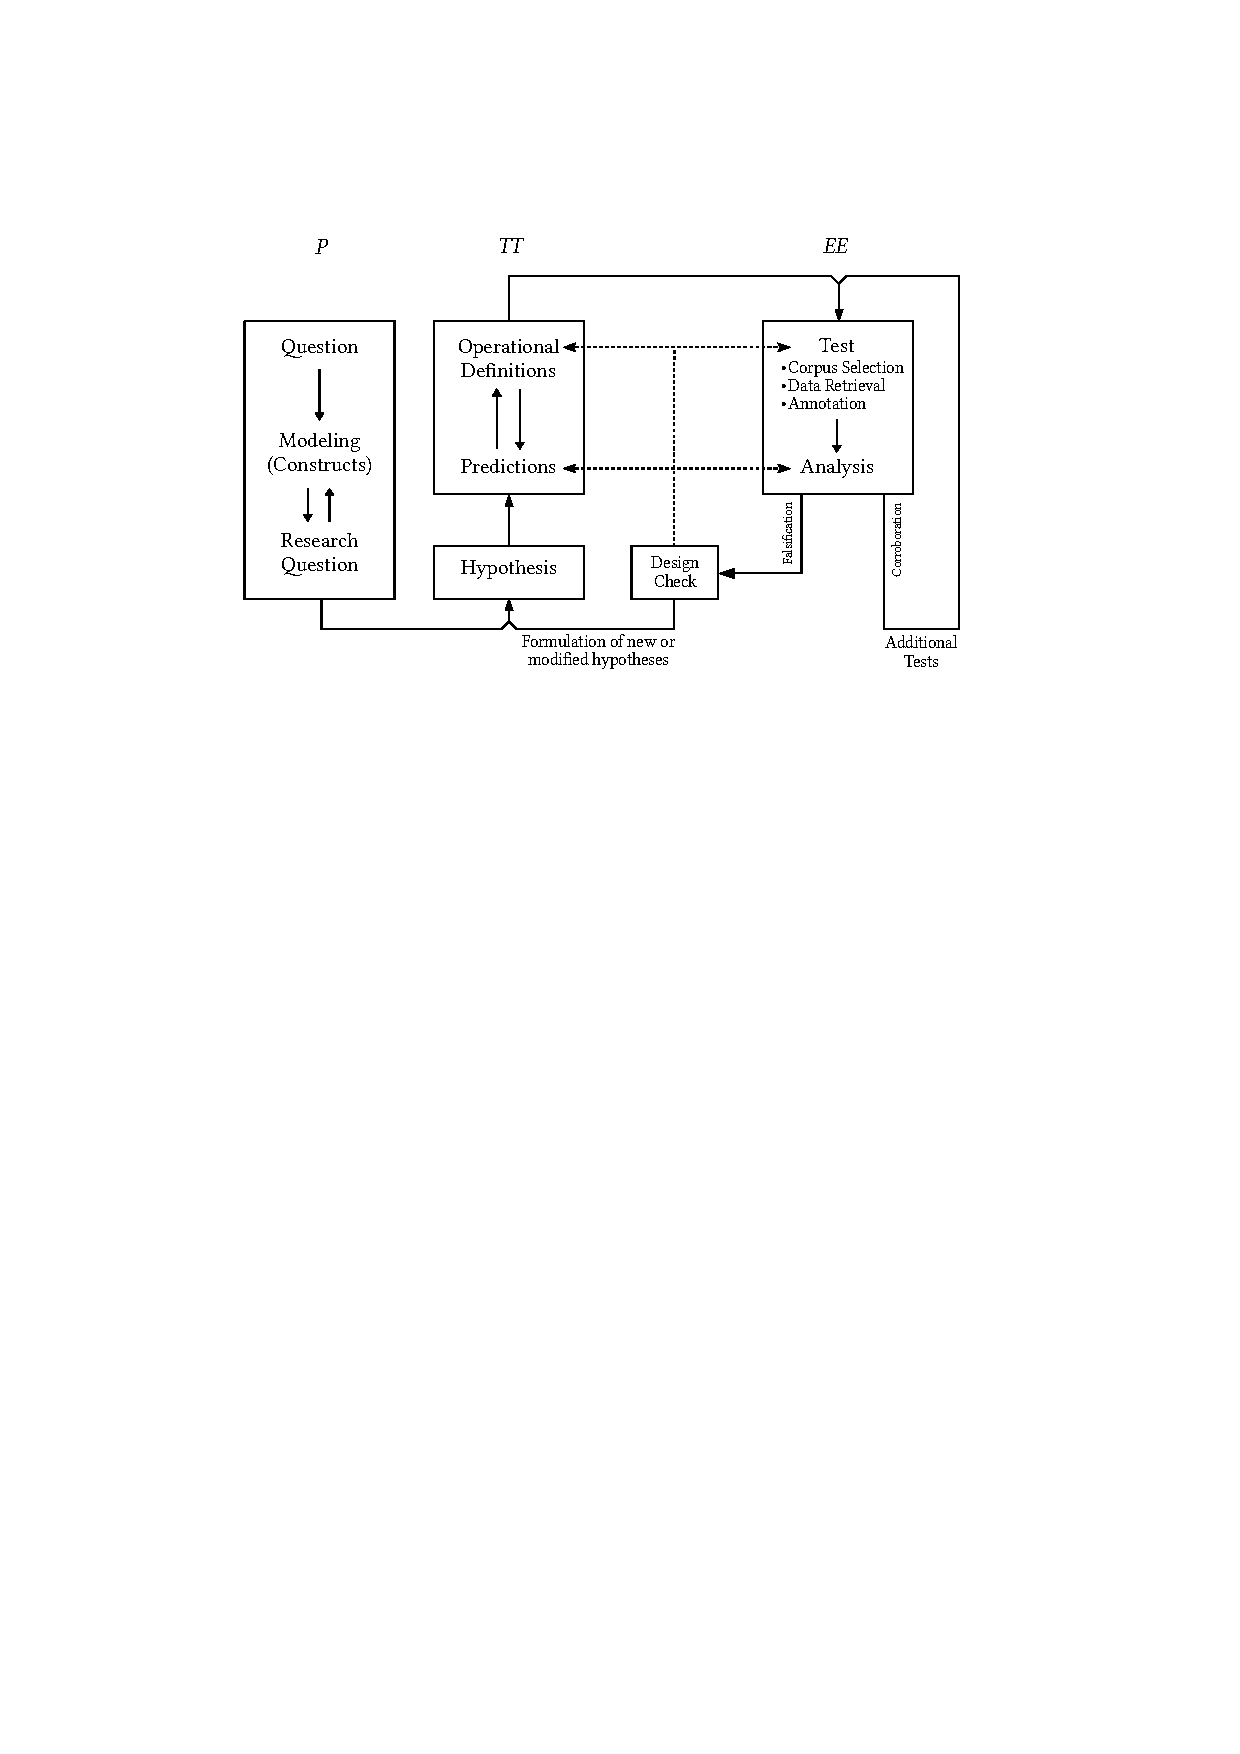
\includegraphics[scale=0.9]{figures/researchcycle}
\end{figure}

Research begins with a general question -- something that intrigues an individual or a group of researchers. The part of reality to which this question pertains is then modeled, i.e., described in terms of theoretical constructs, enabling us to formulate, first, a more specific research question, and often, second, a hypothesis. \is{hypothesis} There is nothing automatic about these steps -- they are typically characterized by lengthy critical discussion, false starts or wild speculation, until testable hypotheses emerge (in some disciplines, this stage has not yet been, and in some cases probably never will be reached). Next, predictions must be derived, requiring operational \is{operationalization} definitions of the constructs posited previously. This may require some back and forth between formulating predictions and providing sufficiently precise operationalizations.

Next, the predictions must be tested -- in the case of corpus linguistics, corpora must be selected and data must be retrieved \is{retrieval} and annotated, \is{annotation} something we will discuss in detail in the next chapter. Then the data are analyzed with respect to the hypothesis. \is{hypothesis} If they corroborate \is{corroboration} the hypothesis (or at least fail to falsify \is{falsification} it), this is not the end of the process: with Popper, we should only begin to accept evidence as corroborating when it emerges from repeated attempts to falsify the hypothesis. Thus, additional tests must be, and typically are, devised. If the results of any test falsify \is{falsification} the hypothesis, this does not, of course, lead to its immediate rejection. After all, we have typically arrived at our hypothesis based on good arguments, and so researchers will typically perform what we could call a ``design \is{research design} check'' on their experiment, \is{experimental method} looking closely at their predictions to see if they really follow from the hypothesis, \is{hypothesis} the operational \is{operationalization} definitions to see whether they are reliable \is{reliability} and valid \is{validity} with respect to the constructs they represent, and the test itself to determine whether there are errors or confounding variables in the data selection and analysis. If potential problems are found, they will be fixed and the test will be repeated. Only if it fails repeatedly will researchers abandon (or modify) the hypothesis.

The repeated testing, and especially the modification of a hypothesis \is{hypothesis} is inherently dangerous, as we might be so attached to our hypothesis that we will keep testing it long after we should have given it up, or that we will try to save it by changing it just enough that our test will no longer falsify \is{falsification} it, or by making it completely untestable \citep[cf.][37]{popper_conjectures_1963}. This must, of course, be avoided, but so must throwing out a hypothesis, \is{hypothesis} or an entire model, on the basis of a single falsification \is{falsification} event. Occasionally, especially in half\hyp{}mature disciplines like linguistics, models morph into competing schools of thought, each vigorously defended by its adherents even in the face of a growing number of phenomena that they fail to account for. In such cases, a radical break in the research cycles within these models may be necessary to make any headway at all -- a so\hyp{}called ``paradigm shifts'' occurs. This means that researchers abandon the current model wholesale and start from scratch based on different initial assumptions \citep[see][]{kuhn_structure_1962}. Corpus linguistics with its explicit recognition that generalizations about the language system can and must be deduced from language usage may present such a paradigm shift with respect to the intuition\hyp{}driven \is{intuition} generative \is{generative linguistics} models.

Finally, note that the scientific research cycle is not only incremental, with each new hypothesis \is{hypothesis} and each new test building on previous research, but that it is also collaborative, with one researcher or group of researchers picking up where another left off. This collaborative nature of research requires researchers to be maximally transparent with respect to their research designs, \is{research design} laying open their data and methods in sufficient detail for other researchers to understand exactly what prediction was tested, how the constructs in question were operationalized, \is{operationalization} how data were retrieved \is{retrieval} and analyzed. Again, this is the norm in disciplines like experimental \is{experimental method} physics and psychology, \is{psychology} but not so much so in the more humanities\hyp{}leaning \is{humanities} disciplines, which tend to put the focus on ideas and arguments rather than methods. We will deal with data retrieval and annotation \is{annotation} in the next chapter and return to the issue of methodological transparency at the end of it.


\chapter{Data retrieval and annotation}
\label{ch:retrievalannotation}


Traditionally, many corpus\hyp{}linguistic studies use the (orthographic) word form as their starting point. This is at least in part due to the fact that corpora consist of text that is represented as a sequence of word forms, and that, consequently, word forms are easy to retrieve. \is{retrieval} As briefly discussed in Chapter \ref{ch:corpuslinguistics}, concordancing \is{concordance} software allows us to query \is{query} the corpus for a string of characters and displays the result as a list of hits \is{hit} in context.

As we saw when discussing the case of \textit{pavement} in Chapter \ref{ch:scientificmethod}, a corpus query \is{query} for a string of characters like $\langle$ \texttt{pavement} $\rangle$ may give us more than we want -- it will return not only hits \is{hit} corresponding to the word sense ``pedestrian footpath'', which we could contrast with the synonym \is{synonymy} \textit{sidewalk}, but also those corresponding to the word sense ``hard surface'' (which we could contrast with the synonym \textit{paving}).

The query \is{query} may, at the same time, give us \emph{less} than we want, because it would only return the singular \is{number} form of the word and only if it is spelled entirely in lower case. A study of the word (in either or both of its senses) would obviously require that we look at the \emph{lemma} \is{lemma} PAVEMENT, comprising at least the word forms \textit{pavement} (singular), \textit{pavements} (plural) and, depending on how the corpus is prepared, \textit{pavement's} (possessive). It also requires that we include in our query \is{query} all possible graphemic variants, comprising at least cases in lower case, with an initial capital (\textit{Pavement, Pavements, Pavement's}, e.g. at the beginning of a sentence), or in all caps (\textit{PAVEMENT, PAVEMENTS, PAVEMENT'S)}, but, depending on the corpus, also hyphenated cases occurring at a line break (e.g. \textit{pave-}$\P$\textit{ment}, with $\P$ standing for the line break).

In Chapter \ref{ch:scientificmethod}, we implicitly treated the second issue as a problem of \textit{retrieval}, \is{retrieval} noting in passing that we queried \is{query} our corpus in such a way as to capture all variants of the lemma \is{lemma} PAVEMENT. We treated the first issue as a problem of categorization \is{categorization} -- we went through the results of our query one by one, determining from the context, which of the senses of \textit{pavement} we were likely dealing with. In the context of a research project, our decisions would be recorded together with the data in some way -- we would \emph{annotate} \is{annotation} the data, using an agreed\hyp{}upon \emph{code} \is{coding} for each of the categories \is{categorization} (e.g., word senses).

Retrieval is a non\hyp{}trivial issue even when dealing with individual lexical items whose orthographic representations are not ambiguous. \is{ambiguity} The more complex \is{complexity} the phenomena under investigation are, the more complex these issues become, requiring careful thought and a number of decisions concerning an almost inevitable trade\hyp{}off between the quality of the results and the time needed to retrieve \is{retrieval} them. This issue will be dealt with in Section \ref{sec:retrieval}. We already saw that the issue of data annotation \is{annotation} is extremely complex even in the case of individual lexical items, and the preceding chapter discussed some more complicated examples. This issue will be dealt with in more detail in Section \ref{sec:annotating}.

\section{Retrieval}
\label{sec:retrieval}

Broadly speaking, there are two ways of searching a corpus for a particular linguistic phenomenon: manually \is{manual analysis} (i.e., by reading the texts contained in it, noting down each instance of the phenomenon in question) or automatically (i.e., by using a computer program to run a query \is{query} on a machine\hyp{}readable version of the texts). As discussed in Chapter \ref{ch:corpuslinguistics}, there may be cases where there is no readily apparent alternative to a fully manual \is{manual analysis} search, and we will come back to such cases below.

However, as also discussed in Chapter \ref{ch:corpuslinguistics}, software\hyp{}aided queries \is{query} are the default in modern corpus linguistics, and so we take these as a starting point of our discussion.

\subsection{Corpus queries}
\label{sec:corpusqueries}

There is a range of more or less specialized commercial and non\hyp{}commercial concordancing \is{concordance} programs designed specifically for corpus linguistic research, and there are many other software packages that may be repurposed to the task of searching text corpora even though they are not specifically designed for corpus\hyp{}linguistic research. Finally, there are scripting languages like Perl, Python and R, with a learning curve that is not forbiddingly steep, that can be used to write programs capable of searching text corpora (ranging from very simple two\hyp{}liners to very complex solutions). Which of these solutions are available to you and suitable to your research project is not for me to say, so the following discussion will largely abstract away from such specifics.

The power of software\hyp{}aided searches depends on two things: first, on the annotation \is{annotation} contained in the corpus itself and second, on the pattern\hyp{}matching capacities of the software used to access them. In the simplest case (which we assumed to hold in the examples discussed in the previous chapter), a corpus will contain plain text in a standard orthography and the software will be able to find passages matching a specific string of characters. Essentially, this is something every word processor is capable of.

Most concordancing \is{concordance} programs can do more than this, however. For example, they typically allow the researcher to formulate queries \is{query} that match not just one string, but a class of strings. One fairly standardized way of achieving this is by using so\hyp{}called ``regular expressions'' -- strings that may contain not just simple characters, but also symbols referring to classes of characters or symbols affecting the interpretation of characters. For example, the lexeme \textit{sidewalk}, has (at least) six possible orthographic representations: \textit{sidewalk}, \textit{side-walk}, \textit{Sidewalk}, \textit{Side-walk}, \textit{sidewalks}, \textit{side-walks}, \textit{Sidewalks} and \textit{Side-walks} (in older texts, it is sometimes spelled as two separate words, which means that we have to add at least \textit{side walk}, \textit{side walks}, \textit{Side walk} and \textit{Side walks} when investigating such texts). In order to retrieve \is{retrieval} all occurrences of the lexeme, we could perform a separate query \is{query} for each of these strings, but I actually queried the string in (\ref{ex:regexexample}a); a second example of regular expressions is (\ref{ex:regexexample}b), which represents one way of searching for all inflected forms and spelling variants of the verb \is{verb} \textit{synthesize} (as long as they are in lower case):

\begin{exe}
\ex
\begin{xlist}
\label{ex:regexexample}
\ex \texttt{[Ss]ide[- ]?walks?}
\ex \texttt{synthesi[sz]e?[ds]?(ing)?}
\end{xlist}
\end{exe}

Any group of characters in square brackets is treated as a class, which means that any one of them will be treated as a match, and the question mark means ``zero or one of the preceding characters''. This means that the pattern in (\ref{ex:regexexample}a) will match an upper- or lower\hyp{}case \textit{S}, followed by \textit{i}, \textit{d}, and \textit{e}, followed by zero or one occurrence of a hyphen or a blank space, followed by \textit{w}, \textit{a}, \textit{l}, and \textit{k}, followed by zero or one occurrence of \textit{s}. This matches all the variants of the word. For (\ref{ex:regexexample}b), the [sz] ensures that both the British \is{British English} spelling (with an \textit{s}) and the American \is{American English} spelling (with a \textit{z}) are found. The question mark after \textit{e} ensures that both the forms with an \textit{e} (\textit{synthesize, synthesizes, synthesized}) and that without one (\textit{synthesizing}) are matched. Next, the string matches zero to one occurrence of a \textit{d} or an \textit{s} followed by zero or one occurrence of the string \textit{ing} (because it is enclosed in parentheses, it is treated as a unit for the purposes of the following question mark.

Regular expressions allow us to formulate the kind of complex and abstract queries \is{query} that we are likely to need when searching for words (rather than individual word forms) and even more so when searching for more complex expressions. But even the simple example in (\ref{ex:regexexample}) demonstrates a problem with such queries: they quickly overgeneralize. The pattern would also, for example, match some non\hyp{}existing forms, like \textit{synthesizding}, and, more crucially, it will match existing forms that we may not want to include in our search results, like the noun \is{noun} \textit{synthesis} (see further Section \ref{sec:precisionrecall}).

The benefits of being able to define complex queries \is{query} become even more obvious if our corpus contains annotations \is{annotation} in addition to the original text, as discussed in Section \ref{sec:annotations} of Chapter \ref{ch:corpuslinguistics}. If the corpus contains part\hyp{}of\hyp{}speech tags, for example, this will allow us to search (within limits) for grammatical structures. For example, assume that there is a part\hyp{}of\hyp{}speech tag \is{POS tagging} attached to the end of every word by an underscore (as in the BROWN \is{BROWN} corpus, see example (\ref{fig:brownstructfeatures}) in Chapter \ref{ch:corpuslinguistics}) and that the tags are as shown in (\ref{ex:browntags}) (following the sometimes rather nontransparent BROWN \is{BROWN} naming conventions). We could then search for prepositional \is{adposition} phrases using a pattern like the one in (\ref{ex:npqueryregex}): \is{query}

\begin{exe}
\ex
\begin{tabular}[t]{ll}
preposition & \texttt{\_IN}\\
articles & \texttt{\_AT}\\
adjectives & \texttt{\_JJ} (uninflected)\\
 & \texttt{\_JJR} (comparative)\\
 & \texttt{\_JJT} (superlative)\\
nouns & \texttt{\_NN} (common singular nouns)\\
 & \texttt{\_NNS} (common plural nouns)\\
 & \texttt{\_NN\$} (common nouns with possessive clitic)\\
 & \texttt{\_NP} (proper names)\\
 & \texttt{\_NP\$} (proper nouns with possessive clitic) \is{clitic}
\end{tabular}
\label{ex:browntags}
\end{exe}

\begin{exe}
\ex
\begin{tabular}[t]{cccc}
\texttt{\textbackslash{}S+\_IN} & \texttt{(\textbackslash{}S+\_AT)?} & \texttt{(\textbackslash{}S+\_JJ[RT]?)*} & \texttt{(\textbackslash{}S+\_N[PN][S\$]?)+}\\
1 & 2 & 3 & 4
\end{tabular}
\label{ex:npqueryregex}
\end{exe}

An asterisk means ``zero or more'', a plus means ``one or more'', and \textbackslash{}S means ``any non\hyp{}whitespace character'', the meaning of the other symbols is as before. The pattern in (\ref{ex:npqueryregex}) \is{query} matches the following sequence:

\begin{enumerate}
\item any word (i.e., sequence of non\hyp{}whitespace characters) tagged \is{POS tagging} as a preposition, \is{adposition} followed by
\item zero or one occurrence of a word tagged as an article \is{determiner} that is preceded by a whitespace, followed by
\item zero or more occurrences of a word tagged as an adjective \is{adjective} (again preceded by a whitespace), including comparatives and superlatives -- note that the JJ tag may be followed by zero or one occurrence of a \textit{T} or an \textit{R}), followed by
\item one or more words (again, preceded by a whitespace) that are tagged \is{POS tagging} as a noun \is{noun} or proper name (note the square bracket containing the N for common nouns and the P for proper nouns), including plural \is{number} forms and possessive forms (note that NN or NP tags may be followed by zero or one occurrence of an S or a \$).
\end{enumerate}

The query \is{query} in (\ref{ex:npqueryregex}) makes use of the annotation \is{annotation} in the corpus (in this case, the part\hyp{}of\hyp{}speech tagging), \is{POS tagging} but it does so in a somewhat cumbersome way by treating word forms and the tags attached to them as strings. As shown in Figure \ref{fig:susanneannotation} in Chapter \ref{ch:corpuslinguistics}, corpora often contain multiple annotations \is{annotation} for each word form -- part of speech, lemma, \is{lemma} in some cases even grammatical structure. Some concordance \is{concordance} programs, such as the widely\hyp{}used open\hyp{}source Corpus Workbench (including its web\hyp{}based version CQPweb) \citep[cf.][]{evert_twenty-first_2011} or the Sketch Engine and its open\hyp{}source variant NoSketch engine \citep[cf.][]{kilgarriff_sketch_2014} are able to ``understand'' the structure of such annotations \is{annotation} and offer a query \is{query} syntax that allows the researcher to refer to this structure directly.

The two programs just mentioned share a query \is{query} syntax called \emph{CQP} (for ``Corpus Query Processor'') in the Corpus Workbench and \emph{CQL} (for ``Corpus Query Language'') in the (No)Sketch Engine. This syntax is very powerful, allowing us to query the corpus for tokens or sequences of tokens at any level of annotation. \is{annotation} It is also very transparent: each token is represented as a value\hyp{}attribute pair in square brackets, as shown in (\ref{ex:cqptoken}):

\begin{exe}
\ex \texttt{[attribute="value"]}
\label{ex:cqptoken}
\end{exe}

The attribute refers to the level of annotation \is{annotation} (e.g. \texttt{word}, \texttt{pos}, \texttt{lemma} \is{lemma} or whatever else the makers of a corpus have called their annotations), the value refers to what we are looking for. For example, a query \is{query} for the different forms of the word \textit{synthesize} (cf. (\ref{ex:regexexample}) above) would look as shown in (\ref{ex:cqpexample}a), or, if the corpus contains information about the lemma of each word form, as shown in (\ref{ex:cqpexample}b), and the query for PPs in (\ref{ex:npqueryregex}) would look as shown in (\ref{ex:cqpexample}c):

\begin{exe}
\ex
\begin{xlist}
\label{ex:cqpexample}
\ex \texttt{[word="synthesi[sz]e?[ds]?(ing)?"]}
\ex \texttt{[lemma="synthesize"]}
\ex \texttt{[pos="IN"]} \texttt{[pos="AT"]?} \texttt{[pos="JJ[RT]"]\*} \texttt{[pos="N[PN][S\$]?"]+}
\end{xlist}
\end{exe}

As you can see, we can use regular expressions inside the values for the attributes, and we can use the asterisk, question mark and plus outside the token to indicate that the query \is{query} should match ``zero or more'', ``zero or one'' and ``one or more'' tokens with the specified properties. Note that CQP syntax is case sensitive, so for example (\ref{ex:cqpexample}a) would only return hits \is{hit} that are in lower case. If we want the query to be case\hyp{}insensitive, we have to attach \texttt{\%c} to the relevant values.

We can also combine two or more attribute\hyp{}value pairs inside a pair of square brackets to search for tokens satisfying particular conditions at different levels of annotation. \is{annotation} For example, (\ref{ex:cqpmoreexample}a) will find all instances of the word form \textit{walk} tagged \is{POS tagging} as a verb, \is{verb} while (\ref{ex:cqpmoreexample}b) will find all instances tagged as a noun. \is{noun} We can also address different levels of annotation at different positions in a query. \is{query} For example, (\ref{ex:cqpmoreexample}c) will find all instances of the word form \textit{walk} followed by a word tagged \is{POS tagging} as a preposition, \is{adposition} and (\ref{ex:cqpmoreexample}d) corresponds to the query $\langle$ \texttt{through the NOUN of POSS.PRON car} $\rangle$ mentioned in Section \ref{sec:statinghypotheses} of Chapter \ref{ch:scientificmethod} (note the \texttt{\%c} that makes all queries \is{query} for words case\hyp{}insensitive):


\begin{exe}
\ex
\begin{xlist}
\label{ex:cqpmoreexample}
\ex \texttt{[word="walk"\%c \& pos="VB"]}
\ex \texttt{[word="walk"\%c \& pos="NN"]}
\ex \texttt{[word="walk"\%c]} \texttt{[pos="IN"]}
\ex \begin{minipage}[t]{0.85\textwidth} \raggedright \texttt{[word="through"\%c]} \texttt{[word="the"\%c]} \texttt{[pos="NNS?"]} \texttt{[word="of"\%c]} \texttt{[pos="PP\$"]} \texttt{[word="car"\%c]} \end{minipage}
\end{xlist}
\end{exe}

This query syntax is so transparent and widely used that we will treat it as a standard in the remainder of the book and use it to describe queries. This is obviously useful if you are using one of the systems mentioned above, but if not, the transparency of the syntax should allow you to translate the query \is{query} into whatever possibilities your concordancer \is{concordance} offers you. When talking about a query in a particular corpus, I will use the annotation \is{annotation} (e.g., the part\hyp{}of\hyp{}speech tags) used in that corpus, when talking about queries in general, I will use generic values like \textit{noun} \is{noun} or \textit{prep.}, shown in lower case to indicate that they do not correspond to a particular corpus annotation.

Of course, even the most powerful query syntax can only work with what is there. Retrieving instances of phrasal categories based on part\hyp{}of\hyp{}speech annotation \is{annotation} is only possible to a certain extent: even a complex query like that in (\ref{ex:cqpexample}c) or in (\ref{ex:npqueryregex}) will not return all prepositional \is{adposition} phrases. These queries \is{query} will not, for example, match cases where the adjective \is{adjective} is preceded by one or more quantifiers (tagged \is{POS tagging} \texttt{\_QT} in the BROWN \is{BROWN} corpus), adverbs \is{adverb} (tagged \texttt{\_RB}), or combinations of the two. It will also not return cases with pronouns \is{pronoun} instead of nouns. \is{noun} These and other issues can be fixed by augmenting the query accordingly, although the increasing complexity will bring problems of its own, to which we will return in the next subsection.

Other problems are impossible to fix; for example, if the noun \is{noun} phrase inside the PP contains another PP, the pattern will not recognize it as belonging to the NP but will treat it as a new match and there is nothing we can do about this, since there is no difference between the sequence of POS tags in a structures like (\ref{ex:ppattachment}a), where the PP \textit{off the kitchen} is a complement of the noun \textit{room} and as such is part of the NP inside the first PP, and (\ref{ex:ppattachment}b), where the PP \textit{at a party} is an adjunct of the verb \is{verb} \textit{standing} and as such is not part of the NP preceding it:

\begin{exe}
\ex
\begin{xlist}
\label{ex:ppattachment}
\ex A mill stands \textit{in a room off the kitchen}. (BROWN F04)
\ex He remembered the first time he saw her, standing \textit{across the room at a party}. (BROWN P28)
\end{xlist}
\end{exe}

In order to distinguish these cases in a query, \is{query} we need a corpus annotated \is{annotation} not just for parts of speech but also for syntactic \is{syntax} structure (sometimes referred to as a \textit{treebank}), like the SUSANNE corpus briefly discussed in Section \ref{sec:annotations} of Chapter \ref{ch:corpuslinguistics} above.


\subsection{Precision and recall}
\label{sec:precisionrecall}

In arriving at the definition of corpus linguistics adopted in this book, we stressed the need to investigate linguistic phenomena exhaustively, which we took to mean ``taking into account all examples of the phenomenon in question'' (cf. Chapter \ref{ch:corpuslinguistics}). In order to take into account all examples of a phenomenon, we have to retrieve \is{retrieval} them first. However, as we saw in the preceding section and in Chapter \ref{ch:scientificmethod}, it is not always possible to define a corpus query \is{query} in a way that will retrieve all and only the occurrences of a particular phenomenon. Instead, a query can have four possible outcomes: it may

\begin{enumerate}
\item include hits \is{hit} that are instances of the phenomenon we are looking for (these are referred to as a \textit{true positives} or \textit{hits}, but note that we are using the word \textit{hit} in a broader sense to mean ``anything returned as a result of a query''); \is{query}
\item include hits \is{hit} that are not instances of our phenomenon (these are referred to as a \textit{false positives});
\item fail to include instances of our phenomenon (these are referred to as a \textit{false negatives} or \textit{misses}); or
\item fail to include strings that are not instances of our phenomenon (this is referred to as a \textit{true negative}).
\end{enumerate}

Table \ref{tab:queryoutcomes} summarizes these outcomes ($\lnot$ stands for ``not'').

\begin{table}[!htbp]
\caption{Four possible outcomes of a corpus query for a given phenomenon X}
\label{tab:queryoutcomes}
\begin{tabular}[t]{lrcc}
\lsptoprule
 & & \multicolumn{2}{c}{Search result} \\
 & & Included & Not included \\
\midrule
Corpus & X & \makecell[t]{True positive \\ \footnotesize{(\textit{hit})}} & \makecell[t]{False negative \\ \footnotesize{(\textit{miss})}} \\
 & $\lnot$ X & \makecell[t]{False positive \\ \footnotesize{(\textit{false alarm})}} & \makecell[t]{True negative \\ \footnotesize{(\textit{correct rejection})}} \\
\lspbottomrule
\end{tabular}
\end{table}

Obviously, the first case (true positive) and the fourth case (true negative) are desirable outcomes: we want our search results to include all instances of the phenomenon under investigation and exclude everything that is not such an instance. The second case (false negative) and the third case (false positive) are undesirable outcomes: we do not want our query \is{query} to miss instances of the phenomenon in question and we do not want our search results to incorrectly include strings that are not instances of it.

We can describe the quality of a data set that we have retrieved \is{retrieval} from a corpus in terms of two measures. First, the proportion of positives (i.e., strings returned by our query) \is{query} that are true positives; this is referred to as \textit{precision}, \is{precision} or as the \textit{positive predictive value}, cf. (\ref{ex:precisionrecall}a). Second, the proportion of all instances of our phenomenon that are true positives (i.e., that were actually returned by our query; this is referred to as \textit{recall}, \is{recall} cf. (\ref{ex:precisionrecall}b):\footnote{There are two additional measures that are important in other areas of empirical research but do not play a central role in corpus\hyp{}linguistic data retrieval. \is{retrieval} First, the \emph{specificity} or true negative rate -- the proportion of negatives that are incorrectly included in our data (i.e. false negatives); second, \emph{negative predictive value} -- the proportion of negatives (i.e., cases not included in our search) that are true negatives (i.e., that are correctly rejected). These measures play a role in situations where a negative outcome of a test is relevant (for example, with medical diagnoses); in corpus linguistics, this is generally not the case. There are also various scores that combine individual measures to give us an overall idea of the accuracy of a test, for example, the \emph{F1 score}, defined as the harmonic mean of precision \is{precision} and recall. \is{recall} Such scores are useful in information retrieval \is{retrieval} or machine learning, but less so in corpus\hyp{}linguistic research projects, where precision and recall must typically be assessed independently of, and weighed against, each other.}

\begin{exe}
\ex
\begin{xlist}
\label{ex:precisionrecall}
\ex $\displaystyle{\text{Precision} = \frac{\text{True Positives}}{\text{True Positives} + \text{False Positives}}}$\\
\ex $\displaystyle{\text{Recall} = \frac{\text{True Positives}}{\text{True Positives} + \text{False Negatives}}}$
\end{xlist}
\end{exe}

Ideally, the value of both measures should be 1, i.e., our data should include all cases of the phenomenon under investigation (a recall \is{recall} rate of 100 percent) and it should include nothing that is not a case of this phenomenon (a precision \is{precision} of 100 percent). However, unless we carefully search our corpus manually \is{manual analysis} (a possibility I will return to below), there is typically a trade\hyp{}off between the two. Either we devise a query \is{query} that matches only clear cases of the phenomenon we are interested in (high precision) but that will miss many less clear cases (low recall). \is{recall} Or we devise a query that matches as many potential cases as possible (high recall), but that will include many cases that are not instances of our phenomenon (low precision). \is{precision}

Let us look at a specific example, the English ditransitive \is{ditransitivity} construction, and let us assume that we have an untagged \is{POS tagging} and unparsed corpus. How could we retrieve \is{retrieval} instances of the ditransitive? As the first object of a ditransitive is usually a pronoun \is{pronoun} (in the objective case) and the second a lexical NP (see, for example, \citealt{thompson_iconicity_1987}), one possibility would be to search for a pronoun \is{pronoun} followed by a determiner \is{determiner} (i.e., for any member of the set of strings in (\ref{ex:ditransitivequery}a)), followed by any member of the set of strings in (\ref{ex:ditransitivequery}b)). \is{ditransitivity} This gives us the query \is{query} in (\ref{ex:ditransitivequery}c), which is long, but not very complex:

\begin{exe}
\ex
\begin{xlist}
\label{ex:ditransitivequery}
\ex \textit{me}, \textit{you}, \textit{him}, \textit{her}, \textit{it}, \textit{us}, \textit{them}
\ex \textit{the}, \textit{a}, \textit{an}, \textit{this}, \textit{that}, \textit{these}, \textit{those}, \textit{some}, \textit{many}, \textit{lots}, \textit{my}, \textit{your}, \textit{his}, \textit{her}, \textit{its}, \textit{our}, \textit{their}, \textit{something}, \textit{anything}
\ex \begin{minipage}[t]{0.85\textwidth} \raggedright \texttt{[word="(me|\allowbreak you|\allowbreak him|\allowbreak her|\allowbreak it|\allowbreak us|\allowbreak them)"\%c]} \texttt{[word="(the|\allowbreak a|\allowbreak an|\allowbreak this|\allowbreak that|\allowbreak these|\allowbreak those|\allowbreak some|\allowbreak many|\allowbreak lots|\allowbreak my|\allowbreak your|\allowbreak his|\allowbreak her|\allowbreak its|\allowbreak our|\allowbreak their|\allowbreak something|\allowbreak anything)"\%c]} \end{minipage}
\end{xlist}
\end{exe}

Let us apply this query \is{query} (which is actually used in \citealt{colleman_constructional_2011}) to a freely available sample from the British Component of the International Corpus of English mentioned in Chapter \ref{ch:corpuslinguistics} above (see the Study Notes to the current chapter for details). This corpus has been manually annotated, \is{annotation} amongst other things, for argument structure, so that we can check the results of our query \is{query} against this annotation. \is{annotation}

There are 36 ditransitive \is{ditransitivity} clauses in the sample, thirteen of which are returned by our query. \is{query} There are also 2838 clauses that are not ditransitive, 14 of which are also returned by our query. Table \ref{tab:queryoutcomesexample} shows the results of the query in terms of true and false positives and negatives:

\begin{table}[!htbp]
\caption{Comparison of the search results}
\label{tab:queryoutcomesexample}
\begin{tabular}[t]{lrccr}
\lsptoprule
 & & \multicolumn{2}{c}{Search result} & \\
 & & Included & Not included & Total \\
\midrule
Corpus & Ditransitive & \makecell[t]{13 \\ \footnotesize{\textit{true positives}}} & \makecell[t]{23 \\ \footnotesize{\textit{false negatives}}} & 36 \\
 & $\lnot$ Ditransitive & \makecell[t]{14 \\ \footnotesize{\textit{false positives}}} & \makecell[t]{2824 \\ \footnotesize{\textit{true negatives}}} & 2838 \\
\midrule
 & Total & 27 & 2847 & 2874 \\
\lspbottomrule
\end{tabular}
\end{table}

We can now calculate precision \is{precision} and recall \is{recall} rate of our query: \is{query}

\begin{exe}
\ex
\begin{xlist}
\label{ex:precisionrecallrate}
\ex $\displaystyle{Precision = \frac{13}{27} = 0.48}$\\
\ex $\displaystyle{Recall = \frac{13}{36} = 0.36}$
\end{xlist}
\end{exe}

Clearly, neither precision \is{precision} nor recall \is{recall} are particularly impressive. Let us look at the reasons for this, beginning with precision.

While the sequence of a pronoun \is{pronoun} and a determiner \is{determiner} is typical for (one type of) ditransitive \is{ditransitivity} clause, it is not unique to the ditransitive, as the following false positives of our query \is{query} show:

\begin{exe}
\ex
\begin{xlist}
\label{ex:ditrfalsepositives}
\ex ... one of the experiences that went towards making me a Christian...
\ex I still ring her a lot.
\ex I told her that I'd had to take these tablets
\ex It seems to me that they they tend to come from
\ex Do you need your caffeine fix before you this
\end{xlist}
\end{exe}

Two other typical structures characterized by the sequence pronoun\hyp{}determiner \is{pronoun} \is{determiner} are object\hyp{}complement \is{complementation} clauses (cf. (\ref{ex:ditrfalsepositives}a)) and clauses with quantifying noun \is{noun} phrases (cf. (\ref{ex:ditrfalsepositives}b)). In addition, some of the strings in (\ref{ex:ditransitivequery}b) above are ambiguous, \is{ambiguity} i.e., they can represent parts of speech other than determiner; \is{determiner} for example, \textit{that} can be a conjunction, \is{conjunction} as in (\ref{ex:ditransitivequery}c), \is{query} which otherwise fits the description of a ditransitive, \is{ditransitivity} and in (\ref{ex:ditrfalsepositives}d), which does not. Finally, especially in spoken \is{medium} corpora, there may be fragments that match particular search criteria only accidentally (cf. (\ref{ex:ditrfalsepositives}e)). Obviously, a corpus tagged \is{POS tagging} for parts of speech could improve the precision \is{precision} of our search results somewhat, by excluding cases like (\ref{ex:ditransitivequery}c-d), but others, like (\ref{ex:ditransitivequery}a), could never be excluded, since they are identical to the ditransitive as far as the sequence of parts\hyp{}of\hyp{}speech is concerned.

Of course, it is relatively trivial, in principle, to increase the precision \is{precision} of our search results: we can manually \is{manual analysis} discard all false positives, which would increase precision to the maximum value of 1. Typically, our data will have to be manually annotated \is{annotation} for various criteria anyway, allowing us to discard false positives in the process. However, the larger \is{corpus size} our data set, the more time consuming this will become, so precision \is{precision} should always be a consideration even at the stage of data retrieval. \is{retrieval}

Let us now look at the reasons for the recall \is{recall} rate, which is even worse than the precision. \is{precision} There are, roughly speaking, four types of ditransitive \is{ditransitivity} structures that our query \is{query} misses, exemplified in (\ref{ex:ditrfalsenegatives}a--e):

\begin{exe}
\ex
\begin{xlist}
\label{ex:ditrfalsenegatives}
\ex How much money have they given you?
\ex The centre [...] has also been granted a three\hyp{}year repayment freeze.
\ex He gave the young couple his blessing.
\ex They have just given me enough to last this year.
\ex He finds himself [...] offering Gradiva flowers.
\end{xlist}
\end{exe}

The first group of cases are those where the second object does not appear in its canonical position, for example in interrogatives and other cases of left\hyp{}dislocation (cf. \ref{ex:ditrfalsenegatives}a), or passives \is{passive voice} (\ref{ex:ditrfalsenegatives}b). The second group of cases are those where word order \is{order} is canonical, but either the first object (\ref{ex:ditrfalsenegatives}c) or the second object (\ref{ex:ditrfalsenegatives}d) or both (\ref{ex:ditrfalsenegatives}e) do not correspond to the query. \is{query}

Note that, unlike precision, \is{precision} the recall \is{recall} rate of a query \is{query} cannot be increased after the data have been extracted \is{retrieval} from the corpus. Thus, an important aspect in constructing a query is to annotate \is{annotation} a random sample \is{sampling} of our corpus manual \is{manual analysis} for the phenomenon we are interested in, and then to check our query against this manual annotation. \is{annotation} This will not only tell us how good or bad the recall of our query is, it will also provide information about the most frequent cases we are missing. Once we know this, we can try to revise our query \is{query} to take these cases into account. In a POS\hyp{}tagged \is{POS tagging} corpus, we could, for example, search for a sequence of a pronoun \is{pronoun} and a noun \is{noun} in addition to the sequence pronoun\hyp{}determiner \is{determiner} that we used above, which would give us cases like (\ref{ex:ditrfalsenegatives}d), or we could search for forms of \textit{be} followed by a past participle followed by a determiner or noun, which would give us passives \is{passive voice} like those in (\ref{ex:ditrfalsenegatives}b).

In some cases, however, there may not be any additional patterns that we can reasonably search for. In the present example with an untagged \is{POS tagging} corpus, for example, there is no additional pattern that seems in any way promising. In such cases, we have two options for dealing with low recall: \is{recall} First, we can check (in our manually \is{manual analysis} annotated \is{annotation} subcorpus) whether the data that were recalled differ from the data that were not recalled in any way that is relevant for our research question. If this is not the case, we might decide to continue working with a low recall and hope that our results are still generalizable -- \citet{colleman_constructional_2011}, for example, are mainly interested in the question which classes of verbs \is{verb} were used ditransitively \is{ditransitivity} at what time in the history of English, a question that they were able to discuss insightfully based on the subset of ditransitives matching their query. \is{query}

If our data \textit{do} differ along one or more of the dimensions relevant to our research project, we might have to increase the recall \is{recall} at the expense of precision \is{precision} and spend more time weeding out false positives. In the most extreme case, this might entail extracting \is{retrieval} the data manually, \is{manual analysis} so let us return to this possibility in light of the current example.

\subsection{Manual, semi\hyp{}manual and automatic searches}
\label{sec:searchtypes}

In theory, the highest quality search results would always be achieved by a kind of close reading, i.e. a careful word\hyp{}by\hyp{}word (or phrase\hyp{}by\hyp{}phrase, clause\hyp{}by\hyp{}clause) inspection of the corpus. \is{manual analysis} As already discussed in Chapter \ref{ch:corpuslinguistics}, this may sometimes be the only feasible option, either because automatic retrieval \is{retrieval} is difficult (as in the case of searching for ditransitives \is{ditransitivity} in an untagged \is{POS tagging} corpus), or because an automatic retrieval is impossible (e.g., because the phenomenon we are interested in does not have any consistent formal properties, a point we will return to presently).

As discussed above, in the case of words and in at least some cases of grammatical structures, the quality of automatic searches may be increased by using a corpus annotated \is{annotation} automatically with part\hyp{}of\hyp{}speech tags, phrase tags or even grammatical structures. As discussed in Section \ref{sec:partsofspeech} of Chapter \ref{ch:scientificmethod}, this brings with it its own problems, as automatic tagging \is{POS tagging} and grammatical parsing are far from perfect. Still, an automatically annotated \is{annotation} corpus will frequently allow us to define searches whose precision \is{precision} and recall \is{recall} are higher than in the example above.

In the case of many other phenomena, however, automatic annotation \is{annotation} is simply not possible, or yields a quality so low that it simply does not make sense to base queries \is{query} on it. For example, linguistic metaphors \is{figurative language} \is{metaphor} are almost impossible to identify automatically, as they have little or no properties that systematically set them apart from literal \is{literalness} language. Consider the following examples of the metaphors \textsc{anger \is{emotions} is heat} and \textsc{anger is a (hot) liquid} (from \citealt[203]{lakoff_cognitive_1987}):

\begin{exe}
\ex
\begin{xlist}
\label{ex:angerheatnonpattern}
\ex Boy, am I burned up.
\ex He's just letting off steam.
\ex I had reached the boiling point.
\end{xlist}
\end{exe}

The first problem is that while the expressions in (\ref{ex:angerheatnonpattern}a-c) may refer to feelings \is{emotions} of anger or rage, they can also occur in their literal \is{literalness} meaning, as the corresponding authentic \is{authenticity} examples in (\ref{ex:literalheatnopattern}a--c) show:

\begin{exe}
\ex
\begin{xlist}
\label{ex:literalheatnopattern}
\ex ``Now, after I am burned up,'' he said, snatching my wrist, ``and the fire is out, you \textit{must} scatter the ashes. ..." (Anne Rice, \textit{The Vampire Lestat})
\ex As soon as the driver saw the train which had been hidden by the curve, he let off steam and checked the engine... (Galignani, \textit{Accident on the Paris and Orleans Railway})
\ex Heat water in saucepan on highest setting until you reach the boiling point and it starts to boil gently. (www.sugarfreestevia.net)
\end{xlist}
\end{exe}

Obviously, there is no query \is{query} that would find the examples in (\ref{ex:angerheatnonpattern}) \is{emotions} but not those in (\ref{ex:literalheatnopattern}). In contrast, it is very easy for a human to recognize the examples in (\ref{ex:literalheatnopattern}) as literal. \is{literalness} If we are explicitly interested in metaphors \is{figurative language} \is{metaphor} involving liquids and\slash or heat, we could choose a semi\hyp{}manual \is{manual analysis} approach, first extracting \is{retrieval} all instances of words from the field of liquids and\slash or heat and then discarding all cases that are not metaphorical. This kind of approach is used quite fruitfully, for example, by \citet{deignan_metaphor_2005}, amongst others.

If we are interested in metaphors \is{figurative language} \is{metaphor} of anger \is{emotions} in general, however, this approach will not work, since we have no way of knowing beforehand which semantic \is{semantics} fields to include in our query. \is{query} This is precisely the situation where exhaustive retrieval \is{retrieval} can only be achieved by a manual \is{manual analysis} corpus search, i.e., by reading the entire corpus and deciding for each word, phrase or clause, whether it constitutes an example of the phenomenon we are looking for. Thus, it is not surprising that many corpus\hyp{}linguistic studies on metaphor \is{figurative language} \is{metaphor} are based on manual searches (see, for example, \citet{semino_politics_1996} or \citet{jakel_metaphern_1997} for very thorough early studies of this kind).

However, as mentioned in Chapter \ref{ch:corpuslinguistics}, manual \is{manual analysis} searches are very time\hyp{}consuming and this limits their practical applicability: either we search large \is{corpus size} corpora, in which case manual searching is going to take more time and human resources than are realistically available, or we perform the search in a realistic time\hyp{}frame and with the human resources realistically available, in which case we have to limit the size \is{corpus size} of our corpus so severely that the search results can no longer be considered representative \is{representativeness} of the language as a whole. Thus, manual \is{manual analysis} searches are useful mainly in the context of research projects looking at a linguistic phenomenon in some clearly defined subtype of language (for example, metaphor \is{figurative language} \is{metaphor} in political speeches, see \citet{charteris-black_politicians_2005}).

When searching corpora for such hard\hyp{}to\hyp{}retrieve \is{retrieval} phenomena, it may sometimes be possible to limit the analysis usefully to a subset of the available data, as shown in the previous subsection, where limiting the query \is{query} for the ditransitive \is{ditransitivity} to active declarative clauses with canonical word order \is{order} still yielded potentially useful results. It depends on the phenomenon and the imagination of the researcher to find such easier\hyp{}to\hyp{}retrieve subsets.

To take up the example of metaphors \is{figurative language} \is{metaphor} introduced above, consider the examples in (\ref{ex:angerheatpattern}), \is{emotions} which are quite close in meaning to the corresponding examples in (\ref{ex:angerheatnonpattern}a--c) above (also from \citealt[189, 203]{lakoff_cognitive_1987}):

\begin{exe}
\ex
\begin{xlist}
\label{ex:angerheatpattern}
\ex He was consumed by his anger.
\ex He was filled with anger.
\ex She was brimming with rage.
\end{xlist}
\end{exe}

In these cases, the PPs \textit{by\slash with anger\slash rage} \is{emotions} make it clear that \textit{consume}, \textit{(be) filled} and \textit{brimming} are not used literally. \is{literalness} If we limit ourselves just to metaphorical \is{figurative language} \is{metaphor} expressions of this type, i.e. expressions that explicitly mention both semantic \is{semantics} fields involved in the metaphorical expression, it becomes possible to retrieve \is{retrieval} metaphors of anger semi\hyp{}automatically. We could construct a query \is{query} that would retrieve all instances of the lemmas \is{lemma} ANGER, RAGE, FURY, and other synonyms \is{synonymy} of \textit{anger}, and then select those results that also contain (within the same clause or within a window of a given number of words) vocabulary from domains like ``liquids'', ``heat'', ``containers'', etc. This can be done manually \is{manual analysis} by going through the concordance \is{concordance} line by line (see, e.g., \citet{tissari_lovescapes:_2003} and \citet{stefanowitsch_happiness_2004, stefanowitsch_words_2006}, cf. also Section \ref{sec:targetdomains} of Chapter \ref{ch:metaphorandmetonymy}), or automatically by running a second query \is{query} on the results of the first (or by running a complex query for words from both semantic \is{semantics} fields at the same time, see \citet{martin_corpus-based_2006}). The first approach is more useful if we are interested in metaphors \is{figurative language} \is{metaphor} involving any semantic domain in addition to ``anger'', \is{emotions} the second approach is more useful (because more economical) in cases where we are interested in metaphors involving specific semantic domains.

Limiting the focus to a subset of cases sharing a particular formal feature is a feasible strategy in other areas of linguistics, too. For example, \citet{heyd_narratives_2016} wants to investigate ``narratives of belonging'' -- roughly, stretches of discourse in which members of a diaspora community talk about shared life experiences for the purpose of affirming their community membership. At first glance, this is the kind of potentially fuzzy concept that should give corpus linguists nightmares, even after \citet[292]{heyd_narratives_2016} operationalizes \is{operationalization} it in terms of four relatively narrow criteria that the content of a stretch of discourse must fulfill in order to count as an example. Briefly, it must refer to experiences of the speaker themselves, it must mention actual specific events, it must contain language referring to some aspect of migration, and it must contain an evaluation of the events narrated. Obviously it is impossible to search a corpus based on these criteria. Therefore, Heyd chooses a two\hyp{}step strategy \citep[294]{heyd_narratives_2016}: first, she queries \is{query} her corpus for the strings \emph{born in}, \emph{moved to} and \emph{grew up in}, which are very basic, presumably wide\hyp{}spread ways of mentioning central aspects of one's personal migration biography, and second, she assesses the stretches of discourse within which these strings occur on the basis of her criteria, discarding those that do not fulfill all four of them (this step is somewhere between retrieval \is{retrieval} and annotation). \is{annotation}

As in the example of the ditransitive \is{ditransitivity} construction discussed above, retrieval \is{retrieval} strategies like those used by \citet{stefanowitsch_words_2006} and \citet{heyd_narratives_2016} are useful where we can plausibly argue -- or better yet, show -- that the results are comparable to the results we would get if we extracted \is{retrieval} the phenomenon completely.

In cases, where the phenomenon in question does not have any consistent formal features that would allow us to construct a query, \is{query} and cannot plausibly be restricted to a subset that does have such features, a mixed strategy of elicitation \is{elicitation} and corpus query may be possible. For example, \citet{levin_bathroom_2014} is interested in what he calls the ``Bathroom Formula'', which he defines as ``clauses and phrases expressing speakers' need to leave any ongoing activity in order to go to the bathroom'' \citet[2]{levin_bathroom_2014}, i.e. to the toilet (sorry to offend American \is{American English} sensitivities\footnote{See \citet{manning_words_1974}, who show that the word \textit{toilet} is very upsetting even to American college students.}). This speech act is realized by phrases as diverse as (\ref{ex:bathroomformula}a--c):

\begin{exe}
\ex
\begin{xlist}
\label{ex:bathroomformula}
\ex I need a pee. (BNC A74)
\ex I have to go to the bathroom. (BNC CEX)
\ex I'm off to powder my nose. (BNC FP6)
\end{xlist}
\end{exe}

There is no way to search for these expressions (and others with the same function) unless you are willing to read through the entire BNC \is{BNC} -- or unless you already know what to look for. \citet{levin_bathroom_2014} chooses a strategy based on the latter: he first assembles a list of expressions from the research literature on euphemisms and complement this by asking five native speakers for additional examples. He then searches for these phrases and analyzes their distribution \is{distribution, conditional} across varieties \is{language variety} and demographic \is{demography} variables like gender and class\slash social stratum.

Of course, this query \is{query} will miss any expressions that were not part of their initial list, but the \emph{distribution, conditional} \is{distribution, conditional} of those expressions that are included may still yield interesting results -- we can still learn something about which of these expressions are preferred in a particular variety, \is{language variety} by a particular group of speakers, in a particular situation, etc.

If we assemble our initial list of expressions systematically, perhaps from a larger number of native speakers that are representative \is{representativeness} of the speech community in question in terms of regional origin, sex, age \is{age} group, educational background, etc., we should end up with a representative sample \is{sampling} of expressions to base our query \is{query} on. If we make our query flexible enough, we will likely even capture \is{retrieval} additional variants of these expressions. If other strategies are not available, this is certainly a feasible approach. Of course, this approach only works with relatively routinized speech event categories like the ``bathroom'' formula -- greetings and farewells, asking for the time, proposing marriage, etc. -- which, while they do not have any invariable formal features, do not vary infinitely either.

To sum up, it depends on the phenomenon under investigation and on the research question whether we can take an automatic or at least a semi\hyp{}automatic approach or whether we have to resort to manual \is{manual analysis} data extraction. \is{retrieval} Obviously, the more completely we can extract our object of research from the corpus, the better.

\section{Annotating}
\label{sec:annotating}

Once the data have been extracted \is{retrieval} from the corpus (and, if necessary, false positives have been removed), they typically have to be annotated \is{annotation} in terms of the variables relevant for the research question. In some cases, the variables and their values will be provided externally; they may, for example, follow from the structure of the corpus itself, as in the case of \textvv{british \is{British English} english} vs. \textvv{american english} defined as ``occurring in the LOB \is{LOB} corpus'' and ``occurring in the BROWN \is{BROWN} corpus'' respectively. In other cases, the variables and their values may have been operationalized \is{operationalization} in terms of criteria that can be applied objectively (as in the case of \textvv{Length} \is{length} defined as ``number of letters''). In most cases, however, some degree of interpretation will be involved (as in the case of \textvv{Animacy} \is{animacy} or the metaphors \is{figurative language} \is{metaphor} discussed above). Whatever the case, we need an annotation \is{annotation} scheme -- an explicit statement of the operational definitions applied. Of course, such an annotation \is{annotation} scheme is especially important in cases where interpretative judgments are involved in categorizing \is{categorization} the data. In this case, the annotation scheme should contain not just operational \is{operationalization} definitions, but also explicit guidelines as to how these definitions should be applied to the corpus data. These guidelines must be explicit enough to ensure a high degree of agreement if different annotators \is{annotation} (sometimes also referred to as \emph{coders} \is{coding} or \emph{raters} apply it to the same data. Let us look at each of these aspects in some detail.

\subsection{Annotating as interpretation}
\label{sec:annotatingasinterpretation}

First of all, it is necessary to understand that the categorization \is{categorization} of corpus data is an interpretative process in the first place. This is true regardless of the kind of category.

Even externally given categories \is{categorization} typically receive a specific interpretation in the context of a specific research project. In the simplest case, this consists in accepting the operational \is{operationalization} definitions used by the makers of a particular corpus (as well as the interpretative judgments made in applying them). Take the example of \textvv{british \is{British English} english} and \textvv{american english} used in Chapters \ref{ch:scientificmethod} and \ref{ch:corpuslinguistics}: If we accept the idea that the LOB \is{LOB} corpus contains ``British \is{British English} English'' we are accepting an interpretation of language varieties \is{language variety} that is based on geographical criteria: British English means ``the English spoken by people who live (perhaps also: who were born and grew up) in the British Isles''.

Or take the example of \textvv{Sex}, one of the demographic \is{demography} speaker variables included in many modern corpora: By accepting the values of this variable, that the corpus provides (typically \textvv{male} and \textvv{female}), we are accepting a specific interpretation of what it means to be ``male'' or ``female''. In some corpora, this may be the interpretation of the speakers themselves (i.e., the corpus creators may have asked the speakers to specify their sex), in other cases this may be the interpretation of the corpus creators (based, for example, on the first names of the speakers or on the assessment of whoever collected the data). For many speakers in a corpus, these different interpretations will presumably match, so that we can accept whatever interpretation was used as an approximation of our own operation definition of \textvv{Sex}. But in research projects that are based on a specific understanding of \textvv{Sex} (for example, as a purely biological, a purely social or a purely psychological \is{psychology} category), simply accepting the (often unstated) operational \is{operationalization} definition used by the corpus creators may distort our results substantially. The same is true of other demographic \is{demography} variables, like education, income, social class, etc., which are often defined on a ``common sense'' basis that does not hold up to the current state of sociological research.

Interpretation also plays a role in the case of seemingly objective criteria. Even though a criterion such as ``number of letters'' is largely self\hyp{}explanatory, there are cases requiring interpretative judgments that may vary across researchers. In the absence of clear instructions they may not know, among other things, whether to treat ligatures as one or two letters, whether apostrophes or word\hyp{}internal hyphens are supposed to count as letters, or how to deal with spelling variants (for example, in the BNC \is{BNC} the noun \is{noun} \textit{programme} also occurs in the variant \textit{program} that is shorter by two letters). This kind of orthographic variation \is{variation} is very typical of older stages of English (before there was a somewhat standardized orthography), which causes problems not only for retrieval \is{retrieval} (cf. the discussion in Section \ref{sec:corpusqueries} \is{query} above, cf. also \citet{barnbrook_language_1996}, Section 8.2 for more detailed discussion), but also for a reasonable application of the criterion ``number of letters''.

In such cases, the role of interpretation can be reduced by including explicit instructions for dealing with potentially unclear cases. However, we may not have thought of all potentially unclear cases before we start annotating \is{annotation} our data, which means that we may have to amend our annotation scheme as we go along. In this case, it is important to check whether our amendments have an effect on the data we have already annotated, \is{annotation} and to re\hyp{}annotate them if necessary.

In cases of less objective criteria (such as \textvv{Animacy} \is{animacy} discussed in
Section \ref{sec:operationalizinganimacy} of Chapter \ref{ch:scientificmethod}), the role of interpretation is obvious. No matter how explicit our annotation \is{annotation} scheme, we will come across cases that are not covered and will require individual decisions; and even the clear cases are always based on an interpretative judgment. As mentioned in Chapter \ref{ch:needforcorpus}, this is not necessarily undesirable in the same way that intuitive \is{intuition} judgements about acceptability \is{acceptability} are undesirable; interpreting linguistic utterances is a natural activity in the context of using language. Thus, if our operational \is{operationalization} definitions of the relevant variables and values are close to the definitions speakers implicitly apply in everyday linguistic interactions, we may get a high degree of agreement even in the absence of an explicit annotation \is{annotation} scheme,\footnote{In fact, it may be worth exploring, within a corpus\hyp{}linguistic framework, ways of annotating \is{annotation} data that are based entirely on implicit decisions by untrained speakers; specifically, I am thinking here of the kinds of association \is{association} tasks and sorting tasks often used in psycholinguistic \is{psycholinguistics} studies of word meaning.} and certainly, operational \is{operationalization} definitions should strive to retain some degree of linguistic naturalness in the sense of being anchored in interpretation processes that plausibly occur in language processing.

\subsection{Annotation schemes}
\label{sec:annotationschemes}

We can think of a linguistic annotation \is{annotation} scheme as a comprehensive operational \is{operationalization} definition for a particular variable, with detailed instructions as to how the values of this variable should be assigned to linguistic data (in our case, corpus data, but annotation \is{annotation} schemes are also needed to categorize \is{categorization} experimentally \is{experimental method} elicited \is{elicitation} linguistic data). The annotation scheme would typically also include a \emph{coding scheme}, \is{coding} specifying the labels by which these categories are to be represented. For example, the distinctions between different degrees of \textsc{Animacy} \is{animacy} need to be defined in a way that allows us to identify them in corpus data (this is the annotation \is{annotation} scheme, cf. below), and the scheme needs to specify names for these categories \is{categorization} (for example, the category containing animate entities could be labelled by the codes \is{coding} \textvv{animate}, \textvv{anim}, \textvv{\#01}, \textvv{cat:8472}, etc. -- as long as we know what the label stands for, we can choose it randomly).

In order to keep different research projects in a particular area comparable, it is desirable to create annotation and coding \is{coding} schemes independently of a particular research project. However, the field of corpus linguistics is not well\hyp{}established and methodologically mature enough yet to have yielded uncontroversial and widely applicable annotation \is{annotation} schemes for most linguistic phenomena. There are some exceptions, such as the part\hyp{}of\hyp{}speech tag \is{POS tagging} sets and the parsing schemes used by various wide\hyp{}spread automatic taggers and parsers, which have become de facto standards by virtue of being easily applied to new data; there are also some substantial attempts to create annotation \is{annotation} schemes for the manual annotation of phenomena like topicality \is{topicality} \citep[cf.][]{givon_topic_1983}, animacy \is{animacy} \citep[cf.][]{zaenen_animacy_2004}, and the grammatical description \is{description} of English sentences \citep[e.g.][]{sampson_english_1995}.

Whenever it is feasible, we should use existing annotation \is{annotation} schemes instead of creating our own -- searching the literature for such schemes should be a routine step in the planning of a research project. Often, however, such a search will come up empty, or existing annotation schemes will not be suitable for the specific data we plan to use or they may be incompatible with our theoretical assumptions. In these cases, we have to create our own annotation \is{annotation} schemes.

The first step in creating an annotation \is{annotation} scheme for a particular variable consists in deciding on a set of values that this variable may take. As the example of \textvv{Animacy} \is{animacy} in Chapter \ref{ch:scientificmethod}) shows, this decision is loosely constrained by our general operational \is{operationalization} definition, but the ultimate decision is up to us and must be justified within the context of our theoretical assumptions and our specific research question.

There are, in addition, several general criteria that the set of values for any variable must meet. First, they must be non\hyp{}overlapping. This may seem obvious, but it is not at all unusual, for example, to find continuous dimensions split up into overlapping categories, \is{categorization} as in the following quotation:

\begin{quote}
Hunters aged 15--25 years old participated more in non\hyp{}consumptive activities than those aged 25--35 and 45--65 (P<0.05), as were those aged 35--45 compared to those 55--65 years old (P<0.05). \citep[304]{ericsson_jagare_2002}.
\end{quote}

Here, the authors obviously summarized the ages of their subjects into the following four classes: (I) 25--35, (II) 35--45, (III) 45--55 and (IV) 55--65: thus, subjects aged 35 could be assigned to class I or class II, subjects aged 45 to class II or class III, and subjects aged 55 to class III or class IV. This must be avoided, as different annotators \is{annotation} might make different decisions, and as other researchers attempting to replicate \is{replicability} the research will not know how we categorized \is{categorization} such cases.

Second, the variable should be defined such that it does not conflate properties that are potentially independent of each other, as this will lead to a set of values that do not fall along a single dimension. As an example, consider the so\hyp{}called \textit{Silverstein Hierarchy} \is{Silverstein hierarchy} used to categorize \is{categorization} nouns \is{noun} for (inherent) Topicality \is{topicality} (after \citealt[67]{deane_english_1987}):

\begin{exe}
\ex 1\textsuperscript{st} person pronoun\\
2\textsuperscript{nd} person pronoun\\
3\textsuperscript{rd} person pronoun\\
3\textsuperscript{rd} person demonstrative\\
Proper name\\
Kin\hyp{}Term\\
Human and animate NP\\
Concrete object\\
Container\\
Location\\
Perceivable\\
Abstract
\label{ex:silverstein}
\end{exe}

Note, first, that there is a lot of overlap in this annotation \is{annotation} scheme. For example, a first or second person pronoun \is{pronoun} will always refer to a human \is{animacy} or animate NP and a third person pronoun \is{pronoun} will frequently do so, as will a proper name or a kin term. Similarly, a container is a concrete \is{animacy} object and can also be a location, and everything above the category Perceivable is also perceivable. This overlap can only be dealt with by an instruction of the kind that every nominal \is{noun} expression should be put into the topmost applicable category; in other words, we need to add an ``except for expressions that also fit into one of the categories \is{categorization} above'' to every category label.

Secondly, although the Silverstein \is{Silverstein hierarchy} Hierarchy may superficially give the impression of providing values of a single variable that could be called \textvv{Topicality}, \is{topicality} it is actually a mixture of several quite different variables and their possible values. One attempt of disentangling these variables and giving them each a set of plausible values is the following:

\begin{exe}
\ex
\begin{xlist}
\label{ex:silversteinuntangled}
\ex \textvv{Type of Nominal Expression}:\\
\textvv{pronoun > proper name > kinship terms > lexical np}
\ex \textvv{Discourse Role}:\\
\textvv{speaker > hearer > other (near > far)}
\ex \textvv{Animacy/Agency}:\\
\textvv{human > animate > inanimate}
\ex \textvv{Concreteness}:\\
\textvv{touchable > non\hyp{}touchable concrete > abstract}
\ex \textvv{Gestalt Status}:\\
\textvv{object > container > location}
\end{xlist}
\end{exe}

Given this set of variables, it is possible to describe all categories of the Silverstein \is{Silverstein hierarchy} Hierarchy as a combination of values of these variables, for example:

\begin{exe}
\ex
\begin{xlist}
\label{ex:silversteincomb}
\ex 1\textsuperscript{st} Person Pronoun:\\
\textvv{pronoun} + \textvv{speaker} + \textvv{human} + \textvv{touchable} + \textvv{object}
\ex Concrete Object:\\
\textvv{lexical np} + \textvv{other} + \textvv{inanimate} + \textvv{touchable} + \textvv{object}
\end{xlist}
\end{exe}

The set of variables in (\ref{ex:silversteinuntangled}) also allows us to differentiate between expressions that the Silverstein \is{Silverstein hierarchy} Hierarchy lumps together, for example, a 3\textsuperscript{rd} person pronoun \is{pronoun} could be categorized \is{categorization} as (\ref{ex:beyondsilverstein}a), (\ref{ex:beyondsilverstein}b), (\ref{ex:beyondsilverstein}c) or (\ref{ex:beyondsilverstein}d), depending on whether it referred to a \textit{mouse}, a \textit{rock, air} or \textit{democracy}:

\begin{exe}
\ex
\begin{xlist}
\label{ex:beyondsilverstein}
\ex \textvv{pronoun} + \textvv{other} + \textvv{animate} + \textvv{touchable} + \textvv{object}
\ex \textvv{pronoun} + \textvv{other} + \textvv{inanimate} + \textvv{touchable} + \textvv{object}
\ex \textvv{pronoun} + \textvv{other} + \textvv{inanimate} + \textvv{non\hyp{}touchable} + \textvv{object} (or perhaps \textvv{location}, cf. \textit{in the air})
\ex \textvv{pronoun} + \textvv{other} + \textvv{inanimate} + \textvv{abstract} + \textvv{object} (or perhaps \textvv{location}, cf. the locative preposition in the phrase \textit{in a democracy})
\end{xlist}
\end{exe}

There are two advantages of this more complex annotation \is{annotation} scheme. First, it allows a more principled categorization \is{categorization} of individual expressions: the variables and their values are easier to define and there are fewer unclear cases. Second, it would allow us to determine empirically which of the variables are actually relevant in the context of a given research question, as irrelevant variables will not show a skew in their distribution \is{distribution, conditional} across different conditions. Originally, the Silverstein \is{Silverstein hierarchy} Hierarchy was meant to allow for a principled description \is{description} of split ergative systems; it is possible, that the specific conflation of variables is suitable for this task. However, it is an open question whether the same conflation of variables is also suitable for the analysis of other phenomena. If we were to apply it as is, we would not be able to tell whether this is the case. Thus, we should always define our variables in terms of a single dimension and deal with complex \is{complexity} concepts (like \textvv{Topicality}) \is{topicality} by analyzing the data in terms of a set of such variables.

After defining a variable (or set of variables) and deciding on the type and number of values, the second step in creating an annotation \is{annotation} scheme consists in defining what belongs into each category. Where necessary, this should be done in the form of a decision procedure.

For example, the annotation scheme for \textvv{Animacy} \is{animacy} mentioned in Chapter \ref{ch:scientificmethod} (\citealt{garretson_coding_2004}, \citealt{zaenen_animacy_2004}) has the categories \textvv{human} and \textvv{organization} (among others). The category \textvv{human} \is{animacy} is relatively self\hyp{}explanatory, as we tend to have a good intuition \is{intuition} about what constitutes a human. Nevertheless, the annotation \is{annotation} scheme spells out that it does not matter by what linguistic means humans \is{animacy} are referred to (e.g., proper names, common nouns \is{noun} including kinship terms, and pronouns) \is{pronoun} and that dead, fictional or potential future humans are included as well as ``humanoid entities like gods, elves, ghosts, and androids''.

The category \textvv{organization} is much more complex to apply consistently, since there is no intuitively \is{intuition} accessible and generally accepted understanding of what constitutes an organization. In particular, it needs to be specified what distinguishes an \textvv{organization} from other groups of human \is{animacy} beings (that are to be categorized \is{categorization} as \textvv{human} according to the annotation \is{annotation} scheme). The annotation \is{annotation} scheme defines an \textvv{organization} as a referent involving ``more than one human'' with ``some degree of group identity''. It then provides the following hierarchy of properties that a group of humans \is{animacy} may have (where each property implies the presence of all properties below its position in the hierarchy):

\begin{exe}
\ex +/- chartered/official\\
+/- temporally stable\\
+/- collective voice/purpose\\
+/- collective action\\
+/- collective
\label{ex:animacyorg}
\end{exe}

It then states that ``any group of humans \is{animacy} at + collective voice or higher'' should be categorized \is{categorization} as \textvv{organization}, while those below should simply be annotated \is{annotation} as \textvv{human}. \is{animacy} By listing properties that a group must have to count as an organization in the sense of the annotation scheme, the decision is simplified considerably, and by providing a decision procedure, the number of unclear cases is reduced. The annotation \is{annotation} scheme also illustrates the use of the hierarchy:

\begin{quote}
Thus, while `the posse' would be an \textvv{org}, `the mob' might not be, depending on whether we see the mob as having a collective purpose. `The crowd' would not be considered \textvv{org}, but rather simply \textvv{human}. \is{animacy}
\end{quote}

Whether or not to include such specific examples is a question that must be answered in the context of particular research projects. One advantage is that examples may help the annotators \is{annotation} understand the annotation scheme. A disadvantage is that examples may be understood as prototypical cases against which the referents in the data are to be matched, which may lead annotators \is{annotation} to ignore the definitions and decision procedures.

The third step, discussed in detail in the next section, consists in testing the reliability \is{reliability} of our annotation scheme. When we are satisfied that the scheme can be reliably applied to the data, the final step is the annotation \is{annotation} itself.

\subsection{The reliability of annotation schemes}
\label{sec:reliabilityannotationschemes}

In some cases, we may be able to define our variables in such a way that they can be annotated \is{annotation} automatically. For example, if we define \textvv{Word Length} \is{length} in terms of ``number of letters'', we could write a simple computer program to go through our corpus, count the letters in each word and attach the value as a tag. Since computers are good at counting, it would be easy to ensure that such a program is completely reliable. \is{reliability} We could also, for example, create a list of the 2500 most frequent nouns \is{noun} in English and their \textvv{Animacy} \is{animacy} values, and write a program that goes through a tagged \is{POS tagging} corpus and, whenever it encounters a word tagged as a noun, looks up this value and attaches it to the word as a tag. In this case, the reliability would be much lower, as the program would not be able to distinguish between different word senses, for example assigning the label \textvv{animate} \is{animacy} to the word \textit{horse} regardless of whether it refers to an actual horse, a hobby horse (which should be annotated \is{annotation} as \textvv{inanimate} or \textvv{abstract} depending on whether an actual or a metaphorical hobby horse is referred to) or whether it occurs in the idiom \is{idiomaticity} \textvv{straight from the horse's mouth} (where it would presumably have to be annotated as \textvv{human}, if at all).

In these more complex cases, we can, and should, assess the quality of the automatic annotation \is{annotation} in the same way in which we would assess the quality of the results returned by a particular query, \is{query} in terms of precision \is{precision} and recall \is{recall} (cf. Section \ref{sec:precisionrecall}, Table \ref{tab:queryoutcomes}). In the context of annotating data, a true positive result for a particular value would be a case where that value has been assigned to a corpus example correctly, a false positive would be a case where that value has been assigned incorrectly, a false negative would be a case where the value has not been assigned although it should have been, and a true negative would be a case where the value has not been assigned and should not have been assigned.

This assumes, however, that we can determine with a high degree of certainty what the correct value would be in each case. The examples discussed in this chapter show, however, that this decision itself often involves a certain degree of interpretation -- even an explicit and detailed annotation \is{annotation} scheme has to be applied by individuals based on their understanding of the instructions contained in it and the data to which they are to be applied. Thus, a certain degree of subjectivity cannot be avoided, but we need to minimize the subjective aspect of interpretation as much as possible.

The most obvious way of doing this is to have (at least) two different annotators \is{annotation} apply the annotation scheme to the data -- if our measurements \is{measurement} cannot be made objective (and, as should be clear by now, they rarely can in linguistics), this will at least allow us to ensure that they are intersubjectively reliable. \is{reliability}

One approach would be to have the entire data set annotated \is{annotation} by two annotators independently on the basis of the same annotation scheme. We could then identify all cases in which the two annotators did not assign the same value and determine where the disagreement came from. Obvious possibilities include cases that are not covered by the annotation \is{annotation} scheme at all, cases where the definitions in the annotation scheme are too vague to apply or too ambiguous \is{ambiguity} to make a principled decision, and cases where one of the annotators has misunderstood the corpus example or made a mistake due to inattention. Where the annotation \is{annotation} scheme is to blame, it could be revised accordingly and re\hyp{}applied to all unclear cases. Where an annotator is at fault, they could correct their annotation decision. At the end of this process we would have a carefully annotated \is{annotation} data set with no (or very few) unclear cases left.

However, in practice there are two problems with this procedure. First, it is extremely time\hyp{}consuming, which will often make it difficult to impossible to find a second annotator. \is{annotation} Second, discussing all unclear cases but not the apparently clear cases holds the danger that the former will be annotated according to different criteria than the latter.

Both problems can be solved (or at least alleviated) by testing the annotation \is{annotation} scheme on a smaller dataset using two annotators and calculating its reliability \is{reliability} across annotators. If this so\hyp{}called interrater \is{interrater reliability} reliability is sufficiently high, the annotation scheme can safely be applied to the actual data set by a single annotator. If not, it needs to be made more explicit and applied to a new set of test data by two annotators; this process must be repeated until the interrater reliability is satisfactory.

A frequently used measure of interrater \is{interrater reliability} reliability in designs \is{research design} with two annotators \is{annotation} is Cohen's $\kappa$ \citep{cohen_coefficient_1960}, which can range from 0 (``no agreement'') to 1 (``complete agreement''). It is calculated as shown in (\ref{ex:cohenskappa}):\footnote{For more than two raters, there is a more general version of this metric, referred to as Fleiss' $\kappa$ \citep{fleiss_measuring_1971}, but as it is typically difficult even to find a second annotator, \is{annotation} we will stick with the simpler measure here.}

\begin{exe}
\ex $\displaystyle{\kappa = \frac{p_o - p_e}{1 - p_e}}$
\label{ex:cohenskappa}
\end{exe}

In this formula, $p_o$ is the relative observed agreement between the raters (i.e. the percentage of cases where both raters have assigned the same category) and $p_e$ is the relative expected agreement (i.e. the percentage of cases where they should have agreed by chance). \is{chance}

Table \ref{tab:intterraterschematic} shows a situation where the two raters assign one of the two categories \is{categorization} \textvv{x} or \textvv{y}. Here, $p_o$ would be the sum of \textit{n}(\textvv{x}, \textvv{x}) and \textit{n}(\textvv{y}, \textvv{y}), divided by the sum of all annotation; \is{annotation} $p_e$ can be calculated in various ways, a straightforward one will be introduced below.

\begin{table}[!htbp]
\caption{A contingency table for two raters and two categories}
\label{tab:intterraterschematic}
\begin{tabular}[t]{llccr}
\lsptoprule
 & & \multicolumn{2}{c}{\textvv{Rater 2}} \\
 & & \textvv{category x} & \textvv{Category x} \\
\midrule
\textvv{Rater 1} & \textvv{category x} & \textit{n}(\textvv{x}, \textvv{x}) & \textit{n}(\textvv{x}, \textvv{y})\\
 & \textvv{category y} & \textit{n}(\textvv{y}, \textvv{x}) & \textit{n}(\textvv{y}, \textvv{y})\\
\lspbottomrule
\end{tabular}
\end{table}

Let us look at a concrete \is{animacy} case. In English, many semantic \is{semantics} relations can be expressed by more than one linguistic structure. A prominent example is ``possession'', which can be expressed in two main ways: either by the \textit{s}-possessive \is{possessive} (traditionally referred to as ``genitive'') with the modifier marked by the clitic \is{clitic} \textit{'s} (cf. (\ref{ex:genitivevsof}a)), or by the \textit{of}-construction, with the modifier as a prepositional \is{adposition} object of the preposition \textit{of} (cf. (\ref{ex:genitivevsof}b)):

\begin{exe}
\ex
\begin{xlist}
\label{ex:genitivevsof}
\ex a tired horse's plodding step (BROWN K13)
\ex every leaping stride of the horse (BROWN N02)
\end{xlist}
\end{exe}

Let us assume that we want to investigate the factors determining the choice between these two constructions (as we will do in Chapters \ref{ch:quantifyingresearch} and \ref{ch:significancetesting}). In order to do so, we need to identify the subset of constructions with \textit{of} that actually correspond to the \textit{s}-possessive \is{possessive} semantically \is{semantics} -- note that the \textit{of}-construction encodes a wide range of relations, including many -- for example quantification or partition -- that are never expressed by an \textit{s}-possessive. This means that we must manually \is{manual analysis} go through the hits \is{hit} for the \textit{of}-construction in our data and decide whether the relation encoded could also be encoded by an \textit{s}-posessive. Let us use the term ``\textit{of}-possessive'' for these cases. Ideally, we would do this by searching a large \is{corpus size} corpus for actual examples of paraphrases with the \textit{s}-possessive, \is{possessive} but let us assume that this is too time\hyp{}consuming (a fair assumption in many research contexts) and that we want to rely on introspective \is{introspection} judgments instead.

We might formulate a simple annotation \is{annotation} scheme like the following:

\begin{quote}
For each case of the structure [(DET\textsubscript{i}) (AP\textsubscript{i}) N\textsubscript{i} \textit{of} NP\textsubscript{j}], paraphrase it as an \textit{s}-possessive \is{possessive} of the form [NP\textsubscript{j} \textit{'s} (APi) N\textsubscript{i}] (for example, \textit{the leaping stride of the horse} becomes \textit{the horse's leaping stride}). If the result sounds like something a speaker of English would use, assign the label \textvv{poss}, if not, assign the label \textit{other}.
\end{quote}

In most cases, following this instruction should yield a fairly straightforward response, but there are more difficult cases. Consider (\ref{ex:lackofrephraseable}a, b) and (\ref{ex:conceptofrephraseable}a, b), where the paraphrase sounds decidedly odd:

\begin{exe}
\ex
\begin{xlist}
\label{ex:lackofrephraseable}
\ex a lack of unity
\ex[\textsuperscript{??}]{unity's lack}
\end{xlist}
\end{exe}

\begin{exe}
\ex
\begin{xlist}
\label{ex:conceptofrephraseable}
\ex the concept of unity
\ex[\textsuperscript{??}]{unity's concept}
\end{xlist}
\end{exe}

At first glance, neither of them seems to be paraphraseable, so they would both be assigned the value \textvv{other} according to our annotation \is{annotation} scheme. However, in a context that strongly favors \textit{s}-possessives \is{possessive} -- namely, where the possessor is realised as a possessive determiner \is{determiner} --, the paraphrase of (\ref{ex:lackofrephraseable}a) sounds acceptable, \is{acceptability} while (\ref{ex:conceptofrephraseable}a) still sounds odd:

\begin{exe}
\ex
\begin{xlist}
\label{ex:ofpronrephraseable}
\ex Unity is important, and \textit{its lack} can be a problem.
\ex[\textsuperscript{??}]{Unity is important, so \textit{its concept} must be taught early.}
\end{xlist}
\end{exe}

Thus, we might want to expand our annotation scheme as follows:

\begin{quote}
For each case of the structure [(DET\textsubscript{i}) (AP\textsubscript{i}) N\textsubscript{i} \textit{of} NP\textsubscript{j}],
\begin{enumerate}
\item paraphrase it as an \textit{s}-possessive \is{possessive} of the form [NP\textsubscript{j} \textit{'s} (AP\textsubscript{i}) N\textsubscript{i}] (for example, \textit{the leaping stride of the horse} becomes \textit{the horse's leaping stride}). If the result sounds like something a speaker of English would use, assign the label \textvv{poss}. If not,
\item replace NP\textsubscript{j} by a possessive determiner \is{determiner} (for example, \textit{the horse's leaping stride} becomes \textit{its leaping stride} and construct a coordinated \is{coordination} sentence with NP\textit{j} as the subject of the first conjunct \is{conjunction} and [PDET\textsubscript{j} (AP\textsubscript{i}) N\textsubscript{i}] as the subject of the second conjunct (for example, \textit{The horse tired and its leaping stride shortened}. If the \textit{s}-possessive \is{possessive} sounds like something a speaker of English would use in this context, assign the label \textit{poss},) if not, assign the label \textvv{other}.
\end{enumerate}
\end{quote}

Obviously, it is no simple task to invent a meaningful \is{semantics} context of the form required by these instructions and then deciding whether the result is acceptable. \is{acceptability} In other words, it is not obvious that this is a very reliable \is{reliability} operationalization \is{operationalization} of the construct \textvv{\textit{of}-possessive}, \is{possessive} and it would not be surprising if speakers' introspective \is{introspection} judgments varied too drastically to yield useful results.

Table \ref{tab:interraterdata} \is{interrater reliability} shows a random sample of \textit{of}-constructions from the BROWN \is{BROWN} corpus (with cases that have a quantifying noun \is{noun} like \textit{lot} or \textit{bit} instead of a regular noun as N\textsubscript{i} already removed. The introspective \is{introspection} judgments were derived by two different raters (both trained linguists who wish to remain anonymous) based on the instructions above. The tabulated data for both annotators \is{annotation} are shown in Table \ref{tab:interratertable}.

\begin{table}[!htbp]
\caption{Paraphraseablility ratings for a sample of \textit{of}-constructions by two raters}
\label{tab:interraterdata}
\begin{tabular}[t]{lcc}
\lsptoprule
Example & \textvv{Rater 1} & \textvv{Rater 2}\\
\midrule
the wintry homeland of his fathers & \textvv{poss} & \textvv{poss}\\
August of 1960 & \textvv{other} & \textvv{other}\\
on the side of the law & \textvv{poss} & \textvv{poss}\\
the guardians of our precious liberty & \textvv{poss} & \textvv{poss}\\
the board of directors & \textvv{other} & \textvv{other}\\
the label of un\hyp{}American & \textvv{other} & \textvv{other}\\
the lack of consciousness & \textvv{poss} & \textvv{poss}\\
a direct consequence of observations & \textvv{poss} & \textvv{poss}\\
the side of the stall & \textvv{poss} & \textvv{poss}\\
the end of the afternoon & \textvv{poss} & \textvv{poss}\\
the crew of a trawler & \textvv{poss} & \textvv{poss}\\
children of military personnel & \textvv{poss} & \textvv{poss}\\
a large group of people & \textvv{other} & \textvv{other}\\
the feeding of the fluid (into the manometer) & \textvv{poss} & \textvv{other}\\
the spirit of the mad genius & \textvv{poss} & \textvv{poss}\\
economical means of control & \textvv{poss} & \textvv{other}\\
(in) violation of the Fifth Amendment & \textvv{other} & \textvv{other}\\
the announcement of a special achievement award & \textvv{poss} & \textvv{poss}\\
the concept of unity & \textvv{other} & \textvv{other}\\
(in) honor of its commander & \textvv{poss} & \textvv{poss}\\
the blood group of the donor & \textvv{poss} & \textvv{poss}\\
a box of ammunition & \textvv{other} & \textvv{other}\\
the odor of decay & \textvv{poss} & \textvv{poss}\\
the surge of nationalism & \textvv{other} & \textvv{other}\\
a fair knowledge of the English language & \textvv{other} & \textvv{poss}\\
the resignation of Neil Duffy & \textvv{poss} & \textvv{poss}\\
various levels of competence & \textvv{other} & \textvv{other}\\
the invasion of Cuba & \textvv{poss} & \textvv{poss}\\
the advancement of all people & \textvv{poss} & \textvv{poss}\\
the novelty of such a gathering & \textvv{poss} & \textvv{poss}\\
\lspbottomrule
\end{tabular}
\end{table}

\begin{table}[!htbp]
\caption{Count of judgments from Table \ref{tab:interraterdata}}
\label{tab:interratertable}
\begin{tabular}[t]{llccr}
\lsptoprule
 & & \multicolumn{2}{c}{\textvv{Rater 2}} & \\
 & & \textvv{poss} & \textvv{other} & Total \\
\midrule
\textvv{Rater 1} & \textvv{poss} & 18 & 2 & 20\\
 & \textvv{other} & 1 & 9 & 10\\
\midrule
 & Total & 19 & 11 & 30\\
\lspbottomrule
\end{tabular}
\end{table}

As discussed above, the relative observed agreement is the percentage of cases both raters chose \textvv{poss} or both raters chose \textvv{other}, i.e.

$$p_o = \frac{18 + 9}{18 + 2 + 1 + 9} = \frac{27}{30} = 0.9$$

The relative expected agreement, i.e. the probability \is{probability} that both raters agree in their choice between \textvv{poss} or \textvv{other} by chance, \is{chance} can be determined as follows (we will return to this issue in the next chapter and keep it simple here). \textvv{Rater 1} chose \textvv{poss} with a probability of $\nicefrac{20}{30} = 0.6667$ (i.e., 66.67 percent of the time) and \textvv{other} with a probability of $\nicefrac{10}{30} = 0.3333$ (i.e., 33.33 percent of the time). \textvv{Rater 2} chose \textvv{poss} with a probability of $\nicefrac{19}{30} = 0.6333$, and \textvv{other} with a probability of $\nicefrac{11}{30} = 0.3667$.

The joint probability \is{probability} that both raters will choose \textvv{poss} by chance \is{chance} is the product of their individual probabilities of doing so, i.e. $0.6667 \times 0.6333 = 0.4222$; for \texttt{no} it is $0.3333 \times 0.3667 = 0.1222$. Adding these two probabilities gives us the overall probability that the raters will agree by chance: \is{chance} $0.4222 + 0.1222 = 0.5444$.

We can now calculate the interrater \is{interrater reliability} reliability for the data in Table \ref{tab:interraterdata} using the formula in (\ref{ex:cohenskappa}) above:

$$\kappa = \frac{0.7667 - 0.5444}{1 - 0.5444} = 0.7805$$

There are various suggestions as to what value of $\kappa$ is to be taken as satisfactory. One reasonable suggestion (following \citealt{mchugh_interrater_2012}) is shown in Table \ref{tab:kappalevels}; according to this table, our annotation \is{annotation} scheme is good enough to achieve ``strong'' agreement between raters, and hence presumably good enough to use in a corpus linguistic research study (what is ``good enough'' obviously depends on the risk posed by cases where there is no agreement in classification.

\begin{table}[!htbp]
\caption{Interpretation of $\kappa$ values}
\label{tab:kappalevels}
\begin{tabular}[t]{cc}
\lsptoprule
$\kappa$ & Level of agreement \\
\midrule
0--.20 & None \\
.21--.39 & Minimal \\
.40--.59 & Weak \\
.60--.79 & Moderate \\
.80--.90 & Strong \\
>.90 & Almost Perfect \\
\lspbottomrule
\end{tabular}
\end{table}

\subsection{Reproducibility}
\label{sec:reproducibility}

Scientific research is collaborative and incremental in nature, with researchers building on and extending each other's work. As discussed in the previous chapter in Section \ref{sec:researchcycle}, this requires that we be transparent with respect to our data and methods to an extent that allows other researchers to reproduce our results. This is referred to as ``reproducibility'' \is{reproducibility} and\slash or (with a different focus, ``replicability'') \is{replicability} -- since there is some variation \is{variation} in how these terms are used, let us briefly switch to more specific, non\hyp{}conventional terminology.

The minimal requirement of an incremental and collaborative research cycle is what we might call ``retraceability'': \is{retraceability} our description of the research design \is{research design} and the associated procedures must be explicit and detailed enough for another researcher to retrace and check for correctness each step of our analysis and when provided with all our research materials (i.e., the corpora, the raw extracted \is{retrieval} data and the annotated \is{annotation} data) and all other resources used (such as our annotation scheme and the software used in the extraction and statistical analysis of the data) and all our research notes, intermediate calculations, etc. In other words, our research project must be documented in sufficient detail for others to make sure that we arrived at our results via the procedures that we claim to have used, and to identify possible problems in our data and\slash or procedure. Thus ``retraceability'' \is{retraceability} is closely related to the idea of accountability in accounting.

Going slightly beyond retraceability, \is{retraceability} we can formulate a requirement which we might call ``reconstructibility'': \is{reconstructibility} given all materials and resources, the description of our procedure must be detailed enough to ensure that a researcher independently applying this procedure to the same data using the same resources, but without access to our research notes, intermediate results, etc., should arrive at the same result.

Both of the requirements just described fall within the range of what is referred to as ``reproducibility''. Obviously, as long as our data and other resources (and, if relevant, our research notes and intermediate results) are available, reproducibility \is{reproducibility} is largely a matter of providing a sufficiently explicit and fine\hyp{}grained description of the steps by which we arrived at our results. However, in actual practice it is surprisingly difficult to achieve reproducibility even if our research design \is{research design} does not involve any manual data extraction or annotation (see \citet{stefanowitsch_goal_2018} for an attempt). As soon as our design includes steps that involve manual \is{manual analysis} extraction or annotation \is{annotation}, it may still be retraceable, \is{retraceability} but it will no longer be reconstructible; \is{reconstructibility} however, if we ensure that our extraction methods and annotation scheme(s) have a high interrater \is{interrater reliability} reliability, an attempt at reconstruction should at least lead to very similar results.

Matters become even more difficult if our data or other resources are not accessible, for example, if we use a corpus or software constructed specifically for our research project that we cannot share publicly due to copyright restrictions, or if our corpus contains sensitive information such that sharing it would endanger individuals, violate non\hyp{}disclosure agreements, constitute high treason, etc.

In such a case, our research will not be reproducible \is{reproducibility} (retraceable \is{retraceability} or reconstructible), \is{reconstructibility} which is why we should avoid this situation. If it cannot be avoided, however, our research should still meet a requirement that we might call ``transferability'': the description of our materials, resources and procedures must be detailed enough for other researchers to transfer it to similar materials and resources and arrive at a similar result. This is broadly what ``replicability'' \is{replicability} refers to, but the term may also be used in an extended sense to situations where a researcher attempts to replicate our results and conclusions rather than our entire research design. \is{research design} Obviously, research designs that meet the criterion of reproducibility \is{reproducibility} are also transferable, but not vice versa.

In the context of the scientific research cycle, reproducibility \is{reproducibility} and replicability \is{replicability} are crucial: a researcher building on previous research must be able to reconstruct this research in order to determine its quality and thus the extent to which our results can be taken to corroborate our hypotheses. They must also be able to reconstruct the research in order to build on it in a meaningful way, for example by adapting our methods to other kinds of data, new hypotheses or other linguistic phenomena.

Say, for example, a researcher wanted to extend the analysis of the words \textit{windscreen} and \textit{windshield} presented in Chapter \ref{ch:scientificmethod}, Section \ref{sec:scientifichypothesis} to other varieties \is{language variety} of English. The first step would be to reconstruct our analysis (if they had access to the LOB, \is{LOB} BROWN, \is{BROWN} FLOB \is{FLOB} and FROWN \is{FROWN} corpora), or to adapt it (for example, to the BNC \is{BNC} and COCA, briefly mentioned at the end of our analysis). However, with the information provided in Chapter \ref{ch:scientificmethod}, this would be very difficult. First, there was no mention of which version of the LOB, \is{LOB} BROWN, \is{BROWN} FLOB \is{FLOB} and FROWN \is{FROWN} was used (there are at least two official releases, one that was commercially available from an organization called ICAME and a different one that is available via the CLARIN network, and each of those releases contains different versions of each corpus). Second, there was no mention of the exact queries \is{query} used -- obviously, the words can be spelled in a range of ways, including at least \textit{WINDSCREEN}, \textit{WIND SCREEN}, \textit{WIND-SCREEN}, \textit{Windscreen}, \textit{Wind screen}, \textit{Wind Screen}, \textit{Wind-screen}, \textit{Wind-Screen}, \textit{windscreen}, \textit{wind screen} and \textit{wind-screen} for \textvv{windscreen}, and the corresponding variants for \textvv{windshield}. This range of graphemic variants can be searched for in different ways depending what annotation \is{annotation} the respective version of the corpus contains, what software was used to access it and how we want to formulate our query. \is{query} None of this information was provided in Chapter \ref{ch:scientificmethod}. Finally, nothing was said about how the total number of hits \is{hit} was calculated, which is not a problem in the case of a simple mathematical operation like addition, but which can quickly become relevant in the case of procedures and software used to evaluate the results statistically (as discussed in the next chapter).

It would not be surprising if a researcher attempting to reconstruct our analysis would get different results. This is not a purely theoretical possibility even with such a simple research design \is{research design} -- you will often find that even word frequencies \is{frequency} reported for a given corpus in the literature will not correspond to what your own query \is{query} of the same corpus yields. Obviously, the more complex \is{complexity} the phenomenon, the more difficult it will be to guess what query or queries a researcher has used if they do not tell us. And if the data had to be annotated \is{annotation} in any way more complex than ``number of letters'', that annotation will be difficult to reconstruct even if an annotation \is{annotation} scheme is provided, and impossible to reconstruct if this is not the case.

Unfortunately, corpus linguists have long paid insufficient attention to this (and I include much of my own research in this criticism). It is high time that this change and that corpus linguists make an honest effort to describe their designs \is{research design} in sufficient detail to make them reproducible \is{reproducibility} (in all three senses discussed above). In many disciplines, it is becoming customary to provide raw data, categorized \is{categorization} data, computer scripts, etc. in the form of ``supplementary materials'' with every research article. This is not yet standard in corpus linguistics, but it is a good idea to plan and document your research as though it already were.

\subsection{Data storage}
\label{sec:datastorage}

We will conclude this chapter with a discussion of a point that may, at first, appear merely practical but that is crucial in carrying out corpus\hyp{}linguistic research (and that has some methodological repercussions, too): the question of how to store \is{data storage} our data and annotation \is{annotation} decisions. There are broadly two ways of doing so: first, in the corpus itself, and second, in a separate database of some sort.

The first option is routinely chosen in the case of automatically annotated variables like \textvv{Part of Speech}, as in the passage from the BROWN \is{BROWN} corpus cited in Figure \ref{fig:brownstructfeatures} in Chapter \ref{ch:corpuslinguistics}, repeated here partially as (\ref{ex:storingdataexample}):

\begin{exe}
\ex \begin{minipage}[t]{0.85\textwidth} \raggedright \texttt{the\_AT} \texttt{fact\_NN} \texttt{that\_CS} \texttt{Jess's\_NP\$} \texttt{horse\_NN} \texttt{had\_HVD} \texttt{not\_*} \texttt{been\_BEN} \texttt{returned\_VBN} \texttt{to\_IN} \texttt{its\_PP\$} \texttt{stall\_NN} \texttt{could\_MD} \texttt{indicate\_VB} \texttt{that\_CS} \texttt{Diane's\_NP\$} \texttt{information\_NN} \texttt{had\_HVD} \texttt{been\_BEN} \texttt{wrong\_JJ} \texttt{,\_,} \texttt{but\_CC} \texttt{Curt\_NP} \texttt{didn't\_DOD*} \texttt{interpret\_VB} \texttt{it\_PPO} \texttt{this\_DT} \texttt{way\_NN} \texttt{.\_.} (BROWN N12) \end{minipage}
\label{ex:storingdataexample}
\end{exe}

Here, the annotation \is{annotation} (i.e., the part\hyp{}of\hyp{}speech tags) are attached to the data they refer to (i.e., words) by an underscore (recall that alternatively, a vertical format with words in the first and tags in the second column is frequently used, as are various kinds of XML notation).

The second option is more typically chosen in the case of annotations added in the context of a specific research project (especially if they are added manually): the data are extracted, \is{retrieval} stored \is{data storage} in a separate file, and then annotated. \is{annotation} Frequently, spreadsheet applications are used to store the corpus data and annotation decisions, as in the example in Figure \ref{fig:storingdataright}, where possessive \is{possessive} pronouns \is{pronoun} and nouns \is{noun} are annotated for \textvv{Nominal Type}, \textvv{Animacy} \is{animacy} and \textvv{Concreteness}:

\begin{figure}[!htbp]
\caption{Example of a raw data table}
\label{fig:storingdataright}
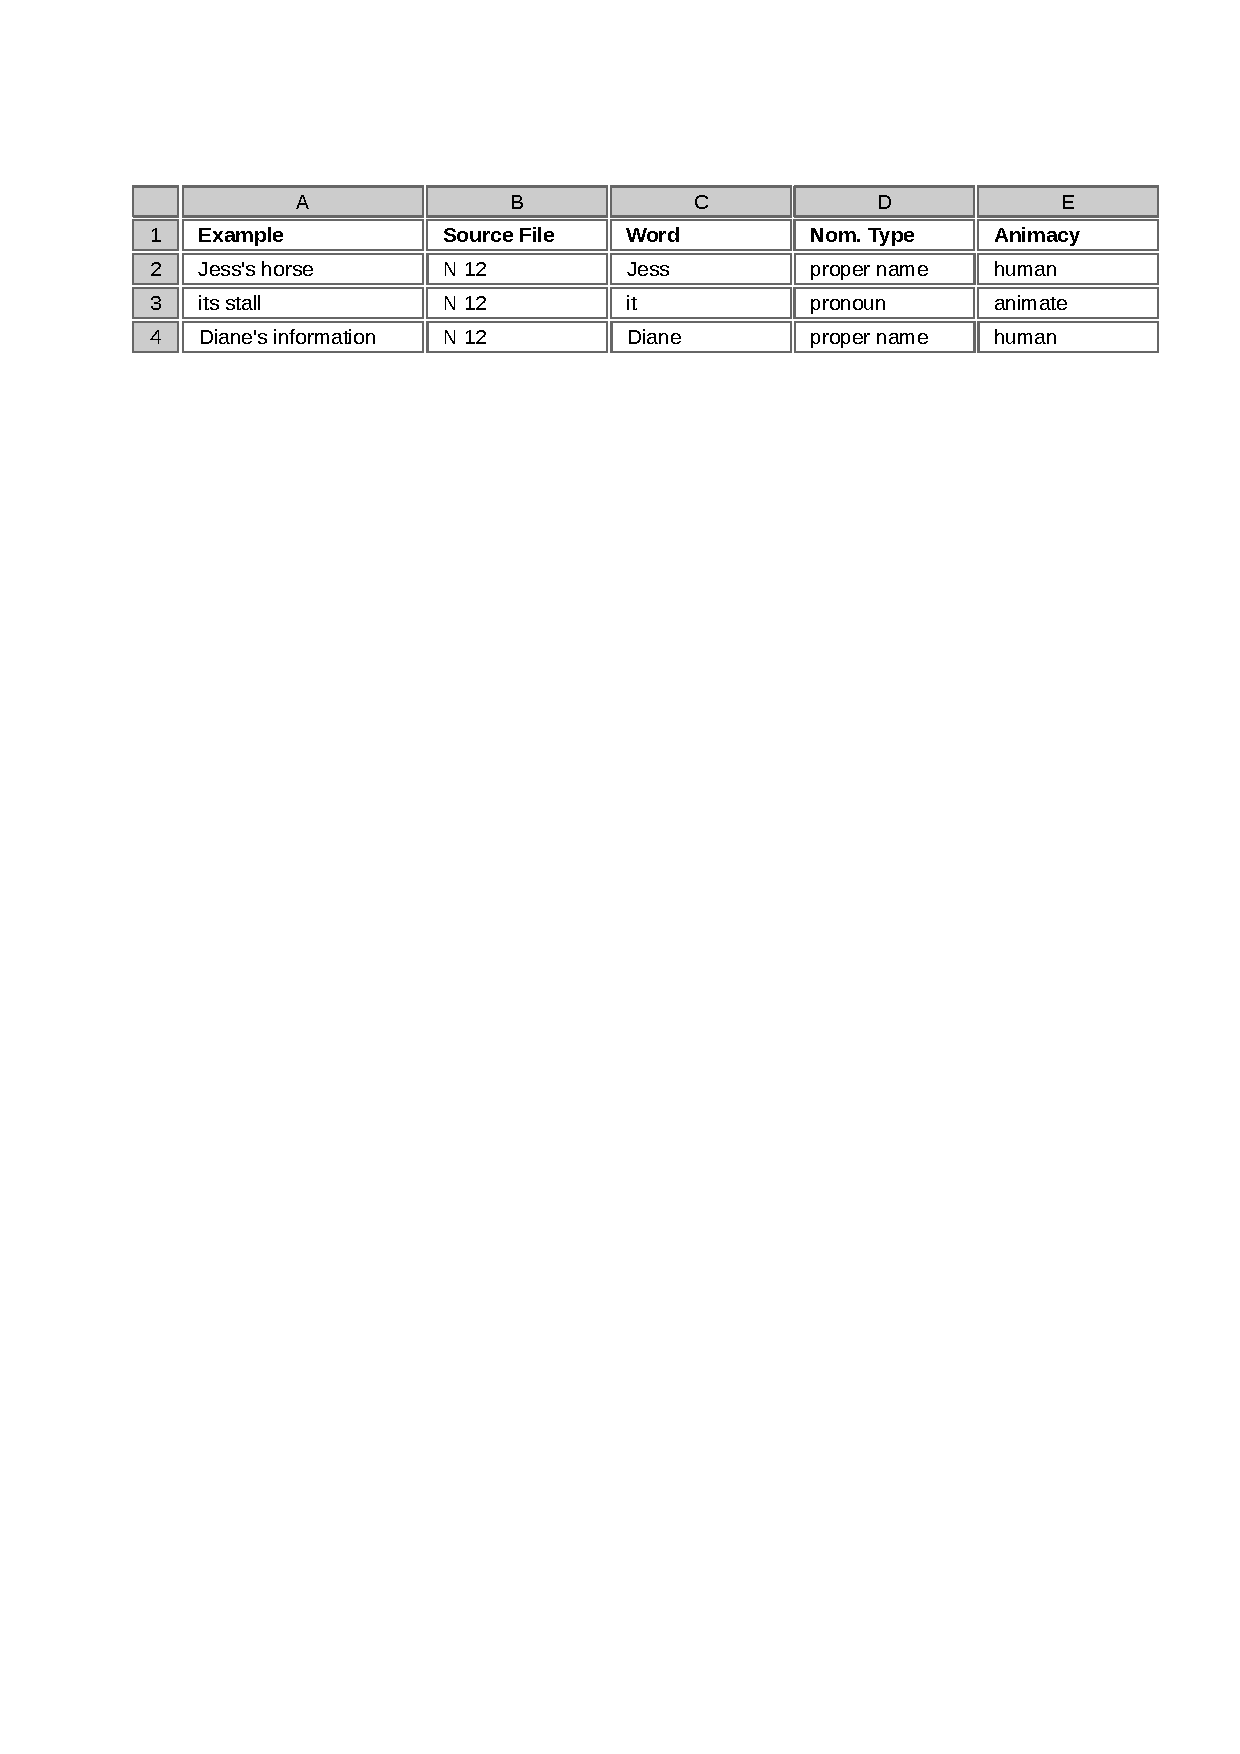
\includegraphics[width=\textwidth,keepaspectratio]{figures/storingdataright}
\end{figure}

The first line contains labels that tell us what information is found in each column respectively. This should include the example itself (either as shown in Figure \ref{fig:storingdataright}, or in the form of a KWIC concordance \is{KWIC concordance} line) and meta\hyp{}information such as what corpus and\slash or corpus file the example was extracted \is{retrieval} from. Crucially, it will include the relevant variables. Each subsequent line contains one observation \is{observational method} (i.e., one hit \is{hit} and the appropriate values of each variable). This format -- one column for each variable, and one line for each example -- is referred to as a \textit{raw data table}. It is the standard way of recording measurements \is{measurement} in all empirical sciences and we should adhere to it strictly, as it ensures that the \emph{structure} of the data is retained.

In particular, we should never store \is{data storage} our data in summarized form, for example, as shown in Figure \ref{fig:storingdatawrong}.

\begin{figure}[!htbp]
\caption{Data stored in summarized form}
\label{fig:storingdatawrong}
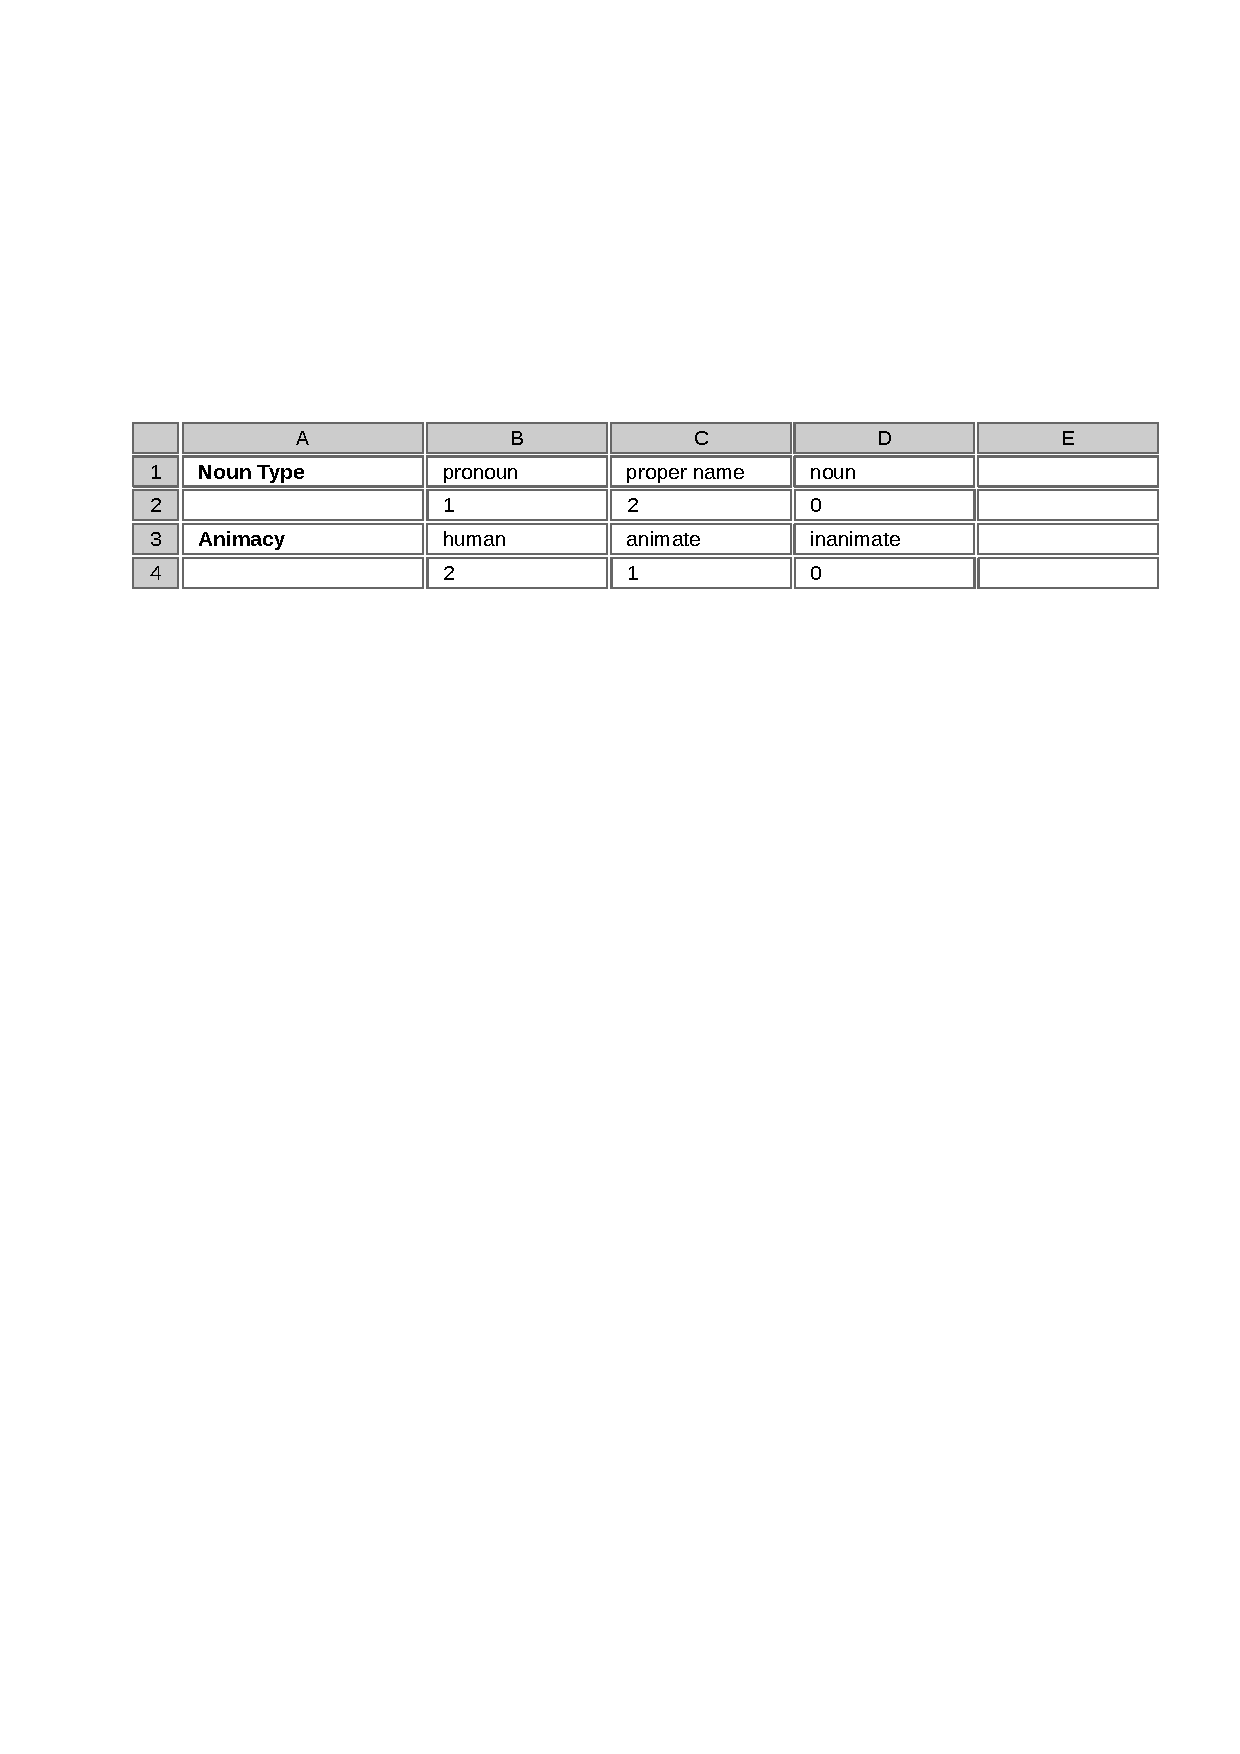
\includegraphics[width=\textwidth,keepaspectratio]{figures/storingdatawrong}
\end{figure}

There is simply no need to store \is{data storage} data in this form -- if we need this kind of summary, it can be created automatically from a raw data table like that in Figure \ref{fig:storingdataright} -- all major spreadsheet applications and statistical software packages have this functionality. What is more, statistics \is{statistics} software packages require a raw data table of the kind shown in Figure \ref{fig:storingdataright} as input for most kinds of statistical analysis.

As mentioned above, however, the format of storage \is{data storage} is not simply a practical matter, but a methodological one. If we did store our data in the form shown in Figure \ref{fig:storingdatawrong} straight away, we would irreversibly destroy the relationship between the corpus hits \is{hit} and the different annotations \is{annotation} applied to them. In other words, we would have no way of telling which combinations of variables actually occurred in the data. In Figure \ref{fig:storingdatawrong}, for example, we cannot tell whether the pronoun \is{pronoun} referred to one one of the human \is{animacy} referents or to the animate referent. Even if we do not need to know these relationships in the context of a given research project (or initially believe we will not), we should avoid this situation, as we do not know what additional questions may come up in the course of our research that do require this information.

Since quantitative \is{quantitative research} analysis always requires a raw data table, we might conclude that it is the only useful way of recording our annotation decisions. However, there are cases where it may be more useful to record them in the form of annotations \is{annotation} in (a copy of) the original corpus instead, i.e., analogously to automatically added annotations. For example, the information in Figure \ref{fig:storingdataright} could be recorded in the corpus itself in the same way that part\hyp{}of\hyp{}speech tags are, i.e., we could add an \textvv{Animacy} \is{animacy} label to every nominal \is{noun} element in our corpus in the format used for POS tags by the original version of the BROWN \is{BROWN} corpus, as shown in (\ref{ex:storingdatainline}):

\begin{exe}
\ex \begin{minipage}[t]{\textwidth} \raggedright \texttt{the\_AT} \texttt{fact\_NN\_\textbf{abstract}} \texttt{that\_CS} \texttt{Jess's\_NP\$\_\textbf{human}} \texttt{horse\_NN\_\textbf{animate}} \texttt{had\_HVD} \texttt{not\_*} \texttt{been\_BEN} \texttt{returned\_VBN} \texttt{to\_IN} \texttt{its\_PP\$\_\textbf{animate}} \texttt{stall\_NN\_\textbf{inanimate}} \texttt{could\_MD} \texttt{indicate\_VB} \texttt{that\_CS} \texttt{Diane's\_NP\$\_\textbf{human}} \texttt{information\_NN\_\textbf{abstract}} \texttt{had\_HVD} \texttt{been\_BEN} \texttt{wrong\_JJ} \texttt{,\_,} \texttt{but\_CC} \texttt{Curt\_NP\_\textbf{human}} \texttt{didn't\_DOD*} \texttt{interpret\_VB} \texttt{it\_PPO\_\textbf{inanimate}} \texttt{this\_DT} \texttt{way\_NN\_\textbf{inanimate}} \texttt{.\_.} \end{minipage}
\label{ex:storingdatainline}
\end{exe}

From a corpus annotated in \is{annotation} this way, we can always create a raw data list like that in Figure \ref{fig:storingdataright} by searching for possessives \is{possessive} and then separating the hits \is{hit} into the word itself, the \textvv{Part\hyp{}of\hyp{}Speech} label and the \textvv{Animacy} \is{animacy} annotation \is{annotation} (this can be done manually, or with the help of regular expressions in a text editor or with a few lines of code in a scripting language like Perl or Python).

The advantage would be that we, or other researchers, could also use our annotated \is{annotation} data for research projects concerned with completely different research questions. Thus, if we are dealing with a variable that is likely to be of general interest, we should consider the possibility of annotating the corpus itself, instead of first extracting \is{retrieval} the relevant data to a raw data table and annotating them afterwards. While the direct annotation of corpus files is rare in corpus linguistics, it has become the preferred strategy in various fields concerned with qualitative \is{qualitative research} analysis of textual data. There are open\hyp{}source and commercial software packages dedicated to this task. They typically allow the user to define a set of annotation \is{annotation} categories \is{categorization} with appropriate codes, \is{coding} import a text file, and then assign the codes to a word or larger textual unit by selecting it with the mouse and then clicking a button for the appropriate code that is then added (often in XML format) to the imported text. This strategy has the additional advantage that one can view one's annotated \is{annotation} examples in their original context (which may be necessary when annotating additional variables later). However, the available software packages are geared towards the analysis of individual texts and do not let the user to work comfortably with large \is{corpus size} corpora.

\chapter{Quantifying research questions}
\label{ch:quantifyingresearch}

Recall, once again, that at the end of Chapter \ref{ch:corpuslinguistics}, we defined corpus linguistics as

\begin{quotation}
the investigation of linguistic research questions that have been framed in terms of the conditional distribution \is{distribution, conditional} of linguistic phenomena in a linguistic corpus.
\end{quotation}

We discussed the fact that this definition covers cases of hypotheses \is{hypothesis} phrased in absolute terms, i.e. cases where the distribution of a phenomenon across different conditions is a matter of all or nothing (as in ``All speakers of American \is{American English} English refer to the front window of a car as \textit{windshield}; all speakers of British \is{British English} English refer to it as \textit{windscreen}'') as well as cases where the distribution is a matter of more\hyp{}or\hyp{}less (as in ``British \is{British English} English speakers prefer the word \textit{railway} over \textit{railroad} when referring to train tracks; American \is{American English} English speakers prefer \textit{railroad} over \textit{railway}'' or ``More British speakers refer to networks of train tracks as \textit{railway} instead of \textit{railroad}; more American English speakers refer to them as \textit{railroad} instead of \textit{railway}'').

In the case of hypotheses \is{hypothesis} stated in terms of more\hyp{}or\hyp{}less, predictions must be stated in quantitative \is{quantitative research} terms which in turn means that our data have to be quantified in some way so that we can compare them to our predictions. In this chapter, we will discuss in more detail how this is done when dealing with different types of data.

% me: Given that, as mentioned in Chapter \ref{ch:scientificmethod}, Section \ref{sec:scientifichypothesis}, hypotheses stated in relative terms are actually more typical in corpus linguistics than hypotheses stated in absolute terms, one might expect quantitative methods to be at the core of corpus-linguistic research practice. However, this is not the case. Many early corpus-linguistic studies chose to forgo quantification completely, or to treat it impressionistically (stating that one thing seemed to be more common in a given corpus or under a given condition than another). This has changed over the last twenty years, and even though the quantitatively apathetic and/or impressionistic schools of corpus linguistics are no longer dominant, they are still strong. In order to distinguish the more principled quantitative approach taken here from this impressionistic approach, it is now often referred to as \textit{Quantitative Corpus Linguistics} (a distinction first suggested in \citep{stefanowitsch_covarying_2005}, although the term is older).

Specifically, we will discuss three types of data (or ``levels of measurement'') \is{measurement} that we might encounter in the process of quantifying \is{quantitative research} the (annotated) \is{annotation} results of a corpus query \is{query} (Section \ref{sec:typesofdata}): nominal \is{nominal data} data (discussed in more detail in Section \ref{sec:descriptivenominal}), ordinal \is{ordinal data} (or rank) data (discussed in more detail in Section \ref{sec:descriptiveordinal}, and cardinal \is{cardinal data} data (discussed in more detail in Section \ref{sec:descriptivecardinal}. These discussions, summarized in Section \ref{sec:datatypessummary}, will lay the ground work for the introduction to statistical hypothesis \is{hypothesis} testing presented in the next chapter.

\section{Types of data}
\label{sec:typesofdata}

In order to illustrate these types of data, let us turn to a linguistic phenomenon that is more complex \is{complexity} than the distribution \is{distribution, conditional} of words across varieties, \is{language variety} and closer to the kind of phenomenon actually of interest to corpus linguists: that of the two English possessive \is{possessive} constructions introduced in Section \ref{sec:reliabilityannotationschemes} of Chapter \ref{ch:retrievalannotation} above. As discussed there, the two constructions can often be used seemingly interchangeably, as in (\ref{ex:sgenvsof}a, b):

\begin{exe}
\ex
\begin{xlist}
\label{ex:sgenvsof}
\ex \textit{The city's museums} are treasure houses of inspiring objects from all eras and cultures. (www.res.org.uk)
\ex Today one can find the monuments and artifacts from all of these eras in \textit{the museums of the city}. (www.travelhouseuk.co.uk)
\end{xlist}
\end{exe}

However, there are limits to this interchangeability. First, there are a number of relations that are exclusively encoded by the \textit{of}-construction, such as quantities (both generic, as in \textit{a couple\slash bit\slash lot of}, and in terms of measures, as in \textit{six miles\slash years\slash gallons of}), type relations (\textit{a kind\slash type\slash sort\slash class of}) and composition or constitution (\textit{a mixture of water and whisky}, \textit{a dress of silk}, etc.) \citep[cf., e.g.,][]{rohdenburg_constructional_2003}.

Second, and more interestingly, even where a relation \textit{can} be expressed by both constructions, there is often a preference for one or the other in a given context. A number of factors underlying these preferences have been suggested and investigated using quantitative \is{quantitative research} corpus\hyp{}linguistic methods. Among these, there are three that are widely agreed upon to have an influence, namely the givenness, \is{givenness} animacy \is{animacy} and weight \is{weight} of the modifier. These three factors nicely illustrate the levels of measurement \is{measurement} mentioned above, so we will look at each of them in some detail.

\textit{(a) Givenness}. \is{givenness} Following the principle of Functional Sentence Perspective, the \textit{s}-possessive \is{possessive} will be preferred if the modifier (the phrase marked by \textit{'s} or \textit{of}) refers to given information, while the construction with \textit{of} will be preferred if the modifier is new \citep{standwell_genitive_1982}. Thus, (\ref{ex:sgengivenness}a) and (\ref{ex:ofcgivennessb}a) sound more natural than (\ref{ex:sgengivenness}b) and (\ref{ex:ofcgivennessb}b) respectively:

\begin{exe}
\ex
\begin{xlist}
\label{ex:sgengivenness}
\ex In New York, we visited \textit{the city's} many museums.
\ex[\textsuperscript{??}]{In New York, we visited the many museums \textit{of the city}.}
\end{xlist}
\end{exe}

\begin{exe}
\ex
\begin{xlist}
\label{ex:ofcgivennessb}
\ex The Guggenheim is much larger than the museums \textit{of other major cities}.
\ex[\textsuperscript{??}]{The Guggenheim is much larger than \textit{other major cities'} museums.}
\end{xlist}
\end{exe}

\textit{(b) Animacy}. \is{animacy} Since animate referents tend to be more topical than inanimate ones and more topical elements tend to precede less topical ones, if the modifier is animate, \is{animacy} the \textit{s}-possessive \is{possessive} will be preferred, if it is inanimate, the construction with \textit{of} will be preferred (\citealt[cf.][192-203]{quirk_grammar_1972}; \citealt{deane_english_1987}):

\begin{exe}
\ex
\begin{xlist}
\label{ex:sgenanimacy}
\ex \textit{Solomon R. Guggenheim's} collection contains some fine paintings.
\ex[\textsuperscript{??}]{The collection \textit{of Solomon R. Guggenheim} contains some fine paintings.}
\end{xlist}
\end{exe}

\begin{exe}
\ex
\begin{xlist}
\label{ex:ofcanimacy}
\ex The collection \textit{of the Guggenheim museum} contains some fine paintings.
\ex[\textsuperscript{??}]{\textit{The Guggenheim museum's} collection contains some fine paintings.}
\end{xlist}
\end{exe}

\textit{(c) Length}. \is{length} Since short constituents generally precede long constituents, if the modifier is short, the \textit{s}-possessive \is{possessive} will be preferred, if it is long, the construction with \textit{of} will be preferred \citep{altenberg_binominal_1980}:

\begin{exe}
\ex
\begin{xlist}
\label{ex:sgenlength}
\ex \textit{The museum's} collection is stunning.
\ex[\textsuperscript{??}]{The collection \textit{of the museum} is stunning.
}\end{xlist}
\end{exe}

\begin{exe}
\ex
\begin{xlist}
\label{ex:ofclength}
\ex The collection \textit{of the most famous museum in New York} is stunning.
\ex[\textsuperscript{??}]{\textit{The most famous museum in New York's} collection is stunning.}
\end{xlist}
\end{exe}

In the case of all three factors, we are dealing with hypotheses \is{hypothesis} concerning preferences rather than absolute difference. None of the examples with question marks are ungrammatical \is{ungrammaticality} and all of them could conceivably occur; they just sound a little bit odd. Thus, the predictions we can derive from each hypothesis must be stated and tested in terms of relative rather than absolute differences -- they all involve predictions stated in terms more\hyp{}or\hyp{}less rather than all\hyp{}or\hyp{}nothing. Relative quantitative \is{quantitative research} differences are expressed and dealt with in different ways depending on the type of data they involve.

\subsection{Nominal data}
\label{sec:nominaldata}

A nominal \is{nominal data} variable is a variable whose values are labels for categories \is{categorization} that have no intrinsic order with respect to each other (i.e., there is no aspect of their definition that would allow us to put them in a natural order) -- for example, \textvv{Sex}, \textvv{Nationality} or \textvv{Native Language}. If we categorize \is{categorization} data in terms of such a nominal \is{nominal data} variable, the only way to quantify \is{quantitative research} them is to count the number of observations \is{observational method} of each category in a given sample and express the result in absolute frequencies \is{frequency} (i.e., raw numbers) or relative frequencies (such as percentages). For example, in the population of the world in 2005, there were 92 million native speakers of \textvv{german} and 75 million speakers of \textvv{french}.

We cannot \emph{rank} the values of nominal \is{nominal data} variables based on intrinsic criteria. For example, we cannot rank the German language higher than the French language on the basis of any intrinsic property of German and French. They are simply two different manifestations of the phenomenon \textvv{Language}, part of an unordered set including all human \is{animacy} languages.

That we cannot rank them based on intrinsic criteria does not mean that we cannot rank them at all. For example, we could rank them by number of speakers worldwide (in which case, as the numbers cited above show, German ranks above French). We could also rank them by the number of countries in which they are an official language (in which case French, which has official status in 29 countries, ranks above German, with an official status in only 6 countries). But the number of native speakers or the number of countries where a language has an official status is not an intrinsic property of that language -- German would still be German if its number of speakers was reduced by half by an asteroid strike, and French would still be French if it lost its official status in all 29 countries). In other words,
we are not really ranking \textvv{french} and \textvv{german} as values of \textvv{Language} at all; instead, we are ranking values of the variables \textvv{Size of Native Speech Community} and \textvv{Number of Countries with Official Language X} respectively.

We also cannot calculate mean \is{mean} values (``averages'') between the values of nominal \is{nominal data} variables. We cannot claim, for example, that Javanese is the mean of German and French because the number of Javanese native speakers falls (roughly) halfway between that of German and French native speakers. Again, what we would be calculating a mean of is the values of the variable \textvv{Size of Native Speech Community}, and while it makes a sort of sense to say that the mean \is{mean} of the values \textvv{number of french native speakers} and \textvv{number of german native speakers} was 83.5 in 2005, it does not make sense to refer to this mean as \textvv{number of javanese speakers}.

%me: We also cannot claim that English is the mean of German and French because its vocabulary is derived in equal proportions from the Germanic and the Romance language families...

With respect to the three hypotheses \is{hypothesis} concerning the distribution \is{distribution, conditional} of the \textit{s}-possessive \is{possessive} and the \textit{of}-possessive, it is obvious that they all involve at least one nominal \is{nominal data} variable -- the constructions themselves. These are essentially values of a variable we could call \textvv{Type of Possessive Construction}. We could categorize \is{categorization} all grammatical expressions of possession in a corpus in terms of the values \textvv{\textit{s}-possessive} and \textvv{\textit{of}-possessive}, count them and express the result in terms of absolute or relative frequencies. \is{frequency} For example, the \textit{s}-possessive occurs \num{22193} times in the BROWN \is{BROWN} corpus (excluding proper names and instances of the double \textit{s}-possessive), and the \textit{of}-possessive occurs \num{17800} times.\footnote{This is an estimate; it would take too long to go through all \num{36406} occurrences of \textit{of} and identify those that occur in the structure relevant here, so I categorized a random \is{chance} subsample of 500 hits of \textit{of} and generalized the proportion of \textit{of}-possessives \is{possessive} vs. other uses of \textit{of} to the total number of hits for \textit{of}.}

As with the example of the variable \textvv{Native Language} above, we can rank the constructions (i.e., the values of the variable \textvv{Type of Possessive \is{possessive} Construction}) in terms of their frequency \is{frequency} (the \textit{s}-possessive is more frequent), but again we are not ranking these values based on an intrinsic criterion but on an extrinsic one: their corpus frequency in one particular corpus. We can also calculate their mean \is{mean} frequency \is{frequency} (\num{19996.5}), but again, this is not a mean of the two constructions, but of their frequencies in one particular corpus.

\subsection{Ordinal data}
\label{sec:ordinaldata}

An ordinal \is{ordinal data} variable is a variable whose values are labels for categories \is{categorization} that \emph{do} have an intrinsic order with respect to each other but that cannot be expressed in terms of natural numbers. In other words, ordinal \is{ordinal data} variables are variables that are defined in such a way that some aspect of their definition allows us to order them without reference to an extrinsic criterion, but that does not give us any information about the distance (or degree of difference) between one category and the next. If we categorize \is{categorization} data in terms of such an ordinal \is{ordinal data} variable, we can treat them accordingly (i.e., we can rank them), or we can treat them like nominal \is{nominal data} data by simply ignoring their inherent order (i.e., we can still count the number of observations \is{observational method} for each value and report absolute or relative frequencies). \is{frequency} We cannot calculate mean \is{mean} values.

Some typical examples of ordinal \is{ordinal data} variables are demographic \is{demography} variables like \textvv{Education} or (in the appropriate sub\hyp{}demographic) \textvv{Military Rank}, but also \textvv{School Grades} and the kind of ratings often found in questionnaires (both of which are, however, often treated as though they were cardinal \is{cardinal data} data, see below).

For example, academic degrees are intrinsically ordered: it is part of the definition of a PhD degree that it ranks higher than a master's degree, which in turn ranks higher than a bachelor's degree. Thus, we can easily rank speakers in a sample of university graduates based on the highest degree they have completed. We can also simply count the number of PhDs, MAs, and BAs and ignore the ordering of the degrees. But we cannot calculate a mean: \is{mean} if five speakers in our sample of ten speakers have a PhD and five have a BA, this does not allow us to claim that all of them have an MA degree on average. The first important reason for this is that the size of the difference in terms of skills and knowledge that separates a BA from an MA is not the same as that separating an MA from a PhD: in Europe,
one typically studies two years for an MA, but it typically takes three to five years to complete a PhD. The second important reason is that the values of ordinal \is{ordinal data} variables typically differ along more than one dimension: while it is true that a PhD is a higher degree than an MA, which is a higher degree than a BA, the three degrees also differ in terms of specialization (from a relatively broad BA to a very narrow PhD), and the PhD degree differs from the two other degrees qualitatively: a BA and an MA primarily show that one has acquired knowledge and (more or less practical skills), but a PhD primarily shows that one has acquired research skills.

With respect to the three hypotheses \is{hypothesis} concerning the distribution \is{distribution, conditional} of the \textit{s}\hyp{}possessive \is{possessive} and the \textit{of}-possessive, clearly \textvv{Animacy} \is{animacy} is an ordinal \is{ordinal data} variable, at least if we think of it in terms of a scale, as we did in Chapter \ref{ch:scientificmethod}, Section \ref{sec:operationalization}. Recall that a simple animacy scale might look like this:

\begin{exe}
\ex \textvv{animate} > \textvv{inanimate} > \textvv{abstract}
\label{ex:simpleanimacyscale}
\end{exe}

On this scale, \textvv{animate} \is{animacy} ranks higher than \textvv{inanimate} which ranks higher than \textvv{abstract} \is{animacy} in terms of the property we are calling \textvv{Animacy}, and this ranking is determined by the scale itself, not by any extrinsic criteria.

This means that we could categorize \is{categorization} and rank all nouns in a corpus according to their animacy. But again, we cannot calculate a mean. \is{mean} If we have 50 \textvv{human} \is{animacy} nouns and 50 \textvv{abstract} nouns, we cannot say that we have 100 nouns with a mean value of \textvv{inanimate}. Again, this is because we have no way of knowing whether, in terms of animacy, \is{animacy} the difference between \textvv{animate} and \textvv{inanimate} is the same size as that between \textvv{inanimate} \is{animacy} and \textvv{abstract}, but also, because we are, again, dealing with qualitative as well as quantitative differences: the difference between animate and inanimate \is{animacy} on the one hand and abstract on the other is that the first two have physical existence; and the difference between animate on the one hand and inanimate \is{animacy} and abstract on the other is that animates are potentially alive and the other two are not. In other words, our scale is really a combination of at least two dimensions.

Again, we could ignore the intrinsic order of the values on our \textvv{Animacy} \is{animacy} scale and simply treat them as nominal \is{nominal data} data, i.e., count them and report the frequency \is{frequency} with which each value occurs in our data. Potentially ordinal \is{ordinal data} data are actually frequently treated like nominal data in corpus linguistics (cf. Section \ref{sec:mode}), and with complex ``scales'' combining a range of different dimensions, this is probably a good idea; but ordinal data also have a useful place in quantitative \is{quantitative research} corpus linguistics.

\subsection{Cardinal data}
\label{sec:cardinaldata}

Cardinal \is{cardinal data} variables are variables whose values are numerical measurements \is{measurement} along a particular dimension. In other words, they are intrinsically ordered (like ordinal \is{ordinal data} data), but not because some aspect of their definition allows us to order them, but because of their nature as numbers. Also, the distance between any two measurements is precisely known and can directly be expressed as a number itself. This means that we can perform any arithmetic operation on cardinal \is{cardinal data} data -- crucially, we can calculate means. Of course, we can also treat cardinal data like rank data \is{ordinal data} by ignoring all of their mathematical properties other than their order, and we can also treat them as nominal \is{nominal data} data.

Typical cases of cardinal \is{cardinal data} variables are demographic \is{demography} variables like \textvv{Age} or \textvv{Income}. For example, we can categorize \is{categorization} a sample of speakers by their age \is{age} and then calculate the mean \is{mean} age \is{age} of our sample. If our sample contains five 50\hyp{}year\hyp{}olds and five 30\hyp{}year\hyp{}olds, it makes perfect sense to say that the mean age \is{age} in our sample is 40; we might need additional information to distinguish between this sample and another sample that consists of 5 41\hyp{}year\hyp{}olds and 5 39\hyp{}year\hyp{}olds, that would also have a mean age \is{age} of 40 (cf. Chapter \ref{ch:significancetesting}), but the mean \is{mean} itself is meaningful, because the distance between 30 and 40 is the same as that between 40 and 50 and all measurements \is{measurement} involve just a single dimension (age). \is{age}

With respect to the two possessives, \is{possessive} the variables \textvv{Length} \is{length} and \textvv{Givenness} \is{givenness} are cardinal \is{cardinal data} variables. It should be obvious that we can calculate the mean \is{mean} length of words or other constituents in a corpus, a particular sample, a particular position in a grammatical construction, etc.

As mentioned above, we can also treat cardinal \is{cardinal data} data like ordinal \is{ordinal data} data. This may sometimes actually be necessary for mathematical reasons (see Chapter \ref{ch:significancetesting} below); in other cases, we may want to transform cardinal data to ordinal data based on theoretical considerations.

For example, the measure \is{measurement} of Referential Distance \is{referential distance} discussed in Chapter \ref{ch:scientificmethod}, Section \ref{sec:operationalization} yields cardinal \is{cardinal data} data ranging from 0 to whatever maximum distance we decide on and it would be possible, and reasonable, to calculate the mean \is{mean} referential distance of a particular type of referring expression. However \citet[20f]{givon_grammar_1992} argues that we should actually think of referential distance \is{referential distance} as ordinal \is{ordinal data} data: as most referring expressions consistently have a referential distance of either 0-1, or 2-3, or larger than 3, he suggests converting measures \is{measurement} of \textvv{Referential Distance} \is{referential distance} into just three categories: \is{categorization} \textvv{minimal gap} (0-1), \textvv{small gap} (2-3) and \textvv{long gap} (>3). Once we have done this, we can no longer calculate a mean, \is{mean} because the categories \is{categorization} are no longer equivalent in size or distance, \is{referential distance} but we can still rank them. Of course, we can also treat them as nominal \is{nominal data} data, simply counting the number of referring expressions in the categories \is{categorization} \textvv{minimal gap}, \textvv{small gap} and \textvv{long gap}.

\subsection{Interim summary}
\label{sec:datatypesinterim}

In the preceding three subsections, we have repeatedly mentioned concepts like \textit{frequency}, \is{frequency} \textit{percentage}, \textit{rank} and \textit{mean}. \is{mean} In the following three sections, we will introduce these concepts in more detail, providing a solid foundation of descriptive \is{description} statistical measures for nominal, \is{nominal data} ordinal \is{ordinal data} and cardinal \is{cardinal data} data.

Note, however, that most research designs, \is{research design} including those useful for investigating the hypotheses \is{hypothesis} about the two possessive \is{possessive} constructions, involve (at least) two variables: (at least) one independent variable and (at least) one dependent variable. Even our definition of corpus linguistics makes reference to this fact when it states that research questions should be framed such that it enables us to answer them by looking at the distribution \is{distribution, conditional} of linguistic phenomena across different conditions.

Since such conditions are most likely to be nominal \is{nominal data} in character (a set of language varieties, \is{language variety} groups of speakers, grammatical constructions, etc.), we will limit the discussion to combinations of variables where at least one variable is nominal, i.e., (a) designs \is{research design} with two nominal variables, (b) designs with one nominal and one ordinal \is{ordinal data} variable, and (c) designs with one nominal and one cardinal \is{cardinal data} variable. Logically, there are three additional designs, namely designs with (d) two ordinal variables, (e) two cardinal \is{cardinal data} variables or (f) one ordinal \is{ordinal data} and one cardinal \is{cardinal data} variable. For such cases, we would need different variants of correlation \is{correlation} analysis, which we will not discuss in this book in any detail (but there are pointers to the relevant literature in the Study Notes to Chapter \ref{ch:significancetesting} and we will touch upon such designs \is{research design} in some of the Case Studies in Part II of this book).

\section{Descriptive statistics for nominal data}
\label{sec:descriptivenominal}

Most examples we have looked at so far in this book involved two nominal \is{nominal data} variables: the independent variable \textvv{Variety} \is{language variety} (with the values \textvv{british \is{British English} english} vs. \textvv{american \is{American English} english}) and a dependent variable consisting of some linguistic alternation \is{alternation} (mostly regional synonyms \is{synonymy} of some lexicalized \is{lexicalization} concept). Thus, this kind of research design \is{research design} should already be somewhat familiar.

For a closer look, we will apply it to the first of the three hypotheses \is{hypothesis} introduced in the preceding section, which is restated here with the background assumption from which it is derived:

\begin{exe}
\ex Assumption: Discourse\hyp{}old items occur before discourse\hyp{}new items. \\
Hypothesis: \is{hypothesis} The \textvv{\textit{s}-possessive} \is{possessive} will be used when the modifier is \textvv{discourse\hyp{}old}, the \textvv{\textit{of}-possessive} will be used when the modifier is \textvv{discourse\hyp{}new}.
\label{ex:givennesshypothesis}
\end{exe}

Note that the terms \textvv{\textit{s}-possessive} \is{possessive} and \textvv{\textit{of}-possessive} are typeset in small caps in these hypotheses. \is{hypothesis} This is done in order to show that they are values of a variable in a particular research design, \is{research design} based on a particular theoretical construct. As such, these values must, of course, be given operational \is{operationalization} definitions (also, the construct upon which the variable is based should be explicated with reference to a particular model of language, but this would lead us too far from the purpose of this chapter and so I will assume that the phenomenon ``English nominal \is{noun} possession'' is self\hyp{}explanatory).

The definitions I used were the following:

\begin{exe}
\ex
\begin{xlist}
\label{ex:sgenofcdefinition}
\ex \textvv{\textit{s}-possessive}: \is{possessive} A construction consisting of a possessive pronoun \is{pronoun} or a noun \is{noun} phrase marked by the clitic \is{clitic} \textit{'s} modifying a noun following it, where the construction as a whole is not a proper name.
\ex \textvv{\textit{of}-possessive}: A construction consisting of a noun modified by a prepositional \is{adposition} phrase with \textit{of}, where the construction as a whole encodes a relation that could theoretically also be encoded by the \textvv{\textit{s}-possessive} and is not a proper name.
\end{xlist}
\end{exe}

Proper names (such as \textit{Scotty's Bar} or \textit{District of Columbia}) are excluded in both cases because they are fixed and could not vary. Therefore, they will not be subject to any restrictions concerning givenness, \is{givenness} animacy \is{animacy} or length. \is{length}

To turn these definitions into \emph{operational} \is{operationalization} definitions, we need to provide the specific queries \is{query} used to extract \is{retrieval} the data, including a description of those aspects of corpus annotation \is{annotation} used in formulating these queries. We also need annotation schemes detailing how to distinguish proper names from other uses and how to identify \textit{of}-constructions that encode relations that could also be encoded by the \textit{s}-possessive. \is{possessive}

The \textit{s}-possessive is easy to extract if we use the tagging \is{POS tagging} present in the BROWN \is{BROWN} corpus: words with the possessive clitic \is{clitic} (\textit{'s} or,for words whose stem \is{statistics} ends in \textit{s}, just \textit{'}) as well as possessive pronouns \is{pronoun} are annotated \is{annotation} with tags ending in the dollar sign \$, so a query \is{query} for words tagged in this way will retrieve \is{retrieval} all cases with high precision \is{precision} and recall. \is{recall} For the \textit{of}-possessive, \is{possessive} extraction \is{retrieval} is more difficult -- the safest way seems to be to search for words tagged \is{POS tagging} as nouns \is{noun} followed by the preposition \is{adposition} \textit{of}, which already excludes uses like [\textit{most of} NP] (where the quantifying expression is tagged as a post\hyp{}determiner) \is{determiner} [\textit{because of} NP], [\textit{afraid of} NP], etc.

The annotation \is{annotation} of the results for proper name or common noun status can be done in various ways -- in some corpora (but not in the BROWN \is{BROWN} corpus), the POS tags may help, in others, we might use capitalization as a hint, etc. The annotation for whether or not an \textit{of}-construction encodes a relation that could also be encoded by an \textit{s}-possessive \is{possessive} can be done as discussed in Section \ref{sec:reliabilityannotationschemes} of Chapter \ref{ch:retrievalannotation}.

Using these operationalizations \is{operationalization} for the purposes of the case studies in this chapter, I retrieved \is{retrieval} and annotated \is{annotation} a one\hyp{}percent sample of each construction (the constructions are so frequent that even one percent leaves us with 222 \textit{s}- and 178 \textit{of}-possessives \is{possessive} (the full data set for the studies presented in this and the following two subsections can be found in the Supplementary Online Material, file HKD3).

Next, the values \textvv{discourse\hyp{}old} and \textvv{discourse\hyp{}new} have to be operationalized. \is{operationalization} This could be done using the measure \is{measurement} of referential distance \is{referential distance} discussed in Section \ref{sec:operationalization} of Chapter \ref{ch:scientificmethod}, which (in slightly different versions) is the most frequently used operationalization in corpus linguistics. Since we want to demonstrate a design \is{research design} with two nominal \is{nominal data} variables, however, and in order to illustrate that constructs can be operationalized in different ways, I will use a different, somewhat indirect operationalization. It is well established that pronouns \is{pronoun} tend to refer to old information, whereas new information must be introduced using common nouns \is{noun} in full lexical NPs. Thus, we can assume a correlation \is{correlation} between the construct \textvv{discourse\hyp{}old} and the construct \textvv{pronoun} \is{pronoun} on the one hand, and the construct \textvv{discourse\hyp{}new} and the construct \textvv{common noun} on the other.

This correlation \is{correlation} is not perfect, as common nouns \is{noun} can also encode old information, so using \textvv{Part of Speech of Nominal Expression} as an operational \is{operationalization} definition for \textvv{Givenness} \is{givenness} is somewhat crude in terms of validity, \is{validity} but the advantage is that it yields a highly reliable, \is{reliability} easy\hyp{}to\hyp{}annotate \is{annotation} definition: we can use the part\hyp{}of\hyp{}speech tagging \is{POS tagging} to annotate our sample automatically.

We can now state the following quantitative \is{quantitative research} prediction based on our hypothesis: \is{hypothesis}

\begin{exe}
\ex Prediction: There will be more cases of the \textvv{\textit{s}-possessive} \is{possessive} with \textvv{discourse\hyp{}old} modifiers than with \textvv{discourse\hyp{}new} modifiers, and more cases of the \textvv{\textit{of}-possessive} with discourse\hyp{}new modifiers than with \textvv{discourse\hyp{}old} modifiers.
\label{ex:givennessprediction}
\end{exe}

Table \ref{tab:posmodpossesives} shows the absolute frequencies \is{frequency} of the parts of speech of the modifier in both constructions (examples with proper names were discarded, as the givenness \is{givenness} of proper names in discourse is less predictable than that of pronouns \is{pronoun} and common nouns): \is{noun}

\begin{table}[!htbp]
\caption{Part of speech of the modifier in the \textit{s}-possessive and the \textit{of}-possessive}
\label{tab:posmodpossesives}
\begin{tabular}[t]{llccr}
\lsptoprule
 & & \multicolumn{2}{c}{\textvv{Possessive}} & \\
 & & \textvv{\textit{s}-possessive} & \textvv{\textit{of}-possessive} & Total \\
\midrule
\textvv{Givenness} & \textvv{old} & 180 & 3 & 183 \\
 & \textvv{new} & 20 & 153 & 173 \\
\midrule
 & Total & 200 & 156 & 356 \\
\lspbottomrule
\end{tabular}
\end{table}

Such a table, examples of which we have already seen in previous chapters, is referred to as a \textit{contingency table}. \is{contingency table} In this case, the contingency table consists of four cells showing the frequencies \is{frequency} of the four intersections of the variables \textvv{Givenness}, \is{givenness} (with the values \textvv{new}, i.e. ``pronoun'', \is{pronoun} and \textvv{old}, i.e. ``common noun'' \is{noun} and \textvv{Possessive} \is{possessive} (with the values \textvv{s} and \textvv{of}); in other words, it is a two\hyp{}by\hyp{}two table. Possessive is presented as the dependent variable here, since logically the hypothesis \is{hypothesis} is that the information status of the modifier influences the choice of construction, but mathematically it does not matter in contingency \is{contingency table} tables what we treat as the dependent or independent variable.

In addition, there are two cells showing the \textit{row totals} (the sum of all cells in a given row) and the \textit{column totals} (the sum of all cells in a given column), and one cell showing the \textit{table total} (the sum of all four intersections). The row and column totals for a given cell are referred to as the \textit{marginal frequencies} \is{frequency} for that cell.

\subsection{Percentages}
\label{sec:percentages}

The frequencies \is{frequency} in Table \ref{tab:posmodpossesives} are fairly easy to interpret in this case, because the differences in frequency are very clear. However, we should be wary of basing our assesment of corpus data directly on raw frequencies in a contingency \is{contingency table} table. These can be very misleading, especially if the marginal frequencies \is{frequency} of the variables differ substantially, which in this case, they do: the \textit{s}-possessive \is{possessive} is more frequent overall than the \textit{of}-possessive and discourse\hyp{}old modifiers (i.e., pronouns) \is{pronoun} are slightly more frequent overall than discourse\hyp{}new ones (i.e., common nouns). \is{noun}

Thus, it is generally useful to convert the absolute frequencies \is{frequency} to relative frequencies, abstracting away from the differences in marginal frequencies. In order to convert an absolute frequency \textit{n} into a relative one, we simply divide it by the total number of cases \textit{N} of which it is a part. This gives us a decimal fraction expressing the frequency \is{frequency} as a proportion of 1. If we want a percentage instead, we multiply this decimal fraction by 100, thus expressing our frequency as a proportion of 100.

For example, if we have a group of 31 students studying some foreign language and six of them study German, the percentage of students studying German is

$$\frac{6}{31} = 0.1935.$$

Multiplying this by 100, we get

$$0.1953 \times 100 = 19.35\%$$

In other words, a percentage is just another way of expressing a decimal fraction, which is just another way of expressing a fraction, all of which are (among other things) ways of expressing relative frequencies \is{frequency} (i.e., proportions). In academic papers, it is common to report relative frequencies as decimal fractions rather than as percentages, so we will follow this practice here.

If we want to convert the absolute frequencies \is{frequency} in Table \ref{tab:posmodpossesives} into relative frequencies, we first have to decide what the relevant total \emph{N} is. There are three possibilities, all of which are useful in some way: we can divide each cell by its column total, by its row total or by the table total. Table \ref{tab:absrelfreqposs} shows the results for all three possibilities.

The column proportions can be related to our prediction most straightforwardly: based on our hypothesis, \is{hypothesis} we predicted that in our sample a majority of \textit{s}-possessives \is{possessive} should have modifiers that refer to discourse\hyp{}old information and, conversely a majority of \textit{of}-possessives \is{possessive} should have modifiers that refer to discourse\hyp{}new information.

The relevance of the row proportions is less clear in this case. We might predict, based on our hypothesis, \is{hypothesis} that the majority of modifiers referring to old information should occur in \textit{s}-possessives \is{possessive} and the majority of modifiers referring to new information should occur in \textit{of}-possessives.

\begin{table}[!htbp]
\caption{Absolute and relative frequencies of the modifier's givenness (as reflected in its part of speech) in the English possessive constructions}
\label{tab:absrelfreqposs}
\begin{tabular}[t]{lllccr}
\lsptoprule
 & & & \multicolumn{2}{c}{\textvv{Possessive}} & \\
 & & & \textvv{\textit{s}-possessive} & \textvv{\textit{of}-possessive} & Total \\
\midrule
\textvv{\makecell[lt]{Discourse \\Status}} & \textvv{old} & \makecell[lt]{\footnotesize{\textit{Abs.}}\\\footnotesize{\textit{Rel. (Col.)}}\\\footnotesize{\textit{Rel. (Row)}}\\\footnotesize{\textit{Rel. (Tab.)}}} & \makecell[t]{180\\0.9000\\0.9836\\0.5056} & \makecell[t]{3\\0.0192\\0.0164\\0.0084} & \makecell[t]{183\\--\\1.0000\\0.5140} \\
 & \textvv{new} & \makecell[lt]{\footnotesize{\textit{Abs.}}\\\footnotesize{\textit{Rel. (Col.)}}\\\footnotesize{\textit{Rel. (Row)}}\\\footnotesize{\textit{Rel. (Tab.)}}} & \makecell[t]{20\\0.1000\\0.1156\\0.0562} & \makecell[t]{153\\0.9808\\0.8844\\0.4298} & \makecell[t]{173\\--\\1.0000\\0.4860} \\
\midrule
 & Total & \makecell[lt]{\footnotesize{\textit{Abs.}}\\\footnotesize{\textit{Rel. (Col.)}}\\\footnotesize{\textit{Rel. (Row)}}\\\footnotesize{\textit{Rel. (Tab.)}}} & \makecell[t]{200\\1.0000\\--\\0.5618} & \makecell[t]{156\\1.0000\\--\\0.4382} & \makecell[t]{356\\1.0000\\1.0000\\1.0000} \\
\lspbottomrule
\end{tabular}
\end{table}
% layout: Please do NOT align the numbers in this table at the decimal point, as it would look very ugly and also does not make sense.

This is the case in Table \ref{tab:absrelfreqposs}, and this is certainly compatible with our hypothesis. \is{hypothesis} However, if it were not the case, this could also be compatible with our hypothesis. Note that the constructions differ in frequency, \is{frequency} with the \textit{of}-possessive \is{possessive} being only three\hyp{}quarters as frequent as the \textit{s}-possessive. Now imagine the difference was ten to one instead of four to three. In this case, we might well find that the majority of both old and new modifiers occurs in the \textit{s}-possessives, simply because there are so many more \textit{s}-possessives than \textit{of}-possessives. We would, however, expect the majority to be larger in the case of old modifiers than in the case of new modifiers. In other words, even if we are looking at row percentages, the relevant comparisons are across rows, not within rows.

Whether column or row proportions are more relevant to a hypothesis \is{hypothesis} depends, of course, on the way variables are arranged in the table: if we rotate the table such that the variable \textvv{Possessive} \is{possessive} ends up in the rows, then the row proportions would be more relevant. When interpreting proportions in a contingency \is{contingency table} table, we have to find those that actually relate to our hypothesis. In any case, the interpretation of both row and column proportions requires us to choose one value of one of our variables and compare it across the two values of the other variable, and then compare this comparison to a comparison of the other value of that variable. If that sounds complicated, this is because it \textit{is} complicated.

It would be less confusing if we had a way of taking into account both values of both variables at the same time. The table proportions allow this to some extent. The way our hypothesis \is{hypothesis} is phrased, we would expect a majority of cases to instantiate the intersections \textvv{\textit{s}-possessive} \is{possessive} $\cap$ \textvv{discourse\hyp{}old} and \textvv{\textit{of}\hyp{}possessive} $\cap$ \textvv{discourse\hyp{}new}, with a minority of cases instantiating the other two intersections. In Table \ref{tab:absrelfreqposs}, this is clearly the case: the intersection \textvv{\textit{s}-possessive} $\cap$ \textvv{discourse\hyp{}old} contains more than fifty percent of all cases, the intersection \textvv{\textit{of}-possessive} $\cap$ \textvv{discourse\hyp{}new} well over 40 percent. Again, if the marginal frequencies \is{frequency} differ more extremely, so may the table percentages in the relevant intersections. We could imagine a situation, for example, where 90 percent of the cases fell into the intersection \textvv{\textit{s}-possessive} \is{possessive} $\cap$ \textvv{discourse\hyp{}old} and 10 percent in the intersection \textvv{\textit{of}-possessive} $\cap$ \textvv{discourse\hyp{}new} -- this would still be a corroboratation \is{corroboration} of our hypothesis. \is{hypothesis}

While relative frequencies \is{frequency} (whether expressed as decimal fractions or as percentages) are, with due care, more easily interpretable than absolute frequencies, they have two disadvantages. First, by abstracting away from the absolute frequencies, \is{frequency} we lose valuable information: we would interpret a distribution \is{distribution, conditional} such as that in Table \ref{tab:formulaexpected} differently, if we knew that it was based on a sample on just 35 instead of 356 corpus hits. Second, it provides no sense of how different our observed distribution is from the distribution that we would expect if there was no relation between our two variables, i.e., if the values were distributed randomly. \is{chance} Thus, instead of (or in addition to) using relative frequencies, \is{frequency} we should compare the \emph{observed} absolute frequencies of the intersections of our variables with the \emph{expected} \is{frequency, expected} absolute frequencies, i.e., the absolute frequencies \is{frequency} we would expect if there was a random relationship between the variables. This comparison between observed and expected frequencies also provides a foundation for inferential statistics, \is{statistics} discussed in Chapter \ref{ch:significancetesting}.

\subsection{Observed and expected frequencies}
\label{sec:observedexpected}

So how do we determine the expected \is{frequency, expected} frequencies \is{frequency} of the intersections of our variables? Consider the textbook example of a random \is{chance} process: flipping a coin onto a hard surface. Ignoring the theoretical and extremely remote possibility that the coin will land, and remain standing, on its edge, there are two possible outcomes, ``heads'' and ``tails''. If the coin has not been manipulated in some clever way, for example, by making one side heavier than the other, the probability \is{probability} for heads and tails is 0.5 (or fifty percent) each (such a coin is called a ``fair coin'' in statistics). \is{statistics}

From these probabilities, \is{probability} we can calculate the expected \is{frequency, expected} \is{frequency} frequency of heads and tails in a series of coin flips. If we flip the coin ten times, we expect five heads and five tails, because $0.5 \times 10 = 5$. If we flip the coin 42 times, the expected frequency \is{frequency} is 21 for heads and 21 for tails ($0.5 \times 42$), and so on. In the real world, we would of course expect some variation \is{variation} (more on this in Chapter \ref{ch:significancetesting}), so ``expected frequency'' refers to a theoretical expectation derived by multiplying the probability \is{probability} of an event by the total number of observations. \is{observational method}

So how do we transfer this logic to a contingency \is{contingency table} table like Table \ref{tab:posmodpossesives}? Naively, we might assume that the expected \is{frequency, expected} \is{frequency} frequencies for each cell can be determined by taking the total number of observations and dividing it by four: if the data were distributed \is{distribution, conditional} randomly, \is{chance} each intersection of values should have about the same frequency (just like, when tossing a coin, each side should come up roughly the same number of times). However, this would only be the case if all marginal frequencies \is{frequency} were the same, for example, if our sample contained fifty \textvv{\textit{s}-possessives} \is{possessive} and fifty \textvv{\textit{of}-possessives} and fifty of the modifiers were discourse old (i.e. pronouns) \is{pronoun} and fifty of them were discourse\hyp{}new (i.e. common nouns). \is{noun} But this is not the case: there are more discourse\hyp{}old modifiers than discourse\hyp{}new ones (183 vs. 173) and there are more \textit{s}-possessives than \textit{of}-possessives (200 vs. 156).

These marginal frequencies of our variables and their values are a fact about our data that must be taken as a given when calculating the expected \is{frequency, expected} frequencies: our hypothesis \is{hypothesis} says nothing about the overall frequency of the two constructions or the overall frequency \is{frequency} of discourse\hyp{}old and discourse\hyp{}new modifiers, but only about the frequencies with which these values should co\hyp{}occur. In other words, the question we must answer is the following: Given that the \textit{s}- and the \textit{of}-possessive \is{possessive} occur 200 and 156 times respectively and given that there are 183 discourse\hyp{}old modifiers and 173 discourse\hyp{}new modifiers, how frequently would each combination these values occur by chance? \is{chance}

Put like this, the answer is conceptually quite simple: the marginal frequencies should be distributed \is{distribution, conditional} across the intersections of our variables such that the relative frequencies \is{frequency} in each row should be the same as those of the row total and the relative frequencies in each column should be the same as those of the column total.

For example, 56.18 percent of all possessive \is{possessive} constructions in our sample are \textit{s}-possessives and 43.82 percent are \textit{of}-possessives; if there were a random relationship between type of construction and givenness \is{givenness} of the modifier, we should find the same proportions for the 183 constructions with old modifiers, i.e. $183 \times 0.5618 = 102.81$ \textit{s}-possessives and $183 \times 0.4382 = 80.19$ \textit{of}-possessives. Likewise, there are 173 constructions with new modifiers, so $173 \times 0.5618 = 97.19$ of them should be \textit{s}-possessives and $173 \times 0.4382 = 75.81$ of them should be \textit{of}-possessives. The same goes for the columns: 51.4 percent of all constructions have old modifiers and 41.6 percent have new modifiers. If there were a random \is{chance} relationship between type of construction and givenness \is{givenness} of the modifier, we should find the same proportions for both types of possessive \is{possessive} construction: there should be $200 \times 0.514 = 102.8$ \textit{s}-possessives with old modifiers and 97.2 with new modifiers, as well as $156 \times 0.514 = 80.18$ \textit{of}-possessives with old modifiers and $156 \times 0.486 = 75.82$ \textit{of}-possessives with new modifiers. Note that the expected \is{frequency, expected} \is{frequency} frequencies for each intersection are the same whether we use the total row percentages or the total column percentages: the small differences are due to rounding errors.

To avoid rounding errors, we should not actually convert the row and column totals to percentages at all, but use the following much simpler way of calculating the expected \is{frequency, expected} frequencies: for each cell, we simply multiply its marginal frequencies and divide the result by the table total as shown in Table \ref{tab:formulaexpected}; note that we are using the standard convention of using \textit{O} to refer to observed frequencies, \is{frequency, observed} \textit{E} to refer to expected frequencies, and subscripts to refer to rows and columns. The convention for these subscripts is as follows: use \textit{1} for the first row or column, \textit{2} for the second row or column, and \textit{T} for the row or column total, and give the index for the row before that of the column. For example, \textit{E}\textit{\textsubscript{21}} refers to the expected \is{frequency, expected} frequency of the cell in the second row and the first column, \textit{O}\textit{\textsubscript{1T}} refers to the total of the first row, and so on.

\begin{table}[!htbp]
\caption{Calculating expected frequencies from observed frequencies}
\label{tab:formulaexpected}
\begin{tabular}[t]{llccr}
\lsptoprule
 & & \multicolumn{2}{c}{\textvv{Dependent Variable}} & \\
 & & \textvv{value 1} & \textvv{value 2} & Total \\
\midrule
\textvv{\textvv{\makecell[lt]{Independent \\Variable}}} & \textvv{value 1} & \makecell[lt]{$\displaystyle{E_{\mathit{11}} = \frac{O_{\mathit{T1}} \times O_{\mathit{1T}}}{O_{\mathit{TT}}}}$} & $\displaystyle{E_{\mathit{12}} = \frac{O_{\mathit{T2}} \times O_{\mathit{1T}}}{O_{\mathit{TT}}}}$ & $O_{\mathit{1T}}$ \\
 & \textvv{value 2} & $\displaystyle{E_{\mathit{21}} = \frac{O_{\mathit{T1}} \times O_{\mathit{2T}}}{O_{\mathit{TT}}}}$ & $\displaystyle{E_{\mathit{22}} = \frac{O_{\mathit{T2}} \times O_{\mathit{2T}}}{O_{\mathit{TT}}}}$ & $O_{\mathit{2T}}$ \\
\midrule
 & Total & $O_{\mathit{T1}}$ & $O_{\mathit{T2}}$ & $O_{\mathit{TT}}$ \\
\lspbottomrule
\end{tabular}
\end{table}

Applying this procedure to our observed frequencies \is{frequency, observed} yields the results shown in Table \ref{tab:obsexpfreqposs}. One should always report nominal \is{nominal data} data in this way, i.e., giving both the observed and the expected \is{frequency, expected} frequencies in the form of a contingency \is{contingency table} table.

\begin{table}[!htbp]
\caption{Observed and expected frequencies of old and new modifiers in the \textit{s}- and the \textit{of}-possessive}
\label{tab:obsexpfreqposs}
\begin{tabular}[t]{lllccr}
\lsptoprule
 & & & \multicolumn{2}{c}{\textvv{Possessive}} & \\
 & & & \textvv{\textit{s}-possessive} & \textvv{\textit{of}-possessive} & Total \\
\midrule
\textvv{\makecell[lt]{Discourse \\Status}} & \textvv{old} & \makecell[lt]{\footnotesize{\textit{Obs.}}\\\footnotesize{\textit{Exp.}}} & \makecell[t]{180\\102.81} & \makecell[t]{3\\80.19} & \makecell[t]{183\\} \\
 & \textvv{new} & \makecell[lt]{\footnotesize{\textit{Obs.}}\\\footnotesize{\textit{Exp.}}} & \makecell[t]{20\\97.19} & \makecell[t]{153\\75.81} & \makecell[t]{173\\} \\
\midrule
 & Total & \makecell[lt]{\textit{Obs.}} & \makecell[t]{200} & \makecell[t]{156} & \makecell[t]{356} \\
\lspbottomrule
\end{tabular}
\end{table}

We can now compare the observed and expected \is{frequency, expected} frequencies of each intersection to see whether the difference conforms to our quantitative \is{quantitative research} prediction. This is clearly the case: for the intersections \textvv{\textit{s}-possessive} \is{possessive} $\cap$ \textvv{discourse\hyp{}old} and \textvv{\textit{of}-possessive} $\cap$ \textvv{discourse\hyp{}new}, the observed frequencies \is{frequency, observed} are higher than the expected ones, for the intersections \textvv{\textit{s}-possessive} $\cap$ \textvv{discourse\hyp{}new} and \textvv{\textit{of}-possessive} $\cap$ \textvv{discourse\hyp{}old}, the observed frequencies are lower than the expected ones.

This conditional distribution \is{distribution, conditional} seems to corroborate \is{corroboration} our hypothesis. \is{hypothesis} However, note that it does not yet prove or disprove anything, since, as mentioned above, we would never expect a real\hyp{}world distribution of events to match the expected distribution perfectly. We will return to this issue in \ref{ch:significancetesting}.

% me: Footnote showing how obs/exp can be used to calculate $\kappa$

\section{Descriptive statistics for ordinal data}
\label{sec:descriptiveordinal}

Let us turn, next, to a design \is{research design} with one nominal \is{nominal data} and one ordinal \is{ordinal data} variable: a test of the second of the three hypotheses \is{hypothesis} introduced at the beginning of this chapter. Again, it is restated here together with the background assumption from which it is derived:

\begin{exe}
\ex Assumption: Animate \is{animacy} items occur before inanimate items. \\
Hypothesis: \is{hypothesis} The \textvv{\textit{s}-possessive} will be used when the modifier is high in \textvv{Animacy}, the \textvv{\textit{of}-possessive} \is{possessive} will be used when the modifier is low in \textvv{Animacy}.
\label{ex:animacyhypothesis}
\end{exe}

The constructions are operationalized \is{operationalization} as before. The data used are based on the same data set, except that cases with proper names are now included. For expository reasons, we are going to look at a ten\hyp{}percent subsample of the full sample, giving us 22 \textit{s}-possessives \is{possessive} and 17 \textit{of}-possessives.

\textvv{Animacy} \is{animacy} was operationally defined in terms of the annotation \is{annotation} scheme shown in Table \ref{tab:animacyannotationscheme} (based on \citealt{zaenen_animacy_2004}).

\begin{table}[!htbp]
\caption{A simple annotation scheme for \textvv{Animacy}}
\label{tab:animacyannotationscheme}
\resizebox{\textwidth}{!}{
\begin{tabular}[t]{lllr}
\lsptoprule
\textvv{Animacy Category} & & Definition & Rank \\
\midrule
\textvv{human} & (\textvv{hum}) & Real or fictional humans and human\hyp{}like beings & 1 \\
\textvv{organization} & (\textvv{org}) & Groups of humans acting with a common purpose & 2 \\
\textvv{other animate} & (\textvv{ani}) & Real or fictional animals, animal\hyp{}like beings and plants & 3 \\
\textvv{human attribute} & (\textvv{hat}) & Body parts, organs, etc. of humans & 4 \\
\textvv{concrete touchable} & (\textvv{cct}) & Physical entities that are incapable of life and can be touched & 5 \\
\textvv{concrete nontouchable} & (\textvv{ccn}) & Physical entities that are incapable of life and cannot be touched & 6 \\
\textvv{location} & (\textvv{loc}) & Physical places and regions & 7 \\
\textvv{time} & (\textvv{tim}) & Points in and periods of time & 8 \\
\textvv{event} & (\textvv{evt}) & Events & 9 \\
\textvv{abstract} & (\textvv{abs}) & Other abstract entities & 10 \\
\lspbottomrule
\end{tabular}}
\end{table}

As pointed out above, \textvv{Animacy} hierarchies are a classic example of ordinal \is{ordinal data} data, as the categories \is{categorization} can be ordered (although there may be some disagreement about the exact order), but we cannot say anything about the distance between one category and the next, and there is more than one conceptual dimension involved (I ordered them according to dimensions like ``potential for life'', ``touchability'' and ``conceptual independence'').

We can now formulate the following prediction:

\begin{exe}
\ex Prediction: The modifiers of the \textvv{\textit{s}-possessive} \is{possessive} will tend to occur high on the \textvv{Animacy} scale, the modifiers of the \textvv{\textit{of}-possessive} will tend to occur low on the \textvv{Animacy} scale.
\label{ex:animacyprediction}
\end{exe}

Note that phrased like this, it is not yet a quantitative \is{quantitative research} prediction, since ``tend to'' is not a mathematical concept. While \textit{frequency} \is{frequency} for nominal \is{nominal data} data and \textit{mean} \is{mean} (or ``average'') for cardinal \is{cardinal data} data are used in everyday language with something close to their mathematical meaning, we do not have an everyday word for dealing with differences in ordinal \is{ordinal data} data. We will return to this point presently, but first, let us look at the data impressionistically. Table \ref{tab:sampleanimacysgenofc} shows the annotated \is{annotation} sample (cases are listed in the order in which they occurred in the corpus).

\begin{table}[!htbp]
\caption{A sample of \textit{s}- and \textit{of}-possessives annotated for \textvv{Animacy} (BROWN)}
\label{tab:sampleanimacysgenofc}
\resizebox*{!}{\textheight}{
\begin{tabular}[t]{rllr}
\lsptoprule
No. & Example & \textvv{Animacy} & Rank \\
\midrule
(a) & \multicolumn{3}{l}{\textvv{\textit{s}-possessive}} \\
\midrule
1 & \textit{its [administration] policy} & \textvv{org} & 2 \\
2 & \textit{her professional roles} & \textvv{hum} & 1 \\
3 & \textit{their burden} & \textvv{hum} & 1 \\
4 & \textit{its [word] musical frame} & \textvv{ccn} & 6 \\
5 & \textit{its [sect] metaphysic} & \textvv{org} & 2 \\
6 & \textit{your management climate} & \textvv{org} & 2 \\
7 & \textit{their families} & \textvv{hum} & 1 \\
8 & \textit{Lumumba's death} & \textvv{hum} & 1 \\
9 & \textit{his arts or culture} & \textvv{hum} & 1 \\
10 & \textit{her life} & \textvv{hum} & 1 \\
11 & \textit{its [monument] reputation} & \textvv{cct} & 5 \\
12 & \textit{their impulses and desires} & \textvv{hum} & 1 \\
13 & \textit{its [board] members' duties} & \textvv{org} & 2 \\
14 & \textit{our national economy} & \textvv{org} & 2 \\
15 & \textit{the convict's climactic reappearance} & \textvv{hum} & 1 \\
16 & \textit{its [bird] wing} & \textvv{ani} & 3 \\
17 & \textit{her father} & \textvv{hum} & 1 \\
18 & \textit{his voice} & \textvv{hum} & 1 \\
19 & \textit{her brain} & \textvv{hum} & 1 \\
20 & \textit{his brown face} & \textvv{hum} & 1 \\
21 & \textit{his expansiveness} & \textvv{hum} & 1 \\
22 & \textit{its [snake] black, forked tongue} & \textvv{ani} & 3 \\
23 & \textit{the novelist's carping phrase} & \textvv{hum} & 1 \\
\midrule
(b) & \multicolumn{3}{l}{\textvv{\textit{of}-possessive}} \\
\midrule
1 & \textit{the invasion of Cuba} & \textvv{loc} & 8 \\
2 & \textit{a joint session of Congress} & \textvv{org} & 2 \\
3 & \textit{[...] enemies of peaceful coexistence} & \textvv{evt} & 7 \\
4 & \textit{the word of God} & \textvv{hum} & 1 \\
5 & \textit{the volume of the cylinder opening [...]} & \textvv{cct} & 5 \\
6 & \textit{the depths of the fourth dimension} & \textvv{abs} & 10 \\
7 & \textit{the views of George Washington} & \textvv{hum} & 1 \\
8 & \textit{all the details of the pattern} & \textvv{abs} & 10 \\
9 & \textit{the makers of constitutions} & \textvv{ccn} & 6 \\
10 & \textit{the extent of ethical robotism} & \textvv{abs} & 10 \\
11 & \textit{the number of new [...] construction projects [...]} & \textvv{cct} & 5 \\
12 & \textit{the expanding [...] economy of the 1960's} & \textvv{tim} & 9 \\
13 & \textit{hyalinization of [...] glomerular arterioles} & \textvv{hat} & 4 \\
14 & \textit{the possible forms of nonverbal expression} & \textvv{evt} & 7 \\
15 & \textit{the maintenance of social stratification [...]} & \textvv{abs} & 10 \\
16 & \textit{knowledge of the environment} & \textvv{cct} & 5 \\
17 & \textit{the bow of the nearest skiff} & \textvv{cct} & 5 \\
18 & \textit{the corner of the car} & \textvv{cct} & 5 \\
\lspbottomrule
\end{tabular}}
\end{table}

A simple way of finding out whether the data conform to our prediction would be to sort the entire data set by the rank assigned to the examples and check whether the \textit{s}-possessives \is{possessive} cluster near the top of the list and the \textit{of}-possessives near the bottom. Table \ref{tab:sampleanimranksgenofc} shows this ranking.

\begin{table}[!htbp]
\caption{The annotated sample from Table \ref{tab:sampleanimacysgenofc} ordered by animacy rank}
\label{tab:sampleanimranksgenofc}
\begin{tabular}[t]{rcrcrcr}
\lsptoprule
& & & & \multicolumn{3}{l}{(\textit{contd.})} \\
Anim. & Type & No. & & Anim. & Type & No. \\
\midrule
1 & \textvv{\textit{s}} & (a 2) & & 4 & \textvv{\textit{of}} & (b 13) \\
1 & \textvv{\textit{s}} & (a 3) & & 5 & \textvv{\textit{s}} & (a 11) \\
1 & \textvv{\textit{s}} & (a 7) & & 5 & \textvv{\textit{of}} & (b 5) \\
1 & \textvv{\textit{s}} & (a 8) & & 5 & \textvv{\textit{of}} & (b 11) \\
1 & \textvv{\textit{s}} & (a 9) & & 5 & \textvv{\textit{of}} & (b 16) \\
1 & \textvv{\textit{s}} & (a 10) & & 5 & \textvv{\textit{of}} & (b 17) \\
1 & \textvv{\textit{s}} & (a 12) & & 5 & \textvv{\textit{of}} & (b 18) \\
1 & \textvv{\textit{s}} & (a 15) & & 6 & \textvv{\textit{s}} & (a 4) \\
1 & \textvv{\textit{s}} & (a 17) & & 6 & \textvv{\textit{of}} & (b 9) \\
1 & \textvv{\textit{s}} & (a 18) & & 7 & \textvv{\textit{of}} & (b 3) \\
1 & \textvv{\textit{s}} & (a 19) & & 7 & \textvv{\textit{of}} & (b 14) \\
1 & \textvv{\textit{s}} & (a 20) & & 8 & \textvv{\textit{of}} & (b 1) \\
1 & \textvv{\textit{s}} & (a 21) & & 9 & \textvv{\textit{of}} & (b 12) \\
1 & \textvv{\textit{s}} & (a 23) & & 10 & \textvv{\textit{of}} & (b 6) \\
1 & \textvv{\textit{of}} & (b 4) & & 10 & \textvv{\textit{of}} & (b 8) \\
1 & \textvv{\textit{of}} & (b 7) & & 10 & \textvv{\textit{of}} & (b 10) \\
2 & \textvv{\textit{s}} & (a 1) & & 10 & \textvv{\textit{of}} & (b 15) \\
2 & \textvv{\textit{s}} & (a 5) & & & & \\
2 & \textvv{\textit{s}} & (a 6) & & & & \\
2 & \textvv{\textit{s}} & (a 13) & & & & \\
2 & \textvv{\textit{s}} & (a 14) & & & & \\
2 & \textvv{\textit{of}} & (b 2) & & & & \\
3 & \textvv{\textit{s}} & (a 16) & & & & \\
3 & \textvv{\textit{s}} & (a 22) & & & & \\
\lspbottomrule
\end{tabular}
\end{table}

Table \ref{tab:sampleanimranksgenofc} shows that the data conform to our hypothesis: \is{hypothesis} among the cases whose modifiers have an animacy \is{animacy} of rank 1 to 3, \textit{s-}possessives \is{possessive} dominate, among those with a modifier of rank 4 to 10, \textit{of}-possessives make up an overwhelming majority.

However, we need a less impressionistic way of summarizing data sets coded \is{coding} as ordinal \is{ordinal data} variables, since not all data set will be as straightforwardly interpretable as this one. So let us turn to the question of an appropriate descriptive \is{description} statistic \is{statistics} for ordinal data.

\subsection{Medians}
\label{sec:medians}

As explained above, we cannot calculate a mean \is{mean} for a set of ordinal \is{ordinal data} values, but we can do something similar. The idea behind calculating a mean value is, essentially, to provide a kind of mid\hyp{}point around which a set of values is distributed -- it is a so\hyp{}called measure of ``central tendency''. Thus, if we cannot calculate a mean, \is{mean} the next best thing is to simply list our data ordered from highest to lowest and find the value in the middle of that list. This value is known as the \textit{median} \is{median} -- a value that splits a sample or population into a higher and a lower portion of equal sizes.

For example, the rank values for the Animacy \is{animacy} of our sample of \textit{s}-possessives \is{possessive} are shown in Figure \ref{fig:possmedians}a. There are 23 values, thus the median \is{median} is the twelfth value in the series (marked by a dot labeled M) -- there are 11 values above it and eleven below it. The twelfth values in the series is a 1, so the median value of \textit{s}-possessive modifiers in our sample is 1 (or \textvv{human}).

\begin{figure}[!htbp]
\caption{Medians for (a) the \textit{s}-possessives and (b) the \textit{of}-possessives in Table \ref{tab:sampleanimranksgenofc}}
\label{fig:possmedians}
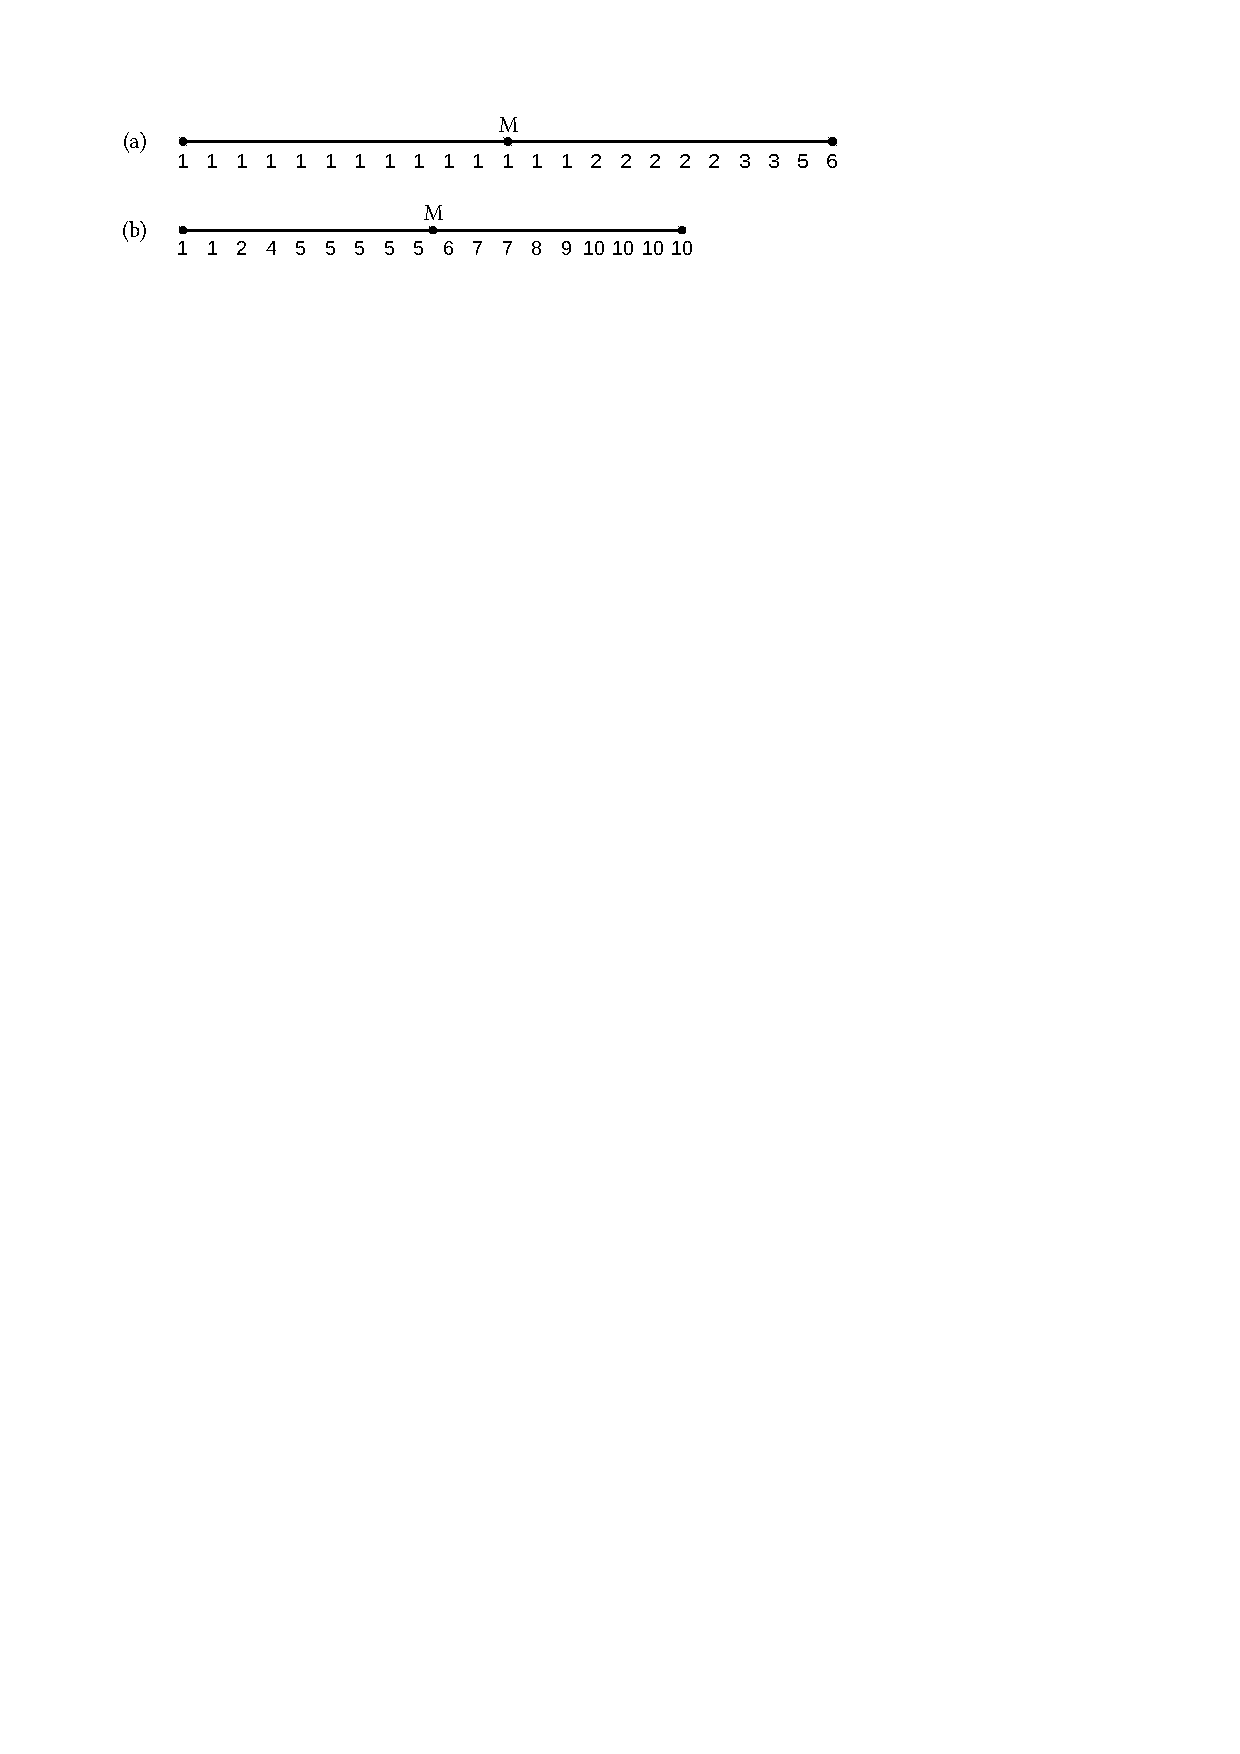
\includegraphics{figures/medians}
\end{figure}
% me: a) 1 1 1 1 1 1 1 1 1 1 1 \textbf{1} 1 1 2 2 2 2 2 3 3 5 6
% me: b) 1 1 2 4 5 5 5 5 \textbf{5 6} 7 7 8 9 10 10 10 10

If the sample consists of an even number of data points, we simply calculate the mean \is{mean} between the two values that lie in the middle of the ordered data set. For example, the rank values for the Animacy \is{animacy} of our sample of \textit{of}-possessives \is{possessive} are shown in Figure \ref{fig:possmedians}b. There are 18 values, so the median \is{median} falls between the ninth and the tenth value (marked again by a dot labeled M). The ninth and tenth value are 5 and 6 respectively, so the median for the \textit{of}-possessive modifiers is $\nicefrac{(5+6)}{2} = 5.5$ (i.e., it falls between \textvv{concrete touchable} and \textvv{concrete nontouchable}).

Using the idea of a median, \is{median} we can now rephrase our prediction in quantitative \is{quantitative research} terms:

\begin{exe}
\ex Prediction: The modifiers of the \textvv{\textit{s}-possessive} \is{possessive} will have a higher median on the \textvv{Animacy} \is{animacy} scale than the modifiers of the \textvv{\textit{of}-possessive}.
\label{ex:animacypredictionrank}
\end{exe}

Our data conform to this prediction, as 1 is higher on the scale than 5.5. As before, this does not prove or disprove anything, as, again, we would expect some random \is{chance} variation. \is{variation} Again, we will return to this issue in Chapter \ref{ch:significancetesting}.

\subsection{Frequency lists and mode}
\label{sec:mode}

Recall that I mentioned above the possibility of treating ordinal \is{ordinal data} data like nominal \is{nominal data} data. Table \ref{tab:relfreqpossmod} shows the relative frequencies \is{frequency} for each animacy \is{animacy} category, (alternatively, we could also calculate expected \is{frequency, expected} frequencies in the way described in Section \ref{sec:descriptiveordinal} above).

\begin{table}[!htbp]
\caption{Relative frequencies for the Animacy values of possessive modifiers}
\label{tab:relfreqpossmod}
\begin{tabular}[t]{rlcccc}
\lsptoprule
\multicolumn{2}{l}{\textvv{Animacy}} & \multicolumn{2}{c}{\textvv{\textit{s}-possessive}} & \multicolumn{2}{c}{\textvv{\textit{of}-possessive}} \\
Rank & Category & Abs. & Rel. & Abs. & Rel. \\
\midrule
1 & \textvv{human} & 14 & 0.609 & 2 & 0.111 \\
2 & \textvv{organization} & 5 & 0.217 & 1 & 0.056 \\
3 & \textvv{other animate} & 2 & 0.087 & 0 & -- \\
4 & \textvv{human attribute} & 0 & -- & 1 & 0.056 \\
5 & \textvv{concrete touchable} & 1 & 0.043 & 5 & 0.279 \\
6 & \textvv{concrete nontouchable} & 1 & 0.043 & 1 & 0.056 \\
7 & \textvv{location} & 0 & -- & 1 & 0.056 \\
8 & \textvv{time} & 0 & -- & 1 & 0.056 \\
9 & \textvv{event} & 0 & -- & 2 & 0.111 \\
10 & \textvv{abstract} & 0 & -- & 4 & 0.222 \\
\midrule
\multicolumn{2}{l}{Total} & 23 & 1.000 & 18 & 1.000 \\
\lspbottomrule
\end{tabular}
\end{table}

This table also nicely shows the preference of the \textit{s}-possessive \is{possessive} for animate \is{animacy} modifiers (human, organization, other animate) and the preference of the \textit{of}-possessive for the categories \is{categorization} lower on the hierarchy. The table also shows, however, that the modifiers of the \textit{of}-possessive are much more evenly distributed \is{distribution, conditional} across the entire \textvv{Animacy} \is{animacy} scale than those of the \textit{s}-possessive.

For completeness' sake, let me point out that there is a third measure of central tendency, that is especially suited to nominal \is{nominal data} data (but can also be applied to ordinal \is{ordinal data} and cardinal \is{cardinal data} data): the \textit{mode}. \is{mode} The mode is simply the most frequent value in a sample, so the modifiers of the \textit{of}-possessive \is{possessive} have a mode of 5 (or \textvv{concrete touchable}) and those of the \textit{s}-possessive have a mode of 1 (or \textvv{human}) with respect to animacy \is{animacy} (similarly, we could have said that the mode of \textit{s}-possessive modifiers is \textvv{discourse\hyp{}old} and the mode of \textit{of}-possessive modifiers is \textvv{discourse\hyp{}new}). There may be more than one mode \is{mode} in a given sample. For example, if we had found just a single additional modifier of the type \textvv{abstract} in the sample above (which could easily have happened), its frequency \is{frequency} would also be five; in this case, the \textit{of}-possessive \is{possessive} modifier would have two modes (\textvv{concrete touchable} and \textvv{abstract}). \is{animacy}

The concept of \textit{mode} \is{mode} may seem useful in cases where we are looking for a single value by which to characterize a set of nominal \is{nominal data} data, but on closer inspection it turns out that it does not actually tell us very much: it tells us what the most frequent value is, but it does not tell us how much more frequent that value is than the next most frequent one, how many other values occur in the data at all, etc. Thus, it is always preferable to report the frequencies \is{frequency} of all values, and, in fact, I have never come across a corpus\hyp{}linguistic study reporting modes. \is{mode}

\section{Descriptive statistics for cardinal data}
\label{sec:descriptivecardinal}

Let us turn, finally, to a design \is{research design} with one nominal \is{nominal data} and one cardinal \is{cardinal data} variable: a test of the third of the three hypotheses \is{hypothesis} introduced at the beginning of this chapter. Again, it is restated here together with the background assumption from which it is derived:

\begin{exe}
\ex Assumption: Short items tend to occur toward the beginning of a constiutent, long items tend to occur at the end. \\
Hypothesis: \is{hypothesis} The \textvv{\textit{s}-possessive} \is{possessive} will be used with short modifiers, the \textvv{\textit{of}-possessive} will be used with long modifiers.
\label{ex:lengthhypothesis}
\end{exe}

The constructions are operationalized \is{operationalization} as before. The data used are based on the same data set as before, except that cases with proper names and pronouns \is{pronoun} are excluded. The reason for this is that we already know from the first case study that pronouns, which we used as an operational definition of ``old information'' prefer the \textit{s}-possessive. \is{possessive} Since all pronouns are very short (regardless of whether we measure \is{measurement} their length \is{length} in terms of words, syllables \is{syllable} or letters), including them would bias our data in favor of the hypothesis. \is{hypothesis} This left 20 cases of the \textit{s}-possessive and 154 cases of the \textit{of}-possessive. To get samples \is{sampling} of roughly equal size \is{corpus size} for expository clarity, let us select every sixth case of the \textit{of}-possessive, \is{possessive} giving us 25 cases (note that in a real study, there would be no good reason to create such roughly equal sample sizes \is{corpus size} -- we would simply use all the data we have).

The variable \textvv{Length} \is{length} was defined operationally \is{operationalization} as ``number of orthographic words''. We can now state the following prediction:

\begin{exe}
\ex Prediction: The mean length of modifiers of the \textvv{\textit{s}-possessive} should be smaller than that of the modifiers of the \textvv{\textit{of}-possessive}.
\label{ex:lengthprediction}
\end{exe}

Table \ref{tab:samplelengthsgenofc} shows the length of head and modifier for all cases in our sample.

\begin{table}[!htbp]
\caption{A sample of \textit{s}- and \textit{of}-possessives annotated for length of head and modifier (BROWN)}
\label{tab:samplelengthsgenofc}
\resizebox*{!}{\textheight}{
\begin{tabular}[t]{rlrr}
\lsptoprule
No. & Example & Modifier & Head \\
\midrule
(a) & \multicolumn{3}{l}{\textvv{\textit{s}-possessive}} \\
\midrule
1 & \makecell[lt]{\textit{the government's special ceremonies at Memorial University} \\ \textit{honoring distinguished sons and daughters of the island province}} & 2 & 14 \\
2 & \textit{the year's grist of nearly 15,000 book titles} & 2 & 6 \\
3 & \textit{a burgomaster's Beethoven} & 2 & 1 \\
4 & \textit{the world's finest fall coloring} & 2 & 3 \\
5 & \textit{a standard internist's text} & 3 & 1 \\
6 & \textit{mom's apple pie} & 1 & 2 \\
7 & \textit{the Square's historic value} & 2 & 2 \\
8 & \textit{his mother's urging} & 2 & 1 \\
9 & \textit{the Department's recommendation} & 2 & 1 \\
10 & \textit{the posse's approach} & 2 & 1 \\
11 & \textit{ladies' fashions} & 1 & 1 \\
12 & \textit{the convict's climactic reappearance in London} & 2 & 4 \\
13 & \textit{industry's main criticism of the Navy's antisubmarine effort} & 1 & 7 \\
14 & \textit{the town marshal's office} & 3 & 1 \\
15 & \textit{the pool's edge} & 2 & 1 \\
16 & \textit{man's tongue} & 1 & 1 \\
17 & \textit{an egotist's rage for fame} & 2 & 3 \\
18 & \textit{a women's floor} & 2 & 1 \\
19 & \textit{these shores' peculiar powers of stimulation} & 2 & 4 \\
20 & \textit{the novelist's carping phrase} & 2 & 2 \\
\midrule
(b) & \multicolumn{3}{l}{\textvv{\textit{of}-possessive}} \\
\midrule
 1 & \textit{the announcement last week of the forthcoming encounter} & 3 & 4 \\
 2 & \textit{the necessity of interpretation by a Biblical scholar} & 5 & 2 \\
 3 & \textit{his portrayal of an edgy head\hyp{}in\hyp{}the\hyp{}clouds artist} & 4 & 2 \\
 4 & \textit{a lack of unity of purpose and respect for heroic leadership} & 8 & 2 \\
 5 & \textit{the death throes of men who were shot before the paredon} & 7 & 3 \\
 6 & \textit{lack of rainfall} & 1 & 1 \\
 7 & \makecell[lt]{\textit{the amazing variety and power of reactions, attitudes,} \\ \textit{and emotions precipitated by the nude form}} & 9 & 5 \\
 8 & \textit{the wet end of the cork} & 2 & 3 \\
 9 & \textit{the constitution of his home state of Massachusetts} & 5 & 2 \\
10 & \textit{the spirit of the mad genius from Baker Street} & 6 & 2 \\
11 & \textit{Ann's own description of the scene} & 2 & 3 \\
12 & \textit{considerable criticism of its length} & 2 & 2 \\
13 & \textit{the exaltations of combat} & 1 & 2 \\
14 & \textit{the existence of Prandtl numbers reaching values of more than unity} & 8 & 2 \\
15 & \textit{the outstanding standard bearer of Mr. Brown's tradition for accuracy} & 5 & 4 \\
16 & \textit{the growth of senile individuals} & 2 & 2 \\
17 & \textit{the totality of singular lines} & 2 & 2 \\
18 & \makecell[lt]{\textit{a consequence of the severe condition of perceived threat that persists } \\ \textit{unabated for the anxious child in an ambiguous sort of school environment}} & 20 & 2 \\
19 & \textit{the lead of the Russians} & 2 & 2 \\
20 & \textit{costs of service} & 1 & 1 \\
21 & \textit{ineffective dispersion of stock ownership} & 2 & 2 \\
22 & \textit{the value of a for the major portion of the knife} & 8 & 2 \\
23 & \textit{the eyes of the Lord's servants} & 3 & 2 \\
24 & \textit{the high ridge of the mountains} & 2 & 3 \\
25 & \textit{the pirouette of his arms} & 2 & 2 \\
\lspbottomrule
\end{tabular}}
\end{table}

\subsection{Means}
\label{sec:means}

How to calculate a mean \is{mean} (more precisely, an arithmetic mean) should be common knowledge, but for completeness' sake, the formula is given in (\ref{ex:formulamean}):

\begin{exe}
\ex $\displaystyle{\overline{x}_{arithm} = \frac{1}{n}\sum _{i=1}^nx_i = \frac{x_1+x_2+...+x_n}{n}}$
\label{ex:formulamean}
\end{exe}

In other words, in order to calculate the mean \is{mean} of a set of values $x_1, x_2, ..., x_n$ of size n, we add up all values and divide them by \textit{n} (or multiply them by $\nicefrac{1}{n}$, which is the same thing).

Since we have stated our hypothesis \is{hypothesis} and the corresponding prediction only in terms of the modifier, we should first make sure that the heads of the two possessives \is{possessive} do not differ greatly in length: \is{length} if they did, any differences we find for the modifiers could simply be related to the fact that one of the constructions may be longer in general than the other. Adding up all 20 values for the \textit{s}-possessive heads gives us a total of 57, so the mean \is{mean} is $\nicefrac{57}{20} = 2.85$. Adding up all 25 values of the \textit{of}-possessive heads gives us a total of 59, so the mean is $\nicefrac{59}{25} = 2.36$. We have, as yet, no way of telling whether this difference could be due to chance, \is{chance} but the two values are so close together that we will assume so for now. In fact, note that there is one obvious outlier (a value that is much bigger than the others: example (a 1) in Table \ref{tab:samplelengthsgenofc} has a head that is 14 words long. If we assume that this is somehow exceptional and remove this value, we get a mean \is{mean} length \is{length} of $\nicefrac{43}{19} = 2.26$, which is almost identical to the mean length of the \textit{of}-possessive's \is{possessive} modifiers.

If we apply the same formula to the modifiers, however, we find that they differ substantially: the mean \is{mean} length \is{length} of the \textit{s}-possessive \is{possessive} modifiers is $\nicefrac{38}{20} = 1.9$, while the mean length of the \textit{of}-possessive's modifiers is more than twice as much, namely $\nicefrac{112}{25} = 4.48$. Even if we remove the obvious outlier, example (b 18) in Table \ref{tab:samplelengthsgenofc}, the \textit{of}-possessive's modifiers are twice as long as those of the \textit{s}-possessive, namely $\nicefrac{92}{24} = 3.83$.

\section{Summary}
\label{sec:datatypessummary}

We have looked at three case studies, one involving nominal, \is{nominal data} one ordinal \is{ordinal data} and one cardinal \is{cardinal data} data. In each case, we were able to state a hypothesis \is{hypothesis} and derive a quantitative \is{quantitative research} prediction from it. Using appropriate descriptive \is{description} statistics \is{statistics} (percentages, observed and expected \is{frequency, expected} frequencies, modes, \is{mode} medians \is{median} and means \is{mean}), we were able to determine that the data conform to these predictions -- i.e., that the quantitative distribution \is{distribution, conditional} of the values of the variables \textvv{Givenness} \is{givenness} (measured \is{measurement} by \textvv{Part of Speech}, \textvv{Animacy} and \textvv{Length} \is{length} across the conditions \textvv{\textit{s}-possessive} \is{possessive} and \textvv{\textit{of}-possessive} fits the predictions formulated.

However, these distributions \is{distribution, conditional} by themselves do not prove (or, more precisely, \textit{fail to disprove}) the hypotheses \is{hypothesis} for two related reasons. First, the predictions are stated in relative terms, i.e. in terms of more\hyp{}or\hyp{}less, but they do not tell us \textit{how much} more or less we should expect to observe. Second, we do not know, and currently have no way of determining, whether the more\hyp{}or\hyp{}less that we observe reflects real differences in distribution, \is{distribution, conditional} or whether it falls within the range of random \is{chance} variation \is{variation} that we always expect when observing tendencies. More generally, we do not know how to apply the Popperian all\hyp{}or\hyp{}nothing research logic to quantitative \is{quantitative research} predictions. All this will be the topic of the next chapter.

\chapter{Significance testing}
\label{ch:significancetesting}

As discussed extensively in Chapter \ref{ch:scientificmethod}, scientific hypotheses \is{hypothesis} that are stated in terms of universal statements can only be falsified \is{falsification} (proven to be false), but never verified (proven to be true). This insight is the basis for the Popperian idea of a research cycle where the researcher formulates a hypothesis and then attempts to falsify it. If they manage to do so, the hypothesis has to be rejected and replaced by a new hypothesis. As long as they do not manage to do so, they may continue to treat it as a useful working hypothesis. \is{hypothesis} They may even take the repeated failure to falsify \is{falsification} a hypothesis as corroborating \is{corroboration} evidence for its correctness. If the hypothesis can be formulated in such a way that it could be falsified by a counterexample \is{counterexample} (and if it is clear what would count as a counterexample), this procedure seems fairly straightforward.

However, as also discussed in Chapter \ref{ch:scientificmethod}, many if not most hypotheses \is{hypothesis} in corpus linguistics have to be formulated in relative terms -- like those introduced in Chapter \ref{ch:quantifyingresearch}. As discussed in Section \ref{sec:testinghypotheses}, individual counterexamples \is{counterexample} are irrelevant in this case: if my hypothesis is that most swans are white, this does not preclude the existence of differently\hyp{}colored swans, so the hypothesis is not falsified \is{falsification} if we come across a black swan in the course of our investigation. In this chapter, we will discuss how relative statements can be investigated within the scientific framework introduced in Chapter \ref{ch:scientificmethod}.

\section{Statistical hypothesis testing}
\label{sec:statisticalhypothesistesting}

Obviously, if our hypothesis \is{hypothesis} is stated in terms of proportions rather than absolutes, we must also look at our data in terms of proportions rather than absolutes. A single counterexample \is{counterexample} will not disprove our hypothesis, but what if the majority cases we come across are counterexamples? For example, if we found more black swans than white swans, would this not falsify \is{falsification} our hypothesis that most swans are white? The answer is: not quite. With a hypothesis stated in absolute terms, it is easy to specify how many counterexamples \is{counterexample} we need to disprove it: one. If we find just one black swan, then it cannot be true that all swans are white, regardless of how many swans we have looked at and how many swans there are.

But with a hypothesis \is{hypothesis} stated in terms of proportions, matters are different: even if the majority or even all of the cases in our data contradict it, this does not preclude the possibility that our hypothesis is true -- our data will always just constitute a sample, \is{sampling} and there is no telling whether this sample corresponds to the totality of cases from which it was drawn. Even if most or all of the swans we observe are black, this may simply be an unfortunate accident -- in the total population of swans, the majority could still be white. (By the same reasoning, of course, a hypothesis is not verified if our sample consists exclusively of cases that corroborate \is{corroboration} it, since this does not preclude the possibility that in the total population, counterexamples \is{counterexample} are the majority).

So if relative statements cannot be falsified, \is{falsification} and if (like universal statements) they cannot be verified, what can we do? There are various answers to this question, all based in probability \is{probability} theory (i.e., statistics). \is{statistics} The most widely\hyp{}used and broadly\hyp{}accepted of these, and the one we adopt in this book, is an approach sometimes referred to as ``Null Hypothesis \is{null hypothesis} Significance Testing''.\footnote{It should be mentioned that there is a small but vocal group of critics that have pointed out a range of real and apparent problems with Null\hyp{}Hypothesis Significance Testing. In my view, there are three reasons that justify ignoring their criticism in a text book like this. First, they have not managed to convince a significant (pun intended) number of practitioners in any field using statistics, \is{statistics} which may not constitute a theoretical argument against the criticism, but certainly a practical one. Second, most, if not all of the criticisms, pertain to the way in which Null Hypothesis \is{null hypothesis} Significance Testing is used and to the way in which the results are (mis-)interpreted in the view of the critics. Along with many other practitioners, and even some of the critics, I believe that the best response to this is to make sure we apply the method appropriately and interpret the results carefully, rather than to give up a near\hyp{}universally used fruitful set of procedures. Third, it is not clear to me that the alternatives suggested by the critics are, on the whole, less problematic or less prone to abuse and misinterpretation.}

In this approach, which I will refer to simply as \textit{statistical hypothesis testing}, the problem of the non\hyp{}falsifiability \is{falsification} of quantitative \is{quantitative research} hypotheses is solved in an indirect but rather elegant way. Note that with respect to any two variables, there are two broad possibilities concerning their distribution \is{distribution, conditional} in a population: the distribution could be random \is{chance} (meaning that there is no relationship between the values of the two variables), or it could be non\hyp{}random \is{chance} (meaning that one value of one variable is more probable to occur with a particular value of the other variable). For example, it could be the case that swans are randomly \is{chance} black or white, or it could be the case that they are more probable to have one of these colors. If the latter is true, there are, again, two broad possibilities: the data could agree with our hypothesis, or they could disagree with it. For example, it could be the case that there are more white swans than black swans (corroborating \is{corroboration} our hypothesis), or that there are more black swans than white swans (falsifying \is{falsification} our hypothesis).

Unless we have a very specific prediction as to exactly what proportion of our data should consist of counterexamples, \is{counterexample} we cannot draw any conclusions from a sample. \is{sampling} For most research hypotheses, we cannot specify such an exact proportion -- if our hypothesis is that \textvv{Most swans are white}, then ``most'' could mean anything from 50.01 percent to 99.99 percent. But as we will see in the next subsection, we can always specify the exact proportion of counterexamples that we would expect to find if there was a \textit{random} \is{chance} relationship between our variables, and we can then use a sample whether such a random \is{chance} relationship holds (or rather, how probable it is to hold).

Statistical hypothesis testing utilizes this fact by formulating not one, but two hypotheses -- first, a research hypothesis postulating a relationship between two variables (like ``Most swans are white'' or like the hypotheses introduced in Chapter \ref{ch:quantifyingresearch}), also referred to as H\textsubscript{1} or ``alternative hypothesis''; second, the hypothesis that there is a random \is{chance} relationship between the variables mentioned in the research hypothesis, also referred to as H\textsubscript{0} or ``null hypothesis''. \is{null hypothesis} We then attempt to falsify \is{falsification} the \textit{null hypothesis} and to show that the data conform to the alternative hypothesis.

In a first step, this involves turning the null hypothesis \is{null hypothesis} and the alternative hypothesis are turned into quantitative \is{quantitative research} predictions concerning the intersections of the variables, as schematically shown in (\ref{ex:schematicnullalternative}a, b):

\begin{exe}
\ex
\begin{xlist}
\label{ex:schematicnullalternative}
\ex Null hypothesis \is{null hypothesis} (H\textsubscript{0}): There is no relationship between Variable A and Variable B. \\[2ex]
Prediction: The data should be distributed \is{distribution, conditional} randomly \is{chance} across the intersections of A and B; i.e., the frequency\slash medians\slash means \is{median} \is{mean} \is{frequency} of the intersections should not differ from those expected \is{frequency, expected} by chance. \is{chance}
\ex Alternative hypothesis (H\textsubscript{1}): There is a relationship between Variable A and Variable B such that some value(s) of A tend to co\hyp{}occur with some value(s) of B. \\[2ex]
Prediction: The data should be distributed \is{distribution, conditional} non\hyp{}randomly \is{chance} across the intersections of A and B; i.e., the frequency\slash medians\slash means \is{median} \is{mean} \is{frequency} of some the intersections should be higher and\slash or lower than those expected \is{frequency, expected} by chance. \is{chance}
\end{xlist}
\end{exe}

Once we have formulated our research hypothesis and the corresponding null hypothesis \is{null hypothesis} in this way (and once we have operationalized \is{operationalization} the constructs used in formulating them), we collect, annotate \is{annotation} and quantify \is{quantitative research} the relevant data, as discussed in the preceding chapter.

The crucial step in terms of statistical significance \is{significance} testing then consists in determining whether the observed distribution \is{distribution, conditional} differs from the distribution we would expect if the null hypothesis \is{null hypothesis} were true -- if the values of our variables were distributed randomly \is{chance} in the data. Of course, it is not enough to observe a difference -- a certain amount of variation \is{variation} is to be expected \is{frequency, expected} even if there is no relationship between our variables. As will be discussed in detail in the next section, we must determine whether the difference is large enough to assume that it does not fall within the range of variation that could occur randomly. \is{chance} If we are satisfied that this is the case, we can (provisionally) reject the null hypothesis. \is{null hypothesis} If not, we must (provisionally) reject our research hypothesis.

In a third step (or in parallel with the second step), we must determine whether the data conform to our research hypothesis, or, more precisely, whether they differ from the prediction of H\textsubscript{0} \textit{in the direction predicted by H\textsubscript{1}}. If they do (for example, if there are more white swans than black swans), we can (provisionally) accept our research hypothesis, i.e., we can continue to use it as a working hypothesis in the same way that we would continue to use an absolute hypothesis in this way as long as we do not find a counterexample. \is{counterexample} If the data differ from the prediction of H\textsubscript{0} in the \textit{opposite} direction to that predicted by our research hypothesis -- for example, if there are more black than white swans -- we must, of course, also reject our research hypothesis, and treat the unexpected result as a new problem to be investigated further.

Let us now turn to a more detailed discussion of probabilities, \is{probability} random \is{chance} variation \is{variation} and how statistics \is{statistics} can be used to (potentially) reject null hypotheses. \is{null hypothesis}

\section{Probabilities and significance testing}
\label{sec:probabilitysignificance}

Recall the example of a coin that is flipped onto a hard surface: every time we flip it, there is a fifty percent probability \is{probability} that it will come down heads, and a fifty percent probability that it will come down tails. From this it follows, for example, that if we flip a coin ten times, the expected \is{frequency, expected} outcome is five heads and five tails. However, as pointed out in the last chapter, this is only a theoretical expectation derived from the probabilities of each individual outcome. In reality, every outcome -- from ten heads to ten tails is \textit{possible}, as each flip of the coin is an independent event. \is{animacy}

Intuitively, we know this: if we flip a coin ten times, we do not really expect it to come down heads and tails exactly five times each but we accept a certain amount of variation. \is{variation} However, the greater the imbalance between heads and tails, the less willing we will be to accept it as a result of chance. \is{chance} In other words, we would not be surprised if the coin came down heads six times and tails four times, or even heads seven times and tails three times, but we might already be slightly surprised if it came down heads eight times and tails only twice, and we would certainly be surprised to get a series of ten heads and no tails.

Let us look at the reasons for this surprise, beginning with a much shorter series of just two coin flips. There are four possible outcomes of such a series:

\begin{exe}
\ex
\begin{xlist}
\label{ex:headstails}
\ex heads -- heads
\ex heads -- tails
\ex tails -- heads
\ex tails -- tails
\end{xlist}
\end{exe}

Obviously, none of these outcomes is more or less probable than the others: since there are four possible outcomes, they each have a probability \is{probability} of $\nicefrac{1}{4} = 0.25$ (i.e., 25 percent, we will be using the decimal notation for percentages from here on). Alternatively, we can calculate the probability of each series by multiplying the probability of the individual events \is{animacy} in each series, i.e. $0.5 \times 0.5 = 0.25$.

Crucially, however, there are differences in the probability \is{probability} of getting a particular \textit{set} of results (i.e, a particular number of heads and regardless of the order they occur in): There is only one possibility of getting two heads (\ref{ex:headstails}a) and one of getting two tails (\ref{ex:headstails}d), but there are two possibilities of getting one head and one tail ((\ref{ex:headstails}b, c). We calculate the probability of a particular set by adding up the probabilities \is{probability} of all possible series that will lead to this set. Thus, the probabilities for the sets \{heads, heads\} and \{tails, tails\} are 0.25 each, while the probability for the set \{heads, tails\}, corresponding to the series heads--tails and tails--heads, is 0.25 + 0.25 = 0.5.

This kind of coin\hyp{}flip logic (also known as probability \is{probability} theory), can be utilized in evaluating quantitative \is{quantitative research} hypotheses that have been stated in quantitative terms. Take the larger set of ten coin flips mentioned at the beginning of this section: now, there are eleven potential outcomes, shown in Table \ref{tab:tencoinflips}.

\begin{table}[!htbp]
\caption{Possible sets of ten coin flips}
\label{tab:tencoinflips}
\begin{tabular}[t]{rccc}
\lsptoprule & Unordered Set & No. of Series & Probability \\
\midrule
1 & \{0 heads, 10 tails\} & 1 & 0.000977 \\
2 & \{1 heads, 9 tails\} & 10 & 0.009766 \\
3 & \{2 heads, 8 tails\} & 45 & 0.043945 \\
4 & \{3 heads, 7 tails\} & 120 & 0.117188 \\
5 & \{4 heads, 6 tails\} & 210 & 0.205078 \\
6 & \{5 heads, 5 tails\} & 252 & 0.246094 \\
7 & \{6 heads, 4 tails\} & 210 & 0.205078 \\
8 & \{7 heads, 3 tails\} & 120 & 0.117188 \\
9 & \{8 heads, 2 tails\} & 45 & 0.043945 \\
10 & \{9 heads, 1 tails\} & 10 & 0.009766 \\
11 & \{10 heads, 0 tails\} & 1 & 0.000977 \\
\lspbottomrule
\end{tabular}
\end{table}

Again, these outcomes differ with respect to their probability. \is{probability} The third column of Table \ref{tab:tencoinflips} gives us the number of different series corresponding to each set.\footnote{You may remember having heard of Pascal's triangle, which, among more sophisticated things, lets us calculate the number of different ways in which we can get a particular combination of heads and tails for a given number of coin flips: the third column of Table \ref{tab:tencoinflips} corresponds to line 11 of this triangle. If you don't remember, no worries, we will not need it.} For example, there is only one way to get a set consisting of heads only: the coin must come down showing heads every single time. There are ten different ways of getting one heads and nine tails: The coin must come down heads the first or second or third or fourth or fifth or sixth or seventh or eighth or ninth or tenth time, and tails the rest of the time. Next, there are forty\hyp{}five different ways of getting two heads and eight tails, which I am not going to list here (but you may want to, as an exercise), and so on. The fourth column contains the same information, expressed in terms of relative frequencies: \is{frequency} there are 1024 different series of ten coin flips, so the probability \is{probability} of getting, for example, two heads and eight tails is $\nicefrac{45}{1024} = 0.043945$.

The basic idea behind statistical hypothesis testing is simple: we calculate the probability \is{probability} of the result that we have observed. The lower this probability is, the less likely it is to have come about by chance \is{chance} and the more probable is it that we will be right if we reject the null hypothesis. \is{null hypothesis} For example, if we observed a series of ten heads and zero tails, we know that the likelihood that the deviation from the expected \is{frequency, expected} result of five heads and five tails is due to chance \is{chance} is 0.000977 (i.e. roughly a tenth of a percent). This tenth of a percent is also the probability \is{probability} that we are wrong if we reject the null hypothesis and claim that the coin is not behaving randomly \is{chance} (for example, that it is manipulated in some way).

If we observed one heads and nine tails, we would know that the likelihood \is{probability} that this deviation from the expected \is{frequency, expected} result is 0.009766 (i.e. almost one percent). Thus we might think that, again, if we reject the null hypothesis, \is{null hypothesis} this is the probability \is{probability of error} that we are wrong. However, we must add to this the probability of getting ten heads and zero tails. The reason for this is that if we accept a result of 1:9 as evidence for a non\hyp{}random \is{chance} distribution, \is{distribution, conditional} we would also accept the even more extreme result of 0:10. So the probability that we are wrong in rejecting the null hypothesis is 0.000977 + 0.009766 = 0.010743. In other words: the probability that we are wrong in rejecting the null hypothesis \is{null hypothesis} is always the probability of the observed result plus the probabilities of all results that deviate from the null hypothesis even further in the direction of the observed frequency. \is{frequency, observed} \is{frequency} This is called the ``probability of error'' (or simply \textit{p}-value) \is{p-value} in statistics. \is{statistics}

It must be mentioned at this point that some researchers (especially opponents of null\hyp{}hypothesis statistical significance \is{significance} testing) disagree that \textit{p} can be interpreted as the probability \is{probability of error} that we are wrong in rejecting the null hypothesis, \is{null hypothesis} raising enough of a controversy to force the American Statistical Association to take an official stand on the meaning of \textit{p}: \is{p-value}

\begin{quote}
Informally, a p\hyp{}value \is{p-value} is the probability under a specified statistical model that a statistical summary of the data (e.g., the sample mean difference between two compared groups) would be equal to or more extreme than its observed value. \citep[131]{wasserstein_asas_2016}
\end{quote}

Although this is the informal version of their definition, it may be completely incomprehensible at first glance, but it is actually just a summary of the discussion above: the ``specified statistical model'' in our case is the null hypothesis, \is{null hypothesis} i.e., the hypothesis that our data have come about purely by chance. \is{chance} The p\hyp{}value \is{p-value} thus tells us how probable it is under this hypothesis that we would observe the result we have observed, or an even more extreme result.

It also tells us how likely we are wrong if we reject this null hypothesis: \is{null hypothesis} If our model (i.e. the null hypothesis) will occasionally produce our observed result (or a more extreme one), then we will be wrong in rejecting it at those occasions. The p\hyp{}value \is{p-value} tells us, how likely it is that we are dealing with such an occasion. Of course, it does \textit{not} tell us how likely it is that the null hypothesis is actually true or false -- we do not know this likelihood and we can never know it. Statistical hypotheses are no different in this respect from universal hypotheses. Even if we observe a result with a probability \is{probability} of one in a million, the null hypothesis \is{null hypothesis} could be true (as we might be dealing with this one\hyp{}in\hyp{}a\hyp{}million event), \is{animacy} and even if we observe a result with a probability of \num{999999} in a million, the null hypothesis could be false (as our result could nevertheless have come about by chance). \is{chance} The p\hyp{}value \is{p-value} simply tells us how likely it is that our study -- with all its potential faults, confounding variables, etc. -- would produce the result we observe and thus how likely we are wrong \textit{on the basis of this study} to reject the null hypothesis. \is{null hypothesis} This simply means that we should not start believing in our hypothesis until additional studies have rejected the null hypothesis -- an individual study may lead us to wrongly reject the null hypothesis, but the more studies we conduct that allow us to reject the null hypothesis, the more justified we are in treating them as corroborating \is{corroboration} our research hypothesis.

By convention, probability \is{probability of error} of error of 0.05 (five percent) is considered to be the limit as far as acceptable risks are concerned in statistics \is{statistics} -- if $p < 0.05$ (i.e., if \textit{p} is smaller than five percent), the result is said to be \textit{statistically significant} \is{significance} (i.e., not due to chance), \is{chance} if it is larger, the result is said to be non\hyp{}significant (i.e., likely due to chance). \is{chance} Table \ref{tab:plevels} \is{p-value} shows additional levels of significance that are conventionally recognized.

\begin{table}[!htbp]
\caption{Interpretation of p\hyp{}values}
\label{tab:plevels}
\begin{tabular}[t]{lc}
\lsptoprule
p\hyp{}value & Level of significance \\
\midrule
$\geq 0.05$ & not significant \\
$< 0.05$ & significant \\
$< 0.01$ & very significant \\
$< 0.001$ & highly significant \\
\lspbottomrule
\end{tabular}
\end{table}

Obviously, these cut\hyp{}off points are largely arbitrary (a point that is often criticized by opponents of null\hyp{}hypothesis significance \is{significance} testing): it is strange to be confident in rejecting a null hypothesis \is{null hypothesis} if the probability \is{probability of error} of being wrong in doing so is five percent, but to refuse to reject it if the probability of being wrong is six percent (or, as two psychologists \is{psychology} put it: ``Surely, God loves the .06 nearly as much as the .05'' \citep[1277]{rosnow_statistical_1989}).

In real life, of course, researchers do not treat these cut\hyp{}off points as absolute. Nobody would simply throw away a set of carefully collected data as soon as their calculations yielded a p\hyp{}value \is{p-value} of 0.06 or even 0.1. Some researchers actually report such results, calling p\hyp{}values between 0.05 and 0.10 ``marginally significant'', \is{significance} and although this is often frowned upon, there is nothing logically wrong with it. Even the majority of researchers who are unwilling to report such results would take them as an indicator that additional research might be in order (especially if there is a reasonable effect size, \is{effect size} see further below).

They might re\hyp{}check their operational \is{operationalization} definitions and the way they were applied, they might collect additional data in order to see whether a larger data set yields a lower probability \is{probability of error} of error, or they might replicate \is{replicability} the study with a different data set. Note that this is perfectly legitimate, and completely in line with the research cycle sketched out in Section \ref{sec:researchcycle} -- provided we retain all of our data. What we must not do, of course, is test different data sets until we find one that gives us a significant \is{significance} result, and then report just that result, ignoring all attempts that did not yield significant results. What we must also not do is collect an extremely large \is{corpus size} data set and then keep drawing samples \is{sampling} from it until we happen to draw one that gives us a significant result. These practices are sometimes referred to as \textit{p\hyp{}hacking}, and they constitute a scientific fraud (imagine a a researcher who wants to corroborate \is{corroboration} their hypothesis that all swans are white and does so by simply ignoring all black swans they find).

Clearly, what probability \is{probability of error} of error one is willing to accept for any given study also depends on the nature of the study, the nature of the research design, \is{research design} and a general disposition to take or avoid risk. If mistakenly rejecting the null hypothesis \is{null hypothesis} were to endanger lives (for example, in a study of potential side\hyp{}effects of a medical treatment), we might not be willing to accept a p\hyp{}value \is{p-value} of 0.05 or even 0.01.

Why would collecting additional data be a useful strategy, or, more generally speaking, why are corpus\hyp{}linguists (and other scientists) often intent on making their samples as large as possible and\slash or feasible? Note that the probability \is{probability of error} of error depends not just on the proportion of the deviation, but also on the overall size \is{corpus size} of the sample. For example, if we observe a series of two heads and eight tails (i.e., twenty percent heads), the probability of error in rejecting the null hypothesis \is{null hypothesis} is $0.000977 + 0.009766 + 0.043945 = 0.054688$. However, if we observe a series of four heads and sixteen tails (again, twenty percent heads), the probability \is{probability of error} of error would be roughly ten times lower, namely 0.005909. The reason is the following: There are \num{1048576} possible series of twenty coin flips. There is still only one way of getting one head and nineteen tails, so the probability of getting one head and nineteen tails is $\nicefrac{1}{1048576} = 0.0000009536743$; however, there are already 20 ways of getting one tail and nineteen heads (so the probability is $\nicefrac{20}{1048576} = 0.000019$), 190 ways of getting two heads and eighteen tails ($p = \nicefrac{190}{1048576} = 0.000181$), 1140 ways of getting three heads and seventeen tails ($p = \nicefrac{1140}{1048576} = 0.001087$) and 4845 ways of getting four heads and sixteen tails ($p = \nicefrac{4845}{1048576} = 0.004621$). And adding up these probabilities gives us 0.005909.

Most research designs \is{research design} in any discipline are more complicated than coin flipping, which involves just a single variable with two values. However, it is theoretically possible to generalize the coin\hyp{}flipping logic to any research design, i.e., calculate the probabilities \is{probability} of all possible outcomes and add up the probabilities of the observed outcome and all outcomes that deviate from the expected \is{frequency, expected} outcome even further in the same direction. Most of the time, however, this is only a theoretical possibility, as the computations quickly become too complex to be performed in a reasonable time frame even by supercomputers, let alone by a standard\hyp{}issue home computer or manually.

Therefore, many statistical methods use a kind of mathematical detour: they derive from the data a single value whose probability distribution \is{distribution, conditional} is known -- a so\hyp{}called \textit{test statistic}. Instead of calculating the probability \is{probability} of our observed outcome directly, we can then assess its probability by comparing the test statistic against its known distribution. Mathematically, this involves identifying its position on the respective distribution and, as we did above, adding up the probability of this position and all positions deviating further from a random \is{chance} distribution. \is{distribution, conditional} In practice, we just have to look up the test statistic \is{statistics} in a chart that will give us the corresponding probability \is{probability} of error (or \textit{p}-value, as we will call it from now on).

In the following three sections, I will introduce three widely\hyp{}used tests involving test statistics for the three types of data discussed in the previous section: the chi\hyp{}square ($\chi^2$) \is{chi-square test} test for nominal \is{nominal data} data, the Wilcoxon\hyp{}Mann\hyp{}Whitney \is{Mann-Whitney U test} test (also known as Mann\hyp{}Whitney U test or Wilcoxon rank sum test) for ordinal \is{ordinal data} data, and Welch's t\hyp{}test \is{t-test} for cardinal \is{cardinal data} data. I will also briefly discuss extensions of the $\chi^2$ test for more complex research designs, \is{research design} including those involving more than two variables.

Given the vast range of corpus\hyp{}linguistic research designs, \is{research design} these three tests will not always be the ideal choice. In many cases, there are more sophisticated statistical procedures which are better suited to the task at hand, be it for theoretical (mathematical or linguistic) or for practical reasons. However, the statistical tests introduced here have some advantages that make them ideal procedures for an initial statistical evaluation of results. For example, they are easy to perform: we don't need more than a paper and a pencil, or a calculator, if we want to speed up things, and they are also included as standard functions in widely\hyp{}used spreadsheet applications. They are also relatively robust in situations where we should not really use them (a point I will return to below).

They are also ideal procedures for introducing statistics \is{statistics} to novices. Again, they are easy to perform and do not require statistical software packages that are typically expensive and\slash or have a steep learning curve. They are also relatively transparent with respect to their underlying logic and the steps required to perform them. Thus, my purpose in introducing them in some detail here is at least as much to introduce the logic and the challenges of statistical analysis, as it is to provide basic tools for actual research.

I will not introduce the mathematical underpinnings of these tests, and I will mention alternative and\slash or more advanced procedures only in passing -- this includes, at least for now, research designs \is{research design} where neither variable is nominal. \is{nominal data} In these cases, correlation \is{correlation} tests are used, such as Pearson's product\hyp{}moment correlations (if are dealing with two cardinal \is{cardinal data} variables) and Spearman's rank correlation coefficient or the Kendall tau rank correlation coefficient (if one or both of our variables are ordinal). \is{ordinal data}

I will not, in other words, do much more than scratch the surface of the vast discipline of statistics. \is{statistics} In the Study Notes to this chapter, there are a number of suggestions for further reading that are useful for anyone interested in a deeper understanding of the issues introduced here, and obligatory for anyone serious about using statistical methods in their own research. While I will not be making reference to any statistical software applications, such applications are necessary for serious quantitative \is{quantitative research} research; again, the Study Notes contain useful suggestions where to look.

\section{Nominal data: The chi\hyp{}square test}
\label{sec:chisquaretest}

As mentioned in the preceding chapter, nominal \is{nominal data} data (or data that are best treated like nominal data) are the type of data most frequently encountered in corpus linguistics. I will therefore treat them in slightly more detail than the other two types, introducing different versions and (in the next chapter) extensions of the most widely used statistical test for nominal \is{nominal data} data, the \textit{chi\hyp{}square} \is{chi-square test} ($\chi^2$) \textit{test}. This test in all its variants is extremely flexible; it is thus more useful across different research designs \is{research design} than many of the more specific and more sophisticated procedures (much like a Swiss army knife is an excellent all\hyp{}purpose tool despite the fact that there is usually a better tool dedicated to a specific task at hand).

Despite its flexibility, there are two requirements that must be met in order for the $\chi^2$ \is{chi-square test} test to be applicable: first, no intersection of variables must have a frequency \is{frequency} of zero in the data, and second, no more than twenty\hyp{}five percent of the intersections must have frequencies lower than five. When these conditions are not met, an alternative test must be used instead (or we need to collect additional data).

\subsection{Two\hyp{}by\hyp{}two designs}
\label{sec:chisquaretwobytwo}

Let us begin with a two\hyp{}by\hyp{}two design \is{research design} and return to the case of discourse\hyp{}old and discourse\hyp{}new modifiers in the two English possessive \is{possessive} constructions. Here is the research hypothesis again, paraphrased from (\ref{ex:givennesshypothesis}) and (\ref{ex:givennessprediction}) in Chapter \ref{ch:quantifyingresearch}:

\begin{exe}
\ex H\textsubscript{1}: There is a relationship between \textvv{Discourse Status} and \textvv{Type of Possessive} such that the \textvv{\textit{s}-possessive} is preferred when the modifier is \textvv{discourse\hyp{}old}, the \textvv{\textit{of}-possessive} \is{possessive} is preferred when the modifier is \textvv{discouse\hyp{}new}.\\[2ex]
Prediction: There will be more cases of the \textvv{\textit{s}-possessive} with \textvv{discourse\hyp{}old} modifiers than with \textvv{discourse\hyp{}new} modifiers, and more cases of the \textvv{\textit{of}-possessive} with discourse\hyp{}new modifiers than with \textvv{discourse\hyp{}old} modifiers.
\label{ex:givennessalternative}
\end{exe}

The corresponding null hypothesis \is{null hypothesis} is stated in (\ref{ex:givennessnull}): \is{givenness}

\begin{exe}
\ex H\textsubscript{0}: There is no relationship between \textvv{Discourse Status} and \textvv{Type of Possessive}.\\[2ex]
Prediction: Discourse\hyp{}old and discourse\hyp{}new modifiers will be distributed \is{distribution, conditional} randomly \is{chance} across the two Possessive \is{possessive} constructions.
\label{ex:givennessnull}
\end{exe}

We already reported the observed and expected \is{frequency, expected} frequencies in Table \ref{tab:obsexpfreqposs}, but let us repeat them here as Table \ref{tab:obsexpfreqpossrepeat} for convenience in a slightly simplified form that we will be using from now on, with the expected frequencies shown in parentheses below the observed ones.

% layout: In contingency tables like the following one, please do NOT align the numbers at the decimal point, they are intentionally formatted in this way.
\begin{table}[!htbp]
\caption{Observed and expected frequencies of old and new modifiers in the \textit{s}- and the \textit{of}-possessive (= Table \ref{tab:obsexpfreqposs})}
\label{tab:obsexpfreqpossrepeat}
\begin{tabular}[t]{llccr}
\lsptoprule
 & & \multicolumn{2}{c}{\textvv{Possessive}} & \\
 & & \textvv{\textit{s}-possessive} & \textvv{\textit{of}-possessive} & Total \\
\midrule
\textvv{\makecell[lt]{Discourse \\Status}} & \textvv{old} & \makecell[t]{180\\(102.81)} & \makecell[t]{3\\(80.19)} & \makecell[t]{183\\} \\
 & \textvv{new} & \makecell[t]{20\\(97.19)} & \makecell[t]{153\\(75.81)} & \makecell[t]{173\\} \\
\midrule
 & Total & \makecell[t]{200} & \makecell[t]{156} & \makecell[t]{356} \\
\lspbottomrule
\end{tabular}
\end{table}

In order to test our research hypothesis, we must show that the observed frequencies \is{frequency, observed} differ from the null hypothesis \is{null hypothesis} in the direction of our prediction. We already saw in Chapter \ref{ch:quantifyingresearch} that this is the case: The null hypothesis predicts the expected \is{frequency, expected} frequencies, but there are more cases of \textit{s}-possessives \is{possessive} with old modifiers and \textit{of}-possessives with new modifiers than expected. Next, we must apply the coin\hyp{}flip logic and ask the question: ``Given the sample size, how surprising is the difference between the expected frequencies (i.e., a perfectly random \is{chance} distribution) \is{distribution, conditional} and the observed frequencies \is{frequency, observed} (i.e., the distribution we actually find in our data)?''

As mentioned above, the conceptually simplest way of doing this would be to compute all possible ways in which the marginal frequencies (the sums of the columns and rows) could be distributed \is{distribution, conditional} across the four cells of our table and then check what proportion of these tables deviates from a perfectly random \is{chance} distribution at least as much as the table we have actually observed. For two\hyp{}by\hyp{}two tables, there is, in fact, a test that does this, the exact test \is{Fisher's exact test} (also called Fisher's exact test or, occasionally, Fisher\hyp{}Yates exact test), and where the conditions for using the $\chi^2$ \is{chi-square test} test are not met, we should use it. But, as mentioned above, this test is difficult to perform without statistical software, and it is not available for tables larger \is{corpus size} than 2\hyp{}by\hyp{}2 anyway, so instead we will derive the $\chi^2$ test statistic from the table.

First, we need to assess the magnitude of the differences between observed and expected \is{frequency, expected} frequencies. The simplest way of doing this would be to subtract the expected differences from the observed ones, giving us numbers that show for each cell the size \is{corpus size} of the deviation as well as its direction (i.e., are the observed frequencies \is{frequency, observed} higher or lower than the expected ones). For example, the values for Table \ref{tab:obsexpfreqpossrepeat} \is{possessive} would be 77.19 for cell C\textsubscript{11} (\textvv{\textit{s}-possessive} $\cap$ \textvv{old}), -77.19 for C\textsubscript{21} (\textvv{\textit{of}-possessive} $\cap$ \textvv{old}), -77.19 for C\textsubscript{12} (\textvv{\textit{s}-possessive} $\cap$ \textvv{new}) and 77.19 for C\textsubscript{22} (\textvv{\textit{of}-possessive} $\cap$ \textvv{new}).

However, we want to derive a single measure from the table, so we need a measure of the overall deviation of the observed frequencies \is{frequency, observed} from the expected, \is{frequency, expected} not just a measure for the individual intersections. Obviously, adding up the differences of all intersections does not give us such a measure, \is{measurement} as it would always be zero (since the marginal frequencies are fixed, any positive deviance in one cell will have a corresponding negative deviance in its neighboring cells). Second, subtracting the observed from the expected \is{frequency, expected} frequencies gives us the same number for each cell, when it is obvious that the actual magnitude of the deviation depends on the expected frequency. For example, a deviation of 77.19 is more substantial if the expected frequency is 75.81 than if the expected frequency is 102.81. In the first case, the observed frequency \is{frequency, observed} is more than a hundred percent higher than expected, in the second case, it is only 75 percent higher.

The first problem is solved by squaring the differences. This converts all deviations into positive numbers, and thus their sum will no longer be zero, and it has the additional effect of weighing larger deviations more strongly than smaller ones. The second problem is solved by dividing the squared difference by the expected \is{frequency, expected} frequencies. This will ensure that a deviation of a particular size will be weighed more heavily for a small expected frequency than for a large expected frequency. The values arrived at in this way are referred to as the \textit{cell components of $\chi^2$} \is{chi-square test} (or simply \textit{$\chi^2$ components}); the formulas for calculating the cell components in this way are shown in Table \ref{tab:formulachisquarecomp}.

\begin{table}[!htbp]
\caption{Calculating $\chi^2$ components for individual cells}
\label{tab:formulachisquarecomp}
\begin{tabular}[t]{llcc}
\lsptoprule
 & & \multicolumn{2}{c}{\textvv{Dependent Variable}} \\
 & & \textvv{value 1} & \textvv{value 2} \\
\midrule
\textvv{\textvv{\makecell[lt]{Independent \\Variable}}}
	& \textvv{value 1}
		& \makecell[c]{$\displaystyle{\frac{(O_{11} - E_{11})^2}{E_{11}}}$}
		& \makecell[c]{$\displaystyle{\frac{(O_{12} - E_{12})^2}{E_{12}}}$} \\
	& \textvv{value 2}
		& \makecell[c]{$\displaystyle{\frac{(O_{21} - E_{21})^2}{E_{21}}}$}
		& \makecell[c]{$\displaystyle{\frac{(O_{22} - E_{22})^2}{E_{22}}}$} \\
\lspbottomrule
\end{tabular}
\end{table}

If we apply this procedure to Table \ref{tab:obsexpfreqpossrepeat}, we get the components shown in Table \ref{tab:posschisquarecomp}.

\begin{table}[!htbp]
\caption{$\chi^2$ components for Table \ref{tab:obsexpfreqpossrepeat}}
\label{tab:posschisquarecomp}
\begin{tabular}[t]{llcc}
\lsptoprule
 & & \multicolumn{2}{c}{\textvv{Possessive}} \\
 & & \textvv{\textit{s}-possessive} & \textvv{\textit{of}-possessive} \\
\midrule
\textvv{\textvv{\makecell[lt]{Discourse \\Status}}}
	& \textvv{old}
		& \makecell[c]{$\frac{(180 - 102.81)^2}{102.81} = 57.96$}
		& \makecell[c]{$\frac{(3 - 80.19)^2}{80.19} = 74.3$} \\
	& \textvv{new}
		& \makecell[c]{$\frac{(20 - 97.19)^2}{97.19} = 61.31$}
		& \makecell[c]{$\frac{(153 - 75.81)^2}{75.81} = 78.6$} \\
\lspbottomrule
\end{tabular}
\end{table}

The degree of deviance from the expected \is{frequency, expected} frequencies for the entire table can then be calculated by adding up the $\chi^2$ \is{chi-square test} components. For Table 7.3, the $\chi^2$ value ($\chi^2$) is 272.16. This value can now be used to determine the probability \is{probability of error} of error by checking it against a table like that in Section \ref{sec:chisquarecriticalvalues} in the Statistical Tables at the end of this book.

Before we can do so, there is a final technical point to make. Note that the degree of variation \is{variation} in a given table that is expected \is{frequency, expected} to occur by chance \is{chance} depends quite heavily on the size of the table. The bigger the table, the higher the number of cells that can vary independently of other cells without changing the marginal sums (i.e., without changing the overall distribution). \is{distribution, conditional} The number of such cells that a table contains is referred to as the number of \textit{degrees of freedom} of the table. In the case of a two\hyp{}by\hyp{}two table, there is just one such cell: if we change any single cell, we must automatically adjust the other three cells in order to keep the marginal sums constant. Thus, a two\hyp{}by\hyp{}two table has one degree of freedom.

The general formula for determining the degrees of freedom of a table is the following, where $N_rows$ is the number of rows and $N_column$ is the number of columns:

\begin{exe}
\ex $\displaystyle{df = (N_{Rows} - 1) \times (N_{Columns} - 1)}$
\label{ex:formuladf}
\end{exe}

Significance levels of $\chi^2$ \is{chi-square test} values differ depending on how many degrees of freedom a table has, so we always need to determine the degrees of freedom before we can determine the p\hyp{}value. Turning to the table of $\chi^2$ values in Section \ref{sec:chisquarecriticalvalues}, \is{chi-square test} we first find the row for one degree of freedom (this is the first row); we then check whether our $\chi^2$-value is larger than that required for the level of significance \is{significance} that we are after. In our case, the value of 272.16 is much higher than the $\chi^2$ value required for a significance level of 0.001 at one degree of freedom, which is 10.83. Thus, we can say that the differences in Table \ref{tab:obsexpfreqpossrepeat} are \textit{statistically highly significant}. The results of a $\chi^2$ \is{chi-square test} test are conventionally reported in the following format:

\begin{exe}
\ex Format for reporting the results of a $\chi^2$ \is{chi-square test} test\\
($\chi^2$=[CHI\hyp{}SQUARE VALUE], df=[DEG. OF FREEDOM], p < (or >) [SIG. LEVEL])
\label{ex:reportingchisquare}
\end{exe}

In the present case, the analysis might be summarized along the following lines: ``This study has shown that \textit{s}-possessives \is{possessive} are preferred when the modifier is discourse\hyp{}old while \textit{of}-possessives are preferred when the modifier is discourse\hyp{}new. The differences between the constructions are highly significant \is{significance} ($\chi^2$ = 272.16, df = 1, p < 0.001)''. \is{chi-square test}

A potential danger to this way of formulating the results is the meaning of the word \textit{significant}. \is{significance} In statistical terminology, this word simply means that the results obtained in a study based on one particular sample are unlikely to be due to chance \is{chance} and can therefore be generalized, with some degree of certainty, to the entire population. In contrast, in every\hyp{}day usage the word means something along the lines of ``having an important effect or influence'' (LDCE, s.v. \textit{significant}). Because of this every\hyp{}day use, it is easy to equate statistical significance \is{significance} with theoretical importance. However, there are at least three reasons why this equation must be avoided.

First, and perhaps most obviously, statistical significance \is{significance} has nothing to do with the validity \is{validity} of the operational \is{operationalization} definitions used in our research design. \is{research design} In our case, this validity is reasonably high, provided that we limit our conclusions to written \is{medium} English. As a related point, statistical significance \is{significance} has nothing to do with the quality of our data. If we have chosen unrepresentative data or if we have extracted \is{retrieval} or annotated \is{annotation} our data sloppily, the statistical significance of the results is meaningless.

Second, statistical significance \is{significance} has nothing to do with theoretical relevance. Put simply, if we have no theoretical model in which the results can be interpreted meaningfully, statistical significance does not add to our understanding of the object of research. If, for example, we had shown that the preference for the two possessives \is{possessive} differed significantly depending on the font in which a modifier is printed, rather than on the discourse status of the modifier, there is not much that we conclude from our findings.\footnote{This problem cannot be dismissed as lightly as this example may suggest: it points to a fundamental difficulty in doing science. Note that if we \textit{did} find that the font has an influence on the choice of possessive, \is{possessive} we would most likely dismiss this finding as a random \is{chance} fluke despite its statistical significance. \is{significance} And we may well be right, since even a level of significance of p < 0.001 does not preclude the possibility that the observed frequencies \is{frequency, observed} are due to chance. \is{chance} In contrast, an influence of the discourse status of the modifier makes sense because discourse status has been shown to have effects in many areas of grammar, \is{grammar} and thus we are unlikely to question such an influence. In other words, our judgment of what is and is not plausible will influence our interpretation of our empirical results even if they are statistically significant. Alternatively, we could take every result seriously and look for a possible explanation, \is{explanation} which will then typically require further investigation. For example, we might hypothesize that there is a relationship between font and level of formality, and the latter has been shown to have an influence on the choice of possessive \is{possessive} constructions \citep{jucker_genitive_1993}.}

Third, and perhaps least obviously but most importantly, statistical significance \is{significance} does not actually tell us anything about the importance of the relationship we have observed. A relationship may be highly significant (i.e., generalizable with a high degree of certainty) and still be extremely weak. Put differently, statistical significance is not typically an indicator of the strength of the \is{association} association.\footnote{This statement must be qualified to a certain degree: given the right research design, \is{research design} statistical significance \is{significance} may actually be a very reasonable indicator of association \is{association} strength (cf. e.g. \citealt{stefanowitsch_collostructions:_2003}, \citealt{gries_extending_2004} for discussion). However, in most contexts we are well advised to keep statistical significance and association strength conceptually separate.}

To solve the last problem, we can calculate a so\hyp{}called measure of \textit{effect size}, \is{effect size} which, as its name suggests, indicates the size of the effect that our independent variable has on the dependent variable. For two\hyp{}by\hyp{}two contingency \is{contingency table} tables with categorical \is{categorization} data, there is a widely\hyp{}used measure referred to as $\phi$ (\textit{phi}) that is calculated as follows:

\begin{exe}
\ex $\displaystyle{\phi = \sqrt{\frac{\chi^2}{O_{TT}}}}$
\label{ex:formulaphi}
\end{exe}

In our example, this formula gives us

$$\phi = \sqrt{\frac{272.16}{356}} = 0.8744$$

The $\phi$-value is a so\hyp{}called correlation \is{correlation} coefficient, whose interpretation can be very subtle (especially when it comes to comparing two or more of them), but we will content ourselves with two relatively simple ways of interpreting them.

First, there are generally agreed\hyp{}upon verbal descriptions for different ranges that the value of a correlation \is{correlation} coefficient may have (similarly to the verbal descriptions of \textit{p}-values discussed above. These descriptions are shown in Table \ref{tab:correlationlevels}.

\begin{table}[!htbp]
\caption{Conventional interpretation of correlation coefficients}
\label{tab:correlationlevels}
\begin{tabular}[t]{cc}
\lsptoprule
Absolute Value & Interpretation \\
\midrule
0 & No relationship \\
.01-.10 & Very weak \\
.11-.25 & Weak \\
.26-.50 & Moderate \\
.51-.75 & Strong \\
.76-.99 & Very strong \\
1 & Perfect association \\
\lspbottomrule
\end{tabular}
\end{table}

Our $\phi$-value of 0.8744 falls into the \textit{very} \textit{strong} category, which is unusual in uncontrolled observational \is{observational method} research, and which suggests that \textvv{Discourse Status} is indeed a very important factor in the choice of \textvv{Possessive} \is{possessive} constructions in English.

Exactly how much of the variance \is{variance} in the use of the two possessives \is{possessive} is accounted for by the discourse status of the modifier can be determined by looking at the square of the $\phi$ coefficient: \is{correlation} the square of a correlation coefficient generally tells us what proportion of the distribution \is{distribution, conditional} of the dependent variable we can account for on the basis of the independent variable (or, more generally, what proportion of the variance \is{variance} our design \is{research design} has captured). In our case, $\phi^2 = (0.8744 \times 0.8744 ) = 0.7645$. In other words, the variable \textvv{Discourse Status} explains roughly three quarters of the variance \is{variance} in the use of the \textvv{Possessive} constructions -- if, that is, our operational \is{operationalization} definition actually captures the discourse status of the modifier, and nothing else. A more precise way of reporting the results from our study would be something like the following ``This study has shown a strong and statistically highly significant \is{significance} influence of Discourse Status on the choice of possessive \is{possessive} construction: \textit{s}-possessives are preferred when the modifier is discourse\hyp{}old (defined in this study as being realized by a pronoun) \is{pronoun} while \textit{of}-possessives are preferred when the modifier is discourse\hyp{}new (defined in this study as being realized by a lexical NP) ($\chi^2 = 272.16, df = 1, p < 0.001, \phi^2 = 0.7645)$''. \is{chi-square test}

Unfortunately, studies in corpus linguistics (and in the social sciences in general) often fail to report effect sizes, \is{effect size} but we can usually calculate them from the data provided, and one should make a habit of doing so. Many effects reported in the literature are actually somewhat weaker than the significance \is{significance} levels might lead us to believe.

\subsection{One\hyp{}by\hyp{}n designs}
\label{sec:chisquareonebyn}

In the vast majority of corpus linguistic research issues, we will be dealing with designs \is{research design} that are at least bivariate \is{bivariate analysis} (i.e., that involve the intersection of at least \textit{two} variables), like the one discussed in the preceding section. However, once in a while we may need to test a \textit{univariate} distribution \is{distribution, conditional} for significance \is{significance} (i.e., a distribution of values of a single variable regardless of any specific condition). We may, for instance, have annotated \is{annotation} an entire corpus for a particular speaker variable (such as sex), and we may now want to know whether the corpus is actually balanced with respect to this variable.

Consider the following example: the spoken \is{medium} part of the BNC \is{BNC} contains language produced by 1317 female speakers and 2311 male speakers (as well as 1494 speakers whose sex is unknown, which we will ignore here). In order to determine whether the BNC \is{BNC} can be considered a balanced corpus with respect to \textvv{Speaker Sex}, we can compare this observed distribution \is{distribution, conditional} of speakers to the expected \is{frequency, expected} one more or less exactly in the way described in the previous sections except that we have two alternative ways of calculating the expected frequencies.

First, we could simply take the total number of elements and divide it by the number of categories \is{categorization} (values), on the assumption that `random' \is{chance} distribution means that every category should occur with the same frequency. \is{frequency} In this case, the expected \is{frequency, expected} number of \textvv{male} and \textvv{female} speakers would be [Total Number of Speakers / Sex Categories], i.e. 3628 / 2 = 1814. We can now calculate the $\chi^2$ \is{chi-square test} components just as we did in the preceding sections, using the formula $((O-E)^2)/E$. Table \ref{tab:speakersexobsexpeq} shows the results.

\begin{table}[!htbp]
\caption{Observed and expected frequencies of Speaker Sex in the BNC (based on the assumption of equal proportions)}
\label{tab:speakersexobsexpeq}
\begin{tabular}[c]{llccc}
\lsptoprule
 & & Observed & Expected & $\chi^2$ \\
\midrule
\textvv{Sex} & \textvv{female} & 1317 & 1814 & $\frac{(1317 - 1814)^2}{1814} = 136.17$ \\
\\
 & \textvv{male} & 2311 & 1814 & $\frac{(2311 - 1814)^2}{1814} = 136.17$ \\
\midrule
 & Total & 3628 & & 272.34 \\
\lspbottomrule
\end{tabular}
\end{table}

Adding up the components gives us a $\chi^2$ \is{chi-square test} value of 272.34. A one\hyp{}by\hyp{}two table has one degree of freedom (if we vary one cell, we have to adjust the other one automatically to keep the marginal sum constant). Checking the appropriate row in the table in Section \ref{sec:chisquarecriticalvalues}, we can see that this value is much higher than the 10.83 required for a significance \is{significance} level of 0.01. Thus, we can say that `the BNC \is{BNC} corpus contains a significantly higher proportion of male speakers than expected \is{frequency, expected} by chance \is{chance} ($\chi^2$ = 272.34, df = 1, p < 0.001)' -- in other words, the corpus is not balanced well with respect to the variable Speaker Sex (note that since this is a test of proportions rather than correlations, \is{correlation} we cannot calculate a phi value here). \is{chi-square test}
% me: (Erich Neuwirth, pers. Komm).

The second way of deriving expected \is{frequency, expected} frequencies for a univariate distribution \is{distribution, conditional} is from prior knowledge concerning the distribution of the values in general. In our case, we could find out the proportion of men and women in the relevant population and then derive the expected frequencies for our table by assuming that they follow this proportion. The relevant population in this case is that of the United Kingdom between 1991 and 1994, when the BNC \is{BNC} was assembled. According to the World Bank, the women made up 51.4 percent and men 48.6 percent of the total population at that time, so the expected \is{frequency, expected} frequencies of male and female speakers in the corpus are as shown in Table \ref{tab:speakersexobsexpemp}.
% me: https://data.worldbank.org/indicator/SP.POP.TOTL.FE.ZS?locations=GB

\begin{table}[!htbp]
\caption{Observed and expected frequencies of Speaker Sex in the BNC (based on the proportions in the general population)}
\label{tab:speakersexobsexpemp}
\resizebox{\textwidth}{!}{
\begin{tabular}[c]{llccc}
\lsptoprule
 & & Observed & Expected & $\chi^2$ \\
\midrule
\textvv{Sex} & \textvv{female} & 1317 & $3628 \times 0.514 = 1864.79$ & $\frac{(1317 - 1864.79)^2}{1864.79} = 160.92$ \\
\\
 & \textvv{male} & 2311 & $3628 \times 0.486 = 1763.21$ & $\frac{(2311 - 1763.21)^2}{1763.21} = 170.19$ \\
\midrule
 & Total & 3628 & & 331.1 \\
\lspbottomrule
\end{tabular}}
\end{table}

Clearly, the empirical distribution \is{distribution, conditional} in this case closely resembles our hypothesized equal distribution, and thus the results are very similar -- since there are slightly more women than men in the population, their underrepresentation \is{representativeness} in the corpus is even more signficant.

Incidentally, the BNC \is{BNC} not only contains speech by more male speakers than female speakers, it also includes more speech by male than by female speakers: men contribute \num{5654348} words, women contribute \num{3825804}. I will leave it as an exercise to the reader to determine whether and in what direction these frequencies differ from what would be expected \is{frequency, expected} either under an assumption of equal proportions or given the proportion of female and male speakers in the corpus.

In the case of speaker sex it does not make much of a difference how we derive the expected \is{frequency, expected} frequencies, as men and women make up roughly half of the population each. For variables where such an even distribution \is{distribution, conditional} of values does not exist, the differences between these two procedures can be quite drastic. As an example, consider Table \ref{tab:speakerageobsex}, which lists the observed distribution of the speakers in the spoken \is{medium} part of the BNC \is{BNC} across age \is{age} groups (excluding speakers whose age \is{age} is not recorded), together with the expected \is{frequency, expected} frequencies on the assumption of equal proportions, and the expected frequencies based on the distribution \is{distribution, conditional} of speakers across age \is{age} groups in the real world. The distribution of age \is{age} groups in the population of the UK between 1991 and 1994 is taken from the website of the Office for National Statistics, averaged across the four years and cumulated to correspond to the age \is{age} groups recorded in the BNC. \is{BNC}
% me: https://www.ons.gov.uk/file?uri=/peoplepopulationandcommunity/populationandmigration/populationestimates/datasets/populationestimatesforukenglandandwalesscotlandandnorthernireland/mid2015/ukandregionalpopulationestimates18382015.zip

\begin{table}[!htbp]
\caption{Observed and expected frequencies of Speaker Age in the BNC}
\label{tab:speakerageobsex}
\resizebox{\textwidth}{!}{
\begin{tabular}[t]{l S[table-format=3.0] S[round-mode=places,round-precision=4] c S c S}
\lsptoprule
 & & & \multicolumn{2}{c}{Equal Proportions} & \multicolumn{2}{c}{Population Proportions} \\
\midrule
\multicolumn{1}{l}{Age} & \multicolumn{1}{c}{Obs.} & \multicolumn{1}{c}{p(Pop.)} & \multicolumn{1}{c}{Expected} & \multicolumn{1}{c}{$\chi^2$} & \multicolumn{1}{c}{Expected} & \multicolumn{1}{c}{$\chi^2$} \\
\midrule
0-14 & 255 & 0.1938 & $\frac{1978}{6} = 329.67$ & 16.91 & $255 \times 0.1938 = 383.32$ & 42.96 \\[4pt]
15-24 & 300 & 0.1351 & $\frac{1978}{6} = 329.67$ & 2.67 & $300 \times 0.1351 = 267.17$ & 4.03 \\[4pt]
25-34 & 346 & 0.1565 & $\frac{1978}{6} = 329.67$ & 0.81 & $346 \times 0.1565 = 309.61$ & 4.28 \\[4pt]
35-44 & 331 & 0.1351 & $\frac{1978}{6} = 329.67$ & 0.01 & $331 \times 0.1351 = 267.29$ & 15.18 \\[4pt]
45-59 & 433 & 0.1719 & $\frac{1978}{6} = 329.67$ & 32.39 & $433 \times 0.1719 = 340.02$ & 25.42 \\[4pt]
60+ & 313 & 0.2076 & $\frac{1978}{6} = 329.67$ & 0.84 & $313 \times 0.2076 = 410.58$ & 23.19 \\[4pt]
\midrule
Total & 1978 & 1 & & 53.63 & & 115.07 \\
\lspbottomrule
\end{tabular}}
\end{table}

Adding up the $\chi^2$ \is{chi-square test} components gives us an overall $\chi^2$ value of 53.63 in the first case and 115.07 in the second case. For univariate tables, df=[Number of Values -- 1], so Table \ref{tab:speakerageobsex} has four degrees of freedom (we can vary four cells independently and then simply adjust the fifth to keep the marginal sum constant). The required $\chi^2$ \is{chi-square test} value for a 0.001\hyp{}level of significance \is{significance} at four degrees of freedom is 18.47: clearly, whichever way we calculate the expected \is{frequency, expected} frequencies, the differences between observed and expected are highly significant. However, the distribution \is{distribution, conditional} of age \is{age} groups in the corpus is much closer to the assumption of equal proportions than to the actual proportions in the population; also, the conclusions we will draw concerning the over- or underrepresentation \is{representativeness} of individual categories \is{categorization} will be very different. In the first case, for example, we might be led to believe that the age \is{age} group 34--44 is fairly represented while the age \is{age} group 15--24 is underrepresented. In the second case, we see that in fact both age \is{age} groups are overrepresented. In this case, there is a clear argument for using empirically derived expected \is{frequency, expected} frequencies: the categories \is{categorization} differ in terms of the age \is{age} span each of them covers, so even if we thought that the distribution of ages in the population is homogeneous, we would not expect all categories to have the same size.

The `exact' alternative to the univariate $\chi^2$ \is{chi-square test} test with a two\hyp{}level variable is the \textit{binomial} \is{binomial test} test, which we used (without calling it that), in our coin\hyp{}flip example in Section \ref{sec:probabilitysignificance} above and which is included as a predefined function in many major spreadsheet applications and in R; for one\hyp{}by\hyp{}n tables, there is a multinomial test also available in R and other statistics packages.

\section{Ordinal data: The Mann\hyp{}Whitney U\hyp{}test}
\label{sec:mannwhitneytest}

Where one variable is nominal \is{nominal data} (more precisely, nominal with two values) and one is ordinal, \is{ordinal data} the most widely used test statistic is the Mann\hyp{}Whitney \is{Mann\hyp{}Whitney U test} U-test (also called Wilcoxon rank sum test).

Let us return to the case study of the animacy \is{animacy} of modifiers in the two English possessive \is{possessive} constructions. Here is the research hypothesis again, from (\ref{ex:animacyhypothesis}) and (\ref{ex:animacyprediction}) in Chapter \ref{ch:quantifyingresearch}:

\begin{exe}
\ex H\textsubscript{1}: The \textvv{\textit{s}-possessive} will be used when the modifier is high in \textvv{Animacy}, \is{animacy} the \textvv{\textit{of}-possessive} will be used when the modifier is low in \textvv{Animacy}. \\[2ex]
Prediction: The modifiers of the \textvv{\textit{s}-possessive} \is{possessive} will have a higher median \is{median} on the \textvv{Animacy} scale than the the modifiers of the \textvv{\textit{of}-possessive}.
\label{ex:animacyalternative}
\end{exe}

The corresponding null hypothesis \is{null hypothesis} is stated in (\ref{ex:animacynull}): \is{animacy}

\begin{exe}
\ex H\textsubscript{0}: There is no relationship between \textvv{Animacy} and \textvv{Type of Possessive}. \is{possessive} \\[2ex]
Prediction: There will be no difference between the medians \is{median} of the modifiers of the \textvv{\textit{s}-possessive} and the \textvv{\textit{of}-possessive} on the \textvv{Animacy} scale.
\label{ex:animacynull}
\end{exe}

The median \is{median} animacy \is{animacy} of all modifiers in our sample taken together is 2,\footnote{There are 41 data points in our sample, whose ranks are the following: 1, 1, 1, 1, 1, 1, 1, 1, 1, 1, 1, 1, 1, 1, 1, 1, 2, 2, 2, 2, 2, 2, 3, 3, 4, 5, 5, 5, 5, 5, 5, 6, 6, 7, 7, 8, 9, 10, 10, 10, 10. The twenty\hyp{}first item on the list is a 2, so this is the median.} so the H\textsubscript{0} predicts that the medians \is{median} of \textit{s}-possessive \is{possessive} and the \textit{of}-possessive should also be 2. Recall that the observed median animacy in our sample was 1 for the \textit{s}-possessive and 5 for the \textit{of}-possessive, which deviates from the prediction of the H\textsubscript{0} in the direction of our H\textsubscript{1}. However, as in the case of nominal \is{nominal data} data, a certain amount of deviation from the null hypothesis \is{null hypothesis} will occur due to chance, \is{chance} so we need a test statistic that will tell us how likely our observed result is. For ordinal \is{ordinal data} data, this test statistic is the U value, which is calculated as follows.

In a first step, we have to determine the rank order of the data points in our sample. For expository reasons, let us distinguish between the rank value and the rank position of a data point: the rank value is the ordinal \is{ordinal data} value it received during annotation \is{annotation} (in our case, its value on the \textvv{Animacy} scale), its rank position is the position it occupies in an ordered list of all data points. If every rank value occurred only once in our sample, rank value and rank position would be the same. However, there are 41 data points in our sample, so the rank positions will range from 1 to 41, and there are only 10 rank values in our annotation \is{annotation} scheme for \textvv{Animacy}. \is{animacy} This means that at least some rank values will occur more than once, which is a typical situation for corpus\hyp{}linguistic research involving ordinal \is{ordinal data} data.

Table \ref{tab:speakerageobsex} shows all data points in our sample together with their rank position.

\begin{table}[!htbp]
\caption{Annotated sample from Table \ref{tab:sampleanimacysgenofc} with animacy rank and position (cf. Table \ref{tab:sampleanimranksgenofc})}
\label{tab:animrankpossgenofc}
\begin{tabular}[t]{rrcccrrcc}
\lsptoprule
& & & & & \multicolumn{4}{l}{(\textit{contd.})} \\
Anim. & Pos. & Type & No. & & Anim. & Pos. & Type & No. \\
\midrule
1 & 8.5 & \textvv{\textit{s}} & (a 2) & & 4 & 25& \textvv{\textit{of}} & (b 13) \\
1 & 8.5 & \textvv{\textit{s}} & (a 3) & & 5 & 28.5 & \textvv{\textit{s}} & (a 11) \\
1 & 8.5 & \textvv{\textit{s}} & (a 7) & & 5 & 28.5 & \textvv{\textit{of}} & (b 5) \\
1 & 8.5 & \textvv{\textit{s}} & (a 8) & & 5 & 28.5 & \textvv{\textit{of}} & (b 11) \\
1 & 8.5 & \textvv{\textit{s}} & (a 9) & & 5 & 28.5 & \textvv{\textit{of}} & (b 16) \\
1 & 8.5 & \textvv{\textit{s}} & (a 10) & & 5 & 28.5 & \textvv{\textit{of}} & (b 17) \\
1 & 8.5 & \textvv{\textit{s}} & (a 12) & & 5 & 28.5 & \textvv{\textit{of}} & (b 18) \\
1 & 8.5 & \textvv{\textit{s}} & (a 15) & & 6 & 32.5 & \textvv{\textit{s}} & (a 4) \\
1 & 8.5 & \textvv{\textit{s}} & (a 17) & & 6 & 32.5& \textvv{\textit{of}} & (b 9) \\
1 & 8.5 & \textvv{\textit{s}} & (a 18) & & 7 & 34.5& \textvv{\textit{of}} & (b 3) \\
1 & 8.5 & \textvv{\textit{s}} & (a 19) & & 7 & 34.5 & \textvv{\textit{of}} & (b 14) \\
1 & 8.5 & \textvv{\textit{s}} & (a 20) & & 8 & 36.0 & \textvv{\textit{of}} & (b 1) \\
1 & 8.5 & \textvv{\textit{s}} & (a 21) & & 9 & 37.0 & \textvv{\textit{of}} & (b 12) \\
1 & 8.5 & \textvv{\textit{s}} & (a 23) & & 10 & 39.5 & \textvv{\textit{of}} & (b 6) \\
1 & 8.5 & \textvv{\textit{of}} & (b 4) & & 10 & 39.5 & \textvv{\textit{of}} & (b 8) \\
1 & 8.5 & \textvv{\textit{of}} & (b 7) & & 10 & 39.5 & \textvv{\textit{of}} & (b 10) \\
2 & 19.5 & \textvv{\textit{s}} & (a 1) & & 10 & 39.5 & \textvv{\textit{of}} & (b 15) \\
2 & 19.5 & \textvv{\textit{s}} & (a 5) & & & & & \\
2 & 19.5 & \textvv{\textit{s}} & (a 6) & & & & & \\
2 & 19.5 & \textvv{\textit{s}} & (a 13) & & & & & \\
2 & 19.5 & \textvv{\textit{s}} & (a 14) & & & & & \\
2 & 19.5 & \textvv{\textit{of}} & (b 2) & & & & & \\
3 & 23.5 & \textvv{\textit{s}} & (a 16) & & & & & \\
3 & 23.5 & \textvv{\textit{s}} & (a 22) & & & & & \\
\lspbottomrule
\end{tabular}
\end{table}

Every rank value except 4, 8 and 9 occurs more than once; for example, there are sixteen cases that have an \textvv{Animacy} \is{animacy} rank value of 1 and six cases that have a rank value of 2, two cases that have a rank value of 3, and so on. This means we cannot simply assign rank positions from 1 to 41 to our examples, as there is no way of deciding which of the sixteen examples with the rank value 1 should receive the rank position 1, 2, 3, etc. Instead, these 16 examples as a group share the range of ranks from 1 to 16, so each example gets the mean \is{mean} rank position of this range. There are sixteen cases with rank value 1, to their mean rank is

$$\frac{1+2+3+4+5+6+7+8+9+10+11+12+13+14+15+16}{16} = \frac{136}{16} = 8.5$$

The first example with the rank value 2 occurs in line 17 of the table, so it would receive the rank position 17. However, there are five more examples with the same rank value, so again we calculate the mean \is{mean} rank position of the range from rank 17 to 22, which is

$$\frac{17+18+19+20+21+22}{6} = \frac{117}{16} = 19.5$$

Repeating this process for all examples yields the rank positions shown in the third column in Table \ref{tab:speakerageobsex} above.

Once we have determined the rank position of each data point, we separate them into two subsamples corresponding to the values of the nominal \is{nominal data} variable \textvv{Type of Possessive} \is{possessive} again, as in Table \ref{tab:possranksums}. We then calculate rank sum \emph{R} for each group, which is simply the sum of their rank positions, and we count the number of data points \emph{N} in each group.

\begin{table}[!htbp]
\caption{Animacy ranks and positions and rank sums for the sample of possessives}
\label{tab:possranksums}
\begin{tabular}[t]{rrcccrrcc}
\lsptoprule
\multicolumn{4}{c}{\textvv{\textit{s}-possessive}} & & \multicolumn{4}{c}{\textvv{\textit{of}-possessive}} \\
Anim. & Pos. & Type & Example & & Anim. & Pos. & Type & Example \\
\midrule
2 & 19.5 & \textvv{\textit{s}} & (a 1) & & 8 & 36.0 & \textvv{\textit{of}} & (b 1) \\
1 & 8.5 & \textvv{\textit{s}} & (a 2) & & 2 & 19.5 & \textvv{\textit{of}} & (b 2) \\
1 & 8.5 & \textvv{\textit{s}} & (a 3) & & 7 & 34.5 & \textvv{\textit{of}} & (b 3) \\
6 & 32.5 & \textvv{\textit{s}} & (a 4) & & 1 & 8.5 & \textvv{\textit{of}} & (b 4) \\
2 & 19.5 & \textvv{\textit{s}} & (a 5) & & 5 & 28.5 & \textvv{\textit{of}} & (b 5) \\
2 & 19.5 & \textvv{\textit{s}} & (a 6) & & 10 & 39.5 & \textvv{\textit{of}} & (b 6) \\
1 & 8.5 & \textvv{\textit{s}} & (a 7) & & 1 & 8.5 & \textvv{\textit{of}} & (b 7) \\
1 & 8.5 & \textvv{\textit{s}} & (a 8) & & 10 & 39.5 & \textvv{\textit{of}} & (b 8) \\
1 & 8.5 & \textvv{\textit{s}} & (a 9) & & 6 & 32.5 & \textvv{\textit{of}} & (b 9) \\
1 & 8.5 & \textvv{\textit{s}} & (a 10) & & 10 & 39.5 & \textvv{\textit{of}} & (b 10) \\
5 & 28.5 & \textvv{\textit{s}} & (a 11) & & 5 & 28.5 & \textvv{\textit{of}} & (b 11) \\
1 & 8.5 & \textvv{\textit{s}} & (a 12) & & 9 & 37.0 & \textvv{\textit{of}} & (b 12) \\
2 & 19.5 & \textvv{\textit{s}} & (a 13) & & 4 & 25.0 & \textvv{\textit{of}} & (b 13) \\
2 & 19.5 & \textvv{\textit{s}} & (a 14) & & 7 & 34.5 & \textvv{\textit{of}} & (b 14) \\
1 & 8.5 & \textvv{\textit{s}} & (a 15) & & 10 & 39.5 & \textvv{\textit{of}} & (b 15) \\
3 & 23.5 & \textvv{\textit{s}} & (a 16) & & 5 & 28.5 & \textvv{\textit{of}} & (b 16) \\
1 & 8.5 & \textvv{\textit{s}} & (a 17) & & 5 & 28.5 & \textvv{\textit{of}} & (b 17) \\
1 & 8.5 & \textvv{\textit{s}} & (a 18) & & 5 & 28.5 & \textvv{\textit{of}} & (b 18) \\
1 & 8.5 & \textvv{\textit{s}} & (a 19) & & & & & \\
1 & 8.5 & \textvv{\textit{s}} & (a 20) & & & & & \\
1 & 8.5 & \textvv{\textit{s}} & (a 21) & & & & & \\
3 & 23.5 & \textvv{\textit{s}} & (a 22) & & & & & \\
1 & 8.5 & \textvv{\textit{s}} & (a 23) & & & & & \\
\midrule
R & 324.5 & & & & R & 536.5 & & \\
N & 23 & & & & N & 18 & & \\
\lspbottomrule
\end{tabular}
\end{table}

The rank sum and the number of data points for each sample allow us to calculate the U values for both group using the following simple formulas:

\begin{exe}
\ex
\begin{xlist}
\label{ex:formulamannwhitneyu}
\ex $\displaystyle{U_1 = (N_1\times N_2) + \frac{N_1 \times (N_1 + 1)} 2 - R_1}$
\ex $\displaystyle{U_2 = (N_1\times N_2) + \frac{N_2 \times (N_2 + 1)} 2 - R_2}$
\end{xlist}
\end{exe}

Applying these formulas to the measures for the \textit{s}-possessive \is{possessive} (\ref{ex:formulamannwhitneyu}a) and \textit{of}-possessive (\ref{ex:formulamannwhitneyu}b) respectively, we get the U values

$$U_1 = (23 \times 18) + \frac{23 \times (23 + 1)} 2 - 324.5 = 365.5$$

and

$$U_2 = (23 \times 18) + \frac{18 \times (18 + 1)} 2 - 536.5 = 48.5$$

The U value for the entire data set is always the smaller of the two U values. In our case this is U\textsubscript{2}, so our U value is 48.5. This value can now be compared against its known distribution \is{distribution, conditional} in the same way as the $\chi^2$ \is{chi-square test} value for nominal \is{nominal data} data. In our case, this means looking it up in the table in Section \ref{sec:mannwhitneycriticalvalues} in the Statistical Tables at the end of this book, which tells us that the p\hyp{}value for this U value is smaller than 0.001 -- the difference between the s- and the \textit{of}-possessive \is{possessive} is, again, highly significant. \is{significance} The Mann\hyp{}Whitney \is{Mann-Whitney U test} U test may be reported as follows:

\begin{exe}
\ex \textit{Format for reporting the results of a Mann\hyp{}Whitney test} \\
(U = [U VALUE], N\textsubscript{1}=[N\textsubscript{1}], N\textsubscript{2}=[N\textsubscript{2}] p< (or >) [SIG. LEVEL]).
\label{ex:reportingmannwhitney}
\end{exe}

Thus, we could report the results of this case study as follows: ``This study has shown that \textit{s}-possessives are preferred when the modifier is high in animacy, \is{animacy} while \textit{of}-possessives \is{possessive} are preferred when the modifier is low in animacy. A Mann\hyp{}Whitney \is{Mann\hyp{}Whitney U test} test shows that the differences between the constructions are highly significant \is{significance} ($U = 48.5, N_1 = 18, N_2 = 23, p < 0.001$)''.

\section{Inferential statistics for cardinal data}
\label{sec:statisticscardinal}

Where one variable is nominal \is{nominal data} (more precisely, nominal with two values) and one is cardinal, \is{cardinal data} the a widely\hyp{}used test is the \textit{t}-test \is{t-test}, of which there are two well\hyp{}known versions, Welch's \textit{t}-test and Student's \textit{t}-test, that differ in terms of the requirements that the data must meet in order for them to be applicable. In the following, I will introduce Welch's t\hyp{}test, which can be applied more broadly, although it still has some requirements that I will return to below.

\subsection{Welch's t\hyp{}test}
\label{sec:welchsttest}

% me: reviewer thinks "standard error" must be introduced as a concept, but I don't see any advantage, as the standard error is not used in calculating Welch's t-test

Let us return to the case study of the length \is{length} of modifiers in the two English possessive constructions. Here is the research hypothesis again, paraphrased slightly from (\ref{ex:lengthhypothesis}) and (\ref{ex:lengthprediction}) in Chapter \ref{ch:quantifyingresearch}:

\begin{exe}
\ex H\textsubscript{1}: The \textvv{\textit{s}-possessive} will be used with short modifiers, the \textvv{\textit{of}-possessive} will be used with long modifiers. \\[2ex]
Prediction: The mean \is{mean} \textvv{Length} \is{length} (in ``number of words'') of modifiers of the \textvv{\textit{s}-possessive} \is{possessive} should be smaller than that of the modifiers of the \textvv{\textit{of}\hyp{}possessive}.
\label{ex:lengthalternative}
\end{exe}

The corresponding null hypothesis \is{null hypothesis} is stated in (\ref{ex:lengthnull}):

\begin{exe}
\ex H\textsubscript{0}: There is no relationship between \textvv{Length} \is{length} and \textvv{Type of Possessive}. \is{possessive} \\[2ex]
Prediction: There will be no difference between the mean \is{mean} length of the modifiers of the \textvv{\textit{s}-possessive} and the \textvv{\textit{of}-possessive}.
\label{ex:lengthnull}
\end{exe}

Table 7.13 shows the length \is{length} in number of words for the modifiers of the \textit{s}- and \textit{of}-possessives \is{possessive} (as already reported in Table \ref{tab:samplelengthsgenofc}), together with a number of additional pieces of information that we will turn to next.

\begin{table}[!htbp]
\caption{Length of the modifier in the sample of \textit{s}- and \textit{of}-possessives from Table \ref{tab:samplelengthsgenofc}}
\label{tab:posslengthwelch}
\begin{tabular}[t]{rrcccrrcc}
\lsptoprule
\multicolumn{4}{c}{\textvv{\textit{s}-possessive}} & & \multicolumn{4}{c}{\textvv{\textit{of}-possessive}} \\
\makecell[rt]{No.}
	& \makecell[rt]{Length}
	& \makecell[ct]{$(x-\overline{x})$}
	& \makecell[ct]{$(x-\overline{x})^2$}
	&
	& \makecell[rt]{No.}
	& \makecell[rt]{Length}
	& \makecell[ct]{$(x-\overline{x})$}
	& \makecell[ct]{$(x-\overline{x})^2$}
\\
\midrule
(a 1) & 2 & 0.1 & 0.01 & & (b 1) & 3 & -0.8333 & 0.6944 \\
(a 2) & 2 & 0.1 & 0.01 & & (b 2) & 5 & 1.1667 & 1.3611 \\
(a 3) & 2 & 0.1 & 0.01 & & (b 3) & 4 & 0.1667 & 0.0278 \\
(a 4) & 2 & 0.1 & 0.01 & & (b 4) & 8 & 4.1667 & 17.3611 \\
(a 5) & 3 & 1.1 & 1.21 & & (b 5) & 7 & 3.1667 & 10.0278 \\
(a 6) & 1 & -0.9 & 0.81 & & (b 6) & 1 & -2.8333 & 8.0278 \\
(a 7) & 2 & 0.1 & 0.01 & & (b 7) & 9 & 5.1667 & 26.6944 \\
(a 8) & 2 & 0.1 & 0.01 & & (b 8) & 2 & -1.8333 & 3.3611 \\
(a 9) & 2 & 0.1 & 0.01 & & (b 9) & 5 & 1.1667 & 1.3611 \\
(a 10) & 2 & 0.1 & 0.01 & & (b 10) & 6 & 2.1667 & 4.6944 \\
(a 11) & 1 & -0.9 & 0.81 & & (b 11) & 2 & -1.8333 & 3.3611 \\
(a 12) & 2 & 0.1 & 0.01 & & (b 12) & 2 & -1.8333 & 3.3611 \\
(a 13) & 1 & -0.9 & 0.81 & & (b 13) & 1 & -2.8333 & 8.0278 \\
(a 14) & 3 & 1.1 & 1.21 & & (b 14) & 8 & 4.1667 & 17.3611 \\
(a 15) & 2 & 0.1 & 0.01 & & (b 15) & 5 & 1.1667 & 1.3611 \\
(a 16) & 1 & -0.9 & 0.81 & & (b 16) & 2 & -1.8333 & 3.3611 \\
(a 17) & 2 & 0.1 & 0.01 & & (b 17) & 2 & -1.8333 & 3.3611 \\
(a 18) & 2 & 0.1 & 0.01 & & (b 19) & 2 & -1.8333 & 3.3611 \\
(a 19) & 2 & 0.1 & 0.01 & & (b 20) & 1 & -2.8333 & 8.0278 \\
(a 20) & 2 & 0.1 & 0.01 & & (b 21) & 2 & -1.8333 & 3.3611 \\
 & & & & & (b 22) & 8 & 4.1667 & 17.3611 \\
 & & & & & (b 23) & 3 & -0.8333 & 0.6944 \\
 & & & & & (b 24) & 2 & -1.8333 & 3.3611 \\
 & & & & & (b 25) & 2 & -1.8333 & 3.3611 \\
\midrule
\textit{N} & 20 & & & & \textit{N} & 24 & & \\
Total & 58 & 0 & & & Total & 92 & 0 & \\
$\overline{x}$ & 1.9 & & & & $\overline{x}$ & 3.8333 & & \\
$s^2$ & & & 0.3053 & & $s^2$ & & & 6.6667 \\
\lspbottomrule
\end{tabular}
\end{table}

First, note that one case that was still included in Table \ref{tab:samplelengthsgenofc} is missing: Example (b 19) from that Table, which had a modifier of length \is{length} 20. This is treated here as a so\hyp{}called \emph{outlier}, i.e., a value that is so far away from the mean that it can be considered an exception. There are different opinions on if and when outliers should be removed that we will not discuss here, but for expository reasons alone it is reasonable here to remove it (and for our results, it would not have made a difference if we had kept it).

In order to calculate Welch's \textit{t}-test \is{t-test}, we determine three values on the basis of our measurements \is{measurement} of \textvv{Length}: \is{length} the number of measurements \textit{N}, the mean \is{mean} length for each group ($\overline{x}$), and a value called ``sample variance'' \is{variance} ($s^2$). The number of measurements is easy to determine -- we just count the cases in each group: 20 \textit{s}-possessives \is{possessive} and 24 \textit{of}-possessives. We already calculated the mean \is{mean} lengths in Chapter \ref{ch:quantifyingresearch}: for the \textit{s}-possessive, the mean length \is{length} is 1.9 words, for the \textit{of}-possessive it is 3.83 words. As we already discussed in Chapter \ref{ch:quantifyingresearch}, this difference conforms to our hypothesis: \textit{s}-possessives are, on average, shorter than \textit{of}-possessives. \is{possessive}

The question is, again, how likely it is that this difference is due to chance. \is{chance} When comparing group means, the crucial question we must ask in order to determine this is how large the variation \is{variation} is within each group of measurements: \is{measurement} put simply, the more widely the measurements within each group vary, the more likely it is that the differences across groups have come about by chance. \is{chance}

The first step in assessing the variation \is{variation} consists in determining for each measurement, \is{measurement} how far away it is from its group mean. \is{mean} Thus, we simply subtract each measurement for the \textvv{\textit{s}-possessive} \is{possessive} from the group mean of 1.9, and each measurement for the \textvv{\textit{of}-possessive} from the group mean of 3.83. The results are shown in the third column of each sub\hyp{}table in Table 7.13. However, we do not want to know how much each single measurement deviates from the mean, but how far the group \textvv{\textit{s}-possessive} or \textvv{\textit{of}-possessive} as a whole varies around the mean. \is{mean} Obviously, adding up all individual values is not going to be helpful: as in the case of observed and expected \is{frequency, expected} frequencies of nominal \is{nominal data} data, the result would always be zero. So we use the same trick we used there, and calculate the square of each value -- making them all positive and weighting larger deviations more heavily. The results of this are shown in the fourth column of each sub\hyp{}table. We then calculate the mean \is{mean} of these values for each group, but instead of adding up all values and dividing them by the number of cases, we add them up and divide them by the total number of cases minus one. This is referred to as the sample variance: \is{variance}

\begin{exe}
\ex $\displaystyle{s^2=\frac{\sum _{i=1}^n(x_i-\overline{x})^2}{n-1}}$
\label{ex:formulasamplevariance}
\end{exe}

The sample variances \is{variance} themselves cannot be very easily interpreted (see further below), but we can use them to calculate our test statistic, the \textit{t}-value, using the following formula ($\overline{x}$ stands for the group mean, \is{mean} \textit{s}\textsuperscript{2} stands for the sample variance, and N stands for the number of cases; the subscripts 1 and 2 indicate the two sub\hyp{}samples:

\begin{exe}
\ex $\displaystyle{t_{Welch} = \frac{\overline{x}_1 - \overline{x}_2}{\sqrt{\frac{s_1^2}{N_1} + \frac{s_2^2}{N_2}}}}$
\label{ex:formulawelchst}
\end{exe}

Note that this formula assumes that the measures with the subscript 1 are from the larger of the two samples (if we don't pay attention to this, however, all that happens is that we get a negative \textit{t}-value, whose negative sign we can simply ignore). In our case, the sample of \textit{of}-possessives \is{possessive} is the larger one, giving us:

$$t_{\text{Welch}} = \frac{3.8333 - 1.9}{\sqrt{\frac{6.6667}{24} + \frac{0.3053}{20}}} = 3.5714$$

As should be familiar by now, we compare this \textit{t}-value against its distribution \is{distribution, conditional} to determine the probability \is{probability of error} of error (i.e., we look it up in the table in Section \ref{sec:ttestcriticalvalues} in the Statistical Tables at the end of this book. Before we can do so, however, we need to determine the degrees of freedom of our sample. This is done using the following formula:

\begin{exe}
\ex $\displaystyle{df \approx \frac{\left(\frac{s_1^2}{N_1} + \frac{s_2^2}{N_2}\right)^2}{\frac{s_1^4}{N_1^2 df_1} + \frac{s_2^4}{N_2^2 df_2}}}$
\label{ex:formulawelchdf}
\end{exe}

Again, the subscripts indicate the sub\hyp{}samples, \textit{s}\textsuperscript{2} is the sample variance, \is{variance} and N is the number of items the degrees of freedom for the two groups (df\textsubscript{1} and df\textsubscript{2}) are defined as N\hyp{}1. If we apply the formula to our data, we get the following:

$$df \approx \frac{\left(\frac{6.6667}{24} + \frac{0.3053}{20}\right)^2}{\frac{6.6667^2}{24^2 \times (24-1)} + \frac{0.3053^2}{20^2 \times (20-1)}} = 25.5038$$

As we can see in the table of critical values, the t\hyp{}value is smaller than 0.01. A \textit{t}-test \is{t-test} should be reported in the following format:

\begin{exe}
\ex \textit{Format for reporting the results of a t test} \\
(\textit{t}([DEG. FREEDOM])~=~[t VALUE], \textit{p~}< (or >) [SIG. LEVEL]).
\label{ex:reportingwelchst}
\end{exe}

Thus, a straightforward way of reporting our results would be something like this: ``This study has shown that for modifiers that are realized by lexical NPs, \textit{s}-possessives \is{possessive} are preferred when the modifier is short, while \textit{of}-possessives are preferred when the modifier is long. The difference between the constructions is very significant \is{significance} (t(25.50) = 3.5714, p < 0.01)''.

As pointed out above, the value for the sample variance \is{variance} does not, in itself, tell us very much. We can convert it into something called the \textit{sample standard deviation}, however, by taking its square root. The standard deviation is an indicator of the amount of variation \is{variation} in a sample (or sub\hyp{}sample) that is frequently reported; it is good practice to report standard deviations whenever we report means.

Finally, note that, again, the significance \is{significance} level does not tell us anything about the size of the effect, so we should calculate an effect size \is{effect size} separately. The most widely\hyp{}used effect size for data analyzed with a \textit{t}-test \is{t-test} is Cohen's \textit{d}, also referred to as the standardized mean \is{mean} difference. There are several ways to calculate it, the simplest one is the following, where $\sigma$ is the standard deviation of the entire sample:

\begin{exe}
\ex $\displaystyle{d = \frac{\overline{x_1} - \overline{x_2}}{\sigma}}$
\label{ex:formulastmeandiff}
\end{exe}

For our case study, this gives us

$$d =\frac{3.8333 - 1.9}{2.1562} = 0.8966$$

This standardized mean \is{mean} difference can be converted to a correlation \is{correlation} coefficient by the formula in (\ref{ex:formulastmeandiffcorr}):

\begin{exe}
\ex $\displaystyle{r = \frac d{\sqrt{d^2 + \frac{(N_1 + N_2)^2}{N_1 \times N_2}}}}$
\label{ex:formulastmeandiffcorr}
\end{exe}

For our case study, this gives us

$$r = \frac{0.8966}{\sqrt{0.8966^2 + \frac{(24 + 20)^2}{24 \times 20}}} = 0.4077$$

Since this is a correlation \is{correlation} coefficient, it can be interpreted as described in Table \ref{tab:correlationlevels} above. It falls into the \textit{moderate} range, so a more comprehensive way of summarizing the results of this case study would be the following: ``This study has shown that length \is{length} has a moderate, statistically significant \is{significance} influence on the choice of possessive \is{possessive} constructions with lexical NPs in modifier position: \textit{s}-possessives are preferred when the modifier is short, while \textit{of}-possessives are preferred when the modifier is long. ($t(25.50) = 3.5714, p < 0.01, r = 0.41$)''.

\subsection{Normal distribution requirement}
\label{sec:normaldistribution}

In the context of corpus linguistics, there is one fundamental problem with the \textit{t}-test \is{t-test} in any of its variants: it requires data that follow what is called the \textit{normal distribution}. Briefly, the normal distribution \is{distribution, normal} is a probability \is{probability} distribution where most measurements \is{measurement} fall in the middle, decreasing on either side until they reach zero. Figure \ref{fig:normdist}a shows some examples. As you can see, the curve may be narrower or wider (depending on the standard deviation) and it may be positioned at different points on the x axis (depending on the mean), \is{mean} but it is always a symmetrical bell curve.

\begin{figure}[!htbp]
\caption{The normal distribution and linguistic data}
\label{fig:normdist}
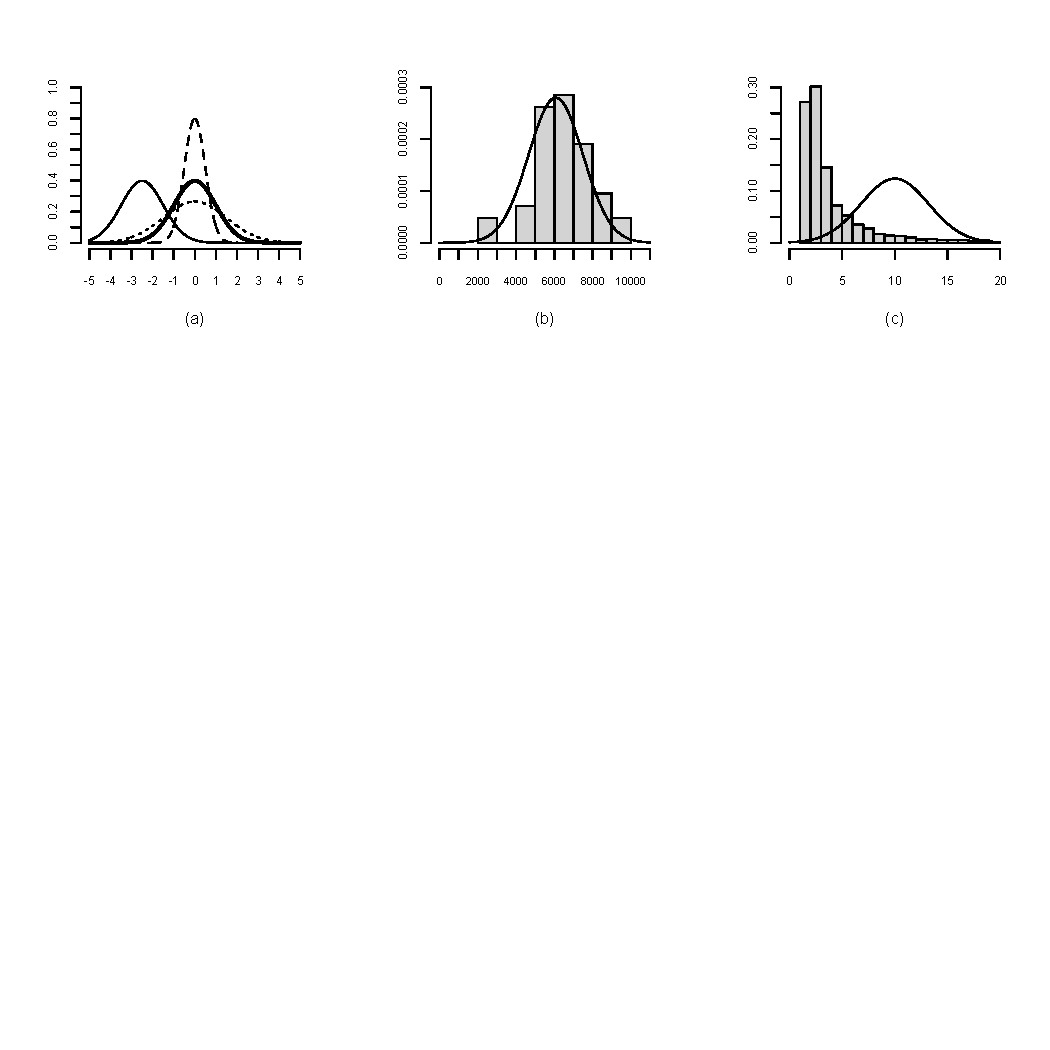
\includegraphics[width=\textwidth,keepaspectratio]{figures/normdist}
\end{figure}

You will often read that many natural phenomena approximate this distribution -- examples mentioned in textbooks are, invariably, the size and weight of organisms, frequently other characteristics of organisms such as skin area, blood pressure or IQ, and occasionally social phenomena like test scores and salaries. Figure \ref{fig:normdist}b show the distribution of body weight in a sample of swans collected for an environmental impact study \citep{fite_residues_1979}, and, indeed, it seems to follow, roughly, a normal distribution \is{distribution, normal} if we compare it to the bell curve superimposed on the figure.

Unfortunately, cardinal \is{cardinal data} measurements \is{measurement} derived from language data (such as the length \is{length} or of words, constituents, sentences, etc. or the distance \is{referential distance} to the last mention of a referent) are rarely (if ever) normally distributed \citep[see, e.g.,][51]{mcenery_corpus_2012}. Figure \ref{fig:normdist}c shows the distribution of the constituent length, \is{length} in number of words, of \textit{of}-phrases modifying nouns \is{noun} in the SUSANNE corpus (with \textit{of}-phrases with a length of more than 20 words removed as outliers). As you can see, they do not follow a normal distribution \is{distribution, normal} at all -- there are many more short \textit{of}-phrases than long ones, shifting the distribution further to the left and making it much narrower than it should be.

There are three broad ways of dealing with this issue. First, we could ignore it and hope that the \textit{t}-test \is{t-test} is robust enough to yield meaningful results despite this violation of the normality requirement. If this seems like a bad idea, this is because it is fundamentally a bad idea -- and statisticians warn against it categorically. \is{categorization} However, many social scientists regularly adopt this approach -- just like we did in the case study above. And in practice, this may be less of a problem than one might assume, since the \textit{t}-test \is{t-test} has been found to be fairly robust against violations of the normality requirement. However, we should not generally rely on this robustness, as linguistic data may depart from normality to quite an extreme degree. More generally, ignoring the prerequisites of a statistical procedure is not exactly good scientific practice -- the only reason I did it above was so you would not be too shocked when you see it done in actual research (which, inevitably, you will).

Second, and more recommendably, we could try to make the data fit the normality requirement. One way in which this is sometimes achieved in the many cases where data do not follow the normal distribution \is{distribution, normal} is to log\hyp{}transform the data (i.e., use the natural logarithm \is{logarithm} of the data instead of the data themselves). This often, but not always, causes the data to approximate a normal distribution more closely. However, this does not work in all cases (it would not, for example, bring the distribution in Figure \ref{fig:normdist}c much closer to a normal distribution, and anyway, transforming data carries its own set of problems.

Thus, third, and most recommendably, we could try to find a way around having to use a \textit{t}-test \is{t-test} in the first place. One way of avoiding a \textit{t}-test is to treat our non\hyp{}normally distributed \is{distribution, normal} cardinal \is{cardinal data} data as ordinal \is{ordinal data} data, as described in Chapter \ref{ch:quantifyingresearch}. We can then use the Mann\hyp{}Whitney \is{Mann-Whitney U test} U\hyp{}test, which does not require a normal distribution of the data. I leave it as an exercise to the reader to apply this test to the data in Table \ref{tab:posslengthwelch} (you know you have succeeded if your result for U is 137, $p < 0.01$).

Another way of avoiding the \textit{t}-test \is{t-test} is to find an operationalization \is{operationalization} of the phenomenon under investigation that yields rank data, \is{ordinal data} or, even better, nominal \is{nominal data} data in the first place. We could, for example, code \is{coding} the data in Table \ref{tab:posslengthwelch} in terms of a very simple nominal variable: \textvv{Longer Constituent} (with the variables \textvv{head} and \textvv{modifier}). For each case, we simply determine whether the head is longer than the modifier (in which case we assign the value head) or whether the modifier is longer than the head (in which case we assign the value \textvv{modifier}; we discard all cases where the two have the same length. \is{length} This gives us Table \ref{tab:posslengthnominal}.

\begin{table}[!htbp]
\caption{The influence of length on the choice between the two possessives}
\label{tab:posslengthnominal}
\begin{tabular}[t]{llccr}
\lsptoprule
 & & \multicolumn{2}{c}{\textvv{Possessive}} & \\
 & & \textvv{\textit{s}-possessive} & \textvv{\textit{of}-possessive} & Total \\
\midrule
\textvv{\makecell[lt]{Longer \\ Constituent}}
	& \textvv{head}
		& \makecell[t]{8\\(6.3)}
		& \makecell[t]{5\\(6.7)}
		& \makecell[t]{13\\} \\
	& \textvv{mod}
		& \makecell[t]{8\\(9.7)}
		& \makecell[t]{12\\(10.3)}
		& \makecell[t]{20\\} \\
\midrule
	& Total
		& \makecell[t]{16}
		& \makecell[t]{17}
		& \makecell[t]{33} \\
\lspbottomrule
\end{tabular}
\end{table}

The $\chi^2$ \is{chi-square test} value for this table is 0.7281, which at one degree of freedom means that the p value is larger than 0.05, so we would have to conclude that there is no influence of length \is{length} on the choice of possessive \is{possessive} construction. However, the deviations of the observed from the expected \is{frequency, expected} frequencies go in the right direction, so this may simply be due to the fact that our sample is too small (obviously, a serious corpus\hyp{}linguistic study would not be based on just 33 cases).

The normal\hyp{}distribution \is{distribution, normal} requirement is only one of several requirements that our data set must meet in order for particular statistical methods to be applicable. For example, many procedures for comparing group means -- including the more widely\hyp{}used \textit{Student} t\hyp{}test \is{t-test} -- can only be applied if the two groups have the same variance \is{variance} (roughly, if the measurements in both groups are spread out from the group means to the same extent), and there are tests to tell us this (for example, the \textit{F} test). Also, it makes a difference whether the two groups that we are comparing are independent of each other (as in the case studies presented here), or if they are dependent in that there is a correspondence between measures in the two groups. For example, if we wanted to compare the length of heads and modifiers in the \textit{s}-possessive, \is{possessive} we would have two groups that are dependent in that for any data point in one of the groups there is a corresponding data point in the other group that comes from the same corpus example. In this case, we would use a \textit{paired} test (for example, the matched\hyp{}pairs Wilcoxon \is{Mann-Whitney U test} test for ordinal \is{ordinal data} data and Student's paired t\hyp{}test \is{t-test} for cardinal \is{cardinal data} data).

\section{Complex research designs}
\label{sec:complexdesigns}

In Chapter \ref{ch:quantifyingresearch} and in this chapter so far, we have restricted our discussion to the simplest possible research designs \is{research design} -- cases where we are dealing with two variables with two values each. To conclude our discussion of statistical hypothesis testing, we will look at two cases of more complex designs -- one with two variables that each have more than two values, and one with more than two variables.

\subsection{Variables with more than two values}
\label{sec:morethantwovalues}

In our case studies involving the English possessive constructions, the dependent variable \textvv{(Type of) Possessive} was treated as binary -- we assumed that it had two values, \textvv{\textit{s}-possessive} and \textvv{\textit{of}-possessive}. \is{possessive} The dependent variables were more complex: the cardinal \is{cardinal data} variable \textvv{Length} \is{length} obviously has a potentially infinite number of values and the ordinal \is{ordinal data} variable \textvv{Animacy} \is{animacy} was treated as having ten values in our annotation \is{annotation} scheme. The nominal \is{nominal data} value \textvv{Discourse Status}, was treated like a binary variable (although potentially it has an infinite number of values, too).

Frequently, perhaps even typically, corpus linguistic research questions will be more complex, and we will be confronted with designs \is{research design} where both the dependent and the independent variable will have (or be treated as having) more than two values. Since we are most likely to deal with nominal \is{nominal data} variables in corpus linguistics, we will discuss in detail an example where both variables are nominal.

In the preceding chapters we treated as \textvv{\textit{s}-possessive} \is{possessive} constructions where the modifier is a possessive pronoun as well as constructions where the modifier is a proper name or a noun \is{noun} with a possessive clitic. \is{clitic} Given that the proportion of pronouns \is{pronoun} and nouns in general varies across language varieties \is{language variety} \citep{biber_longman_1999}, we might be interested to see whether the same is true for these three variants of the \textit{s}-possessive. Our dependent variable \textvv{Modifier of \textit{s}-Possessive} \is{possessive} would then have three values. The independent variable \textvv{Variety}, \is{language variety} being heavily dependent on the model of language varieties \is{language variety} we adopt -- or rather, on the nature of the text categories included in our corpus -- has an indefinite number of values. To keep things simple, let us distinguish just four broad text categories recognized in the British National Corpus (and many other corpora): \textvv{spoken}, \is{medium} \textvv{fiction}, \is{literary language} \textvv{newspaper} \is{newspaper language} and \textvv{academic}. This gives us a four\hyp{}by\hyp{}three design. \is{research design}

Searching the BNC Baby \is{BNC Baby} for words tagged \is{POS tagging} as possessive \is{possessive} pronouns \is{pronoun} and for words tagged unambiguously as proper names or common nouns \is{noun} yields the observed frequencies \is{frequency, observed} shown in the first line of each row in Table \ref{tab:texttypesposs}.

\begin{table}[!htbp]
\caption{Types of modifiers in the {\textit{s}}-possessive in different text categories}
\label{tab:texttypesposs}
\resizebox{\textwidth}{!}{%
\begin{tabular}[t]{lllS[table-format=5.2]S[table-format=5.2]S[table-format=5.2]S[table-format=5.2]}
\lsptoprule
 & & & \multicolumn{3}{c}{\textvv{Possessive Modifier}} & \\
 & & & \textvv{pronoun} & \textvv{proper name} & \textvv{noun} & \multicolumn{1}{l}{Total} \\
\midrule
\textvv{Variety} & \textvv{spoken} & \footnotesize{\textit{Obs.}} & 9593 & 768 & 604 & 10965 \\
& & \footnotesize{\textit{Exp.}} & 8378.38 & 1361.04 & 1225.58 & \\
& & \footnotesize{\textit{$\chi^2$\textit{-Comp.}}} & 176.08 & 258.40 & 315.25 & \\[2ex]
& \textvv{fiction} & \footnotesize{\textit{Obs.}} & 23755 & 2681 & 1998 & 28434 \\
& & \footnotesize{\textit{Exp.}} & \num{21726.49} & 3529.39 & 3178.12 & \\
& & \footnotesize{\textit{$\chi^2$\textit{-Comp.}}} & 189.39 & 203.94 & 438.21 & \\[2ex]
& \textvv{news} & \footnotesize{\textit{Obs.}} & 12857 & 4070 & 3585 & 20512 \\
& & \footnotesize{\textit{Exp.}} & \num{15673.27} & 2546.07 & 2292.66 & \\
& & \footnotesize{\textit{$\chi^2$\textit{-Comp.}}} & 506.04 & 912.14 & 728.47 & \\[2ex]
& \textvv{academic} & \footnotesize{\textit{Obs.}} & 8533 & 1373 & 1820 & 11726 \\
& & \footnotesize{\textit{Exp.}} & 8959.86 & 1455.50 & 1310.64 & \\
& & \footnotesize{\textit{$\chi^2$\textit{-Comp.}}} & 20.34 & 4.68 & 197.96 & \\
\midrule
& Total & & 54738 & 8892 & 8007 & 71637 \\
\lspbottomrule
\end{tabular}}
\end{table}

The expected \is{frequency, expected} frequencies and the $\chi^2$ \is{chi-square test} components are arrived at in the same way as for the two\hyp{}by\hyp{}two tables in the preceding chapter. First, for each cell, the sum of the column in which the cell is located is multiplied by the sum of the row in which it is located, and the result is divided by the table sum. For example, for the top left cell, we get the expected frequency

$$\frac{54738 \times 10965}{71637} = 8378.38,$$

the expected \is{frequency, expected} frequencies are shown in the second line of each cell. Next, for each cell, we calculate the $\chi^2$ \is{chi-square test} component. For example, for the top left cell, we get

$$\frac{(9593 - 8378.38)^2}{8378.38} = 176.08,$$

the corresponding values are shown in the third line of each cell. Adding up the individual $\chi^2$ \is{chi-square test} components gives us a $\chi^2$ value of 3950.89.

Using the formula given in \ref{ex:formuladf} above, Table \ref{tab:texttypesposs} has $(4 -1) \times (3 - 1) = 6$ degrees of freedom. As the $\chi^2$ \is{chi-square test} table in Section \ref{sec:chisquarecriticalvalues}, the required value for a significance \is{significance} level of 0.001 at 6 degrees of freedom is 22.46; the $\chi^2$ \is{chi-square test} value for Table \ref{tab:texttypesposs} is much higher than this, thus, our results are highly significant. We could summarize our findings as follows: ``The frequency \is{frequency} of pronouns, \is{pronoun} proper names and nouns \is{noun} as modifiers of the \textit{s}-possessive \is{possessive} differs highly significantly across text categories ($\chi^2 = 473.73, df = 12, p < 0.001$)''.

Recall that the mere fact of a significant \is{significance} association does not tell us anything about the strength of that association -- we need a measure of effect size. \is{effect size} In the preceding chapter, $\phi$ was introduced as an effect size for two\hyp{}by\hyp{}two tables (see (\ref{ex:formulaphi})). For larger tables, there is a generalized version of $\phi$, referred to as \textit{Cramer's V} (or, occasionally, as \textit{Cramer's $\phi$} or $\phi'$), which is calculated as follows (\textit{N} is the table sum, \textit{k} is the number of rows or columns, whichever is smaller):

\begin{exe}
\ex $\displaystyle{\text{Cramer's V} = \sqrt{\frac{\chi^2}{N \times (k - 1)}}}$
\label{ex:cramersv}
\end{exe}

For our table, this gives us

$$\sqrt{\frac{3950.89}{71637 \times (3-1)}} = 0.1661$$ % 0.166059607636466

Recall that the square of a correlation \is{correlation} coefficient tells us the proportion of the variance \is{variance} captured by our design, \is{research design} which, in this case, is 0.0275. In other words, \textvv{Variety} \is{language variety} explains less than three percent of the distribution \is{distribution, conditional} of \textit{s}-possessor modifier types across language varieties; \is{language variety} or ``This study has shown a very weak but highly significant \is{significance} influence of language variety on the realization of \textit{s}-possessor modifiers as pronouns, \is{pronoun} proper names or common nouns \is{noun} ($\chi^2 = 473.73, df = 12, p < 0.001, r = 0.0275$).'' \is{chi-square test}

Despite the weakness of the effect, this result confirms our expectation that general preferences for pronominal \is{pronoun} vs. nominal \is{noun} reference across language varieties \is{language variety} is also reflected in preferences for types of modifiers in the \textit{s}-possessive. \is{possessive} However, with the increased size of the contingency \is{contingency table} table, it becomes more difficult to determine exactly where the effect is coming from. More precisely, it is no longer obvious at a glance which of the intersections of our two variables contribute to the overall significance \is{significance} of the result in what way and to what extent.

To determine in what way a particular intersection contributes to the overall result, we need to compare the observed and expected \is{frequency, expected} frequencies in each cell. For example, there are 9593 cases of \textit{s}-possessives \is{possessive} with pronominal modifiers in spoken \is{medium} language, where 8378.38 are expected, showing that pronominal \is{pronoun} modifiers are more frequent in spoken language than expected by chance. \is{chance} In contrast, there are 8533 such modifiers in academic \is{academic language} language, where 8959.86 are expected, showing that they are less frequent in academic language than expecte by chance. This comparison is no different from that which we make for two\hyp{}by\hyp{}two tables, but with increasing degrees of freedom, the pattern becomes less predictable. It would be useful to visualize the relation between observed and expected \is{frequency, expected} frequencies for the entire table in a way that would allow us to take them in at a glance.

To determine to what extent a particular intersection contributes to the overall result, we need to look at the size of the $\chi^2$ components -- the larger the component, the greater its contribution to the overall $\chi^2$ \is{chi-square test} value. In fact, we can do more than simply compare the $\chi^2$ components to each other -- we can determine for each component, whether it, in itself, is statistically significant. \is{significance} In order to do so, we first imagine that the large contingency \is{contingency table} table (in our case, the 4\hyp{}by\hyp{}3 table) consists of a series of tables with a single cell each, each containing the result for a single intersection of our variables.

We now treat the $\chi^2$ component as a $\chi^2$ value in its own right, checking it for statistical significance \is{significance} in the same way as the overall $\chi^2$ value. In order to do so, we first need to determine the degrees of freedom for our one\hyp{}cell tables -- obviously, this can only be 1. Checking the table of critical $\chi^2$ \is{chi-square test} values in Section \ref{sec:chisquarecriticalvalues}, we find, for example, that the $\chi^2$ component for the intersection \textvv{pronoun} \is{pronoun} $\cap$ \textvv{spoken}, \is{medium} which is 176.08, is higher than the critical value 10.83, suggesting that this intersection's contribution is significant \is{significance} at p < 0.001.

However, matters are slightly more complex: by looking at each intersection separately, we are essentially treating each cell as an independent result -- in our case, it is as if we had performed twelve tests instead of just one. Now, recall that levels of significance \is{significance} are based on probabilities \is{probability of error} of error -- for example, $p = 0.05$ means, roughly, that there is a five percent likelihood that a result is due to chance. \is{chance} Obviously, the more tests we perform, the more likely it becomes that one of the results will, indeed, be due to chance \is{chance} -- for example, if we had performed twenty tests, we would expect one of them to yield a significant result at the 5\hyp{}percent level, because $20 \times 0.05 = 1.00$.

To avoid this situation, we have to correct the levels of significance when performing multiple tests on the same set of data. The simplest way of doing so is the so\hyp{}called Bonferroni \is{Bonferroni correction} correction, which consists in dividing the conventionally agreed\hyp{}upon significance levels by the number of tests we are performing. In the case of Table \ref{tab:texttypesposs}, this means dividing them by twelve, giving us significance \is{significance} levels of $\nicefrac{0.05}{12} = 0.004167$ (significant), $\nicefrac{0.01}{12} = 0.000833$ (very significant), and $\nicefrac{0.001}{12} = 0.000083$ (highly significant).\footnote{It should be noted that the Bonferroni \is{Bonferroni correction} correction is extremely conservative, but it has the advantage of being very simple to apply (see \citealt{shaffer_multiple_1995} for an overview corrections for multiple testing, including many that are less conservative than the Bonferroni correction).} Our table does not give the critical $\chi^2$-values \is{chi-square test} for these levels, but the value for the the intersection \textvv{pronoun} \is{pronoun} $\cap$ \textvv{spoken}, \is{medium} 176.08, is larger than the value required for the next smaller level (0.00001, with a critical value of 24.28), so we can be certain that the contribution of this intersection is, indeed, highly significant. \is{significance} Again, it would be useful to summarize the degrees of significance in such a way that they can be assessed at a glance.

There is no standard way of representing the way in, and degree to, which each cell of a complex table contributes to the overall result, but the representation in Table \ref{tab:texttypesposscont} seems reasonable: in each cell, the first line contains either a plus (for ``more frequent than expected'') \is{frequency, expected} or a minus (for ``less frequent than expected''); the second line contains the $\chi^2$-component, \is{chi-square test} and the third line contains the (corrected) level of significance \is{significance} (using the standard convention of representing them by asterisks -- one for each level of significance).

\begin{table}[!htbp]
\caption{Types of modifiers in the \textit{s}-possessive in different text categories: Contributions of the individual intersections}
\label{tab:texttypesposscont}
\begin{tabular}[t]{llccc}
\lsptoprule
 & & \multicolumn{3}{c}{\textvv{Possessive Modifier}} \\
 & & \textvv{pronoun} & \textvv{proper name} & \textvv{noun} \\
\midrule
\textvv{Variety} & \textvv{spoken} & $+$ & $-$ & $-$ \\
& & 176.08 & 258.40 & 315.25 \\
& & ***** & ***** & ***** \\[2ex]
& \textvv{fiction} & $+$ & $-$ & $-$ \\
& & 189.39 & 203.94 & 438.21 \\
& & ***** & ***** & ***** \\[2ex]
& \textvv{news} & $-$ & $+$ & $+$ \\
& & 506.04 & 912.14 & 728.47 \\
& & ***** & ***** & ***** \\[2ex]
& \textvv{academic} & $-$ & $-$ & $+$ \\
& & 20.34 & 4.68 & 197.96 \\
& & **** & n.s. & ***** \\
\lspbottomrule
\end{tabular}
\end{table}
% me: levels of significance
% me: 8.209716 11.165482 15.481123 19.859825 24.279218

This table presents the complex results at a single glance; they can now be interpreted. Some patterns now become obvious: For example, spoken \is{medium} language and fiction \is{literary language} are most similar to each other -- they both favor pronominal \is{pronoun} modifiers, while proper names and common nouns \is{noun} are disfavored, and the $\chi^2$-components \is{chi-square test} for these preferences are very similar. Also, if we posit a kind of gradient of referent familiarity from pronouns over proper names to nouns, we can place spoken \is{medium} language and fiction at one end, academic \is{academic language} language at the other, and newspaper \is{newspaper language} language somewhere in the middle.

\subsection{Designs with more than two variables}

Note that from a certain perspective the design \is{research design} in Table \ref{tab:texttypesposscont} is flawed: the variable \textvv{Variety} \is{language variety} actually conflates at least two variables that are theoretically independent: \textvv{Medium} \is{medium} (with the variables \textvv{spoken} and \textvv{written}, and \textvv{Discourse Domain} (in our design with the variables \textvv{news (recounting of actual events)}, \is{newspaper language} \textvv{fiction (recounting of imaginary events)} \is{literary language} and \textvv{academic (recounting of scientific ideas, procedures and results)}. These two variables are independent in that there is both written and spoken language to be found in each of these discourse domains. They are conflated in our variable \textvv{Variety} \is{language variety} in that one of the four values is spoken and the other three are written language, and in that the text category \textvv{spoken} is not differentiated by topic. There may be reasons to ignore this conflation \textit{a priori}, as we have done -- for example, our model may explicitly assume that differentiation by topic happens only in the written domain. But even then, it would be useful to treat \textvv{Medium} \is{medium} and \textvv{Discourse Domain} as independent variables, just in case our model is wrong in assuming this.

In contrast to all examples of research designs \is{research design} we have discussed so far, which involved just two variables and were thus \textit{bivariate}, \is{bivariate analysis} this design would be \textit{multivariate}: \is{multivariate analysis} there is more than one independent variable whose influcence on the dependent variable we wish to assess. Such multivariate research designs are often useful (or even necessary) even in cases where the variables in our design are not conflations of more basic variables.

In the study of language use, we will often -- perhaps even typically -- be confronted with a fragment of reality that is too complex to model in terms of just two variables.

In some cases, this may be obvious from the outset: we may suspect from previous research that a particular linguistic phenomenon depends on a range of factors, as in the case of the choice between the \textit{s}- and the \textit{of}-possessive, \is{possessive} which we saw in the preceding chapters had long been hypothesized to be influenced by the animacy, \is{animacy} the length \is{length} and\slash or the givenness \is{givenness} of the modifier.

In other cases, the multivariate \is{multivariate analysis} nature of the phenomenon under investigation may emerge in the course of pursuing an initially bivariate \is{bivariate analysis} design. \is{research design} For example, we may find that the independent variable under investigation has a statistically significant \is{significance} influence on our dependent variable, but that the effect size \is{effect size} is very small, suggesting that the distribution \is{distribution, conditional} of the phenomenon in our sample is conditioned by more than one influencing factor.

Even if we are pursuing a well\hyp{}motivated bivariate \is{bivariate analysis} research design \is{research design} and find a significant \is{significance} influence with a strong effect size, \is{effect size} it may be useful to take additional potential influencing factors into account: since corpus data are typically unbalanced, there may be hidden correlations \is{correlation} between the variable under investigation and other variables, that distort the distribution \is{distribution, conditional} of the phenomenon in a way that suggests a significant influence where no such influence actually exists.

The next subsection will use the latter case to demonstrate the potential shortcomings of bivariate \is{bivariate analysis} designs \is{research design} and the subsection following it will present a solution. Note that this solution is considerably more complex than the statistical procedures we have looked at so far and while it will be presented in sufficient detail to enable the reader in principle to apply it themselves, some additional reading will be highly advisable.

\subsubsection{A danger of bivariate designs}

In recent years, attention has turned to sociolinguistic \is{sociolinguistics} factors potentially influencing the choice between the {s}-possessive \is{possessive} and the {of}-construction. It has long been known that the level of formality has an influence (\citealt{jucker_genitive_1993}, also \citealt{grafmiller_variation_2014}), but recently, more traditional sociolinguistic \is{sociolinguistics} variables like \textvv{Sex} and \textvv{Age} have been investigated. The results suggest that the latter has an influence, while the former does not -- for example, \citet{jankowski_genitives_2014} find no influence of sex, but find that age \is{age} has an influence under some conditions, with young speakers using the \textit{s}-genitive more frequently than old speakers for organizations and places; \citet{vogel_rhythms_2015} find a similar, more general influence of age. \is{age}

Let us take a look at the influence of \textvv{Sex} and \textvv{Age} on the choice between the two possessives \is{possessive} in the spoken \is{medium} part of the BNC. \is{BNC} Since it is known that women tend to use pronouns \is{pronoun} more than men do (see Case Study \ref{sec:adeductiveapproachtosexdifferences} in Chapter \ref{ch:text}), let us exclude possessive pronouns and operationalize \is{operationalization} the \textvv{\textit{s}-possessive} as ``all tokens tagged \is{POS tagging} \texttt{POS} in the BNC'', \is{BNC} which will capture the possessive clitic \is{clitic} \textit{'s} and zero possessives (on common nouns \is{noun} ending in alveolar fricatives). Since the spoken \is{medium} part of the BNC is too large to identify \textit{of}-possessives manually, \is{manual analysis} let us operationalize \is{operationalization} them somewhat crudely as ``all uses of the preposition \is{adposition} \textit{of}''; this encompasses not just \textit{of}-possessives, \is{possessive} but also the quantifying and partitive \textit{of}-constructions that we manually \is{manual analysis} excluded in the preceding chapters, the complementation of adjectives \is{adjective} like \textit{aware} and \textit{afraid}, verbs \is{verb} like \textit{consist} and \textit{dispose}, etc. On the one hand, this makes our case study less precise, on the other hand, any preference for \textit{of}-constructions may just be a reflex of a general preference for the preposition \is{adposition} \textit{of}, in which case we would be excluding relevant data by focusing on \textit{of}-constructions. Anyway, our main point will be one concerning statistical methodology, so it does not matter too much either way.

So, let us query all tokens tagged \is{POS tagging} as possessives \is{possessive} (POS) or the preposition \is{adposition} of (PRF) in the spoken \is{medium} part of the BNC, \is{BNC} discarding all hits for which the information about speaker sex or speaker age \is{age} is missing. Let us further exclude the age \is{age} range 0-14, as it may include children who have not fully acquired \is{language acquisition} the grammar of the language, and the age \is{age} range 60+ as too unspecific. To keep the design \is{research design} simple, let us recode all age \is{age} classes between 15 and 44 years of age \is{age} as \textvv{young} and the age \is{age} range 45-59 als \textvv{old} (I fall into the latter, just in case someone thinks this category label discriminates people in their prime). Let us further accept the categorization \is{categorization} of speakers into \textit{male} and \textit{female} that the makers of the BNC \is{BNC} provide.

Table \ref{tab:posssexindiv} shows the intersections of \textvv{Construction} and \textvv{Sex} in the results of this query.

\begin{table}[!htbp]
\caption{The influence of \textvv{Sex} on the choice between the two possessives}
\label{tab:posssexindiv}
\begin{tabular}[t]{llccr}
\lsptoprule
 & & \multicolumn{2}{c}{\textvv{Construction}} & \\
 & & \textvv{pos} & \textvv{of} & Total \\
\midrule
\textvv{\makecell[lt]{Sex}}
	& \textvv{female}
		& \makecell[t]{\num{3483}\\\small{(\num{2432.89})}}
		& \makecell[t]{\num{20419}\\\small{(\num{21469.11})}}
		& \makecell[t]{\num{23902}} \\
	& \textvv{male}
		& \makecell[t]{\num{3515}\\\small{(\num{4565.11})}}
		& \makecell[t]{\num{41335}\\\small{(\num{40284.89})}}
		& \makecell[t]{\num{44850}} \\
\midrule
	& Total
		& \makecell[t]{\num{6998}}
		& \makecell[t]{\num{61754}}
		& \makecell[t]{\num{68752}} \\
\lspbottomrule
\end{tabular}
\end{table}
% me: chisq.test(matrix(c(3483,3515,20419,41335),ncol=2),corr=FALSE)

Unlike the studies mentioned above, we find a clear influence of \textvv{Sex} on \textvv{Construction}, with female speakers preferring the \textit{s}-possessive \is{possessive} and male speakers preferring the \textit{of}-construction(s). The difference is highly significant, \is{significance} although the effect size \is{effect size} is rather weak ($\chi^2$ = 773.55, df = 1, p < 0.001, $\phi$ = 0.1061). \is{chi-square test}

Next, let us look at the intersections of \textvv{Construction} and \textvv{Sex} in the results of our query, which are shown in Table \ref{tab:possageindiv}.

\begin{table}[!htbp]
\caption{The influence of \textvv{Age} on the choice between the two possessives}
\label{tab:possageindiv}
\begin{tabular}[t]{llccr}
\lsptoprule
 & & \multicolumn{2}{c}{\textvv{Construction}} & \\
 & & \textvv{pos} & \textvv{of} & Total \\
\midrule
\textvv{\makecell[lt]{Age}}
	& \textvv{old}
		& \makecell[t]{\num{2450}\\\small{(\num{2746.70})}}
		& \makecell[t]{\num{24535}\\\small{(\num{24238.30})}}
		& \makecell[t]{\num{26985}} \\
	& \textvv{young}
		& \makecell[t]{\num{4548}\\\small{(\num{4251.30})}}
		& \makecell[t]{\num{37219}\\\small{(\num{37515.70})}}
		& \makecell[t]{\num{41767}} \\
\midrule
	& Total
		& \makecell[t]{\num{6998}}
		& \makecell[t]{\num{61754}}
		& \makecell[t]{\num{68752}} \\
\lspbottomrule
\end{tabular}
\end{table}
% me: chisq.test(matrix(c(2450,4548,24535,37219),ncol=2),corr=FALSE)

Like previous studies, we find a significant \is{significance} effect of age, \is{age} with younger speakers preferring the \textit{s}-possessive \is{possessive} and older speakers preferring the \textit{of}-construction(s). Again, the difference is highly significant, but the effect is extremely weak ($\chi^2$ = 58.73, df = 1, p < 0.001, $\phi$ = 0.02922).

We might now be satisfied that both speaker age \is{age} and speaker sex have an influence on the choice between the two constructions. However, there is a potential problem that we need to take into account: the values of the variables \textvv{Sex} and \textvv{Age} and their intersections are not necessarily distributed \is{distribution, conditional} evenly in the subpart of the BNC \is{BNC} used here; although the makers of the corpus were careful to include a broad range of speakers of all ages, sexes (and class memberships, ignored in our study), they did not attempt to balance all these demographic \is{demography} variables, let alone their intersections. So let us look at the intersection of \textvv{Sex} and \textvv{Age} in the results of our query. These are shown in Table \ref{tab:sexagebnc}.

\begin{table}[!htbp]
\caption{\textvv{Sex} and \textvv{Age} in the BNC}
\label{tab:sexagebnc}
\begin{tabular}[t]{llccr}
\lsptoprule
 & & \multicolumn{2}{c}{\textvv{Age}} & \\
 & & \textvv{old} & \textvv{young} & Total \\
\midrule
\textvv{\makecell[lt]{Sex}}
	& \textvv{female}
		& \makecell[t]{\num{6559}\\\small{(\num{9381.48})}}
		& \makecell[t]{\num{17343}\\\small{(\num{14520.52})}}
		& \makecell[t]{\num{23902}} \\
	& \textvv{male}
		& \makecell[t]{\num{20426}\\\small{(\num{17603.52})}}
		& \makecell[t]{\num{24424}\\\small{(\num{27246.48})}}
		& \makecell[t]{\num{44850}} \\
\midrule
	& Total
		& \makecell[t]{\num{26985}}
		& \makecell[t]{\num{41767}}
		& \makecell[t]{\num{68752}} \\
\lspbottomrule
\end{tabular}
\end{table}
% me: chisq.test(matrix(c(6559,20426,17343,24424),ncol=2),corr=FALSE)
% me: X-squared = 2142.7, df = 1, p-value < 2.2e-16

There are significantly \is{significance} fewer hits produced by old women and significantly more produced by young women in our sample, and, conversely, significantly fewer hits produced by young men and significantly more produced by old men. This overrepresentation of young women and old men is not limited to our sample, but characterizes the spoken \is{medium} part of the BNC \is{BNC} in general, which should intrigue feminists and psychoanalysts; for us, it suffices to know that the asymmetries in our sample are highly significant, \is{significance} with an effect size \is{effect size} larger than that of that in the preceding two tables ($\chi^2$ = 2142.72, df = 1, p < 0.001, $\phi$ = 0.1765). \is{chi-square test}

This correlation \is{correlation} in the corpus of \textvv{old} and \textvv{male} on the one hand and \textvv{young} and \textvv{female} on the other may well be enough to distort the results such that a linguistic behavior typical for female speakers may be wrongly attributed to young speakers (or vice versa), and, correspondingly, a linguistic behavior typical for male speakers may be wrongly interpreted to old speakers (or vice versa). More generally, the danger of bivariate \is{bivariate analysis} designs \is{research design} is that a variable we have chosen for investigation is correlated \is{correlation} with one or more variables ignored in our research design, whose influence thus remains hidden. A very general precaution against this possibility is to make sure that the corpus (or our sample) is balanced with respect to all potentially confounding variables. In reality, this is difficult to achieve and may in fact be undesirable, since we might, for example, want our corpus (or sample) to reflect the real\hyp{}world correlation \is{correlation} of speaker variables).

Therefore, we need a way of including multiple independent variables in our research designs \is{research design} even if we are just interested in a single independent variable, but all the more so if we are interested in the influence of several independent variables. It may be the case, for example, that both \textvv{Sex} and \textvv{Age} influence the choice between \textit{'s} and \textit{of}, either in that the two effects add up, or in that they interact in more complex ways.

\subsubsection{Configural frequency analysis}

There is a range of multivariate \is{multivariate analysis} statistical methods that are routinely used in corpus linguistics, such as the ANOVA mentioned at the end of the previous chapter for situations where the dependent variable is measured \is{measurement} in terms of cardinal \is{cardinal data} numbers, and various versions of logistic regression for situations where the dependent variable is ordinal \is{ordinal data} or nominal. \is{nominal data}

In this book, I will introduce multivariate \is{multivariate analysis} designs \is{research design} using \textit{Configural Frequency Analysis} (CFA), \is{configural frequency analysis} a straightforward extension of the $\chi^2$ \is{chi-square test} test to designs with more than two nominal \is{nominal data} variables. This method has been used in psychology \is{psychology} and psychiatry since the 1970s, and while it has never become very wide\hyp{}spread, it has, in my opinion, a number of didactic advantages over other methods, when it comes to understanding multivariate \is{multivariate analysis} research designs. \is{research design} Most importantly, it is conceptually very simple (if you understand the $\chi^2$ \is{chi-square test} test, you should be able to understand CFA), and the results are very transparent (they are presented as observed and expected \is{frequency, expected} frequencies of intersections of variables.

This does not mean that CFA \is{configural frequency analysis} is useful \textit{only} as a didactic tool -- it has been applied fruitfully to linguistic research issues, for example, in the study of language disorders \citep{lautsch_strategische_1988}, educational linguistics \citep{fujioka_views_1997}, psycholinguistics \is{psycholinguistics} \citep{hsu_infant_2000} and social psychology \is{psychology} \citep{christmann_components_2000}. An early suggestion to apply it to corpus data is found in \citet{schmilz_zahlen_1983}, but the first actual such applications that I am aware of are \citet{gries_evidence_2002, gries_characteristics_2004}. Since Gries introduced the method to corpus linguistics, it has become a minor but nevertheless well\hyp{}established corpus\hyp{}linguistic research tool for a range of linguistic phenomena (see, e.g., \citealt{stefanowitsch_covarying_2005}, \citealt{kristiansen_channel_2008}, \citealt{liu_is_2010}, \citealt{goschler_beyond_2013}, \citealt{buschfeld_cognitive_2014}, \citealt{hilpert_constructional_2015} and others).

% me: LIT add examples

As hinted at above, in its simplest variant, configural \is{configural frequency analysis} frequency analysis is simply a $\chi^2$ \is{chi-square test} test on a contingency \is{contingency table} table with more than two dimensions. There is no logical limit to the number of dimensions, but if we insist on calculating this statistic manually (rather than, more realistically, letting a specialized software package do it for us), then a three\hyp{}dimensional table is already quite complex to deal with. Thus, we will not go beyond three dimensions here or in the case studies in the second part of this book.

A three\hyp{}dimensional contingency \is{contingency table} table would have the form of a cube, as shown in Figure \ref{fig:cfaschematic}. The smaller cube represents the cells on the far side of the big cube seen from the same perspective and the smallest cube represents the cell in the middle of the whole cube). As before, cells are labeled by subscripts: the first subscript stands for the values and totals of the dependent variable, the second for those of the first independent variable, and the third for those of the second independent variable.

\begin{figure}[!htbp]
\caption{A three\hyp{}dimensional contingency table}
\label{fig:cfaschematic}
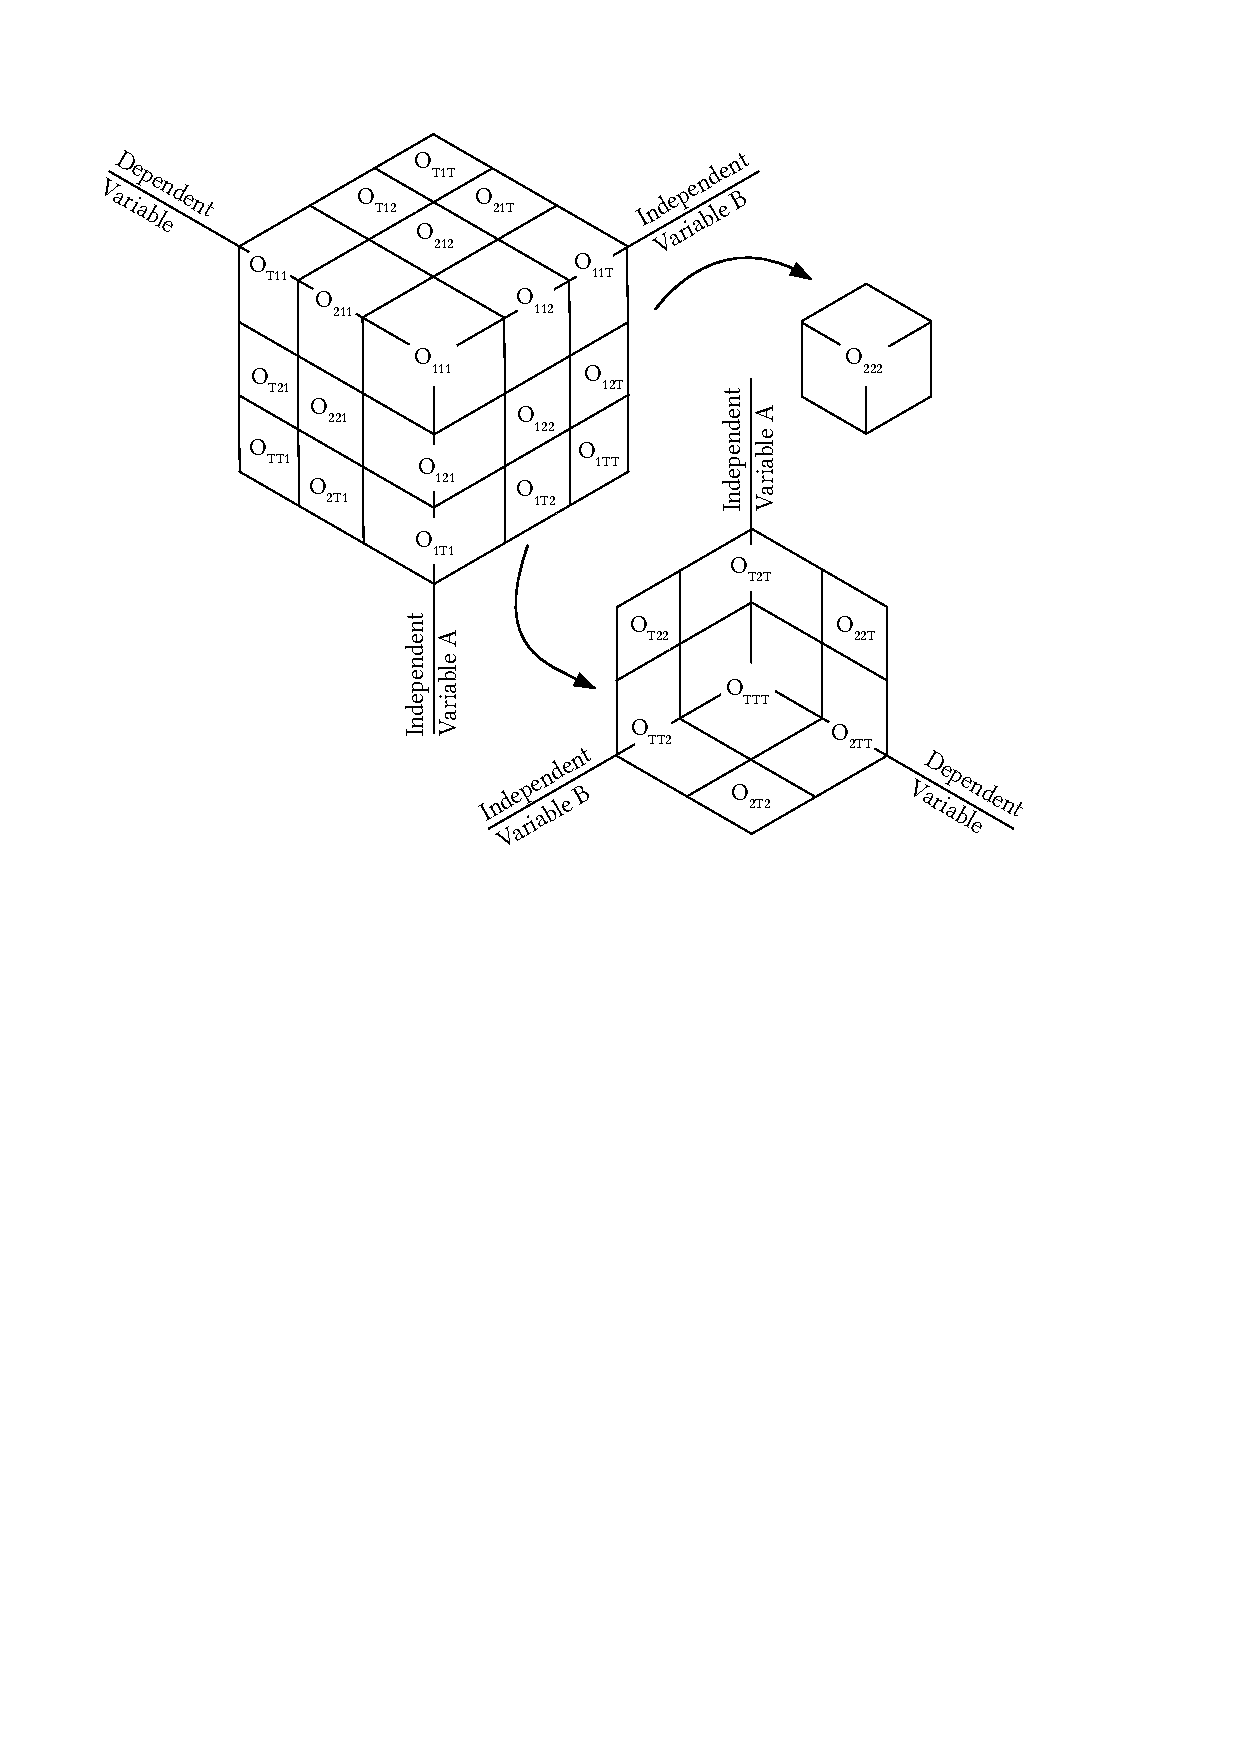
\includegraphics[width=\textwidth,keepaspectratio]{figures/cfaschematic}
\end{figure}

While this kind of visualization is quite useful in grasping the notion of a three\hyp{}dimensional contingency \is{contingency table} table, it would be awkward to use it as a basis for recording observed frequencies \is{frequency, observed} or calculating the expected \is{frequency, expected} frequencies. Thus, a possible two\hyp{}dimensional representation is shown in Table \ref{tab:cfaschematictable}. \is{configural frequency analysis} In this table, the first independent variable is shown in the rows, and the second independent variable is shown in the three blocks of three columns (these may be thought of as three ``slices'' of the cube in Figure \ref{fig:cfaschematic}), and the dependent variable is shown in the columns themselves.

\begin{table}[!htbp]
\caption{A two\hyp{}dimensional representation of a three\hyp{}dimensional contingency table}
\label{tab:cfaschematictable}
\resizebox{\textwidth}{!}{
\begin{tabular}[t]{lccc|ccc|ccc}
\lsptoprule
 &
 	\multicolumn{3}{c}{\textvv{iv\textsubscript{B} 1}} &
 	\multicolumn{3}{c}{\textvv{iv\textsubscript{B} 2}} &
 	\multicolumn{3}{c}{\textvv{iv\textsubscript{B}} Total} \\
\midrule
 &
 	\textvv{dv 1} &
 	\textvv{dv 2} &
 	\textvv{dv} Total &
 	
 	\textvv{dv 1} &
 	\textvv{dv 2} &
 	\textvv{dv} Total &
 	
 	\textvv{dv 1} &
 	\textvv{dv 2} &
 	\textvv{dv} Total \\
\midrule
\textvv{iv\textsubscript{A}} 1 &

	O\textsubscript{111} &
	O\textsubscript{112} &
	O\textsubscript{11T} &

	O\textsubscript{121} &
	O\textsubscript{122} &
	O\textsubscript{12T} &

	O\textsubscript{1T1} &
	O\textsubscript{1T2} &
	O\textsubscript{1TT} \\
	
\textvv{iv\textsubscript{A}} 2 &

	O\textsubscript{211} &
	O\textsubscript{212} &
	O\textsubscript{21T} &
	
	O\textsubscript{221} &
	O\textsubscript{222} &
	O\textsubscript{22T} &
	
	O\textsubscript{2T1} &
	O\textsubscript{2T2} &
	O\textsubscript{2TT} \\

\midrule

\textvv{iv\textsubscript{A}} Total &

	O\textsubscript{T11} &
	O\textsubscript{T12} &
	O\textsubscript{T1T} &
	
	O\textsubscript{T21} &
	O\textsubscript{T22} &
	O\textsubscript{T2T} &
	
	O\textsubscript{TT1} &
	O\textsubscript{TT2} &
	O\textsubscript{TTT} \\

\lspbottomrule
\end{tabular}}
\end{table}


Given this representation, the expected \is{frequency, expected} frequencies for each intersection of the three variables can now be calculated in a way that is similar (but not identical) to that used for two\hyp{}dimensional tables. Table \ref{tab:cfaschematicformula} shows the formulas for each cell as well as those marginal sums needed for the calculation.

\begin{table}[!htbp]
\caption{Calculating expected frequencies in a three\hyp{}dimensional contingency table}
\label{tab:cfaschematicformula}
\resizebox{\textwidth}{!}{
\begin{tabular}[t]{lccccccccc}
\lsptoprule
 &
 	\multicolumn{3}{c}{\textvv{iv\textsubscript{B} 1}} &
 	\multicolumn{3}{c}{\textvv{iv\textsubscript{B} 2}} &
 	\multicolumn{3}{c}{\textvv{iv\textsubscript{B}} Total} \\
\lsptoprule
 &
 	\textvv{dv 1} &
 	\textvv{dv 2} &
 	\textvv{dv} Total &
 	
 	\textvv{dv 1} &
 	\textvv{dv 2} &
 	\textvv{dv} Total &
 	
 	\textvv{dv 1} &
 	\textvv{dv 2} &
 	\textvv{dv} Total \\
\midrule
\textvv{iv\textsubscript{A}} 1 &

	${O_{T1T} \times O_{1TT} \times O_{TT1}} \over {O_{TTT}}^2$ &
	${O_{T1T} \times O_{1TT} \times O_{TT2}} \over {O_{TTT}}^2$ &
	 &

	${O_{T1T} \times O_{2TT} \times O_{TT1}} \over {O_{TTT}}^2$ &
	${O_{T1T} \times O_{2TT} \times O_{TT2}} \over {O_{TTT}}^2$ &
	 &

	 &
	 &
	 \\[2ex]
	
\textvv{iv\textsubscript{A}} 2 &

	${O_{T2T} \times O_{1TT} \times O_{TT1}} \over {O_{TTT}}^2$ &
	${O_{T2T} \times O_{1TT} \times O_{TT2}} \over {O_{TTT}}^2$ &
	 &
	
	${O_{T2T} \times O_{2TT} \times O_{TT1}} \over {O_{TTT}}^2$ &
	${O_{T2T} \times O_{2TT} \times O_{TT2}} \over {O_{TTT}}^2$ &
	 &
	
	 &
	 &
	 \\[2ex]

\textvv{iv\textsubscript{A}} Total &

	 &
	 &
	 &
	
	 &
	 &
	 &
	
	 &
	 &
	 \\

\lspbottomrule
\end{tabular}}
\end{table}

Once we have calculated the expected \is{frequency, expected} frequencies, we proceed exactly as before: we derive each cell's $\chi^2$ \is{chi-square test} component by the standard formula $\nicefrac{(O - E)^2}{E}$ and then add up these components to give us an overall $\chi^2$ value for the table, which can then be checked for significance. \is{significance} The degrees of freedom of a three\hyp{}dimensional contingency \is{contingency table} table are calculated by the following formula (where k is the number of values of each variable and the subscripts refer to the variables themselves):

\begin{exe}
\ex
$df = (k_1 \times k_2 \times k_3) - (k_1 + k_2 + k_3) + 2$
\label{ex:degreesoffreedom3D}
\end{exe}

In our case, each variable has two values, thus we get $(2 \times 2 \times 2) - (2 + 2 + 2) + 2 = 4$. More interestingly, we can also look at the individual cells to determine whether their contribution to the overall value is significant). \is{significance} In this case, as before, each cell has one degree of freedom and the significance levels have to be adjusted for multiple testing. In CFA, \is{configural frequency analysis} an intersection of variables whose observed frequency \is{frequency, observed} is significantly higher than expected \is{frequency, expected} is referred to as a \textit{type} \is{type (CFA)} and one whose observed frequency is significantly lower is referred to as an \textit{antitype} \is{antitype (CFA)} (but if we do not like this terminology, we do not have to use it and can keep talking about ``more or less frequent than expected, \is{frequency, expected} as we do with bivariate \is{bivariate analysis} $\chi^2$ \is{chi-square test} tests).

Let us apply this method to the question described in the previous sub\hyp{}section. Table \ref{tab:possexagemulti} shows the observed and expected \is{frequency, expected} frequencies of the two possessive \is{possessive} constructions by \textvv{Speaker Age} and \textvv{Speaker Sex}, as well as the corresponding $\chi^2$ \is{chi-square test} components.\footnote{Note one important fact about multi\hyp{}dimensional contingency \is{contingency table} tables that may be confusing: if we add up the expected \is{frequency, expected} frequencies of a given column, their sum will not usually correspond to the sum of the observed frequencies \is{frequency, observed} in that column (in contrast to two\hyp{}dimensional tables, where this is necessarily the case). Instead, the sum of the observed and expected frequencies in each \textit{slice} is identical.} For expository purposes, the table also shows for each cell the significance \is{significance} level of these components (which is ``highly significant'' for almost all of them), and the direction of deviation from the expected \is{frequency, expected} frequencies (i.e., whether the intersection is a ``type'', \is{type (CFA)} marked \is{annotation} by a plus sign, or an ``antitype'', \is{antitype (CFA)} marked by a minus sign).

\begin{table}[!htbp]
\caption{Sex, Age and Possessives Multivariate (BNC Spoken)}
\label{tab:possexagemulti}
\resizebox{\textwidth}{!}{%
\begin{tabular}[t]{l|ccc|ccc|r}
\lsptoprule
& \multicolumn{3}{c|}{\textvv{female}} & \multicolumn{3}{c|}{\textvv{male}} & \\
\textvv{Constr.} & \textvv{young} & \textvv{old} & \makecell[b]{Total \\ \textvv{female}} & \textvv{young} & \textvv{old} & \makecell[b]{Total \\ \textvv{male}} & Total \\
\midrule
\textvv{\makecell[tl]{\textvv{pos}}}
% me: female-young
	& \makecell[t]{\begin{tabular}[t]{lS[table-format=4.2]}
		\small{\textit{Obs.:}} & 2548 \\
		\small{\textit{Exp.:}} & 1477.9876 \\
		\small{\textit{$\chi^2$:}} & 774.6523328 \\
		\small{\textit{p:}} & \multicolumn{1}{c}{***} \\
		\small{\textit{Type:}} & \multicolumn{1}{c}{$+$} \\
		\end{tabular}}
% me: female-old
	& \makecell[t]{\begin{tabular}[t]{lS[table-format=4.2]}
		\small{\textit{Obs.:}} & 935 \\
		\small{\textit{Exp.:}} & 954.9045 \\
		\small{\textit{$\chi^2$:}} & 0.4148983 \\
		\small{\textit{p:}} & \multicolumn{1}{c}{n.s.} \\
		\small{\textit{Type:}} & \multicolumn{1}{c}{--} \\
		\end{tabular}}
% me: female-total
	& \makecell[t]{3483}
% me: male-young
	& \makecell[t]{\begin{tabular}[t]{lS[table-format=4.2]}
		\small{\textit{Obs.:}} & 2000 \\
		\small{\textit{Exp.:}} & 2773.3137 \\
		\small{\textit{$\chi^2$:}} & 215.6315971 \\
		\small{\textit{p:}} & \multicolumn{1}{c}{***} \\
		\small{\textit{Type:}} & \multicolumn{1}{c}{--} \\
		\end{tabular}}
% me: male-old
	& \makecell[t]{\begin{tabular}[t]{lS[table-format=4.2]}
		\small{\textit{Obs.:}} & 1515 \\
		\small{\textit{Exp.:}} & 1791.7942 \\
		\small{\textit{$\chi^2$:}} & 42.7588434 \\
		\small{\textit{p:}} & \multicolumn{1}{c}{***} \\
		\small{\textit{Type:}} & \multicolumn{1}{c}{--} \\
		\end{tabular}}
% me: male-total
	& \makecell[t]{3515}
% me: total
	& \makecell[t]{6998} \\[2.2cm]
\textvv{\makecell[tl]{\textvv{of}}}
% me: female-young
	& \makecell[t]{\begin{tabular}[t]{lS[table-format=4.2]}
		\small{\textit{Obs.:}} & 14795 \\
		\small{\textit{Exp.:}} & 13042.5330 \\
		\small{\textit{$\chi^2$:}} & 235.4711685 \\
		\small{\textit{p:}} & \multicolumn{1}{c}{***} \\
		\small{\textit{Type:}} & \multicolumn{1}{c}{$+$} \\
		\end{tabular}}
% me: female-old
	& \makecell[t]{\begin{tabular}[t]{lS[table-format=4.2]}
		\small{\textit{Obs.:}} & 5624 \\
		\small{\textit{Exp.:}} & 8426.5749 \\
		\small{\textit{$\chi^2$:}} & 932.1018504 \\
		\small{\textit{p:}} & \multicolumn{1}{c}{***} \\
		\small{\textit{Type:}} & \multicolumn{1}{c}{--} \\
		\end{tabular}}
% me: female-total
	& \makecell[t]{20419}
% me: male-young
	& \makecell[t]{\begin{tabular}[t]{lS[table-format=4.2]}
		\small{\textit{Obs.:}} & 22424 \\
		\small{\textit{Exp.:}} & 24473.1657 \\
		\small{\textit{$\chi^2$:}} & 171.5789476 \\
		\small{\textit{p:}} & \multicolumn{1}{c}{***} \\
		\small{\textit{Type:}} & \multicolumn{1}{c}{--} \\
		\end{tabular}}
% me: male-old
	& \makecell[t]{\begin{tabular}[t]{lS[table-format=4.2]}
		\small{\textit{Obs.:}} & 18911 \\
		\small{\textit{Exp.:}} & 15811.7264 \\
		\small{\textit{$\chi^2$:}} & 607.4919767 \\
		\small{\textit{p:}} & \multicolumn{1}{c}{***} \\
		\small{\textit{Type:}} & \multicolumn{1}{c}{$+$} \\
		\end{tabular}}
% me: male-total
	& \makecell[t]{41335}
% me: total
	& \makecell[t]{61754} \\[1.1cm]
\midrule
Total
	& \makecell[t]{\begin{tabular}[t]{lS[table-format=4.2]} & 17343 \end{tabular}}
	& \makecell[t]{\begin{tabular}[t]{lS[table-format=4.2]} & 6559 \end{tabular}}
	& \makecell[t]{\begin{tabular}[t]{lS[table-format=4.2]} & 23902 \end{tabular}}
%
	& \makecell[t]{\begin{tabular}[t]{lS[table-format=4.2]} & 24424 \end{tabular}}
	& \makecell[t]{\begin{tabular}[t]{lS[table-format=4.2]} & 20426 \end{tabular}}
	& \makecell[t]{\begin{tabular}[t]{lS[table-format=4.2]} & 44850 \end{tabular}}
%
	& \makecell[t]{68752} \\
\lspbottomrule
\end{tabular}}
\end{table}

Adding up the $\chi^2$ components yields an overall $\chi^2$ \is{chi-square test} value of 2980.10, which, at four degrees of freedom, is highly significant. This tells us something we already expected \is{frequency, expected} from the individual pairwise comparisons of the three variables in the preceding section: there is a significant \is{significance} relationship among them. Of course, what we are interested in is what this relationship is and to answer this question, we need to look at the contributions to $\chi^2$. \is{chi-square test}

The result is very interesting. A careful inspection of the individual cells shows that age \is{age} does \emph{not}, in fact, have a significant \is{significance} influence. Young women use the \textit{s}-possessive \is{possessive} more frequently than expected \is{frequency, expected} and old women use it less (in the latter case, non\hyp{}significantly), but young women also use the \textit{of}-constructions significantly more frequently than expected and old women use it less. Crucially, young men use the \textit{s}-possessive \emph{less} frequently than expected, and old men use it more, but young men also use the \textit{of}-construction less frequently than expected and old men use it more.

In other words, young women and old men use more of both constructions than young men and old women. A closer look at the contributions to $\chi^2$ \is{chi-square test} tells us that \textvv{Sex}, however, does still have an influence on the choice between the two constructions even when \textvv{Age} is taken into account: for young women, the overuse of the \textit{s}-possessive \is{possessive} is more pronounced than that of the \textit{of}-construction, while for old women, underuse of the \textit{s}-possessive is less pronounced than underuse of the \textit{of}-construction. In other words, taking into account that old women are underrepresented \is{representativeness} in the corpus compared to young women, there is a clear preference of all women for the \textit{s}-possessive. Conversely, young men's underuse of the \textit{s}-possessive is less pronounced than that of the \textit{of}-construction, while old men's overuse of the \textit{s}-possessive \is{possessive} is less pronounced than their overuse of the \textit{of}-construction. In other words, taking into account than young men are underrepresented in the corpus compared to old men, there is a clear preference of all men for the \textit{of}-construction.

Armed with this new insight from our multivariate \is{multivariate analysis} analysis, let us return to bivariate \is{bivariate analysis} analyses, looking at each of the two variables while keeping the other constant. Table \ref{tab:possagesexindiv} shows the results of the four bivariate analyses this yields. Since we are performing four tests on the same set of data within the same research question, we have to correct for multiple testing by dividing the usual critical p\hyp{}values \is{p-value} by four, giving us p < 0.0125 for ``significant'', \is{significance} p < 0.0025 for ``very significant'' and p < 0.00025 for ``highly significant''. The exact p\hyp{}values for each table are shown below, as is the effect size. \is{effect size}

\begin{table}[!htbp]
\caption{Possessives, age and sex (BNC Spoken)}
\label{tab:possagesexindiv}
\begin{minipage}{.45\textwidth}
 \centering
\resizebox{.95\textwidth}{!}{%
\begin{tabular}[t]{llccr}
\lsptoprule
 & & \multicolumn{2}{c}{\textvv{Construction}} & \\
 & & \textvv{pos} & \textvv{of} & Total \\
\midrule
\textvv{\makecell[lt]{Sex}}
	& \textvv{female}
		& \makecell[t]{\num{935}\\\small{(\num{595.50})}}
		& \makecell[t]{\num{5624}\\\small{(\num{5963.50})}}
		& \makecell[t]{\num{6559}} \\
	& \textvv{male}
		& \makecell[t]{\num{1515}\\\small{(\num{1854.50})}}
		& \makecell[t]{\num{18911}\\\small{(\num{18571.50})}}
		& \makecell[t]{\num{20426}} \\
\midrule
	& Total
		& \makecell[t]{\num{2450}}
		& \makecell[t]{\num{24535}}
		& \makecell[t]{\num{26985}} \\
\lspbottomrule
\end{tabular}}
% me: chisq.test(matrix(c(935,1515,5624,18911),ncol=2),corr=FALSE)

\footnotesize{(a) \textvv{possessive} by \textvv{sex}} \\
\footnotesize{\textvv{old} speakers only} \\
\tiny{($\chi^2$ = 281.24, df = 1, p < 2.2e-16, $\phi$ = 0.1021)}
\end{minipage}
%
\begin{minipage}{.45\textwidth}
 \centering
\resizebox{.95\textwidth}{!}{%
\begin{tabular}[t]{llccr}
\lsptoprule
 & & \multicolumn{2}{c}{\textvv{Construction}} & \\
 & & \textvv{pos} & \textvv{of} & Total \\
\midrule
\textvv{\makecell[lt]{Sex}}
	& \textvv{female}
		& \makecell[t]{\num{2548}\\\small{(\num{1888.48})}}
		& \makecell[t]{\num{14795}\\\small{(\num{15454.52})}}
		& \makecell[t]{\num{17343}} \\
	& \textvv{male}
		& \makecell[t]{\num{2000}\\\small{(\num{2659.52})}}
		& \makecell[t]{\num{22424}\\\small{(\num{21764.48})}}
		& \makecell[t]{\num{24424}} \\
\midrule
	& Total
		& \makecell[t]{\num{4548}}
		& \makecell[t]{\num{37219}}
		& \makecell[t]{\num{41767}} \\
\lspbottomrule
\end{tabular}}
% me: chisq.test(matrix(c(2548,2000,14795,22424),ncol=2),corr=FALSE)

\footnotesize{(b) \textvv{possessive} by \textvv{sex}} \\
\footnotesize{\textvv{young} speakers only} \\
\tiny{($\chi^2$ = 442.01, df = 1, p < 2.2e-16, $\phi$ = 0.1029)}
\end{minipage}
\\[12pt]
%
\begin{minipage}{.45\textwidth}
 \centering
\resizebox{.95\textwidth}{!}{%
\begin{tabular}[t]{llccr}
\lsptoprule
 & & \multicolumn{2}{c}{\textvv{Construction}} & \\
 & & \textvv{pos} & \textvv{of} & Total \\
\midrule
\textvv{\makecell[lt]{Age}}
	& \textvv{old}
		& \makecell[t]{\num{935}\\\small{(\num{955.78})}}
		& \makecell[t]{\num{5624}\\\small{(\num{5603.22})}}
		& \makecell[t]{\num{6559}} \\
	& \textvv{young}
		& \makecell[t]{\num{2548}\\\small{(\num{2527.22})}}
		& \makecell[t]{\num{14795}\\\small{(\num{14815.78})}}
		& \makecell[t]{\num{17343}} \\
\midrule
	& Total
		& \makecell[t]{\num{3483}}
		& \makecell[t]{\num{20419}}
		& \makecell[t]{\num{23902}} \\
\lspbottomrule
\end{tabular}}
% me: chisq.test(matrix(c(935,2548,5624,14795),ncol=2),corr=FALSE)

\footnotesize{(c) \textvv{possessive} by \textvv{age}} \\
\footnotesize{\textvv{female} speakers only} \\
\tiny{($\chi^2$ = 0.72869, df = 1, p = 0.3933, $\phi$ = 0.0055)}
\end{minipage}
%
\begin{minipage}{.45\textwidth}
 \centering
\resizebox{.95\textwidth}{!}{%
\begin{tabular}[t]{llccr}
\lsptoprule
 & & \multicolumn{2}{c}{\textvv{Construction}} & \\
 & & \textvv{pos} & \textvv{of} & Total \\
\midrule
\textvv{\makecell[lt]{Age}}
	& \textvv{old}
		& \makecell[t]{\num{1515}\\\small{(\num{1600.83})}}
		& \makecell[t]{\num{18911}\\\small{(\num{18825.17})}}
		& \makecell[t]{\num{20426}} \\
	& \textvv{young}
		& \makecell[t]{\num{2000}\\\small{(\num{1914.17})}}
		& \makecell[t]{\num{22424}\\\small{(\num{22509.83})}}
		& \makecell[t]{\num{24424}} \\
\midrule
	& Total
		& \makecell[t]{\num{3515}}
		& \makecell[t]{\num{41335}}
		& \makecell[t]{\num{44850}} \\
\lspbottomrule
\end{tabular}}
% me: chisq.test(matrix(c(1515,2000,18911,22424),ncol=2),corr=FALSE)

\footnotesize{(d) \textvv{possessive} by \textvv{age}} \\
\footnotesize{\textvv{male} speakers only} \\
\tiny{($\chi^2$ = 9.1698, df = 1, p =0.00246, $\phi$ = 0.0143)}
\end{minipage}
\end{table}

Tables \ref{tab:possagesexindiv}a and \ref{tab:possagesexindiv}b show that the effect of \textvv{Sex} on the choice between the two constructions is highly significant \is{significance} both in the group of \textvv{old} speakers and in the group of \textvv{young} speakers, with effect sizes \is{effect size} similar to those we found for the bivariate \is{bivariate analysis} analysis for \textvv{Speaker Sex} in Table \ref{tab:posssexindiv} in the preceding section. This effect seems to be genuine, or at least, it is not influenced by the hidden variable \textvv{Age} (it may be influenced by \textvv{Class} or some other variable we have not included in our design). \is{research design}

In contrast, Tables \ref{tab:possagesexindiv}a and \ref{tab:possagesexindiv}b show that the effect of \textvv{Age} that we saw in Table \ref{tab:possageindiv} in the preceding section disappears completely for women, with a p\hyp{}value not even significant \is{significance} at uncorrected levels of significance. For men, it is still discernible, but only barely, with a p\hyp{}value that indicates a very significant relationship at corrected levels of significance, but with an effect size \is{effect size} that is close to zero. In other words, it may not be a genuine effect at all, but simply a consequence of the fact that the intersections of \textvv{Age} and \textvv{Sex} are unevenly distributed \is{distribution, conditional} in the corpus.

This section is intended to impress on the reader one thing: that looking at one potential variable influencing some phenomenon that we are interested in may not be enough. Multivariate \is{multivariate analysis} research designs \is{research design} are becoming the norm rather than the exception, and rightly so. Excluding the danger of hidden variables is just one advantage of such designs -- in many cases, it is sensible to include several independent variables simply because all of them potentially have an interesting influence on the phenomenon under investigation, or because there is just one particular combination of values of our variables that has an effect. In the second part of this volume, there are several case studies that use CFA \is{configural frequency analysis} and that illustrate these possibilities. One word of warning, however: the ability to include a large number of variables in our research designs \is{research design} should not lead us to do so for the sake of it. We should be able to justify, for each dependent variable we include, why we are including it and in what way we expect it to influence our independent variable.

\chapter{Collocation}
\label{ch:collocation}

The (orthographic) word plays a central role in corpus linguistics. As suggested in Chapter \ref{ch:retrievalannotation}, this is in no small part due to the fact that all corpora, whatever additional annotations \is{annotation} may have been added, consist of orthographically represented language. This makes it easy to retrieve \is{retrieval} word forms. Every concordancing \is{concordance} program offers the possibility to search for a string of characters -- in fact, some are limited to this kind of query. \is{query}

However, the focus on words is also due to the fact that the results of corpus linguistic research quickly showed that words (individually and in groups) are more interesting and show a more complex behavior than traditional, grammar\hyp{}focused \is{grammar} theories of language assumed. An area in which this is very obvious, and which has therefore become one of the most heavily researched areas in corpus linguistics, is the way in which words combine to form so\hyp{}called \textit{collocations}. \is{collocation}

This chapter is dedicated entirely to the discussion of collocation. \is{collocation} At first, this will seem like a somewhat abrupt shift from the topics and phenomena we have discussed so far -- it may not even be immediately obvious how they fit into the definition of corpus linguistics as ``the investigation of linguistic research questions that have been framed in terms of the conditional distribution \is{distribution, conditional} of linguistic phenomena in a linguistic corpus'', which was presented at the end of Chapter \ref{ch:corpuslinguistics}. However, a closer look will show that studying the co\hyp{}occurrence of words and\slash or word forms is simply a special case of precisely this kind of research program.

\section{Collocates}
\label{sec:collocates}

Trivially, texts are not random \is{chance} sequences of words. There are several factors influencing the likelihood \is{probability} of two (or more) words occurring next to each other.

First, the co\hyp{}occurrence of words in a sequence is restricted by grammatical considerations. For example, a definite article \is{determiner} cannot be followed by another definite article or a verb, \is{verb} but only by a noun, \is{noun} by an adjective modifying a noun, by an adverb \is{adverb} modifying such an adjective or by a post\hyp{}determiner. \is{determiner} Likewise, a transitive \is{transitivity} verb requires a direct object in the form of a noun phrase, so -- barring cases where the direct object is pre- or post\hyp{}posed -- it will be followed by a word that can occur at the beginning of a noun \is{noun} phrase (such as a pronoun, \is{pronoun} a determiner, \is{determiner} an adjective or a noun).

Second, the co\hyp{}occurrence of words is restricted by semantic \is{semantics} considerations. For example, the transitive \is{transitivity} verb \is{verb} \textit{drink} requires a direct object referring to a liquid, so it is probable that it will be followed by words like \textit{water}, \textit{beer}, \textit{coffee}, \textit{poison}, etc., and improbable that it will be followed by words like \textit{bread}, \textit{guitar}, \textit{stone}, \textit{democracy}, etc. Such restrictions are treated as a grammatical property of words (called \textit{selection restrictions}) in some theories, but they may also be an expression of our world knowledge concerning the activity of drinking.

Finally, and related to the issue of world knowledge, the co\hyp{}occurrence of words is restricted by topical considerations. Words will occur in sequences that correspond to the contents we are attempting to express, so it is probable that co\hyp{}occurring content words will come from the same discourse domain.

However, it has long been noted that words are not distributed \is{distribution, conditional} randomly \is{chance} even within the confines of grammar, lexical semantics, \is{semantics} world knowledge, and communicative intent. Instead, a given word will have affinities to some words, and disaffinities to others, which we could not predict given a set of grammatical rules, a dictionary \is{dictionary} and a thought that needs to be expressed. One of the first principled discussions of this phenomenon is found in \citet{firth_papers_1957}. Using the example of the word \textit{ass} (in the sense of ``donkey''), he discusses the way in which what he calls \textit{habitual collocations} \is{collocation} contribute to the meaning of words:

\begin{quotation}
One of the meanings of \textit{ass} is its habitual collocation with an immediately preceding \textit{you silly}, and with other phrases of address or of personal reference. ... There are only limited possibilities of collocation with preceding adjectives, \is{adjective} among which the commonest are \textit{silly}, \textit{obstinate}, \textit{stupid}, \textit{awful}, occasionally \textit{egregious}. \textit{Young} is much more frequently found than \textit{old}. \citep[194f]{firth_papers_1957}.
\end{quotation}

Note that Firth, although writing well before the advent of corpus linguistics, refers explicitly to \textit{frequency} as a characteristic of collocations. \is{collocation} The possibility of using frequency as part of the definition of collocates, and thus as a way of identifying them, was quickly taken up. \citet{halliday_categories_1961} provides what is probably the first strictly quantitative definition (cf. also \citet{church_word_1990} for a more recent comprehensive quantitative \is{quantitative research} discussion):

\begin{quotation}
Collocation \is{collocation} is the syntagmatic \is{syntagmatic relation} association \is{association} of lexical items, quantifiable, \is{quantitative research} textually, as the probability \is{probability} that there will occur, at n removes (a distance of n lexical items) from an item x, the items a, b, c... Any given item thus enters into a range of collocation, the items with which it is collocated being ranged from more to less probable... \citep[276]{halliday_categories_1961}
\end{quotation}

\subsection{Collocation as a quantitative phenomenon}
\label{sec:collocationasaquantitativephenomenon}

Essentially, then, collocation \is{collocation} is just a special case of the quantitative \is{quantitative research} corpus linguistic research design \is{research design} adopted in this book: to ask whether two words form a collocation (or: are collocates of each other) is to ask whether one of these words occurs in a given position more frequently than expected \is{frequency, expected} by chance \is{chance} under the condition that the other word occurs in a structurally or sequentially related position. In other words, we can decide whether two words \textit{a} and \textit{b} can be regarded as collocates \is{collocation} on the basis of a contingency \is{contingency table} table like that in Table \ref{tab:collocation}. The \textvv{First Position} in the sequence is treated as the dependent variable, with two values: the word we are interested in (here: \textvv{word a}), and all \textvv{other} words. The \textvv{Second Position} is treated as the independent variable, again, with two values: the word we are interested in (here: \textvv{word b}), and all \textvv{other} words (of course, it does not matter which word we treat as the dependent and which as the independent variable, unless our research design \is{research design} suggests a particular reason).\footnote{Note that we are using the corpus size \is{corpus size} as the table total -- strictly speaking, we should be using the total number of two\hyp{}word sequences (bigrams) \is{bigram} in the corpus, which will be lower: The last word in each file of our corpus will not have a word following it, so we would have to subtract the last word of each file -- i.e., the number of files in our corpus -- from the total. This is unlikely to make much of a difference in most cases, but the shorter the texts in our corpus are, the larger the difference will be. For example, in a corpus of tweets, which, at the time of writing, are limited to 280 characters, it might be better to correct the total number of bigrams in the way described.}

\begin{table}[!htbp]
\caption{Collocation}
\label{tab:collocation}
\begin{tabular}[t]{llccc}
\lsptoprule
 & & \multicolumn{2}{c}{\textvv{Second Position}} & \\
 & & \textvv{word b} & \textvv{other words} & Total \\
\midrule
\textvv{\makecell[lt]{First Position}}
	& \textvv{word a}
		& \makecell[t]{a \& b}
		& \makecell[t]{a \& other}
		& \makecell[t]{a} \\[0.2 cm]
	& \textvv{\makecell[lt]{other words}}
		& \makecell[t]{other \& b}
		& \makecell[t]{other \& other}
		& \makecell[t]{other} \\
\midrule
	& Total
		& \makecell[t]{b}
		& \makecell[t]{other}
		& \makecell[t]{corpus size} \\
\lspbottomrule
\end{tabular}
\end{table}

On the basis of such a table, we can determine the collocation \is{collocation} status of a given word pair. For example, we can ask whether Firth was right with respect to the claim that \textit{silly ass} is a collocation. The necessary data are shown in Table \ref{tab:sillyasscooccur}: As discussed above, the dependent variable is the \textvv{First Position} in the sequence, with the values \textvv{silly} and \textvv{$\neg$silly} (i.e., all words that are not \textit{ass}); the independent variable is the \textvv{Second Position} in the sequence, with the values \textvv{ass} and \textvv{$\neg$ass}.

\begin{table}[!htbp]
\caption{Co\hyp{}occurrence of \textit{silly} and \textit{ass} in the BNC}
\label{tab:sillyasscooccur}
\begin{tabular}[t]{llccc}
\lsptoprule
 & & \multicolumn{2}{c}{\textvv{Second Position}} & \\
 & & \textvv{ass} & \textvv{$\neg$ass} & Total \\
\midrule
\textvv{\makecell[lt]{First Position}}
	& \textvv{silly}
		& \makecell[t]{\num{7}\\\small{(\num{0.01})}}
		& \makecell[t]{\num{2632}\\\small{(\num{2638.99})}}
		& \makecell[t]{\num{2639}\\} \\
	& \textvv{$\neg$silly}
		& \makecell[t]{\num{295}\\\small{(\num{301.99})}}
		& \makecell[t]{\num{98360849}\\\small{(\num{98360842.01})}}
		& \makecell[t]{\num{98361144}\\} \\
\midrule
	& Total
		& \makecell[t]{\num{302}}
		& \makecell[t]{\num{98363481}}
		& \makecell[t]{\num{98363783}} \\
\lspbottomrule
\end{tabular}
\end{table}
% me: chisq.test(matrix(c(7,295,2632,98360849),ncol=2),corr=FALSE)
% me: Data are based on the version of the BNC distributed by the Oxford Text Archive (see Study Notes). The queries are for case-insensitive word forms, i.e. [word="silly"%c], [word="ass"%c], and [word="silly"%c][word="ass"%c]. The total number of words in the BNC is based on a query for all tokens in the BNC that are not tagged as punctuation marks.

The combination \textit{silly ass} is very rare in English, occurring just seven times in the \num{98363783} word BNC, \is{BNC} but the expected \is{frequency, expected} frequencies in Table \ref{tab:sillyasscooccur} show that this is vastly more frequent than should be the case if the words co\hyp{}occurred randomly \is{chance} -- in the latter case, the combination should have occurred just 0.01 times (i.e., not at all). The difference between the observed and the expected frequencies is highly significant \is{significance} ($\chi^2$ = 6033.8, df = 1, p < 0.001). \is{chi-square test} Note that we are using the $\chi^2$ \is{chi-square test} test here because we are already familiar with it. However, this is not the most useful test for the purpose of identifying collocations, \is{collocation} so we will discuss better options below.

Generally speaking, the goal of a quantitative \is{quantitative research} collocation \is{collocation} analysis is to identify, for a given word, those other words that are characteristic for its context of usage. Table \ref{tab:collocation} and Table \ref{tab:sillyasscooccur} present the most straightforward way of doing so: we simply compare the frequency \is{frequency} with which two words co\hyp{}occur to the frequencies with which they occur in the corpus in general. In other words, the two conditions across which we are investigating the distribution \is{distribution, conditional} of a word are ``next to a given other word'' and ``everywhere else''. This means that the corpus itself functions as a kind of neutral control condition, albeit a somewhat indiscriminate one: comparing the frequency \is{frequency} of a word next to some other word to its frequency in the entire rest of the corpus is a bit like comparing an experimental \is{experimental method} group of subjects that have been given a particular treatment to a control group consisting of all other people who happen to live in the same city.

Often, we will be interested in the distribution \is{distribution, conditional} of a word across two specific conditions -- in the case of collocation, \is{collocation} the distribution across the immediate contexts of two semantically \is{semantics} related words. It may be more insightful to compare adjectives \is{adjective} occurring next to \textit{ass} with those occurring next to the rough synonym \is{synonymy} \textit{donkey} or the superordinate term \textit{animal}. Obviously, the fact that \textit{silly} occurs more frequently with \textit{ass} than with \textit{donkey} or \textit{animal} is more interesting than the fact that \textit{silly} occurs more frequently with \textit{ass} than with \textit{stone} or \textit{democracy}. Likewise, the fact that \textit{silly} occurs with \textit{ass} more frequently than \textit{childish} is more interesting than the fact that \textit{silly} occurs with \textit{ass} more frequently than \textit{precious} or \textit{parliamentary}.

In such cases, we can modify Table \ref{tab:collocation} as shown in Table \ref{tab:differentialcollocates} to identify the collocates \is{collocation} that \textit{differ} significantly \is{significance} between two words. There is no established term for such collocates, so we we will call them \textit{differential collocates} here\footnote{\citet{gries_testing_2003} and \citet{gries_extending_2004} use the term \textit{distinctive collocate}, which has been taken up by some authors; however, many other authors use the term \textit{distinctive collocate} \is{collocation} much more broadly to refer to \textit{characteristic} collocates of a word.} (the method is based on \citet{church_using_1991}).

\begin{table}[!htbp]
\caption{Identifying differential collocates}
\label{tab:differentialcollocates}
\begin{tabular}[t]{llccc}
\lsptoprule
 & & \multicolumn{2}{c}{\textvv{Second Position}} & \\
 & & \textvv{word b} & \textvv{word c} & Total \\
\midrule
\textvv{\makecell[lt]{First Position}}
	& \textvv{word a}
		& \makecell[t]{a \& b}
		& \makecell[t]{a \& c}
		& \makecell[t]{a} \\
	& \textvv{other}
		& \makecell[t]{other \& b}
		& \makecell[t]{other \& c}
		& \makecell[t]{other} \\
\midrule
	& Total
		& \makecell[t]{b}
		& \makecell[t]{c}
		& \makecell[t]{sample size} \\
\lspbottomrule
\end{tabular}
\end{table}

Since the collocation \is{collocation} \textit{silly ass} and the word \textit{ass} in general are so infrequent in the BNC, \is{BNC} let us use a different noun to demonstrate the usefulness of this method, the word \textit{game}. We can speak of \textit{silly game(s)} or \textit{childish game(s)}, but we may feel that the latter is more typical than the former. The relevant lemma \is{lemma} frequencies \is{frequency} to put this feeling to the test are shown in Table \ref{tab:childishsillygame}.

\begin{table}[!htbp]
\caption{\textit{Childish game} vs. \textit{silly game} (lemmas) in the BNC}
\label{tab:childishsillygame}
\begin{tabular}[t]{llccr}
\lsptoprule
 & & \multicolumn{2}{c}{\textvv{First Position}} & \\
 & & \textvv{childish} & \textvv{silly} & Total \\
\midrule
\textvv{\makecell[lt]{Second Position}}
	& \textvv{game}
		& \makecell[t]{\num{12}\\\small{(\num{6.18})}}
		& \makecell[t]{\num{31}\\\small{(\num{36.82})}}
		& \makecell[t]{\num{43}\\} \\
	& \textvv{$\neg$game}
		& \makecell[t]{\num{431}\\\small{(\num{436.82})}}
		& \makecell[t]{\num{2608}\\\small{(\num{2602.18})}}
		& \makecell[t]{\num{3039}\\} \\
\midrule
	& Total
		& \makecell[t]{\num{443}}
		& \makecell[t]{\num{2639}}
		& \makecell[t]{\num{3082}} \\
\lspbottomrule
\end{tabular}
\end{table}
% me: chisq.test(matrix(c(12,431,31,2608),ncol=2),corr=FALSE)
% me: The query was for [word="(childish|silly)"%c][word="games?"%c]

The sequences \textit{childish game(s)} and \textit{silly game(s)} both occur in the BNC. \is{BNC} Both combinations taken individually are significantly \is{significance} more frequent than expected \is{frequency, expected} (you may check this yourself using the frequencies from Table \ref{tab:childishsillygame}, the total lemma \is{lemma} frequency of \textit{game} in the BNC (\num{20627}), and the total number of words in the BNC given in Table \ref{tab:sillyasscooccur} above). The lemma sequence \textit{silly game} is more frequent, which might lead us to assume that it is the stronger collocation. \is{collocation} However, the direct comparison shows that this is due to the fact that \textit{silly} is more frequent in general than \textit{childish}, making the combination \textit{silly game} more probable than the combination \textit{childish game} even if the three words were distributed \is{distribution, conditional} randomly. \is{chance} The difference between the observed and the expected \is{frequency, expected} frequencies suggests that \textit{childish} is more strongly associated \is{association} with \textit{game(s)} than \textit{silly}. The difference is significant \is{significance} ($\chi^2 = 6.49, df = 1, \textit{p} < 0.05$).

Researchers differ with respect to what types of co\hyp{}occurrence they focus on when identifying collocations. \is{collocation} Some treat co\hyp{}occurrence as a purely sequential phenomenon defining collocates as words that co\hyp{}occur more frequently than expected \is{frequency, expected} within a given span. \is{span} Some researchers require a span of 1 (i.e., the words must occur directly next to each other), but many allow larger spans (five words being a relatively typical span size).

Other researchers treat co\hyp{}occurrence as a structural phenomenon, i.e., they define collocates \is{collocation} as words that co\hyp{}occur more frequently than expected \is{frequency, expected} in two related positions in a particular grammatical structure, for example, the adjective \is{adjective} and noun \is{noun} positions in noun phrases of the form [Det Adj N] or the verb \is{verb} and noun position in transitive \is{transitivity} verb phrases of the form [V [\textsubscript{NP} (Det) (Adj) N]].\footnote{Note that such word\hyp{}class specific collocations \is{collocation} are sometimes referred to as \textit{colligations}, although the term colligation usually refers to the co\hyp{}occurrence of a word in the context of particular word classes, which is not the same.} However, instead of limiting the definition to one of these possibilities, it seems more plausible to define the term appropriately in the context of a specific research question. In the examples above, we used a purely sequential definition that simply required words to occur next to each other, paying no attention to their word\hyp{}class or structural relationship; given that we were looking at adjective\hyp{}noun \is{noun} \is{adjective} combinations, it would certainly have been reasonable to restrict our search parameters to adjectives \is{adjective} modifying the noun \textit{ass}, regardless of whether other adjectives \is{adjective} intervened, for example in expressions like \textit{silly old ass}, which our query \is{query} would have missed if they occurred in the BNC \is{BNC} (they do not).

It should have become clear that the designs \is{research design} in Table \ref{tab:collocation} and Table \ref{tab:differentialcollocates} are essentially variants of the general research design introduced in previous chapters and used as the foundation of defining corpus linguistics: it has two variables, \textvv{Position 1} and \textvv{Position 2}, both of which have two values, namely \textvv{word x} vs. \textvv{other words} (or, in the case of differential collocates, \is{collocation} \textvv{word x} vs. \textvv{word y}). The aim is to determine whether the value \textvv{word a} is more frequent for \textvv{Position 1} under the condition that \textvv{word b} occurs in \textvv{Position 2} than under the condition that other words (or a particular other word) occur in \textvv{Position 2}.

\subsection{Methodological issues in collocation research}
\label{sec:methodologicalissuesincollocationresearch}

We may occasionally be interested in an individual pair of collocates, \is{collocation} such as \textit{silly ass}, or in a small set of such pairs, such as all adjective\hyp{}noun \is{adjective} pairs with \textit{ass} as the noun. However, it is much more likely that we will be interested in large sets of collocate pairs, such as all adjective\hyp{}noun \is{adjective} pairs or even all word pairs in a given corpus. This has a number of methodological consequences concerning the practicability, the statistical evaluation and the epistemological \is{epistemology} status of collocation \is{collocation} research.

\textit{a. Practicability}. In practical terms, the analysis of large numbers of potential collocations \is{collocation} requires creating a large number of contingency \is{contingency table} tables and subjecting them to the $\chi^2$ \is{chi-square test} test or some other appropriate statistical test. This becomes implausibly time\hyp{}consuming very quickly and thus needs to be automated in some way.

There are concordancing \is{concordance} programs that offer some built\hyp{}in statistical tests, but they typically restrict our options quite severely, both in terms of the tests they allow us to perform and in terms of the data on which the tests are performed. Anyone who decides to become involved in collocation \is{collocation} research (or some of the large\hyp{}scale lexical research areas described in the next chapter), should get acquainted at least with the simple options of automatizing statistical testing offered by spreadsheet applications. Better yet, they should invest a few weeks (or, in the worst case, months) to learn a scripting language like Perl, Python or R (the latter being a combination of statistical software and programming environment that is ideal for almost any task that we are likely to come across as corpus linguists).

\textit{b. Statistical evaluation}. In statistical terms, the analysis of large numbers of potential collocations \is{collocation} requires us to keep in mind that we are now performing multiple significance \is{significance} tests on the same set of data. This means that we must adjust our significance levels. Think back to the example of coin\hyp{}flipping: the probability \is{probability} of getting a series of one head and nine tails is 0.009765. If we flip a coin ten times and get this result, we could thus reject the null hypothesis \is{null hypothesis} with a probability \is{probability of error} of error of 0.010744, i.e., around 1 percent (because we would have to add the probability of getting ten tails, 0.000976). This is well below the level required to claim statistical significance. However, if we perform one hundred series of ten coin\hyp{}flips and one of these series consists of one head and nine tails (or ten tails), we could not reject the null hypothesis \is{null hypothesis} with the same confidence, as a probability of 0.010744 means that we would expect one such series to occur by chance. \is{chance} This is not a problem as long as we do not accord this one result out of a hundred any special importance. However, if we were to identify a set of 100 collocations \is{collocation} with p\hyp{}values of 0.001 in a corpus, we \textit{are} potentially treating all of them as important, even though it is very probable that at least one of them reached this level of significance \is{significance} by chance. \is{chance}

To avoid this, we have to correct our levels of significance \is{significance} when performing multiple tests on the same set of data. As discussed in Section \ref{sec:morethantwovalues} above, the simplest way to do this is the Bonferroni \is{Bonferroni correction} correction, which consists in dividing the conventionally agreed\hyp{}upon significance \is{significance} levels by the number of tests we are performing. As noted in Section \ref{sec:morethantwovalues}, this is an extremely conservative correction that might make it quite difficult for any given collocation \is{collocation} to reach significance.

% me: For example, if we were to calculate the significance of all token pairs in the LOB corpus, we would have to perform a statistical test on \num{422764} contingency tables. This means that the most generous level of significance is now 0.005/\num{422764} = 0.00000012. This still leaves more than \num{15000} statistically significant collocation in the LOB corpus, but it will remove many more that could also be significant.

Of course, the question is how important the role of p\hyp{}values is in a design \is{research design} where our main aim is to identify collocates \is{collocation} and order them in terms of their collocation strength. I will turn to this point presently, but before I do so, let us discuss the third of the three consequences of large\hyp{}scale testing for collocation, the methodological one.

\textit{c. Epistemological considerations}. \is{epistemology} We have, up to this point, presented a very narrow view of the scientific process based (in a general way) on the Popperian research cycle where we formulate a research hypothesis and then test it (either directly, by looking for counterexamples, \is{counterexample} or, more commonly, by attempting to reject the corresponding null hypothesis). \is{null hypothesis} This is called the \textit{deductive} \is{deduction} method. However, as briefly discussed in Chapter \ref{ch:scientificmethod}, there is an alternative approach to scientific research that does not start with a hypothesis, but rather with general questions like ``Do relationships exist between the constructs in my data?'' and ``If so, what are those relationships?''. The research then consists in applying statistical procedures to large amounts of data and examining the results for interesting patterns. As electronic storage and computing power have become cheaper and more widely accessible, this approach -- the \textit{exploratory} \is{exploration} or \textit{inductive} \is{induction} approach -- has become increasingly popular in all branches of science, particularly the social sciences. It would be surprising if corpus linguistics was an exception, and indeed, it is not. Especially the area of collocational \is{collocation} research is typically exploratory. \is{exploration}

In principle, there is nothing wrong with exploratory \is{exploration} research -- on the contrary, it would be unreasonable not to make use of the large amounts of language data and the vast computing power that has become available and accessible over the last thirty years. In fact, it is sometimes difficult to imagine a plausible hypothesis for collocational \is{collocation} research projects. What hypothesis would we formulate before identifying all collocations in the LOB \is{LOB} or some specialized corpus (e.g., a corpus of business correspondence, a corpus of flight\hyp{}control communication or a corpus of learner language)?\footnote{Of course we are making the implicit assumption that there \textit{will} be collocates -- in a sense, this is a hypothesis, since we could conceive of models of language that would not predict their existence (we might argue, for example, that at least some versions of generative \is{generative linguistics} grammar constitute such models). However, even if we accept this as a hypothesis, it is typically not the one we are interested in this kind of study.} Despite this, it is clear that the results of such a collocation \is{collocation} analysis yield interesting data, both for practical purposes (building dictionaries \is{dictionary} or teaching materials for business English or aviation English, extracting terminology for the purpose of standardization, training natural\hyp{}language processing systems) and for theoretical purposes (insights into the nature of situational language variation \is{variation} or even the nature of language in general).

But there is a danger, too: Most statistical procedures will produce \textit{some} statistically significant \is{significance} result if we apply them to a large \is{corpus size} enough data set, and collocational \is{collocation} methods certainly will. Unless we are interested exclusively in description, \is{description} the crucial question is whether these results are meaningful. If we start with a hypothesis, we are restricted in our interpretation of the data by the need to relate our data to this hypothesis. If we do not start with a hypothesis, we can interpret our results without any restrictions, which, given the human propensity to see patterns everywhere, may lead to somewhat arbitrary post\hyp{}hoc interpretations that could easily be changed, even reversed, if the results had been different and that therefore tell us very little about the phenomenon under investigation or language in general. Thus, it is probably a good idea to formulate at least some general expectations before doing a large\hyp{}scale collocation \is{collocation} analysis.

Even if we do start out with general expectations or even with a specific hypothesis, we will often discover additional facts about our phenomenon that go beyond what is relevant in the context of our original research question. For example, checking in the BNC \is{BNC} Firth's claim that the most frequent collocates \is{collocation} of \textit{ass} are \textit{silly}, \textit{obstinate}, \textit{stupid}, \textit{awful} and \textit{egregious} and that \textit{young} is ``much more frequent'' \is{frequency} than \textit{old}, we find that \textit{silly} is indeed the most frequent adjectival \is{adjective} collocate, but that \textit{obstinate}, \textit{stupid} and \textit{egregious} do not occur at all, that \textit{awful} occurs only once, and that \textit{young} and \textit{old} both occur twice. Instead, frequent adjectival \is{adjective} collocates (ignoring second\hyp{}placed \textit{wild}, which exclusively refers to actual donkeys), are \textit{pompous} and \textit{bad}. \textit{Pompous} does not really fit with the semantics \is{semantics} that Firth's adjectives \is{adjective} suggest and could indicate that a semantic shift from ``stupidity'' to ``self\hyp{}importance'' may have taken place between 1957 and 1991 (when the BNC \is{BNC} was assembled).

This is, of course, a new hypothesis that can (and must) be investigated by comparing data from the 1950s and the 1990s. It has some initial plausibility in that the adjectives \is{adjective} \textit{blithering}, \textit{hypocritical}, \textit{monocled} and \textit{opinionated} also co\hyp{}occur with \textit{ass} in the BNC \is{BNC} but are not mentioned by Firth. However, it is crucial to treat this as a hypothesis rather than a result. The same goes for \textit{bad ass} which suggests that the American \is{American English} sense of \textit{ass} (``bottom'') and\slash or the American adjective \is{adjective} \textit{badass} (which is often spelled as two separate words) may have begun to enter British \is{British English} English. In order to be tested, these ideas -- and any ideas derived from an exploratory \is{exploration} data analysis -- have to be turned into testable hypotheses and the constructs involved have to be operationalized. \is{operationalization} Crucially, they must be tested on a new data set -- if we were to circularly test them on the same data that they were derived from, we would obviously find them confirmed.

\subsection{Effect sizes for collocations}
\label{sec:effectsizesforcollocations}

As mentioned above, significance \is{significance} testing (while not without its uses) is not necessarily our primary concern when investigating collocations. \is{collocation} Instead, researchers frequently need a way of assessing the \textit{strength} of the association \is{association} between two (or more) words, or, put differently, the effect size \is{effect size} of their co\hyp{}occurrence (recall from Chapter \ref{ch:significancetesting} \is{significance} that significance and effect size \is{effect size} are not the same). A wide range of such association \is{association} measures \is{association measure} has been proposed and investigated. They are typically calculated on the basis of (some or all) the information contained in contingency \is{contingency table} tables like those in Table \ref{tab:collocation} and Table \ref{tab:differentialcollocates} above.

Let us look at some of the most popular and\slash or most useful of these measures. I will represent the formulas with reference to the table in Table \ref{tab:twobytwocollocation}, i.e, O\textsubscript{11} means the observed frequency \is{frequency, observed} of the top left cell, E\textsubscript{11} its expected \is{frequency, expected} frequency, R\textsubscript{1} the first row total, C\textsubscript{2} the second column total, and so on. Note that second column would be labeled \textvv{other words} in the case of normal collocations, \is{collocation} and \textvv{word c} in the case of differential collocations. The association \is{association} measures \is{association measure} can be applied to both kinds of design. \is{research design}

\begin{table}[!htbp]
\caption{A generic 2\hyp{}by\hyp{}2 table for collocation research}
\label{tab:twobytwocollocation}
\begin{tabular}[t]{llccc}
\lsptoprule
 & & \multicolumn{2}{c}{\textvv{Second Position}} & \\
 & & \textvv{word b} & \textvv{other/word c} & Total \\
\midrule
\textvv{\makecell[lt]{First Position}}
	& \textvv{word a}
		& \makecell[t]{O\textsubscript{11}}
		& \makecell[t]{O\textsubscript{12}}
		& \makecell[t]{R\textsubscript{1}} \\[0.2 cm]
	& \textvv{other words}
		& \makecell[t]{O\textsubscript{21}}
		& \makecell[t]{O\textsubscript{22}}
		& \makecell[t]{R\textsubscript{2}} \\
\midrule
	& Total
		& \makecell[t]{C\textsubscript{1}}
		& \makecell[t]{C\textsubscript{2}}
		& \makecell[t]{N} \\
\lspbottomrule
\end{tabular}
\end{table}

Now all we need is a good example to demonstrate the calculations. Let us use the adjective\hyp{}noun \is{noun} \is{adjective} sequence \textit{good example} from the LOB \is{LOB} corpus (but horse lovers need not fear, we will return to equine animals and their properties below).

\begin{table}[!htbp]
\caption{Co\hyp{}occurrence of \textit{good} and \textit{example} in the LOB}
\label{tab:goodexample}
\begin{tabular}[t]{llccc}
\lsptoprule
 & & \multicolumn{2}{c}{\textvv{Second Position}} & \\
 & & \textvv{example} & \textvv{$\neg$example} & Total \\
\midrule
\textvv{\makecell[lt]{First Position}}
	& \textvv{good}
		& \makecell[t]{\num{9}\\\small{(\num[round-mode=places,round-precision=4]{0.2044})}}
		& \makecell[t]{\num{836}\\\small{(\num[round-mode=places,round-precision=4]{844.7956})}}
		& \makecell[t]{\num{845}\\} \\
	& \textvv{$\neg$good}
		& \makecell[t]{\num{236}\\\small{(\num[round-mode=places,round-precision=4]{244.7956})}}
		& \makecell[t]{\num{1011904}\\\small{(\num[round-mode=places,round-precision=4]{1011895.2044})}}
		& \makecell[t]{\num{1012140}\\} \\
\midrule
	& Total
		& \makecell[t]{\num{245}}
		& \makecell[t]{\num{1012740}}
		& \makecell[t]{\num{1012985}} \\
\lspbottomrule
\end{tabular}
\end{table}
% me: chisq.test(matrix(c(9,236,836,1011904),ncol=2),corr=FALSE)
% me: query: LOB (OTA), [word="good"%c & pos="JJ"][word="example"%c & pos="NN"]

Measures of collocation \is{collocation} strength differ with respect to the data needed to calcuate them, their computational intensiveness and, crucially, the quality of their results. In particular, many measures, notably the ones easy to calculate, have a problem with rare collocations, especially if the individual words of which they consist are also rare. After we have introduced the measures, we will therefore compare their performance with a particular focus on the way in which they deal (or fail to deal) with such rare events.

\subsubsection{Chi-square}
\label{sec:amchisquare}

The first association \is{association} measure \is{association measure} is an old acquaintance: the chi-square \is{chi-square test} statistic, which we used extensively in Chapter \ref{ch:significancetesting} and in Section \ref{sec:collocationasaquantitativephenomenon} above. I will not demonstrate it again, but the chi-square value for Table \ref{tab:goodexample} would be 378.95 (at 1 degree of freedom this means that p < 0.001, but we are not concerned with p-values here).

Recall that the chi-square \is{chi-square test} test statistic is not an effect size, \is{effect size} but that it needs to be divided by the table total to turn it into one. As long as we are deriving all our collocation \is{collocation} data from the same corpus, this will not make a difference, since the table total will always be the same. However, this is not always the case. Where table sizes differ, we might consider using the phi value instead. I am not aware of any research using phi as an association \is{association} measure, \is{association measure} and in fact the chi-square \is{chi-square test} statistic itself is not used widely either. This is because it has a serious problem: recall that it cannot be applied if more than 20 percent of the cells of the contingency \is{contingency table} table contain expected \is{frequency, expected} frequencies smaller than 5 (in the case of collocates, \is{collocation} this means not even one out of the four cells of the 2-by-2 table). One reason for this is that it dramatically overestimates the effect size \is{effect size} and significance \is{significance} of such events, and of rare events in general. Since collocations are often relatively rare events, this makes the chi-square \is{chi-square test} statistic a bad choice as an association \is{association} measure. \is{association measure}

\subsubsection{Mutual Information}
\label{sec:ammutualinformation}

Mutual information \is{mutual information} is one of the oldest collocation \is{collocation} measures, frequently used in computational linguistics and often implemented in collocation software. It is given in (\ref{ex:mutualinf}) in a version based on \citet{church_word_1990}: \footnote{A logarithm \is{logarithm} with a base \textit{b} of a given number x is the power to which \textit{b} must be raised to produce x, so, for example, log\textsubscript{10}(2) = 0.30103, because 10\textsuperscript{0.30103}=2. Most calculators offer at the very least a choice between the natural logarithm, where the base is the number \textit{e} (approx. 2.7183) and the common logarithm, \is{logarithm} where the base is the number 10; many calculators and all major spreadsheet programs offer logarithms with any base. In the formula in (\ref{ex:mutualinf}), we need the logarithm with base 2; if this is not available, we can use the natural logarithm and divide the result by the natural logarithm of 2:

$$MI = {{\log_e \left( {O_{11}} \over {E_{11}} \right)} \over {\log_e \left( 2 \right)}}$$}

\begin{exe}
\ex $\displaystyle{MI = {\log_2 \left( {O_{11}} \over {E_{11}} \right)}}$
\label{ex:mutualinf}
\end{exe}

Applying the formula to our table, we get the following:

$$MI = {\log_2 \left( {9} \over {0.2044} \right) = log_2 \left( 44.03 \right)} = 5.46$$

In our case, we are looking at cases where \textvv{word a} and \textvv{word b} occur directly next to each other, i.e., the span \is{span} size is 1. When looking at a larger span (which is often done in collocation \is{collocation} research), the probability \is{probability} of encountering a particular collocate increases, because there are more slots that it could potentially occur in. The MI statistic can be adjusted for larger span sizes as follows (where \textit{S} is the span size):

\begin{exe}
\ex $\displaystyle{MI = {\log_2 \left( {O_{11}} \over {E_{11} \times S} \right)}}$
\label{ex:mutualinfspan}
\end{exe}

The mutual information \is{mutual information} measure suffers from the same problem as the $\chi^2$ \is{chi-square test} statistic: \is{statistics} it overestimates the importance of rare events. Since it is still fairly wide\hyp{}spread in collocational \is{collocation} research, we may nevertheless need it in situations where we want to compare our own data to the results of published studies. However, note that there are versions of the MI measure that will give different results, so we need to make sure we are using the same version as the study we are comparing our results to. But unless there is a pressing reason, we should not use mutual information \is{mutual information} at all.

\subsubsection{The log\hyp{}likelihood ratio test}
\label{sec:amloglikelihood}

The G\textsuperscript{2} \is{log-likelihood ratio test} value of the log\hyp{}likelihood ratio test is one of the most popular -- perhaps \textit{the} most popular -- association \is{association} measure \is{association measure} in collocational \is{collocation} research, found in many of the central studies in the field and often implemented in collocation software. The following is a frequently found form \citep[134]{read_goodness--fit_1988}:

\begin{exe}
\ex $\displaystyle{G^2 = 2 \sum_{i=1}^{n} O_i \log_e \left(\frac{O_i}{E_i} \right )}$
\label{ex:loglik}
\end{exe}

In order to calculate the G\textsuperscript{2} \is{log-likelihood ratio test} measure, we calculate for each cell the natural logarithm \is{logarithm} of the observed frequency \is{frequency, observed} divided by the expected \is{frequency, expected} frequency and multiply it by the observed frequency. We then add up the results for all four cells and multiply the result by two. Note that if the observed frequency of a given cell is zero, the expression $\frac{O_i}{E_i}$ will, of course, also be zero. Since the logarithm \is{logarithm} of zero is undefined, this would result in an error in the calculation. Thus, log(0) is simply defined as zero when applying the formula in (\ref{ex:loglik}).

% me: [NOTE TO SELF:] If you plan to automatize the calculation of log-likelihood, for example in a spreadsheet, you can also use the following version of the formula, which will give the same result. It is much longer and unwieldier, but which has the advantage that you do not need to calculate expected frequencies (again, make sure you define log(0) as 0):
% me: 
% me: $2 ~ \times ~ \left(\left(O_{11} ~ \times ~ \log ~ O_{11} \right) ~ + ~ \left(O_{12} ~ \times ~ \log ~ O_{12} \right) ~ + ~ \left(O_{21} ~ \times ~ \log ~O_{21} \right) ~ + ~ \left(O_{22} ~ \times ~ \log ~ O_{22} \right) \right. ~ + ~$
% me: 
% me: $- ~ \left(O_{11} ~ + ~ O_{12} \right) ~ \times ~ \log \left(O_{11} ~ + ~ O_{12} \right) ~ - ~ \left(O_{11} ~ + ~ O_{21} \right) ~ \times ~ \log \left(O_{11} ~ + ~ O_{21} \right) $
% me: 
% me: $- ~ \left(O_{12} ~ + ~ O_{22} \right) ~ \times ~ \log \left(O_{12} ~ + ~ O_{22} \right) ~ - ~ \left(O_{21} ~ + ~ O_{22} \right) ~ \times ~ \log \left(O_{21} ~ + ~ O_{22} \right)$
% me: 
% me: $\left. + ~ \left(O_{11} ~ + ~ O_{12} ~ + ~ O_{21} ~ + ~ O_{22} \right) ~ \times ~ \log \left(O_{11} ~ + ~ O_{12} ~ + ~ O_{21} ~ + ~ O_{22} \right) \right)$

Applying the formula in \ref{ex:loglik} to the data in Table \ref{tab:goodexample}, we get the following:

$$G^2 = 2 \times \left( 9 \times \log_e \left( \frac{9}{0.2044} \right) \right) +\ \left( 836 \times \log_e \left( \frac{836}{844.7956} \right) \right)$$

$$+\ \left( 236 \times \log_e \left( \frac{236}{244.7956} \right) \right) +\ \left( 1011904 \times \log_e \left( \frac{1011904}{1011895.2044} \right) \right)$$

$$= 2 \times \left( \left( 34.0641 \right) + \left( -8.7497 \right) + \left( -8.6357 \right) + \left( 8.7956 \right) \right) = 50.9489$$

The G\textsuperscript{2} \is{log-likelihood ratio test} value has long been known to be more reliable than the $\chi^2$ \is{chi-square test} test when dealing with small samples and small expected \is{frequency, expected} frequencies \citep[134ff]{read_goodness--fit_1988}. This led \citet{dunning_accurate_1993} to propose it as an association \is{association} measure \is{association measure} specifically to avoid the overestimation of rare events that plagues the $\chi^2$ \is{chi-square test} test, mutual information \is{mutual information} and other measures.

\subsubsection{Minimum Sensitivity}
\label{sec:amminimumsensitivity}

Minimum sensitivity \is{minimum sensitivity} was proposed by \citet{pedersen_dependent_1998} as potentially useful measure especially for the identification of associations \is{association} between content words:

\begin{exe}
\ex $\displaystyle{MS = {min} \left ( \frac{O_{11}}{R_1},\frac{O_{11}}{C_1} \right )}$
\label{ex:minsens}
\end{exe}

We simply divide the observed frequency \is{frequency, observed} of a collocation \is{collocation} by the frequency of the first word (R\textsubscript{1}) and of the second word (C\textsubscript{1}) and use the smaller of the two as the association \is{association} measure. \is{association measure} For the data in Table \ref{tab:goodexample}, this gives us the following:

$$MS = min \left( \frac{9}{836}, \frac{9}{236} \right) = min \left( 0.0108,0.0381 \right) = 0.0108$$

In addition to being extremely simple to calculate, it has the advantage of ranging from zero (words never occur together) to 1 (words always occur together); it was also argued by \citet{wiechmann_computation_2008} to correlate \is{correlation} best with reading time data when applied to combinations of words and grammatical constructions (see Chapter \ref{ch:grammar}). However, it also tends to overestimate the importance of rare collocations. \is{collocation}

\subsubsection{Fisher's exact test}
\label{sec:amfishersexacttest}

Fisher's exact test \is{Fisher's exact test} was already mentioned in passing in Chapter \ref{ch:significancetesting} as an alternative to the $\chi^2$ \is{chi-square test} test that calculates the probability \is{probability of error} of error directly by adding up the probability of the observed distribution \is{distribution, conditional} and all distributions that deviate from the null hypothesis \is{null hypothesis} further in the same direction. \citet{pedersen_fishing_1996} suggests using this p\hyp{}value as a measure of association \is{association} because it does not make any assumptions about normality and is even better at dealing with rare events than G\textsuperscript{2} \is{log-likelihood ratio test}. \citet[238--239]{stefanowitsch_collostructions:_2003} add that it has the advantage of taking into account both the magnitude of the deviation from the expected \is{frequency, expected} frequencies and the sample size. \is{corpus size}

There are some practical disadvantages to Fisher's exact test. \is{Fisher's exact test} First, it is computationally expensive -- it cannot be calculated manually, except for very small tables, because it involves computing factorials, which become very large very quickly. For completeness' sake, here is (one version of) the formula:

\begin{exe}
\ex $\displaystyle{p_{exact} = \frac{R_1! \times R_2! \times C_1! \times C_2!}{O_{11}! \times O_{12}! \times O_{21}! \times O_{22}! \times N!}}$
\label{ex:fisherexaxt}
\end{exe}

Obviously, it is not feasible to apply this formula directly to the data in Table \ref{tab:goodexample}, because we cannot realistically calculate the factorials for 236 or 836, let alone \num{1011904}. But if we could, we would find that the p\hyp{}value for Table \ref{tab:goodexample} is 0.000000000001188.

Spreadsheet applications do not usually offer Fisher's exact test, \is{Fisher's exact test} but all major statistics \is{statistics} applications do. However, typically, the exact p\hyp{}value is not reported beyond the limit of a certain number of decimal places. This means that there is often no way of ranking the most strongly associated \is{association} collocates, \is{collocation} because their p\hyp{}values are smaller than this limit. For example, there are more than 100 collocates in the LOB \is{LOB} corpus with a Fisher's exact p\hyp{}value \is{Fisher's exact test} that is smaller than the smallest value that a standard\hyp{}issue computer chip is capable of calculating, and more than 5000 collocates that have p\hyp{}values that are smaller than what the standard implementation of Fisher's exact test in the statistical software package R will deliver. Since in research on collocations \is{collocation} we often need to rank collocations in terms of their strength, this may become a problem.

\subsubsection{A comparison of association measures}
\label{sec:amcomparison}

Let us see how the association measures compare using a data set of 20 potential collocations. \is{collocation} Inspired by Firth's \textit{silly ass}, they are all combinations of adjectives \is{adjective} with equine animals. Table \ref{tab:equinecollocates} shows the combinations and their frequencies \is{frequency} in the BNC \is{BNC} sorted by their raw frequency of occurrence (adjectives \is{adjective} and nouns \is{noun} are shown in small caps here to stress that they are values of the variables \textvv{Word A} and \textvv{Word B}, but I will generally show them in italics in the remainder of the book in line with linguistic tradition).

\begin{table}[!htbp]
\caption{Some collocates of the form [ADJ N\textsubscript{equine}] (BNC)}
\label{tab:equinecollocates}
\resizebox{\textwidth}{!}{%
\begin{tabular}[t]{llrrrr}
\lsptoprule
\textvv{Word a} & \textvv{Word b} & \textvv{a with b} & \textvv{a without b} & \textvv{b without a} & \textvv{neither} \\
\midrule
\textvv{Trojan} & \textvv{horse(s)} & \num{37} & \num{73} & \num{12198} & \num{98351475} \\
\textvv{rocking} & \textvv{horse(s)} & \num{34} & \num{168} & \num{12201} & \num{98351380} \\
\textvv{new} & \textvv{horse(s)} & \num{21} & \num{113540} & \num{12214} & \num{98238008} \\
\textvv{galloping} & \textvv{horse(s)} & \num{17} & \num{110} & \num{12218} & \num{98351438} \\
\textvv{silly} & \textvv{ass(es)} & \num{9} & \num{2630} & \num{340} & \num{98360804} \\
\textvv{prancing} & \textvv{horse(s)} & \num{6} & \num{17} & \num{12229} & \num{98351531} \\
\textvv{pompous} & \textvv{ass(es)} & \num{5} & \num{250} & \num{344} & \num{98363184} \\
\textvv{common} & \textvv{zebra(s)} & \num{4} & \num{18965} & \num{253} & \num{98344561} \\
\textvv{old} & \textvv{donkey(s)} & \num{3} & \num{52433} & \num{643} & \num{98310704} \\
\textvv{old} & \textvv{mule(s)} & \num{3} & \num{52433} & \num{316} & \num{98311031} \\
\textvv{young} & \textvv{zebra(s)} & \num{2} & \num{30210} & \num{255} & \num{98333316} \\
\textvv{old} & \textvv{ass(es)} & \num{2} & \num{52434} & \num{347} & \num{98311000} \\
\textvv{female} & \textvv{hinny(/-ies)} & \num{2} & \num{6620} & \num{17} & \num{98357144} \\
\textvv{braying} & \textvv{donkey(s)} & \num{2} & \num{9} & \num{644} & \num{98363128} \\
\textvv{monocled} & \textvv{ass(es)} & \num{1} & \num{5} & \num{348} & \num{98363429} \\
\textvv{large} & \textvv{mule(s)} & \num{1} & \num{34228} & \num{318} & \num{98329236} \\
\textvv{jumped-up} & \textvv{jackass(es)} & \num{1} & \num{21} & \num{7} & \num{98363754} \\
\textvv{extinct} & \textvv{quagga(s)} & \num{1} & \num{428} & \num{4} & \num{98363350} \\
\textvv{dumb-fuck} & \textvv{donkey(s)} & \num{1} & \num{0} & \num{645} & \num{98363137} \\
\textvv{caparisoned} & \textvv{mule(s)} & \num{1} & \num{8} & \num{318} & \num{98363456} \\
\lspbottomrule
\multicolumn{6}{l}{\scriptsize{Supplementary Online Material: MNH4}} \\ %OSM
\end{tabular}}
\end{table}
% me: query word 1: [word="(rocking|trojan|new|silly|galloping|prancing|pompous|old|common|old|old|braying|young|large|female|extinct|monocled|caparisoned|dumb-fuck|jumped-up)"%c & pos=".*AJ.*"]
% me: query word 2: [word="(horses?|asse?s?|donkeys?|zebras?|mules?|hinny|hinnies|quaggas?|jackasse?s?)"%c & pos=".*NN.*"]

All combinations are perfectly normal, grammatical adjective\hyp{}noun \is{noun} \is{adjective} pairs, meaningful not only in the specific context of their actual occurrence. However, I have selected them in such a way that they differ with respect to their status as potential collocations \is{collocation} (in the sense of typical combinations of words). Some are compounds or compound like combinations (\textit{rocking horse}, \textit{Trojan horse}, and, in specialist discourse, \textit{common zebra}). Some are the kind of semi\hyp{}idiomatic \is{idiomaticity} combinations that Firth had in mind (\textit{silly ass}, \textit{pompous ass}). Some are very conventional \is{conventionality} combinations of nouns \is{noun} with an adjective \is{adjective} denoting a property specific to that noun (\textit{prancing horse}, \textit{braying donkey}, \textit{galloping horse} -- the first of these being a conventional \is{conventionality} way of referring to the Ferrari brand mark logo). Some only give the appearance of semi\hyp{}idiomatic \is{idiomaticity} combinations (\textit{jumped-up jackass}, actually an unconventional variant of \textit{jumped-up jack-in-office}; \textit{dumb-fuck donkey}, actually an extremely rare phrase that occurs only once in the documented history of English, namely in the book \textit{Trail of the Octopus: From Beirut to Lockerbie -- Inside the DIA} and that probably sounds like an idiom \is{idiomaticity} because of the alliteration and the semantic \is{semantics} relationship to \textit{silly ass}; and \textit{monocled ass}, which brings to mind \textit{pompous ass} but is actually not a very conventional \is{conventionality} combination). Finally, there are a number of fully compositional \is{compositionality} combinations that make sense but do not have any special status (\textit{caparisoned mule}, \textit{new horse}, \textit{old donkey}, \textit{young zebra}, \textit{large mule}, \textit{female hinny}, \textit{extinct quagga}).

In addition, I have selected them to represent different types of frequency \is{frequency} relations: some of them are (relatively) frequent, some of them very rare, for some of them the either the adjective \is{adjective} or the noun \is{noun} is generally quite frequent, and for some of them neither of the two is frequent.

Table \ref{tab:equineadjectives} \is{adjective} shows the ranking of these twenty collocations \is{collocation} by the five association \is{association} measures \is{association measure} discussed above. Simplifying somewhat, a good association measure should rank the conventionalized \is{conventionality} combinations highest (\textit{rocking horse}, \textit{Trojan horse}, \textit{silly ass}, \textit{pompous ass}, \textit{prancing horse}, \textit{braying donkey}, \textit{galloping horse}), the distinctive sounding but non\hyp{}conventionalized \is{conventionality} combinations somewhere in the middle (\textit{jumped\hyp{}up jackass}, \textit{dumb\hyp{}fuck donkey}, \textit{old ass}, \textit{monocled ass}) and the compositional \is{compositionality} combinations lowest (\textit{common zebra}, \textit{jumped\hyp{}up jackass}, \textit{dumb\hyp{}fuck donkey}, \textit{old ass}, \textit{monocled ass}). \textit{Common zebra} is difficult to predict -- it is a conventionalized \is{conventionality} expression, but not in the general language.

\begin{sidewaystable}[!htbp]
\caption{Comparison of selected association measures for collocates of the form [ADJ N\textsubscript{equine}] (BNC)}
\label{tab:equineadjectives}
\resizebox{\textwidth}{!}{%
\begin{tabular}[t]{lr|lr|lr|lr|lr}
\lsptoprule
Collocation & $\chi^2$ & Collocation & MI & Collocation & MS & Collocation & $G^2$ & Collocation & Exact Test \\
\midrule
\textit{jumped\hyp{}up jackass} & \num{558883.3} & \textit{jumped\hyp{}up jackass} & \num{19.09219} & \textit{jumped\hyp{}up jackass} & \num[round-mode=places,round-precision=6]{0.04545455} & \textit{Trojan horse} & \num{525.0568} & \textit{Trojan horse} & 7.78E-116 \\
\textit{dumb\hyp{}fuck donkey} & \num{152264.9} & \textit{dumb\hyp{}fuck donkey} & \num{17.21623} & \textit{pompous ass} & \num[round-mode=places,round-precision=6]{0.01432665} & \textit{rocking horse} & \num{428.5052} & \textit{rocking horse} & 6.70E-95 \\
\textit{Trojan horse} & \num{99994.3} & \textit{monocled ass} & \num{15.51958} & \textit{silly ass} & \num[round-mode=places,round-precision=6]{0.003410383} & \textit{galloping horse} & \num{205.7947} & \textit{galloping horse} & 2.13E-46 \\
\textit{braying donkey} & \num{55365.79} & \textit{extinct quagga} & \num{15.48486} & \textit{caparisoned mule} & \num[round-mode=places,round-precision=6]{0.003134796} & \textit{silly ass} & \num{105.9103} & \textit{silly ass} & 1.34E-24 \\
\textit{monocled ass} & \num{46972.28} & \textit{caparisoned mule} & \num{15.06429} & \textit{braying donkey} & \num[round-mode=places,round-precision=6]{0.003095975} & \textit{prancing horse} & \num{81.51033} & \textit{prancing horse} & 3.73E-19 \\
\textit{rocking horse} & \num{45946.3} & \textit{braying donkey} & \num{14.7568} & \textit{Trojan horse} & \num[round-mode=places,round-precision=6]{0.003024111} & \textit{pompous ass} & \num{76.34527} & \textit{pompous ass} & 4.72E-18 \\
\textit{extinct quagga} & \num{45855.44} & \textit{pompous ass} & \num{12.43212} & \textit{monocled ass} & \num[round-mode=places,round-precision=6]{0.00286533} & \textit{braying donkey} & \num{37.30879} & \textit{braying donkey} & 2.37E-09 \\
\textit{caparisoned mule} & \num{34259.27} & \textit{Trojan horse} & \num{11.40099} & \textit{rocking horse} & \num[round-mode=places,round-precision=6]{0.002778913} & \textit{common zebra} & \num{27.28772} & \textit{common zebra} & 2.36E-07 \\
\textit{pompous ass} & \num{27622} & \textit{prancing horse} & \num{11.0343} & \textit{extinct quagga} & \num[round-mode=places,round-precision=6]{0.002331002} & \textit{female hinny} & \num{25.64018} & \textit{female hinny} & 7.74E-07 \\
\textit{galloping horse} & \num{18263.01} & \textit{female hinny} & \num{10.61065} & \textit{dumb\hyp{}fuck donkey} & \num[round-mode=places,round-precision=6]{0.001547988} & \textit{jumped\hyp{}up jackass} & \num{24.64412} & \textit{jumped\hyp{}up jackass} & 1.79E-06 \\
\textit{prancing horse} & \num{12573.2} & \textit{rocking horse} & \num{10.40215} & \textit{galloping horse} & \num[round-mode=places,round-precision=6]{0.001389456} & \textit{dumb\hyp{}fuck donkey} & \num{23.8683} & \textit{dumb\hyp{}fuck donkey} & 6.57E-06 \\
\textit{silly ass} & \num{8633.055} & \textit{galloping horse} & \num{10.07168} & \textit{prancing horse} & \num[round-mode=places,round-precision=6]{0.0004903964} & \textit{monocled ass} & \num{19.69439} & \textit{monocled ass} & 2.13E-05 \\
\textit{female hinny} & \num{3123.389} & \textit{silly ass} & \num{9.90869} & \textit{female hinny} & \num[round-mode=places,round-precision=6]{0.0003020236} & \textit{extinct quagga} & \num{19.6838} & \textit{extinct quagga} & 2.18E-05 \\
\textit{common zebra} & \num{314.9439} & \textit{common zebra} & \num{6.334643} & \textit{common zebra} & \num[round-mode=places,round-precision=6]{0.0002108704} & \textit{caparisoned mule} & \num{19.0022} & \textit{caparisoned mule} & 2.92E-05 \\
\textit{old mule} & \num{47.11991} & \textit{young zebra} & \num{4.663165} & \textit{new horse} & \num[round-mode=places,round-precision=6]{0.0001849226} & \textit{old mule} & \num{11.58699} & \textit{old mule} & 7.16E-04 \\
\textit{young zebra} & \num{46.76712} & \textit{old mule} & \num{4.140904} & \textit{young zebra} & \num[round-mode=places,round-precision=6]{0.00006619886} & \textit{young zebra} & \num{9.101435} & \textit{young zebra} & 2.95E-03 \\
\textit{old donkey} & \num{20.49002} & \textit{old ass} & \num{3.426271} & \textit{old donkey} & \num[round-mode=places,round-precision=6]{0.0000572126} & \textit{old donkey} & \num{7.687699} & \textit{old donkey} & 5.25E-03 \\
\textit{old ass} & \num{17.69563} & \textit{large mule} & \num{3.17128} & \textit{old mule} & \num[round-mode=places,round-precision=6]{0.0000572126} & \textit{old ass} & \num{5.881243} & \textit{old ass} & 1.53E-02 \\
\textit{large mule} & \num{7.121964} & \textit{old donkey} & \num{3.122926} & \textit{old ass} & \num[round-mode=places,round-precision=6]{0.00003814173} & \textit{new horse} & \num{2.910183} & \textit{new horse} & 5.15E-02 \\
\textit{new horse} & \num{3.350149} & \textit{new horse} & \num{0.5721069} & \textit{large mule} & \num[round-mode=places,round-precision=6]{0.00002921499} & \textit{large mule} & \num{2.620845} & \textit{large mule} & 1.05E-01 \\
\lspbottomrule
\end{tabular}}
\end{sidewaystable}

All association \is{association} measures \is{association measure} fare quite well, generally speaking, with respect to the compositional \is{compositionality} expressions -- these tend to occur in the lower third of all lists. Where there are exceptions, the $\chi^2$ statistic, \is{statistics} mutual information \is{mutual information} and minimum sensitivity \is{minimum sensitivity} rank rare cases higher than they should (e.g. \textit{caparisoned mule}, \textit{extinct quagga}), while the G\textsuperscript{2} \is{log-likelihood ratio test} and the p\hyp{}value of Fisher's exact test \is{Fisher's exact test} rank frequent cases higher (e.g.\textit{galloping horse}).

With respect to the non\hyp{}compositional \is{compositionality} cases, $\chi^2$ \is{chi-square test} and mutual information \is{mutual information} are quite bad, overestimating rare combinations like \textit{jumped\hyp{}up jackass}, \textit{dumb\hyp{}fuck donkey} and \textit{monocled ass}, while listing some of the clear cases of collocations \is{collocation} much further down the list (\textit{silly ass}, and, in the case of MI, \textit{rocking horse}). Minimum sensitivity \is{minimum sensitivity} is much better, ranking most of the conventionalized \is{conventionality} cases in the top half of the list and the non\hyp{}conventionalized ones further down (with the exception of \textit{jumped\hyp{}up jackass}, where both the individual words and their combination are very rare). The G\textsuperscript{2} \is{log-likelihood ratio test} and the Fisher \is{Fisher's exact test} p\hyp{}value fare best (with no differences in their ranking of the expressions), listing the conventionalized \is{conventionality} cases at the top and the distinctive but non\hyp{}conventionalized cases in the middle.

To demonstrate the problems that very rare events can cause (especially those where both the combination and each of the two words in isolation are very rare), imagine someone had used the phrase \textit{tomfool onager} once in the BNC. \is{BNC} Since neither the adjective \is{adjective} \textit{tomfool} (a synonym \is{synonymy} of \textit{silly}) nor the noun \is{noun} \textit{onager} (the name of the donkey sub\hyp{}genus Equus hemionus, also known as \textit{Asiatic} or \textit{Asian wild ass}) occur in the BNC \is{BNC} anywhere else, this would give us the distribution \is{distribution, conditional} in Table \ref{tab:tomfoolonager}.

\begin{table}[!htbp]
\caption{Fictive occurrence of \textit{tomfool onager} in the BNC}
\label{tab:tomfoolonager}
\begin{tabular}[t]{llccc}
\lsptoprule
 & & \multicolumn{2}{c}{\textvv{Second Position}} & \\
 & & \textvv{onager} & \textvv{$\neg$onager} & Total \\
\midrule
\textvv{\makecell[lt]{First Position}}
	& \textvv{tomfool}
		& \makecell[t]{\num{1}\\\small{(\num{0.00})}}
		& \makecell[t]{\num{0}\\\small{(\num{1.00})}}
		& \makecell[t]{\num{1}\\} \\
	& \textvv{$\neg$tomfool}
		& \makecell[t]{\num{0}\\\small{(\num{1.00})}}
		& \makecell[t]{\num{98363782}\\\small{(\num{98363781.00})}}
		& \makecell[t]{\num{98363782}\\} \\
\midrule
	& Total
		& \makecell[t]{\num{1}}
		& \makecell[t]{\num{98363782}}
		& \makecell[t]{\num{98363783}} \\
\lspbottomrule
\end{tabular}
\end{table}
% me: chisq.test(matrix(c(1,0,0,98363782),ncol=2),corr=FALSE)

Applying the formulas discussed above to this table gives us a $\chi^2$ \is{chi-square test} value of \num{98364000}, an MI value of 26.55 and a minimum sensitivity \is{minimum sensitivity} value of 1, placing this (hypothetical) one\hyp{}off combination at the top of the respective rankings by a wide margin. Again, the log\hyp{}likelihood \is{log-likelihood ratio test} ratio test and Fisher's exact test \is{Fisher's exact test} are much better, putting in eighth place on both lists (G\textsuperscript{2} = 36.81, p\textsubscript{exact} = 1,02E-08).

Although the example is hypothetical, the problem is not. It uncovers a mathematical weakness of many commonly used association \is{association} measures. \is{association measure} From an empirical perspective, this would not necessarily be a problem, if cases like that in Table \ref{tab:tomfoolonager} were rare in linguistic corpora. However, they are not. The LOB \is{LOB} corpus, for example, contains almost one thousand such cases, including some legitimate collocation \is{collocation} candidates (like \textit{herbal brews}, \textit{casus belli} or \textit{sub\hyp{}tropical climates}), but mostly compositional \is{compositionality} combinations (\textit{ungraceful typography}, \textit{turbaned headdress}, \textit{songs\hyp{}of\hyp{}Britain medley}), snippets of foreign languages (\textit{freie Blicke}, \textit{l'arbre rouge}, \textit{palomita blanca}) and other things that are quite clearly not what we are looking for in collocation research. All of these will occur at the top of any collocate \is{collocation} list created using statistics \is{statistics} like $\chi^2$, \is{chi-square test} mutual information \is{mutual information} and minimum sensitivity. \is{minimum sensitivity} In large \is{corpus size} corpora, which are impossible to check for orthographical errors and\slash or errors introduced by tokenization, \is{tokenization} this list will also include hundreds of such errors (whose frequency \is{frequency} of occurrence is low precisely because they are errors).

To sum up, when doing collocational \is{collocation} research, we should use the best association \is{association} measures \is{association measure} available. For the time being, this is the p value of Fisher's exact test \is{Fisher's exact test} (if we have the means to calculate it), or G\textsuperscript{2} \is{log-likelihood ratio test} (if we don't, or if we prefer using a widely\hyp{}accepted association measure). We will use G\textsuperscript{2} through much of the remainder of this book whenever dealing with collocations or collocation\hyp{}like phenomena.

\section{Case studies}
\label{sec:collocatescasestudies}

In the following, we will look at some typical examples of collocation \is{collocation} research, i.e. cases where both variables consist of (some part of) the lexicon \is{lexicon} and the values are individual words.

\subsection{Collocation for its own sake}
\label{sec:collocationforitsownsake}

Research that is concerned exclusively with the collocates \is{collocation} of individual words or the extraction \is{retrieval} of all collocations from a corpus falls into three broad types. First, there is a large body of research on the explorative \is{exploration} extraction of collocations from corpora. This research is not usually interested in any particular collocation (or set of collocations), \is{collocation} or in genuinely linguistic research questions; instead, the focus is on methods (ways of preprocessing corpora, which association \is{association} measures \is{association measure} to use, etc.). Second, there is an equally large body of applied research that results in lexical resources (dictionaries, \is{dictionary} teaching materials, etc.) rather than scientific studies on specific research questions. Third, there is a much smaller body of research that simply investigates the collocates \is{collocation} of individual words or small sets of words. The perspective of these studies tends to be descriptive, \is{description} often with the aim of showing the usefulness of collocation research for some application area.

The (relative) absence of theoretically more ambitious studies of the collocates \is{collocation} of individual words may partly be due to the fact that words tend to be too idiosyncratic in their behavior to make their study theoretically attractive. However, this idiosyncrasy itself is, of course, theoretically interesting and so such studies hold an unrealized potential at least for areas like lexical semantics. \is{semantics}

\subsubsection{Case study: Degree adverbs}
\label{sec:degreeadverbs}

A typical example of a thorough descriptive \is{description} study of the collocates \is{collocation} of individual words is \citet{kennedy_amplifier_2003}, which investigates the adjectival \is{adjective} collocates of degree adverbs \is{degree adverb} \is{adverb} like \textit{very}, \textit{considerably}, \textit{absolutely}, \textit{heavily} and \textit{terribly}. Noting that some of these adverbs \is{adverb} appear to be relatively interchangeable with respect to the adjectives \is{adjective} and verbs \is{verb} they modify, others are highly idiosyncratic, Kennedy identifies the adjectival \is{adjective} and verbal collocates \is{collocation} of 24 frequent degree adverbs in the BNC, \is{BNC} extracting \is{retrieval} all words occurring in a span \is{span} of two words to their left or right, and using mutual information \is{mutual information} to determine which of them are associated \is{association} with each degree adverb. \is{degree adverb} \is{adverb}

Thus, as is typical for this kind of study, Kennedy adopts an exploratory perspective. The study involves two nominal \is{nominal data} variables: first, \textvv{Degree Adverb}, \is{degree adverb} with 24 values corresponding to the 24 specific adverbs \is{adverb} he selects; second, \textvv{Adjective}, with as many different potential values as there are different adjectives \is{adjective} in the BNC \is{BNC} (in exploratory \is{exploration} studies, it is often the case that we do not know the values of at least one of the two variables in advance, but have to extract \is{retrieval} them from the data). As pointed out above, which of the two variables is the dependent one and which the independent one in studies like this depends on your research question: if you are interested in degree adverbs \is{adverb} and want to explore which adjectives \is{adjective} they co\hyp{}occur with, it makes sense to treat \textvv{Degree Adverb} as the independent and \textvv{Adjective} as the dependent variable; if you are interested in adjectives \is{adjective} and want to expore which degree adverbs \is{degree adverb} \is{adverb} they co\hyp{}occur with, it makes sense to do it the other way around. Statistically, it does not make a difference, since our statistical tests for nominal \is{nominal data} data do not distinguish between dependent and independent variables.

Kennedy finds, first, that there are some degree adverbs \is{degree adverb} \is{adverb} that do not appear to have restrictions concerning the adjectives \is{adjective} they occur with (for example, \textit{very}, \textit{really} and \textit{particularly}). However, most degree adverbs \is{adverb} are clearly associated \is{association} with semantically \is{semantics} restricted sets of adjectives. \is{adjective} The restrictions are of three broad types. First, there are connotational \is{connotation} restrictions (some adverbs \is{adverb} are associated \is{association} primarily with positive words (e.g. \textit{perfectly}) or negative words (e.g. \textit{utterly}, \textit{totally}; on connotation \is{connotation} cf. also Section \ref{sec:semanticprosody}). Second, there are specific semantic restrictions (for example, \textit{incredibly}, which is associated \is{association} with subjective judgments), sometimes relating transparently to the meaning of the adverb \is{adverb} (for example, \textit{badly}, which is associated with words denoting damage or \textit{clearly}, which is associated \is{association} with words denoting sensory perception). Finally, there are morphological \is{morphology} restrictions (some adverbs \is{adverb} are used frequently with words derived by particular suffixes, \is{affix} for example, \textit{perfectly}, which is frequently found with words derived by \textit{-able}\slash \textit{-ible}, or \textit{totally}, whose collocates \is{collocation} often contain the prefix \is{affix} \textit{un-}). Table \ref{tab:degreeadverbs} illustrates these findings for 5 of the 24 degree adverbs \is{degree adverb} \is{adverb} and their top 15 collocates.

\begin{sidewaystable}[!htbp]
\caption{Selected degree adverbs and their collocates}
\label{tab:degreeadverbs}
\begin{tabular}[c]{lS|lS|lS|lS|lS}
\lsptoprule
Collocation & G\textsuperscript{2} & Collocation & G\textsuperscript{2} & Collocation & G\textsuperscript{2} & Collocation & G\textsuperscript{2} & Collocation & G\textsuperscript{2} \\
\midrule
\multicolumn{2}{l}{\textvv{incredibly}} & \multicolumn{2}{l}{\textvv{perfectly}} & \multicolumn{2}{l}{\textvv{totally}} & \multicolumn{2}{l}{\textvv{completely}} & \multicolumn{2}{l}{\textvv{badly}} \\
\midrule
\textit{difficult} & \num{113.872861800138} & \textit{normal} & \num{989.485547963119} & \textit{different} & \num{3190.96570791974} & \textit{different} & \num{3965.1188966892} & \textit{bruised} & \num{573.271450001506} \\
\textit{lucky} & \num{95.5763247955939} & \textit{acceptable} & \num{928.210393768077} & \textit{dependent} & \num{718.125672772732} & \textit{new} & \num{1242.61302084742} & \textit{wrong} & \num{410.491163236641} \\
\textit{fast} & \num{87.9737668712714} & \textit{clear} & \num{880.931147360751} & \textit{unacceptable} & \num{706.934271824606} & \textit{free} & \num{404.433647888444} & \textit{damaged} & \num{217.62278293683} \\
\textit{beautiful} & \num{80.5562844766918} & \textit{happy} & \num{822.97854693618} & \textit{inadequate} & \num{604.422886401554} & \textit{wrong} & \num{362.329522133357} & \textit{beaten} & \num{188.402979315352} \\
\textit{dangerous} & \num{77.7511164152758} & \textit{possible} & \num{743.653818146009} & \textit{wrong} & \num{478.485800742744} & \textit{unaware} & \num{240.243896218361} & \textit{hurt} & \num{170.653100422616} \\
\textit{strong} & \num{68.1258892209614} & \textit{reasonable} & \num{674.848652051085} & \textit{unexpected} & \num{459.523334869732} & \textit{mad} & \num{218.549144134622} & \textit{injured} & \num{141.800222260764} \\
\textit{stupid} & \num{65.3227061806229} & \textit{capable} & \num{663.375289224065} & \textit{unsuitable} & \num{420.129793688147} & \textit{refurbished} & \num{184.584775476699} & \textit{wounded} & \num{138.48405828383} \\
\textit{efficient} & \num{61.8432958507056} & \textit{good} & \num{545.893093065182} & \textit{unaware} & \num{345.902968972569} & \textit{irrelevant} & \num{178.245168428584} & \textit{swollen} & \num{113.920319799245} \\
\textit{simple} & \num{61.8392263025402} & \textit{adequate} & \num{537.981619439492} & \textit{opposed} & \num{333.209590898584} & \textit{separate} & \num{172.599035870993} & \textit{fitting} & \num{106.127435223074} \\
\textit{low} & \num{59.1441483498438} & \textit{safe} & \num{512.693407325478} & \textit{new} & \num{316.114527716569} & \textit{independent} & \num{149.808402576058} & \textit{affected} & \num{93.2369977859243} \\
\textit{sexy} & \num{59.1201826544823} & \textit{natural} & \num{469.620771634736} & \textit{unnecessary} & \num{303.032405768825} & \textit{satisfied} & \num{142.597441817173} & \textit{broken} & \num{71.4932864323402} \\
\textit{naive} & \num{57.3399543912635} & \textit{competitive} & \num{418.442965303102} & \textit{irrelevant} & \num{251.561403373731} & \textit{innocent} & \num{141.112463259029} & \textit{mutilated} & \num{70.7789896011335} \\
\textit{expensive} & \num{56.6574234246096} & \textit{honest} & \num{405.995469433133} & \textit{alien} & \num{251.058311518604} & \textit{empty} & \num{138.698200500187} & \textit{burned} & \num{62.0680805030095} \\
\textit{hard} & \num{55.0041421970401} & \textit{balanced} & \num{388.130323250728} & \textit{confused} & \num{249.154529517015} & \textit{unknown} & \num{137.749731202469} & \textit{unstuck} & \num{61.2988692595488} \\
\textit{complicated} & \num{54.9780444183673} & \textit{well} & \num{370.558152061571} & \textit{blind} & \num{247.583829054925} & \textit{dry} & \num{136.609332557596} & \textit{lacerated} & \num{58.5625461063544} \\
\lspbottomrule
\multicolumn{10}{l}{\scriptsize{Supplementary Online Material: LKTH}} \\ %OSM
\end{tabular}
\end{sidewaystable}
% me: query: [word="(incredibly|perfectly|totally|completely|badly)"%c][pos=".*AJ.*"]

Unlike Kennedy, I have used the $G^2$ statistic \is{statistics} of the log\hyp{}likelihood \is{log-likelihood ratio test} ratio test,\footnote{Note that I will usually provide the frequencies for the cells $O_{11}$, $O_{12}$, $O_{21}$ and $O_{22}$ in tables like this, to allow you to check the calculations or to try out different association \is{association} measures, \is{association measure} but in this case lack of space prevents this. The complete dataset is part of the Supplementary Online Material, however).} and so the specific collocates differ from the ones he finds (generally, his lists include more low\hyp{}frequency \is{frequency} combinations, as expected given that he uses mutual information \is{mutual information}), but his observations concerning the semantic \is{semantics} and morphological \is{morphology} sets are generally confirmed.

This case study illustrates the exploratory \is{exploration} design \is{research design} typical of collocational \is{collocation} research as well as the kind of result that such studies yield and the observations possible on the basis of these results. By comparing the results reported here to Kennedy's, you may also gain a better understanding as to how different association \is{association} measures \is{association measure} may lead to different results.

\subsection{Lexical relations}
\label{sec:lexicalrelations}

One area of lexical semantics \is{semantics} where collocation \is{collocation} data is used quite intensively is the study of lexical relations -- most notably, (near) synonymy \is{synonymy} (\citealt{taylor_near_2003}, cf. below), but also polysemy (e.g. \citealt{yarowsky_one_1993}, investigating the idea that associations \is{association} exist not between words but between particular senses of words) and antonymy \is{antonymy} (\citealt{justeson_co-occurrences_1991}, see below).

\subsubsection{Case study: Near synonyms}
\label{sec:nearsynonyms}

Natural languages typically contain pairs (or larger sets) of words with very similar meanings, \is{semantics} such as \textit{big} and \textit{large}, \textit{begin} and \textit{start} or \textit{high} and \textit{tall}. In isolation, it is often difficult to tell what the difference in meaning is, especially since they are often interchangeable at least in some contexts. Obviously, the distribution \is{distribution, conditional} of such pairs or sets with respect to other words in a corpus can provide insights into their similarities and differences.

One example of such a study is \citet{taylor_near_2003}, which investigates the synonym \is{synonymy} pair \textit{high} and \textit{tall} by identifying all instances of the two words in their subsense ``large vertical extent'' in the LOB \is{LOB} corpus and categorizing \is{categorization} the words they modify into eleven semantic \is{semantics} categories. These categories are based on semantic distinctions such as human \is{animacy} vs. inanimate, buildings vs. other artifacts vs. natural entities, etc., which are expected \textit{a priori} to play a role.

The study, while not strictly hypothesis\hyp{}testing, is thus somewhat deductive. \is{deduction} It involves two nominal \is{nominal data} variables; the independent variable \textvv{Type of Entity} with eleven values shown in Table \ref{tab:tallhighobjects} and the dependent variable \textvv{Vertical Extent Adjective} with the values \textvv{high} and \textvv{tall} (assuming that people first choose something to talk about and then choose the appropriate adjective \is{adjective} to describe it). Table \ref{tab:tallhighobjects} shows Taylor's results (he reports absolute and relative frequencies, \is{frequency} which I have used to calculate expected \is{frequency, expected} frequencies and $\chi^2$ \is{chi-square test} components).

\begin{table}[!htbp]
\caption{Objects described as \textit{tall} or \textit{high} in the LOB corpus (adapted from \citealt{taylor_near_2003})}
\label{tab:tallhighobjects}
\resizebox*{!}{\textheight}{%
\begin{tabular}[t]{lccr}
\lsptoprule
 & \multicolumn{2}{c}{\textvv{Adjective}} & \\
\textvv{Noun Category} & \textvv{tall} & \textvv{high} & Total \\
\midrule
\textvv{\makecell[tl]{humans}}
	& \makecell[t]{\begin{tabular}[t]{lS[table-format=2.2]} \small{\textit{Obs.:}} & 45 \\ \small{\textit{Exp.:}} & 22.91 \\ \small{\textit{$\chi^2$:}} & 21.31 \end{tabular}}
	& \makecell[t]{\begin{tabular}[t]{lS[table-format=2.2]} \small{\textit{Obs.:}} & 2 \\ \small{\textit{Exp.:}} & 24.09 \\ \small{\textit{$\chi^2$:}} & 20.26 \end{tabular}}
	& 47 \\[1.1cm]
\textvv{\makecell[tl]{animals}}	
	& \makecell[t]{\begin{tabular}[t]{lS[table-format=2.2]} \small{\textit{Obs.:}} & 0 \\ \small{\textit{Exp.:}} & 0.49 \\ \small{\textit{$\chi^2$:}} & 0.49 \end{tabular}}
	& \makecell[t]{\begin{tabular}[t]{lS[table-format=2.2]} \small{\textit{Obs.:}} & 1 \\ \small{\textit{Exp.:}} & 0.51 \\ \small{\textit{$\chi^2$:}} & 0.46 \end{tabular}}
	& 1 \\[1.1cm]
\textvv{\makecell[tl]{plants, trees}}
	& \makecell[t]{\begin{tabular}[t]{lS[table-format=2.2]} \small{\textit{Obs.:}} & 7 \\ \small{\textit{Exp.:}} & 4.87 \\ \small{\textit{$\chi^2$:}} & 0.93 \end{tabular}}
	& \makecell[t]{\begin{tabular}[t]{lS[table-format=2.2]} \small{\textit{Obs.:}} & 3 \\ \small{\textit{Exp.:}} & 5.13 \\ \small{\textit{$\chi^2$:}} & 0.88 \end{tabular}}
	& 10 \\[1.1cm]
\textvv{\makecell[tl]{buildings}}
	& \makecell[t]{\begin{tabular}[t]{lS[table-format=2.2]} \small{\textit{Obs.:}} & 3 \\ \small{\textit{Exp.:}} & 6.34 \\ \small{\textit{$\chi^2$:}} & 1.76 \end{tabular}}
	& \makecell[t]{\begin{tabular}[t]{lS[table-format=2.2]} \small{\textit{Obs.:}} & 10 \\ \small{\textit{Exp.:}} & 6.66 \\ \small{\textit{$\chi^2$:}} & 1.67 \end{tabular}}
	& 13 \\[1.1cm]
\textvv{\makecell[tl]{walls, fences, \\ etc}}
	& \makecell[t]{\begin{tabular}[t]{lS[table-format=2.2]} \small{\textit{Obs.:}} & 0 \\ \small{\textit{Exp.:}} & 2.44 \\ \small{\textit{$\chi^2$:}} & 2.44 \end{tabular}}
	& \makecell[t]{\begin{tabular}[t]{lS[table-format=2.2]} \small{\textit{Obs.:}} & 5 \\ \small{\textit{Exp.:}} & 2.56 \\ \small{\textit{$\chi^2$:}} & 2.32 \end{tabular}}
	& 5 \\[1.1cm]
\textvv{\makecell[tl]{towers, statues, \\ pillars, sticks}}
	& \makecell[t]{\begin{tabular}[t]{lS[table-format=2.2]} \small{\textit{Obs.:}} & 0 \\ \small{\textit{Exp.:}} & 3.41 \\ \small{\textit{$\chi^2$:}} & 3.41 \end{tabular}}
	& \makecell[t]{\begin{tabular}[t]{lS[table-format=2.2]} \small{\textit{Obs.:}} & 7 \\ \small{\textit{Exp.:}} & 3.59 \\ \small{\textit{$\chi^2$:}} & 3.24 \end{tabular}}
	& 7 \\[1.1cm]
\textvv{\makecell[tl]{articles of \\ clothing}}
	& \makecell[t]{\begin{tabular}[t]{lS[table-format=2.2]} \small{\textit{Obs.:}} & 0 \\ \small{\textit{Exp.:}} & 3.41 \\ \small{\textit{$\chi^2$:}} & 3.41 \end{tabular}}
	& \makecell[t]{\begin{tabular}[t]{lS[table-format=2.2]} \small{\textit{Obs.:}} & 7 \\ \small{\textit{Exp.:}} & 3.59 \\ \small{\textit{$\chi^2$:}} & 3.24 \end{tabular}}
	& 7 \\[1.1cm]
\textvv{\makecell[tl]{miscellaneous \\ artifacts}}
	& \makecell[t]{\begin{tabular}[t]{lS[table-format=2.2]} \small{\textit{Obs.:}} & 2 \\ \small{\textit{Exp.:}} & 7.31 \\ \small{\textit{$\chi^2$:}} & 3.86 \end{tabular}}
	& \makecell[t]{\begin{tabular}[t]{lS[table-format=2.2]} \small{\textit{Obs.:}} & 13 \\ \small{\textit{Exp.:}} & 7.69 \\ \small{\textit{$\chi^2$:}} & 3.67 \end{tabular}}
	& 15 \\[1.1cm]
\textvv{\makecell[tl]{topographical \\ features}}
	& \makecell[t]{\begin{tabular}[t]{lS[table-format=2.2]} \small{\textit{Obs.:}} & 0 \\ \small{\textit{Exp.:}} & 2.44 \\ \small{\textit{$\chi^2$:}} & 2.44 \end{tabular}}
	& \makecell[t]{\begin{tabular}[t]{lS[table-format=2.2]} \small{\textit{Obs.:}} & 5 \\ \small{\textit{Exp.:}} & 2.56 \\ \small{\textit{$\chi^2$:}} & 2.32 \end{tabular}}
	& 5 \\[1.1cm]
\textvv{\makecell[tl]{other natural \\ phenomena}}
	& \makecell[t]{\begin{tabular}[t]{lS[table-format=2.2]} \small{\textit{Obs.:}} & 0 \\ \small{\textit{Exp.:}} & 2.44 \\ \small{\textit{$\chi^2$:}} & 2.44 \end{tabular}}
	& \makecell[t]{\begin{tabular}[t]{lS[table-format=2.2]} \small{\textit{Obs.:}} & 5 \\ \small{\textit{Exp.:}} & 2.56 \\ \small{\textit{$\chi^2$:}} & 2.32 \end{tabular}}
	& 5 \\[1.1cm]
\textvv{\makecell[tl]{uncertain \\ reference}}
	& \makecell[t]{\begin{tabular}[t]{lS[table-format=2.2]} \small{\textit{Obs.:}} & 1 \\ \small{\textit{Exp.:}} & 1.95 \\ \small{\textit{$\chi^2$:}} & 0.46 \end{tabular}}
	& \makecell[t]{\begin{tabular}[t]{lS[table-format=2.2]} \small{\textit{Obs.:}} & 3 \\ \small{\textit{Exp.:}} & 2.05 \\ \small{\textit{$\chi^2$:}} & 0.44 \end{tabular}}
	& 4 \\
\midrule
Total
	& \makecell[t]{58}
	& \makecell[t]{61}
	& \makecell[t]{119} \\
\lspbottomrule
\end{tabular}}
\end{table}
% me: calculated from Taylor's frequencies

As we can see, there is little we can learn from this table, since the frequencies in the individual cells are simply too small to apply the $\chi^2$ \is{chi-square test} test to the table as a whole. The only $\chi^2$ components that reach significance individually are those for the category \textvv{human}, \is{animacy} which show that \textit{tall} is preferred and \textit{high} avoided with human \is{animacy} referents. The sparsity of the data in the table is due to the fact that the analyzed sample is very small, and this problem is exacerbated by the fact that the little data available is spread across too many categories. \is{categorization} The category labels are not well chosen either: they overlap substantially in several places (e.g., towers and walls are buildings, pieces of clothing are artifacts, etc.) and not all of them seem relevant to any expectation we might have about the words \textit{high} and \textit{tall}.

Taylor later cites earlier psycholinguistic \is{psycholinguistics} research indicating that \textit{tall} is used when the vertical dimension is prominent, is an acquired property and is a property of an individuated entity. It would thus have been better to categorize \is{categorization} the corpus data according to these properties -- in other words, a more strictly deductive \is{deduction} approach would have been more promising given the small data set.

Alternatively, we can take a truly exploratory approach and look for differential collocates \is{collocation} as described in Section \ref{sec:collocationasaquantitativephenomenon} above -- in this case, for differential noun \is{noun} collocates of the adjectives \is{adjective} \textit{high} and \textit{tall}. This allows us to base our analysis on a much larger \is{corpus size} data set, as the nouns do not have to be categorized \is{categorization} in advance.

Table \ref{tab:tallhighdifferential} shows the top 15 differential collocates \is{collocation} of the two words in the BNC. \is{BNC}

\begin{table}[!htbp]
\caption{Differential collocates for \textit{tall} and \textit{high} in the BNC}
\label{tab:tallhighdifferential}
\resizebox*{!}{\textheight}{%
\begin{tabular}[t]{l *{4}{S[table-format=5]} S}
\lsptoprule
\multicolumn{1}{c}{\makecell[tc]{\textvv{Collocate}}} & \multicolumn{1}{c}{\makecell[tc]{Collocate \\ with \textvv{tall}}} & \multicolumn{1}{c}{\makecell[tc]{Collocate \\ with \textvv{high}}} & \multicolumn{1}{c}{\makecell[tc]{Other words \\ with \textvv{tall}}} & \multicolumn{1}{c}{\makecell[tc]{Other words \\ with \textvv{high}}} & \multicolumn{1}{c}{\makecell[tc]{G\textsuperscript{2}}} \\
\midrule
\multicolumn{6}{l}{Most strongly associated with \textit{high}} \\
\midrule
\textit{level} & 0 & 2741 & 1720 & 36933 & 240.898068777805 \\
\textit{education} & 0 & 2499 & 1720 & 37175 & 218.937166532595 \\
\textit{court} & 0 & 1863 & 1720 & 37811 & 161.881473791796 \\
\textit{quality} & 0 & 1079 & 1720 & 38595 & 92.8267037555495 \\
\textit{standard} & 1 & 1163 & 1719 & 38511 & 90.346269392962 \\
\textit{rate} & 0 & 922 & 1720 & 38752 & 79.1632050127164 \\
\textit{proportion} & 0 & 875 & 1720 & 38799 & 75.0833927577266 \\
\textit{street} & 1 & 810 & 1719 & 38864 & 60.3764152465197 \\
\textit{school} & 0 & 676 & 1720 & 38998 & 57.8627173034569 \\
\textit{price} & 0 & 642 & 1720 & 39032 & 54.9290960643995 \\
\textit{degree} & 0 & 638 & 1720 & 39036 & 54.5841285987495 \\
\textit{speed} & 0 & 547 & 1720 & 39127 & 46.7454514173974 \\
\textit{interest} & 0 & 493 & 1720 & 39181 & 42.1023605331173 \\
\textit{risk} & 0 & 431 & 1720 & 39243 & 36.7791224480728 \\
\textit{cost} & 0 & 387 & 1720 & 39287 & 33.0063324532521 \\
\textit{priority} & 0 & 374 & 1720 & 39300 & 31.8924360233426 \\
\textit{point} & 0 & 352 & 1720 & 39322 & 30.0082019481661 \\
\textit{unemployment} & 0 & 318 & 1720 & 39356 & 27.0982326583422 \\
\textit{temperature} & 0 & 305 & 1720 & 39369 & 25.9862476538453 \\
\midrule
\multicolumn{6}{l}{Most strongly associated with \textit{tall}} \\
\midrule
\textit{man} & 182 & 3 & 1538 & 39671 & 1146.53650773315 \\
\textit{building} & 82 & 26 & 1638 & 39648 & 408.350584997293 \\
\textit{tree} & 73 & 26 & 1647 & 39648 & 355.522865500568 \\
\textit{boy} & 40 & 0 & 1680 & 39674 & 255.363795457773 \\
\textit{glass} & 39 & 2 & 1681 & 39672 & 233.141096515712 \\
\textit{woman} & 38 & 3 & 1682 & 39671 & 221.337027650028 \\
\textit{ship} & 33 & 0 & 1687 & 39674 & 210.544481854899 \\
\textit{girl} & 32 & 0 & 1688 & 39674 & 204.146277120271 \\
\textit{figure} & 62 & 93 & 1658 & 39581 & 195.580126045562 \\
\textit{chimney} & 28 & 8 & 1692 & 39666 & 141.094247265441 \\
\textit{order} & 62 & 176 & 1658 & 39498 & 138.006783395678 \\
\textit{dark} & 23 & 3 & 1697 & 39671 & 128.268193810387 \\
\textit{grass} & 24 & 5 & 1696 & 39669 & 126.757923691218 \\
\textit{tale} & 20 & 1 & 1700 & 39673 & 119.499528890202 \\
\textit{window} & 34 & 41 & 1686 & 39633 & 117.040450085056 \\
\textit{story} & 18 & 0 & 1702 & 39674 & 114.690423779762 \\
\textit{tower} & 24 & 24 & 1696 & 39650 & 88.4692360357471 \\
\textit{plant} & 24 & 28 & 1696 & 39646 & 83.5671494855209 \\
\textit{person} & 13 & 0 & 1707 & 39674 & 82.7955241037745 \\
\textit{nave} & 9 & 0 & 1711 & 39674 & 57.2998281660671 \\
\lspbottomrule
\multicolumn{6}{l}{\scriptsize{Supplementary Online Material: D9P4}} \\ %OSM
\end{tabular}}
\end{table}
% me: query: BNC; [hw="(tall|high)" & pos=".*AJ.*"][pos=".*NN.*"]; count Last by hw

The results for \textit{tall} clearly support Taylor's ideas about the salience of the vertical dimension. The results for \textit{high} show something Taylor could not have found, since he restricted his analysis to the subsense ``vertical dimension'': when compared with tall, \textit{high} is most strongly associated \is{association} with quantities or positions in hierarchies and rankings. There are no spatial uses at all among its top differential collocates. \is{collocation} This does not answer the question why we can use it spatially and in competition with \textit{tall}, but it shows what general sense we would have to assume: one concerned not with the vertical extent as such, but with the magnitude of that extent (which, incidentally, Taylor notes in his conclusion).

This case study shows how the same question can be approached by a deductive \is{deduction} or an inductive \is{induction} (exploratory) \is{exploration} approach. The deductive approach can be more precise, but this depends on the appropriateness of the categories \is{categorization} chosen \textit{a priori} for annotating \is{annotation} the data; it is also time consuming and therefore limited to relatively small data sets. In contrast, the inductive \is{induction} approach can be applied to a large \is{corpus size} data set because it requires no \textit{a priori} annotation. \is{annotation} It also does not require any choices concerning annotation categories; \is{categorization} however, there may be a danger to project patterns into the data \textit{post hoc}.

\subsubsection{Case study: Antonymy}
\label{sec:antonymy}

At first glance, we expect the relationship between antonyms \is{antonymy} to be a paradigmatic \is{paradigmatic relation} one, where only one or the other will occur in a given utterance. However, \citet{charles_contexts_1989} suggest, based on the results of sorting tasks and on theoretical considerations, that, on the contrary, antonym pairs are frequently found in syntagmatic \is{syntagmatic relation} relationships, occurring together in the same clause or sentence. A number of corpus\hyp{}linguistic studies have shown this to be the case (e.g. \citealt{justeson_co-occurrences_1991}, \citealt{justeson_redefining_1992}, \citealt{fellbaum_co-occurrence_1995}; cf. also \citealt{gries_behavioral_2010} for a study identifying antonym \is{antonymy} pairs based on their similarity in lexico\hyp{}syntactic \is{syntax} behavior).

There are differences in detail in these studies, but broadly speaking, they take a deductive \is{deduction} approach: they choose a set of test words for which there is agreement as to what their antonyms are, search for these words in a corpus, and check whether their antonyms \is{antonymy} occur in the same sentence significantly more frequently than expected. \is{frequency, expected} The studies thus involve two nominal \is{nominal data} variables: \textvv{Sentence} (with the values \textvv{contains test word} and \textvv{does not contain test word}) and \textvv{Antonym of Test Word} (with the values \textvv{occurs in sentence} and \textvv{does not occur in sentence}). This seems like an unnecessarily complicated way of representing the kind of co\hyp{}occurrence design \is{research design} used in the examples above, but I have chosen it to show that in this case sentences containing a particular word are used as the condition under which the occurrence of another word is investigated -- a straightforward application of the general research design that defines quantitative \is{quantitative research} corpus linguistics. Table \ref{tab:goodbadbrown} demonstrates the design using the adjectives \is{adjective} \textit{good} and \textit{bad} (the numbers are, as always in this book, based on the tagged \is{POS tagging} version of BROWN \is{BROWN} included with the ICAME collection and differ slightly from the ones reported in the studies discussed below).

\begin{table}[!htbp]
\caption{Sentential co-occurrence of \textit{good} and \textit{bad} in the BROWN corpus}
\label{tab:goodbadbrown}
\begin{tabular}[t]{llccr}
\lsptoprule
 & & \multicolumn{2}{c}{\textvv{Bad}} & \\
 & & \textvv{occurs} & \textvv{$\neg$occurs} & Total \\
\midrule
\textvv{\makecell[lt]{Good}}
	& \textvv{occurs}
		& \makecell[t]{\num{16}\\\small{(\num{1.57})}}
		& \makecell[t]{\num{687}\\\small{(\num{701.43})}}
		& \makecell[t]{\num{703}\\} \\
	& \textvv{$\neg$occurs}
		& \makecell[t]{\num{110}\\\small{(\num{124.43})}}
		& \makecell[t]{\num{55769}\\\small{(\num{55754.57})}}
		& \makecell[t]{\num{55879}\\} \\
\midrule
	& Total
		& \makecell[t]{\num{126}}
		& \makecell[t]{\num{56456}}
		& \makecell[t]{\num{56582}} \\
\lspbottomrule
\end{tabular}
\end{table}
% me: chisq.test(matrix(c(16,110,687,55769),ncol=2),corr=FALSE)
% me: query: <s> []* ([word="good"%c & pos="JJ"] []* [word="bad"%c & pos="JJ"]|[word="bad"%c & pos="JJ"] []* [word="good"%c & pos="JJ"]) []* </s>

\textit{Good} occurs significantly more frequently in sentences also containing \textit{bad} than in sentences not containing \textit{bad}, and vice versa ($\chi^2 = 135.07, df = 1, \textit{p} < 0.001$). \is{chi-square test} \citet{justeson_co-occurrences_1991} apply this procedure to 36 adjectives \is{adjective} and get significant results for 25 of them (19 of which remain significant after a Bonferroni \is{Bonferroni correction} correction for multiple tests). They also report that in a larger \is{corpus size} corpus, the frequency of co\hyp{}occurrence for all adjective \is{adjective} pairs is significantly higher than expected \is{frequency, expected} (but do not give any figures). \citet{fellbaum_co-occurrence_1995} uses a very similar procedure with words from other word classes, with very similar results.

These studies only look at the co\hyp{}occurrence of antonyms; \is{antonymy} they do not apply the same method to word pairs related by other lexical relations (synonymy, \is{synonymy} taxonomy, etc.). Thus, there is no way of telling whether co\hyp{}occurrence within the same sentence is something that is typical specifically of antonyms, \is{antonymy} or whether it is something that characterizes word pairs in other lexical relations, too.

An obvious approach to testing this would be to repeat the study with other types of lexical relations. Alternatively, we can take an exploratory approach that does not start out from specific word pairs at all. \citet{justeson_co-occurrences_1991} investigate the specific grammatical contexts which antonyms \is{antonymy} tend to co\hyp{}occur, identifying, among others, coordination \is{coordination} of the type [ADJ \textit{and} ADJ] or [ADJ \textit{or} ADJ]. We can use such specific contexts to determine the role of co\hyp{}occurrence for different types of lexical relations by simply extracting \is{retrieval} \textit{all} word pairs occurring in the adjective \is{adjective} slots of these patterns, calculating their association \is{association} strength within this pattern as shown in Table \ref{tab:goodbadsequence} for the adjectives \is{adjective} \textit{good} and \textit{bad} in the BNC, \is{BNC} and then categorizing \is{categorization} the most strongly associated \is{association} collocates \is{collocation} in terms of the lexical relationships between them.

\begin{table}[!htbp]
\caption{Co\hyp{}occurrence of \textit{good} and \textit{bad} in the first and second slot of [ADJ\textsubscript{1} \textit{and} ADJ\textsubscript{2}]}
\label{tab:goodbadsequence}
\begin{tabular}[t]{llccr}
\lsptoprule
 & & \multicolumn{2}{c}{\textvv{Second Slot}} & \\
 & & \textvv{bad} & \textvv{$\neg$bad} & Total \\
\midrule
\textvv{\makecell[lt]{First Slot}}
	& \textvv{good}
		& \makecell[t]{\num{158}\\\small{(\num{0.89})}}
		& \makecell[t]{\num{476}\\\small{(\num{633.11})}}
		& \makecell[t]{\num{634}\\} \\
	& \textvv{$\neg$good}
		& \makecell[t]{\num{35}\\\small{(\num{192.11})}}
		& \makecell[t]{\num{136893}\\\small{(\num{136735.89})}}
		& \makecell[t]{\num{136928}\\} \\
\midrule
	& Total
		& \makecell[t]{\num{193}}
		& \makecell[t]{\num{137369}}
		& \makecell[t]{\num{137562}} \\
\lspbottomrule
\end{tabular}
\end{table}
% me: chisq.test(matrix(c(158,35,476,136893),ncol=2),corr=FALSE)
% me: Query: [pos=".*AJ.*"] [word="(and|or)"%c] [pos=".*AJ.*"]

Note that this is a slightly different procedure from what we have seen before: instead of comparing the frequency of co\hyp{}occurrence of two words with their individual occurrence in the rest of the corpus, we are comparing it to their individual occurrence \textit{in a given position of a given structure} -- in this case [ADJ \textit{and} ADJ] (\citet{stefanowitsch_covarying_2005} call this kind of design \is{research design} \textit{covarying collexeme analysis}). \is{collexeme, covarying}

Table \ref{tab:adjandadj} shows the thirty most strongly associated \is{association} adjective \is{adjective} pairs coordinated with \textit{and} in the BNC. \is{BNC}

\begin{table}[!htbp]
\caption{Co\hyp{}occurrence of adjectives in the first and second slot of [ADJ\textsubscript{1} \textit{and} ADJ\textsubscript{2}] (BNC)}
\label{tab:adjandadj}
\resizebox{\textwidth}{!}{%
\begin{tabular}[t]{l *{4}{S[table-format=5]} S}
\lsptoprule
\multicolumn{1}{c}{\makecell[tc]{\textvv{ADJ\textsubscript{1} and ADJ\textsubscript{2}}}} & \multicolumn{1}{c}{\makecell[tc]{ADJ\textsubscript{1} \\ with ADJ\textsubscript{2}}} & \multicolumn{1}{c}{\makecell[tc]{ADJ\textsubscript{1} \\ with ADJ\textsubscript{other}}} & \multicolumn{1}{c}{\makecell[tc]{ADJ\textsubscript{other} \\ with ADJ\textsubscript{2}}} & \multicolumn{1}{c}{\makecell[tc]{ADJ\textsubscript{other} \\ with ADJ\textsubscript{other}}} & \multicolumn{1}{c}{\makecell[tc]{G\textsuperscript{2}}} \\
\midrule
\textit{black and white} & 959 & 507 & 667 & 135429 & 7348.90151599047 \\
\textit{economic and social} & 1049 & 1285 & 1286 & 133942 & 5920.15921986386 \\
\textit{male and female} & 414 & 25 & 26 & 137097 & 5244.74711034171 \\
\textit{social and economic} & 755 & 1705 & 862 & 134240 & 4119.00197451205 \\
\textit{public and private} & 369 & 135 & 158 & 136900 & 3877.59700969961 \\
\textit{deaf and dumb} & 276 & 43 & 8 & 137235 & 3655.00730766959 \\
\textit{primary and secondary} & 262 & 58 & 25 & 137217 & 3332.90019997429 \\
\textit{lesbian and gay} & 183 & 6 & 22 & 137351 & 2596.57259894941 \\
\textit{internal and external} & 191 & 28 & 20 & 137323 & 2595.40553931585 \\
\textit{hon. and learned} & 232 & 91 & 118 & 137121 & 2594.96166526879 \\
\textit{political and economic} & 466 & 1166 & 1151 & 134779 & 2356.73586876498 \\
\textit{social and political} & 502 & 1958 & 1139 & 133963 & 2160.28891486432 \\
\textit{national and international} & 251 & 443 & 243 & 136625 & 2075.94416858483 \\
\textit{left and right} & 149 & 37 & 33 & 137343 & 1974.65889652984 \\
\textit{upper and lower} & 156 & 30 & 105 & 137271 & 1911.70103238921 \\
\textit{old and new} & 214 & 462 & 164 & 136722 & 1834.77880932457 \\
\textit{economic and monetary} & 266 & 2068 & 89 & 135139 & 1802.61215794657 \\
\textit{physical and mental} & 186 & 467 & 54 & 136855 & 1793.37014253228 \\
\textit{top and bottom} & 123 & 26 & 6 & 137407 & 1786.23432447428 \\
\textit{economic and political} & 420 & 1914 & 1221 & 134007 & 1671.3154675825 \\
\textit{local and national} & 186 & 309 & 180 & 136887 & 1667.40769973095 \\
\textit{positive and negative} & 147 & 179 & 43 & 137193 & 1653.32126460578 \\
\textit{good and bad} & 158 & 476 & 35 & 136893 & 1560.45539047568 \\
\textit{private and public} & 161 & 236 & 160 & 137005 & 1514.897012127 \\
\textit{industrial and commercial} & 174 & 277 & 236 & 136875 & 1510.40322305424 \\
\textit{past and present} & 114 & 60 & 23 & 137365 & 1497.56413715302 \\
\textit{formal and informal} & 131 & 116 & 65 & 137250 & 1494.0706537832 \\
\textit{alive and well} & 111 & 78 & 20 & 137353 & 1434.90887912111 \\
\textit{central and eastern} & 155 & 380 & 97 & 136930 & 1434.85821734585 \\
\textit{present and future} & 130 & 95 & 124 & 137213 & 1412.33888161531 \\
\lspbottomrule
\multicolumn{6}{l}{\scriptsize{Supplementary Online Material: CWPX}} \\ %OSM
\end{tabular}}
\end{table}
% me: Query: [pos=".*AJ.*"] [word="(and)"%c] [pos=".*AJ.*"]
% me: The corpus was queried for a word tagged as an adjective (including comparative and superlative forms), followed by the string \textit{and} or \textit{or} (case insensitive), followed by another word tagged as an adjective (again including comparative and superlative forms).

Clearly, antonymy \is{antonymy} is the dominant relation among these word pairs, which are mostly opposites (\textit{black}\slash \textit{white}, \textit{male}\slash \textit{female}, \textit{public}\slash \textit{private}, etc.), and sometimes relational antonyms (\textit{primary}\slash \textit{secondary}, \textit{economic}\slash \textit{social}, \textit{economic}\slash \textit{political}, \textit{social}\slash \textit{political}, \textit{lesbian}\slash \textit{gay}, etc.). The only cases of non\hyp{}antonymic \is{antonymy} pairs are \textit{economic}\slash \textit{monetary}, which is more like a synonym \is{synonymy} than an antonym and the fixed expressions \textit{deaf}\slash \textit{dumb} and \textit{hon(ourable)}\slash \textit{learned} (as in \textit{honourable and learned gentleman\slash member\slash friend}). \is{coordination} The pattern does not just hold for the top 30 collocates \is{collocation} but continues as we go down the list. There are additional cases of relational antonyms, \is{antonymy} like \textit{British}\slash \textit{American} and \textit{Czech}\slash \textit{Slovak} and additional examples of fixed expressions (\textit{alive and well}, \textit{far and wide}, \textit{true and fair}, \textit{null and void}, \textit{noble and learned}), but most cases are clear antonyms \is{antonymy} (for example, \textit{syntactic}\slash \textit{semantic}, \textit{spoken}\slash \textit{written}, \textit{mental}\slash \textit{physical}, \textit{right}\slash \textit{left}, \textit{rich}\slash \textit{poor}, \textit{young}\slash \textit{old}, \textit{good}\slash \textit{evil}, etc.). The one systematic exceptions are cases like \textit{worse and worse} (a special construction with comparatives indicating incremental change, cf. \citealt{stefanowitsch_wortwiederholungen_2007}).

This case study shows how deductive \is{deduction} and inductive \is{induction} domains may complement each other: while the deductive studies cited show that antonyms \is{antonymy} tend to co\hyp{}occur syntagmatically, \is{coordination} \is{syntagmatic relation} the inductive study presented here shows that words that co\hyp{}occur syntagmatically (at least in certain syntactic \is{syntax} contexts) tend to be antonyms. These two findings are not equivalent; the second finding shows that the first finding may indeed be typical for antonymy \is{antonymy} as opposed to other lexical relations.

The exploratory \is{exploration} study was limited to a particular syntactic\slash semantic \is{syntax} \is{semantics} context, chosen because it seems semantically and pragmatically \is{pragmatics} neutral enough to allow all kinds of lexical relations to occur in it. There are contexts which might be expected to be particularly suitable to particular kinds of lexical relations and which could be used, given a large \is{corpus size} enough corpus, to identify word pairs in such relations. For example, the pattern [ADJ \textit{rather than} ADJ] seems semantically predisposed for identifying antonyms, \is{antonymy} and indeed, it yields pairs like \textit{implicit}\slash \textit{explicit}, \textit{worse}\slash \textit{better}, \textit{negative}\slash \textit{positive}, \textit{qualitative}\slash \textit{quantitative}, \textit{active}\slash \textit{passive}, \textit{real}\slash \textit{ap\-parent }, \textit{local}\slash \textit{national}, \textit{political}\slash \textit{economical}, etc. Other patterns are semantically more complex, identifying pairs in more context\hyp{}dependent oppositions; for example, [ADJ \textit{but not} ADJ] identifies pairs like \textit{desirable}\slash \textit{essential}, \textit{necessary}\slash \textit{sufficient}, \textit{similar}\slash \textit{identical}, \textit{small}\slash \textit{insignificant}, \textit{useful}\slash \textit{essential}, \textit{difficult}\slash \textit{impossible}. The relation between the adjectives \is{adjective} in these pairs is best described as pragmatic \is{pragmatics} -- the first one conventionally \is{conventionality} implies the second.

\subsection{Semantic prosody}
\label{sec:semanticprosody}

Sometimes, the collocates \is{collocation} of a node word (or larger expressions) fall into a more or less clearly recognizable semantic \is{semantics} class that is difficult to characterize in terms of denotational properties of the node word. \citet[157]{louw_irony_1993} refers to this phenomenon as ``semantic prosody'', defined, somewhat impressionistically, as the ``consistent aura of meaning with which a form is imbued by its collocates''. \is{collocation}

This definition has been understood by collocation \is{collocation} researchers in two different (but related) ways. Much of the subsequent research on semantic \is{semantics} prosody is based on the understanding that this ``aura'' consists of connotational \is{connotation} meaning \citep[cf. e.g.][68]{partington_patterns_1998}, so that words can have a ``positive'', ``neutral'' or ``negative'' semantic prosody. However, Sinclair, who according to Louw invented the term,\footnote{Louw attributes the term to John Sinclair, but \citet{louw_irony_1993} is the earliest appearance of the term in writing. However, Sinclair is clearly the first to discuss the phenomenon itself systematically, without giving it a label \citep[e.g.][74--75]{sinclair_corpus_1991}.} seems to have in mind ``attitudinal or pragmatic'' \is{pragmatics} meanings that are much more specific than ``positive'', ``neutral'' or ``negative''. There are insightful terminological discussions concerning this issue \citep[cf. e.g.][]{hunston_semantic_2007}, but since the term is widely\hyp{}used in (at least) these two different ways, and since ``positive'' and ``negative'' connotations \is{connotation} are very general kinds of attitudinal meaning, it seems more realistic to accept a certain vagueness of the term. If necessary, we could differentiate between the general semantic \is{semantics} prosody of a word (its ``positive'' or ``negative'' connotation as reflected in its collocates) \is{collocation} and its specific semantic prosody (the word\hyp{}specific attitudinal meaning reflected in its collocates).

\subsubsection{Case study: True feelings}
\label{sec:truefeelings}

A typical example of Sinclair's approach to semantic \is{semantics} prosody, both methodologically and theoretically, is his short case study of the expression \textit{true feelings}. \is{emotions} \citet{sinclair_search_1996} presents a selection of concordance \is{concordance} lines from the COBUILD corpus -- Figure \ref{fig:truefeelings} shows a random sample from the BNC \is{BNC} instead, as the COBUILD corpus is not accessible, but Sinclair's findings are well replicated \is{replicability} by this sample.

\begin{figure}[!htbp]
\caption{Concordance of \textit{true feelings} (BNC, Sample)}
\label{fig:truefeelings}
\hrulefill
\begin{fitverb}
 1 f unless you 're absolutely sure of your [true feelings] . I had a similar experience several ye
 2 nces may well not reflect my employer 's [true feelings] on the matter , but once having sustain
 3  and realize it is all right to show our [true feelings] and that it is all right to be rejected
 4 wing right action : acting only from our [true feelings] , not governed by the distortions of em
 5 der , but the problem of ` reading ' the [true feelings] of the individual can be made easier by
 6  other . Having declared to Roderigo his [true feelings] about Othello , Iago later explains why
 7 ell studied in the art of disguising his [true feelings] . Let him not be frightened of me ; let
 8 rised that the TV presenter revealed her [true feelings] towards Nicola so quickly : most people
 9 embers are helpful to show each side the [true feelings] of the other , the need to accept and w
10 good husband , but you like to hide your [true feelings] . ' ` Oh , do n't be so serious , B
11  er , he has n't actually dealt with the [true feelings] that he had towards his father , and wh
12 g as ` friends ' , without revealing her [true feelings] for him . It was still light when he pi
13 t the parents will often not admit their [true feelings] about the child and the incident , acti
14 t a matter of time before she showed her [true feelings] , I was sure of that . Females -- hone
15 m for so long at last gave vent to their [true feelings] . The match had been billed in the Amer
16 eople . And got him plenty sex . Rory 's [true feelings] about the matter were complex but red-b
17 t had finally forced her to confront her [true feelings] for Arnie . Or rather , her lack of fee
18 rage in both hands , and told him of her [true feelings] , they might have had a chance to work
19 andmother finds it difficult to show her [true feelings] . ' said David . ` I think it 's a
20 er heart did more to convince her of her [true feelings] than any rational thinking . She wanted
\end{fitverb}
\hrulefill
\end{figure}
% me: "true"%c "feelings"%c; randomize 51; reduce Last to 20;

On the basis of his concordance, \is{concordance} Sinclair then makes a number of observations concerning the use of the phrase \textit{true feelings}, \is{emotions} quantifying them informally. He notes three things: first, the phrase is almost always part of a possessive \is{possessive} (realized by pronoun, \is{pronoun} possessive noun \is{noun} phrase or \textit{of}-construction). This is also true of the sample in \ref{fig:truefeelings}, with the exception of line 11 (where there is a possessive relation, but it is realized by the verb \is{verb} \textit{have}).

Second, the expression collocates \is{collocation} with verbs \is{verb} of expression (perhaps unsurprising for an expression relating to emotions); \is{emotions} this, too, is true for our sample, where such verbs are found in 14 lines: \textit{reflect} (line 2), \textit{show} (lines 3, 9, 14, and 19), \textit{read} (line 5), \textit{declare} (line 6), \textit{disguise} (line 7), \textit{reveal} (line 8), \textit{hide} (line 10), \textit{reveal} (line 12), \textit{admit} (line 13), \textit{give vent to} (line 15), and \textit{tell} (line 18).

Third, and most interesting, Sinclair finds that a majority of his examples express a \textit{reluctance} to express emotions. \is{emotions} In our sample, such cases are also noticeably frequent: I would argue that lines 2, 3, 5, 7, 8, 10, 12, 13, 14, 15, and 19 can be interpreted in this way, which would give us a slight majority of $\nicefrac{11}{20}$. (Your analysis may differ, as I have made my assessment rather intuitively, \is{intuition} instead of coming up with an annotation \is{annotation} scheme). In many cases, the reluctance or inability is communicated as part of the verb \is{verb} (like \textit{disguise}, \textit{conceal} and \textit{hide}), in other cases it is communicated by negation \is{negation} of a verb of expression (like \textit{not admit} in line 13) or by adjectives \is{adjective} (like \textit{difficult to show} in line 19).

Sinclair assumes that the denotational meaning \is{semantics} of the phrase \textit{true feelings} \is{emotions} is ``genuine emotions''. Based on his observations, he posits that, in addition, it has the semantic prosody ``reluctance\slash inability to express emotions'' -- an attitudinal meaning much more specific than a general ``positive'' or ``negative'' connotation. \is{connotation}

The methodological approach taken by Sinclair (and many others in his tradition) can yield interesting observations (at least, if applied very carefully): descriptively, \is{description} there is little to criticize. However, under the definition of corpus linguistics adopted in this book, Sinclair's observations would be just the first step towards a full analysis. First, note that Sinclair's approach is quantitative \is{quantitative research} only in a very informal sense -- he rarely reports exact frequencies for a given semantic \is{semantics} feature in his sample, relying instead on general statements about the frequency or rarity of particular phenomena. As we saw above, this is easy to remedy by simply determining the exact number of times that the phenomenon in question occurs in a given sample. However, such exact frequencies do not advance the analysis meaningfully: as long as we do not know how frequent a particular phenomenon is in the corpus as a whole, we cannot determine whether it is a characteristic property of the expression under investigation, or just an accidental one.

Specifically, as long as we do not know how frequent the semantic \is{semantics} prosody ``reluctance or inability to express'' is in general, we do not know whether it is particularly characteristic of the phrase \textit{true feelings}. \is{emotions} It may be characteristic, among other things, (a) of utterances concerning emotions in general, (b) of utterances containing the plural \is{number} noun \is{noun} \textit{feelings}, (c) of utterances containing the adjective \is{adjective} \textit{true}, etc.

In order to determine this, we have to compare our sample of the expression \textit{true feelings} to related expressions that differ with respect to each property potentially responsible for the semantic \is{semantics} prosody. For example, we might compare it to the noun \is{noun} \textit{feelings} \is{emotions} in order to investigate possibility (b). Figure \ref{fig:possfeelings} shows a sample of the expression [POSS \textit{feelings}] (the possessive \is{possessive} pronoun \is{pronoun} was included as it, too, may have an influence on the prosody and almost all examples of \textit{true feelings} are preceded by a possessive pronoun).

\begin{figure}[!htbp]
\caption{Concordance of [POSS \textit{feelings}] (BNC, Sample)}
\label{fig:possfeelings}
\hrulefill
\begin{fitverb}
 1  by the rest of the board ? Re-programme [your feelings] , in that case . The annual BW accounts
 2 the Asian women I spoke to told me about [their feelings] and situations . Here I shall try to d
 3 ractive , but I think you might consider [my feelings] as well as your own. , Another pause .
 4 o trust her more , dared to feel more of [my feelings] , instead of eating them away . It woul
 5 all was in order . It is hard to explain [my feelings] once I did finally set off . For the fi
 6 e family and the old person work through [their feelings] about any restrictions . This contract
 7  say . ` Nothing is ever going to change [their feelings] towards me . ` I 've tried everything
 8 han rights . It is about men reconciling [their feelings] towards their fathers and learning how
 9 l family . It is as if to let people see [your feelings] takes away some of your power . But at
10  eyelids defensively lowered to disguise [her feelings] . Crossing her legs discreetly , she du
11 nxiety ? Should n't she just accept that [her feelings] about her mother 's lifestyle were irra
12 o stop things before they went too far . [His feelings] had gone no deeper than the surface . N
13 resentment , because you do n't care for [my feelings] at all . You always think the worst of
14 etence , could n't face having to stifle [her feelings] , her crazy and immature hopes -- hope
15 Remember ? ' ` I thought I could control [my feelings] , have an exciting affair with you and
16  her and kissing her softly , she voiced [her feelings] by saying , ` I love you , Gran . '
17 our lack of understanding with regard to [his feelings] as a father . ' ` Oh , Great-gran ,
18  right , then , the doubts you had about [your feelings] . ' ` You mean my feelings towards
19 y North-West 's Billy Anderson who vents [his feelings] about the lack of North-West representa
20  that is by giving them a copy . That 's [my feelings] erm . I move . Thanks very much indeed
\end{fitverb}
\hrulefill
\end{figure}
% me: "(my|your|his|her|its|our|their)"%c "feelings"%c; randomize 95; reduce Last to 20

The concordance \is{concordance} shows that contexts concerning a reluctance or inability to express emotions \is{emotions} are not untypical of the expression [POSS \textit{feelings}] -- it is found in four out of twenty lines in our sample, i.e. in 20 percent of all cases (lines 5, 10, 14, 15). However, it is nowhere near as frequent as with the expression \textit{true feelings}. We can compare the two samples using the $\chi^2$ \is{chi-square test} test. As Table \ref{tab:truepossstat} shows, the difference is, indeed, significant ($\chi^2 = 5.23, df = 1, p < 0.05$).

\begin{table}[!htbp]
\caption{Semantic prosody of \textit{true feelings} and [POSS \textit{feelings}]}
\label{tab:truepossstat}
\begin{tabular}[t]{llccr}
\lsptoprule
 & & \multicolumn{2}{c}{\textvv{Prosody}} & \\
 & & \textvv{reluctance} & \textvv{$\neg$reluctance} & Total \\
\midrule
\textvv{\makecell[lt]{Expression}}
	& \textvv{true feelings}
		& \makecell[t]{\num{11}\\\small{(\num{7.50})}}
		& \makecell[t]{\num{9}\\\small{(\num{12.50})}}
		& \makecell[t]{\num{20}\\} \\
	& \textvv{[poss \textit{feelings}]}
		& \makecell[t]{\num{4}\\\small{(\num{7.50})}}
		& \makecell[t]{\num{16}\\\small{(\num{12.50})}}
		& \makecell[t]{\num{20}\\} \\
\midrule
	& Total
		& \makecell[t]{\num{15}}
		& \makecell[t]{\num{25}}
		& \makecell[t]{\num{40}} \\
\lspbottomrule
\end{tabular}
\end{table}
% me: chisq.test(matrix(c(11,4,9,16),ncol=2),corr=FALSE)

The semantic \is{semantics} prosody is not characteristic of the noun \is{noun} \textit{feelings}, \is{emotions} even in possessive \is{possessive} contexts. We can thus assume that it is not characteristic of utterances concerned with emotions generally. But is it characteristic of the specific expression \textit{true feelings}, or would we find it in other contexts where a distinction between genuine and non\hyp{}genuine emotions is made?

In order to answer this question, we have to compare the phrase to denotationally synonymous \is{synonymy} expressions, such as \textit{genuine emotions} \is{emotions} (which Sinclair uses to paraphrase the denotational meaning), \is{semantics} \textit{genuine feelings}, \textit{real emotions} and \textit{real feelings}. The only one of these expressions that occurs in the BNC more than a handful of times is \textit{real feelings}. A sample concordance \is{concordance} is shown in Figure \ref{fig:realfeelings}.

\begin{figure}[!htbp]
\caption{Concordance of \textit{real feelings} (BNC, Sample)}
\label{fig:realfeelings}
\hrulefill
\begin{fitverb}
 1 r-head wolf-whistles . Real situations , [real feelings] , real people , real love . The album s
 2 onal Checklist : I do my best to hide my [real feelings] from others I always try to please othe
 3  , how to manipulate , how to hide their [real feelings] and how to convince those that love the
 4 f the death of a cousin . Disguising his [real feelins] he wrote cheerfully , telling them that
 5 her words , the counsellor must seek the [real feelings] of the counsellee through careful liste
 6 tant issues are fully discussed and that [real feelings] are expressed rather than avoided . An
 7 at prevented him from ever revealing his [real feelings] to any woman . How she regretted those
 8 ing process of mystification that denies [real feelings] and experiences is a necessary prop to
 9  the play to whom he reveals some of his [real feelings] is Roderigo , but only while using him
10 sked her much sooner if he had known her [real feelings] towards him , but she had been so forma
11  of situation neither can say what their [real feelings] are . A true conversation might be ,
12  clerks are not allowed to express their [real feelings] at work , it is not surprising that the
13 k foolish in public in order to hide his [real feelings] . Men were strange creatures at times .
14 t she could smother the awakening of her [real feelings] for him ? He 'd been important enough t
15 but she hoped she managed to conceal her [real feelings] . Guessing what might greet her in the
16 ight of their honeymoon ? If Ace had any [real feelings] for her he would have taken her prohibi
17  used deliberately as a mask to hide his [real feelings] , she could only guess . ` Let me tak
18 had left him -- but his control over his [real feelings] had remained even then . But what had c
19 ' Relieved that she had not betrayed her [real feelings] , Sophie concentrated on the morning su
20 der has an insight into the Mr. Darcy 's [real feelings] during particular parts of the book . E
\end{fitverb}
\hrulefill
\end{figure}
% me: "Real"%c "feelings"%c; randomize 35; reduce Last to 20

Here, the semantic \is{semantics} prosody in question is quite dominant -- by my count, it is present in lines 2, 3, 4, 6, 7, 12, 13, 15, 17, 18 and 19, i.e., in 11 of 20 lines. This is the exact proportion also observed with \textit{true feelings}, \is{emotions} so even if you disagree with one or two of my categorization \is{categorization} decisions, there is no significant difference between the two expressions.

It seems, then, that the semantic prosody Sinclair observes is not attached to the expression \textit{true feelings} \is{emotions} in particular, but that it is an epiphenomenon the fact that we typically distinguish between ``genuine'' (\textit{true}, \textit{real}, etc.) emotions and other emotions in a particular context, namely one where someone is reluctant on unable to express their genuine emotions. Of course, studies of additional expressions with adjectives \is{adjective} meaning \is{semantics} ``genuine'' modifying nouns \is{noun} meaning ``emotion'' \is{emotions} might give us a more detailed and differentiated picture, as might studies of other nouns modified by adjectives \is{adjective} like \textit{true} (such as \textit{true nature}, \textit{true beliefs}, \textit{true intentions}, etc.). Such studies are left as an exercise to the reader -- this case study was mainly meant to demonstrate how informal analyses based on the inspection of concordances \is{concordance} can be integrated into a more rigorous research design \is{research design} involving quantification and comparison to a set of control data.

\subsubsection{Case study: The verb \textit{cause}}
\label{sec:theverbcause}

A second way in which semantic prosody can be studied quantitatively \is{quantitative research} is implicit in Kennedy's study of collocates \is{collocation} of degree adverbs \is{degree adverb} \is{adverb} discussed in Section \ref{sec:collocationforitsownsake} above. Recall that Kennedy discusses for each degree adverb \is{adverb} whether a majority of its collocates \is{collocation} has a positive or a negative connotation. This, of course, is a statement about the (broad) semantic \is{semantics} prosody of the respective adverb, \is{adverb} based not on an inspection and categorization \is{categorization} of usage contexts, but on inductively \is{induction} discovered strongly associated \is{association} collocates. \is{collocation}

One of the earliest applications of this procedure is found in \citet{stubbs_collocations_1995}. Stubbs studies, among other things, the noun \is{noun} and verb \is{verb} \textit{cause}. He first presents the result of a manual \is{manual analysis} extraction of all nouns (sometimes with adjectives \is{adjective} qualifying them, as in the case of \textit{wholesale slaughter}) that occur as subject or object of the verb \textit{cause} or as a prepositional \is{adposition} object of the noun \textit{cause} in the LOB. \is{LOB} He annotates \is{annotation} them in their context of occurrence for their connotation, \is{connotation} finding that approximately 80 percent are negative, 18 percent are neutral and 2 percent are positive. This procedure is still very close to Sinclairs approach of inspecting concordances, \is{concordance} although is is stricter in terms of categorizing \is{categorization} and quantifying \is{quantitative research} the data.

Stubbs then notes that manual \is{manual analysis} inspection and extraction \is{retrieval} becomes unfeasible as the number of corpus hits \is{hit} grows and suggests that, instead, we should first identify significant collocates \is{collocation} of the word or expression we are interested in, and then categorize \is{categorization} these significant collocates according to our criteria -- note that this is the strategy we also used in Case Study \ref{sec:nearsynonyms} above in order to determine semantic differences between \textit{high} and \textit{tall}.

We will not follow Stubbs' discussion in detail here -- his focus is on methodological issues regarding the best way to identify collocates. \is{collocation} Since we decided in Section \ref{sec:effectsizesforcollocations} above to stick with the $G^2$ statistic, \is{statistics} this discussion is not central for us. Stubbs does not present the results of his procedure in detail and the corpus he uses is not accessible anyway, so let us use the BNC \is{BNC} again and extract our own data.

Table \ref{tab:causecollocates} shows the result of an attempt to extract \is{retrieval} direct objects of the verb \is{verb} \textit{cause} from the BNC. \is{BNC} I searched for the lemma \is{lemma} \textit{cause} where it is tagged \is{POS tagging} as a verb, followed by zero to three words that are not nouns \is{noun} (to take into account the occurrence of determiners, adjectives, \is{adjective} etc.) and that are not the word \textit{by} (in order to exclude passives \is{passive voice} like \textit{caused by negligence, fire, exposure}, etc.), followed by a noun or sequence of nouns, not followed by \textit{to} (in order to exclude causative constructions of the form \textit{caused the glass to break}). This noun, or the last noun in this sequence, is assumed to be the direct object of \textit{cause}. The twenty most frequent nouns are shown in Table \ref{tab:causecollocates}, Column (a).

\begin{table}[!htbp]
\caption{Noun collocates of three expressions of causation}
\label{tab:causecollocates}
\begin{tabular}[t]{lr|lr|lr}
\lsptoprule
\textvv{[\textit{cause} NP]} & Freq. & \textvv{[\textit{bring about} NP]} & Freq. & \textvv{[\textit{lead to} NP]} & Freq.\\
\midrule
\textit{problem} & 836 & \textit{change} & 247 & \textit{increase} & 219 \\
\textit{death} & 358 & \textit{improvement} & 43 & \textit{change} & 154 \\
\textit{damage} & 334 & \textit{end} & 30 & \textit{conclusion} & 152 \\
\textit{concern} & 284 & \textit{death} & 22 & \textit{development} & 133 \\
\textit{trouble} & 269 & \textit{downfall} & 21 & \textit{loss} & 123 \\
\textit{harm} & 203 & \textit{result} & 21 & \textit{problem} & 122 \\
\textit{difficulty} & 185 & \textit{reduction} & 19 & \textit{death} & 114 \\
\textit{injury} & 139 & \textit{revolution} & 19 & \textit{formation} & 110 \\
\textit{change} & 128 & \textit{increase} & 18 & \textit{reduction} & 105 \\
\textit{pain} & 122 & \textit{peace} & 17 & \textit{improvement} & 89 \\
\textit{confusion} & 113 & \textit{collapse} & 14 & \textit{confusion} & 80 \\
\textit{loss} & 113 & \textit{transformation} & 13 & \textit{creation} & 76 \\
\textit{lot} & 95 & \textit{development} & 12 & \textit{number} & 66 \\
\textit{increase} & 93 & \textit{shift} & 11 & \textit{award} & 64 \\
\textit{delay} & 90 & \textit{decline} & 10 & \textit{rise} & 63 \\
\textit{distress} & 84 & \textit{destruction} & 10 & \textit{discovery} & 62 \\
\textit{disease} & 81 & \textit{state} & 10 & \textit{fall} & 61 \\
\textit{controversy} & 78 & \textit{unity} & 10 & \textit{result} & 61 \\
\textit{accident} & 76 & \textit{effect} & 9 & \textit{decline} & 60 \\
\textit{cancer} & 72 & \textit{event} & 9 & \textit{growth} & 60 \\
 & & \textit{situation} & 9 & & \\
\lspbottomrule
\multicolumn{2}{c}{(a)} & \multicolumn{2}{c}{(b)} & \multicolumn{2}{c}{(c)} \\
\multicolumn{6}{l}{\scriptsize{Supplementary Online Material: BYHW}} \\ %OSM
\end{tabular}
\end{table}

These collocates \is{collocation} clearly corroborate Stubbs' observation about the negative semantic \is{semantics} prosody of \textit{cause}. We could now calculate the association \is{association} strength between the verb \is{verb} and each of these nouns \is{noun} to get a better idea of which of them are significant collocates \is{collocation} and which just happen to be frequent in the corpus overall. It should be obvious, however, that the nouns in Table \ref{tab:causecollocates}, Column (a) are not generally frequent in the English language, so we can assume here that they are, for the most part, significant collocates.

But even so, what does this tell us about the semantic prosody of the verb \is{verb} \textit{cause}? It has variously been pointed out (for example, by \citealt{louw_semantic_2010}) that other verbs of causation also tend to have a negative semantic prosody -- the direct object nouns \is{noun} of \textit{bring about} in Table \ref{tab:causecollocates}, Column (b) and \textit{lead to} in Table \ref{tab:causecollocates}, Column (c) corroborate this. The real question is, again, whether it is the specific expression [\textit{cause} NP] that has the semantic \is{semantics} prosody in question, or whether this prosody is found in an entire semantic domain -- perhaps speakers of English have a generally negative view of causation.

In order to determine this, it might be useful to compare different expressions of causation to each other rather than to the corpus as a whole -- to perform a \textit{differentiating collocate analysis}: \is{collocation} just by inspecting the frequencies in Table \ref{tab:causecollocates}, it seems that the negative prosody is much weaker for \textit{bring about} and \textit{lead to} than for \textit{cause}, so, individually or taken together, they could serve as a baseline against which to compare \textit{cause}.

Table \ref{tab:causdiff} shows the results of a differential collocate \is{collocation} analysis between \textit{cause} on the one hand and the combined collocates of \textit{bring about} and \textit{lead to} on the other.

\begin{table}[!htbp]
\caption{Differential collocates for \textit{cause} compared to \textit{bring about/lead to} in the BNC}
\label{tab:causdiff}
\resizebox{\textwidth}{!}{%
\begin{tabular}[t]{l *{4}{S[table-format=5]} S}
\lsptoprule
\multicolumn{1}{c}{\makecell[tc]{\textvv{Collocate}}} &
	\multicolumn{1}{c}{\makecell[tc]{Collocate \\ with \textvv{cause}}} &
	\multicolumn{1}{c}{\makecell[tc]{Collocate \\ with \textvv{other}}} &
	\multicolumn{1}{c}{\makecell[tc]{Other words \\ with \textvv{cause}}} &
	\multicolumn{1}{c}{\makecell[tc]{Other words \\ with \textvv{other}}} &
	\multicolumn{1}{c}{\makecell[tc]{G\textsuperscript{2}}} \\
\midrule
\textit{problem} & 836 & 126 & 11566 & 15311 & 778.632404216066 \\
\textit{damage} & 334 & 15 & 12068 & 15422 & 438.763001904046 \\
\textit{concern} & 284 & 10 & 12118 & 15427 & 387.235437809834 \\
\textit{trouble} & 269 & 9 & 12133 & 15428 & 369.274753743811 \\
\textit{harm} & 203 & 1 & 12199 & 15436 & 318.674126922991 \\
\textit{pain} & 122 & 4 & 12280 & 15433 & 167.173354010918 \\
\textit{death} & 358 & 136 & 12044 & 15301 & 160.750921872465 \\
\textit{injury} & 139 & 14 & 12263 & 15423 & 148.393452129089 \\
\textit{difficulty} & 185 & 51 & 12217 & 15386 & 113.906143119959 \\
\textit{stir} & 70 & 0 & 12332 & 15437 & 113.420906382413 \\
\textit{distress} & 84 & 5 & 12318 & 15432 & 103.51951862427 \\
\textit{havoc} & 62 & 0 & 12340 & 15437 & 100.43622601477 \\
\textit{alarm} & 57 & 0 & 12345 & 15437 & 92.3237284853595 \\
\textit{delay} & 90 & 14 & 12312 & 15423 & 80.1596502434219 \\
\textit{controversy} & 78 & 9 & 12324 & 15428 & 79.1058623713959 \\
\textit{sensation} & 48 & 0 & 12354 & 15437 & 77.7269032990537 \\
\textit{lot} & 95 & 18 & 12307 & 15419 & 76.0499941214398 \\
\textit{cancer} & 72 & 9 & 12330 & 15428 & 70.7269677331307 \\
\textit{disease} & 81 & 14 & 12321 & 15423 & 68.2768537959199 \\
\textit{offence} & 55 & 4 & 12347 & 15433 & 64.5289519536097 \\
\lspbottomrule
\end{tabular}}
\end{table}

The negative prosody of the verb \is{verb} \textit{cause} is even more pronounced than in the frequency list in Table \ref{tab:causecollocates}: Even the two neutral words \textit{change} and \textit{increase} have disappeared. In contrast, the combined differential collocates of \textit{bring about} and \textit{lead to} as compared to \textit{cause}, shown in Table \ref{tab:bringleaddiff} are neutral or even positive.

\begin{table}[!htbp]
\caption{Differential collocates for \textit{bring about/lead to} compared to \textit{cause} in the BNC}
\label{tab:bringleaddiff}
\resizebox{\textwidth}{!}{%
\begin{tabular}[t]{l *{4}{S[table-format=5]} S}
\lsptoprule
\multicolumn{1}{c}{\makecell[tc]{\textvv{Collocate}}} &
	\multicolumn{1}{c}{\makecell[tc]{Collocate \\ with \textvv{cause}}} &
	\multicolumn{1}{c}{\makecell[tc]{Collocate \\ with \textvv{other}}} &
	\multicolumn{1}{c}{\makecell[tc]{Other words \\ with \textvv{cause}}} &
	\multicolumn{1}{c}{\makecell[tc]{Other words \\ with \textvv{other}}} &
	\multicolumn{1}{c}{\makecell[tc]{G\textsuperscript{2}}} \\
\midrule
\textit{conclusion} & 0 & 155 & 12402 & 15282 & 183.494870797369 \\
\textit{improvement} & 4 & 132 & 12398 & 15305 & 126.517398775864 \\
\textit{development} & 11 & 145 & 12391 & 15292 & 109.744895376684 \\
\textit{change} & 128 & 401 & 12274 & 15036 & 96.2006916071762 \\
\textit{formation} & 9 & 111 & 12393 & 15326 & 81.8176602403303 \\
\textit{award} & 0 & 64 & 12402 & 15373 & 75.5963077061474 \\
\textit{creation} & 2 & 77 & 12400 & 15360 & 75.5501156251708 \\
\textit{discovery} & 0 & 62 & 12402 & 15375 & 73.2303294339902 \\
\textit{situation} & 1 & 60 & 12401 & 15377 & 62.27220933121 \\
\textit{understanding} & 0 & 52 & 12402 & 15385 & 61.4039218917068 \\
\textit{decision} & 0 & 49 & 12402 & 15388 & 57.8571312983402 \\
\textit{qualification} & 0 & 49 & 12402 & 15388 & 57.8571312983402 \\
\textit{establishment} & 1 & 55 & 12401 & 15382 & 56.5317454571176 \\
\textit{arrest} & 1 & 45 & 12401 & 15392 & 45.1074742870489 \\
\textit{speculation} & 4 & 55 & 12398 & 15382 & 42.1523564332429 \\
\textit{suggestion} & 0 & 34 & 12402 & 15403 & 40.13100558565 \\
\textit{result} & 14 & 82 & 12388 & 15355 & 39.7076792811739 \\
\textit{introduction} & 0 & 33 & 12402 & 15404 & 38.9497274123435 \\
\textit{increase} & 93 & 237 & 12309 & 15200 & 37.8518491592518 \\
\textit{conviction} & 0 & 32 & 12402 & 15405 & 37.7685071485269 \\
\lspbottomrule
\end{tabular}}
\end{table}

We can thus conclude, first, that all three verbal \is{verb} expressions of causation are likely to be used to some extent with direct object nouns \is{noun} with a negative connotation. \is{connotation} However, it is only the verb \textit{cause} that has a negative semantic \is{semantics} prosody. Even the raw frequencies \is{frequency} of nouns occurring in the object position of the three expressions suggest this: while \textit{cause} occurs almost exclusively with negatively connoted \is{connotation} nouns, \textit{bring about} and \textit{lead to} are much more varied. The differential collocate \is{collocation} analysis then confirms that within the domain of causation, the verb \is{verb} \textit{cause} specializes in encoding negative caused events, while the other two expressions encode neutral or positive events. Previous research \citep{louw_semantic_2010} misses this difference as it is based exclusively on the qualitative \is{qualitative research} inspection of concordances. \is{concordance}

Thus, the case study shows, once again, the need for strict quantification \is{quantitative research} and for research designs \is{research design} comparing the occurrence of a linguistic feature under different conditions. There is one caveat of the procedure presented here, however: while it is a very effective strategy to identify collocates \is{collocation} first and categorize \is{categorization} them according to their connotation \is{connotation} afterwards, this categorization is then limited to an assessment of the lexically encoded meaning \is{semantics} of the collocates. For example, \textit{problem} and \textit{damage} will be categorized \is{categorization} as negative, but a problem does not have to be negative -- it can be interesting if it is the right problem and you are in the right mood (e.g. \textit{[O]ne of these excercises caused an interesting problem for several members of the class} [Aiden Thompson, \textit{Who's afraid of the Old Testament God?}]). Even \textit{damage} can be a good thing in particular contexts from particular perspectives (e.g. \textit{[A] high yield of intact PTX [...] caused damage to cancer cells in addition to the immediate effects of PDT} [10.1021/acs.jmedchem.5b01971]). Even more likely, neutral words like \textit{change} will have positive or negative connotations \is{connotation} in particular contexts, which are lost in the proces of identifying collocates \is{collocation} quantitatively. \is{quantitative research}

Keeping this caveat in mind, however, the method presented in this case study can be applied fruitfully in more complex designs \is{research design} than the one presented here. For example, we have treated the direct object position as a simple category here, but \citet{stefanowitsch_collostructions:_2003} present data for nominal \is{noun} collocates \is{collocation} of the verb \is{verb} \textit{cause} in the object position of different subcategorization \is{valency} patterns. While their results corroborate the negative connotation \is{connotation} of \textit{cause} also found by \citet{stubbs_collocations_1995}, their results add an interesting dimension: while objects of \textit{cause} in the transitive \is{transitivity} construction (\textit{cause a problem}) and the prepositional \is{adposition} dative \is{dative} (\textit{cause a problem to someone}) refer to negatively perceived external and objective states, the objects of \textit{cause} in the ditransitive \is{ditransitivity} refer to negatively experienced internal and\slash or subjective states. Studies on semantic \is{semantics} prosody can also take into account dimensions beyond the immediate structural context -- for example, \citet{louw_semantic_2010} observe that the semantic prosody of \textit{cause} is to some extent specific to particular language varieties, \is{language variety} and present interesting data suggesting that in scientific writing it is generally used with a neutral connotation. \is{connotation}

\subsection{Cultural analysis}
\label{sec:culturalanalysis}

In collocation \is{collocation} research, a word (or other element of linguistic structure) typically stands for itself -- the aim of the researcher is to uncover the linguistic properties of a word (or set of words). However, texts are not just manifestations of a language system, but also of the cultural \is{culture} conditions under which they were produced. This allows corpus linguistic methods to be used in uncovering at least some properties of that culture. Specifically, we can take lexical items to represent culturally \is{culture} defined concepts and investigate their distribution \is{distribution, conditional} in linguistic corpora in order to uncover these cultural definitions. Of course, this adds complexity to the question of operationalization: \is{operationalization} we must ensure that the words we choose are indeed valid \is{validity} representatives \is{representativeness} of the cultural \is{culture} concept in question.

\subsubsection{Case study: Small boys, little girls}
\label{sec:smallboyslittlegirls}

Obviously, lexical items used conventionally \is{conventionality} to refer to some culturally \is{culture} relevant group of people are plausible representatives \is{representativeness} of the cultural concept of that group. For example, some very general lexical items referring to people (or higher animals) \is{animacy} exist in male and female versions -- \textit{man}\slash \textit{woman}, \textit{boy}\slash \textit{girl}, \textit{lad}\slash \textit{lass}, \textit{husband}\slash \textit{wife}, \textit{father}\slash \textit{mother}, \textit{king}\slash \textit{queen}, etc. If such word pairs differ in their collocates, \is{collocation} this could tell us something about the cultural \is{culture} concepts behind them. For example, \citet{stubbs_collocations_1995-1} cites a finding by \citet{baker_childrens_1989}, that in children's literature, \is{literary language} the word \textit{girl} collocates \is{collocation} with \textit{little} much more strongly than the word \textit{boy}, and vice versa for \textit{small}. \is{gender stereotypes} Stubbs shows that this is also true for balanced corpora (see Table \ref{tab:smalllittleboygirl}; again, since Stubbs' corpora are not available, I show frequencies \is{frequency} from the BNC \is{BNC} instead but the proportions are within a few percent points of his). The difference in associations \is{association} is highly significant ($\chi^2$ = 217.66, df = 1, \textit{p} < 0.001). \is{chi-square test}

\begin{table}[!htbp]
\caption{\textit{Small} and \textit{little} \textit{girls} and \textit{boys} (BNC)}
\label{tab:smalllittleboygirl}
\begin{tabular}[t]{llccr}
\lsptoprule
 & & \multicolumn{2}{c}{\textvv{Second Position}} & \\
 & & \textvv{boy} & \textvv{girl} & Total \\
\midrule
\textvv{\makecell[lt]{First Position}}
	& \textvv{little}
		& \makecell[t]{\num{791}\\\small{(\num{927.53})}}
		& \makecell[t]{\num{1148}\\\small{(\num{1011.47})}}
		& \makecell[t]{\num{1939}\\} \\
	& \textvv{small}
		& \makecell[t]{\num{336}\\\small{(\num{199.47})}}
		& \makecell[t]{\num{81}\\\small{(\num{217.53})}}
		& \makecell[t]{\num{417}\\} \\
\midrule
	& Total
		& \makecell[t]{\num{1127}}
		& \makecell[t]{\num{1229}}
		& \makecell[t]{\num{2356}} \\
\lspbottomrule
\end{tabular}
\end{table}
% me: chisq.test(matrix(c(791,336,1148,81),ncol=2),corr=FALSE)
% me: query: see subsequent tables

This part of Stubbs' study is clearly deductive: \is{deduction} He starts with a hypothesis taken from the literature and tests it against a larger, \is{corpus size} more representative \is{representativeness} corpus. The variables involved are, as is typical for collocation \is{collocation} studies, nominal \is{nominal data} variables whose values are words.

Stubbs argues that this difference is due to different connotations \is{connotation} of \textit{small} and \textit{little} which he investigates on the basis of the noun \is{noun} collocates \is{collocation} to their right and the adjectival \is{adjective} and adverbial \is{adverb} collocates to the left. Again, instead of Stubbs' original data (which he identifies on the basis of raw frequency \is{frequency} of occurrence and only cites selectively), I use data from the BNC \is{BNC} and the $G^2$ test statistic. \is{statistics} Table \ref{tab:smalllittlenouncollocates} shows the ten most strongly associated \is{association} noun \is{noun} collocates to the right of the node word and Table \ref{tab:smalllittleadjcollocates} shows the ten most strongly associated \is{association} adjectival \is{adjective} collocates \is{collocation} to the left.

\begin{table}[!htbp]
\caption{Nominal collocates of \textit{little} and \textit{small} at R1 (BNC)}
\label{tab:smalllittlenouncollocates}
\resizebox{\textwidth}{!}{%
\begin{tabular}[t]{l *{4}{S[table-format=5]} S}
\lsptoprule
\multicolumn{1}{c}{\makecell[tc]{\textvv{Collocate}}} & \multicolumn{1}{c}{\makecell[tc]{Collocate \\ with \textvv{little}}} & \multicolumn{1}{c}{\makecell[tc]{Collocate \\ with \textvv{small}}} & \multicolumn{1}{c}{\makecell[tc]{Other words \\ with \textvv{little}}} & \multicolumn{1}{c}{\makecell[tc]{Other words \\ with \textvv{small}}} & \multicolumn{1}{c}{\makecell[tc]{G\textsuperscript{2}}} \\
\midrule
\multicolumn{6}{l}{Most strongly associated with \textit{little}} \\
\midrule
\textit{bit} & 2838 & 30 & 33606 & 31214 & 3331.01301269017 \\
\textit{girl} & 1148 & 70 & 35296 & 31174 & 1008.61063355538 \\
\textit{doubt} & 546 & 3 & 35898 & 31241 & 647.24689682842 \\
\textit{time} & 595 & 23 & 35849 & 31221 & 579.934782235089 \\
\textit{while} & 435 & 0 & 36009 & 31244 & 541.056345999301 \\
\textit{evidence} & 324 & 0 & 36120 & 31244 & 402.533272576284 \\
\textit{attention} & 253 & 1 & 36191 & 31243 & 302.562411136681 \\
\textit{chance} & 273 & 21 & 36171 & 31223 & 219.997619890871 \\
\textit{money} & 194 & 4 & 36250 & 31240 & 207.72877903045 \\
\textit{interest} & 213 & 12 & 36231 & 31232 & 189.110453929469 \\
\midrule
\multicolumn{6}{l}{Most strongly associated with \textit{small}} \\
\midrule
\textit{number} & 23 & 1118 & 36421 & 30126 & 1553.12867434465 \\
\textit{group} & 123 & 1089 & 36321 & 30155 & 1057.18535981462 \\
\textit{amount} & 7 & 670 & 36437 & 30574 & 974.343934538626 \\
\textit{business} & 36 & 784 & 36408 & 30460 & 971.217789369486 \\
\textit{firm} & 15 & 456 & 36429 & 30788 & 594.111949732124 \\
\textit{proportion} & 0 & 332 & 36444 & 30912 & 515.23547796708 \\
\textit{scale} & 1 & 265 & 36443 & 30979 & 399.015602188227 \\
\textit{company} & 15 & 316 & 36429 & 30928 & 386.621472098963 \\
\textit{area} & 15 & 302 & 36429 & 30942 & 366.158720674227 \\
\textit{mammal} & 0 & 203 & 36444 & 31041 & 314.583500330526 \\
\lspbottomrule
\end{tabular}}
\end{table}
% me: BNC; "(little|small)"%c [pos=".*NN.*"]; count Last by hw

\begin{table}[!htbp]
\caption{Adjectival collocates of \textit{little} and \textit{small} at L1 (BNC)}
\label{tab:smalllittleadjcollocates}
\resizebox{\textwidth}{!}{%
\begin{tabular}[t]{l *{4}{S[table-format=5]} S}
\lsptoprule
\multicolumn{1}{c}{\makecell[tc]{\textvv{Collocate}}} & \multicolumn{1}{c}{\makecell[tc]{Collocate \\ with \textvv{little}}} & \multicolumn{1}{c}{\makecell[tc]{Collocate \\ with \textvv{small}}} & \multicolumn{1}{c}{\makecell[tc]{Other words \\ with \textvv{little}}} & \multicolumn{1}{c}{\makecell[tc]{Other words \\ with \textvv{small}}} & \multicolumn{1}{c}{\makecell[tc]{G\textsuperscript{2}}} \\
\midrule
\multicolumn{6}{l}{Most strongly associated with \textit{little}} \\
\midrule
\textit{nice} & 356 & 4 & 4719 & 1083 & 112.245822605119 \\
\textit{poor} & 248 & 0 & 4827 & 1087 & 98.4646896279873 \\
\textit{pretty} & 119 & 0 & 4956 & 1087 & 46.689178382342 \\
\textit{tiny} & 95 & 0 & 4980 & 1087 & 37.1915455741194 \\
\textit{nasty} & 60 & 0 & 5015 & 1087 & 23.4150253761548 \\
\textit{funny} & 67 & 1 & 5008 & 1086 & 19.187945266749 \\
\textit{dear} & 47 & 0 & 5028 & 1087 & 18.3202567217057 \\
\textit{sweet} & 42 & 0 & 5033 & 1087 & 16.3639152525722 \\
\textit{silly} & 59 & 1 & 5016 & 1086 & 16.3022395509113 \\
\textit{lovely} & 92 & 5 & 4983 & 1082 & 13.8350952209413 \\
\midrule
\multicolumn{6}{l}{Most strongly associated with \textit{small}} \\
\midrule
\textit{other} & 59 & 141 & 5016 & 946 & 282.799960880133 \\
\textit{only} & 36 & 119 & 5039 & 968 & 268.73638804331 \\
\textit{proximal} & 0 & 28 & 5075 & 1059 & 97.7589688453235 \\
\textit{numerous} & 4 & 30 & 5071 & 1057 & 81.6719655070129 \\
\textit{far} & 3 & 19 & 5072 & 1068 & 49.8253613234838 \\
\textit{wee} & 2 & 15 & 5073 & 1072 & 40.6723295219043 \\
\textit{existing} & 0 & 11 & 5075 & 1076 & 38.2616001964086 \\
\textit{various} & 6 & 18 & 5069 & 1069 & 38.0093098349638 \\
\textit{occasional} & 1 & 12 & 5074 & 1075 & 35.0824575469837 \\
\textit{new} & 25 & 28 & 5050 & 1059 & 33.952622484832 \\
\lspbottomrule
\end{tabular}}
\end{table}
% me: query: BNC; [pos=".*AJ.*"][word="(little|small)"%c];

This part of the study is more inductive. \is{induction} Stubbs may have expectations about what he will find, but he essentially identifies collocates \is{collocation} exploratively and then interprets the findings. The nominal \is{noun} collocates show, according to Stubbs, that \textit{small} tends to mean ``small in physical size'' or ``low in quantity'', while \textit{little} is more clearly restricted to quantities, including informal quantifying phrases like \textit{little bit}. This is generally true for the BNC \is{BNC} data, too (note, however, the one exception among the top ten collocates \is{collocation} -- \textit{girl}).

The connotational \is{connotation} difference between the two adjectives \is{adjective} becomes clear when we look at the adjectives \is{adjective} they combine with. The word \textit{little} has strong associations \is{association} to evaluative adjectives \is{adjective} that may be positive or negative, and that are often patronizing. \textit{Small}, in contrast, does not collocate \is{collocation} with evaluative adjectives. \is{adjective}

Stubbs sums up his analysis by pointing out that \textit{small} is a neutral word for describing size, while \textit{little} is sometimes used neutrally, but is more often ``nonliteral and convey[s] connotative \is{connotation} and attitudinal meanings, \is{semantics} which are often patronizing, critical, or both.'' \citep[386]{stubbs_collocations_1995-1}. The differences in distribution \is{distribution, conditional} relative to the words \textit{boy} and \textit{girl} are evidence for him that ``[c]ulture is encoded not just in words which are obviously ideologically \is{ideology} loaded, but also in combinations of very common words'' \citep[387]{stubbs_collocations_1995-1}.

Stubbs remains unspecific as to what that ideology \is{ideology} is -- presumably, one that treats boys as neutral human beings and girls as targets for patronizing evaluation. \is{gender stereotypes} In order to be more specific, it would be necessary to turn around the perspective and study all adjectival \is{adjective} collocates \is{collocation} of \textit{boy} and \textit{girl}. Stubbs does not do this, but \citet{caldas-coulthard_curvy_2010} look at adjectives \is{adjective} collocating with \textit{man}, \textit{woman}, \textit{boy} and \textit{girl} in broadsheet and yellow\hyp{}press newspapers. \is{newspaper language} In order to keep the results comparable with those reported above, let us stick with the BNC \is{BNC} instead. Table \ref{tab:boygirlcollocates} shows the top ten adjectival \is{adjective} collocates \is{collocation} of \textit{boy} and \textit{girl}.

\begin{table}[!htbp]
\caption{Adjectival collocates of \textit{boy} and \textit{girl} at L1 (BNC)}
\label{tab:boygirlcollocates}
\resizebox{\textwidth}{!}{%
\begin{tabular}[t]{l *{4}{S[table-format=5]} S}
\lsptoprule
\multicolumn{1}{c}{\makecell[tc]{\textvv{Collocate}}} & \multicolumn{1}{c}{\makecell[tc]{Collocate \\ with \textvv{boy}}} & \multicolumn{1}{c}{\makecell[tc]{Collocate \\ with \textvv{girl}}} & \multicolumn{1}{c}{\makecell[tc]{Other words \\ with \textvv{boy}}} & \multicolumn{1}{c}{\makecell[tc]{Other words \\ with \textvv{girl}}} & \multicolumn{1}{c}{\makecell[tc]{G\textsuperscript{2}}} \\
\midrule
\multicolumn{6}{l}{Most strongly associated with \textit{boy}} \\
\midrule
\textit{old} & 634 & 257 & 5385 & 7296 & 279.98319469086 \\
\textit{small} & 336 & 81 & 5683 & 7472 & 237.784745909544 \\
\textit{dear} & 126 & 45 & 5893 & 7508 & 61.2988653144162 \\
\textit{lost} & 41 & 1 & 5978 & 7552 & 58.5439253593461 \\
\textit{big} & 167 & 89 & 5852 & 7464 & 46.0174481859069 \\
\textit{naughty} & 71 & 22 & 5948 & 7531 & 39.754418210081 \\
\textit{new} & 124 & 69 & 5895 & 7484 & 31.3076259352673 \\
\textit{rude} & 19 & 0 & 6000 & 7553 & 30.9307617935645 \\
\textit{toy} & 16 & 0 & 6003 & 7553 & 26.0425067981658 \\
\textit{whipping} & 14 & 0 & 6005 & 7553 & 22.7845983619957 \\
\midrule
\multicolumn{6}{l}{Most strongly associated with \textit{girl}} \\
\midrule
\textit{young} & 351 & 820 & 5668 & 6733 & 111.036185344864 \\
\textit{pretty} & 23 & 132 & 5996 & 7421 & 62.5850788931065 \\
\textit{other} & 194 & 444 & 5825 & 7109 & 54.5601547140913 \\
\textit{beautiful} & 13 & 87 & 6006 & 7466 & 46.1335362543016 \\
\textit{attractive} & 1 & 35 & 6018 & 7518 & 33.5786861798714 \\
\textit{blonde} & 1 & 29 & 6018 & 7524 & 26.894496843897 \\
\textit{single} & 1 & 27 & 6018 & 7526 & 24.6843637985421 \\
\textit{dead} & 12 & 57 & 6007 & 7496 & 22.6681037565287 \\
\textit{unmarried} & 0 & 17 & 6019 & 7536 & 19.9431653386551 \\
\textit{lovely} & 18 & 66 & 6001 & 7487 & 19.453519456541 \\
\lspbottomrule
\end{tabular}}
\end{table}
% me: query: BNC; [pos=".*AJ.*"][word="(boys?|girls?)"%c];

The results are broadly similar in kind to those in \citet{caldas-coulthard_curvy_2010}: \textit{boy} collocates \is{collocation} mainly with neutral descriptive terms (\textit{small}, \textit{lost}, \textit{big}, \textit{new}), or with terms with which it forms a fixed expression (\textit{old}, \textit{dear}, \textit{toy}, \textit{whipping}). There are the evaluative adjectives \is{adjective} \textit{rude} (which in Caldas\hyp{}Coulthard and Moon's data is often applied to young men of Jamaican descent) and its positively connoted \is{connotation} equivalent \textit{naughty}. \is{gender stereotypes} The collocates \is{collocation} of \textit{girl} are overwhelmingly evaluative, related to physical appearance. There are just two neutral adjective \is{adjective} (\textit{other} and \textit{dead}, the latter tying in with a general observation that women are more often spoken of as victims of crimes and other activities than men). Finally, there is one adjective \is{adjective} signaling marital status. These results also generally reflect Caldas\hyp{}Coulthard and Moon's findings (in the yellow\hyp{}press, the evaluations are often heavily sexualized in addition).

This case study shows how collocation \is{collocation} research may uncover facts that go well beyond lexical semantics \is{semantics} or semantic prosody. In this case, the collocates of \textit{boy} and \textit{girl} have uncovered a general attitude that sees the latter as up for constant evaluation while the former are mainly seen as a neutral default. \is{gender stereotypes} That the adjectives \is{adjective} \textit{dead} and \textit{unmarried} are among the top ten collocates \is{collocation} in a representative, \is{representativeness} relatively balanced corpus, hints at something darker -- a patriarchal world view that sees girls as victims and sexual partners and not much else (other studies investigating gender stereotypes on the basis of collocates of \textit{man} and \textit{woman} are \citet{gesuato_company_2003} and \citet{pearce_investigating_2008}).

\chapter{Grammar}
\label{ch:grammar}

The fact that corpora are most easily accessed via words (or word forms) is also reflected in many corpus studies focusing on various aspects of grammatical \is{grammar} structure. Many such studies either take (sets of) words as a starting point for studying various aspects of grammatical structure, or they take easily identifiable aspects of grammatical structure as a starting point for studying the distribution \is{distribution, conditional} of words. However, as the case studies of the English possessive \is{possessive} constructions in Chapter \ref{ch:quantifyingresearch} and Chapter \ref{ch:significancetesting} showed, grammatical structures can be (and are) also studied in their own right, for example with respect to semantic, \is{semantics} information\hyp{}structural and other restrictions they place on particular slots or sequences of slots, or with their distribution \is{distribution, conditional} across texts, language varieties, \is{language variety} demographic \is{demography} groups or varieties.

\section{Grammar in corpora}
\label{sec:grammarincorpora}

There are two major problems to be solved when searching corpora for grammatical \is{grammar} structures. We discussed both of them to some extent in Chapter \ref{ch:retrievalannotation}, but let us briefly recapitulate and elaborate some aspects of the discussion before turning to the case studies.

First, we must operationally \is{operationalization} define the structure itself in such a way that we (and other researchers) can reliably \is{reliability} categorize \is{categorization} potential instances as manifesting the structure or not. This may be relatively straightforward in the case of simple grammatical \is{grammar} structures that can be characterized based on tangible and stable characteristics, such as particular configurations of grammatical morphemes \is{morphology} and\slash or categories \is{categorization} occurring in sequences that reflect hierarchical relations relatively directly. It becomes difficult, if not impossible, with complex \is{complexity} structures, especially in frameworks that characterize such structures with recourse to abstract, non\hyp{}tangible and theory\hyp{}dependent constructs (see \citealt{sampson_english_1995} for an attempt at a comprehensive annotation scheme for the grammar of English).

Second, we must define a query \is{query} that will allow us to retrieve \is{retrieval} potential candidates from our corpus in the first place (a problem we discussed in some detail in Chapter \ref{ch:retrievalannotation}). Again, this is simpler in the case of morphologically \is{morphology} marked \is{annotation} and relatively simple grammatical \is{grammar} structures, for example, the \textit{s}-possessive \is{possessive} (as defined above) is typically characterized by the sequence $\langle$ \texttt{[pos="noun"] [word="'s"\%c] [pos="adjective"]* [pos="noun"]} $\rangle$ in corpora containing texts in standard orthography; it can thus be retrieved from a POS\hyp{}tagged \is{POS tagging} corpus with a fairly high degree of precision \is{precision} and recall. \is{recall} However, even this simple case is more complex than it seems. The query \is{query} will produce false hits: \is{hit} in the sequence just given, \textit{'s} may also stand for the verb \is{verb} \textit{be} (\textit{Sam's head of marketing}). The query will also produce false misses: the modified nominal \is{noun} may not always be directly adjacent to the \textit{'s} (for example in \textit{This office is Sam's} or in \textit{Sam's friends and family}), and the \textit{s}-possessive \is{possessive} may be represented by an apostrophe alone (for example in \textit{his friends' families}).

Other structures may be difficult to retrieve \is{retrieval} even though they can be characterized straightforwardly: most linguists would agree, for example, that transitive \is{transitivity} verbs, \is{verb} are verbs that take a direct object. However, this is of very little help in retrieving transitive verbs even from a POS\hyp{}tagged \is{POS tagging} corpus, since many noun\hyp{}phrases \is{noun} following a verb will not be direct objects (\textit{Sam slept the whole day}) and direct objects do not necessarily follow their verb \is{verb} (\textit{Sam, I have not seen}); in addition, noun phrases themselves are not trivial to retrieve.

Yet other structures may be easy to retrieve, \is{retrieval} but not without retrieving many false hits \is{hit} at the same time. This is the case with ambiguous \is{ambiguity} structures like the \textit{of}-possessive, \is{possessive} which can be retrieved by a query \is{query} along the lines of $\langle$ \texttt{[pos="noun"] [pos="determiner"]? [pos="adjective"]* [pos="noun"]} $\rangle$, which will also retrieve, among other things, partitive and quantitative uses of the \textit{of}\hyp{}construction.

Finally, structures characterized with reference to invisible theoretical constructs (``traces'', ``zero morphemes'', \is{morphology} etc.) are so difficult to retrieve \is{retrieval} that this, in itself, may be a good reason to avoid such invisible constructs whenever possible when characterizing linguistic phenomena that we plan to investigate empirically.

These difficulties do not keep corpus linguists from investigating grammatical \is{grammar} structures, including very abstract ones, even though this typically means retrieving the relevant data by mind\hyp{}numbing and time\hyp{}consuming manual \is{manual analysis} analysis of the results of very broad searches or even of the corpus itself, if necessary. But they are probably one reason why so much grammatical \is{grammar} research in corpus linguistics takes a word\hyp{}centered approach.

A second reason for a word\hyp{}centered approach is that it allows us to transfer well\hyp{}established collocational \is{collocation} methods to the study of grammar \is{grammar}. In the preceding chapter we saw that while collocation research often takes a sequential approach to co\hyp{}occurrence, where any word within a given span \is{span} around a node word is counted as a potential collocate, it is not uncommon to see a structure\hyp{}sensitive approach that considers only those potential collocates \is{collocation} that occur in a particular grammatical position relative to each other -- for example, adjectives \is{adjective} relative to the nouns \is{noun} they modify or vice versa. In this approach, grammatical structure is already present in the design, \is{research design} even though it remains in the background. We can move these types of grammatical structure into the focus of our investigation, giving us a range of research designs where one variable consists of (part of) the lexicon \is{lexicon} (with values that are individual words) and one variable consists of some aspect of grammatical \is{grammar} structure. In these studies, the retrieval \is{retrieval} becomes somewhat less of a problem, as we can search for lexical items and identify the grammatical structures in our search results afterwards, though identifying these structures reliably \is{reliability} remains non\hyp{}trivial. We will begin with word\hyp{}centered case studies and then move towards more genuinely grammatical research designs. \is{research design}

\section{Case studies}
\label{sec:grammarcasestudies}

\subsection{Collocational frameworks and grammar patterns}
\label{sec:collocationalframeworksandgrammarpatterns}

An early extension of collocation \is{collocation} research to the association \is{association} between words and grammatical \is{grammar} structure is \citet{renouf_collocational_1991}. The authors introduce a novel construct, the \textit{collocational framework}, \is{collocational framework} which they define as ``a discontinuous sequence of two words, positioned at one word remove from each other'', where the two words in question are always function words -- examples are [\textit{a} \_\_ \textit{of}], [\textit{an} \_\_ \textit{of}], [\textit{too} \_\_ \textit{to}] or [\textit{many} \_\_ \textit{of}] (note that \textit{a} and \textit{an} are treated as constituents of different collocational \is{collocation} frameworks, indicating a radically word\hyp{}form\hyp{}oriented approach to grammar \is{grammar}). Renouf and Sinclair are particularly interested in classes of items that fill the position in the middle of collocational frameworks and they see the fact that these items tend to form semantically \is{semantics} coherent classes as evidence that collocational \is{collocation} frameworks \is{collocational framework} are relevant items of linguistic structure.

The idea behind collocational frameworks \is{collocational framework} was subsequently extended by \citet{hunston_pattern_2000} to more canonical linguistic structures, ranging from very general valency \is{valency} patterns (such as [V NP] or [V NP NP]) to very specific structures like [\textit{there} + Linking Verb \is{verb} + \textit{something} Adjective + \textit{about} NP] (as in \textit{There was something masculine about the dark wood dining room} \citep[51, 53, 106]{hunston_pattern_2000}). Their essential insight is similar to Renouf and Sinclair's: that such structures (which they call ``grammar \is{grammar} patterns'') \is{grammar pattern} are meaningful and that their meaning manifests itself in the collocates \is{collocation} of their central slots:

\begin{quotation}
The patterns of a word can be defined as all the words and structures which are regularly associated \is{association} with the word and which contribute to its meaning. \is{semantics} A pattern can be identified if a combination of words occurs relatively frequently, if it is dependent on a particular word choice, and if there is a clear meaning associated with it \citep[37]{hunston_pattern_2000}.
\end{quotation}

Collocational \is{collocation} frameworks \is{collocational framework} and especially grammar \is{grammar} patterns \is{grammar pattern} have an immediate applied relevance: the COBUILD dictionaries \is{dictionary} included the most frequently found patterns for each word in their entries from 1995 onward, and there is a two\hyp{}volume descriptive \is{description} grammar of the patterns of verbs \is{verb} \citep{francis_collins_1996} and nouns \is{noun} and adjectives \is{adjective} \citep{francis_collins_1998}; there were also attempts to identify grammar \is{grammar} patterns automatically \citep[cf.][]{mason_automatic_2004}. Research on collocational \is{collocation} frameworks \is{collocational framework} and grammar patterns is mainly descriptive \is{description} and takes place in applied contexts, but \citet{hunston_pattern_2000} argue very explicitly for a usage\hyp{}based theory of grammar on the basis of their descriptions (note that the definition quoted above is strongly reminiscent of the way constructions were later defined in construction grammar \is{grammar} \is{construction grammar} \citep[4]{goldberg_constructions:_1995}, a point I will return to in the Epilogue of this book).

\subsubsection{Case study: [\textit{a} \_\_ \textit{of}]}
\label{sec:anof}

As an example of a collocational \is{collocation} framework, \is{collocational framework} consider [\textit{a} \_\_ \textit{of}], one of the patterns that \citet{renouf_collocational_1991} use to introduce their construct. Renouf and Sinclair use an early version of the \textit{Birmingham Collection of English Text}, which is no longer accessible. To enable us to look at the methodological issues raised by collocational frameworks \is{collocational framework} more closely, I have therefore replicated \is{replicability} their study using the BNC. \is{BNC} As far as one can tell from the data presented in \citet{renouf_collocational_1991}, they simply extracted \is{retrieval} all words occurring in the framework, without paying attention to part\hyp{}of\hyp{}speech tagging, \is{POS tagging} so I did the same; it is unclear whether their query was case\hyp{}sensitive (I used a case insensitive query for the BNC data).

Table \ref{tab:axoftwocorpora} shows the data from \citet{renouf_collocational_1991} and from the BNC. \is{BNC} As you can see, the results are roughly comparable, but differ noticeably in some details -- two different corpora will never give you quite the same result even with general patterns like the one under investigation.

\begin{table}[!htbp]
\caption{The collocational framework [\textit{a} \_\_ \textit{of}] in two corpora}
\label{tab:axoftwocorpora}
\resizebox{\textwidth}{!}{%
\begin{tabular}[t]{lS|lS||lS|lS}
\lsptoprule
\multicolumn{4}{c||}{\makecell[tc]{Birmingham Collection of English Text}} & \multicolumn{4}{c}{\makecell[tc]{British National Corpus}} \\
\midrule
\multicolumn{2}{c}{\makecell[tc]{(a)}} & \multicolumn{2}{c||}{\makecell[tc]{(b)}} & \multicolumn{2}{c}{\makecell[tc]{(a)}} & \multicolumn{2}{c}{\makecell[tc]{(b)}} \\
\multicolumn{1}{l}{\makecell[tl]{Collocate}} & \multicolumn{1}{l|}{\makecell[tl]{Frequency}} & \multicolumn{1}{l}{\makecell[tl]{Collocate}} & \multicolumn{1}{l||}{\makecell[tl]{Percent}} & \multicolumn{1}{l}{\makecell[tl]{Collocate}} & \multicolumn{1}{l|}{\makecell[tl]{Frequency}} & \multicolumn{1}{l}{\makecell[tl]{Collocate}} & \multicolumn{1}{l}{\makecell[tl]{Percent}} \\
\midrule
\textit{lot} & 1322 & \textit{couple} & 62 & \textit{number} & 13766 & \textit{couple} & 55.72 \\
\textit{kind} & 864 & \textit{series} & 57 & \textit{lot} & 13649 & \textit{lot} & 48.81 \\
\textit{number} & 762 & \textit{pair} & 54 & \textit{couple} & 6620 & \textit{variety} & 47.54 \\
\textit{couple} & 685 & \textit{lot} & 53 & \textit{series} & 5655 & \textit{series} & 39.76 \\
\textit{matter} & 550 & \textit{piece} & 36 & \textit{result} & 5596 & \textit{pair} & 36.63 \\
\textit{sort} & 451 & \textit{quarter} & 36 & \textit{bit} & 4879 & \textit{number} & 28.21 \\
\textit{series} & 438 & \textit{variety} & 35 & \textit{matter} & 4561 & \textit{piece} & 26.96 \\
\textit{piece} & 414 & \textit{member} & 34 & \textit{variety} & 4113 & \textit{result} & 25.54 \\
\textit{bit} & 379 & \textit{number} & 30 & \textit{member} & 3650 & \textit{member} & 21.00 \\
\textit{sense} & 356 & \textit{kind} & 21 & \textit{range} & 3193 & \textit{matter} & 20.97 \\
\textit{pair} & 320 & \textit{sort} & 21 & \textit{group} & 3081 & \textit{bit} & 18.43 \\
\textit{member} & 302 & \textit{matter} & 20 & \textit{kind} & 2522 & \textit{range} & 15.76 \\
\textit{group} & 293 & \textit{result} & 20 & \textit{piece} & 2430 & \textit{list} & 14.22 \\
\textit{result} & 268 & \textit{bit} & 19 & \textit{sense} & 2398 & \textit{sense} & 11.23 \\
\textit{part} & 222 & \textit{bottle} & 17 & \textit{period} & 2350 & \textit{kind} & 10.71 \\
\textit{variety} & 216 & \textit{sense} & 13 & \textit{set} & 2253 & \textit{period} & 9.75 \\
\textit{state} & 205 & \textit{group} & 11 & \textit{sort} & 2243 & \textit{sort} & 8.33 \\
\textit{bottle} & 175 & \textit{state} & 7 & \textit{pair} & 2170 & \textit{group} & 7.49 \\
\textit{man} & 174 & \textit{part} & 5 & \textit{way} & 1942 & \textit{set} & 5.10 \\
\textit{quarter} & 174 & \textit{man} & 2 & \textit{list} & 1770 & \textit{way} & 2.03 \\
\lspbottomrule
\end{tabular}}
\end{table}
% me: query: BNC; [word="a"%c] [] [word="of"%c]; count A by word%c

Renouf and Sinclair first present the twenty items occurring most frequently in the collocational \is{collocation} framework, \is{collocational framework} shown in the columns labeled (a). These are, roughly speaking, the words most typical for the collocational framework: when we encounter the framework (in a corpus or in real life), these are the words that are most probable to fill the slot between \textit{a} and \textit{of}. Renouf and Sinclair then point out that the frequency \is{frequency} of these items in the collocational framework \is{collocational framework} does not correspond to their frequency in the corpus as a whole, where, for example, \textit{man} is the most frequent of their twenty words, and \textit{lot} is only the ninth\hyp{}most frequent. The ``promotion of \textit{lot} to the top of the list'' in the framework [\textit{a} \_\_ \textit{of}], they argue, shows that it is its ``tightest collocation''. \is{collocation} As discussed in Chapter \ref{ch:collocation}, association \is{association} measures \is{association measure} are the best way to asses the difference in frequency \is{frequency} of an item under a specific condition (here, the presence of the collocational framework) \is{collocational framework} from its general frequency and I will present the strongest collocates as determined by the $G^2$ statistic \is{statistics} below.

Renouf and Sinclair choose a different strategy: for each item, they calculate the percentage of all occurrences of that item within the collocational \is{collocation} framework. \is{collocational framework} The results are shown in the columns labeled (b) (for example, \textit{number} occurrs in the BNC \is{BNC} a total of \num{48806} times, so the \num{13799} times that it occurs in the pattern [\textit{a} \_\_ \textit{of}] account for \num{28.21} percent of its occurrences). As you can see, the order changes slightly, but the basic result appears to remain the same. Broadly speaking, the most strongly associated \is{association} words in both corpora and by either measure tend to be related to quantities (e.g. \textit{lot}, \textit{number}, \textit{couple}), part\hyp{}whole relations (e.g. \textit{piece}, \textit{member}, \textit{group}, \textit{part}), or types (e.g. \textit{sort} or \textit{variety}). \is{language variety} This kind of semantic \is{semantics} coherence is presented by Renouf and Sinclair as evidence that collocational \is{collocation} frameworks \is{collocational framework} are relevant units of language.

Keeping this in mind, let us discuss the difference between frequency \is{frequency} and percentages in some more detail. Note, first, that the reason the results do not change perceptibly is because Renouf and Sinclair do not determine the percentage of occurrences of words inside [\textit{a} \_\_ \textit{of}] for all words in the framework, \is{collocational framework} but only for the twenty nouns \is{noun} that they have already identified as most frequent -- the columns labeled (b) thus represent a ranking based on a mixed strategy of preselecting words by their raw frequency \is{frequency} and then ranking them by their proportions inside and outside the framework. \is{collocational framework}

If we were to omit the pre\hyp{}selection stage and calculate the percentages for \emph{all} words occurring in the framework \is{collocational framework} -- as we should, if these percentages are relevant -- we would find 477 words in the BNC \is{BNC} that occur exclusively in the framework, and thus all have an association \is{association} strength of 100 percent -- among them words that fit the proposed semantic \is{semantics} preferences of the pattern, like \textit{barrelful}, words that do not fit, like \textit{bomb\hyp{}burst}, \textit{hyserisation} or \textit{Jesuitism}, and many misspellings, like \textit{fct} (for \textit{fact}) and \textit{numbe} and \textit{numbr} (for \textit{number}). The problem here is that percentages, like some other association \is{association} measures, \is{association measure} massively overestimate the importance of rare events. In order to increase the quality of the results, let us remove all words that occur five times or less in the BNC. \is{BNC} The twenty words in Table \ref{tab:axofpercent} are then the words with the highest percentages of occurrence in the framework \is{collocational framework} [\textit{a} \_\_ \textit{of}].

\begin{table}[!htbp]
\caption{The collocational framework [\textit{a} \_\_ \textit{of}] in the BNC by percentage of occurrences}
\label{tab:axofpercent}
\resizebox{.6\textwidth}{!}{%
\begin{tabular}[t]{lSSS}
\lsptoprule
\multicolumn{1}{l}{\makecell[tl]{Collocate}} & \multicolumn{1}{l}{\makecell[tl]{n(Framework)}} & \multicolumn{1}{l}{\makecell[tl]{n(Corpus)}} & \multicolumn{1}{l}{\makecell[tl]{Percent}} \\
\midrule
\textit{headful} & 6 & 6 & 1.0000 \\
\textit{roomful} & 19 & 22 & 0.8636 \\
\textit{modicum} & 63 & 73 & 0.8630 \\
\textit{pocketful} & 11 & 13 & 0.8462 \\
\textit{fistful} & 52 & 64 & 0.8125 \\
\textit{founder\hyp{}member} & 19 & 24 & 0.7917 \\
\textit{figment} & 48 & 62 & 0.7742 \\
\textit{gaggle} & 37 & 49 & 0.7551 \\
\textit{foretaste} & 48 & 64 & 0.7500 \\
\textit{smattering} & 44 & 60 & 0.7333 \\
\textit{houseful} & 10 & 14 & 0.7143 \\
\textit{handful} & 964 & 1350 & 0.7141 \\
\textit{lorryload} & 4 & 6 & 0.6667 \\
\textit{truckload} & 6 & 9 & 0.6667 \\
\textit{lorry\hyp{}load} & 8 & 12 & 0.6667 \\
\lspbottomrule
\multicolumn{4}{l}{\scriptsize{Supplementary Online Material: QXVR}} \\ %OSM
\end{tabular}}
\end{table}

This list is obviously completely different from the one in \citet{renouf_collocational_1991} or our replication. \is{replicability} We would not want to call them typical for [\textit{a} \_\_ \textit{of}], in the sense that it is not very probable that we will encounter them in this collocational \is{collocation} framework. \is{collocational framework} However, note that they generally represent the same categories as the words in Table \ref{tab:axoftwocorpora}, namely ``quantity'' and ``part\hyp{}whole'', indicating a relevant relation to the framework. This relation is, in fact, the counterpart to the one shown in Table \ref{tab:axoftwocorpora}: These are words for which the framework [\textit{a} \_\_ \textit{of}] is typical, in the sense that if we encounter these words, it is very probable that they will be accompanied by this collocational \is{collocation} framework.

There are words that are typical for a particular framework, and there are frameworks \is{collocational framework} that are typical for particular words; this difference in perspective may be of interest in particular research designs \is{research design} (\citealt[cf.][]{stefanowitsch_corpus-based_2016} for further discussion). Generally, however, it is best to use an established association \is{association} measure \is{association measure} that will not overestimate rare events. Table \ref{tab:axofcollframe} shows the fifteen most strongly associated words in the framework \is{collocational framework} based on the $G^2$ statistic.

\begin{table}[!htbp]
\caption{Top collocates of the collocational framework [\textit{a} \_\_ \textit{of}] (BNC)}
\label{tab:axofcollframe}
\resizebox{\textwidth}{!}{%
\begin{tabular}[t]{l *{4}{S[table-format=5]} S}
\lsptoprule
\multicolumn{1}{c}{\makecell[tc]{\textvv{Collocate}}} &
	\multicolumn{1}{c}{\makecell[tc]{Collocate in \\ Framework}} &
	\multicolumn{1}{c}{\makecell[tc]{Collocate outside \\ Framework}} &
	\multicolumn{1}{c}{\makecell[tc]{Other words \\ in Framework}} &
	\multicolumn{1}{c}{\makecell[tc]{Other words \\ outside Framework}} &
	\multicolumn{1}{c}{\makecell[tc]{G\textsuperscript{2}}} \\
\midrule
\textit{lot} & 14632 & 13329 & 245429 & 98090393 & 135898.957227075 \\
\textit{number} & 15136 & 32326 & 244925 & 98071396 & 121310.719785588 \\
\textit{couple} & 7042 & 4694 & 253019 & 98099028 & 68015.2496548105 \\
\textit{series} & 5985 & 8237 & 254076 & 98095485 & 51871.3528618139 \\
\textit{result} & 5610 & 16300 & 254451 & 98087422 & 41874.064134155 \\
\textit{variety} & 4284 & 4368 & 255777 & 98099354 & 38955.5834801259 \\
\textit{bit} & 5026 & 21444 & 255035 & 98082278 & 34141.5628053497 \\
\textit{matter} & 4600 & 17145 & 255461 & 98086577 & 32336.9582762271 \\
\textit{member} & 3950 & 13435 & 256111 & 98090287 & 28388.2027044336 \\
\textit{range} & 3359 & 16417 & 256702 & 98087305 & 21982.0879712574 \\
\textit{pair} & 2331 & 3593 & 257730 & 98100129 & 19769.6202291677 \\
\textit{piece} & 2535 & 6477 & 257526 & 98097245 & 19442.4284670563 \\
\textit{group} & 3540 & 37611 & 256521 & 98066111 & 18133.7293767159 \\
\textit{kind} & 2599 & 20950 & 257462 & 98082772 & 14632.4618659249 \\
\textit{sense} & 2503 & 18846 & 257558 & 98084876 & 14405.3246763397 \\
\lspbottomrule
\multicolumn{6}{l}{\scriptsize{Supplementary Online Material: QXVR}} \\ %OSM
\end{tabular}}
\end{table}

This case study has introduced the notion of collocational frameworks \is{collocational framework} as a simple way of studying the relationship between words and their grammatical \is{grammar} context and the potential functional nature of this relationship. It is also meant as a reminder that different corpora and especially different measures of collocation \is{collocation} strength will yield different results.

\subsubsection{Case study: [\textit{there} V\textsubscript{link} \textit{something} ADJ \textit{about} NP]}
\label{sec:itbeadto}

As an example of a grammar pattern, \is{grammar pattern} consider [\textit{there} V\textsubscript{link} \textit{something} ADJ \textit{about} NP] \citep[105--106]{hunston_pattern_2000}. As is typical of grammar patterns, this pattern constitutes a canonical unit of grammatical \is{grammar} structure -- unlike Renouf and Sinclair's collocational \is{collocation} frameworks. \is{collocational framework}

Hunston and Francis mention this pattern only in passing, noting that it ``has the function of evaluating the person or thing indicated in the noun \is{noun} group following \textit{about}''. Their usual procedure (which they skip in this case) is to back up such observations concerning the meaning of grammar \is{grammar} patterns \is{grammar pattern} by listing the most frequent items occurring in this pattern and showing that these form one or more semantic \is{semantics} classes (similar to the procedure used by Renouf and Sinclair). In (\ref{ex:sthadjaboutgrampat}), I list all words occurring in the British National Corpus more than twice in the pattern under investigation, with their frequency \is{frequency} in parentheses:

\begin{exe}
\ex \textit{odd} (21), \textit{special} (20), \textit{different} (18), \textit{familiar} (16), \textit{strange} (13), \textit{sinister} (8), \textit{disturbing} (5), \textit{funny} (5), \textit{wrong} (5), \textit{absurd} (4), \textit{appealing} (4), \textit{attractive} (4), \textit{fishy} (4), \textit{paradoxical} (4), \textit{sad} (4), \textit{unusual} (4), \textit{impressive} (3), \textit{shocking} (3), \textit{spooky} (3), \textit{touching} (3), \textit{unique} (3), \textit{unsatisfactory} (3)
\label{ex:sthadjaboutgrampat}
\end{exe}

The list clearly supports Hunston and Francis's claim about the meaning \is{semantics} of this grammar \is{grammar} pattern \is{grammar pattern} -- most of the adjectives \is{adjective} are inherently evaluative. There are a few exceptions -- \textit{different}, \textit{special}, \textit{unusual} and \textit{unique} do not have to be used evaluatively. If they occur in the pattern [\textit{there} V\textsubscript{link} \textit{something} ADJ \textit{about} NP], however, they are likely to be interpreted evaluatively.

As \citet[105]{hunston_pattern_2000} point out: ``Even when potentially neutral words such as nationality words, or words such as \textit{masculine} and \textit{feminine}, are used in this pattern, they take on an evaluative meaning''. \is{semantics} This is, in fact, a crucial feature of grammar \is{grammar} patterns, \is{grammar pattern} as it demonstrates that these patterns themselves are meaningful and are able to impart their meaning on words occurring in them. The following examples demonstrate this:

\begin{exe}
\ex
\begin{xlist}
\label{ex:sthadjaboutcoercion}
\ex There is something horribly cyclical about television advertising. (BNC CBC)
\ex It is a big, square box, painted dirty white, and, although he is always knocking through, extending, repapering and spring\hyp{}cleaning, there is something dead about the place. (BNC HR9)
\ex At least it didn't sound now quite like a typewriter, but there was something metallic about it. (BNC J54)
\end{xlist}
\end{exe}

The adjective \is{adjective} \textit{cyclical} is neutral, but the adverb \is{adverb} \textit{horribly} shows that it is meant evaluatively in (\ref{ex:sthadjaboutcoercion}a); \textit{dead} in its literal \is{literalness} sense is purely descriptive, \is{description} but when applied to things (like a house in (\ref{ex:sthadjaboutcoercion}b)), it becomes an evaluation; finally, \textit{metallic} is also neutral, but it is used to evaluate a sound negatively in (\ref{ex:sthadjaboutcoercion}c), as shown by the phrasing \textit{at least ... but}.

Instead of listing frequencies, \is{frequency} of course, we could calculate the association \is{association} strength between the pattern [\textit{there} V\textsubscript{link} \textit{something} ADJ \textit{about} NP] and the adjectives \is{adjective} occurring in it. I will discuss in more detail how this is done in the next subsection; for now, suffice it to say that it would give us the ranking in Table \ref{tab:sthadjaboutcollex}.

\begin{table}[!htbp]
\caption{Most strongly associated adjectives in the pattern [\textit{there} V\textsubscript{link} \textit{something} ADJ \textit{about} NP]}
\label{tab:sthadjaboutcollex}
\resizebox{\textwidth}{!}{%
\begin{tabular}[t]{l *{4}{S[table-format=5]} S}
\lsptoprule
\multicolumn{1}{c}{\makecell[tc]{\textvv{Collocate}}} &
	\multicolumn{1}{c}{\makecell[tc]{Frequency in \\ the pattern}} &
	\multicolumn{1}{c}{\makecell[tc]{Frequency outside \\ the pattern}} &
	\multicolumn{1}{c}{\makecell[tc]{Other words \\ in the pattern}} &
	\multicolumn{1}{c}{\makecell[tc]{Other words \\ outside the pattern}} &
	\multicolumn{1}{c}{\makecell[tc]{G\textsuperscript{2}}} \\
\midrule
\textit{odd} & 21 & 4277 & 317 & 7854379 & 158.555586224863 \\
\textit{familiar} & 16 & 5503 & 322 & 7853153 & 104.011464887408 \\
\textit{special} & 20 & 21725 & 318 & 7836931 & 85.4950969420225 \\
\textit{strange} & 13 & 6026 & 325 & 7852630 & 76.7731710162547 \\
\textit{sinister} & 8 & 661 & 330 & 7857995 & 74.3869080936388 \\
\textit{different} & 18 & 47503 & 320 & 7811153 & 47.1835415212247 \\
\textit{fishy} & 4 & 104 & 334 & 7858552 & 46.2726661691692 \\
\textit{paradoxical} & 4 & 258 & 334 & 7858398 & 39.1074203555728 \\
\textit{disturbing} & 5 & 1037 & 333 & 7857619 & 37.3328860586622 \\
\textit{spooky} & 3 & 128 & 335 & 7858528 & 31.772080110119 \\
\textit{absurd} & 4 & 922 & 334 & 7857734 & 29.0195484212928 \\
\textit{appealing} & 4 & 976 & 334 & 7857680 & 28.5697575205141 \\
\textit{funny} & 5 & 4301 & 333 & 7854355 & 23.4026921680739 \\
\textit{shocking} & 3 & 541 & 335 & 7858115 & 23.2121219613433 \\
\textit{touching} & 3 & 613 & 335 & 7858043 & 22.4705339888496 \\
\textit{creepy} & 2 & 63 & 336 & 7858593 & 22.3709565523057 \\
\textit{unsatisfactory} & 3 & 757 & 335 & 7857899 & 21.2196064379622 \\
\textit{shifty} & 2 & 97 & 336 & 7858559 & 20.6694329526023 \\
\textit{uncatlike} & 1 & 0 & 337 & 7858656 & 20.1112079152458 \\
\lspbottomrule
\multicolumn{6}{l}{\scriptsize{Supplementary Online Material: K7BC}} \\ %OSM
\end{tabular}}
\end{table}

The ranking does not differ radically from the ranking by frequency \is{frequency} in (\ref{ex:sthadjaboutcoercion}) above, but note that the descriptive adjectives \is{adjective} \textit{special} and \textit{different} are moved down the list a few ranks and \textit{unique} and \textit{unusual} disappear from the top twenty, sharpening the semantic \is{semantics} profile of the pattern.

This case study is meant to introduce the notion of grammar patterns \is{grammar pattern} and to show that these patterns often have a relatively stable meaning that can be uncovered by looking at the words that are frequent in (or strongly associated \is{association} with) them. Like the preceding case study, it also introduced the idea that the relationship between words and units of grammatical \is{grammar} structure can be investigated using the logic of association \is{association} measures. \is{association measure} The next sections look at this in more detail.

\subsection{Collostructional analysis}
\label{sec:collostructionalanalysis}

Under the definition of corpus linguistics used throughout this book, there should be nothing surprising about the idea of investigating the relationship between words and units of grammatical \is{grammar} structure based on association \is{association} measures: \is{association measure} a grammatical structure is just another condition under which we can observe the occurrence of lexical items. This is the basic idea of ``collostructional \is{collostructional analysis} analysis'', a methodological perspective first proposed in \citet{stefanowitsch_collostructions:_2003}, who refer to words that are associated with a particular construction a ``collexeme'' \is{collexeme, simple} of that construction. Their perspective builds on ideas in collocation \is{collocation} analysis, colligation analysis (cf. Section \ref{sec:grammarandcontext} below) and pattern grammar \is{pattern grammar}, but is more rigorously quantitative, \is{quantitative research} and conceptually grounded in construction grammar. \is{construction grammar} It has been applied in all areas of grammar, with a focus on argument structure (see \citet{ludeling_corpora_2009} and \citet{hoffmann_collostructional_2013} for overviews). Like collocation \is{collocation} analysis, it is generally inductive, \is{induction} but it can also be used to test certain general hypotheses about the meaning \is{semantics} of grammatical \is{grammar} constructions.

\subsubsection{Case study: The ditransitive}
\label{sec:theditransitive}

\citet{stefanowitsch_collostructions:_2003} investigate, among other things, which verbs \is{verb} are strongly associated \is{association} with the ditransitive \is{ditransitivity} construction (or ditransitive subcategorization, \is{valency} if you don't like constructions). This is a very direct application of the basic research design \is{research design} for collocates \is{collocation} introduced in the preceding chapter.

Their design is broadly deductive, \is{deduction} as their hypothesis is that constructions have meaning \is{semantics} and specifically, that the ditransitive has a ``transfer'' meaning. The design has two nominal \is{nominal data} variables: \textvv{Argument Structure} (with the values \textvv{ditransitive} \is{ditransitivity} and \textvv{other}) and \textvv{Verb} \is{verb} (with values corresponding to all verbs occurring in the construction). The prediction is that the most strongly associated \is{association} verbs will be verbs of literal \is{literalness} or metaphorical transfer. Table \ref{tab:giveditransitive} gives the information needed to calculate the association strength for \textit{give} (although the procedure should be familiar by now), and Table \ref{tab:verbsditransitive} shows the ten most strongly associated \is{association} verbs.\footnote{Unlike in the rest of the book, I have to use data from a corpus that is not generally accessible -- the British Component of the International Corpus of English. The reason is that analyses like the ones presented here require a treebank (see Section \ref{sec:annotations} in Chapter \ref{ch:retrievalannotation}), and there is no sufficiently large and generally accessible treebank.}

\begin{table}[!htbp]
\caption{\textit{Give} and the ditransitive (ICE\hyp{}GB)}
\label{tab:giveditransitive}
\begin{tabular}[t]{llccr}
\lsptoprule
 & & \multicolumn{2}{c}{\textvv{Argument Structure}} & \\
 & & \textvv{ditransitive} & \textvv{$\neg$ditransitive} & Total \\
\midrule
\textvv{\makecell[lt]{Verb}}
	& \textvv{give}
		& \makecell[t]{\num{461}\\\small{(\num{8.63})}}
		& \makecell[t]{\num{574}\\\small{(\num{1026.37})}}
		& \makecell[t]{\num{1035}\\} \\
	& \textvv{$\neg$give}
		& \makecell[t]{\num{687}\\\small{(\num{1139.37})}}
		& \makecell[t]{\num{135907}\\\small{(\num{135454.63})}}
		& \makecell[t]{\num{136594}\\} \\
\midrule
	& Total
		& \makecell[t]{\num{1148}}
		& \makecell[t]{\num{136481}}
		& \makecell[t]{\num{137629}} \\
\lspbottomrule
\end{tabular}
\end{table}
% me: chisq.test(matrix(c(461,687,574,135907),ncol=2),corr=FALSE)

\begin{table}[!htbp]
\caption{The verbs in the ditransitive construction (ICE\hyp{}GB, \citet[229]{stefanowitsch_collostructions:_2003})}
\label{tab:verbsditransitive}
\resizebox{\textwidth}{!}{%
\begin{tabular}[t]{l *{4}{S[table-format=5]} r}
\lsptoprule
\multicolumn{1}{c}{\makecell[tc]{\textvv{Collexeme}}} &
	\multicolumn{1}{c}{\makecell[tc]{Collexeme with \\ Ditransitive}} &
	\multicolumn{1}{c}{\makecell[tc]{Collexeme with \\ other ASCs}} &
	\multicolumn{1}{c}{\makecell[tc]{Other verbs \\ with Ditransitive}} &
	\multicolumn{1}{c}{\makecell[tc]{Other verbs \\ with other ASCs}} &
	\multicolumn{1}{c}{\makecell[tc]{p\textsubscript{exact}}} \\
\midrule
\textit{give} & 461 & 687 & 574 & 136942 & 0 \\
\textit{tell} & 128 & 660 & 907 & 136969 & 1.6e-127 \\
\textit{send} & 64 & 280 & 971 & 137349 & 7.26e-68 \\
\textit{offer} & 43 & 152 & 992 & 137477 & 3.31e-49 \\
\textit{show} & 49 & 578 & 986 & 137051 & 2.23e-33 \\
\textit{cost} & 20 & 82 & 1015 & 137547 & 1.12e-22 \\
\textit{teach} & 15 & 76 & 1020 & 137553 & 4.32e-16 \\
\textit{award} & 7 & 9 & 1028 & 137620 & 1.36e-11 \\
\textit{allow} & 18 & 313 & 1017 & 137316 & 1.12e-10 \\
\textit{lend} & 7 & 24 & 1028 & 137605 & 2.85e-09 \\
\lspbottomrule
\end{tabular}}
\end{table}

The hypothesis is corroborated: the top ten collexemes \is{collostructional analysis} \is{collexeme, simple} (and most of the other significant collexemes not shown here) refer to literal \is{literalness} or metaphorical transfer.

However, note that on the basis of lists like that in Table \ref{tab:verbsditransitivedative} we cannot reject a null hypothesis along the lines of ``There is no relationship between the ditransitive \is{ditransitivity} and the encoding of transfer events'', since we did not test this. All we can say is that we can reject null hypotheses stating that there is no relationship between the ditransitive and each individual verb \is{verb} on the list. In practice, this may amount to the same thing, but if we wanted to reject the more general null hypothesis, we would have to code \is{coding} all verbs \is{verb} in the corpus according to whether they are transfer verbs or not, and then show that transfer verbs are significantly more frequent in the ditransitive \is{ditransitivity} construction than in the corpus as a whole.

\subsubsection{Case study: Ditransitive and prepositional dative}
\label{sec:ditransitiveandprepositionaldative}

Collostructional \is{collostructional analysis} analysis can also be applied in the direct comparison of two grammatical \is{grammar} constructions (or other grammatical features), analogous to the ``differential collocate'' \is{collocation} design \is{research design} discussed in Chapter \ref{ch:collocation}. For example, \citet{gries_extending_2004} compare verbs \is{verb} in the ditransitive \is{ditransitivity} and the so\hyp{}called \textit{to}-dative \is{dative} -- both constructions express transfer meanings, \is{semantics} but it has been claimed that the ditransitive encodes a spatially and temporally more direct transfer than the \textit{to}-dative \is{dative alternation} \is{alternation} \citep{thompson_iconicity_1987}. If this is the case, it should be reflected in the verbs \is{verb} most strongly associated \is{association} to one or the other construction in a direct comparison. Table \ref{tab:giveprepdative} shows the data needed to determine for the verb \textit{give} which of the two constructions it is more strongly attracted to.

\begin{table}[!htbp]
\caption{\textit{Give} in the ditransitive and the prepositional dative (ICE\hyp{}GB)}
\label{tab:giveprepdative}
\begin{tabular}[t]{llccr}
\lsptoprule
 & & \multicolumn{2}{c}{\textvv{Argument Structure}} & \\
 & & \textvv{ditransitive} & \textvv{$\neg$ditransitive} & Total \\
\midrule
\textvv{\makecell[lt]{Verb}}
	& \textvv{give}
		& \makecell[t]{\num{461}\\\small{(\num{212.68})}}
		& \makecell[t]{\num{574}\\\small{(\num{822.32})}}
		& \makecell[t]{\num{1035}\\} \\
	& \textvv{$\neg$give}
		& \makecell[t]{\num{146}\\\small{(\num{394.32})}}
		& \makecell[t]{\num{1773}\\\small{(\num{1524.68})}}
		& \makecell[t]{\num{1919}\\} \\
\midrule
	& Total
		& \makecell[t]{\num{607}}
		& \makecell[t]{\num{2347}}
		& \makecell[t]{\num{2954}} \\
\lspbottomrule
\end{tabular}
\end{table}
% me: chisq.test(matrix(c(461,146,574,1773),ncol=2),corr=FALSE)

\textit{Give} is significantly more frequent than expected \is{frequency, expected} in the ditransitive \is{ditransitivity} and less frequent than expected in the \textit{to-}dative \is{dative alternation} ($p_{exact} = 1.84E-120$). It is therefore said to be a \textit{significant distinctive collexeme} \is{collostructional analysis} \is{collexeme, differential} of the ditransitive (again, I will use the term \textit{differential} instead of \textit{distinctive} in the following). Table \ref{tab:verbsditransitivedative} shows the top ten differential collexemes for each construction.

\begin{table}[!htbp]
\caption{Verbs in the ditransitive and the prepositional dative (ICE\hyp{}GB, \citet[106]{gries_extending_2004}).}
\label{tab:verbsditransitivedative}
\resizebox{\textwidth}{!}{%
\begin{tabular}[t]{l *{4}{S[table-format=5]} r}
\lsptoprule
\multicolumn{1}{c}{\makecell[tc]{\textvv{Collexeme}}} &
	\multicolumn{1}{c}{\makecell[tc]{Collexeme with \\ Ditransitive}} &
	\multicolumn{1}{c}{\makecell[tc]{Collexeme with \\ \textit{to}-Dative}} &
	\multicolumn{1}{c}{\makecell[tc]{Other verbs \\ with Ditransitive}} &
	\multicolumn{1}{c}{\makecell[tc]{Other verbs \\ with \textit{to}-Dative}} &
	\multicolumn{1}{c}{\makecell[tc]{p\textsubscript{exact}}} \\
\midrule
\multicolumn{6}{l}{most strongly associated with the ditransitive} \\
\midrule
\textit{give} & 461 & 146 & 574 & 1773 & 1.84E-120 \\
\textit{tell} & 128 & 2 & 907 & 1917 & 8.77E-58 \\
\textit{show} & 49 & 15 & 986 & 1904 & 8.32E-12 \\
\textit{offer} & 43 & 15 & 992 & 1904 & 9.95E-10 \\
\textit{cost} & 20 & 1 & 1015 & 1918 & 9.71E-09 \\
\textit{teach} & 15 & 1 & 1020 & 1918 & 1.49E-06 \\
\textit{wish} & 9 & 1 & 1026 & 1918 & 0.0005 \\
\textit{ask} & 12 & 4 & 1023 & 1915 & 0.0013 \\
\textit{promise} & 7 & 1 & 1028 & 1918 & 0.0036 \\
\textit{deny} & 8 & 3 & 1027 & 1916 & 0.0122 \\
\midrule
\multicolumn{6}{l}{most strongly associated with the \textit{to}-dative} \\
\midrule
\textit{bring} & 7 & 82 & 1028 & 1837 & 1.47E-09 \\
\textit{play} & 1 & 37 & 1034 & 1882 & 1.46E-06 \\
\textit{take} & 12 & 63 & 1023 & 1856 & 0.0002 \\
\textit{pass} & 2 & 29 & 1033 & 1890 & 0.0002 \\
\textit{make} & 3 & 23 & 1032 & 1896 & 0.0068 \\
\textit{sell} & 1 & 14 & 1034 & 1905 & 0.0139 \\
\textit{do} & 10 & 40 & 1025 & 1879 & 0.0151 \\
\textit{supply} & 1 & 12 & 1034 & 1907 & 0.0291 \\
\textit{read} & 1 & 10 & 1034 & 1909 & 0.0599 \\
\textit{hand} & 5 & 21 & 1030 & 1898 & 0.0636 \\
\lspbottomrule
\end{tabular}}
\end{table}

Generally speaking, the list for the ditransitive \is{ditransitivity} is very similar to the one we get if we calculate the simple collexemes \is{collostructional analysis} \is{collexeme, simple} of the construction; crucially, many of the differential collexemes \is{collexeme, differential} of the \textit{to}-dative \is{dative alternation} \is{alternation} highlight the spatial distance covered by the transfer, which is in line with what the hypothesis predicts.

\subsubsection{Case study: Negative evidence}
\label{sec:negativeevidence}

Recall from the introductory chapter that one of the arguments routinely made against corpus linguistics is that corpora do not contain negative evidence. \is{negative evidence} Even corpus linguists occasionally agree with this claim. For example, \citet[11]{mcenery_corpus_2001}, in their otherwise excellent introduction to corpus\hyp{}linguistic thinking, cite the sentence in (\ref{ex:shinesbooks}):

\begin{exe}
\ex[*]{He shines Tony books.}
\label{ex:shinesbooks}
\end{exe}

They point out that this sentence will not occur in any given finite corpus, but that this does not allow us to declare it ungrammatical, \is{ungrammaticality} since it could simply be one of infinitely many sentences that ``simply haven't occurred yet''. They then offer the same solution Chomsky has repeatedly offered:

\begin{quotation}
It is only by asking a native or expert speaker of a language for their opinion of the grammaticality \is{grammaticality judgment} of a sentence that we can hope to differentiate unseen but grammatical constructions from those which are simply grammatical but unseen \citep[12]{mcenery_corpus_2001}.
\end{quotation}

However, as \citet{stefanowitsch_negative_2008, stefanowitsch_negative_2006} points out, zero is just a number, no different in quality from 1, or 461 or any other frequency \is{frequency} of occurrence. This means that any statistical test that can be applied to combinations of verbs \is{verb} and grammatical constructions (or any other elements of linguistic structure) that \emph{do} occur together can also be applied to combinations that do \textit{not} occur together. Table \ref{tab:sayditransitive} shows this for the verb \textit{say} and the ditransitive \is{ditransitivity} construction in the ICE\hyp{}GB. \is{ICE}

\begin{table}[!htbp]
\caption{The non\hyp{}occurrence of \textit{say} in the ditransitive (ICE\hyp{}GB)}
\label{tab:sayditransitive}
\begin{tabular}[t]{llccr}
\lsptoprule
 & & \multicolumn{2}{c}{\textvv{Argument Structure}} & \\
 & & \textvv{ditransitive} & \textvv{$\neg$ditransitive} & Total \\
\midrule
\textvv{\makecell[lt]{Verb}}
	& \textvv{say}
		& \makecell[t]{\num{0}\\\small{(\num{44.52})}}
		& \makecell[t]{\num{3333}\\\small{(\num{3288.48})}}
		& \makecell[t]{\num{3333}\\} \\
	& \textvv{$\neg$say}
		& \makecell[t]{\num{1824}\\\small{(\num{1779.48})}}
		& \makecell[t]{\num{131394}\\\small{(\num{131438.52})}}
		& \makecell[t]{\num{133218}\\} \\
\midrule
	& Total
		& \makecell[t]{\num{1824}}
		& \makecell[t]{\num{134727}}
		& \makecell[t]{\num{136551}} \\
\lspbottomrule
\end{tabular}
\end{table}
% me: chisq.test(matrix(c(0,1824,3333,131394),ncol=2),corr=FALSE)

Fisher's exact test \is{Fisher's exact test} shows that the observed frequency \is{frequency, observed} of zero differs significantly from that expected \is{frequency, expected} by chance \is{chance} (p = 4.29E-165) (so does a $\chi^2$ \is{chi-square test} test: $\chi^2$ = \num{46.253}, df = 1, p < 0.001). In other words, it is very unlikely that sentences like \textit{Alex said Joe the answer} ``simply haven't occurred yet'' in the corpus. Instead, we can be fairly certain that \textit{say} cannot be used with ditransitive \is{ditransitivity} complementation in English. Of course, the corpus data do not tell us \textit{why} this is so, but neither would an acceptability \is{acceptability} judgment from a native speaker.

Table \ref{tab:nonoccurringditransitive} shows the twenty verbs \is{verb} whose non\hyp{}occurrence in the ditransitive \is{ditransitivity} is statistically most significant in the ICE\hyp{}GB \is{ICE} \citep[see][67]{stefanowitsch_negative_2006}. Since the frequency \is{frequency} of co\hyp{}occurrence is always zero and the frequency of other words in the construction is therefore constant, the order of association \is{association} strength corresponds to the order of the corpus frequency of the words. The point of statistical testing in this case is to determine whether the absence of a particular word is significant or not.

\begin{table}[!htbp]
\caption{Non\hyp{}occurring verbs in the ditransitive (ICE\hyp{}GB)}
\label{tab:nonoccurringditransitive}
\resizebox{\textwidth}{!}{%
\begin{tabular}[t]{l *{4}{S[table-format=5]} r}
\lsptoprule
\multicolumn{1}{c}{\makecell[tc]{\textvv{Collexeme}}} &
	\multicolumn{1}{c}{\makecell[tc]{Collexeme with \\ Ditransitive}} &
	\multicolumn{1}{c}{\makecell[tc]{Collexeme with \\ \textit{to}-Dative}} &
	\multicolumn{1}{c}{\makecell[tc]{Other verbs \\ with Ditransitive}} &
	\multicolumn{1}{c}{\makecell[tc]{Other verbs \\ with \textit{to}-Dative}} &
	\multicolumn{1}{c}{\makecell[tc]{p\textsubscript{exact}}} \\
\midrule
\textit{be} & 0 & 25416 & 1824 & 109311 & 4.29E-165 \\
\textit{be|have} & 0 & 6261 & 1824 & 128466 & 3.66E-038 \\
\textit{have} & 0 & 4303 & 1824 & 130424 & 2.90E-026 \\
\textit{think} & 0 & 3335 & 1824 & 131392 & 1.90E-020 \\
\textit{say} & 0 & 3333 & 1824 & 131394 & 1.96E-020 \\
\textit{know} & 0 & 2120 & 1824 & 132607 & 3.32E-013 \\
\textit{see} & 0 & 1971 & 1824 & 132756 & 2.54E-012 \\
\textit{go} & 0 & 1900 & 1824 & 132827 & 6.69E-012 \\
\textit{want} & 0 & 1256 & 1824 & 133471 & 4.27E-008 \\
\textit{use} & 0 & 1222 & 1824 & 133505 & 6.77E-008 \\
\textit{come} & 0 & 1140 & 1824 & 133587 & 2.06E-007 \\
\textit{look} & 0 & 1099 & 1824 & 133628 & 3.59E-007 \\
\textit{try} & 0 & 749 & 1824 & 133978 & 4.11E-005 \\
\textit{mean} & 0 & 669 & 1824 & 134058 & 1.21E-004 \\
\textit{work} & 0 & 646 & 1824 & 134081 & 1.65E-004 \\
\textit{like} & 0 & 600 & 1824 & 134127 & 3.08E-004 \\
\textit{feel} & 0 & 593 & 1824 & 134134 & 3.38E-004 \\
\textit{become} & 0 & 577 & 1824 & 134150 & 4.20E-004 \\
\textit{happen} & 0 & 523 & 1824 & 134204 & 8.70E-004 \\
\textit{put} & 0 & 513 & 1824 & 134214 & 9.96E-004 \\
\lspbottomrule
\end{tabular}}
\end{table}

Note that since zero is no different from any other frequency \is{frequency} of occurrence, this procedure does not tell us anything about the difference between an intersection of variables that did not occur at all and an intersection that occurred with any other frequency less than the expected \is{frequency, expected} one. All the method tells us is whether an occurrence of zero is significantly less than expected.

In other words, the method makes no distinction between zero occurrence and other less\hyp{}frequent\hyp{}than\hyp{}expected \is{frequency, expected} occurrences. However, \citet[70f]{stefanowitsch_negative_2006} argues that this is actually an advantage: if we were to treat an occurrence of zero as special opposed to, say, an occurrence of 1, then a single counterexample \is{counterexample} to an intersection of variables hypothesized to be impossible will appear to disprove our hypothesis. The knowledge that a particular intersection is significantly less frequent than expected, in contrast, remains relevant even when faced with apparent counterexamples. \is{counterexample} And, as anyone who has ever elicited \is{elicitation} acceptability \is{acceptability} judgments -- from someone else or introspectively \is{introspection} from themselves -- knows, the same is true of such judgments: We may strongly feel that something is unacceptable even though we know of counterexamples (or can even think of such examples ourselves) that seem possible but highly unusual.

Of course, applying significance testing to zero occurrences of some intersection of variables is not always going to provide a significant result: if one (or both) of the values of the intersection are rare in general, an occurrence of zero may not be significantly less than expected. \is{frequency, expected} In this case, we still do not know whether the absence of the intersection is due to chance \is{chance} or to its impossibility -- but with such rare combinations, acceptability \is{acceptability} judgments are also going to be variable.

\subsection{Words and their grammatical properties}
\label{sec:wordsandtheirgrammaticalproperties}

Studies that take a collocational \is{collocation} perspective on associations \is{association} between words and grammatical \is{grammar} structure tend to start from one or more grammatical structures and inductively \is{induction} identify the words associated \is{association} with these structures. Moving away from this perspective, we find research designs \is{research design} that begin to resemble more closely the kind illustrated in Chapters \ref{ch:quantifyingresearch} and \ref{ch:significancetesting}, but that nevertheless include lexical items as one of their variables. These designs will typically start from a word (or a small set of words) and identify associated \is{association} grammatical \is{grammar} (structural and semantic) \is{semantics} properties. This is of interest for many reasons, for example in the context of how much idiosyncrasy there is in the grammatical behavior of lexical items in general (for example, what are the grammatical differences between near synonyms), \is{synonymy} or how much of a particular grammatical alternation \is{alternation} is lexically determined.

\subsubsection{Case study: Complementation of \textit{begin} and \textit{start}}
\label{sec:complementationofbeginandstart}

There are a number of verbs \is{verb} in English that display variation \is{variation} with respect to their complementation \is{complementation} patterns, and the factors influencing this variation have provided (and continue to provide) an interesting area of research for corpus linguists. In an early example of such a study, \citet{schmid_introspection_1996} investigates the near\hyp{}synonyms \is{synonymy} \textit{begin} and \textit{start}, both of which can occur with \textit{to}-clauses or \textit{ing}-clauses, as shown in (\ref{ex:beginstart} a--d):

\begin{exe}
\ex
\begin{xlist}
\label{ex:beginstart}
\ex It rained almost every day, and she \textit{began to feel} imprisoned. (BNC A7H)
\ex $[$T$]$here was a slightly strained period when he first \textit{began working} with the group... (BNC AT1)
\ex The baby wakened and \textit{started to cry}. (BNC CB5)
\ex Then an acquaintance \textit{started talking} to me and diverted my attention. (BNC ABS)
\end{xlist}
\end{exe}

Schmid's study is deductive. \is{deduction} He starts by deriving from the literature two hypotheses concerning the choice between the verbs \is{verb} \textit{begin} and \textit{start} on the one hand and \textit{to}- and the \textit{ing}-complements \is{complementation} on the other: First, that \textit{begin} signals gradual onsets and \textit{start} signals sudden ones, and second, that \textit{ing}-clauses are typical of dynamic \is{aktionsart} situations while \textit{to}-clauses are typical of stative \is{aktionsart} situations.

His focus is on the second hypothesis, which he tests on the LOB \is{LOB} corpus by, first, identifying all occurrences of both verbs \is{verb} with both complementation \is{complementation} patterns and, second, categorizing \is{categorization} them according to whether the verb in the complement clause refers to an activity, \is{aktionsart} a process \is{aktionsart} or a state. \is{aktionsart} The study involves three nominal \is{nominal data} variables: \textsc{Matrix Verb} (with the values \textsc{begin} and \textsc{start}), \textsc{Complementation} \is{complementation} (with the values \textsc{ing}-clause and \textsc{to}-clause) and \textsc{Aktionsart} \is{aktionsart} (with the values \textsc{activity}, \is{aktionsart} \textsc{process} \is{aktionsart} and \textsc{state}). \is{aktionsart} Thus, we are dealing with a multivariate \is{multivariate analysis} design. \is{research design} The prediction with respect to the complementation pattern is clear -- \textit{to}-complements should be associated \is{association} with activities \is{aktionsart} and \textit{ing}-complements with states, \is{aktionsart} with processes \is{aktionsart} falling somewhere in between. There is no immediate prediction with respect to the choice of verb, \is{verb} but Schmid points out that activities \is{aktionsart} are more likely to have a sudden onset, while states \is{aktionsart} and processes \is{aktionsart} are more likely to have a gradual onset, thus the former might be expected \is{frequency, expected} to prefer \textit{start} and the latter \textit{begin}.

Schmid does not provide an annotation \is{annotation} scheme for the categories \is{categorization} \textit{activity}, \is{aktionsart} \textit{process} \is{aktionsart} and \textit{state}, \is{aktionsart} discussing these crucial constructs in just one short paragraph:

\begin{quote}
Essentially, the three possible types of events that must be considered in the context of a beginning are activities, \is{aktionsart} processes \is{aktionsart} and states. \is{aktionsart} Thus, the speaker may want to describe the beginning of a human \is{animacy} activity \is{aktionsart} like eating, working or singing; the beginning of a process \is{aktionsart} which is not directly caused by a human being like raining, improving, ripening; or the beginning of a state. \is{aktionsart} Since we seem to show little interest in the beginning of concrete, visible states \is{aktionsart} (cf. e.g. \textsuperscript{?}\textit{The lamp began to stand on the table}.) the notion of state \is{aktionsart} is in the present context largely confined to bodily, intellectual and emotive states \is{aktionsart} of human beings. Examples of such ``private states'' \is{aktionsart} (Quirk et al. 1985: 202f) are being ill, understanding, loving.
\end{quote}

\citet[202--203]{quirk_comprehensive_1985} mention four types of ``private states'': \is{aktionsart} intellectual states, \is{aktionsart} like \textit{know}, \textit{believe}, \textit{realize}; states \is{aktionsart} of emotion \is{emotions} or attitude, like \textit{intend}, \textit{want}, \textit{pity}; states \is{aktionsart} of perception, like \textit{see}, \textit{smell}, \textit{taste}; and states \is{aktionsart} of bodily sensation, like \textit{hurt}, \textit{itch}, \textit{feel cold}. Based on this and Schmid's comments, we might come up with the following rough annotation \is{annotation} scheme which thereby becomes our operationalization \is{operationalization} for \textvv{Aktionsart}: \is{aktionsart}

\begin{exe}
\ex A simple annotation scheme for \textvv{Aktionsart} \is{aktionsart}
\begin{xlist}
\label{ex:aktionsart}
\ex \textvv{activity}: any externally perceivable event under the control of an animate \is{animacy} agent. \is{agent}
\ex \textvv{process}: any externally perceivable event not under the control of an animate agent, \is{agent} including events involving involuntary animate themes (like \textit{cry}, \textit{menstruate}, \textit{shiver}) and events not involving animate entities.
\ex \textvv{state}: any externally not perceivable event involving human cognition, as well as unchanging situations not involving animate entities.
\end{xlist}
\end{exe}

Schmid also does not state how he deals with passive \is{passive voice} sentences like those in (\ref{ex:beginstartpassive}a, b):

\begin{exe}
\ex
\begin{xlist}
\label{ex:beginstartpassive}
\ex $[$T$]$he need for correct and definite leadership began to be urgently felt... (LOB G03)
\ex Presumably, domestic ritual objects began to be made at much the same time. (LOB J65)
\end{xlist}
\end{exe}

These could be annotated \is{annotation} with reference to the grammatical subject; in this case they would always be processes, \is{aktionsart} as passive \is{passive voice} subjects are never voluntary agents \is{agent} of the event described. Alternatively, they could be annotated with reference to the logical subject, in which case (\ref{ex:beginstartpassive}a) would be a state \is{aktionsart} (`someone feels something') and (\ref{ex:beginstartpassive}b) would be an activity \is{aktionsart} (`someone makes domestic ritual objects'). Let us choose the second option here.

Querying (\ref{ex:beginstartquery}a, b) yields 348 hits (Schmid reports 372, which corresponds to the total number of hits for these verbs \is{verb} in the corpus, including those with other kinds of complementation): \is{complementation}

\begin{exe}
\ex
\begin{xlist}
\label{ex:beginstartquery}
\ex \begin{minipage}[t]{\textwidth} \raggedright \texttt{[lemma="(begin|start)"]} \texttt{[pos="\textit{verb\textsubscript{pres.part.}}"]} \end{minipage}
\ex \begin{minipage}[t]{\textwidth} \raggedright \texttt{[lemma="(begin|start)"]} \texttt{[word="to"\%c]} \texttt{[pos="verb\textsubscript{infinitive}"]} \end{minipage}
\end{xlist}
\end{exe}

Annotating \is{annotation} all 348 hits according to the annotation scheme sketched out above yields the data in Table \ref{tab:beginstartcomplementation} (the complete annotated \is{annotation} concordance \is{concordance} is part of the Supplementary Online Material). The total frequencies \is{frequency} as well as the proportions among the categories \is{categorization} differ slightly from the data Schmid reports, but the results are overall very similar.
% me: clmfin08-lob-beginstart-toing-conc.txt

\begin{table}[!htbp]
\caption{Aktionsart, matrix verb and complementation type (LOB)}
\label{tab:beginstartcomplementation}
\resizebox{\textwidth}{!}{%
\begin{tabular}[t]{l|ccc|ccc|r}
\lsptoprule

& \multicolumn{3}{c|}{\textvv{begin}} & \multicolumn{3}{c|}{\textvv{start}} & \\

\textvv{Aktionsart} & \textvv{ing} & \textvv{to} & \makecell[b]{Total \\ \textvv{begin}} & \textvv{ing} & \textvv{to} & \makecell[b]{Total \\ \textvv{start}} & Total \\

\midrule

\textvv{\makecell[tl]{activity}}

	& \makecell[t]{\begin{tabular}[t]{lS[table-format=2.2]} \small{\textit{Obs.:}} & 22 \\ \small{\textit{Exp.:}} & 29.859294 \\ \small{\textit{$\chi^2$:}} & 2.0686527 \end{tabular}}
	& \makecell[t]{\begin{tabular}[t]{lS[table-format=2.2]} \small{\textit{Obs.:}} & 93 \\ \small{\textit{Exp.:}} & 106.864843 \\ \small{\textit{$\chi^2$:}} & 1.7988506 \end{tabular}}
	& \makecell[t]{115}

	& \makecell[t]{\begin{tabular}[t]{lS[table-format=2.2]} \small{\textit{Obs.:}} & 45 \\ \small{\textit{Exp.:}} & 10.106223 \\ \small{\textit{$\chi^2$:}} & 120.4778205 \end{tabular}}
	& \makecell[t]{\begin{tabular}[t]{lS[table-format=2.2]} \small{\textit{Obs.:}} & 23 \\ \small{\textit{Exp.:}} & 36.169639 \\ \small{\textit{$\chi^2$:}} & 4.7951653 \end{tabular}}
	& \makecell[t]{68}
	
	& \makecell[t]{183} \\[1.1cm]
		
\textvv{\makecell[tl]{process}}
	& \makecell[t]{\begin{tabular}[t]{lS[table-format=2.2]} \small{\textit{Obs.:}} & 1 \\ \small{\textit{Exp.:}} & 13.216409 \\ \small{\textit{$\chi^2$:}} & 11.2920726 \end{tabular}}
	& \makecell[t]{\begin{tabular}[t]{lS[table-format=2.2]} \small{\textit{Obs.:}} & 65 \\ \small{\textit{Exp.:}} & 47.300832 \\ \small{\textit{$\chi^2$:}} & 6.6227278 \end{tabular}}
	& \makecell[t]{66}
	
	& \makecell[t]{\begin{tabular}[t]{lS[table-format=2.2]} \small{\textit{Obs.:}} & 5 \\ \small{\textit{Exp.:}} & 4.473246 \\ \small{\textit{$\chi^2$:}} & 0.0620287 \end{tabular}}
	& \makecell[t]{\begin{tabular}[t]{lS[table-format=2.2]} \small{\textit{Obs.:}} & 10 \\ \small{\textit{Exp.:}} & 16.009512 \\ \small{\textit{$\chi^2$:}} & 2.2557989 \end{tabular}}
	& \makecell[t]{15}
	
	& \makecell[t]{81} \\[1.1cm]

\textvv{\makecell[tl]{state}}

	& \makecell[t]{\begin{tabular}[t]{lS[table-format=2.2]} \small{\textit{Obs.:}} & 1 \\ \small{\textit{Exp.:}} & 13.705906 \\ \small{\textit{$\chi^2$:}} & 11.7788669 \end{tabular}}
	& \makecell[t]{\begin{tabular}[t]{lS[table-format=2.2]} \small{\textit{Obs.:}} & 78 \\ \small{\textit{Exp.:}} & 49.052715 \\ \small{\textit{$\chi^2$:}} & 17.0825470 \end{tabular}}
	& \makecell[t]{79}
	
	& \makecell[t]{\begin{tabular}[t]{lS[table-format=2.2]} \small{\textit{Obs.:}} & 2 \\ \small{\textit{Exp.:}} & 4.638922 \\ \small{\textit{$\chi^2$:}} & 1.5011912 \end{tabular}}
	& \makecell[t]{\begin{tabular}[t]{lS[table-format=2.2]} \small{\textit{Obs.:}} & 3 \\ \small{\textit{Exp.:}} & 16.602457 \\ \small{\textit{$\chi^2$:}} & 11.1445458 \end{tabular}}
	& \makecell[t]{5}
	
	& \makecell[t]{84}	\\[1.1cm]
\midrule
Total
	& \makecell[t]{\begin{tabular}[t]{lS[table-format=2.2]} & 24 \end{tabular}}
	& \makecell[t]{\begin{tabular}[t]{lS[table-format=2.2]} & 236 \end{tabular}}
	& \makecell[t]{\begin{tabular}[t]{lS[table-format=2.2]} & 260 \end{tabular}}
	
	& \makecell[t]{\begin{tabular}[t]{lS[table-format=2.2]} & 52 \end{tabular}}
	& \makecell[t]{\begin{tabular}[t]{lS[table-format=2.2]} & 36 \end{tabular}}
	& \makecell[t]{\begin{tabular}[t]{lS[table-format=2.2]} & 88 \end{tabular}}
	
	& \makecell[t]{348} \\
\lspbottomrule
\multicolumn{8}{l}{\scriptsize{Supplementary Online Material: 4DYT}} \\ %OSM
\end{tabular}}
\end{table}

As always in a configural \is{configural frequency analysis} frequency analysis, we have to correct for multiple testing: there are twelve cells in our table, so our probability \is{probability of error} of error must be lower than $\nicefrac{0.05}{12}$ = 0.0042. The individual cells (i.e., intersections of variables) have one degree of freedom, which means that our critical $\chi^2$ \is{chi-square test} value is \num{8.195259}. This means that there are two types \is{type (CFA)} and three antitypes \is{antitype (CFA)} that reach significance: as predicted, activity \is{aktionsart} verbs \is{verb} are positively associated \is{association} with the verb \textit{start} in combination with \textit{ing}-clauses and state \is{aktionsart} verbs are positively associated \is{association} with the verb \textit{begin} in combination with \textit{to}-clauses. Process \is{aktionsart} verbs are also associated with \textit{begin} with \textit{to}-clauses, but only marginally significantly so. As for the antitypes, all three verb classes are negatively associated \is{association} (i.e., less frequent than expected) \is{frequency, expected} with the verb \textit{begin} with \textit{ing}-clauses, which suggests that this complementation \is{complementation} pattern is generally avoided with the verb \is{verb} \textit{begin}, but this avoidance is particularly pronounced with state \is{aktionsart} and process \is{aktionsart} verbs, where it is statistically significant: the verb \textit{begin} and state\slash process \is{aktionsart} verbs both avoid \textit{ing}-complementation, and this avoidance seems to add up when they are combined.

Faced with these results, we might ask, first, how they relate to two simpler tests of Schmid's hypothesis -- namely two bivariate \is{bivariate analysis} designs \is{research design} separately testing (a) the relationship between \textvv{Aktionsart} \is{aktionsart} and \textvv{Complementation}, \is{complementation} (b) the relationship between \textvv{Aktionsart} and \textvv{Matrix Verb} \is{verb} and (c) the relationship between \textvv{Matrix Verb} and \textvv{Complementation Type}. We have all the data we need to test this in Table \ref{tab:beginstartcomplementation}, we just have to sum up appropriately. Table \ref{tab:verbtypcomp} shows that \textvv{Aktionsart} \is{aktionsart} and \textvv{Complementation Type} are related: \textvv{activity} verbs \is{verb} prefer \textvv{ing}, the other two verb types prefer \textvv{to} ($\chi^2$ = 49.702, df = 2, p < 0.001).

\begin{table}[!htbp]
\caption{Aktionsart and complementation type (LOB)}
\label{tab:verbtypcomp}
\begin{tabular}[t]{llccr}
\lsptoprule
 & & \multicolumn{2}{c}{\textvv{Complementation Type}} & \\
 & & \textvv{ing} & \textvv{to} & Total \\
\midrule
\textvv{\makecell[lt]{Aktionsart}}
	& \textvv{activity}
		& \makecell[t]{\num{67}\\\small{(\num{39.96552})}}
		& \makecell[t]{\num{116}\\\small{(\num{143.03448})}}
		& \makecell[t]{\num{183}\\} \\
	& \textvv{process}
		& \makecell[t]{\num{6}\\\small{(\num{17.68966})}}
		& \makecell[t]{\num{75}\\\small{(\num{63.31034})}}
		& \makecell[t]{\num{81}\\} \\
	& \textvv{state}
		& \makecell[t]{\num{3}\\\small{(\num{18.34483})}}
		& \makecell[t]{\num{81}\\\small{(\num{65.65517})}}
		& \makecell[t]{\num{84}\\} \\
\midrule
	& Total
		& \makecell[t]{\num{76}}
		& \makecell[t]{\num{272}}
		& \makecell[t]{\num{348}} \\
\lspbottomrule
\end{tabular}
\end{table}
% me: X-squared = 49.702, df = 2, p-value = 1.612e-11

Table \ref{tab:verbtypmatrix} shows that \textvv{Aktionsart} \is{aktionsart} and \textvv{Matrix Verb} are also related: \textvv{activity} \is{aktionsart} verbs prefer \textvv{to} and \textvv{state} \is{aktionsart} verbs prefer \textvv{ing} ($\chi^2$ = 32.236, df = 2, p < 0.001). \is{chi-square test}

\begin{table}[!htbp]
\caption{Aktionsart and matrix verb (LOB)}
\label{tab:verbtypmatrix}
\begin{tabular}[t]{llccr}
\lsptoprule
 & & \multicolumn{2}{c}{\textvv{Matrix Verb}} & \\
 & & \textvv{begin} & \textvv{start} & Total \\
\midrule
\textvv{\makecell[lt]{Aktionsart}}
	& \textvv{activity}
		& \makecell[t]{\num{115}\\\small{(\num{136.72414})}}
		& \makecell[t]{\num{68}\\\small{(\num{46.27586})}}
		& \makecell[t]{\num{183}\\} \\
	& \textvv{process}
		& \makecell[t]{\num{66}\\\small{(\num{60.51724})}}
		& \makecell[t]{\num{15}\\\small{(\num{20.48276})}}
		& \makecell[t]{\num{81}\\} \\
	& \textvv{state}
		& \makecell[t]{\num{79}\\\small{(\num{62.75862})}}
		& \makecell[t]{\num{5}\\\small{(\num{21.24138})}}
		& \makecell[t]{\num{84}\\} \\
\midrule
	& Total
		& \makecell[t]{\num{260}}
		& \makecell[t]{\num{88}}
		& \makecell[t]{\num{348}} \\
\lspbottomrule
\end{tabular}
\end{table}
% me: X-squared = 32.236, df = 2, p-value = 1e-07

Finally, Table \ref{tab:matrixcomp} shows that \textvv{Matrix Verb} and \textvv{Complementation Type} are also related: \textvv{begin} prefers \textvv{to} and \textvv{start} prefers \textvv{ing} ($\chi^2$ = 95.755, df = 1, p < 0.001).

\begin{table}[!htbp]
\caption{Matrix verb and complementation type}
\label{tab:matrixcomp}
\begin{tabular}[t]{llccr}
\lsptoprule
 & & \multicolumn{2}{c}{\textvv{Complementation Type}} & \\
 & & \textvv{ing} & \textvv{to} & Total \\
\midrule
\textvv{\makecell[lt]{Matrix Verb}}
	& \textvv{begin}
		& \makecell[t]{\num{24}\\\small{(\num{56.78})}}
		& \makecell[t]{\num{236}\\\small{(\num{203.22})}}
		& \makecell[t]{\num{260}\\} \\
	& \textvv{start}
		& \makecell[t]{\num{52}\\\small{(\num{19.22})}}
		& \makecell[t]{\num{36}\\\small{(\num{68.78})}}
		& \makecell[t]{\num{88}\\} \\
\midrule
	& Total
		& \makecell[t]{\num{76}}
		& \makecell[t]{\num{272}}
		& \makecell[t]{\num{348}} \\
\lspbottomrule
\end{tabular}
\end{table}
% me: chisq.test(matrix(c(24,52,236,36),ncol=2),corr=FALSE)

In other words, every variable in the design \is{research design} is related to every other variable and the multivariate \is{multivariate analysis} analysis in Table \ref{tab:beginstartcomplementation} shows that the effects observed in the individual bivariate \is{bivariate analysis} designs simply add up when all three variables are investigated together. Thus, we cannot tell whether any of the three relations between the variables is independent of the other two. In order to determine this, we would have to keep each of the variables constant in turn to see whether the other two still interact in the predicted way (for example, whether \textit{begin} prefers \textit{to}-clauses and \textit{start} prefers \textit{ing}-clauses even if we restrict the analysis to activity \is{aktionsart} verbs, \is{verb} etc.

The second question we could ask faced with Schmid's results is to what extent his second hypothesis -- that \textit{begin} is used with gradual beginnings and \textit{start} with sudden ones -- is relevant for the results. As mentioned above, it is not tested directly, so how could we remedy this? One possibility is to look at each of the 348 cases in the sample and try to determine the gradualness or suddenness of the beginning they denote. This is sometimes possible, as in (\ref{ex:beginstart}a) above, where the context suggests that the referent of the subject began to feel imprisoned gradually the longer the rain went on, or in (\ref{ex:beginstart}c), which suggests that the crying began suddenly as soon as the baby woke up. But in many other cases, it is very difficult to judge, whether a beginning is sudden or gradual -- as in (\ref{ex:beginstart}b, c). To come up with a reliable \is{reliability} annotation scheme for this categorization \is{categorization} task would be quite a feat.

There is an alternative, however: speakers sometimes use adverbs \is{adverb} that explicitly refer to the type of beginning. A query of the BNC \is{BNC} for $\langle$ \texttt{[word=".*ly"\%c] [hw="(begin|start)"]} $\rangle$ yields three relatively frequent adverbs \is{adverb} (occurring more than 10 times) indicating suddenness (\textit{immediately}, \textit{suddenly} and \textit{quickly}), and three indicating gradualness (\textit{slowly}, \textit{gradually} and \textit{eventually}). There are more, like \textit{promptly}, \textit{instantly}, \textit{rapidly}. \textit{leisurely}, \textit{reluctantly}, etc., which are much less frequent. \is{frequency}

By extracting \is{retrieval} just these cases, we can directly test the hypothesis that \textit{begin} signals gradual and \textit{start} sudden onsets. The BNC \is{BNC} contains 307 cases of [\textit{begin\slash start} \textit{to} V\textsubscript{inf}] and [\textit{begin\slash start} V\textit{ing}] directly preceded by one of the six adverbs \is{adverb} mentioned above. Table \ref{tab:complementationadverbs} shows the result of a configural \is{configural frequency analysis} frequency analysis of the variables \textvv{Onset} (\textvv{sudden} vs. \textvv{gradual}, \textvv{Matrix Verb} \is{verb} (\textvv{begin} vs. \textvv{start} and \textvv{Complementation Type} (\textvv{ing} vs. \textvv{to}).

\begin{table}[!htbp]
\caption{Adverbs of suddenness and gradualness, matrix verb and complementation type}
\label{tab:complementationadverbs}
\resizebox{\textwidth}{!}{%
\begin{tabular}[t]{l|ccc|ccc|r}
\lsptoprule

& \multicolumn{3}{c|}{\textvv{begin}} & \multicolumn{3}{c|}{\textvv{start}} & \\

\textvv{Onset} & \textvv{ing} & \textvv{to} & \makecell[b]{Total \\ \textvv{begin}} & \textvv{ing} & \textvv{to} & \makecell[b]{Total \\ \textvv{start}} & Total \\

\midrule

\textvv{\makecell[tl]{sudden}}

	& \makecell[t]{\begin{tabular}[t]{lS[table-format=2.2]} \small{\textit{Obs.:}} & 25 \\ \small{\textit{Exp.:}} & 36.60134 \\ \small{\textit{$\chi^2$:}} & 3.6772193 \end{tabular}}
	& \makecell[t]{\begin{tabular}[t]{lS[table-format=2.2]} \small{\textit{Obs.:}} & 85 \\ \small{\textit{Exp.:}} & 89.65273 \\ \small{\textit{$\chi^2$:}} & 0.2414637 \end{tabular}}
	& \makecell[t]{110}

	& \makecell[t]{\begin{tabular}[t]{lS[table-format=2.2]} \small{\textit{Obs.:}} & 58 \\ \small{\textit{Exp.:}} & 22.53872 \\ \small{\textit{$\chi^2$:}} & 55.7929705 \end{tabular}}
	& \makecell[t]{\begin{tabular}[t]{lS[table-format=2.2]} \small{\textit{Obs.:}} & 36 \\ \small{\textit{Exp.:}} & 55.20721 \\ \small{\textit{$\chi^2$:}} & 6.6824026 \end{tabular}}
	& \makecell[t]{94}
	
	& \makecell[t]{204} \\[1.1cm]
		
\textvv{\makecell[tl]{gradual}}
	& \makecell[t]{\begin{tabular}[t]{lS[table-format=2.2]} \small{\textit{Obs.:}} & 1 \\ \small{\textit{Exp.:}} & 18.48009 \\ \small{\textit{$\chi^2$:}} & 16.5342023 \end{tabular}}
	& \makecell[t]{\begin{tabular}[t]{lS[table-format=2.2]} \small{\textit{Obs.:}} & 79 \\ \small{\textit{Exp.:}} & 45.26584 \\ \small{\textit{$\chi^2$:}} & 25.1402316 \end{tabular}}
	& \makecell[t]{80}
	
	& \makecell[t]{\begin{tabular}[t]{lS[table-format=2.2]} \small{\textit{Obs.:}} & 5 \\ \small{\textit{Exp.:}} & 11.37984 \\ \small{\textit{$\chi^2$:}} & 3.5767114 \end{tabular}}
	& \makecell[t]{\begin{tabular}[t]{lS[table-format=2.2]} \small{\textit{Obs.:}} & 18 \\ \small{\textit{Exp.:}} & 27.87423 \\ \small{\textit{$\chi^2$:}} & 3.4978676 \end{tabular}}
	& \makecell[t]{23}
	
	& \makecell[t]{103} \\[1.1cm]
\midrule
Total
	& \makecell[t]{\begin{tabular}[t]{lS[table-format=2.2]} & 26 \end{tabular}}
	& \makecell[t]{\begin{tabular}[t]{lS[table-format=2.2]} & 164 \end{tabular}}
	& \makecell[t]{\begin{tabular}[t]{lS[table-format=2.2]} & 190 \end{tabular}}
	
	& \makecell[t]{\begin{tabular}[t]{lS[table-format=2.2]} & 63 \end{tabular}}
	& \makecell[t]{\begin{tabular}[t]{lS[table-format=2.2]} & 54 \end{tabular}}
	& \makecell[t]{\begin{tabular}[t]{lS[table-format=2.2]} & 117 \end{tabular}}
	
	& \makecell[t]{307} \\
\lspbottomrule
\multicolumn{8}{l}{\scriptsize{Supplementary Online Material: DVJ9}} \\ %OSM
\end{tabular}}
\end{table}
% me: BNC; [hw="(immediately|suddenly|quickly|slowly|gradually|eventually)"%c][hw="(begin|start)"]([pos=".*V[BDHV]G.*"]|[word="to"%c][pos=".*V[BDHV].*"]);

Since there are eight cells in the table, the corrected p\hyp{}value is $\nicefrac{0.05}{8}=0.00625$; the individual cells have one degree of freedom, so the critical $\chi^2$ \is{chi-square test} value is \num{7.476773}. There are two significant types: \is{type (CFA)} \textvv{sudden} $\cap$ \textvv{start} $\cap$ \textvv{ing} and \textvv{gradual} $\cap$ \textvv{begin} $\cap$ \textvv{to}. There is one significant and one marginally significant antitype: \is{antitype (CFA)} \textvv{sudden} $\cap$ \textvv{start} $\cap$ \textvv{to} and \textvv{gradual} $\cap$ \textvv{begin} $\cap$ \textvv{ing}, respectively. This corroborates the hypothesis that \textit{begin} signals gradual onsets and \textit{start} signals sudden ones, at least when the matrix verbs \is{verb} occur with their preferred complementation \is{complementation} pattern.

Summing up the results of both studies, we could posit two ``prototype'' patterns (in the sense of cognitive \is{cognitive linguistics} linguistics): [\textit{begin}\textsubscript{gradual} V\textsuperscript{stative}\textsubscript{ing}] \is{aktionsart} and [\textit{start}\textsubscript{sudden} \textit{to} V\textsuperscript{activity}\textsubscript{inf}], \is{aktionsart} and we could hypothesize that speakers will choose the pattern that matches most closely the situation they are describing (something that could then be tested, for example, in a controlled production experiment). \is{experimental method}

This case study demonstrated a complex design \is{research design} involving grammar \is{grammar}, lexis and semantic \is{semantics} categories. It also demonstrated that semantic categories can be included in a corpus linguistic design in the form of categorization \is{categorization} decisions on the basis of an annotation \is{annotation} scheme (in which case, of course, the annotation scheme must be documented in sufficient detail for the study to be replicable), \is{replicability} or in the form of lexical items signaling a particular meaning \is{semantics} explicitly, such as adverbs \is{adverb} of gradualness (in which case we need a corpus large \is{corpus size} enough to contain a sufficient number of hits \is{hit} including these items). It also demonstrated that such corpus\hyp{}based studies may result in very specific hypotheses about the function of lexicogrammatical structures that may become the basis for claims about mental representation.

\subsection{Grammar and context}
\label{sec:grammarandcontext}

There is a wide range of contextual factors that are hypothesized or known to influence grammatical \is{grammar} variation. \is{variation} These include information status, animacy \is{animacy} and length, \is{length} which we already discussed in the case studies of the possessive \is{possessive} constructions in Chapters \ref{ch:quantifyingresearch} and \ref{ch:significancetesting}. Since we have dealt with them in some detail, they will not be discussed further here, but they have been extensively studied for a range of phenomena (e.g. \citealt{thompson_iconicity_1987} for the dative \is{dative alternation} \is{alternation} alternation; \citealt{chen_discourse_1986} and \citealt{gries_testing_2003} for particle placement; \citealt{rosenbach_genitive_2002} and \citealt{rohdenburg_constructional_2003} for the possessives). Instead, we will discuss some less frequently investigated contextual factors here, namely word frequency, phonology, the ``horror aequi'' \is{horror aequi} and priming. \is{structural priming}

\subsubsection{Case study: Adjective order and frequency}
\label{sec:adjectiveorderandfrequency}

In a comprehensive study on adjective \is{adjective} order already mentioned in Chapter \ref{ch:retrievalannotation}, \citet{wulff_multifactorial_2003} studies (among other things) the hypothesis that in noun \is{noun} phrases with two adjectives, \is{adjective} more frequent adjectives \is{adjective} precede less frequent ones. There are two straightforward ways of testing this hypothesis. First (as Wulff does), based on mean \is{mean} frequencies: \is{frequency} if we assume that the hypothesis is correct, then the mean frequency of the first adjective \is{adjective} of two\hyp{}adjective pairs should be higher than that of the second. Second, based on the number of cases in which the first and second adjective, \is{adjective} respectively, are more frequent: if we assume that the hypothesis is correct, there should be more cases where the first adjective \is{adjective} is the more frequent one than cases where the second adjective \is{adjective} is the more frequent one. Obviously, the two ways of investigating the hypothesis could give us different results.

Let us replicate \is{replicability} part of Wulff's study using the spoken \is{medium} part of the BNC \is{BNC} (Wulff uses the entire BNC). If we extract \is{retrieval} all sequences of exactly two adjectives \is{adjective} occurring before a noun \is{noun} (excluding comparatives and superlatives), and include only those adjective \is{adjective} pairs that (a) occur at least five times, and (b) do not occur more than once in the opposite order, we get the sample in Table \ref{tab:adjadjseqsample} (the adjective \is{adjective} pairs are listed in decreasing order of their frequency \is{frequency} of occurrence). The table also lists the frequency of each adjective \is{adjective} in the spoken part of the BNC \is{BNC} (case insensitive), and, in the final column, states \is{aktionsart} whether the first or the second adjective \is{adjective} is more frequent.

\begin{table}[!htbp]
\caption{Sample of [ADJ\textsubscript{1} ADJ\textsubscript{2}] sequences (BNC Spoken)}
\label{tab:adjadjseqsample}
\resizebox*{!}{\textheight}{%
\begin{tabular}[t]{rllrrl}
\lsptoprule
Rank & ADJ\textsubscript{1} & ADJ\textsubscript{2} & n(ADJ\textsubscript{1}) & n(ADJ\textsubscript{2}) & More Frequent \\
\midrule
1. & \textit{great} & \textit{big} & \num{3795} & \num{5676} & 2\textsuperscript{nd} \\
2. & \textit{nice} & \textit{little} & \num{6246} & \num{7715} & 2\textsuperscript{nd} \\
3. & \textit{poor} & \textit{old} & \num{1040} & \num{5579} & 2\textsuperscript{nd} \\
4. & \textit{right} & \textit{honourable} & \num{9205} & \num{336} & 1\textsuperscript{st} \\
5. & \textit{good} & \textit{old} & \num{16130} & \num{5579} & 1\textsuperscript{st} \\
6. & \textit{lovely} & \textit{little} & \num{2394} & \num{7715} & 2\textsuperscript{nd} \\
7. & \textit{outer} & \textit{northern} & \num{162} & \num{307} & 2\textsuperscript{nd} \\
8. & \textit{little} & \textit{red} & \num{7715} & \num{1133} & 1\textsuperscript{st} \\
9. & \textit{little} & \textit{old} & \num{7715} & \num{5579} & 1\textsuperscript{st} \\
10. & \textit{current} & \textit{financial} & \num{530} & \num{808} & 2\textsuperscript{nd} \\
11. & \textit{nice} & \textit{old} & \num{6246} & \num{5579} & 1\textsuperscript{st} \\
12. & \textit{nice} & \textit{big} & \num{6246} & \num{5676} & 1\textsuperscript{st} \\
13. & \textit{funny} & \textit{old} & \num{1669} & \num{5579} & 2\textsuperscript{nd} \\
14. & \textit{poor} & \textit{little} & \num{1040} & \num{7715} & 2\textsuperscript{nd} \\
15. & \textit{big} & \textit{black} & \num{5676} & \num{1339} & 1\textsuperscript{st} \\
16. & \textit{little} & \textit{black} & \num{7715} & \num{1339} & 1\textsuperscript{st} \\
17. & \textit{simple} & \textit{harmonic} & \num{835} & \num{17} & 1\textsuperscript{st} \\
18. & \textit{special} & \textit{educational} & \num{1276} & \num{182} & 1\textsuperscript{st} \\
19. & \textit{big} & \textit{old} & \num{5676} & \num{5579} & 1\textsuperscript{st} \\
20. & \textit{pretty} & \textit{little} & \num{344} & \num{7715} & 2\textsuperscript{nd} \\
21. & \textit{silly} & \textit{little} & \num{684} & \num{7715} & 2\textsuperscript{nd} \\
22. & \textit{big} & \textit{long} & \num{5676} & \num{3759} & 1\textsuperscript{st} \\
23. & \textit{silly} & \textit{old} & \num{684} & \num{5579} & 2\textsuperscript{nd} \\
24. & \textit{bad} & \textit{old} & \num{3051} & \num{5579} & 2\textsuperscript{nd} \\
25. & \textit{cheeky} & \textit{little} & \num{126} & \num{7715} & 2\textsuperscript{nd} \\
26. & \textit{compulsory} & \textit{competitive} & \num{80} & \num{159} & 2\textsuperscript{nd} \\
27. & \textit{nice} & \textit{new} & \num{6246} & \num{6337} & 2\textsuperscript{nd} \\
28. & \textit{nice} & \textit{young} & \num{6246} & \num{1856} & 1\textsuperscript{st} \\
29. & \textit{big} & \textit{white} & \num{5676} & \num{1241} & 1\textsuperscript{st} \\
30. & \textit{beautiful} & \textit{old} & \num{723} & \num{5579} & 2\textsuperscript{nd} \\
31. & \textit{big} & \textit{heavy} & \num{5676} & \num{576} & 1\textsuperscript{st} \\
32. & \textit{big} & \textit{red} & \num{5676} & \num{1133} & 1\textsuperscript{st} \\
33. & \textit{good} & \textit{little} & \num{16130} & \num{7715} & 1\textsuperscript{st} \\
34. & \textit{great} & \textit{long} & \num{3795} & \num{3759} & 1\textsuperscript{st} \\
35. & \textit{grievous} & \textit{bodily} & \num{12} & \num{27} & 2\textsuperscript{nd} \\
36. & \textit{little} & \textit{blue} & \num{7715} & \num{770} & 1\textsuperscript{st} \\
37. & \textit{nice} & \textit{fresh} & \num{6246} & \num{312} & 1\textsuperscript{st} \\
38. & \textit{red} & \textit{hot} & \num{1133} & \num{986} & 1\textsuperscript{st} \\
39. & \textit{bad} & \textit{little} & \num{3051} & \num{7715} & 2\textsuperscript{nd} \\
40. & \textit{big} & \textit{open} & \num{5676} & \num{1489} & 1\textsuperscript{st} \\
41. & \textit{big} & \textit{thick} & \num{5676} & \num{346} & 1\textsuperscript{st} \\
42. & \textit{good} & \textit{long} & \num{16130} & \num{3759} & 1\textsuperscript{st} \\
43. & \textit{little} & \textit{pink} & \num{7715} & \num{292} & 1\textsuperscript{st} \\
44. & \textit{massive} & \textit{great} & \num{336} & \num{3795} & 2\textsuperscript{nd} \\
45. & \textit{new} & \textit{little} & \num{6337} & \num{7715} & 2\textsuperscript{nd} \\
46. & \textit{nice} & \textit{clean} & \num{6246} & \num{460} & 1\textsuperscript{st} \\
47. & \textit{nice} & \textit{simple} & \num{6246} & \num{835} & 1\textsuperscript{st} \\
48. & \textit{private} & \textit{rented} & \num{698} & \num{30} & 1\textsuperscript{st} \\
49. & \textit{common} & \textit{agricultural} & \num{726} & \num{328} & 1\textsuperscript{st} \\
50. & \textit{domestic} & \textit{political} & \num{209} & \num{729} & 2\textsuperscript{nd} \\
51. & \textit{grand} & \textit{negative} & \num{254} & \num{324} & 2\textsuperscript{nd} \\
52. & \textit{grand} & \textit{old} & \num{254} & \num{5579} & 2\textsuperscript{nd} \\
53. & \textit{little} & \textit{speckled} & \num{7715} & \num{15} & 1\textsuperscript{st} \\
54. & \textit{little} & \textit{white} & \num{7715} & \num{1241} & 1\textsuperscript{st} \\
55. & \textit{nice} & \textit{warm} & \num{6246} & \num{557} & 1\textsuperscript{st} \\
56. & \textit{old} & \textit{wooden} & \num{5579} & \num{183} & 1\textsuperscript{st} \\
57. & \textit{open} & \textit{agricultural} & \num{1489} & \num{328} & 1\textsuperscript{st} \\
58. & \textit{outstanding} & \textit{natural} & \num{136} & \num{434} & 2\textsuperscript{nd} \\
59. & \textit{small} & \textit{local} & \num{2233} & \num{3090} & 2\textsuperscript{nd} \\
\lspbottomrule
\end{tabular}}
\end{table}

Let us first look at just the ten most frequent adjective \is{adjective} pairs (Ranks 1--10). The mean \is{mean} frequency \is{frequency} of the first adjective \is{adjective} is 5493.2, that of the second adjective \is{adjective} is 4042.7. Pending significance testing, this would corroborate Wulff's hypothesis. However, in six of these ten cases the second adjective \is{adjective} is actually more frequent than the first, which would contradict Wulff's hypothesis. The problem here is that some of the adjectives \is{adjective} in first position, like \textit{good} and \textit{right}, are very frequent while some adjectives \is{adjective} in second position, like \textit{honourable} and \textit{northern} are very infrequent -- this influences the mean \is{mean} frequencies \is{frequency} substantially. However, when comparing the frequency of the first and second adjective, \is{adjective} we are making a binary choice concerning which of the adjectives \is{adjective} is more frequent -- we ignore the size of the difference.

If we look at the ten next most frequent adjectives, \is{adjective} we find the situation reversed -- the mean \is{mean} frequency is 3672.3 for the first adjective \is{adjective} and 4072 for the second adjective, \is{adjective} contradicting Wulff's hypothesis, but in seven of the ten cases, the first adjective \is{adjective} is more frequent, \is{frequency} corroborating Wulff's hypothesis.

Both ways of looking at the issue have disadvantages. If we go by mean \is{mean} frequency, then individual cases might inflate the mean of either of the two adjectives. \is{adjective} In contrast, if we go by number of cases, then cases with very little difference in frequency \is{frequency} count just as much as cases with a vast difference in frequency. In cases like this, it may be advantageous to apply both methods and reject the null hypothesis only if both of them give the same result (and of course, our sample should be larger than ten cases).

Let us now apply both perspectives to the entire sample in Table \ref{tab:adjadjseqsample}, beginning with mean \is{mean} frequency. The mean frequency of the first adjective \is{adjective} is \num{4371.136} with a standard deviation of \num{3954.217}, the mean frequency of the second adjective \is{adjective} is \num{3070.983} with a standard deviation of \num{2882.042}. Using the formulas given in Chapter \ref{ch:significancetesting}, this gives us a t\hyp{}value of \num{2.041} at \num{106.06} degrees of freedom, which means that the difference is significant (p < 0.05). This would allow us to reject the null hypothesis and thus corroborates Wulff's hypothesis.

Next, let us look at the number of cases that match the prediction. There are 34 cases where the first adjective \is{adjective} is more frequent, \is{frequency} and 25 cases where the second adjective is more frequent, which seems to corroborate Wulff's hypothesis, but as Table \ref{tab:adjadjfreqcases} shows, the difference is not statistically significant.

\begin{table}[!htbp]
\caption{Adjective order and frequency (cf. Table \ref{tab:adjadjseqsample})}
\label{tab:adjadjfreqcases}
\begin{tabular}[t]{llccr}
\lsptoprule
 & & Observed & Expected & $\chi^2$ \\
\midrule
\textvv{\makecell[lt]{More Frequent}}
	& \textvv{ADJ\textsubscript{1}}
		& \makecell[t]{\num{34}}
		& \makecell[t]{\num{29.5}}
		& \makecell[t]{\num{0.6864407}} \\
	& \textvv{ADJ\textsubscript{2}}
		& \makecell[t]{\num{25}}
		& \makecell[t]{\num{29.5}}
		& \makecell[t]{\num{0.6864407}} \\
\midrule
	& Total
		& \makecell[t]{\num{59}}
		&
		& \makecell[t]{\num{1.3729}} \\
\lspbottomrule
\end{tabular}
\end{table}

Thus, we should be careful to conclude, based on our sample, that there is an influence of word frequency \is{frequency} on adjective \is{adjective} order. Although the results are encouraging, we would have to study a larger \is{corpus size} sample (\citet{wulff_multifactorial_2003} does so and shows that, indeed, there is an influence of frequency on order).

This case study was meant to demonstrate that sometimes we can derive different kinds of quantitative \is{quantitative research} predictions from a hypothesis which may give us different results; in such cases, it is a good idea to test all predictions. The case study also shows that word frequency \is{frequency} may have effects on grammatical \is{grammar} variation, \is{variation} which is interesting from a methodological perspective because not only is corpus linguistics the only way to test for such effects, but corpora are also the only source from which the relevant values for the independent variable can be extracted. \is{retrieval}

\subsubsection{Case study: Binomials and sonority}
\label{sec:binomialsandsonority}

Frozen \is{frozenness} binomials \is{binomial (coordinated nouns)} \is{noun} \is{coordination} (i.e. phrases of the type \textit{flesh and blood}, \textit{day and night}, \textit{size and shape}) have inspired a substantial body of research attempting to uncover principles determining the order of the constituents. A number of semantic, \is{semantics} syntactic \is{syntax} and phonological factors have been proposed and investigated using psycholinguistic \is{psycholinguistics} and corpus\hyp{}based methods (see \citet{lohmann_constituent_2013} for an overview and a comprehensive empirical study). A phonological factor that we will focus on here concerns the sonority \is{sonority} of the final consonants \is{consonant} of the two constituents: it has been proposed that words with less sonorant final consonants occur before words with more sonorant ones \citep[e.g.][]{cooper_word_1975}.

In order to test this hypothesis, we need a sample of binomials. \is{binomial (coordinated nouns)} \is{coordination} In the literature, such samples are typically taken from dictionaries \is{dictionary} or similar lists assembled for other purposes, but there are two problems with this procedure. First, these lists contain no information about the frequency \is{frequency} (and thus, importance) of the individual examples. Second, these lists do not tell us exactly how ``frozen'' \is{frozenness} the phrases are; while there are cases that seem truly non\hyp{}reversible (like \textit{flesh and blood}), others simply have a strong preference (\textit{day and night} is three times as frequent as \textit{night and day} in the BNC) \is{BNC} or even a relatively weak one (\textit{size and shape} is only one\hyp{}and\hyp{}a-half times as frequent as \textit{shape and size}). It is possible that the degree of frozenness \is{frozenness} plays a role -- for example, it would be expected that binomials \is{binomial (coordinated nouns)} \is{noun} that never (or almost never) occur in the opposite order would display the influence of any factor determining order more strongly than those where the two possible orders are more equally distributed. \is{distribution, conditional}

We can avoid these problems by drawing our sample from the corpus itself. For this case study, let us select all instances of [NOUN \textit{and} NOUN] \is{coordination} that occur at least 30 times in the BNC. \is{BNC} Let us further limit our sample to cases where both nouns \is{noun} are monosyllabic, \is{syllable} as it is known from the existing research literature that length \is{length} and stress patterns have a strong influence on the order of binomials. \is{binomial (coordinated nouns)} \is{coordination} Let us also exclude cases where one or both nouns are in the plural, as we are interested in the influence of the final consonant, \is{consonant} and it is unclear whether this refers to the final consonant of the stem \is{statistics} or of the word form.

This will give us the 78 expressions in Table \ref{tab:binomialsample}. Next, let us calculate the degree of frozenness \is{frozenness} by checking for each binomial \is{binomial (coordinated nouns)} how often the two nouns \is{noun} occur in the opposite order. The proportion of the more frequent order can then be taken as representing the frozenness of the binomial \is{binomial (coordinated nouns)} -- it will be 1 for cases where the order never varies and 0.5 for cases where the two orders are equally frequent, \is{frequency} with most cases falling somewhere in between.

Finally, we need to code \is{coding} the final consonants \is{consonant} of all nouns \is{noun} for sonority \is{sonority} and determine which of the two final consonants is more sonorant -- that of the first noun, or that of the second. For this, let us use the following (hopefully uncontroversial) sonority hierarchy: \is{vowel} \is{consonant}

\begin{exe}
\ex $[$vowels$]$ > $[$semivowels$]$ > $[$liquids$]$ > $[$h$]$ > $[$nasals$]$ > $[$voiced fricatives$]$ > $[$voiceless fricatives$]$ > $[$voiced affricates$]$ > $[$voiceless affricates$]$ > $[$voiced stops$]$ > $[$voiceless stops$]$
\label{ex:sonorityhierarchy}
\end{exe}

The result of all these steps is shown in Table \ref{tab:binomialsample}. The first column shows the binomial \is{binomial (coordinated nouns)} \is{coordination} in its most frequent order, the second column gives the frequency \is{frequency} of the phrase in this order, the third column gives the frequency of the less frequent order (the reversal of the one shown), the fourth column gives the degree of frozenness \is{frozenness} (i.e., the percentage of the more frequent order), and the fifth column records whether the final consonant \is{consonant} of the first or of the second noun \is{noun} is less sonorant. \is{sonority}

\begin{sidewaystable}[!htbp]
\caption{Sample of monosyllabic binomials and their sonority}
\label{tab:binomialsample}
\resizebox{\textwidth}{!}{%
\begin{tabular}[t]{l *{2}{S[table-format=3]} S[round-mode=places,round-precision=4] l | l *{2}{S[table-format=3]} S[round-mode=places,round-precision=4] l | l *{2}{S[table-format=3]} S[round-mode=places,round-precision=4] l}
\lsptoprule
\multicolumn{1}{l}{\makecell[tl]{Expression}} & \multicolumn{1}{l}{\makecell[tl]{Order A}} & \multicolumn{1}{l}{\makecell[tl]{Order B}} & \multicolumn{1}{l}{\makecell[tl]{Frozenness}} & \multicolumn{1}{l|}{\makecell[tl]{More \\ Sonor.}} & \multicolumn{1}{l}{\makecell[tl]{Expression}} & \multicolumn{1}{l}{\makecell[tl]{Order A}} & \multicolumn{1}{l}{\makecell[tl]{Order B}} & \multicolumn{1}{l}{\makecell[tl]{Frozenness}} & \multicolumn{1}{l|}{\makecell[tl]{More \\ Sonor.}} & \multicolumn{1}{l}{\makecell[tl]{Expression}} & \multicolumn{1}{l}{\makecell[tl]{Order A}} & \multicolumn{1}{l}{\makecell[tl]{Order B}} & \multicolumn{1}{l}{\makecell[tl]{Frozenness}} & \multicolumn{1}{l}{\makecell[tl]{More \\ Sonor.}} \\
\midrule
\textit{beck and call} & 40 & 0 & 1.0000 & 2\textsuperscript{nd} & \multicolumn{5}{l}{(contd.)} & \multicolumn{5}{l}{(contd.)} \\
\textit{bread and jam} & 30 & 0 & 1.0000 & 2\textsuperscript{nd} & \textit{iron and steel} & 127 & 3 & 0.9769 & 2\textsuperscript{nd} & \textit{love and care} & 33 & 6 & 0.8462 & 2\textsuperscript{nd} \\
\textit{bride and groom} & 94 & 0 & 1.0000 & 2\textsuperscript{nd} & \textit{bread and wine} & 42 & 1 & 0.9767 & 2\textsuperscript{nd} & \textit{boy and girl} & 43 & 8 & 0.8431 & 1\textsuperscript{st} \\
\textit{cat and mouse} & 37 & 0 & 1.0000 & 2\textsuperscript{nd} & \textit{wife and son} & 35 & 1 & 0.9722 & 2\textsuperscript{nd} & \textit{food and wine} & 74 & 14 & 0.8409 & 2\textsuperscript{nd} \\
\textit{day and age} & 106 & 0 & 1.0000 & 1\textsuperscript{st} & \textit{head and tail} & 34 & 1 & 0.9714 & 2\textsuperscript{nd} & \textit{age and sex} & 145 & 32 & 0.8192 & 1\textsuperscript{st} \\
\textit{fire and life} & 31 & 0 & 1.0000 & 1\textsuperscript{st} & \textit{rise and fall} & 170 & 5 & 0.9714 & 2\textsuperscript{nd} & \textit{meat and fish} & 30 & 7 & 0.8108 & 2\textsuperscript{nd} \\
\textit{life and limb} & 44 & 0 & 1.0000 & 2\textsuperscript{nd} & \textit{song and dance} & 68 & 2 & 0.9714 & 1\textsuperscript{st} & \textit{war and peace} & 71 & 17 & 0.8068 & 1\textsuperscript{st} \\
\textit{light and shade} & 56 & 0 & 1.0000 & 2\textsuperscript{nd} & \textit{sight and sound} & 33 & 1 & 0.9706 & 2\textsuperscript{nd} & \textit{time and place} & 187 & 45 & 0.8060 & 1\textsuperscript{st} \\
\textit{park and ride} & 45 & 0 & 1.0000 & 2\textsuperscript{nd} & \textit{start and end} & 33 & 1 & 0.9706 & 2\textsuperscript{nd} & \textit{road and rail} & 67 & 18 & 0.7882 & 2\textsuperscript{nd} \\
\textit{pay and file} & 33 & 0 & 1.0000 & 1\textsuperscript{st} & \textit{stock and barrel} & 30 & 1 & 0.9677 & 2\textsuperscript{nd} & \textit{arm and leg} & 31 & 9 & 0.7750 & 1\textsuperscript{st} \\
\textit{rank and file} & 159 & 0 & 1.0000 & 2\textsuperscript{nd} & \textit{bread and cheese} & 81 & 3 & 0.9643 & 2\textsuperscript{nd} & \textit{land and sea} & 51 & 15 & 0.7727 & 2\textsuperscript{nd} \\
\textit{right and wrong} & 126 & 0 & 1.0000 & 2\textsuperscript{nd} & \textit{wife and child} & 54 & 2 & 0.9643 & 1\textsuperscript{st} & \textit{north and west} & 112 & 36 & 0.7568 & 1\textsuperscript{st} \\
\textit{rock and roll} & 106 & 0 & 1.0000 & 2\textsuperscript{nd} & \textit{hand and foot} & 52 & 2 & 0.9630 & 1\textsuperscript{st} & \textit{day and night} & 310 & 101 & 0.7543 & 1\textsuperscript{st} \\
\textit{tooth and nail} & 38 & 0 & 1.0000 & 2\textsuperscript{nd} & \textit{church and state} & 102 & 4 & 0.9623 & 1\textsuperscript{st} & \textit{date and time} & 74 & 25 & 0.7475 & 2\textsuperscript{nd} \\
\textit{touch and go} & 43 & 0 & 1.0000 & 2\textsuperscript{nd} & \textit{knife and fork} & 87 & 4 & 0.9560 & 1\textsuperscript{st} & \textit{date and place} & 28 & 10 & 0.7368 & 2\textsuperscript{nd} \\
\textit{track and field} & 47 & 0 & 1.0000 & 2\textsuperscript{nd} & \textit{oil and gas} & 392 & 26 & 0.9378 & 1\textsuperscript{st} & \textit{mind and body} & 138 & 51 & 0.7302 & 2\textsuperscript{nd} \\
\textit{life and work} & 147 & 1 & 0.9932 & 1\textsuperscript{st} & \textit{front and rear} & 30 & 2 & 0.9375 & 2\textsuperscript{nd} & \textit{south and east} & 119 & 44 & 0.7301 & 1\textsuperscript{st} \\
\textit{flesh and blood} & 109 & 1 & 0.9909 & 1\textsuperscript{st} & \textit{fruit and veg} & 36 & 3 & 0.9231 & 2\textsuperscript{nd} & \textit{home and school} & 43 & 16 & 0.7288 & 2\textsuperscript{nd} \\
\textit{fish and chip} & 103 & 1 & 0.9904 & 1\textsuperscript{st} & \textit{pride and joy} & 66 & 6 & 0.9167 & 2\textsuperscript{nd} & \textit{north and east} & 68 & 27 & 0.7158 & 1\textsuperscript{st} \\
\textit{mum and dad} & 490 & 5 & 0.9899 & 1\textsuperscript{st} & \textit{food and fuel} & 30 & 4 & 0.8824 & 2\textsuperscript{nd} & \textit{snow and ice} & 53 & 22 & 0.7067 & 1\textsuperscript{st} \\
\textit{food and drink} & 333 & 4 & 0.9881 & 1\textsuperscript{st} & \textit{stress and strain} & 37 & 5 & 0.8810 & 2\textsuperscript{nd} & \textit{size and shape} & 116 & 53 & 0.6864 & 1\textsuperscript{st} \\
\textit{horse and cart} & 74 & 1 & 0.9867 & 1\textsuperscript{st} & \textit{face and neck} & 59 & 9 & 0.8676 & 1\textsuperscript{st} & \textit{south and west} & 73 & 37 & 0.6636 & 1\textsuperscript{st} \\
\textit{ebb and flow} & 68 & 1 & 0.9855 & 2\textsuperscript{nd} & \textit{wind and rain} & 94 & 15 & 0.8624 & 2\textsuperscript{nd} & \textit{science and art} & 30 & 16 & 0.6522 & 1\textsuperscript{st} \\
\textit{man and wife} & 63 & 1 & 0.9844 & 1\textsuperscript{st} & \textit{size and weight} & 31 & 5 & 0.8611 & 1\textsuperscript{st} & \textit{time and cost} & 30 & 21 & 0.5882 & 1\textsuperscript{st} \\
\textit{heart and soul} & 57 & 1 & 0.9828 & 2\textsuperscript{nd} & \textit{heart and lung} & 30 & 5 & 0.8571 & 2\textsuperscript{nd} & \textit{nose and mouth} & 35 & 26 & 0.5738 & 1\textsuperscript{st} \\
\textit{hip and thigh} & 50 & 1 & 0.9804 & 2\textsuperscript{nd} & \textit{league and cup} & 41 & 7 & 0.8542 & 1\textsuperscript{st} & \textit{care and skill} & 36 & 30 & 0.5455 & 1\textsuperscript{st} \\
\textit{lock and key} & 44 & 1 & 0.9778 & 2\textsuperscript{nd} & \textit{head and neck} & 79 & 14 & 0.8495 & 1\textsuperscript{st} & & & & & \\
\lspbottomrule
\multicolumn{15}{l}{\scriptsize{Supplementary Online Material: NFHY}} \\ %OSM
\end{tabular}}
\end{sidewaystable}

Let us first simply look at the number of cases for which the claim is true or false. There are 42 cases where the second word's final consonant \is{consonant} is more sonorant \is{sonority} than that of the second word (as predicted), and 36 cases where the second word's final consonant is less sonorant than that of the first (counter to the prediction). As Table \ref{tab:binomialsonoritycounts} shows, this difference is nowhere near significant.

\begin{table}[!htbp]
\caption{Sonority of the final consonant and word order in binomials (counts)}
\label{tab:binomialsonoritycounts}
\begin{tabular}[t]{llccr}
\lsptoprule
 & & Observed & Expected & $\chi^2$ \\
\midrule
\textvv{\makecell[lt]{More Sonorant}}
	& \textvv{First Word}
		& \makecell[t]{\num{36}}
		& \makecell[t]{\num{39}}
		& \makecell[t]{\num{0.23077}} \\
	& \textvv{Second Word}
		& \makecell[t]{\num{42}}
		& \makecell[t]{\num{39}}
		& \makecell[t]{\num{0.23077}} \\
\midrule
	& Total
		& \makecell[t]{\num{78}}
		&
		& \makecell[t]{\num{0.46154}} \\
\lspbottomrule
\end{tabular}
\end{table}

However, note that we are including both cases with a very high degree of frozenness \is{frozenness} (like \textit{beck and call}, \textit{flesh and blood}, or \textit{lock and key}) and cases with a relatively low degree of frozenness (like \textit{nose and mouth}, \textit{day and night}, or \textit{snow and ice}: this will dilute our results, as the cases with low frozenness are not predicted to adhere very strongly to the \textit{less\hyp{}before\hyp{}more\hyp{}sonorant} \is{sonority} principle.

We could, of course, limit our analysis to cases with a high degree of frozenness, \is{frozenness} say, above 90 percent (the data is available, so you might want to try). However, it would be even better to keep all our data and make use of the rank order that the frozenness measure \is{measurement} provides: the prediction is that cases with a high frozenness rank will adhere to the sonority \is{sonority} constraint with a higher probability \is{probability} than those with a low frozenness rank. Table \ref{tab:binomialsample} contains all the data we need to determine the median \is{median} of words adhering or not adhering to the constraint, as well as the rank sums and number of cases, which we need to calculate a U\hyp{}test. We will not go through the test step by step (but you can try for yourself if you want to). Table \ref{tab:binomialsonorityranks} provides the necessary values derived from Table \ref{tab:binomialsample}.

\begin{table}[!htbp]
\caption{Sonority of the final consonant and word order in binomials (ranks)}
\label{tab:binomialsonorityranks}
\begin{tabular}[t]{lcc}
\lsptoprule
& \multicolumn{2}{c}{\makecell[ct]{\textvv{Final Consonant less sonorous}}} \\
& \multicolumn{1}{c}{\makecell[ct]{\textvv{first word}}} & \multicolumn{1}{c}{\makecell[ct]{\textvv{second word}}} \\
\midrule
Median & 32 & 51 \\
Rank Sum & 1393 & 1688 \\
No. of Data Points & 42 & 36 \\
\lspbottomrule
\end{tabular}
\end{table}

The binomials \is{binomial (coordinated nouns)} \is{coordination} adhering to the \textit{less\hyp{}before\hyp{}more\hyp{}sonorant} \is{sonority} principle have a much higher median \is{median} frozenness \is{frozenness} rank than those not adhering to the constraint -- in other words, binomials with a high degree of frozenness tend to adhere to the constraint, binomials \is{binomial (coordinated nouns)} \is{noun} with a low degree of frozenness do not. The U\hyp{}test shows that the difference is highly significant (U = 490, N\textsubscript{1}=36, N\textsubscript{2}=42, p < 0.001).

Like the case study in Section \ref{sec:adjectiveorderandfrequency}, this case study was intended to show that sometimes we can derive different kinds of quantitative \is{quantitative research} predictions from a hypothesis; however, in this case one of the possibilities more accurately reflects the hypothesis and is thus the one we should base our conclusions on. The case study was also meant to provide an example of a corpus\hyp{}based design \is{research design} where it is more useful to operationalize \is{operationalization} one of the constructs (Frozenness) \is{frozenness} as an ordinal, \is{ordinal data} rather than a nominal \is{nominal data} variable. In terms of content, it was meant to demonstrate how phonology can interact with grammatical \is{grammar} variation \is{variation} (or, in this case, the absence of variation) and how this can be studied on the basis of corpus data; cf. \citet{rohdenburg_phonological_2003} for another example of phonology interacting with grammar, and cf. \citet{lohmann_constituent_2013} for a comprehensive study of binomials. \is{binomial (coordinated nouns)} \is{noun} \is{coordination}

\subsubsection{Case study: Horror aequi}
\label{sec:horroraequi}

In a number of studies, G\"{u}nter Rohdenburg and colleagues have studied the influence of contextual (and, consequently, conceptual) complexity \is{complexity} on grammatical \is{grammar} variation \is{variation} \citep[e.g.][]{rohdenburg_replacement_1995, rohdenburg_cognitive_2003}. The general idea is that in contexts that are already complex, speakers will try to choose a variant that reduces (or at least does not contribute further to) this complexity. \is{complexity} A particularly striking example of this is what Rohdenburg (adapting a term from Karl Brugmann) calls the \textit{horror aequi} \is{horror aequi} principle: ``the widespread (and presumably universal) tendency to avoid the repetition of identical and adjacent grammatical \is{grammar} elements or structures'' \citep[206]{rohdenburg_cognitive_2003}.

Take the example of matrix verbs \is{verb} that normally occur alternatively with a \textit{to-}clause or an \textit{ing-}clause (like \textit{begin} and \textit{start} in Case Study \ref{sec:complementationofbeginandstart} above). \citet[380]{rohdenburg_replacement_1995} shows, on the basis of the text of an 18th century novel, \is{literary language} that where such matrix verbs occur as \textit{to}-infinitives, they display a strong preference for \textit{ing-}complements. \is{complementation} For example, in the past tense, \textit{start} freely occurs either with a \textit{to}-complement, as in (\ref{ex:startoing}a) or with an \textit{ing}-complement, as in (\ref{ex:startoing}b). However, as a \textit{to}-infinitive it would avoid the \textit{to}-complement, although not completely, as (\ref{ex:startoing}c) shows, and strongly prefer the \textit{ing}-form, as in (\ref{ex:startoing}d):

\begin{exe}
\ex
\begin{xlist}
\label{ex:startoing}
\ex I started to think about my childhood again... (BNC A0F)
\ex So I started thinking about alternative ways to earn a living... (BNC C9H)
\ex ... in the future they will actually have to start to think about a fairer electoral system... (BNC JSG)
\ex He will also have to start thinking about a partnership with Skoda before (BNC A6W)
\end{xlist}
\end{exe}

Impressionistically, this seems to be true: in the BNC \is{BNC} there are 11 cases of \textit{started to think about}, 18 of \textit{started thinking about}, only one of \textit{to start to think about} but 35 of \textit{to start thinking about}.

Let us attempt a more comprehensive analysis and look at all cases of the verb \is{verb} \textit{start} with a clausal complement \is{complementation} in the BNC. \is{BNC} Since we are interested in the influence of the tense\slash aspect form of the verb \textit{start} on complementation choice, let us distinguish the inflectional forms \textit{start} (base form), \textit{starts} (3rd person), \textit{started} (past tense\slash past participle) and \textit{starting} (present participle); let us further distinguish cases of the base form \textit{start} with and without the infinitive marker \textit{to} (we can derive the last two figures by first searching for (\ref{ex:tostartto}a) and (\ref{ex:tostartto}b) and then for (\ref{ex:tostartto}c) and (\ref{ex:tostartto}d), and then subtracting the frequencies \is{frequency} of the latter two from those of the former two, respectively:

\begin{exe}
\ex
\begin{xlist}
\label{ex:tostartto}
\ex \texttt{[word="start"\%c] [word="to"\%c]}
\ex \texttt{[word="start"\%c] [word=".*ing"\%c]}
\ex \texttt{[word="to"\%c] [word="start"\%c] [word="to"\%c]}
\ex \texttt{[word="to"\%c] [word="start"\%c] [word=".*ing"\%c]}
\end{xlist}
\end{exe}

Table \ref{tab:startcomplements} shows the observed and expected \is{frequency, expected} frequencies of \textit{to}- and \textit{ing}\hyp{}complements \is{complementation} for each of these forms, together with the expected frequencies and the $\chi^2$ components.

\begin{table}[!htbp]
\caption{Complementation of \textit{start} and the horror aequi principle}
\label{tab:startcomplements}
\begin{tabular}[t]{lccr}
\lsptoprule
 & \multicolumn{2}{c}{\textvv{Complementation Type}} & \\
\textvv{Noun Category} & \textvv{ing} & \textvv{to} & Total \\
\midrule
\textvv{{\O} start} %1
	& \makecell[t]{\begin{tabular}[t]{lS[table-format=2.2]} \small{\textit{Obs.:}} & 2706 \\ \small{\textit{Exp.:}} & 2249.15 \\ \small{\textit{$\chi^2$:}} & 92.80 \end{tabular}}
	& \makecell[t]{\begin{tabular}[t]{lS[table-format=2.2]} \small{\textit{Obs.:}} & 1434 \\ \small{\textit{Exp.:}} & 1890.85 \\ \small{\textit{$\chi^2$:}} & 110.38 \end{tabular}}
	& \makecell[t]{\num{4140}\\} \\[1.1cm]
\textvv{to start} %2
	& \makecell[t]{\begin{tabular}[t]{lS[table-format=2.2]} \small{\textit{Obs.:}} & 1108 \\ \small{\textit{Exp.:}} & 642.15 \\ \small{\textit{$\chi^2$:}} & 337.96 \end{tabular}}
	& \makecell[t]{\begin{tabular}[t]{lS[table-format=2.2]} \small{\textit{Obs.:}} & 74 \\ \small{\textit{Exp.:}} & 539.85 \\ \small{\textit{$\chi^2$:}} & 402.00 \end{tabular}}
	& \makecell[t]{\num{1182}\\} \\[1.1cm]
\textvv{starts} %3
	& \makecell[t]{\begin{tabular}[t]{lS[table-format=2.2]} \small{\textit{Obs.:}} & 496 \\ \small{\textit{Exp.:}} & 585.65 \\ \small{\textit{$\chi^2$:}} & 13.72 \end{tabular}}
	& \makecell[t]{\begin{tabular}[t]{lS[table-format=2.2]} \small{\textit{Obs.:}} & 582 \\ \small{\textit{Exp.:}} & 492.35 \\ \small{\textit{$\chi^2$:}} & 16.32 \end{tabular}}
	& \makecell[t]{\num{1078}\\} \\[1.1cm]
\textvv{started}
	& \makecell[t]{\begin{tabular}[t]{lS[table-format=2.2]} \small{\textit{Obs.:}} & 3346 \\ \small{\textit{Exp.:}} & 3673.61 \\ \small{\textit{$\chi^2$:}} & 29.22 \end{tabular}}
	& \makecell[t]{\begin{tabular}[t]{lS[table-format=2.2]} \small{\textit{Obs.:}} & 3416 \\ \small{\textit{Exp.:}} & 3088.39 \\ \small{\textit{$\chi^2$:}} & 34.75 \end{tabular}}
	& \makecell[t]{\num{6762}\\} \\[1.1cm]
\textvv{starting}
	& \makecell[t]{\begin{tabular}[t]{lS[table-format=2.2]} \small{\textit{Obs.:}} & 40 \\ \small{\textit{Exp.:}} & 545.45 \\ \small{\textit{$\chi^2$:}} & 468.38 \end{tabular}}
	& \makecell[t]{\begin{tabular}[t]{lS[table-format=2.2]} \small{\textit{Obs.:}} & 964 \\ \small{\textit{Exp.:}} & 458.55 \\ \small{\textit{$\chi^2$:}} & 557.13 \end{tabular}}
	& \makecell[t]{\num{1004}\\} \\[1.1cm]
\midrule
Total
	& \makecell[t]{\num{7696}}
	& \makecell[t]{\num{6470}}
	& \makecell[t]{\num{14166}} \\
\lspbottomrule
\end{tabular}
\end{table}
% me: queries
% me: 1: [word="start"%c & pos=".*VV.*"][word="to"%c]; OR ... [word=".*ing"%c]
% me: 	- subtract (2) from result
% me: 2: [word="to"%c][pos=".*AV.*"]?[word="start"%c & pos=".*VV.*"][word="to"%c]; OR ... [word=".*ing"%c]
% me: 3: [word="starts"%c & pos=".*VV.*"][word=".*ing"%c], etc.

The most obvious and, in terms of their $\chi^2$ \is{chi-square test} components, most significant deviations from the expected \is{frequency, expected} frequencies are indeed those cases where the matrix verb \is{verb} \textit{start} has the same form as the complement \is{complementation} clause: there are far fewer cases of [\textit{to start to} V\textsubscript{inf}] and [\textit{starting} V\textsubscript{pres.part.}] and, conversely, far more cases of [\textit{to start} V\textsubscript{pres.part.}] and [\textit{starting to} V\textsubscript{inf}] than expected. Interestingly, if the base form of \textit{start} does not occur with an infinitive particle, the \textit{to-}complement is still strongly avoided in favor of the \textit{ing-}complement, \is{complementation} though not as strongly as in the case of the base form with the infinitive particle. It may be that \textit{horror aequi} \is{horror aequi} is a graded principle -- the stronger the similarity, the stronger the avoidance.

This case study is intended to introduce the notion of \textit{horror aequi}, \is{horror aequi} which has been shown to influence a number of grammatical \is{grammar} and morphological \is{morphology} variation \is{variation} phenomena (cf. e.g. \citealt{rohdenburg_cognitive_2003}, \citealt{rohdenburg_role_2003}, \citealt{rudanko_more_2003}, \citealt{gries_modeling_2010}). Methodologically, it is a straightforward application of the $\chi^2$ \is{chi-square test} test, but one where the individual cells of the contingency \is{contingency table} table and their $\chi^2$ values are more interesting than the question whether the observed distribution \is{distribution, conditional} as a whole differs significantly from the expected \is{frequency, expected} one.

\subsubsection{Case study: Synthetic and analytic comparatives and persistence}
\label{sec:syntheticandanalyticcomparativesandpersistence}

The \textit{horror aequi} \is{horror aequi} principle has been shown to have an effect on certain kinds of variation \is{variation} and it can plausibly be explained as a way of reducing complexity \is{complexity} (if the same structure occurs twice in a row, this might cause problems for language processing). However, there is another well\hyp{}known principle that is, in a way, the opposite of \textit{horror aequi}: structural priming. \is{structural priming} The idea of priming \is{priming} comes from psychology, \is{psychology} where it refers to the fact that the response to a particular stimulus \is{stimulus} (the ``target'') can be influenced by a preceding stimulus (the ``prime''). For example, if subjects are exposed to a sequence of two pictures, they will identify an object on the second picture (say, a loaf of bread) faster and more accurately if it is related to the the scene in the first picture (say, a kitchen counter) \citep[cf.][]{palmer_effects_1975}. Likewise, they will be faster to recognize a string of letters (say, \textit{BUTTER}) as a word if it is preceded by a related word (say, \textit{BREAD}) \citep[cf.][]{meyer_facilitation_1971}.

\citet{bock_syntactic_1986} shows that priming \is{priming} can also be observed in the production of grammatical \is{grammar} structures. For example, if people read a sentence in the passive \is{passive voice} and are then asked to describe a picture showing an unrelated scene, they will use passives in their description more frequently than expected. \is{frequency, expected} She calls this ``structural priming''. \is{structural priming} Interestingly, such priming effects can also be observed in naturally occurring language, i.e. in corpora (see \citealt{gries_syntactic_2005} and \citealt{szmrecsanyi_language_2005, szmrecsanyi_morphosyntactic_2006}) -- if speakers use a particular syntactic \is{syntax} structure, this increases the probability \is{probability} that they will use it again within a relatively short span. \is{span}

For example, \citet{szmrecsanyi_language_2005} argues that persistence is one of the factors influencing the choice of adjectival \is{adjective} comparison. While most adjectives \is{adjective} require either synthetic comparison (\textit{further}, but not *\textit{more far}) or analytic comparison (\textit{more distant}, but not *\textit{distanter}), some vary quite freely between the two (\textit{friendlier\slash more friendly}). Szmrecsanyi hypothesizes that one of many factors influencing the choice is the presence of an analytic comparative \is{comparative} in the directly preceding context: if speakers have used an analytic comparative (for example, with an adjective \is{adjective} that does not allow anything else), this increases the probability \is{probability} that they will use it within a certain span \is{span} with an adjective \is{adjective} that would theoretically also allow a synthetic comparison. Szmrecsanyi shows that this is the case, but that it depends crucially on the distance between the two instances of comparison: the persistence is rather short\hyp{}lived.

Let us attempt to replicate \is{replicability} his findings in a small analysis focusing only on persistence and disregarding other factors. Studies of structural priming \is{structural priming} have two nominal \is{nominal data} variables: the \textvv{Prime}, a particular grammatical \is{grammar} structure occurring in a discourse, and the \textvv{Target}, the same (or a similar) grammatical structure occurring in the subsequent discourse. In our case, the grammatical structure is \textvv{Comparative} \is{comparative} with the two values \textvv{analytic} and \textvv{synthetic}. In order to determine whether priming \is{structural priming} occurs and under what conditions, we have to extract \is{retrieval} a set of potential targets and the directly preceding discourse from a corpus. The hypothesis is always that the value of the prime \is{structural priming} will correlate \is{correlation} with the value of the target -- in our case, that analytic comparatives have a higher probability \is{probability} of occurrence after analytic comparatives and synthetic comparatives have a higher probability of occurrence after synthetic comparatives.

For our purposes, let us include only adjectives \is{adjective} with exactly two syllables, \is{syllable} as length \is{length} and stress pattern are known to have an influence on the choice between the two strategies and must be held constant in our design. \is{research design} Let us further focus on adjectives \is{adjective} with a relatively even distribution \is{distribution, conditional} of the two strategies and include only cases where the less frequent comparative \is{comparative} form accounts for at least forty percent of all comparative forms. Finally, let us discard all adjectives \is{adjective} that occur as comparatives less than 20 times in the BNC. \is{BNC} This will leave just six adjectives: \is{adjective} \textit{angry}, \textit{empty}, \textit{friendly}, \textit{lively}, \textit{risky} and \textit{sorry}.

Let us extract \is{retrieval} all synthetic and analytic forms of these adjectives \is{adjective} from the BNC. \is{BNC} This will yield 452 hits, of which two are double comparatives (\textit{more livelier}), which are irrelevant to our design \is{research design} and must be discarded. This leaves 450 potential targets -- 241 analytic and 209 synthetic. Of these, 381 do not have an additional comparative form in a span \is{span} of 20 tokens preceding the comparative -- whatever determined the choice between analytic and synthetic comparatives in these cases, it is not priming. \is{structural priming} These non\hyp{}primed comparatives \is{comparative} are fairly evenly distributed \is{distribution, conditional} -- 194 are analytic comparatives and 187 are synthetic, which is not significantly different from a chance \is{chance} distribution ($\chi^2$ = 0.13, df = 1, p = 0.7199), \is{chi-square test} suggesting that our sample of adjectives \is{adjective} does indeed consist of cases that are fairly evenly distributed across the two comparative strategies (see Supplementary Online Material for the complete annotated \is{annotation} concordance). \is{concordance}

This leaves 69 targets that are preceded by a comparative prime \is{structural priming} in the preceding span \is{span} of 20 tokens. Table \ref{tab:analytsynthetcomptwenty} shows the distribution \is{distribution, conditional} of analytic and synthetic primes and targets (if there was more than one comparative \is{comparative} in the preceding context, only the one closer to the comparative in question was counted).

\begin{table}[!htbp]
\caption{Comparatives preceding comparatives in a context of 20 tokens (BNC)}
\label{tab:analytsynthetcomptwenty}
\begin{tabular}[t]{llccr}
\lsptoprule
 & & \multicolumn{2}{c}{\textvv{Target}} & \\
 & & \textvv{synthetic} & \textvv{analytic} & Total \\
\midrule
\textvv{\makecell[lt]{Prime}}
	& \textvv{synthetic}
		& \makecell[t]{\num{34}\\\small{(\num{27.93})}}
		& \makecell[t]{\num{13}\\\small{(\num{19.07})}}
		& \makecell[t]{\num{47}\\} \\
	& \textvv{analytic}
		& \makecell[t]{\num{7}\\\small{(\num{13.07})}}
		& \makecell[t]{\num{15}\\\small{(\num{8.93})}}
		& \makecell[t]{\num{22}\\} \\
\midrule
	& Total
		& \makecell[t]{\num{28}}
		& \makecell[t]{\num{41}}
		& \makecell[t]{\num{69}} \\
\lspbottomrule
\multicolumn{5}{l}{\scriptsize{Supplementary Online Material: H4BM}} \\ %OSM
\end{tabular}
\end{table}
% me: chisq.test(matrix(c(34,13,7,15),ncol=2),corr=FALSE)

There is a significant influence of \textvv{Prime} \is{structural priming} on \textvv{Target}: synthetic comparatives are more frequent than expected \is{frequency, expected} following synthetic comparatives, and analytic comparatives are more frequent than expected following analytic comparatives \is{comparative} ($\chi^2$ = 10.205, df=1, p < 0.01). \is{chi-square test} The effect is only moderate ($\phi$ = 0.3846), but note that the context within which we looked for potential primes is quite large -- in some cases, the prime will be quite far away from the target, as in (\ref{ex:primeclosefar}a), in other cases it is very close, as in (\ref{ex:primeclosefar}b):

\begin{exe}
\ex
\begin{xlist}
\label{ex:primeclosefar}
\ex But the statistics for the second quarter, announced just before the October Conference of the Conservative Party, were even more damaging to the Government showing a rise of 17 percent on 1989. Indeed these figures made even sorrier reading for the Conservatives when one realised... (BNC G1J)
\ex Over the next ten years, China will become economically more liberal, internationally more friendly... (BNC ABD)
\end{xlist}
\end{exe}

Obviously, we would expect a much stronger priming \is{structural priming} effect in a situation like that in (\ref{ex:primeclosefar}b), where one word intervenes between the two comparatives, \is{comparative} than in a situation like (\ref{ex:primeclosefar}a), where 17 words (and a sentence boundary) intervene. Let us therefore restrict the context in which we count analytic comparatives to a size more likely to lead to a priming effect -- say, seven words (based on the factoid that short term memory can hold up to seven units). Table \ref{tab:analytsynthetcompseven} shows the distribution \is{distribution, conditional} of primes \is{structural priming} and targets in this smaller window.

\begin{table}[!htbp]
\caption{Comparatives preceding comparatives in a context of 7 tokens (BNC)}
\label{tab:analytsynthetcompseven}
\begin{tabular}[t]{llccr}
\lsptoprule
 & & \multicolumn{2}{c}{\textvv{Prime}} & \\
 & & \textvv{synthetic} & \textvv{analytic} & Total \\
\midrule
\textvv{\makecell[lt]{Target}}
	& \textvv{synthetic}
		& \makecell[t]{\num{21}\\\small{(\num{15.40})}}
		& \makecell[t]{\num{7}\\\small{(\num{12.60})}}
		& \makecell[t]{\num{28}\\} \\
	& \textvv{analytic}
		& \makecell[t]{\num{1}\\\small{(\num{6.60})}}
		& \makecell[t]{\num{11}\\\small{(\num{5.40})}}
		& \makecell[t]{\num{12}\\} \\
\midrule
	& Total
		& \makecell[t]{\num{22}}
		& \makecell[t]{\num{18}}
		& \makecell[t]{\num{40}} \\
\lspbottomrule
\multicolumn{5}{l}{\scriptsize{Supplementary Online Material: H4BM}} \\ %OSM
\end{tabular}
\end{table}
% me: chisq.test(matrix(c(21,7,1,11),ncol=2),corr=FALSE)

Again, the effect is significant ($\chi^2$ = 15.08, df=1, p < 0.001), \is{chi-square test} but crucially, the effect size \is{effect size} has increased noticeably to $\phi$ = 0.6141. This suggests that the structural priming \is{structural priming} effect depends quite strongly on the distance between prime and target.

This case study demonstrates structural priming \is{structural priming} (cf. \citet{szmrecsanyi_language_2005} for additional examples) and shows how it can be studied on the basis of corpora. It also demonstrates that slight adjustments in the research design \is{research design} can have quite substantial effects on the results.

\subsection{Variation and change}
\label{sec:variationandchange}

\subsubsection{Case study: Sex differences in the use of tag questions}
\label{sec:sexdifferencesintheuseoftagquestions}

Grammatical \is{grammar} differences may also exist between varieties \is{language variety} spoken by subgroups of speakers defined by demographic \is{demography} variables, for example, when the speech of younger speakers reflects recent changes in the language, or when speakers from different educational or economic backgrounds speak different established sociolects. Even more likely are differences in usage preference. For example, \citet{lakoff_language_1973} claims that women make more intensive use of tag questions \is{tag question} than men. \is{sex differences} \citet{mondorf_syntactic_2004} investigates this claim in detail on the basis of the London\hyp{}Lund Corpus, which is annotated \is{annotation} for intonation \is{intonation} among other things. Mondorf's analysis not only corroborates the claim that women use tag questions more frequently than men, but also shows qualitative \is{qualitative research} differences in terms of their form and function.

This kind of analysis requires very careful, largely manual \is{manual analysis} data extraction \is{retrieval} and annotation \is{annotation} so it is limited to relatively small corpora, but let us see what we can do in terms of a larger\hyp{}scale analysis. Let us focus on tag questions \is{tag question} with negative \is{negation} polarity containing the auxiliary \textit{be} (e.g. \textit{isn't it}, \textit{wasn't she}, \textit{am I not}, \textit{was it not}). These can be extracted \is{retrieval} relatively straightforwardly even from an untagged \is{POS tagging} corpus using the following queries:

\begin{exe}
\ex
\begin{xlist}
\label{ex:querytag}
\ex \begin{minipage}[t]{0.85\textwidth} \raggedright \texttt{[word="(am|\allowbreak are|\allowbreak is|\allowbreak was|\allowbreak were)"\%c]} \texttt{[word="n't"\%c]} \texttt{[word="(I|\allowbreak you|\allowbreak he|\allowbreak she|\allowbreak it|\allowbreak we|\allowbreak they)"\%c]} \texttt{[word="[.,!?]"]} \end{minipage}
\ex \begin{minipage}[t]{0.85\textwidth} \raggedright \texttt{[word="(am|\allowbreak are|\allowbreak is|\allowbreak was|\allowbreak were)"\%c]} \texttt{[word="(I|\allowbreak you|\allowbreak he|\allowbreak she|\allowbreak it|\allowbreak we|\allowbreak they)"\%c]} \texttt{[word="not"\%c]} \texttt{[word="[.,!?]"]} \end{minipage}
\end{xlist}
\end{exe}
% me: [word="(am|are|is|was|were)"%c] [word="n't"%c] [word="(I|you|he|she|it|we|they)"%c] [word="[\.\,\!\?]"] :: match.u_sex="(male|female)";
% me: [word="(am|are|is|was|were)"%c][word="(I|you|he|she|it|we|they)"%c] [word="not"%c] [word="[\.\,\!\?]"] :: match.u_sex="(male|female)";

The query in (\ref{ex:querytag}a) will find all finite forms of the verb \is{verb} \textit{be} (as non\hyp{}finite forms cannot occur in tag questions), \is{tag question} followed by the negative \is{negation} clitic \is{clitic} \textit{n't}, followed by a pronoun; \is{pronoun} the query in (\ref{ex:querytag}b) will do the same thing for the full form of the particle \textit{not}, which then follows rather than precedes the pronoun. Both queries will only find those cases that occur before a punctuation mark signaling a clause boundary (what to include here will depend on the transcription \is{transcription} conventions of the corpus, if it is a spoken \is{medium} one).

The queries are meant to work for the spoken \is{medium} portion of the BNC, \is{BNC} which uses the comma for all kinds of things, including hesitation or incomplete phrases, so we have to make a choice whether to exclude it and increase the precision \is{precision} or to include it and increase the recall \is{recall} (I will choose the latter option). The queries are not perfect yet: British \is{British English} English also has the form \textit{ain't it}, so we might want to include the query in (\ref{ex:querymoretag}a). However, \textit{ain't} can stand for \textit{be} or for \textit{have}, which lowers the precision somewhat. Finally, there is also the form \textit{innit} in (some varieties \is{language variety} of) British English, so we might want to include the query in (\ref{ex:querymoretag}b). However, this is an invariant form that can occur with any verb \is{verb} or auxiliary in the main clause, so it will decrease the precision \is{precision} even further. We will ignore \textit{ain't} and \textit{innit} here (they are not particularly frequent and hardly change the results reported below):

\begin{exe}
\ex
\begin{xlist}
\label{ex:querymoretag}
\ex \texttt{[word="ai"\%c] [word="n't"\%c]} \\
\texttt{[word="(I|you|he|she|it|we|they)"\%c]} \texttt{[word="[.,!?]"]}
\ex \texttt{[word="in"\%c]} \texttt{[word="n"\%c]} \texttt{[word="it"\%c]} \texttt{[word="[.,!?]"]}
\end{xlist}
\end{exe}

In the part of the spoken \is{medium} BNC \is{BNC} annotated \is{annotation} for speaker sex, \is{sex differences} there are \num{3751} hits for the patterns in (\ref{ex:querytag}a,b) for female speakers (only 20 of which are for (\ref{ex:querytag}b)), and \num{3050} hits for male speakers (only 42 of which are for (\ref{ex:querytag}b)). Of course, we cannot assume that there is an equal amount of male and female speech in the corpus, so the question is what to compare these frequencies \is{frequency} against. Obviously, such tag questions \is{tag question} will normally occur in declarative sentences with positive polarity containing a finite form of \textit{be}. Such sentences cannot be retrieved \is{retrieval} easily, so it is difficult to determine their precise frequency, but we can estimate it. Let us search for finite forms of \textit{be} that are not followed by a negative \is{negation} clitic \is{clitic} (\textit{isn't}) or particle (\textit{is not}) within the next three tokens (to exclude cases where the particle is preceded by an adverb, \is{adverb} as in \textit{is just\slash obviously/... not}). There are \num{146493} such occurrences for female speakers and \num{215219} for male speakers. The query will capture interrogatives, imperatives, subordinate clauses and other contexts that cannot contain tag questions, so let us draw a sample of 100 hits from both samples and determine how many of the hits are in fact declarative sentences with positive polarity that could (or do) contain a tag question. Let us assume that we find 67 hits in the female\hyp{}speaker sample and 71 hits in the male\hyp{}speaker sample to be such sentences. We can now adjust the total results of our queries by multiplying them with 0.67 and 0.71 respectively, giving us \num{98150} sentences for female and \num{152806} sentences for male speakers. \is{sex differences} In other words, male speakers produce 60.89 percent of the contexts in which a negative \is{negation} polarity tag question \is{tag question} with \textit{be} could occur. We can cross\hyp{}check this by counting the total number of words uttered by male and female speakers in the spoken part of the BNC: \is{BNC} there are \num{5654348} words produced by men and \num{3825804} words produced by women, which means that men produce 59.64 percent of the words, which fits our estimate very well.
% me: query [word="(am|are|is|was|were|'s|'m|'re)"%c & hw="be"][word!="(n't|not)"]{3} :: match.u_sex="(male|female)";

These numbers can now be used to compare the number of tag questions \is{tag question} against, as shown in Table \ref{tab:tagpolarity}. Since the tag questions that we found using our queries have negative \is{negation} polarity, they are not included in the sample, but must occur as tags to a subset of the sentences. This means that by subtracting the number of tag questions from the total for each group of speakers, we get the number of sentences without tag questions.

\begin{table}[!htbp]
\caption{Negative polarity tag questions in male and female speech in the spoken BNC}
\label{tab:tagpolarity}
\begin{tabular}[t]{llccr}
\lsptoprule
 & & \multicolumn{2}{c}{\textvv{Speaker Sex}} & \\
 & & \textvv{female} & \textvv{male} & Total \\
\midrule
\textvv{\makecell[lt]{Tag Question}}
	& \textvv{with}
		& \makecell[t]{\num{3771}\\\small{(\num{2684.15})}}
		& \makecell[t]{\num{3092}\\\small{(\num{4178.85})}}
		& \makecell[t]{\num{6863}\\} \\
	& \textvv{without}
		& \makecell[t]{\num{94379}\\\small{(\num{95465.85})}}
		& \makecell[t]{\num{149714}\\\small{(\num{148627.15})}}
		& \makecell[t]{\num{244093}\\} \\
\midrule
	& Total
		& \makecell[t]{\num{98150}}
		& \makecell[t]{\num{152806}}
		& \makecell[t]{\num{250956}} \\
\lspbottomrule
\end{tabular}
\end{table}
% me: chisq.test(matrix(c(3771,94379,3092,149714),ncol=2),corr=FALSE)

The difference between male and female speakers is highly significant, with female speakers using substantially more tag questions \is{tag question} than expected, \is{frequency, expected} and male speakers using substantially fewer ($\chi^2$ = 743.07, df = 1, p < 0.001). \is{sex differences}

This case study was intended to introduce the study of sex\hyp{}related differences in grammar \is{grammar} (or grammatical usage); cf. \citet{mondorf_gender_2004} for additional studies and an overview of the literature. It was also intended to demonstrate the kinds of steps necessary to extract \is{retrieval} the required frequencies for a grammatical research question from an untagged \is{POS tagging} corpus, and the ways in which they might be estimated if they cannot be determined precisely. Of course, these steps and considerations depend to a large extent on the specific phenomenon under investigation; one reason for choosing tag questions \is{tag question} with \textit{be} is that they, and the sentences against which to compare their frequency, \is{frequency} are much easier to extract \is{retrieval} from an untagged \is{POS tagging} corpus than is the case for tag questions with \textit{have}, or, worst of all, \textit{do} (think about all the challenges these would confront us with).

\subsubsection{Case study: Language change}
\label{sec:languagechange}

Grammatical \is{grammar} differences between varieties \is{language variety} of a language will generally change over time -- they may increase, as speech communities develop separate linguistic identities or even lose contact with each other, or they may decrease, e.g. through mutual influence. For example, \citet{rohdenburg_prepositions_2009} studies word\hyp{}order differences in the placement of adpositions \is{adposition} in British \is{British English} and American \is{American English} English, focusing on \textit{notwithstanding} as a salient member of a group of adpositions \is{adposition} that can occur as both pre- and postpositions \is{adposition} in both varieties. Two larger questions that she attempts to answer are, first, the diachronic \is{diachrony} development and, second, the interaction of word order \is{order} and grammatical \is{grammar} complexity. \is{complexity} She finds that the prepositional \is{adposition} use is preferred in British English (around two thirds of all uses are prepositions \is{adposition} in present\hyp{}day British newspapers) \is{newspaper language} while American English favors the postpositional use (more than two thirds of occurrences in American English are postpositions). \is{adposition} She shows that the postpositional \is{adposition} use initially accounted for around a quarter of all uses but then almost disappeared in both varieties; \is{language variety} its re\hyp{}emergence in American English is a recent development (the convergence and\slash or divergence of British \is{British English} and American English has been intensively studied, cf. e.g. \citealt{hundt_has_1997} and \citealt{rohdenburg_colonial_2009}).

The basic design \is{research design} with which to test the convergence or divergence of two varieties \is{language variety} with respect to a particular feature is a multivariate \is{multivariate analysis} one with \textsc{Variety} \is{language variety} and \textsc{Period} as independent variables and the frequency \is{frequency} of the feature as a dependent one. Let us try to apply such a design to \textit{notwithstanding} using the LOB, \is{LOB} BROWN, \is{BROWN} FLOB \is{FLOB} and FROWN \is{FROWN} corpora (two British \is{British English} and two American \is{American English} corpora each from the 1960s and the 1990s). Note that these corpora are rather small and 30 years is not a long period of time, so we would not necessarily expect results even if the hypothesis were correct that American \is{American English} English reintroduced postpositional \is{adposition} \textit{notwithstanding} in the 20th century (it is likely to be correct, as Berlage shows on a much larger \is{corpus size} data sample from different sources).

\textit{Notwithstanding} is a relatively infrequent adposition: \is{adposition} there are only 36 hits in the four corpora combined. Table \ref{tab:notwithstandingprepost} shows their distribution \is{distribution, conditional} across the eight conditions.

\begin{table}[!htbp]
\caption{\textit{Notwithstanding} as a preposition and postposition in British and American English}
\label{tab:notwithstandingprepost}
\resizebox{\textwidth}{!}{%
\begin{tabular}[t]{l|ccc|ccc|r}
\lsptoprule

& \multicolumn{3}{c|}{\textvv{1961}} & \multicolumn{3}{c|}{\textvv{1991}} & \\

 & \textvv{BrE} & \textvv{AmE} & \makecell[b]{Total \\ 1961} & \textvv{BrE} & \textvv{AmE} & \makecell[b]{Total \\ 1991} & Total \\

\midrule

\textvv{\makecell[tl]{preposition}}

	& \makecell[t]{\begin{tabular}[t]{lS[table-format=2.2]} \small{\textit{Obs.:}} & 12 \\ \small{\textit{Exp.:}} & 6.626735 \\ \small{\textit{$\chi^2$:}} & 4.3568936 \end{tabular}}
	& \makecell[t]{\begin{tabular}[t]{lS[table-format=2.2]} \small{\textit{Obs.:}} & 3 \\ \small{\textit{Exp.:}} & 5.048941 \\ \small{\textit{$\chi^2$:}} & 0.8314929 \end{tabular}}
	& \makecell[t]{15}

	& \makecell[t]{\begin{tabular}[t]{lS[table-format=2.2]} \small{\textit{Obs.:}} & 7 \\ \small{\textit{Exp.:}} & 8.697589 \\ \small{\textit{$\chi^2$:}} & 0.3313343 \end{tabular}}
	& \makecell[t]{\begin{tabular}[t]{lS[table-format=2.2]} \small{\textit{Obs.:}} & 5 \\ \small{\textit{Exp.:}} & 6.626735 \\ \small{\textit{$\chi^2$:}} & 0.3993318 \end{tabular}}
	& \makecell[t]{12}
	
	& \makecell[t]{27} \\[1.1cm]
		
\textvv{\makecell[tl]{postposition}}

	& \makecell[t]{\begin{tabular}[t]{lS[table-format=2.2]} \small{\textit{Obs.:}} & 0 \\ \small{\textit{Exp.:}} & 2.454346 \\ \small{\textit{$\chi^2$:}} & 2.4543462 \end{tabular}}
	& \makecell[t]{\begin{tabular}[t]{lS[table-format=2.2]} \small{\textit{Obs.:}} & 1 \\ \small{\textit{Exp.:}} & 1.869978 \\ \small{\textit{$\chi^2$:}} & 0.4047437 \end{tabular}}
	& \makecell[t]{1}

	& \makecell[t]{\begin{tabular}[t]{lS[table-format=2.2]} \small{\textit{Obs.:}} & 2 \\ \small{\textit{Exp.:}} & 3.221329 \\ \small{\textit{$\chi^2$:}} & 0.4630528 \end{tabular}}
	& \makecell[t]{\begin{tabular}[t]{lS[table-format=2.2]} \small{\textit{Obs.:}} & 7 \\ \small{\textit{Exp.:}} & 2.454346 \\ \small{\textit{$\chi^2$:}} & 8.4189296 \end{tabular}}
	& \makecell[t]{9}
	
	& \makecell[t]{10} \\[1.1cm]
		
\midrule

Total
	& \makecell[t]{\begin{tabular}[t]{lS[table-format=2.2]} & 12 \end{tabular}}
	& \makecell[t]{\begin{tabular}[t]{lS[table-format=2.2]} & 4 \end{tabular}}
	& \makecell[t]{\begin{tabular}[t]{lS[table-format=2.2]} & 16 \end{tabular}}
	
	& \makecell[t]{\begin{tabular}[t]{lS[table-format=2.2]} & 9 \end{tabular}}
	& \makecell[t]{\begin{tabular}[t]{lS[table-format=2.2]} & 12 \end{tabular}}
	& \makecell[t]{\begin{tabular}[t]{lS[table-format=2.2]} & 21 \end{tabular}}
	
	& \makecell[t]{37} \\
\lspbottomrule
\end{tabular}}
\end{table}

While the prepositional \is{adposition} use is more frequent in both corpora from 1961, the postpositional \is{adposition} use is the more frequent one in the American \is{American English} English corpus from 1991. A CFA \is{configural frequency analysis} shows that the intersection \textsc{1991} $\cap$ \textsc{am.engl} $\cap$ \textsc{postposition} \is{adposition} is the only one whose observed frequencies \is{frequency, observed} differ significantly from the expected. \is{frequency, expected}

Due to the small number of cases, we would be well advised not to place too much confidence in our results, but as it stands they fully corroborate Berlage's claims that British \is{British English} English prefers the prepositional \is{adposition} use and American \is{American English} English has recently begun to prefer the postpositional \is{adposition} use.

This case study is intended to provide a further example of a multivariate \is{multivariate analysis} design \is{research design} and to show that even small data sets may provide evidence for or against a hypothesis. It is also intended to introduce the study of the convergence and\slash or divergence of varieties \is{language variety} and the basic design required. This field of studies is of interest especially in the case of pluricentric languages like, for example, English, Spanish or Arabic (see \citet{rohdenburg_one_2009}, from which Berlage's study is taken, for a broad, empirically founded introduction to the contrastive study of British \is{British English} and American \is{American English} English grammar; cf. also \citet{leech_recent_2006}).

\subsubsection{Case study: Grammaticalization}
\label{sec:grammaticalization}

One of the central issues in grammaticalization \is{grammaticalization} theory is the relationship between grammaticalization and discourse frequency. \is{frequency} Very broadly, the question is whether a rise in discourse frequency is a precondition for (or at least a crucial driving force in) the grammaticalization of a structure, or whether it is a consequence.

Since corpora are the only source for the identification of changes in discourse frequency, \is{frequency} this is a question that can only be answered using corpus\hyp{}linguistic methodology. An excellent example is \citet{lindquist_corpus_2004-1}, which looks at a number of grammaticalization \is{grammaticalization} phenomena to answer this and other questions.

He uses the OED's \is{OED} citation database as a corpus (not just the citations given in the OED's entry for the specific phenomena he is interested in, but all citations used in the entire OED). \is{OED} It is an interesting question to what extent such a citation database can be treated as a corpus (cf. the extensive discussion in \citealt{hoffmann_using_2004}). One argument against doing so is that it is an intentional selection of certain examples over others and thus may not yield an authentic \is{authenticity} picture of any given phenomenon. However, as Mair points out, the vast majority of examples of a given phenomenon X will occur in citations that were collected to illustrate other phenomena, so they should constitute random samples with respect to X. The advantage of citation databases for historical research is that the sources for citations will have been carefully checked and very precise information will be available as to their year of publication and their author.

Let us look at one of Mair's examples and compare his results to those derived from more traditional corpora, namely the Corpus of Late Modern English Texts (CLMET), \is{CLMET} LOB \is{LOB} and FLOB. \is{FLOB} The example is that of the \textit{going\hyp{}to} \is{going to (future)} future. It is relatively easy to determine at what point at the latest the sequence [\textit{going to} V\textsubscript{inf}] was established as a future marker. In the literature on \textit{going to}, the following example from the 1482 \textit{Revelation to the Monk of Evesham} is considered the first documented use with a future meaning \is{semantics} (it is also the first citation in the OED): \is{OED}

\begin{exe}
\ex Therefore while thys onhappy sowle by the vyctoryse pompys of her enmyes was goyng to be broughte into helle for the synne and onleful lustys of her body.
\label{ex:firstgoingtofuture}
\end{exe}

Mair also notes that the \textit{going\hyp{}to} \is{going to (future)} future is mentioned in grammars from 1646 onward; at the very latest, then, it was established at the end of the 17th century. If a rise in discourse frequency \is{frequency} is a precondition for grammaticalization, \is{grammaticalization} we should see such a rise in the period leading up to the end of the 17th century; if not, we should see such a rise only after this point.

Figure \ref{fig:mairgoingto} shows Mair's results based on the OED \is{OED} citations, redrawn as closely as possible from the plot he presents (he does not report the actual frequencies). It also shows frequency data for the query $\langle$ [word="going"\%c] [word="to"\%c] [pos="V.*"] $\rangle$ from the periods covered by the CLMET, \is{CLMET} LOB \is{LOB} and FLOB. \is{FLOB} Note that Mair categorizes his data in quarter centuries, so the same has to be done for the CLMET. \is{CLMET} Most texts in the CLMET \is{CLMET} are annotated \is{annotation} for a precise year of publication, but sometimes a time span is given instead. In these cases, let us put the texts into the quarter century that the larger part of this time span falls into. LOB \is{LOB} and FLOB \is{FLOB} represent the quarter\hyp{}centuries in which they were published. One quarter century is missing: there is no accessible corpus of British \is{British English} English covering the period 1926--1950. Let us extrapolate a value by taking the mean \is{mean} of the period preceding and following it. To make the corpus data comparable to Mair's, there is one additional step that is necessary: Mair plots frequencies \is{frequency} per 10 000 citations; citations in the relevant period have a mean length \is{length} of 12 words \citep[see][25]{hoffmann_using_2004} -- in other words, Mair's frequencies are per \num{120000} words, so we have to convert our raw frequencies into frequencies per \num{120000} words too. Table \ref{tab:corpusgoingto} shows the raw frequencies, normalized frequencies and data sources.

\begin{figure}[!htbp]
\caption{Grammaticalization and discourse frequency of \textit{going to}}
\label{fig:mairgoingto}
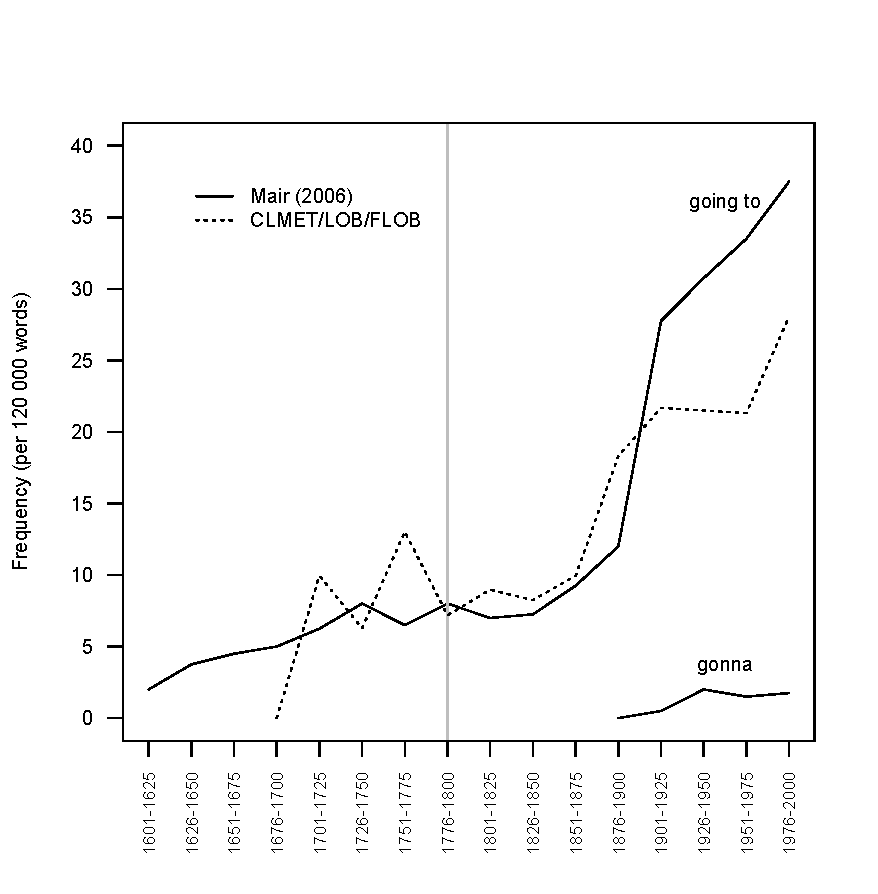
\includegraphics[width=.8\textwidth,keepaspectratio]{figures/goingtogrammaticalization}
\end{figure}

\begin{table}[!htbp]
\caption{Discourse frequency of \textit{going to}}
\label{tab:corpusgoingto}
\begin{tabular}[t]{c S[table-format=2] S[table-format=7] S l}
\lsptoprule
\multicolumn{1}{l}{\makecell[b]{Period \\ starting}} & \multicolumn{1}{l}{\makecell[b]{Raw \\ Freq.}} & \multicolumn{1}{l}{\makecell[b]{No. of \\ words}} & \multicolumn{1}{l}{\makecell[b]{Freq. p. \\ 120t words}} & \multicolumn{1}{l}{\makecell[b]{Data \\ Source}} \\
\midrule
1701 & 14 & 168799 & 9.95 & CLMET \\
1726 & 242 & 4623107 & 6.28 & CLMET \\
1751 & 591 & 5446006 & 13.02 & CLMET \\
1776 & 258 & 4308242 & 7.19 & CLMET \\
1801 & 231 & 3087842 & 8.98 & CLMET \\
1826 & 552 & 8024490 & 8.25 & CLMET \\
1851 & 442 & 5335906 & 9.94 & CLMET \\
1876 & 816 & 5349213 & 18.31 & CLMET \\
1901 & 722 & 3997155 & 21.68 & CLMET \\
1926 & & & 21.5 & (Extrapolated) \\
1951 & 180 & 1012985 & 21.32312 & LOB \\
1976 & 236 & 1009304 & 28.05894 & FLOB \\
\lspbottomrule
\end{tabular}
\end{table}

The grey line in Figure \ref{fig:mairgoingto} shows Mair's conservative estimate for the point at which the construction was firmly established as a way to express future tense. As the results from the OED \is{OED} citations and from the corpora show, there was only a small rise in frequency \is{frequency} during the time that the construction became established, but a substantial jump in frequency afterwards. Interestingly, around the time of that jump, we also find the first documented instances of the contracted form \textit{gonna} (from Mair's data -- the contracted form is not frequent enough in the corpora used here to be shown). These results suggest that semantic \is{semantics} reanalysis is the first step in grammaticalization, \is{grammaticalization} followed by a rise in discourse frequency \is{frequency} accompanied by phonological reduction.

This case study demonstrates that very large \is{corpus size} collections of citations can indeed be used as a corpus, as long as we are investigating phenomena that are likely to occur in citations collected to illustrate other phenomena; the results are very similar to those we get from well\hyp{}constructed linguistic corpora. The case study also demonstrates the importance of corpora in diachronic \is{diachrony} research, a field of study which, as mentioned in Chapter \ref{ch:needforcorpus} has always relied on citations drawn from authentic \is{authenticity} texts, but which can profit from querying \is{query} large \is{corpus size} collections of such texts and quantifying \is{quantitative research} the results.

\subsection{Grammar and cultural analysis}
\label{sec:grammarandculturalanalysis}

Like words, grammatical \is{grammar} structures usually represent themselves in corpus linguistic studies -- they are either investigated as part of a description \is{description} of the syntactic \is{syntax} behavior of lexical items or they are investigated in their own right in order to learn something about their semantic, \is{semantics} formal or functional restrictions. However, like words, they can also be used as representatives \is{representativeness} of some aspect of the speech community's culture, \is{culture} specifically, a particular culturally defined scenario. To take a simple example: if we want to know what kinds of things are transferred between people in a given culture, we may look at the theme arguments of ditransitive \is{ditransitivity} constructions in a large \is{corpus size} corpus; we may look for collocates \is{collocation} in the verb \is{verb} and theme positions of the ditransitive if we want to know \textit{how} particular things are transferred \citep[cf.][]{ludeling_corpora_2009}. In this way, grammatical \is{grammar} structures can become diagnostics of culture. \is{culture} Again, care must be taken to ensure that the link between a grammatical structure and a putative scenario is plausible.

\subsubsection{Case study: He said, she said}
\label{sec:hesaidshesaid}

In a paper on the medial representation of men and women, \is{gender stereotypes} \citet{caldas-coulthard_discourse_1993} finds that men are quoted vastly more frequently than women in the COBUILD corpus (cf. also Chapter \ref{ch:morphology}). She also notes in passing that the verbs \is{verb} of communication used to introduce or attribute the quotes differ -- both men's and women's speech is introduced using general verbs of communication, such as \textit{say} or \textit{tell}, but with respect to more descriptive verbs, there are differences: ``Men \textit{shout} and \textit{groan}, while women (and children) \textit{scream } and \textit{yell}'' \citep[204]{caldas-coulthard_discourse_1993}.

The construction [QUOTE + Subj + V] is a perfect example of a diagnostic for a cultural \is{culture} frame: it is routinely used (in written \is{medium} language) to describe a speech event. Crucially, the verb \is{verb} slot offers an opportunity to introduce additional information (such as the manner of speaking, as in the examples of manner verbs verbs just mentioned (that often contain evaluations), but also the type of speech act being performed (\textit{ask}, \textit{order}, etc.). It is also easy to find even in an untagged \is{POS tagging} corpus, since it includes (by definition) a passage of direct speech surrounded by quotation marks, a subject that is, in an overwhelming number of cases, a pronoun, \is{pronoun} and a verb (or verb \is{verb} group) -- typically in that order. In a written \is{medium} corpus, we can thus query the sequence $\langle$ \texttt{[word="{''}"] [pos="pronoun"] [pos="verb"]} $\rangle$ to find the majority of examples of the construction. In order to study differences in the representation of men and women, \is{gender stereotypes} we can query the pronouns \textit{he} and \textit{she} separately to obtain representative \is{representativeness} samples of male and female speech act events without any annotation. \is{annotation}

\begin{table}[!htbp]
\caption{Verbal collexemes of [QUOTE + Pron + V] (BNC)}
\label{tab:quotecollexemes}
\resizebox{\textwidth}{!}{%
\begin{tabular}[t]{l *{2}{S[table-format=4]} *{2}{S[table-format=8]} S}
\lsptoprule
\multicolumn{1}{c}{\makecell[tc]{\textvv{Verb}}} & \multicolumn{1}{c}{\makecell[tc]{Frequency with \\ \textvv{male subjects}}} & \multicolumn{1}{c}{\makecell[tc]{Frequency with \\ \textvv{female subjects}}} & \multicolumn{1}{c}{\makecell[tc]{Other words w. \\ \textvv{male subjects}}} & \multicolumn{1}{c}{\makecell[tc]{Other words w. \\ \textvv{female subjects}}} & \multicolumn{1}{c}{\makecell[tc]{G\textsuperscript{2}}} \\
\midrule
\multicolumn{6}{l}{Most strongly associated with \textvv{male subjects}} \\
\midrule
\textit{say} & 19301 & 11710 & 34916 & 26180 & 221.113740025537 \\
\textit{growl} & 158 & 5 & 54059 & 37885 & 131.833639357989 \\
\textit{drawl} & 172 & 10 & 54045 & 37880 & 122.790669077291 \\
\textit{write} & 239 & 56 & 53978 & 37834 & 66.2703036146206 \\
\textit{grate} & 80 & 4 & 54137 & 37886 & 59.7784278533784 \\
\textit{grin} & 301 & 89 & 53916 & 37801 & 58.4376336066056 \\
\textit{add} & 1526 & 771 & 52691 & 37119 & 57.0358747668258 \\
\textit{rasp} & 78 & 7 & 54139 & 37883 & 46.7825983195404 \\
\textit{continue} & 368 & 140 & 53849 & 37750 & 40.8160058329648 \\
\textit{snarl} & 82 & 13 & 54135 & 37877 & 34.1922679841907 \\
\textit{roar} & 54 & 5 & 54163 & 37885 & 31.88983015266 \\
\textit{chuckle} & 113 & 28 & 54104 & 37862 & 28.9961524072897 \\
\textit{murmur} & 633 & 311 & 53584 & 37579 & 27.1042800738047 \\
\textit{comment} & 117 & 34 & 54100 & 37856 & 23.3699450627582 \\
\textit{shout} & 349 & 155 & 53868 & 37735 & 23.3398935606577 \\
\textit{gesture} & 93 & 24 & 54124 & 37866 & 22.4960822128815 \\
\textit{grunt} & 51 & 8 & 54166 & 37882 & 21.4475135121844 \\
\textit{boom} & 26 & 1 & 54191 & 37889 & 20.7846724511177 \\
\textit{wink} & 34 & 3 & 54183 & 37887 & 20.549582166759 \\
\textit{claim} & 69 & 16 & 54148 & 37874 & 19.3533927260091 \\
\midrule
\multicolumn{6}{l}{Most strongly associated with \textvv{female subjects}} \\
\midrule
\textit{whisper} & 393 & 666 & 53824 & 37224 & 205.213509030231 \\
\textit{cry} & 216 & 395 & 54001 & 37495 & 137.792857031815 \\
\textit{feel} & 94 & 206 & 54123 & 37684 & 92.8582736796259 \\
\textit{manage} & 32 & 116 & 54185 & 37774 & 85.5960328992645 \\
\textit{snap} & 174 & 275 & 54043 & 37615 & 73.8061205295948 \\
\textit{retort} & 75 & 155 & 54142 & 37735 & 64.5876647672653 \\
\textit{protest} & 60 & 136 & 54157 & 37754 & 63.8828166553974 \\
\textit{giggle} & 13 & 61 & 54204 & 37829 & 53.4026088768348 \\
\textit{try} & 85 & 152 & 54132 & 37738 & 50.9082148546456 \\
\textit{ask} & 2136 & 1860 & 52081 & 36030 & 49.9523882508786 \\
\textit{flush} & 5 & 41 & 54212 & 37849 & 46.5313347509488 \\
\textit{wail} & 8 & 46 & 54209 & 37844 & 44.9207452054127 \\
\textit{swallow} & 24 & 71 & 54193 & 37819 & 44.2276081076112 \\
\textit{gasp} & 69 & 125 & 54148 & 37765 & 42.7478681479244 \\
\textit{exclaim} & 137 & 196 & 54080 & 37694 & 42.4370037780204 \\
\textit{force} & 9 & 45 & 54208 & 37845 & 40.8456344052239 \\
\textit{flare} & 1 & 27 & 54216 & 37863 & 40.4086421411062 \\
\textit{hear} & 82 & 130 & 54135 & 37760 & 35.0120478684469 \\
\textit{sob} & 13 & 45 & 54204 & 37845 & 32.0195724567643 \\
\textit{blush} & 3 & 27 & 54214 & 37863 & 31.6506392273931 \\
\lspbottomrule
\multicolumn{6}{l}{\scriptsize{Supplementary Online Material: RLW8}} \\ %OSM
\end{tabular}}
\end{table}
% me: query: BNC; [word="(?|\")"] [word="(he|she)"%c][pos=".*VV.*"]; count Last by hw on match[1]..match[2]

This design \is{research design} can be applied deductively, \is{deduction} if we have hypotheses about the gender\hyp{}specific \is{gender stereotypes} usage of particular (sets of) verbs, \is{verb} or inductively, \is{induction} if we simply calculate the association \is{association} strength of all verbs to one pronoun \is{pronoun} as compared to the other. In either case we have two nominal \is{nominal data} variables, \textsc{Subject of Quoted Speech}, with the variables \textsc{male} (\textit{he}) and \textsc{female} (\textit{she}), and \textsc{Speech Activity Verb} with all occurring verbs \is{verb} as its values. Table \ref{tab:quotecollexemes} shows the results of an inductive \is{induction} application of the design \is{research design} to the BNC. \is{BNC}

There is a clear difference that corroborates Caldas\hyp{}Coulthard's casual observation: the top ten verbs \is{verb} of communication associated \is{association} with men contain five verbs conveying a rough, unpleasant and\slash or aggressive manner of speaking (\textit{growl}, \textit{grate}, \textit{rasp}, \textit{snarl}, \textit{roar}), while those for women only include one (\textit{snap}, related to irritability rather than outright aggression). \is{gender stereotypes} Interestingly, two very general communication verbs, \textit{say} and \textit{write}, are also typical for men's reported speech. Women's speech is introduced by verbs \is{verb} conveying weakness or communicative subordination (\textit{whisper}, \textit{cry}, \textit{manage}, \textit{protest}, \textit{wail} and \textit{deny}).

\subsection{Grammar and counterexamples}
\label{sec:grammarandcounterexamples}

While this book focuses on quantitative \is{quantitative research} designs, \is{research design} non\hyp{}quantitative \is{qualitative research} designs are possible within the general framework adopted. Chapter \ref{ch:scientificmethod} included a discussion of counterexamples \is{counterexample} and their place in a scientific framework for corpus linguistics. Let us conclude this chapter with a case study making use of them.

\subsubsection{Case study: \textit{To}- vs. \textit{that}-complements}
\label{sec:tovsthatcomplements}

A good case study for English that is based largely on counterexamples \is{counterexample} is \citet{rohdenburg_is_2003}, who looks at a number of claims made about the semantics \is{semantics} of infinitival complements \is{complementation} as compared to \textit{that}-clauses. He takes claims made by other authors based on their intuition \is{intuition} and treats them like Popperian hypotheses, searching the BNC \is{BNC} for counterexamples. He mentions more or less informal impressions about frequencies, but only to clarify that the counterexamples \is{counterexample} are not just isolated occurrences that could be explained away.

For example, he takes the well\hyp{}known claim that with verbs \is{verb} of knowing, infinitival complements \is{complementation} present knowledge as subjective\slash personal, while \textit{that-}clauses present knowledge as objective\slash impersonal\slash public. This is supposed to explain acceptability \is{acceptability} judgments like the following (\citealt[45--46]{corum_be_1973}, \citealt[50, 136]{wierzbicka_semantics_1988}):

\begin{exe}
\ex
\begin{xlist}
\label{ex:findtobe}
\ex He found her to be intelligent.
\ex[*]{I bet that if you look in the files, you'll find her to be Mexican.}
\ex I bet that if you look in the files, you'll find that she is Mexican.
\end{xlist}
\end{exe}

The crucial counterexample \is{counterexample} here would be one like (\ref{ex:findtobe}b), with an infinitival complement \is{complementation} that expresses knowledge that is ``public'' rather than ``personal\slash experiential''; also of interest would be examples with \textit{that}-clauses that express personal\slash experiential knowledge. The corresponding queries are easy enough to define:

\begin{exe}
\ex
\begin{xlist}
\label{ex:findtobequery}
\ex \begin{minipage}[t]{0.85\textwidth} \raggedright \texttt{[word="(find|\allowbreak finds|\allowbreak finding|\allowbreak found)"\%c]} \texttt{[word="(me|\allowbreak you|\allowbreak him|\allowbreak her|\allowbreak it|\allowbreak us|\allowbreak them)"\%c]} \texttt{[word="to"\%c]} \texttt{[word="be"\%c]} \end{minipage}
\ex \begin{minipage}[t]{0.85\textwidth} \raggedright \texttt{[word="(find|\allowbreak finds|\allowbreak finding|\allowbreak found)"\%c]} \texttt{[word="that"\%c]} \texttt{[word="(I|\allowbreak you|\allowbreak he|\allowbreak she|\allowbreak it|\allowbreak we|\allowbreak they)"\%c]} \texttt{[word="(is|\allowbreak are|\allowbreak was|\allowbreak were)"\%c]} \end{minipage}
\end{xlist}
\end{exe}

This query follows the specific example in (\ref{ex:findtobe}b) very narrowly -- we could, of course, define a broader one that would capture, \is{retrieval} for example, proper names and noun \is{noun} phrases in addition to pronouns. \is{pronoun} But remember that we are looking for counterexamples, \is{counterexample} and if we can find these with a query following the structure of supposedly non\hyp{}acceptable \is{acceptability} sentences very closely, they will be all the more convincing.

The BNC \is{BNC} contains not just one, but many counterexamples. \is{counterexample} Here are some examples with \textit{that}-complements \is{complementation} expressing subjective, personal knowledge:

\begin{exe}
\ex
\begin{xlist}
\label{ex:findthatsubjective}
\ex Erika was surprised to find that she was beginning to like Bach (BNC A7A)
\ex $[$A$]$che of loneliness apart, I found that I was stimulated by the challenge of finding my way about this great and beautiful city. (BNC AMC)
\end{xlist}
\end{exe}

And here are some with \textit{to}-complements \is{complementation} expressing objective, impersonal knowledge:

\begin{exe}
\ex
\begin{xlist}
\label{ex:findtobefact}
\ex Li and her coworkers have been able to locate these sequence variations ... in the three\hyp{}dimensional structure of the toxin, and found them to be concentrated in the $\beta$ sheets of domain II. (BNC ALV)
\ex The visiting party, who were the first and last ever to get a good look at the crater of Perboewetan, found it to be about \num{1000} metres in diameter and about fifty metres deep. (BNC ASR)
\end{xlist}
\end{exe}

These counterexamples \is{counterexample} (and others not cited here) in fact give us a new hypothesis as to what the specific semantic \is{semantics} contribution of the \textit{to}-complement \is{complementation} may be: if used to refer to objective knowledge, it overwhelmingly refers to situations where this objective knowledge was not previously known to the participants of the situation described. In fact, if we extend our search for counterexamples \is{counterexample} beyond the BNC \is{BNC} to the world\hyp{}wide web, we find examples that are even more parallel to (\ref{ex:findtobe}b), such as (\ref{ex:findtobenationality}), all produced by native speakers of English:

\begin{exe}
\ex
\begin{xlist}
\label{ex:findtobenationality}
\ex Afterwards found that French had stopped ship and found her to be German masquerading as Greek. (www.hmsneptune.com)
\ex I was able to trace back my Grandfathers name ... to Scotland and then into Sussex and Surrey, England. Very exciting! Reason being is because we were told that the ancestors were Irish and we found them to be Scottish! (www.gettheeblowdryer.com)
\ex Eishaus -- This place is an Erlangen institution, should you ever get to meet the owner you'll find him to be American, he runs this wonderful ice cream shop as his summer job away from his `proper' job in the states. (theerlangenexpat.wordpress.com)
\end{xlist}
\end{exe}

Again, what is different in these examples from the (supposedly unacceptable) example (\ref{ex:findtobe}b) is that the knowledge in question is new (and surprising) to the participants of the situation -- a seemingly Greek ship turning out to be German, a supposedly Irish ancestor turning out to be Scottish, and the proprietor of an ice\hyp{}cream shop in the small Bavarian town of Erlangen turning out to be American.

This observation could now be used as the basis for a new hypothesis concerning the difference between the two constructions, but even if it is not or if this hypothesis turned out to be false, the counterexamples \is{counterexample} clearly disprove the claim by Wierzbicka and others concerning the subjective\slash objective distinction (\citealt{rohdenburg_is_2003} actually goes on to propose an information\hyp{}structural account of the difference between the \textit{to-} and the \textit{that}-complement). \is{complementation}

This case study was intended to show how counterexamples \is{counterexample} may play a role in disproving hypotheses based on introspection \is{introspection} and constructed examples (see \citealt{meurers_use_2005} and \citealt{meurers_corpora_2009} as good examples for the theoretically informed search for counterexamples).

\chapter{Morphology}
\label{ch:morphology}

We saw in Chapter \ref{ch:grammar} \is{grammar} that the wordform\hyp{}centeredness of most corpora and corpus\hyp{}access tools requires a certain degree of ingenuity when studying structures larger than the word. It does not pose particular problems for corpus\hyp{}based morphology, \is{morphology} which studies structures smaller than the word. Corpus morphology is mostly concerned with the distribution \is{distribution, conditional} of affixes, \is{affix} and retrieving \is{retrieval} all occurrences of an affix \is{affix} plausibly starts with the retrieval of all strings potentially containing this affix. \is{affix} \is{affix} We could retrieve all occurrences of \textit{-ness}, for example, with a query like $\langle$ \texttt{[word=".+ness(es)?"\%c]} $\rangle$. The recall \is{recall} of this query will be close to 100 percent, as all words containing the suffix \textit{-ness} end in the string \texttt{ness}, optionally followed by the string \texttt{es} in the case of plurals. \is{number} Depending on the tokenization \is{tokenization} of the corpus, this query might miss cases where the word containing the suffix \textit{-ness} is the first part of a hyphenated compound, such as \textit{usefulness-rating} or \textit{consciousness-altering}; we could alter the query to something like $\langle$ \texttt{[word=".+ness(es)?(--.+=)?"\%c]} $\rangle$ if we believe that including these cases in our sample is crucial. The precision \is{precision} of such a query will not usually be 100 percent, as it will also retrieve words that accidentally happen to end with the string specified in our query -- in the case of \textit{-ness}, these would be words like \textit{witness}, \textit{governess} or place names like \textit{Inverness}. The degree of precision will depend on how unique the string in our query is for the affix \is{affix} in question; for \textit{-ness} and \textit{-ity} it is fairly high, as there are only a few words that share the same string accidentally (examples like those just mentioned for \textit{-ness} and words like \textit{city} and \textit{pity} for \textit{-ity}), for a suffix \is{affix} like \textit{-ess} (``female animate entity'') it is quite low, as a query like $\langle$ \texttt{[word=".+ess(es)?"\%c]} $\rangle$ will also retrieve \is{retrieval} all words with the suffixes \is{affix} \textit{-ness} and \textit{-less}, as well as many words whose stem \is{statistics} ends in \textit{ess}, like \textit{process}, \textit{success}, \textit{press}, \textit{access}, \textit{address}, \textit{dress}, \textit{guess} and many more.

However, once we have extracted \is{retrieval} and -- if necessary -- manually \is{manual analysis} cleaned up our data set, we are faced with a problem that does not present itself when studying lexis or grammar: \is{grammar} the very fact that affixes \is{affix} do not occur independently but always as parts of words, some of which (like \textit{wordform-centeredness} in the first sentence of this chapter) have been created productively \is{productivity} on the fly for a specific purpose, while others (like \textit{ingenuity} in the same sentence) are conventionalized \is{conventionality} lexical items that are listed in dictionaries, \is{dictionary} even though they are theoretically the result of attaching an affix \is{affix} to a known stem \is{statistics} (like \textit{ingen-}, also found in \textit{ingenious} and, confusingly, its almost\hyp{}antonym \is{antonymy} \textit{ingenuous}). We have to keep the difference between these two kinds of words in mind when constructing morphological \is{morphology} research designs; \is{research design} since the two kinds are not always clearly distinguishable, this is more difficult than it sounds. Also, the fact that affixes \is{affix} always occur as parts of words has consequences for the way we can, and should, count them; in quantitative \is{quantitative research} corpus\hyp{}linguistics, this is a crucial point, so I will discuss it in quite some detail before we turn to our case studies.

\section{Quantifying morphological phenomena}
\label{sec:quantifyingmorphologicalphenomena}

\subsection{Counting morphemes: types, tokens and hapax legomena}
\label{sec:countingmorphemes}

Determining the frequency \is{frequency} of a linguistic phenomenon in a corpus or under a particular condition seems a straightforward task: we simply count the number of instances of this phenomenon in the corpus or under that condition. However, this sounds straightforward (in fact, tautological) only because we have made tacit assumptions about what it means to be an ``instance'' of a particular phenomenon.

When we are interested in the frequency \is{frequency} of occurrence of a particular word, it seems obvious that every occurrence of the word counts as an instance. In other words, if we know how often the word occurs in our data, we know how many instances there are in our data. For example, in order to determine the number of instances of the definite article \is{determiner} in the BNC, \is{BNC} we construct a query that will retrieve \is{retrieval} the string \texttt{the} in all combinations of upper and lower case letters, i.e. at least \textit{the}, \textit{The}, and \textit{THE}, but perhaps also \textit{tHe}, \textit{ThE}, \textit{THe}, \textit{tHE} and \textit{thE}, just to be sure). We then count the hits (since this string corresponds uniquely to the word \textit{the}, we don't even have to clean up the results manually). \is{manual analysis} The query will yield \num{6041234} hits, so there are \num{6041234} instances of the word \textit{the} in the BNC. \is{BNC}

When searching for grammatical \is{grammar} structures (for example in Chapters \ref{ch:quantifyingresearch} and \ref{ch:significancetesting}), simply transferred this way of counting occurrences. For example, in order to determine the frequency \is{frequency} of the \textit{s}-possessive \is{possessive} in the BNC, \is{BNC} we would define a reasonable query or set of queries (which, as discussed in various places in this book, can be tricky) and again simply count the hits. \is{hit} Let us assume that the query $\langle$ \texttt{[pos="(POS|DPS)"] [pos=".*AJ.*"]? [pos=".*NN.*"]} $\rangle$ is a reasonable approximation: it retrieves \is{retrieval} all instances of the possessive clitic \is{clitic} (tagged \texttt{POS} in the BNC) \is{BNC} or a possessive determiner \is{determiner} (\texttt{DPS}), optionally followed by a word tagged \is{POS tagging} as an adjective \is{adjective} (\texttt{AJ0}, \texttt{AJC} or \texttt{AJS}, even if it is part of an ambiguity \is{ambiguity} tag), followed by a word tagged as a noun \is{noun} (\texttt{NN0}, \texttt{NN1} or \texttt{NN2}, even if it is part of an ambiguity tag). This query will retrieve \num{1651908} hits, so it seems that there are \num{1651908} instances of the \textit{s}-possessive \is{possessive} in the BNC. \is{BNC}

However, there is a crucial difference between the two situations: in the case of the word \textit{the}, every instance is identical to all others (if we ignore upper and lower case). This is not the case for the \textit{s}-possessive. Of course, here, too, many instances are identical to other instances: there are exact repetitions of proper names, like \textit{King's Cross} (322 hits) or \textit{People's revolutionary party} (47), of (parts of) idiomatic \is{idiomaticity} expressions, like \textit{arm's length} (216) or \textit{heaven's sake} (187) or non\hyp{}idiomatic but nevertheless fixed phrases like \textit{its present form} (107) or \textit{child's best interest} (26), and also of many free combinations of words that recur because they are simply communicatively useful in many situations, like \textit{her head} (5105), \textit{his younger brother} (112), \textit{people's lives} (224) and \textit{body's immune system} (29).

This means that there are two different ways to count occurrences of the \textit{s}-possessive. \is{possessive} First, we could simply count all instances without paying any attention to whether they recur in identical form or not. When looking at occurrences of a linguistic item or structure in this way, they are referred to as \textit{tokens}, \is{token (instance)} so \num{1651908} is the \textit{token frequency} \is{frequency, token} of the possessive. Second, we could exclude repetitions and count only the number of instances that are different from each other, for example, we would count \textit{King's Cross} only the first time we encounter it, disregarding the other 321 occurrences. When looking at occurrences of linguistic items in this way, they are referred to as \textit{types}; \is{type (category)} the type frequency \is{frequency, type} of the \textit{s}-possessive \is{possessive} in the BNC \is{BNC} is \num{268450} (again, ignoring upper and lower case). The type frequency of \textit{the}, of course, is 1.

Let us look at one more example of the type\slash token \is{token (instance)} \is{type (category)} distinction before we move on. Consider the following famous line from the theme song of the classic television series ``Mister Ed'':

\begin{exe}
\ex A horse is a horse, of course, of course...
\label{ex:horseisahorse}
\end{exe}

At the word level, it consists of nine tokens \is{token (instance)} (if we ignore punctuation): \textit{a}, \textit{horse}, \textit{is}, \textit{a}, \textit{horse}, \textit{of}, \textit{course}, \textit{of}, and \textit{course}, but only of five types: \is{type (category)} \textit{a}, \textit{horse}, \textit{is}, \textit{of}, and \textit{course}. Four of these types occur twice, one (\textit{is}) occurs only once. At the level of phrase structure, it consists of seven tokens: the NPs \textit{a horse}, \textit{a horse}, \textit{course}, and \textit{course}, the PPs \textit{of course} and \textit{of course}, and the VP \textit{is a horse}, but only of three types: VP, NP and PP.

In other words, we can count ``instances'' at the level of types \is{type (category)} or at the level of tokens. \is{token (instance)} Which of the two levels is relevant in the context of a particular research design \is{research design} depends both on the kind of phenomenon we are counting and on our research question. When studying words, we will normally be interested in how often they are used under a particular condition, so it is their token \is{token (instance)} frequency \is{frequency, token} that is relevant to us; but we could imagine designs \is{research design} where we are mainly interested in whether a word occurs at all, in which case all that is relevant is whether its type \is{type (category)} frequency \is{frequency, type} is one or zero. When studying grammatical \is{grammar} structures, we will also mainly be interested in how frequently a particular grammatical structure is used under a certain condition, regardless of the words that fill this structure. Again, it is the token \is{token (instance)} frequency \is{frequency, token} that is relevant to us. However, note that we can (to some extent) ignore the specific words filling our structure only because we are assuming that the structure and the words are, in some meaningful sense, independent of each other; i.e., that the same words could have been used in a different structure (say, an \textit{of}-possessive \is{possessive} instead of an \textit{s}-possessive) or that the same structure could have been used with different words (e.g. \textit{John's spouse} instead of \textit{his wife}). Recall that in our case studies in Chapter \ref{ch:significancetesting} we excluded all instances where this assumption does not hold (such as proper names and fixed expressions); since there is no (or very little) choice with these cases, including them, let alone counting repeated occurrences of them, would have added nothing (we did, of course, include repetitions of free combinations, of which there were four in our sample: \textit{his staff}, \textit{his mouth}, \textit{his work} and \textit{his head} occurred twice each).

Obviously, instances of morphemes \is{morphology} (whether inflectional or derivational) can be counted in the same two ways. Take the following passage from William Shakespeare's play Julius Cesar:

\begin{exe}
\ex CINNA: ... Am I a married man, or a bachelor? Then, to answer every man directly and briefly, wisely and truly: wisely I say, I am a bachelor.
\label{ex:shakspearecinna}
\end{exe}

Let us count the occurrences of the adverbial \is{adverb} suffix \is{affix} \textit{-ly}. There are five word tokens \is{token (instance)} that contain this suffix \is{affix} (\textit{directly}, \textit{briefly}, \textit{wisely}, \textit{truly}, and \textit{wisely}), so its token frequency \is{frequency, token} is five; however, there are only four types, \is{type (category)} since \textit{wisely} occurs twice, so its type frequency \is{frequency, type} in this passage is four.

Again, whether type \is{type (category)} or token \is{token (instance)} frequency \is{frequency, token} is the more relevant or useful measure \is{measurement} depends on the research design, \is{research design} but the issue is more complicated than in the case of words and grammatical \is{grammar} structures. Let us begin to address this problem by looking at the diminutive affixes \is{affix} \textit{-icle} (as in \textit{cubicle}, \textit{icicle}) and \textit{mini-} (as in \textit{minivan}, \textit{mini\hyp{}cassette}).

\textit{a. Token frequency}. First, let us count the tokens \is{token (instance)} of both affixes \is{affix} in the BNC. \is{BNC} This is relatively easy in the case of \textit{-icle}, since the string \texttt{icle} is relatively unique to this morpheme \is{morphology} (the name \textit{Pericles} is one of the few false hits that the query $\langle$ \texttt{[word=".+icles?"\%c]} $\rangle$ will retrieve). \is{retrieval} It is more difficult in the case of \textit{mini-}, since there are words like \textit{minimal}, \textit{minister}, \textit{ministry}, \textit{miniature} and others that start with the string \texttt{mini} but do not contain the prefix \is{affix} \textit{mini-}. Once we have cleaned up our concordances \is{concordance} (available in the Supplementary Online Material, file LMY7), we will find that \textit{-icle} has a token frequency \is{frequency, token} of \num{20772} -- more than ten times that of \textit{mini-}, which occurs only \num{1702} times. We might thus be tempted to conclude that \textit{-icle} is much more important in the English language than \textit{mini-}, and that, if we are interested in English diminutives, we should focus on \textit{-icle}. However, this conclusion would be misleading, or at least premature, for reasons related to the problems introduced above.

Recall that affixes \is{affix} do not occur by themselves, but always as parts of words (this is what makes them affixes \is{affix} in the first place). This means that their token frequency \is{frequency, token} can reflect situations that are both quantitatively and qualitatively very different. Specifically, a high token frequency of an affix \is{affix} may be due to the fact that it is used in a small number of very frequent words, or in a large number of very infrequent words (or something in between). The first case holds for \textit{-icle}: the three most frequent words it occurs in (\textit{article}, \textit{vehicle} and \textit{particle}) account for \num{19195} hits (i.e., 92.41 percent of all occurrences). In contrast, the three most frequent words with \textit{mini-} (\textit{mini\hyp{}bus}, \textit{mini\hyp{}bar} and \textit{mini\hyp{}computer}) account for only 557 hits, i.e. 32.73 percent of all occurrences. To get to 92.4 percent, we would have to include the 253 most frequent words (roughly two thirds of all types). \is{type (category)}

In other words, the high token \is{token (instance)} frequency \is{frequency, token} of \textit{-icle} tells us nothing (or at least very little) about the importance of the affix; \is{affix} \is{affix} if anything, it tells us something about the importance of some of the words containing it. This is true regardless of whether we look at its token frequency in the corpus as a whole or under specific conditions; if its token frequency \is{frequency, token} turned out to be higher under one condition than under the other, this would point to the association \is{association} between that condition and one or more of the words containing the affix, \is{affix} rather than between the condition and the affix \is{affix} itself.

For example, the token frequency \is{frequency, token} of the suffix \is{affix} \textit{-icle} is higher in the BROWN \is{BROWN} corpus (269 tokens) than in the LOB \is{LOB} corpus (225 tokens). However, as Table \ref{tab:iclewords} shows, this is simply due to differences in the frequency of individual words -- the words \textit{particle} and \textit{vehicle} are substantially more frequent in the BROWN \is{BROWN} corpus, and while, conversely, \textit{article} is more frequent in the LOB \is{LOB} corpus, it cannot make up for the difference. As the $\chi^2$ \is{chi-square test} components show, the difference in frequency of some of the individual words is even statistically significant, but nothing follows from this with respect to the suffix \is{affix} \textit{-icle}.

\begin{table}[!htbp]
\caption{Words containing \textit{-icle} in two corpora}
\label{tab:iclewords}
\resizebox*{!}{\textheight}{%
\begin{tabular}[t]{lccr}
\lsptoprule
 & \multicolumn{2}{c}{\textvv{Corpus}} & \\
\textvv{Word} & \textvv{lob} & \textvv{brown} & Total \\
\midrule
\textit{\makecell[tl]{article}}
	& \makecell[t]{\begin{tabular}[t]{lS[table-format=2.2]} \small{\textit{Obs.:}} & 126 \\ \small{\textit{Exp.:}} & 102.48 \\ \small{\textit{$\chi^2$:}} & 5.40 \end{tabular}}
	& \makecell[t]{\begin{tabular}[t]{lS[table-format=2.2]} \small{\textit{Obs.:}} & 99 \\ \small{\textit{Exp.:}} & 122.52 \\ \small{\textit{$\chi^2$:}} & 4.52 \end{tabular}}
	& 225 \\[1.1cm]
\textit{\makecell[tl]{particle}}
	& \makecell[t]{\begin{tabular}[t]{lS[table-format=2.2]} \small{\textit{Obs.:}} & 38 \\ \small{\textit{Exp.:}} & 46.46 \\ \small{\textit{$\chi^2$:}} & 1.54 \end{tabular}}
	& \makecell[t]{\begin{tabular}[t]{lS[table-format=2.2]} \small{\textit{Obs.:}} & 64 \\ \small{\textit{Exp.:}} & 55.54 \\ \small{\textit{$\chi^2$:}} & 1.29 \end{tabular}}
	& 102 \\[1.1cm]
\textit{\makecell[tl]{vehicle}}
	& \makecell[t]{\begin{tabular}[t]{lS[table-format=2.2]} \small{\textit{Obs.:}} & 39 \\ \small{\textit{Exp.:}} & 57.84 \\ \small{\textit{$\chi^2$:}} & 6.14 \end{tabular}}
	& \makecell[t]{\begin{tabular}[t]{lS[table-format=2.2]} \small{\textit{Obs.:}} & 88 \\ \small{\textit{Exp.:}} & 69.16 \\ \small{\textit{$\chi^2$:}} & 5.13 \end{tabular}}
	& 127 \\[1.1cm]
\textit{\makecell[tl]{chronicle}}
	& \makecell[t]{\begin{tabular}[t]{lS[table-format=2.2]} \small{\textit{Obs.:}} & 7 \\ \small{\textit{Exp.:}} & 6.38 \\ \small{\textit{$\chi^2$:}} & 0.06 \end{tabular}}
	& \makecell[t]{\begin{tabular}[t]{lS[table-format=2.2]} \small{\textit{Obs.:}} & 7 \\ \small{\textit{Exp.:}} & 7.62 \\ \small{\textit{$\chi^2$:}} & 0.05 \end{tabular}}
	& 14 \\[1.1cm]
\textit{\makecell[tl]{ventricle}}
	& \makecell[t]{\begin{tabular}[t]{lS[table-format=2.2]} \small{\textit{Obs.:}} & 8 \\ \small{\textit{Exp.:}} & 5.47 \\ \small{\textit{$\chi^2$:}} & 1.18 \end{tabular}}
	& \makecell[t]{\begin{tabular}[t]{lS[table-format=2.2]} \small{\textit{Obs.:}} & 4 \\ \small{\textit{Exp.:}} & 6.53 \\ \small{\textit{$\chi^2$:}} & 0.98 \end{tabular}}
	& 12 \\[1.1cm]
\textit{\makecell[tl]{auricle}}
	& \makecell[t]{\begin{tabular}[t]{lS[table-format=2.2]} \small{\textit{Obs.:}} & 5 \\ \small{\textit{Exp.:}} & 2.28 \\ \small{\textit{$\chi^2$:}} & 3.26 \end{tabular}}
	& \makecell[t]{\begin{tabular}[t]{lS[table-format=2.2]} \small{\textit{Obs.:}} & 0 \\ \small{\textit{Exp.:}} & 2.72 \\ \small{\textit{$\chi^2$:}} & 2.72 \end{tabular}}
	& 5 \\[1.1cm]
\textit{\makecell[tl]{fascicle}}
	& \makecell[t]{\begin{tabular}[t]{lS[table-format=2.2]} \small{\textit{Obs.:}} & 0 \\ \small{\textit{Exp.:}} & 1.37 \\ \small{\textit{$\chi^2$:}} & 1.37 \end{tabular}}
	& \makecell[t]{\begin{tabular}[t]{lS[table-format=2.2]} \small{\textit{Obs.:}} & 3 \\ \small{\textit{Exp.:}} & 1.63 \\ \small{\textit{$\chi^2$:}} & 1.14 \end{tabular}}
	& 3 \\[1.1cm]
\textit{\makecell[tl]{testicle}}
	& \makecell[t]{\begin{tabular}[t]{lS[table-format=2.2]} \small{\textit{Obs.:}} & 0 \\ \small{\textit{Exp.:}} & 0.91 \\ \small{\textit{$\chi^2$:}} & 0.91 \end{tabular}}
	& \makecell[t]{\begin{tabular}[t]{lS[table-format=2.2]} \small{\textit{Obs.:}} & 2 \\ \small{\textit{Exp.:}} & 1.09 \\ \small{\textit{$\chi^2$:}} & 0.76 \end{tabular}}
	& 2 \\[1.1cm]
\textit{\makecell[tl]{conventicle}}
	& \makecell[t]{\begin{tabular}[t]{lS[table-format=2.2]} \small{\textit{Obs.:}} & 1 \\ \small{\textit{Exp.:}} & 0.46 \\ \small{\textit{$\chi^2$:}} & 0.65 \end{tabular}}
	& \makecell[t]{\begin{tabular}[t]{lS[table-format=2.2]} \small{\textit{Obs.:}} & 0 \\ \small{\textit{Exp.:}} & 0.54 \\ \small{\textit{$\chi^2$:}} & 0.54 \end{tabular}}
	& 1 \\[1.1cm]
\textit{\makecell[tl]{cuticle}}
	& \makecell[t]{\begin{tabular}[t]{lS[table-format=2.2]} \small{\textit{Obs.:}} & 1 \\ \small{\textit{Exp.:}} & 0.46 \\ \small{\textit{$\chi^2$:}} & 0.65 \end{tabular}}
	& \makecell[t]{\begin{tabular}[t]{lS[table-format=2.2]} \small{\textit{Obs.:}} & 0 \\ \small{\textit{Exp.:}} & 0.54 \\ \small{\textit{$\chi^2$:}} & 0.54 \end{tabular}}
	& 1 \\[1.1cm]
\textit{\makecell[tl]{canticle}}
	& \makecell[t]{\begin{tabular}[t]{lS[table-format=2.2]} \small{\textit{Obs.:}} & 0 \\ \small{\textit{Exp.:}} & 0.46 \\ \small{\textit{$\chi^2$:}} & 0.46 \end{tabular}}
	& \makecell[t]{\begin{tabular}[t]{lS[table-format=2.2]} \small{\textit{Obs.:}} & 1 \\ \small{\textit{Exp.:}} & 0.54 \\ \small{\textit{$\chi^2$:}} & 0.38 \end{tabular}}
	& 1 \\[1.1cm]
\textit{\makecell[tl]{icicle}}
	& \makecell[t]{\begin{tabular}[t]{lS[table-format=2.2]} \small{\textit{Obs.:}} & 0 \\ \small{\textit{Exp.:}} & 0.46 \\ \small{\textit{$\chi^2$:}} & 0.46 \end{tabular}}
	& \makecell[t]{\begin{tabular}[t]{lS[table-format=2.2]} \small{\textit{Obs.:}} & 1 \\ \small{\textit{Exp.:}} & 0.54 \\ \small{\textit{$\chi^2$:}} & 0.38 \end{tabular}}
	& 1 \\[1.1cm]
\midrule
Total
	& \makecell[t]{225}
	& \makecell[t]{269}
	& \makecell[t]{494} \\
\lspbottomrule
\end{tabular}}
\end{table}
% me: query: [word=".+icles?"%c];
% me: false hits: LOB/BROWN: Pericles, BROWN: sticle
% me: lemmatized: a-particle, wave-particle

Even if all words containing a particular affix \is{affix} were more frequent under one condition (e.g. in one variety) \is{language variety} than under another, this would tell us nothing certain about the affix \is{affix} itself: while such a difference in frequency \is{frequency} could be due to the affix \is{affix} itself (as in the case of the adverbial \is{adverb} suffix \is{affix} \textit{-ly}, which is disappearing from American \is{American English} English, but not from British \is{British English} English), it could also be due exclusively to the words containing the affix. \is{affix}

This is not to say that the token \is{token (instance)} frequencies \is{frequency, token} of affixes \is{affix} can never play a useful role; they may be of interest, for example, in cases of morphological \is{morphology} alternation \is{alternation} (i.e. two suffixes \is{affix} competing for the same stems, \is{statistics} such as \textit{-ic} and \textit{-ical} in words like \textit{electric}\slash \textit{al}); here, we may be interested in the quantitative association \is{association} between particular stems and one or the other of the affix \is{affix} variants, essentially giving us a collocation\hyp{}like \is{collocation} research design \is{research design} based on token frequencies. \is{frequency, token} But for most research questions, the distribution \is{distribution, conditional} of token frequencies under different conditions is meaningless.

\textit{b. Type frequency}. In contrast, the type \is{type (category)} frequency \is{frequency, type} of an affix \is{affix} is a fairly direct reflection of the importance of the affix \is{affix} for the lexicon \is{lexicon} of a language: obviously an affix \is{affix} that occurs in many different words is more important than one that occurs only in a few words. Note that in order to compare type frequencies, we have to correct for the size \is{corpus size} of the sample: all else being equal, a larger sample will contain more types than a smaller one simply because it offers more opportunities for different types \is{type (category)} to occur (a point we will return to in more detail in the next subsection). A simple way of doing this is to divide the number of types by the number of tokens; \is{token (instance)} the resulting measure is referred to very transparently as the ``type\slash token ratio'' (or TTR): \is{type-token ratio}

\begin{exe}
\ex $\displaystyle{TTR = \frac{n \left( types \right) }{n \left( tokens \right)}}$
\label{ex:ttrformula}
\end{exe}

The TTR \is{type-token ratio} is the percentage of types \is{type (category)} in a sample are different from each other; or, put differently, it is the mean \is{mean} probability \is{probability} that we will encounter a new type if we go through the sample item by item.

For example, the affix \is{affix} \textit{-icle} occurs in just 31 different words in the BNC, \is{BNC} so its TTR \is{type-token ratio} is $\nicefrac{31}{20772} = 0.0015$. In other words, 0.15 percent of its tokens in the BNC are different from each other, the vast remainder consists of repetitions. Put differently, if we go through the occurrences of \textit{-icle} in the BNC \is{BNC} item by item, the probability \is{probability} that the next item instantiating this suffix \is{affix} will be a type \is{type (category)} we have not seen before is 0.15 percent, so we will encounter a new type on average once every 670 words. For \textit{mini-}, the type\hyp{}token \is{type-token ratio} ratio is much higher: it occurs in 382 different words, so its TTR is $\nicefrac{382}{1702} = 0.2244$. In other words, almost a quarter of all occurrences of \textit{mini-} are different from each other. Put differently, if we go through the occurrences of \textit{mini-} in the BNC \is{BNC} word by word, the probability \is{probability} that the next instance is a new type would be 22.4 percent, so we will encounter a new type \is{type (category)} about every four to five hits. \is{hit} The differences in their TTRs \is{type-token ratio} suggests that \textit{mini-}, in its own right, is much more central in the English lexicon \is{lexicon} than \textit{-icle}, even though the latter has a much higher token frequency. \is{frequency, token} Note that this is a statement only about the affixes; \is{affix} it does not mean that the \textit{words} containing \textit{mini-} are individually or collectively more important than those containing \textit{-icle} (on the contrary: words like \textit{vehicle}, \textit{article} and \textit{particle} are arguably much more important than words like \textit{minibus}, \textit{minicomputer} and \textit{minibar}).

Likewise, observing the type frequency \is{frequency, type} (i.e. the TTR) \is{type-token ratio} of an affix \is{affix} under different conditions provides information about the relationship between these conditions and the affix \is{affix} itself, albeit one that is mediated by the lexicon: \is{lexicon} it tells us how important the suffix \is{affix} in question is for the subparts of the lexicon that are relevant under those conditions. For example, there are 7 types \is{type (category)} and 9 tokens \is{token (instance)} for \textit{mini-} in the 1991 British \is{British English} FLOB \is{FLOB} corpus (two tokens each for \textit{mini\hyp{}bus} and \textit{mini\hyp{}series} and one each for \textit{mini\hyp{}charter}, \textit{mini\hyp{}disc}, \textit{mini\hyp{}maestro}, \textit{mini\hyp{}roll} and \textit{mini\hyp{}submarine}), so the TTR is $\nicefrac{7}{9} = 0.7779$. In contrast, in the 1991 US\hyp{}American \is{American English} FROWN \is{FROWN} corpus, there are 11 types and 12 tokens (two tokens for \textit{mini\hyp{}jack}, and one token each for \textit{mini\hyp{}cavalry}, \textit{mini\hyp{}cooper}, \textit{mini\hyp{}major}, \textit{mini\hyp{}retrospective}, \textit{mini\hyp{}version}, \textit{mini\hyp{}boom}, \textit{mini\hyp{}camp}, \textit{mini\hyp{}grinder}, \textit{mini\hyp{}series}, and \textit{mini\hyp{}skirt}), so the TTR \is{type\hyp{}token ratio} is $\nicefrac{11}{12} = 0.9167$. This suggests that the prefix \is{affix} \textit{mini-} was more important to the US\hyp{}English lexicon \is{lexicon} than to the British \is{British English} English lexicon in the 1990s, although, of course, the samples and the difference between them are both rather small, so we would not want to draw that conclusion without consulting larger \is{corpus size} corpora and, possibly, testing for significance first (a point I will return to in the next subsection).

\textit{c. Hapax legomena}. \is{hapax legomenon} While type frequency \is{frequency, type} is a useful way of measuring \is{measurement} the importance of affixes \is{affix} in general or under specific conditions, it has one drawback: it does not tell us whether the affix \is{affix} plays a productive \is{productivity} role in a language at the time from which we take our samples (i.e. whether speakers at that time made use of it when coining new words). An affix \is{affix} may have a high TTR \is{type\hyp{}token ratio} because it was productively used at the time of the sample, or because it was productively used at some earlier period in the history of the language in question. In fact, an affix \is{affix} can have a high TTR even if it was never productively \is{productivity} used, for example, because speakers at some point borrowed a large number of words containing it; this is the case for a number of Romance affixes \is{affix} in English, occurring in words borrowed from Norman French but never (or very rarely) used to coin new words. An example is the suffix \is{affix}
\textit{-ence}\slash \textit{-ance} occurring in many Latin and French loanwords (such as \textit{appearance}, \textit{difference}, \textit{existence}, \textit{influence}, \textit{nuisance}, \textit{providence}, \textit{resistance}, \textit{significance}, \textit{vigilance}, etc.), but only in a handful of words formed in English (e.g. \textit{abidance}, \textit{forbearance}, \textit{furtherance}, \textit{hinderance}, and \textit{riddance}).

In order to determine the productivity \is{productivity} (and thus the current importance) of affixes \is{affix} at a particular point in time, Harald Baayen (cf. e.g. \citealt{baayen_41._2009} for an overview) has suggested that we should focus on types \is{type (category)} that only occur once in the corpus, so\hyp{}called \textit{hapax legomena} \is{hapax legomenon} (Greek for `said once'). The assumption is that productive \is{productivity} uses of an affix \is{affix} (or other linguistic rule) should result in one\hyp{}off coinages (some of which may subsequently spread through the speech community while others will not).

Of course, not all hapax \is{hapax legomenon} legomena are the result of productive rule\hyp{}application: the words \textit{wordform\hyp{}centeredness} and \textit{ingenuity} that I used in the first sentence of this chapter are both hapax legomena in this book (or would be, if I did not keep mentioning them). However, \textit{wordform\hyp{}centeredness} is a word I coined productively \is{productivity} and which is (at the time of writing) not documented anywhere outside of this book; in fact, the sole reason I coined it was in order to use it as an example of a hapax \is{hapax legomenon} legomenon later). In contrast, \textit{ingenuity} has been part of the English language for more than four\hyp{}hundred years (the OED \is{OED} first records it in 1598); it occurs only once in this book for the simple reason that I only needed it once (or pretended to need it, to have another example of a hapax legomenon). So a word may be a hapax \is{hapax legomenon} legomenon because it is a productive \is{productivity} coinage, or because it is infrequently needed (in larger \is{corpus size} corpora, the category of hapaxes typically also contains misspelled or incorrectly tokenized \is{tokenization} words which will have to be cleaned up manualy \is{manual analysis} -- for example, the token \textit{manualy} is a hapax legomenon in this book because I just misspelled it intentionally, but the word \textit{manually} occurs dozens of times in this book).

Baayen's idea is quite straightforwardly to use the phenomenon of ``hapax \is{hapax legomenon} legomenon'' as an operationalization \is{operationalization} of the construct ``productive \is{productivity} application of a rule'' in the hope that the correlation between the two notions (in a large \is{corpus size} enough corpus) will be substantial enough for this operationalization to make sense.\footnote{Note also that the productive application of a suffix \is{affix} does not necessarily result in a hapax \is{hapax legomenon} legomenon: two or more speakers may arrive at the same coinage, or a single speaker may like their own coinage so much that they use it again; some researchers therefore suggest that we should also pay attention to ``dis legomena'' (words occurring twice) or even ``tris legomena'' (words occurring three times). We will stick with the mainstream here and use only hapax legomena.}

Like the number of types, \is{type (category)} the number of hapax \is{hapax legomenon} legomena is dependent on sample size \is{corpus size} (although the relationship is not as straightforward as in the case of types, see next subsection); it is useful, therefore, to divide the number of hapax legomena by the number of tokens \is{token (instance)} to correct for sample size:

\begin{exe}
\ex $\displaystyle{HTR = \frac{n \left( {hapax\ legomena} \right)}{n \left( {tokens} \right)}}$
\label{ex:htrformula}
\end{exe}
% me-layout: make sure text renders nicely in formula

We will refer to this measure as the hapax\hyp{}token \is{hapax-token ratio} ratio (or HTR) by analogy with the term \textit{type-token ratio}. \is{type-token ratio} Note, however, that in the literature this measure is referred to as \textit{P} for ``Productivity'' \is{productivity} (following Baayen, who first suggested the measure); I depart from this nomenclature here to avoid confusion with \textit{p} for ``probability (of error)''.

Let us apply this measure to our two diminutive affixes. \is{affix} The suffix \textit{-icle} has just five hapax legomena in the BNC \is{BNC} (\textit{auricle}, \textit{denticle}, \textit{pedicle}, \textit{pellicle} and \textit{tunicle}). This means that its HTR \is{hapax-token ratio} is $\nicefrac{5}{20772} = 0.0002$, so 0.02 percent of its tokens \is{token (instance)} are hapax \is{hapax legomenon} legomena. In contrast, there are 247 hapax legomena for \textit{mini-} in the BNC (including, for example, \textit{mini\hyp{}earthquake}, \textit{mini\hyp{}daffodil}, \textit{mini\hyp{}gasometer}, \textit{mini\hyp{}cow} and \textit{mini\hyp{}wurlitzer}). This means that its HTR \is{hapax\hyp{}token ratio} is $\nicefrac{247}{1702} = 0.1451$, so 14.5 percent of its tokens are hapax legomena. Thus, we can assume that \textit{mini-} is much more productive \is{productivity} than \textit{-icle}, which presumably matches the intuition \is{intuition} of most speakers of English.

\subsection{Statistical evaluation}
\label{sec:statisticalevaluation}

As pointed out in connection with the comparison of the TTRs \is{type-token ratio} for \textit{mini-} in the FLOB \is{FLOB} and the FROWN \is{FROWN} corpus, we would like to be able to test differences between two (or more) TTRs (and, of course, also two or more HTRs) \is{hapax-token ratio} for statistical significance. Theoretically, this could be done very easily. Take the TTR: if we interpret it as the probability \is{probability} of encountering a new type \is{type (category)} as we move through our samples, we are treating it like a nominal \is{nominal data} variable \textsc{Type}, with the values \textsc{new} and \textsc{seen before}. One appropriate statistical test for distributions \is{distribution, conditional} of nominal values under different conditions is the $\chi^2$ \is{chi-square test} test, which we are already more than familiar with. For example, if we wanted to test whether the TTRs \is{type-token ratio} of \textit{-icle} and \textit{mini-} in the BNC \is{BNC} differ significantly, we might construct a table like Table \ref{tab:iclemini}.

\begin{table}[!htbp]
\caption{Type/token ratios of \textit{-icle} and \textit{mini-} in the BNC}
\label{tab:iclemini}
\begin{tabular}[t]{llccr}
\lsptoprule
 & & \multicolumn{2}{c}{\textvv{Affix}} & \\
 & & \textvv{-icle} & \textvv{mini-} & Total \\
\midrule
\textvv{\makecell[lt]{Type}}
	& \textvv{new}
		& \makecell[t]{\num{31}\\\small{(\num{381.72})}}
		& \makecell[t]{\num{382}\\\small{(\num{31.28})}}
		& \makecell[t]{\num{413}\\} \\
	& \textvv{seen before}
		& \makecell[t]{\num{20741}\\\small{(\num{20390.28})}}
		& \makecell[t]{\num{1320}\\\small{(\num{1670.72})}}
		& \makecell[t]{\num{22061}\\} \\
\midrule
	& Total
		& \makecell[t]{\num{20772}}
		& \makecell[t]{\num{1702}}
		& \makecell[t]{\num{22474}} \\
\lspbottomrule
\end{tabular}
\end{table}
% me: chisq.test(matrix(c(31,20741,382,1320),ncol=2),corr=FALSE)

The $\chi^2$ \is{chi-square test} test would tell us that the difference is highly significant with a respectable effect size \is{effect size} ($\chi^2$ = 4334.67, df = 1, p < 0.001, $\phi$ = 0.4392). For HTRs, \is{hapax-token ratio} we could follow a similar procedure: in this case we are dealing with a nominal \is{nominal data} variable \textsc{Type} \is{type (category)} with the variables \textsc{occurs only once} and \textsc{occurs more than once}, so we could construct the corresponding table and perform the $\chi^2$ \is{chi-square test} test.

However, while the logic behind this procedure may seem plausible in theory both for HTRs \is{hapax-token ratio} and for TTRs, \is{type-token ratio} in practice, matters are much more complicated. The reason for this is that, as mentioned above, type\hyp{}token ratios and hapax\hyp{}token ratios are dependent on sample size. \is{corpus size}

In order to understand why and how this is the case and how to deal with it, let us leave the domain of morphology \is{morphology} for a moment and look at the relationship between tokens and types \is{type (category)} or hapax \is{hapax legomenon} legomena in texts. Consider the opening sentences of Jane Austen's novel \is{literary language} \textit{Pride and Prejudice} (the novel is freely available from Project Gutenberg and in the Supplementary Online Material, file TXQP):

\begin{exe}
\ex It is a truth universally acknowledged, that a\textsubscript{2/-1} single man in possession of a\textsubscript{3} good fortune, must be in\textsubscript{2/-1} want of\textsubscript{2/-1} a\textsubscript{4} wife. However little known the feelings \is{emotions} or views of\textsubscript{3} such a\textsubscript{5} man\textsubscript{2/-1} may be\textsubscript{2/-1} on his first entering a\textsubscript{6} neighbourhood, this truth\textsubscript{2/-1} is\textsubscript{2/-1} so well fixed in\textsubscript{3} the\textsubscript{2/-1} minds of\textsubscript{4} the surrounding families, that\textsubscript{2/-1} he is\textsubscript{3} considered the rightful property of\textsubscript{5} some one or\textsubscript{2/-1} other of\textsubscript{6} their daughters.
\label{ex:prideandprejudicesample}
\end{exe}

All words without a subscript are new types \is{type (category)} and hapax \is{hapax legomenon} legomena at the point at which they appear in the text; if a word has a subscript, it means that it is a repetition of a previously mentioned word, the subscript is its token \is{token (instance)} frequency \is{frequency, token} at this point in the text. The first repetition of a word is additionally marked by a subscript reading -1, indicating that it ceases to be hapax legomenon at this point, decreasing the overall count of hapaxes by one.

As we move through the text word by word, initially all words are new types \is{type (category)} and hapaxes, \is{hapax legomenon} so the type- and hapax\hyp{}counts \is{hapax legomenon} rise at the same rate as the token counts. However, it only takes eight token \is{token (instance)} before we reach the first repetition (the word \textit{a}), so while the token frequency \is{frequency, token} rises to 8, the type count remains constant at seven and the hapax count falls to six. Six words later, there is another occurrence of \textit{a}, so type and hapax \is{hapax legomenon} counts remain, respectively, at 12 and 11 as the token \is{token (instance)} count rises to 14, and so on. In other words, while the number of types and the number of hapaxes \is{hapax legomenon} generally increase as the number of tokens in a sample increases, they do not increase at a steady rate. The more types have already occurred, the more types \is{type (category)} there are to be reused (put simply, speakers will encounter fewer and fewer communicative situations that require a new type), which makes it less and less probable that new types (including new hapaxes) \is{hapax legomenon} will occur. Figure \ref{fig:typehapaxausten} shows how type and hapax counts develop in the first 100 words of \textit{Pride and Prejudice} (on the left) and in the whole novel \is{literary language} (on the right).

\begin{figure}
\caption{TTR and HTR in Jane Austen's \textit{Pride and Prejudice}}
\label{fig:typehapaxausten}
\begin{minipage}{.5\textwidth}
 \centering
 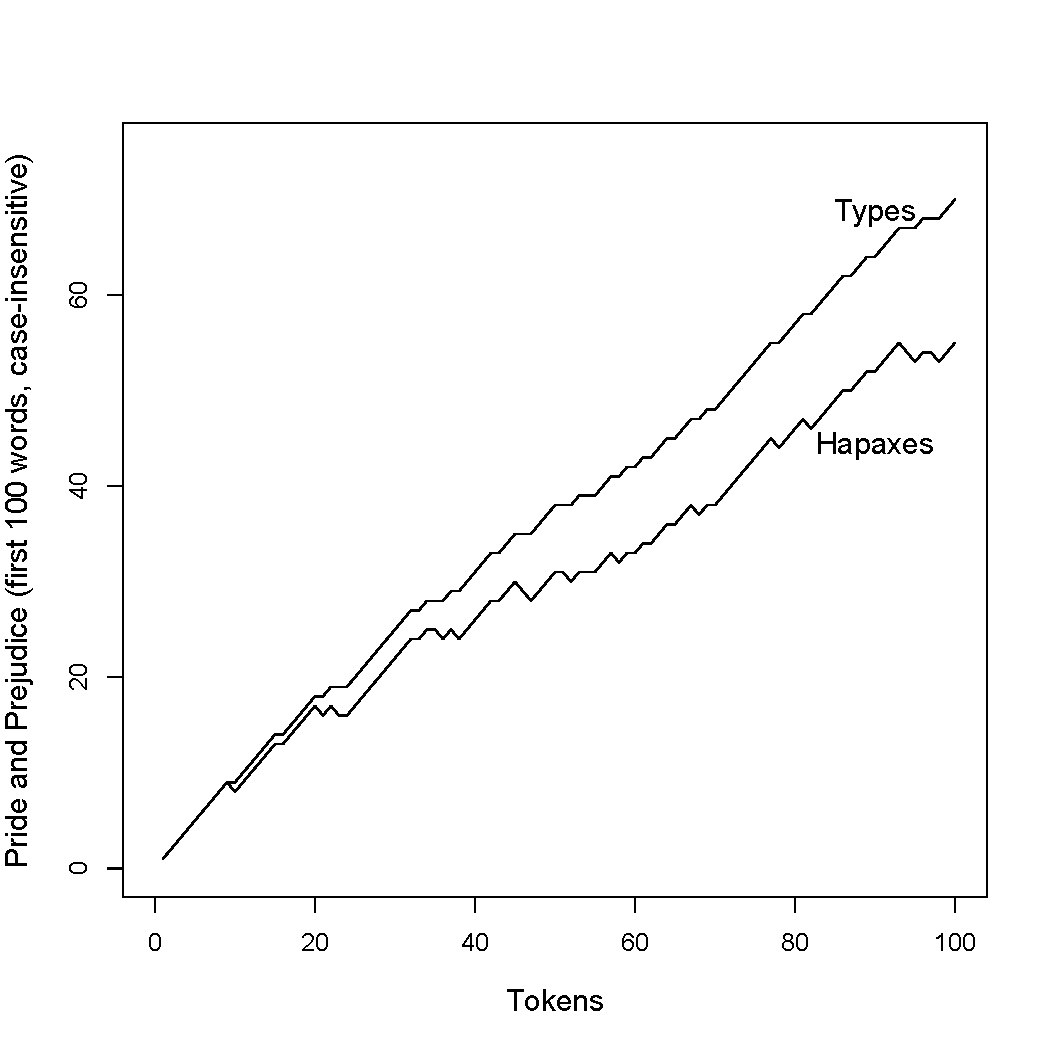
\includegraphics[width=\textwidth]{figures/prideandprejudiceonehundred}
\end{minipage}%
\begin{minipage}{.5\textwidth}
 \centering
 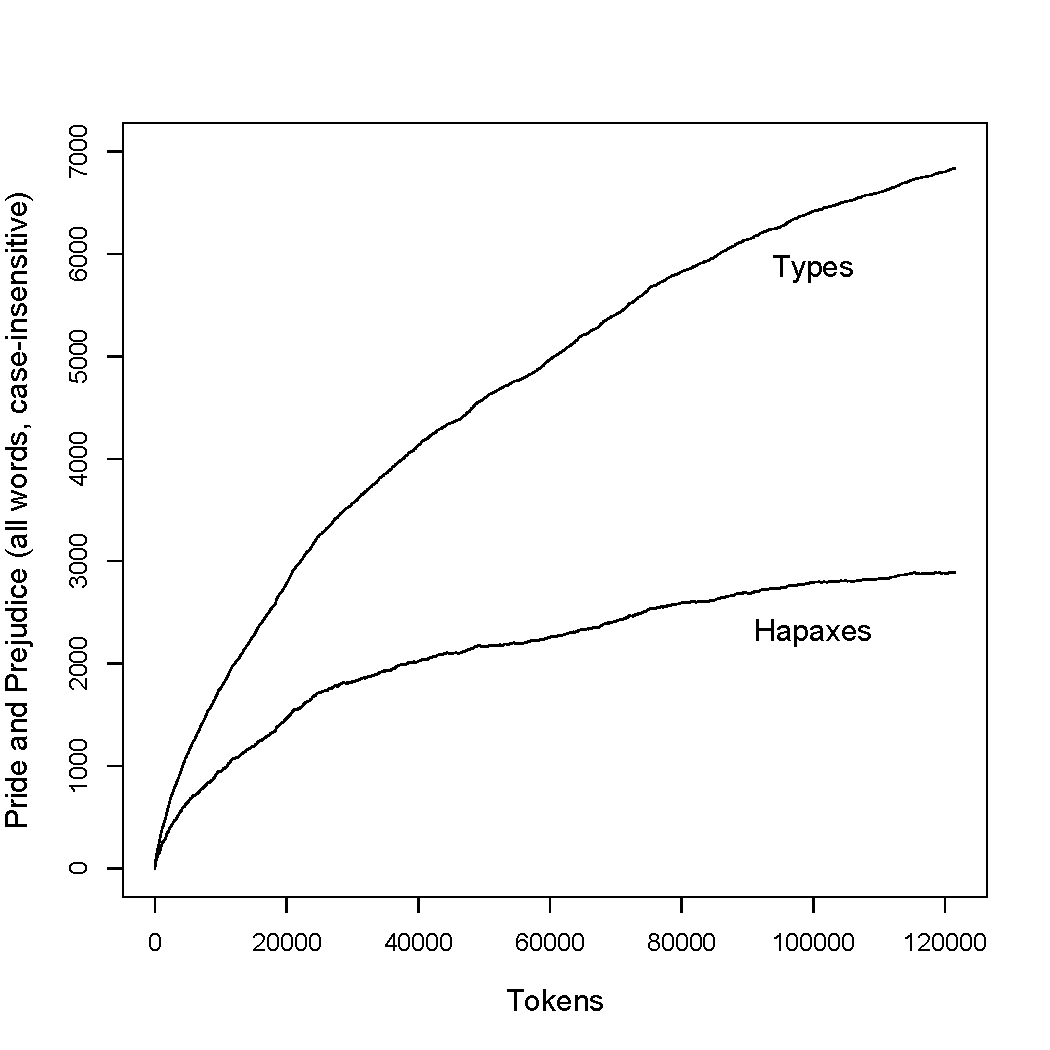
\includegraphics[width=\textwidth]{figures/prideandprejudiceall}
\end{minipage}
\end{figure}

As we can see by looking at the first 100 words, type \is{type (category)} and hapax \is{hapax legomenon} counts fall below the token counts fairly quickly: after 20 tokens, the TTR \is{type-token ratio} is $\nicefrac{18}{20} = 0.9$ and the HTR \is{hapax-token ratio} is $\nicefrac{17}{20} = 0.85$, after 40 tokens the TTR is $\nicefrac{31}{40} = 0.775$ and the HTR is $\nicefrac{26}{40} = 0.65$, after 60 tokens the HTR is $\nicefrac{42}{60} = 0.7$ and the TTR is $\nicefrac{33}{60} = 0.55$, and so on (note also how the hapax\hyp{}token \is{hapax legomenon} ratio sometimes drops before it rises again, as words that were hapaxes up to a particular point in the text reoccur and cease to be counted as hapaxes). If we zoom out and look at the entire novel, \is{literary language} we see that the growth in hapaxes slows considerably, to the extent that it has almost stopped by the time we reach the end of the novel. The growth in types \is{type (category)} also slows, although not as much as in the case of the hapaxes. \is{hapax legomenon} In both cases this means that the ratios will continue to fall as the number of tokens increases.

Now imagine we wanted to use the TTR \is{type-token ratio} and the HTR \is{hapax-token ratio} as measures of Jane Austen's overall lexical productivity \is{productivity} (referred to as ``lexical richness'' in computational stylistics \is{style} and in second\hyp{}language teaching): if we chose a small sample of her writing, the TTR and the HTR would be larger than if we chose a large \is{corpus size} sample, to the extent that the scores derived from the two samples would differ significantly. Table \ref{tab:austenttr} shows what would happen if we compared the TTR of the first chapter with the TTR of the entire rest of the novel. \is{literary language}

\begin{table}[!htbp]
\caption{Type/token ratios in the novel \textit{Pride and Prejudice}}
\label{tab:austenttr}
\begin{tabular}[t]{llccr}
\lsptoprule
 & & \multicolumn{2}{c}{\textvv{Type}} & \\
 & & \textvv{new} & \textvv{$\neg$new} & Total \\
\midrule
\textvv{\makecell[lt]{Text Sample}}
	& \textvv{first chapter}
		& \makecell[t]{\num{321}\\\small{(\num{47.29})}}
		& \makecell[t]{\num{6829}\\\small{(\num{7102.71})}}
		& \makecell[t]{\num{7150}\\} \\
	& \textvv{$\neg$first chapter}
		& \makecell[t]{\num{528}\\\small{(\num{801.71})}}
		& \makecell[t]{\num{120679}\\\small{(\num{120405.29})}}
		& \makecell[t]{\num{121207}\\} \\
\midrule
	& Total
		& \makecell[t]{\num{849}}
		& \makecell[t]{\num{127508}}
		& \makecell[t]{\num{128357}} \\
\lspbottomrule
\end{tabular}
\end{table}
% me: chisq.test(matrix(c(321,528,6829,120679),ncol=2),corr=FALSE)

The TTR \is{type-token ratio} for the first chapter is an impressive 0.3781, that for the rest of the novel \is{literary language} is a measly 0.0566, and the difference is highly significant ($\chi^2$ = 1688.7, df = 1, p < 0.001, $\phi$ = 0.1147). \is{chi-square test} But this is not because there is anything special about the first chapter; the TTR for the second chapter is 0.3910, that for the third is 0.3457, that for chapter 4 is 0.3943, and so on. The reason why the first chapter (or any chapter) looks as though it has a significantly higher TTR than the novel \is{literary language} as a whole is simply because the TTR will drop as the size \is{corpus size} of the text increases.

Therefore, comparing TTRs \is{type-token ratio} derived from samples of different sizes \is{corpus size} will always make the smaller sample look more productive. \is{productivity} In other words, we cannot compare such TTRs, let alone evaluate the differences statistically -- the result will simply be meaningless. The same is true for HTRs, \is{hapax-token ratio} with the added problem that, under certain circumstances, it will decrease at some point as we keep increasing the sample size: \is{corpus size} at some point, all possible words will have been used, so unless new words are added to the language, the number of hapaxes \is{hapax legomenon} will shrink again and finally drop to zero when all existing types \is{type (category)} have been used at least twice.

We will encounter the same problem when we compare the TTR \is{type-token ratio} or HTR \is{hapax-token ratio} of particular affixes \is{affix} or other linguistic phenomena, rather than that of a text. Consider Figures \ref{fig:izettrhtr}a and \ref{fig:izettrhtr}b, which show the TTR and the HTR of the verb \is{verb} suffixes \is{affix} \textit{-ise/-ize} (occurring in words like \textit{realize}, \textit{maximize} or \textit{liquidize}) and \textit{-ify} (occurring in words like \textit{identify}, \textit{intensify} or \textit{liquify}).

\begin{figure}
\caption{TTRs and HTRs for \textit{-ise/-ize} and \textit{-ify} in the LOB corpus}
\label{fig:izettrhtr}
\begin{minipage}{.5\textwidth}
 \centering
 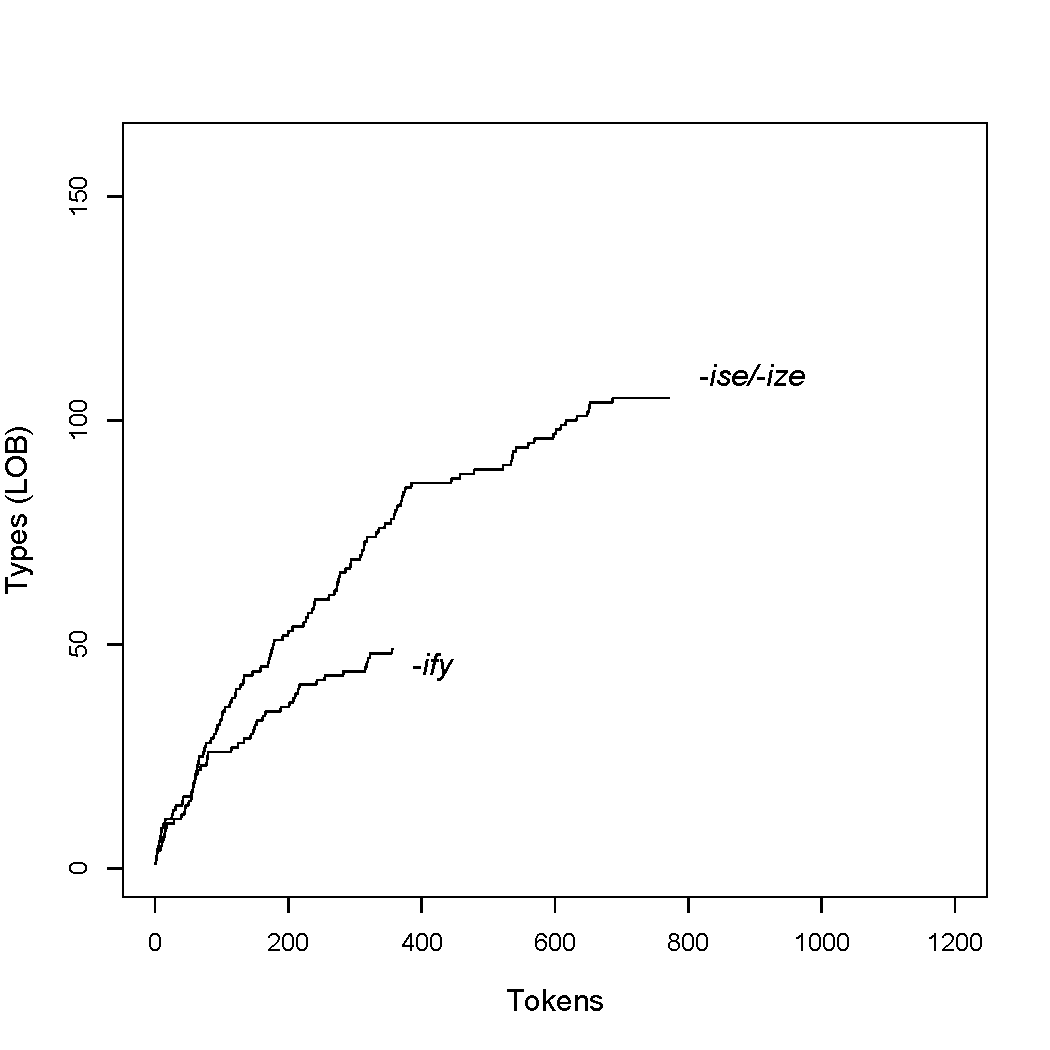
\includegraphics[width=\textwidth]{figures/lobiseifytypes}
\end{minipage}%
\begin{minipage}{.5\textwidth}
 \centering
 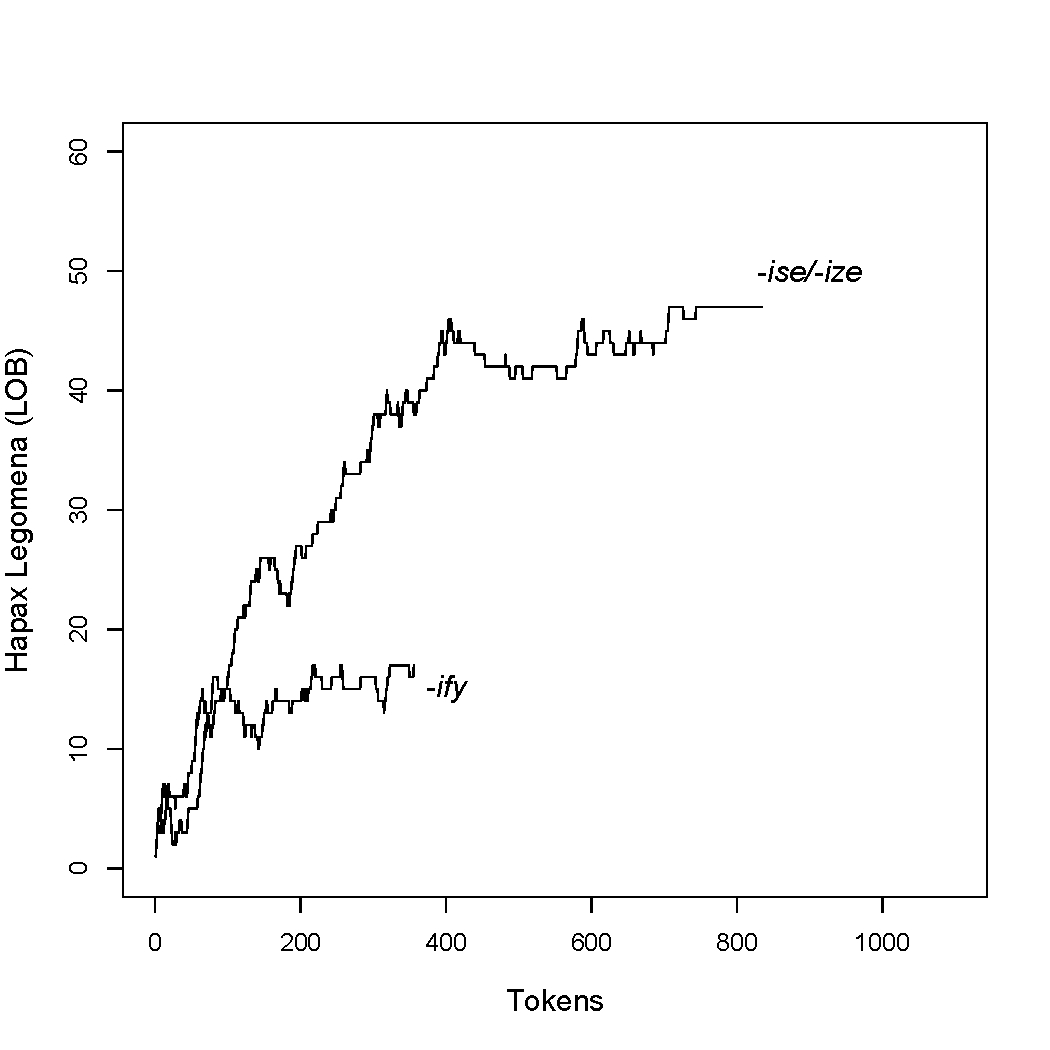
\includegraphics[width=\textwidth]{figures/lobiseifyhapaxes}
\end{minipage}
\end{figure}

As we can see, the TTR \is{type-token ratio} and HTR \is{hapax-token ratio} of both affixes \is{affix} behave roughly like that of Jane Austen's vocabulary as a whole as we increase sample size: \is{corpus size} both of them grow fairly quickly at first before their growth slows down; the latter happens more quickly in the case of the HTR than in the case of the TTR, and, again, we observe that the HTR sometimes decreases as types \is{type (category)} that were hapaxes \is{hapax legomenon} up to a particular point in the sample reoccur and cease to be hapaxes.

Taking into account the entire sample, the TTR \is{type-token ratio} for \textit{-ise/-ize} is $\nicefrac{105}{834} = 0.1259$ and that for \textit{-ify} is $\nicefrac{49}{356} = 0.1376$; it seems that \textit{-ise/-ize} is slightly more important to the lexicon \is{lexicon} of English than \textit{-ify}. A $\chi^2$ \is{chi-square test} test suggests that the difference is not significant (cf. Table \ref{tab:izeifyttr}; $\chi^2$ = 0.3053, df = 1, p > 0.05).

\begin{table}[!htbp]
\caption{Type/token ratios of \textit{-ise/-ize} and \textit{-ify} (LOB)}
\label{tab:izeifyttr}
\begin{tabular}[t]{llccr}
\lsptoprule
 & & \multicolumn{2}{c}{\textvv{Type}} & \\
 & & \textvv{new} & \textvv{seen before} & Total \\
\midrule
\textvv{\makecell[lt]{Affix}}
	& \textvv{-ise/-ize}
		& \makecell[t]{\num{105}\\\small{(\num{107.93})}}
		& \makecell[t]{\num{729}\\\small{(\num{726.07})}}
		& \makecell[t]{\num{834}\\} \\
	& \textvv{-ify}
		& \makecell[t]{\num{49}\\\small{(\num{46.07})}}
		& \makecell[t]{\num{307}\\\small{(\num{309.93})}}
		& \makecell[t]{\num{356}\\} \\
\midrule
	& Total
		& \makecell[t]{\num{154}}
		& \makecell[t]{\num{1036}}
		& \makecell[t]{\num{1190}} \\
\lspbottomrule
\multicolumn{5}{l}{\scriptsize{Supplementary Online Material: EWTN}} \\ %OSM
\end{tabular}
\end{table}
% me: chisq.test(matrix(c(105,49,729,307),ncol=2),corr=FALSE)

Likewise, taking into account the entire sample, the HTR \is{hapax-token ratio} for \textit{-ise/-ize} is $\nicefrac{47}{834} = 0.0563$ and that for \textit{-ify} is $\nicefrac{17}{365} = 0.0477$; it seems that \textit{-ise/-ize} is slightly more productive \is{productivity} than \textit{-ify}. However, again, the difference is not significant (cf. Table \ref{tab:izeifyhtr}; $\chi^2$ = 0.3628, df = 1, p > 0.05).

\begin{table}[!htbp]
\caption{Hapax/token ratios of \textit{-ise/-ize} and \textit{-ify} (LOB)}
\label{tab:izeifyhtr}
\begin{tabular}[t]{llccr}
\lsptoprule
 & & \multicolumn{2}{c}{\textvv{Type}} & \\
 & & \textvv{hapax} & \textvv{$\neg$hapax} & Total \\
\midrule
\textvv{\makecell[lt]{Affix}}
	& \textvv{-ise/-ize}
		& \makecell[t]{\num{47}\\\small{(\num{44.85})}}
		& \makecell[t]{\num{787}\\\small{(\num{789.15})}}
		& \makecell[t]{\num{834}\\} \\
	& \textvv{-ify}
		& \makecell[t]{\num{17}\\\small{(\num{19.15})}}
		& \makecell[t]{\num{339}\\\small{(\num{336.85})}}
		& \makecell[t]{\num{356}\\} \\
\midrule
	& Total
		& \makecell[t]{\num{64}}
		& \makecell[t]{\num{1126}}
		& \makecell[t]{\num{1190}} \\
\lspbottomrule
\end{tabular}
\end{table}
% me: chisq.test(matrix(c(47,17,787,339),ncol=2),corr=FALSE)

However, note that \textit{-ify} has a token \is{token (instance)} frequency \is{frequency, token} that is less than half of that of \textit{-ise/-ize}, so the sample is much smaller: as in the example of lexical richness in \textit{Pride and Prejudice}, this means that the TTR \is{type-token ratio} and the HTR \is{hapax-token ratio} of this smaller sample are exaggerated and our comparisons in Table \ref{tab:izeifyttr} and Table \ref{tab:izeifyhtr} as well as the accompanying statistics are, in fact, completely meaningless.

The simplest way of solving the problem of different sample sizes \is{corpus size} is to create samples of equal size for the purposes of comparison. We simply take the size of the smaller of our two samples and draw a random sample of the same size from the larger of the two samples (if our data sets are large enough, it would be even better to draw random samples for both affixes). \is{affix} This means that we lose some data, but there is nothing we can do about this (note that we can still include the discarded data in a qualitative \is{qualitative research} description \is{description} of the affix \is{affix} in question).\footnote{In studies of lexical richness, a measure called \textit{Mean Segmental Type\hyp{}Token Ratio} (MSTTR) \is{type-token ratio, mean segmental} is sometimes used \citep[cf.][]{johnson_program_1944}. This measure is derived by dividing the texts under investigation into segments of equal size (often segments of 100 words), determining the TTR \is{type-token ratio} for each segment, and then calculating an average TTR. This allows us to compare the TTR of texts of different sizes without discarding any data. However, this method is not applicable to the investigation of morphological \is{morphology} productivity, \is{productivity} as most samples of 100 words (or even 1000 or \num{10000} words) will typically not contain enough cases of a given morpheme to determine a meaningful TTR.}

Figures \ref{fig:izesamplettrhtr}a and \ref{fig:izesamplettrhtr}b show the growth rates of the TTR \is{type-token ratio} and the HTR \is{hapax-token ratio} of a sub\hyp{}sample of 356 tokens of \textit{-ise/-ize} in comparison with the total sample of the same size for \textit{-ify} (the sample was derived by first deleting every second hit, \is{hit} then every seventh hit and finally every ninetieth hit, making sure that the remaining hits are spread throughout the corpus).

\begin{figure}
\caption{TTRs and HTRs for \textit{-ise/-ize} and \textit{-ify} in the LOB corpus}
\label{fig:izesamplettrhtr}
\begin{minipage}{.5\textwidth}
 \centering
 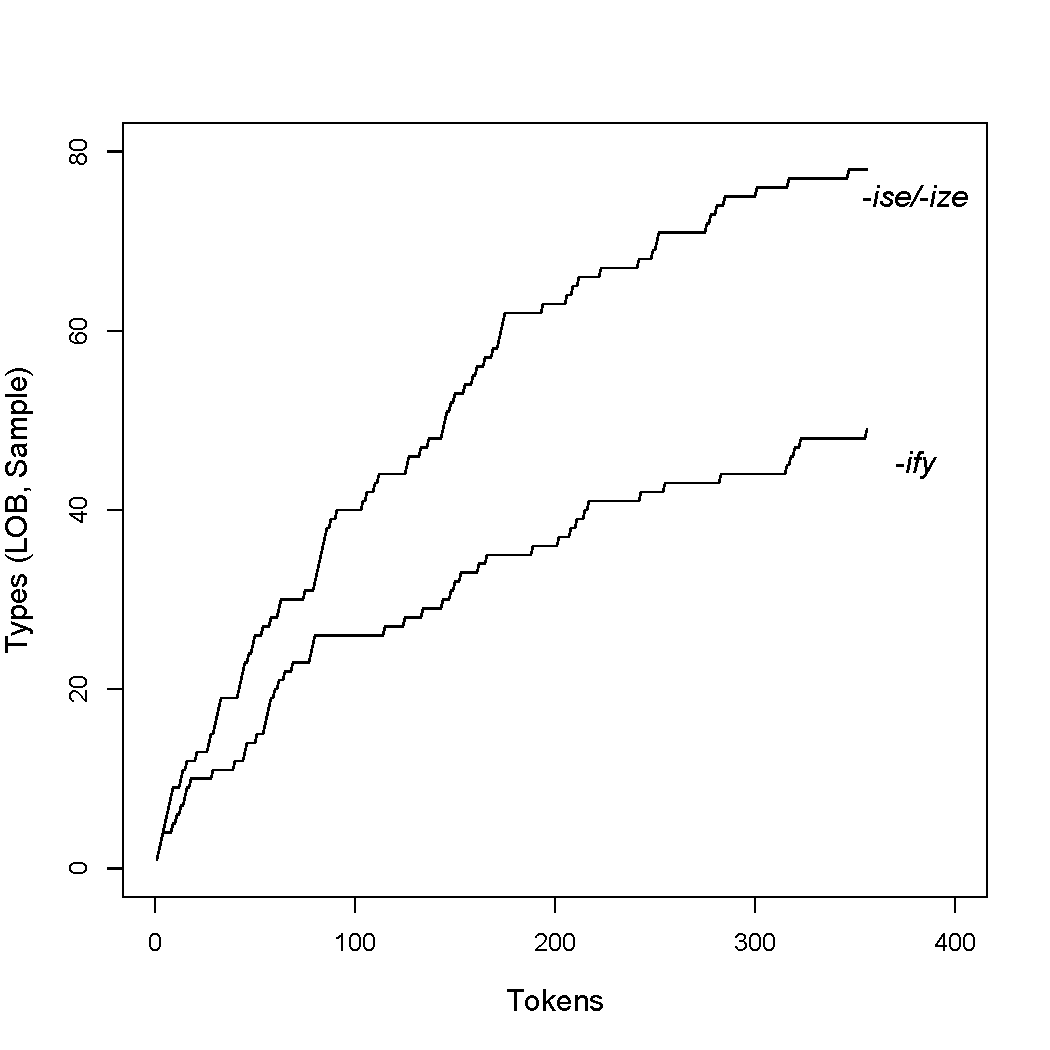
\includegraphics[width=\textwidth]{figures/lobsampleiseifytypes}
\end{minipage}
%
\begin{minipage}{.5\textwidth}
 \centering
 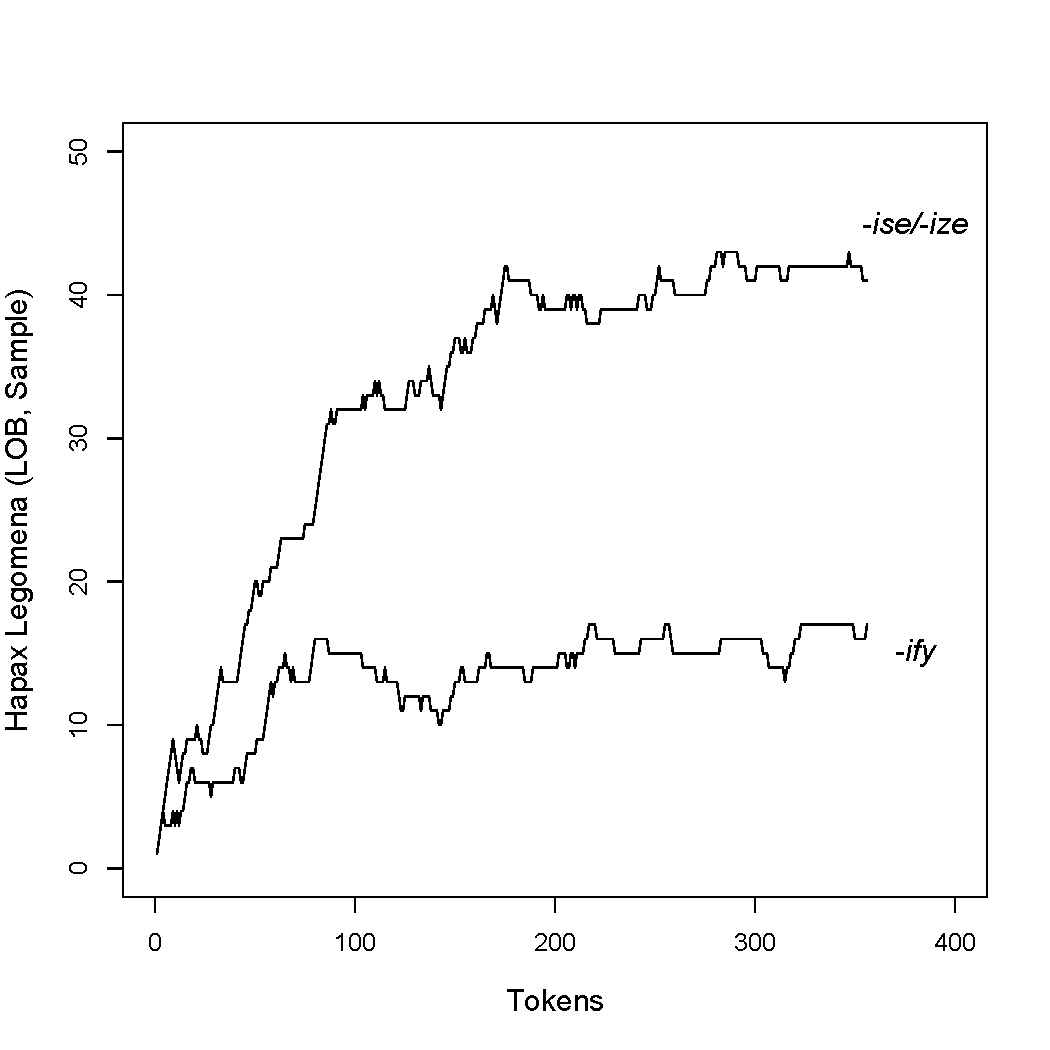
\includegraphics[width=\textwidth]{figures/lobsampleiseifyhapaxes}
\end{minipage}
\end{figure}

The TTR \is{type-token ratio} of \textit{-ise/-ize} based on the random sub\hyp{}sample is $\nicefrac{78}{356} = 0.2191$, that of \textit{-ify} is still $\nicefrac{49}{356} = 0.1376$; the difference between the two suffixes \is{affix} is much clearer now, and a $\chi^2$ test shows that it is very significant, although the effect size \is{effect size} is weak (cf. Table \ref{tab:izeifyttrsample}; $\chi^2$ = 8.06, df = 1, p < 0.01, $\phi$ = 0.1064).

\begin{table}[!htbp]
\caption{Type/token ratios of \textit{-ise/-ize}/\textit{-ise/-ize} (sample) and \textit{-ify} (LOB)}
\label{tab:izeifyttrsample}
\begin{tabular}[t]{llccr}
\lsptoprule
 & & \multicolumn{2}{c}{\textvv{Type}} & \\
 & & \textvv{new} & \textvv{seen before} & Total \\
\midrule
\textvv{\makecell[lt]{Affix}}
	& \textvv{-ise/-ize}
		& \makecell[t]{\num{78}\\\small{(\num{63.50})}}
		& \makecell[t]{\num{278}\\\small{(\num{292.50})}}
		& \makecell[t]{\num{356}\\} \\
	& \textvv{-ify}
		& \makecell[t]{\num{49}\\\small{(\num{63.50})}}
		& \makecell[t]{\num{307}\\\small{(\num{292.50})}}
		& \makecell[t]{\num{356}\\} \\
\midrule
	& Total
		& \makecell[t]{\num{127}}
		& \makecell[t]{\num{585}}
		& \makecell[t]{\num{712}} \\
\lspbottomrule
\end{tabular}
\end{table}
% me: chisq.test(matrix(c(78,49,278,307),ncol=2),corr=FALSE)

Likewise, the HTR \is{hapax-token ratio} of \textit{-ise/-ize} based on our sub\hyp{}sample is $\nicefrac{41}{356} = 0.1152$, the HTR of \textit{-ify} remains $\nicefrac{17}{365} = 0.0477$. Again, the difference is much clearer, and it, too, is now very significant, again with a weak effect size \is{effect size} (cf. Table \ref{tab:izeifyhtrsample}; $\chi^2$ = 10.81, df = 1, p < 0.01, $\phi$ = 0.1232). \is{chi-square test}

\begin{table}[!htbp]
\caption{Hapax/token ratios of \textit{-ise/-ize} (sample) and \textit{-ify} (LOB)}
\label{tab:izeifyhtrsample}
\begin{tabular}[t]{llccr}
\lsptoprule
 & & \multicolumn{2}{c}{\textvv{Type}} & \\
 & & \textvv{hapax} & \textvv{$\neg$hapax} & Total \\
\midrule
\textvv{\makecell[lt]{Affix}}
	& \textvv{-ise/-ize}
		& \makecell[t]{\num{41}\\\small{(\num{29.00})}}
		& \makecell[t]{\num{315}\\\small{(\num{327.00})}}
		& \makecell[t]{\num{356}\\} \\
	& \textvv{-ify}
		& \makecell[t]{\num{17}\\\small{(\num{29.00})}}
		& \makecell[t]{\num{339}\\\small{(\num{327.00})}}
		& \makecell[t]{\num{356}\\} \\
\midrule
	& Total
		& \makecell[t]{\num{58}}
		& \makecell[t]{\num{654}}
		& \makecell[t]{\num{712}} \\
\lspbottomrule
\end{tabular}
\end{table}
% me: chisq.test(matrix(c(41,17,315,339),ncol=2),corr=FALSE)

In the case of the HTR, \is{hapax-token ratio} decreasing the sample size \is{corpus size} is slightly more problematic than in the case of the TTR. \is{type-token ratio} The proportion of hapax \is{hapax legomenon} legomena actually resulting from productive \is{productivity} rule application becomes smaller as sample size decreases. Take example (\ref{ex:shakspearecinna}) from Shakespeare's \textit{Julius Caesar} above: the words \textit{directly}, \textit{briefly} and \textit{truly} are all hapaxes \is{hapax legomenon} in the passage cited, but they are clearly not the result of a productively \is{productivity} applied rule\hyp{}application (all of them have their own entries in the OALD, for example). As we increase the sample, they cease to be hapaxes (\textit{directly} occurs 9 times in the entire play, \textit{briefly} occurs 4 times and \textit{truly} 8 times). This means that while we must draw random samples of equal size \is{corpus size} in order to compare HTRs, \is{hapax-token ratio} we should make sure that these samples are as large as possible.

\section{Case studies}
\label{sec:moprphologycasestudies}

\subsection{Morphemes and stems}
\label{sec:morphemesandstems}

One general question in (derivational) morphology \is{morphology} concerns the category of the stem \is{statistics} which an affix \is{affix} may be attached to. This is obviously a descriptive \is{description} issue that can be investigated on the basis of corpora very straightforwardly simply by identifying all types \is{type (category)} containing the affix \is{affix} in question and describing their internal structure. In the case of affixes \is{affix} with low productivity, \is{productivity} this will typically add little insight over studies based on dictionaries, \is{dictionary} but for productive affixes, \is{affix} a corpus analysis will yield more detailed and comprehensive results since corpora will contain spontaneously produced or at least recently created items not (yet) found in dictionaries. \is{dictionary} Such newly created words will often offer particularly clear insights into constraints that an affix \is{affix} places on its stems. \is{statistics} Finally, corpus\hyp{}based approaches are without an alternative in diachronic \is{diachrony} studies and yield particularly interesting results when used to study changes in the quality or degree of productivity, \is{productivity} (cf. for example \citealt{dalton-puffer_french_1996}).

In the study of constraints placed by derivational affixes \is{affix} on the stems \is{statistics} that they combine with, the combinability of derivational morphemes \is{morphology} (in an absolute sense or in terms of preferences) is of particular interest. Again, corpus linguistics is a uniquely useful tool to investigate this.

Finally, there are cases where two derivational morphemes \is{morphology} are in direct competition because they are functionally roughly equivalent (e.g. \textit{-ness} and \textit{-ity}, both of which form abstract nouns \is{noun} from typically adjectival \is{adjective} bases, \textit{-ise/-ize} and \textit{-ify}, which form process \is{aktionsart} verbs \is{verb} from nominal \is{noun} and adjectival \is{adjective} bases, or \textit{-ic} and \textit{-ical}, which form adjectives \is{adjective} from typically nominal bases). Here, too, corpus linguistics provides useful tools, for example to determine whether the choice between affixes \is{affix} is influenced by syntactic, \is{syntax} semantic or phonological properties of stems. \is{statistics}

\subsubsection{Case study: Phonological constraints on \textit{-ify}}
\label{sec:phonologicalconstraintsofify}

As part of a larger argument that \textit{-ise/-ize} and \textit{-ify} should be considered phonologically conditioned allomorphs, \citet{plag_morphological_1999} investigates the phonological constraints that \textit{-ify} places on its stems. \is{statistics} First, he summarizes the properties of stems in established words with \textit{-ify} as observed in the literature. Second, he checks these observations against a sample of twenty\hyp{}three recent (20th century) coinages from a corpus of neologisms \is{neologism} to ensure that the constraints also apply to productive \is{productivity} uses of the affix. \is{affix} This is a reasonable approach. The affix \is{affix} was first borrowed into English as part of a large number of French loanwords beginning in the late 13th century; two thirds of all non\hyp{}hapax \is{hapax legomenon} types \is{type (category)} and 19 of the 20 most frequent types found in the BNC \is{BNC} are older than the 19th century. Thus, it is possible that the constraints observed in the literature are historical remnants not relevant to new coinages.

The most obvious constraint is that the syllable \is{syllable} directly preceding \textit{-ify} must carry the main stress of the word. This has a number of consequences, of which we will focus on two: First, monosyllabic stems \is{statistics} (as in \textit{falsify}) are preferred, since they always meet this criterion. Second, if a polysyllabic stem ends in an unstressed syllable, the stress must be shifted to that syllable (as in \textit{perSONify} from \textit{PERson});\footnote{This is a simplification: stress\hyp{}shift only occurs with unstressed closed syllables or sequence of two unstressed syllables \is{syllable} (\textit{SYLlable} -- \textit{sylLAbify}). Occasionally, stem\hyp{}final \is{statistics} consonants \is{consonant} are deleted (as in \textit{liquid} -- \textit{liquify}); cf. \citet{plag_morphological_1999} for a more detailed discussion.} since this reduces the transparency of the stem, there should be a preference for those polysyllabic stems \is{statistics} which already have the stress on the final syllable. \is{syllable}

Plag simply checks his neologisms \is{neologism} against the literature, but we will evaluate the claims from the literature quantitatively. \is{quantitative research} Our main hypothesis will be that neologisms with \textit{-ify} do not differ from established types \is{type (category)} with respect to the fact that the syllable \is{syllable} directly preceding the suffix \is{affix} must carry primary stress, with the consequences that (i) they prefer monosyllabic stems, \is{statistics} and (ii) if the stem \is{statistics} is polysyllabic, they prefer stems that already have the primary stress on the last syllable. Our independent variable is therefore \textsc{Lexical Status} with the values \textsc{established word} vs. \textsc{neologism} \is{neologism} (which will be operationalized \is{operationalization} presently). Our dependent variables are \textsc{Syllabicity} \is{syllable} with the values \textsc{monosyllabic} and \textsc{polysyllabic}, and \textsc{Stress Shift} with the values \textsc{required} vs. \textsc{not required} (both of which should be self\hyp{}explanatory).

Our design \is{research design} compares two predefined groups of types \is{type (category)} with respect to the distribution \is{distribution, conditional} that particular properties have in these groups; this means that we do not need to calculate TTRs \is{type-token ratio} or HTRs, \is{hapax-token ratio} but that we need operational \is{operationalization} definitions of the values \textsc{established word} and \textsc{neologism}. \is{neologism} Following Plag, let us define \textsc{neologism} as ``coined in the 20th century'', but let us use a large historical dictionary \is{dictionary} (the Oxford English Dictionary, \is{OED} 3rd edition) and a large \is{corpus size} corpus (the BNC) \is{BNC} in order to identify words matching this definition; this will give us the opportunity to evaluate the idea that hapax \is{hapax legomenon} legomena are a good way of operationalizing productivity. \is{productivity}

Excluding cases with prefixed \is{affix} stems, \is{statistics} the OED \is{OED} contains 456 entries or sub\hyp{}entries for verbs \is{verb} with \textit{-ify}, 31 of which are first documented in the 20th century. Of the latter, 21 do not occur in the BNC \is{BNC} at all, and 10 do occur in the BNC, but are not hapaxes \is{hapax legomenon} (see Table \ref{tab:ifyneologisms} below). The BNC contains 30 hapaxes, of which 13 are spelling errors and 7 are first documented in the OED \is{OED} before the 20th century (\textit{carbonify}, \textit{churchify}, \textit{hornify}, \textit{preachify}, \textit{saponify}, \textit{solemnify}, \textit{townify}). This leaves 10 hapaxes that are plausibly regarded as neologisms, \is{neologism} none of which are listed in the OED \is{OED} (again, see Table \ref{tab:ifyneologisms}). In addition, there are four types \is{type (category)} in the BNC \is{BNC} that are not hapax \is{hapax legomenon} legomena, but that are not listed in the OED; \is{OED} careful cross\hyp{}checks show that these are also neologisms. Combining all sources, this gives us 45 neologisms.

\begin{table}[!htbp]
\caption{Twentieth century neologisms with \textit{-ify}}
\label{tab:ifyneologisms}
\begin{tabular}[t]{ll}
\lsptoprule
\multicolumn{2}{l}{First documented in the OED in the 20th century} \\
(i) & also occur in the BNC, but not as hapaxes: \\
 & \makecell[tl]{\textit{bourgeoisify}, \textit{esterify}, \textit{gentrify}, \textit{karstify}, \textit{massify}, \textit{Nazify}, \textit{syllabify}, \\ \textit{vinify}, \textit{yuppify}, \textit{zombify}} \\
(ii) & do not occur in the BNC: \\
 & \makecell[tl]{\textit{ammonify}, \textit{aridify}, \textit{electronify}, \textit{glassify}, \textit{humify}, \textit{iconify}, \textit{jazzify}, \\ \textit{mattify}, \textit{metrify}, \textit{mucify}, \textit{nannify}, \textit{passivify}, \textit{plastify}, \textit{probabilify}, \\\textit{Prussify}, \textit{rancidify}, \textit{sinify}, \textit{trendify}, \textit{trustify}, \textit{tubify}, \textit{youthify}} \\
\multicolumn{2}{l}{Not documented in the OED at all} \\
(iii) & occur in the BNC as hapaxes: \\
 & \makecell[tl]{\textit{faintify}, \textit{fuzzify}, \textit{lewisify}, \textit{rawify}, \textit{rockify}, \textit{sickify}, \textit{sonify}, \textit{validify}, \\ \textit{yankify}, \textit{yukkify}} \\
(iv) & occur in the BNC, but not as hapaxes: \\
 & \makecell[tl]{\textit{commodify}, \textit{desertify}, \textit{extensify}, \textit{geriatrify}} \\
\lspbottomrule
\end{tabular}
\end{table}

Before we turn to the definition and sampling of established types, \is{type (category)} let us determine the precision \is{precision} and recall \is{recall} of the operational \is{operationalization} definition of neologism \is{neologism} as ``hapax \is{hapax legomenon} legomenon'' in the BNC, \is{BNC} using the formulas introduced in Chapter \ref{ch:retrievalannotation}. Precision is defined as the number of true positives (items that were found and that actually are what they are supposed to be) divided by the number of all positives (all items found); 10 of the 30 hapaxes in the BNC \is{BNC} are actually neologisms, so the precision is $\nicefrac{10}{30} = 0.3333$. Recall is defined as the number of true positives divided by the number of true positives and false negatives (i.e. all items that should have been found); 10 of the 45 neologisms \is{neologism} were actually found by using the hapax definition, so the recall is $\nicefrac{10}{45} = 0.2222$. In other words, neither precision \is{precision} nor recall of the method are very good, at least for moderately productive \is{productivity} affixes \is{affix} like \textit{-ify} (the method will presumably give better results with highly productive affixes). \is{affix} Let us also determine the recall of neologisms from the OED \is{OED} (using the definition ``first documented in the 20th century according to the OED''): the OED \is{OED} lists 31 of the 45 neologisms, \is{neologism} so the recall is $\nicefrac{31}{45} = 0.6889$; this is much better than the recall \is{recall} of the corpus\hyp{}based hapax \is{hapax legomenon} definition, but it also shows that if we combine corpus data and dictionary \is{dictionary} data, we can increase coverage substantially even for moderately productive \is{productivity} affixes. \is{affix}

Let us now turn to the definition of \textsc{established types}. \is{type (category)} Given our definition of \textsc{neologisms}, \is{neologism} established types would first have to be documented before the 20th century, so we could use the 420 types in the OED \is{OED} that meet this criterion (again, excluding prefixed \is{affix} forms). However, these 420 types contain many very rare or even obsolete forms, like \textit{duplify} ``to make double'', \textit{eaglify} ``to make into an eagle'' or \textit{naucify} ``to hold in low esteem''. Clearly, these are not ``established'' in any meaningful sense, so let us add the requirement that a type must occur in the BNC \is{BNC} at least twice to count as established. Let us further limit the category to verbs \is{verb} first documented before the 19th century, in order to leave a clear diachronic \is{diachrony} gap between the established types \is{type (category)} and the productive \is{productivity} types. This leaves the words in Table \ref{tab:ifycontrol}.\footnote{Interestingly, leaving out words coined in the 19th century does not make much of a difference: although the 19th century saw a large number of coinages (with 138 new types \is{type (category)} it was the most productive \is{productivity} century in the history of the suffix), \is{affix} few of these are frequent enough today to occur in the BNC; \is{BNC} if anything, we should actually extend our definition of neologisms \is{neologism} to include the 19th century.}

\begin{table}[!htbp]
\caption{Control sample of established types with the suffix \textit{-ify}.}
\label{tab:ifycontrol}
\begin{tabular}[t]{l}
\lsptoprule
\makecell[tl]{
\textit{acidify}, \textit{amplify}, \textit{beatify}, \textit{beautify}, \textit{certify}, \textit{clarify}, \textit{classify}, \\ \textit{crucify}, \textit{damnify}, \textit{deify}, \textit{dignify}, \textit{diversify}, \textit{edify}, \textit{electrify}, \\ \textit{exemplify}, \textit{falsify}, \textit{fortify}, \textit{Frenchify}, \textit{fructify}, \textit{glorify}, \textit{gratify}, \\ \textit{identify}, \textit{indemnify}, \textit{justify}, \textit{liquify}\slash \textit{liquefy}, \textit{magnify}, \textit{modify}, \\ \textit{mollify}, \textit{mortify}, \textit{mummify}, \textit{notify}, \textit{nullify}, \textit{ossify}, \textit{pacify}, \\ \textit{personify}, \textit{petrify}, \textit{prettify}, \textit{purify}, \textit{qualify}, \textit{quantify}, \textit{ramify}, \\ \textit{rarify}, \textit{ratify}, \textit{rectify}, \textit{sacrify}, \textit{sanctify}, \textit{satisfy}, \textit{scarify}, \\ \textit{signify}, \textit{simplify}, \textit{solidify}, \textit{specify}, \textit{stratify}, \textit{stultify}, \textit{terrify}, \\ \textit{testify}, \textit{transmogrify}, \textit{typify}, \textit{uglify}, \textit{unify}, \textit{verify}, \textit{versify}, \\ \textit{vilify}, \textit{vitrify}, \textit{vivify}} \\
\lspbottomrule
\end{tabular}
\end{table}

Let us now evaluate the hypotheses. Table \ref{tab:ifysyllabicity} shows the type \is{type (category)} frequencies \is{frequency, type} for monosyllabic \is{syllable} and polysyllabic stems \is{statistics} in the two samples. In both cases, there is a preference for monosyllabic stems (as expected), \is{frequency, expected} but interestingly, this preference is less strong among the neologisms \is{neologism} than among the established types and this difference is very significant ($\chi^2 = 7.37, df = 1, p < 0.01 , \phi = 0.2577$). \is{chi-square test}

\begin{table}[!htbp]
\caption{Monosyllabic and bisyllabic stems with \textit{-ify}}
\label{tab:ifysyllabicity}
\begin{tabular}[t]{llccr}
\lsptoprule
 & & \multicolumn{2}{c}{\textvv{Number of Syllables}} & \\
 & & \textvv{monosyllabic} & \textvv{polysyllabic} & Total \\
\midrule
\textvv{\makecell[lt]{Status}}
	& \textvv{established}
		& \makecell[t]{\num{57}\\\small{(\num{51.14})}}
		& \makecell[t]{\num{9}\\\small{(\num{14.86})}}
		& \makecell[t]{\num{66}\\} \\
	& \textvv{neologism}
		& \makecell[t]{\num{29}\\\small{(\num{34.86})}}
		& \makecell[t]{\num{16}\\\small{(\num{10.14})}}
		& \makecell[t]{\num{45}\\} \\
\midrule
	& Total
		& \makecell[t]{\num{86}}
		& \makecell[t]{\num{25}}
		& \makecell[t]{\num{111}} \\
\lspbottomrule
\end{tabular}
\end{table}
% me: chisq.test(matrix(c(57,29,9,16),ncol=2),corr=FALSE)

Given the fact that there is a significantly higher number of neologisms \is{neologism} with polysyllabic \is{syllable} stems \is{statistics} than expected \is{frequency, expected} on the basis of established types, \is{type (category)} the second hypothesis becomes more interesting: does this higher number of polysyllabic \is{syllable} stems \is{statistics} correspond with a greater willingness to apply it to stems that then have to undergo stress shift (which would be contrary to our hypothesis, which assumes that there will be no difference between established types and neologisms)? \is{neologism}

Table \ref{tab:ifystressshift} shows the relevant data: it seems that there might indeed be such a greater willingness, as the number of neologisms \is{neologism} with polysyllabic \is{syllable} stems \is{statistics} requiring stress shift is higher than expected; \is{frequency, expected} however, the difference is not statistically significant ($\chi^2$ = 1.96, df = 1, p > 0.05, $\phi$ = 0.28) (strictly speaking, we cannot use the $\chi^2$ \is{chi-square test} test here, since half of the expected frequencies are below 5, but Fisher's exact test \is{Fisher's exact test} confirms that the difference is not significant).

\begin{table}[!htbp]
\caption{Stress shift with polysyllabic stems with \textit{-ify}}
\label{tab:ifystressshift}
\begin{tabular}[t]{llccr}
\lsptoprule
 & & \multicolumn{2}{c}{\textvv{Shift}} & \\
 & & \textvv{not required} & \textvv{required} & Total \\
\midrule
\textvv{\makecell[lt]{Status}}
	& \textvv{established}
		& \makecell[t]{\num{3}\\\small{(\num{4.68})}}
		& \makecell[t]{\num{6}\\\small{(\num{4.32})}}
		& \makecell[t]{\num{9}\\} \\
	& \textvv{neologism}
		& \makecell[t]{\num{10}\\\small{(\num{8.32})}}
		& \makecell[t]{\num{6}\\\small{(\num{7.68})}}
		& \makecell[t]{\num{16}\\} \\
\midrule
	& Total
		& \makecell[t]{\num{13}}
		& \makecell[t]{\num{12}}
		& \makecell[t]{\num{25}} \\
\lspbottomrule
\end{tabular}
\end{table}
% me: chisq.test(matrix(c(3,10,6,6),ncol=2),corr=FALSE)

This case study demonstrates some of the problems and advantages of using corpora to identify neologisms \is{neologism} in addition to existing dictionaries. \is{dictionary} It also constitutes an example of a purely type\hyp{}based \is{type (category)} research design; \is{research design} note, again, that such a design is possible here because we are not interested in the type frequency \is{frequency, type} of a particular affix \is{affix} under different conditions (in which case we would have to calculate a TTR \is{type-token ratio} to adjust for different sample sizes), \is{corpus size} but in the distribution \is{distribution, conditional} of the variables \textsc{Syllable Length} \is{syllable} \is{length} and \textsc{Stress Shift} in two qualitatively different categories of types. \is{type (category)} Finally, note that the study comes to different conclusions than the impressionistic analysis in \citet{plag_morphological_1999}, so it demonstrates the advantages of strictly quantified designs.

\subsubsection{Case study: Semantic differences between \textit{-ic} and \textit{-ical}}
\label{sec:semanticdifferencesbetweenicandical}

Affixes, like words, can be related to other affixes \is{affix} by lexical relations like synonymy, \is{synonymy} antonymy, \is{antonymy} etc. In the case of (roughly) synonymous affixes, \is{affix} an obvious research question is what determines the choice between them -- for example, whether there are more fine\hyp{}grained semantic \is{semantics} differences that are not immediately apparent.

One way of approaching this question is to focus on stems \is{statistics} that occur with both affixes \is{affix} (such as \textit{liqui(d)} in \textit{liquidize} and \textit{liquify}\slash \textit{liquefy}, \textit{scarce} in \textit{scarceness} and \textit{scarcity} or \textit{electr-} in \textit{electric} and \textit{electrical}) and to investigate the semantic \is{semantics} contexts in which they occur -- for example, by categorizing \is{categorization} their collocates, \is{collocation} analogous to the way \citet{taylor_near_2003} categorizes collocates of \textit{high} and \textit{tall} (cf. Chapter \ref{ch:collocation}, Section \ref{sec:nearsynonyms}).

A good example of this approach is found in \citet{kaunisto_electric/electrical_1999}, who investigates the pairs \textit{electric}\slash \textit{electrical} and \textit{classic}\slash \textit{classical} on the basis of the British Newspaper \is{newspaper language} \textit{Daily Telegraph}. Since his corpus is not accessible, let us use the LOB \is{LOB} corpus instead to replicate \is{replicability} his study for \textit{electric}\slash \textit{electrical}. It is a study with two nominal \is{nominal data} variables: \textsc{Affix Variant} (with the values \textsc{-ic} and \textsc{-ical}), and \textsc{Semantic Category} (with a set of values to be discussed presently). Note that this design \is{research design} can be based straightforwardly on token \is{token (instance)} frequency, \is{frequency, token} as we are not concerned with the relationship between the stem \is{statistics} and the affix, \is{affix} but with the relationship between the stem\hyp{}affix combination and the nouns \is{noun} modified by it. Put differently, we are not using the token \is{token (instance)} frequency of a stem\hyp{}affix combination, but of the collocates \is{collocation} of words derived by a particular affix. \is{affix}

Kaunisto uses a mixture of dictionaries \is{dictionary} and existing literature to identify potentially interesting values for the variable \textsc{Semantic Category}; we will restrict ourselves to dictionaries here. Consider the definitions from six major dictionaries \is{dictionary} in (\ref{ex:definitionelectric}) and (\ref{ex:definitionelectrical}):

\begin{exe}
\ex \textit{electric}
\begin{xlist}
\label{ex:definitionelectric}
\ex connected with electricity; using, produced by or producing electricity (OALD)
\ex of or relating to electricity; operated by electricity (MW)
\ex working by electricity; used for carrying electricity; relating to electricity (MD)
\ex of, produced by, or worked by electricity (CALD)
\ex needing electricity to work, produced by electricity, or used for carrying electricity (LDCE)
\ex work$[$ing$]$ by means of electricity; produced by electricity; designed to carry electricity; refer$[$ring$]$ to the supply of electricity (Cobuild)
\end{xlist}
\end{exe}

\begin{exe}
\ex \textit{electrical}
\begin{xlist}
\label{ex:definitionelectrical}
\ex connected with electricity; using or producing electricity (OALD)
\ex of or relating to electricity; operated by electricity (MW) $[$mentioned as a synonym under corresp. sense of \textit{electric}$]$
\ex working by electricity; relating to electricity (MD)
\ex related to electricity (CALD, LDCE)
\ex work[ing] by means of electricity; supply[ing] or us[ing] electricity; energy ... in the form of electricity; involved in the production and supply of electricity or electrical goods (Cobuild)
\end{xlist}
\end{exe}

MW treats the two words as largely synonymous \is{synonymy} and OALD distinguishes them only insofar as mentioning for \textit{electric}, but not \textit{electrical}, that it may refer to phenomena ``produced by electricity'' (this is meant to cover cases like \textit{electric current\slash charge}); however, since both words are also defined as referring to anything ``connected with electricity'', this is not much of a differentiation (the entry for \textit{electrical} also mentions \textit{electrical power\slash energy}). Macmillan's Dictionary \is{dictionary} also treats them as largely synonymous, \is{synonymy} although it is pointed out specifically that \textit{electric} refers to entities ``carrying electricity'' (citing \textit{electric outlet\slash plug\slash cord}). CALD and LDCE present \textit{electrical} as a more general word for anything ``related to electricity'', whereas they mention specifically that \textit{electric} is used for things ``worked by electricity'' (e.g. \textit{electric light\slash appliance}) or ``carrying electricity'' (presumably \textit{cords}, \textit{outlets}, etc.) and phenomena produced by electricity (presumably \textit{current}, \textit{charge}, etc.). Collins presents both words as referring to electric(al) appliances, with \textit{electric} additionally referring to things ``produced by electricity'', ``designed to carry electricity'' or being related to the ``supply of electricity'' and \textit{electrical} additionally referring to ``energy'' or entities ``involved in the production and supply of electricity'' (presumably energy companies, engineers, etc.).

Summarizing, we can posit the following four broad values for our variable \textsc{Semantic Category}, with definitions that are hopefully specific enough to serve as an annotation \is{annotation} scheme:

\begin{itemize}

\item \textsc{devices} and appliances working by electricity (\textit{light}, \textit{appliance}, etc.)

\item \textsc{energy} in the form of electricity (\textit{power}, \textit{current}, \textit{charge}, \textit{energy}, etc.)

\item the \textsc{industry} researching, producing or supplying energy, i.e. companies and the people working there (\textit{company}, \textit{engineer}, etc.)

\item \textsc{circuits}, broadly defined as entities producing or carrying electricity, including (\textit{cord}, \textit{outlet}, \textit{plug}, but also \textit{power plant}, etc.)

\end{itemize}

The definitions are too heterogeneous to base a specific hypothesis on them, but we might broadly expect \textit{electric} to be more typical for the categories \textvv{device} and \textvv{circuit} and \textit{electrical} for the category \textvv{industry}.

Table \ref{tab:electricalentitieslob} shows the token \is{token (instance)} frequency \is{frequency, token} with which nouns \is{noun} from these categories are referred to as \textit{electric} or \textit{electrical} in the LOB \is{LOB} corpus; in order to understand how these nouns were categorized, \is{categorization} it also lists all types \is{type (category)} found for each category (one example was discarded because it was metaphorical). \is{figurative language} \is{metaphor}

\begin{table}[!htbp]
\caption{Entities described as \textit{electric} or \textit{electrical} in the LOB corpus}
\label{tab:electricalentitieslob}
\resizebox{0.9\textwidth}{!}{%
\begin{tabular}[t]{lccr}
\lsptoprule
 & \multicolumn{2}{c}{\textvv{Adjective}} & \\
\textvv{Noun} & \textvv{electric} & \textvv{electrical} & Total \\
\midrule
\textvv{\makecell[tl]{device}}
	& \makecell[t]{\begin{tabular}[t]{lS[table-format=2.2]}
		\small{\textit{Obs.:}} & 17 \\
		\small{\textit{Exp.:}} & 12.077922 \\
		\small{\textit{$\chi^2$:}} & 2.005879 \\
		\multicolumn{2}{l}{
			\begin{minipage}[t]{0.3\textwidth} \raggedright
			\footnotesize{\textit{bulb}, \textit{calculating machine}, \textit{chair}, \textit{cooker}, \textit{dog}, \textit{drill}, \textit{fence}, \textit{fire}, \textit{heating element}, \textit{light switch}, \textit{motor}, \textit{mowing}, \textit{stove}, \textit{torch}, \textit{tricycle}}
			\end{minipage}}
		\end{tabular}}
	& \makecell[t]{\begin{tabular}[t]{lS[table-format=2.2]}
		\small{\textit{Obs.:}} & 13 \\
		\small{\textit{Exp.:}} & 17.922078 \\
		\small{\textit{$\chi^2$:}} & 1.351788 \\
		\multicolumn{2}{l}{
			\begin{minipage}[t]{0.3\textwidth} \raggedright
			\footnotesize{\textit{amplifier}, \textit{apparatus}, \textit{fire}, \textit{goods}, \textit{machine}, \textit{machinery}, \textit{power unit}, \textit{sign}, \textit{supply}, \textit{system}, \textit{system}, \textit{transmission}}
		\end{minipage}}
		\end{tabular}}
	& 30 \\[3.1cm]
\textvv{\makecell[tl]{energy}}
	& \makecell[t]{\begin{tabular}[t]{lS[table-format=2.2]}
		\small{\textit{Obs.:}} & 11 \\
		\small{\textit{Exp.:}} & 9.662338 \\
		\small{\textit{$\chi^2$:}} & 0.185187 \\
		\multicolumn{2}{l}{
			\begin{minipage}[t]{0.3\textwidth} \raggedright
			\footnotesize{\textit{attraction}, \textit{bill}, \textit{blue}, \textit{current}, \textit{effect}, \textit{field}, \textit{force}, \textit{light}, \textit{space constant}}
			\end{minipage}}
		\end{tabular}}
	& \makecell[t]{\begin{tabular}[t]{lS[table-format=2.2]}
		\small{\textit{Obs.:}} & 13 \\
		\small{\textit{Exp.:}} & 14.337662 \\
		\small{\textit{$\chi^2$:}} & 0.124800 \\
		\multicolumn{2}{l}{
			\begin{minipage}[t]{0.3\textwidth} \raggedright
			\footnotesize{\textit{accident}, \textit{activity}, \textit{condition}, \textit{load}, \textit{output}, \textit{phenomenon}, \textit{property}, \textit{resistance}}
			\end{minipage}}
		\end{tabular}}
	& 24 \\[2.4cm]
\textvv{\makecell[tl]{circuit}}
	& \makecell[t]{\begin{tabular}[t]{lS[table-format=2.2]}
		\small{\textit{Obs.:}} & 2 \\
		\small{\textit{Exp.:}} & 2.012987 \\
		\small{\textit{$\chi^2$:}} & 0.00000008 \\
		\multicolumn{2}{l}{
			\begin{minipage}[t]{0.3\textwidth} \raggedright
			\footnotesize{\textit{battery}, \textit{line}}
			\end{minipage}}
		\end{tabular}}
	& \makecell[t]{\begin{tabular}[t]{lS[table-format=2.2]}
		\small{\textit{Obs.:}} & 3 \\
		\small{\textit{Exp.:}} & 2.987013 \\
		\small{\textit{$\chi^2$:}} & 0.564652 \\
		\multicolumn{2}{l}{
			\begin{minipage}[t]{0.3\textwidth} \raggedright
			\footnotesize{\textit{circuit}, \textit{conductivity}}
			\end{minipage}}
		\end{tabular}}
	& 5 \\[1.6cm]
\textvv{\makecell[tl]{industry}}
	& \makecell[t]{\begin{tabular}[t]{lS[table-format=2.2]}
		\small{\textit{Obs.:}} & 1 \\
		\small{\textit{Exp.:}} & 7.246753 \\
		\small{\textit{$\chi^2$:}} & 5.384746 \\
		\multicolumn{2}{l}{
			\begin{minipage}[t]{0.3\textwidth} \raggedright
			\footnotesize{\textit{company}}
			\end{minipage}}
		\end{tabular}}
	& \makecell[t]{\begin{tabular}[t]{lS[table-format=2.2]}
		\small{\textit{Obs.:}} & 17 \\
		\small{\textit{Exp.:}} & 10.753247 \\
		\small{\textit{$\chi^2$:}} & 3.628851 \\
		\multicolumn{2}{l}{
			\begin{minipage}[t]{0.3\textwidth} \raggedright
			\footnotesize{\textit{communication theory}, \textit{counterpart}, \textit{development}, \textit{engineer}, \textit{industry}, \textit{trade}, \textit{work}}
			\end{minipage}}
		\end{tabular}}
	& 18 \\[2.8cm]
\midrule
Total
	& \makecell[t]{31}
	& \makecell[t]{46}
	& \makecell[t]{77} \\
\lspbottomrule
\multicolumn{4}{l}{\scriptsize{Supplementary Online Material: KVCF}} \\ %OSM
\end{tabular}}
\end{table}
% me: query: LOB_LEGACY; [word="electric(al)?"%c][pos="N.*"]

The difference between \textit{electric} and \textit{electrical} is significant overall ($\chi^2$ = 12.68, df = 3, p < 0.01, $\phi$ = 0.2869), suggesting that the two words somehow differ with respect to their preferences for these categories. Since we are interested in the nature of this difference, it is much more insightful to look at the $\chi^2$ \is{chi-square test} components individually. This gives us a better idea where the overall significant difference comes from. In this case, it comes almost exclusively from the fact that \textit{electrical} is indeed associated \is{association} with the research and supply of electricity (\textvv{industry}), although there is a slight preference for \textit{electric} with nouns referring to devices. Generally, the two words seem to be relatively synonymous, \is{synonymy} at least in 1960s British \is{British English} English.

Let us repeat the study with the BROWN \is{BROWN} corpus. Table \ref{tab:electricalentitiesbrown} lists the token frequencies \is{frequency, token} for the individual categories and, again, all types \is{type (category)} found for each category.

\begin{table}[!htbp]
\caption{Entities described as \textit{electric} or \textit{electrical} in the BROWN corpus}
\label{tab:electricalentitiesbrown}
\resizebox{0.9\textwidth}{!}{%
\begin{tabular}[t]{lccr}
\lsptoprule
 & \multicolumn{2}{c}{\textvv{Adjective}} & \\
\textvv{Noun} & \textvv{electric} & \textvv{electrical} & Total \\
\midrule
\textvv{\makecell[tl]{device}}
	& \makecell[t]{\begin{tabular}[t]{lS[table-format=2.2]}
		\small{\textit{Obs.:}} & 29 \\
		\small{\textit{Exp.:}} & 18.285714 \\
		\small{\textit{$\chi^2$:}} & 6.2779018 \\
		\multicolumn{2}{l}{
			\begin{minipage}[t]{0.3\textwidth} \raggedright
			\footnotesize{\textit{amplifier}, \textit{blanket}, \textit{bug}, \textit{chair} \textit{computer}, \textit{drive}, \textit{gadget}, \textit{hand tool}, \textit{hand\hyp{}blower}, \textit{heater}, \textit{heater}, \textit{horn}, \textit{icebox}, \textit{lantern}, \textit{model}, \textit{range}, \textit{razor}, \textit{refrigerator}, \textit{signs}, \textit{spit}, \textit{toothbrush}}
			\end{minipage}}
	 \end{tabular}}
	& \makecell[t]{\begin{tabular}[t]{lS[table-format=2.2]}
		\small{\textit{Obs.:}} & 3 \\
		\small{\textit{Exp.:}} & 13.714286 \\
		\small{\textit{$\chi^2$:}} & 8.3705357 \\
		\multicolumn{2}{l}{
			\begin{minipage}[t]{0.3\textwidth} \raggedright
			\footnotesize{\textit{control}, \textit{display}, \textit{torquers}}
			\end{minipage}}
	 \end{tabular}}
	& 32 \\[3.8cm]
\textvv{\makecell[tl]{energy}}
	& \makecell[t]{\begin{tabular}[t]{lS[table-format=2.2]}
		\small{\textit{Obs.:}} & 15 \\
		\small{\textit{Exp.:}} & 18.285714 \\
		\small{\textit{$\chi^2$:}} & 0.5904018 \\
		\multicolumn{2}{l}{
			\begin{minipage}[t]{0.3\textwidth} \raggedright
			\footnotesize{\textit{arc}, \textit{current}, \textit{discharge}, \textit{power}, \textit{rate}, \textit{shock}, \textit{universe}, \textit{utility rate}}
			\end{minipage}}
		\end{tabular}}
	& \makecell[t]{\begin{tabular}[t]{lS[table-format=2.2]}
		\small{\textit{Obs.:}} & 17 \\
		\small{\textit{Exp.:}} & 13.714286 \\
		\small{\textit{$\chi^2$:}} & 0.7872024 \\
		\multicolumn{2}{l}{
			\begin{minipage}[t]{0.3\textwidth} \raggedright
			\footnotesize{\textit{body}, \textit{characteristic}, \textit{charges}, \textit{distribution, conditional}, \textit{energy}, \textit{force}, \textit{form}, \textit{power}, \textit{shock}, \textit{signal}, \textit{stimulation}}
			\end{minipage}}
		\end{tabular}}
	& 32 \\[2.7cm]
\textvv{\makecell[tl]{circuit}}
	& \makecell[t]{\begin{tabular}[t]{lS[table-format=2.2]}
		\small{\textit{Obs.:}} & 4 \\
		\small{\textit{Exp.:}} & 7.428571 \\
		\small{\textit{$\chi^2$:}} & 1.5824176 \\
		\multicolumn{2}{l}{
			\begin{minipage}[t]{0.3\textwidth} \raggedright
			\footnotesize{\textit{circuit}, \textit{light plant}, \textit{power plant}}
			\end{minipage}}
		\end{tabular}}
	& \makecell[t]{\begin{tabular}[t]{lS[table-format=2.2]}
		\small{\textit{Obs.:}} & 9 \\
		\small{\textit{Exp.:}} & 5.571429 \\
		\small{\textit{$\chi^2$:}} & 2.1098901 \\
		\multicolumn{2}{l}{
			\begin{minipage}[t]{0.3\textwidth} \raggedright
			\footnotesize{\textit{contact} \textit{line}, \textit{outlet}, \textit{pickoff}, \textit{wire}, \textit{wiring}}
			\end{minipage}}
		\end{tabular}}
	& 13 \\[2cm]
\textvv{\makecell[tl]{industry}}
	& \makecell[t]{\begin{tabular}[t]{lS[table-format=2.2]}
		\small{\textit{Obs.:}} & 8 \\
		\small{\textit{Exp.:}} & 12.000000 \\
		\small{\textit{$\chi^2$:}} & 1.3333333 \\
		\multicolumn{2}{l}{
			\begin{minipage}[t]{0.3\textwidth} \raggedright
			\footnotesize{\textit{company}, \textit{corporation}, \textit{Inc.} \textit{utility business}, \textit{utility company}}
			\end{minipage}}
		\end{tabular}}
	& \makecell[t]{\begin{tabular}[t]{lS[table-format=2.2]}
		\small{\textit{Obs.:}} & 13 \\
		\small{\textit{Exp.:}} & 9.000000 \\
		\small{\textit{$\chi^2$:}} & 1.7777778 \\
		\multicolumn{2}{l}{
			\begin{minipage}[t]{0.3\textwidth} \raggedright
			\footnotesize{\textit{case}, \textit{company}, \textit{discovery}, \textit{engineer}, \textit{equipment}, \textit{literature}, \textit{manufacturer}, \textit{work}}
			\end{minipage}}
		\end{tabular}}
	& 21 \\[2.7cm]
\midrule
Total
	& \makecell[t]{56}
	& \makecell[t]{42}
	& \makecell[t]{98} \\
\lspbottomrule
\multicolumn{4}{l}{\scriptsize{Supplementary Online Material: KVCF}} \\ %OSM
\end{tabular}}
\end{table}
% me: query: BROWN_LEGACY [word="electric(al)?"%c][pos="N.*"]

Again, the overall difference between the two words is significant and the effect is slightly stronger than in the LOB \is{LOB} corpus ($\chi^2$ = 22.83, df = 3, p < 0.001, $\phi$ = 0.3413), \is{chi-square test} suggesting a stronger differentiation between them. Again, the most interesting question is where the effect comes from. In this case, devices are much more frequently referred to as \textit{electric} and less frequently as \textit{electrical} than expected, \is{frequency, expected} and, as in the LOB \is{LOB} corpus, the nouns \is{noun} in the category \textit{industry} are more frequently referred to as \textit{electrical} and less frequently as \textit{electric} than expected (although not significantly so). Again, there is no clear difference with respect to the remaining two categories.

Broadly speaking, then, one of our expectations is borne out by the British \is{British English} English data and one by the American \is{American English} English data. We would now have to look at larger \is{corpus size} corpora to see whether this is an actual difference between the two varieties \is{language variety} or whether it is an accidental feature of the corpora used here. We might also want to look at more modern corpora -- the importance of electricity in our daily lives has changed quite drastically even since the 1960s, so the words may have specialized semantically \is{semantics} more clearly in the meantime. Finally, we would look more closely at the categories we have used, to see whether a different or a more fine\hyp{}grained categorization \is{categorization} might reveal additional insights (\citet{kaunisto_electric/electrical_1999} goes on to look at his categories in more detail, revealing more fine\hyp{}grained differences between the words).

Of course, this kind of investigation can also be designed \is{research design} as an inductive \is{induction} study of differential collocates (again, like the study of synonyms \is{synonymy} such as \textit{high} and \textit{tall}). Let us look at the nominal \is{noun} collocates \is{collocation} of \textit{electric} and \textit{electrical} in the BNC. \is{BNC} Table \ref{tab:electricalcollocates} shows the results of a differential\hyp{}collocate analysis, calculated on the basis of all occurrences of \textit{electric}\slash \textit{al} in the BNC \is{BNC} that are directly followed by a noun.

\begin{table}[!htbp]
\caption{Differential nominal collocates of \textit{electric} and \textit{electrical} in the BNC}
\label{tab:electricalcollocates}
\resizebox{.9\textwidth}{!}{%
\begin{tabular}[t]{l *{2}{S[table-format=4]} *{2}{S[table-format=8]} S}
\lsptoprule
\multicolumn{1}{c}{\makecell[tc]{\textvv{Collocate}}} & \multicolumn{1}{c}{\makecell[tc]{Frequency with \\ \textit{electric}}} & \multicolumn{1}{c}{\makecell[tc]{Frequency with \\ \textit{electrical}}} & \multicolumn{1}{c}{\makecell[tc]{Other words \\ with \textit{electric}}} & \multicolumn{1}{c}{\makecell[tc]{Other words \\ with \textit{electrical}}} & \multicolumn{1}{c}{\makecell[tc]{G\textsuperscript{2}}} \\
\midrule
\multicolumn{6}{l}{Most strongly associated with \textvv{electric}} \\
\midrule
\textit{shock} & 140 & 2 & 2692 & 2027 & 136.596184292028 \\
\textit{light} & 122 & 2 & 2710 & 2027 & 116.986764698069 \\
\textit{field} & 191 & 23 & 2641 & 2006 & 104.414114083124 \\
\textit{guitar} & 81 & 0 & 2751 & 2029 & 88.5041462972421 \\
\textit{fire} & 109 & 7 & 2723 & 2022 & 78.6162595911962 \\
\textit{car} & 59 & 2 & 2773 & 2027 & 50.1120604925271 \\
\textit{motor} & 63 & 3 & 2769 & 2026 & 49.4235514184813 \\
\textit{blanket} & 46 & 1 & 2786 & 2028 & 42.0683900773617 \\
\textit{window} & 38 & 0 & 2794 & 2029 & 41.2741838432036 \\
\textit{kettle} & 37 & 0 & 2795 & 2029 & 40.1824906243125 \\
\textit{cooker} & 34 & 0 & 2798 & 2029 & 36.9092161067169 \\
\textit{drill} & 39 & 1 & 2793 & 2028 & 34.7452072463329 \\
\textit{train} & 32 & 0 & 2800 & 2029 & 34.7285356794156 \\
\textit{co} & 27 & 0 & 2805 & 2029 & 29.2820837744337 \\
\textit{vehicle} & 24 & 0 & 2808 & 2029 & 26.01780530035 \\
\textit{fan} & 21 & 0 & 2811 & 2029 & 22.7562157687947 \\
\textit{lighting} & 21 & 0 & 2811 & 2029 & 22.7562157687947 \\
\textit{fence} & 20 & 0 & 2812 & 2029 & 21.6696160169524 \\
\textit{tramway} & 20 & 0 & 2812 & 2029 & 21.6696160169524 \\
\textit{traction} & 19 & 0 & 2813 & 2029 & 20.5833143648945 \\
\midrule
\multicolumn{6}{l}{Most strongly associated with \textvv{electrical}} \\
\midrule
\textit{engineering} & 0 & 108 & 2832 & 1921 & 192.155410246783 \\
\textit{engineer} & 0 & 89 & 2832 & 1940 & 157.841521334624 \\
\textit{equipment} & 6 & 106 & 2826 & 1923 & 147.963093203514 \\
\textit{goods} & 1 & 88 & 2831 & 1941 & 146.119804989242 \\
\textit{activity} & 1 & 85 & 2831 & 1944 & 140.794153692421 \\
\textit{appliance} & 3 & 69 & 2829 & 1960 & 100.175734209633 \\
\textit{conductivity} & 0 & 35 & 2832 & 1994 & 61.5137128862365 \\
\textit{fault} & 0 & 34 & 2832 & 1995 & 59.7462565189791 \\
\textit{signal} & 8 & 53 & 2824 & 1976 & 54.5024482307519 \\
\textit{stimulation} & 0 & 26 & 2832 & 2003 & 45.6277447889228 \\
\textit{union} & 0 & 26 & 2832 & 2003 & 45.6277447889228 \\
\textit{energy} & 2 & 33 & 2830 & 1996 & 44.7814924535317 \\
\textit{impulse} & 2 & 32 & 2830 & 1997 & 43.1354879493866 \\
\textit{retailer} & 0 & 21 & 2832 & 2008 & 36.8226961228705 \\
\textit{property} & 0 & 20 & 2832 & 2009 & 35.0634364130477 \\
\textit{work} & 0 & 19 & 2832 & 2010 & 33.3047590856413 \\
\textit{control} & 1 & 23 & 2831 & 2006 & 33.1002973183347 \\
\textit{system} & 6 & 31 & 2826 & 1998 & 28.0594333955953 \\
\textit{circuit} & 10 & 37 & 2822 & 1992 & 27.063158652186 \\
\textit{recording} & 1 & 19 & 2831 & 2010 & 26.4369853256406 \\
\lspbottomrule
\multicolumn{6}{l}{\scriptsize{Supplementary Online Material: Y7JC}} \\ %OSM
\end{tabular}}
\end{table}
% me: query: BNC; [word="electric(al)?"%c][pos=".*NN.*"]; count Last by hw

The results largely agree with the preferences also uncovered by the more careful (and more time\hyp{}consuming) categorization \is{categorization} of a complete data set, with one crucial difference: there are members of the category \textsc{device} among the significant differential collocates \is{collocation} of both variants. A closer look reveals a systematic difference within this category: the \textsc{device} collocates of \textit{electric} refer to specific devices (such as \textit{light}, \textit{guitar}, \textit{light}, \textit{kettle}, etc.); in contrast, the \textsc{device} collocates \is{collocation} of \textit{electrical} refer to general classes of devices (\textit{equipment}, \textit{appliance}, \textit{system}). This difference was not discernible in the LOB \is{LOB} and BROWN \is{BROWN} datasets (presumably because they were too small), but it is discernible in the data set used by \citet{kaunisto_electric/electrical_1999}, who posits corresponding subcategories. Of course, the BNC \is{BNC} is a much more recent corpus than LOB \is{LOB} and BROWN, \is{BROWN} so, again, a diachronic \is{diachrony} comparison would be interesting.

There is an additional pattern that would warrant further investigation: there are collocates \is{collocation} for both variants that correspond to what some of the dictionaries \is{dictionary} we consulted refer to as ``produced by energy'': \textit{shock}, \textit{field} and \textit{fire} for \textit{electric} and \textit{signal}, \textit{energy}, \textit{impulse} for \textit{electrical}. It is possible that \textit{electric} more specifically characterizes phenomena that are \textit{caused} by electricity, while \textit{electrical} characterizes phenomena that \textit{manifest} electricity.

The case study demonstrates, then, that a differential\hyp{}collocate \is{collocation} analysis is a good alternative to the manual \is{manual analysis} categorization \is{categorization} and category\hyp{}wise comparison of all collocates: it allows us to process very large \is{corpus size} data sets very quickly and then focus on the semantic \is{semantics} properties of those collocates that are shown by the statistical analysis to differentiate between the variants.

We must keep in mind, however, that this kind of study does not primarily uncover differences between affixes, \is{affix} but differences between specific word pairs containing these affixes. \is{affix} They are, as pointed out above, essentially lexical studies of near\hyp{}synonymy. \is{synonymy} Of course, it is possible that by performing such analyses for a large number of word pairs containing a particular affix \is{affix} pair, general semantic \is{semantics} differences may emerge, but since we are frequently dealing with highly lexicalized \is{lexicalization} forms, there is no guarantee for this. \citet{gries_corpus-linguistic_2001, gries_testing_2003} has shown that \textit{-ic}\slash \textit{-ical} pairs differ substantially in the extent to which they are synonymous; \is{synonymy} for example, he finds substantial difference in meaning for \textit{politic}\slash \textit{political} or \textit{poetic}\slash \textit{poetical}, but much smaller differences, for example, for \textit{bibliographic}\slash \textit{bibliographical}, with \textit{electric}\slash \textit{electrical} somewhere in the middle. Obviously, the two variants have lexicalized \is{lexicalization} independently in many cases, and the specific differences in meaning \is{semantics} resulting from this lexicalization process are unlikely to fall into clear general categories.

\subsubsection{Case study: Phonological differences between \textit{-ic} and \textit{-ical}}
\label{sec:phonologicaldifferencesbetweenicandical}

In an interesting but rarely\hyp{}cited paper, \citet{or_corpus-based_1994} collects a number of hypotheses about semantic \is{semantics} and, in particular, phonological factors influencing the distribution \is{distribution, conditional} of \textit{-ic} and \textit{-ical} that she provides impressionistic corpus evidence for but does not investigate systematically. A simple example is the factor \textsc{Length}: \is{length} Or hypothesizes that speakers will tend to avoid long words and choose the shorter variant \textit{-ic} for long stems \is{statistics} (in terms of number of syllables). \is{syllable} She reports that ``a survey of a general vocabulary list'' corroborates this hypothesis but does not present any systematic data.

Let us test this hypothesis using the LOB \is{LOB} corpus. Since this is a written \is{medium} corpus, let us define \textvv{Length} \is{length} in terms of letters and assume that this is a sufficiently close approximation to phonological length. Table \ref{tab:icicallength} lists all types \is{type (category)} with the two suffixes \is{affix} from LOB, \is{LOB} in decreasing order of length (since the point here is to show the influence of length on suffix \is{affix} choice, prefixed \is{affix} stems, \is{statistics} compound stems, etc. are included in their full form).

\begin{table}[!htbp]
\caption{Adjectives with \textit{-ic} and \textit{-ical} by length (LOB)}
\label{tab:icicallength}
\resizebox*{!}{\textheight}{%
\begin{tabular}[t]{l}
\lsptoprule
Types with \textit{-ic} \\
\midrule
\makecell[tl]{
\begin{minipage}[t]{\textwidth} \raggedright
\textit{function\hyp{}theoretic}, \textit{non-stoichiometric} (15), \textit{crystallographic}, \textit{politico-economic}, \textit{pseudo-scientific}, \textit{uncharacteristic} (14), \textit{antihaemophilic}, \textit{electro(-)magnetic}, \textit{non-pornographic}, \textit{semi-logarithmic} (13), \textit{characteristic}, \textit{claustrophobic}, \textit{electrographic}, \textit{metallographic}, \textit{non-diastematic}, \textit{part-apologetic}, \textit{potentiometric}, \textit{quasi-acrobatic}, \textit{spectrographic}, \textit{thermoelectric} (12), \textit{architectonic}, \textit{choreographic}, \textit{deterministic}, \textit{electrostatic}, \textit{ferromagnetic}, \textit{hypereutectic}, \textit{idiosyncratic}, \textit{materialistic}, \textit{nationalistic}, \textit{non-parametric}, \textit{philanthropic}, \textit{probabilistic}, \textit{pseudomorphic}, \textit{thermodynamic}, \textit{trans-economic}, \textit{unsympathetic} (11), \textit{aristocratic}, \textit{bureaucratic}, \textit{catastrophic}, \textit{electrolytic}, \textit{enthusiastic}, \textit{evangelistic}, \textit{haemorrhagic}, \textit{hieroglyphic}, \textit{homoeopathic}, \textit{hydrochloric}, \textit{hydrofluoric}, \textit{journalistic}, \textit{kinaesthetic}, \textit{melodramatic}, \textit{meritocratic}, \textit{monosyllabic}, \textit{naturalistic}, \textit{neurasthenic}, \textit{non-alcoholic}, \textit{orthographic}, \textit{paramagnetic}, \textit{philharmonic}, \textit{photographic}, \textit{phylogenetic}, \textit{polysyllabic}, \textit{pornographic}, \textit{positivistic}, \textit{programmatic}, \textit{prophylactic}, \textit{thermometric}, \textit{unscientific} (10), \textit{aerodynamic}, \textit{anaesthetic}, \textit{apocalyptic}, \textit{atmospheric}, \textit{demographic}, \textit{endocentric}, \textit{gastronomic}, \textit{geostrophic}, \textit{gravimetric}, \textit{haemophilic}, \textit{logarithmic}, \textit{macroscopic}, \textit{mechanistic}, \textit{meromorphic}, \textit{microscopic}, \textit{modernistic}, \textit{monotechnic}, \textit{non-catholic}, \textit{non-dogmatic}, \textit{non-dramatic}, \textit{ontogenetic}, \textit{orthopaedic}, \textit{over-drastic}, \textit{pessimistic}, \textit{philosophic}, \textit{phototactic}, \textit{plutocratic}, \textit{prehistoric}, \textit{psychiatric}, \textit{ritualistic}, \textit{socialistic}, \textit{sycophantic}, \textit{syllogistic}, \textit{sympathetic}, \textit{symptomatic}, \textit{syntagmatic}, \textit{telegraphic}, \textit{tetra-acetic}, \textit{therapeutic}, \textit{unaesthetic}, \textit{unpatriotic}, \textit{unrealistic} (9), \textit{aldermanic}, \textit{altruistic}, \textit{antiseptic}, \textit{apologetic}, \textit{asymmetric}, \textit{asymptotic}, \textit{autocratic}, \textit{barometric}, \textit{bimetallic}, \textit{cabalistic}, \textit{concentric}, \textit{corybantic}, \textit{democratic}, \textit{dielectric}, \textit{diplomatic}, \textit{egocentric}, \textit{electronic}, \textit{eulogistic}, \textit{exocentric}, \textit{fatalistic}, \textit{geocentric}, \textit{haemolytic}, \textit{histrionic}, \textit{humanistic}, \textit{hyperbolic}, \textit{hypodermic}, \textit{idealistic}, \textit{legalistic}, \textit{linguistic}, \textit{megalithic}, \textit{monolithic}, \textit{nihilistic}, \textit{novelistic}, \textit{optimistic}, \textit{pentatonic}, \textit{philatelic}, \textit{phosphoric}, \textit{polyphonic}, \textit{scholastic}, \textit{scientific}, \textit{stochastic}, \textit{supersonic}, \textit{systematic}, \textit{telepathic}, \textit{telephonic}, \textit{telescopic}, \textit{theocratic}, \textit{ultrasonic}, \textit{undogmatic}, \textit{undramatic}, \textit{uneconomic}, \textit{volumetric} (8), \textit{acrobatic}, \textit{aesthetic}, \textit{alcoholic}, \textit{algebraic}, \textit{analgesic}, \textit{antigenic}, \textit{apathetic}, \textit{apostolic}, \textit{authentic}, \textit{automatic}, \textit{axiomatic}, \textit{ballistic}, \textit{catalytic}, \textit{chromatic}, \textit{cinematic}, \textit{dualistic}, \textit{eccentric}, \textit{energetic}, \textit{enigmatic}, \textit{fantastic}, \textit{geometric}, \textit{geotactic}, \textit{heuristic}, \textit{homonymic}, \textit{hydraulic}, \textit{inorganic}, \textit{intrinsic}, \textit{kinematic}, \textit{lethargic}, \textit{messianic}, \textit{morphemic}, \textit{neolithic}, \textit{nicotinic}, \textit{nostalgic}, \textit{nucleonic}, \textit{panoramic}, \textit{parabolic}, \textit{paralytic}, \textit{parasitic}, \textit{patriotic}, \textit{pneumatic}, \textit{pragmatic}, \textit{prophetic}, \textit{quadratic}, \textit{realistic}, \textit{sarcastic}, \textit{schematic}, \textit{spasmodic}, \textit{strategic}, \textit{stylistic}, \textit{sub-atomic}, \textit{sulphuric}, \textit{symphonic}, \textit{syntactic}, \textit{synthetic}, \textit{telegenic}, \textit{traumatic} (7), \textit{academic}, \textit{acoustic}, \textit{allergic}, \textit{anarchic}, \textit{aromatic}, \textit{artistic}, \textit{asthenic}, \textit{athletic}, \textit{barbaric}, \textit{carbolic}, \textit{cathodic}, \textit{catholic}, \textit{cherubic}, \textit{climatic}, \textit{cyclonic}, \textit{diabetic}, \textit{dietetic}, \textit{dogmatic}, \textit{domestic}, \textit{dramatic}, \textit{dynastic}, \textit{eclectic}, \textit{economic}, \textit{egoistic}, \textit{electric}, \textit{elliptic}, \textit{emphatic}, \textit{epigonic}, \textit{esoteric}, \textit{forensic}, \textit{galvanic}, \textit{gigantic}, \textit{heraldic}, \textit{historic}, \textit{horrific}, \textit{hygienic}, \textit{hypnotic}, \textit{isotopic}, \textit{magnetic}, \textit{majestic}, \textit{metallic}, \textit{monastic}, \textit{narcotic}, \textit{neurotic}, \textit{operatic}, \textit{pathetic}, \textit{pedantic}, \textit{periodic}, \textit{phonetic}, \textit{platonic}, \textit{podzolic}, \textit{potassic}, \textit{prolific}, \textit{quixotic}, \textit{rhythmic}, \textit{romantic}, \textit{sadistic}, \textit{sardonic}, \textit{semantic}, \textit{specific}, \textit{sporadic}, \textit{syllabic}, \textit{symbolic}, \textit{synaptic}, \textit{synoptic}, \textit{tectonic}, \textit{terrific}, \textit{theistic}, \textit{thematic}, \textit{volcanic} (6), \textit{amoebic}, \textit{angelic}, \textit{anionic}, \textit{aquatic}, \textit{archaic}, \textit{botanic}, \textit{bucolic}, \textit{caustic}, \textit{ceramic}, \textit{chaotic}, \textit{chronic}, \textit{classic}, \textit{cryptic}, \textit{delphic}, \textit{demonic}, \textit{drastic}, \textit{dynamic}, \textit{elastic}, \textit{endemic}, \textit{enteric}, \textit{erratic}, \textit{frantic}, \textit{gastric}, \textit{generic}, \textit{genetic}, \textit{glottic}, \textit{graphic}, \textit{idyllic}, \textit{kinetic}, \textit{laconic}, \textit{lunatic}, \textit{melodic}, \textit{motivic}, \textit{nomadic}, \textit{numeric}, \textit{oceanic}, \textit{oolitic}, \textit{organic}, \textit{pacific}, \textit{phallic}, \textit{politic}, \textit{prosaic}, \textit{psychic}, \textit{spastic} (5), \textit{acetic}, \textit{arctic}, \textit{atomic}, \textit{bardic}, \textit{cosmic}, \textit{cyclic}, \textit{cystic}, \textit{erotic}, \textit{exotic}, \textit{ferric}, \textit{gnomic}, \textit{gothic}, \textit{hectic}, \textit{heroic}, \textit{ironic}, \textit{italic}, \textit{mosaic}, \textit{myopic}, \textit{mystic}, \textit{mythic}, \textit{niobic}, \textit{nitric}, \textit{oxalic}, \textit{photic}, \textit{poetic}, \textit{public}, \textit{rustic}, \textit{scenic}, \textit{static}, \textit{tannic}, \textit{tragic} (4), \textit{basic}, \textit{civic}, \textit{comic}, \textit{cubic}, \textit{ionic}, \textit{lyric}, \textit{magic}, \textit{tonic}, \textit{toxic} (3), \textit{epic} (2)
\end{minipage}} \\
\midrule
Types with \textit{-ical} \\
\midrule
\makecell[tl]{
\begin{minipage}[t]{\textwidth} \raggedright
\textit{autobiographical}, \textit{palaeontological} (12), \textit{anthropological}, \textit{pharmacological}, \textit{physiographical}, \textit{trigonometrical} (11), \textit{archaeological}, \textit{ecclesiastical}, \textit{eschatological}, \textit{haematological}, \textit{iconographical}, \textit{meteorological}, \textit{methodological}, \textit{pharmaceutical}, \textit{quasi-classical} (10), \textit{chronological}, \textit{entomological}, \textit{metallurgical}, \textit{morphological}, \textit{philosophical}, \textit{photochemical}, \textit{physiological}, \textit{psychological}, \textit{radiochemical}, \textit{technological}, \textit{theorematical}, \textit{toxicological}, \textit{unsymmetrical}, \textit{untheological} (9), \textit{aeronautical}, \textit{aetiological}, \textit{alphabetical}, \textit{anti-clerical}, \textit{arithmetical}, \textit{astronomical}, \textit{biographical}, \textit{cosmological}, \textit{etymological}, \textit{genealogical}, \textit{geographical}, \textit{hypocritical}, \textit{hypothetical}, \textit{mathematical}, \textit{metaphorical}, \textit{metaphysical}, \textit{non-technical}, \textit{pathological}, \textit{pre-classical}, \textit{radiological}, \textit{schismatical}, \textit{self-critical}, \textit{sociological}, \textit{systematical}, \textit{uneconomical}, \textit{unrhythmical} (8), \textit{allegorical}, \textit{biochemical}, \textit{categorical}, \textit{cylindrical}, \textit{dialectical}, \textit{egotistical}, \textit{evangelical}, \textit{geometrical}, \textit{grammatical}, \textit{ideological}, \textit{monarchical}, \textit{mycological}, \textit{nonsensical}, \textit{obstetrical}, \textit{paradisical}, \textit{paradoxical}, \textit{pedagogical}, \textit{pedological}, \textit{puranitical}, \textit{purinatical}, \textit{puritanical}, \textit{serological}, \textit{statistical}, \textit{sub(-)tropical}, \textit{subtropical}, \textit{symmetrical}, \textit{synagogical}, \textit{theological}, \textit{theoretical}, \textit{unpractical} (7), \textit{a-political}, \textit{acoustical}, \textit{analytical}, \textit{anatomical}, \textit{biological}, \textit{diabolical}, \textit{economical}, \textit{ecumenical}, \textit{electrical}, \textit{elliptical}, \textit{geological}, \textit{historical}, \textit{hysterical}, \textit{liturgical}, \textit{mechanical}, \textit{methodical}, \textit{oratorical}, \textit{rhetorical}, \textit{symbolical}, \textit{theatrical}, \textit{unbiblical}, \textit{uncritical} (6), \textit{classical}, \textit{empirical}, \textit{fanatical}, \textit{graphical}, \textit{identical}, \textit{juridical}, \textit{numerical}, \textit{political}, \textit{satirical}, \textit{sceptical}, \textit{spherical}, \textit{technical}, \textit{unethical}, \textit{unmusical}, \textit{untypical}, \textit{whimsical} (5), \textit{atypical}, \textit{biblical}, \textit{cervical}, \textit{chemical}, \textit{clerical}, \textit{clinical}, \textit{critical}, \textit{cyclical}, \textit{inimical}, \textit{ironical}, \textit{metrical}, \textit{mystical}, \textit{mythical}, \textit{physical}, \textit{poetical}, \textit{surgical}, \textit{tactical}, \textit{tropical}, \textit{vertical} (4), \textit{comical}, \textit{conical}, \textit{cynical}, \textit{ethical}, \textit{lexical}, \textit{lyrical}, \textit{magical}, \textit{medical}, \textit{optical}, \textit{topical}, \textit{typical} (3)
\end{minipage}} \\
\lspbottomrule
\scriptsize{Supplementary Online Material: U7BR} \\ %OSM
\end{tabular}}
\end{table}
% layout: why is this table so narrow?

We can test the hypothesis based on the mean \is{mean} length \is{length} of the two samples using a \textit{t}-test \is{t-test}, or by ranking them by length using the U test. As mentioned in Chapter \ref{ch:significancetesting}, word length (however we measure \is{measurement} it) rarely follows a normal distribution, \is{distribution, normal} so the U test would probably be the better choice in this case, but let us use the t\hyp{}test for the sake of practice (the data are there in full, if you want to calculate a U test).

There are 373 stem types \is{type (category)} occurring with \textit{-ic} in the LOB \is{LOB} corpus, with a mean \is{mean} length \is{length} of 7.32 and a sample variance \is{variance} of 5.72; there are 153 stem types occurring with \textit{-ical}, with a mean length of 6.60 and a sample variance of 4.57. Applying the formula in (\ref{ex:formulawelchst}) from Chapter \ref{ch:significancetesting}, we get a t\hyp{}value of 2.97. There are 314.31 degrees of freedom in our sample (as calculated using the formula in (\ref{ex:formulawelchdf})), which means that p < 0.001. In other words, length \is{length} (as measured \is{measurement} in letters) seems to have an influence on the choice between the two affixes, \is{affix} with longer stems \is{statistics} favoring \textit{-ic}.

This case study has demonstrated the use of a relatively simple operationalization \is{operationalization} to test a hypothesis about phonological length. \is{length} We have used samples of types \is{type (category)} rather than samples of tokens, \is{token (instance)} as we wanted to determine the influence of stem \is{statistics} length on affix \is{affix} choice -- in this context, the crucial question is how many stems of a given length \is{length} occur with a particular affix \is{affix} variant, but it does not matter how \textit{often} a particular stem \is{statistics} does so. However, if there was more variation \is{variation} between the two suffixes, \is{affix} the frequency with which a particular stem is used with a particular affix might be interesting, as it would allow us to approach the question by ranking stems \is{statistics} in terms of their preference and then correlating \is{correlation} this ranking with their length. \is{length}

\subsubsection{Case study: Affix combinations}
\label{sec:affixcombinations}

It has sometimes been observed that certain derivational affixes \is{affix} show a preference for stems that are already derived by a particular affix. \is{affix combinations} \is{affix} For example, \citet{lindsay_rival_2011} and \citet{lindsay_natural_2013} show that while \textit{-ic} is more productive \is{productivity} in general than \textit{-ical}, \textit{-ical} is more productive with stems that contain the affix \is{affix} \textit{-olog-} (for example, \textit{morphological} or \textit{methodological}). Such observations are interesting from a descriptive viewpoint, as such preferences need to be taken into account, for example, in dictionaries, \is{dictionary} in teaching word\hyp{}formation to non\hyp{}native speakers or when making or assessing stylistic \is{style} choices. They are also interesting from a theoretical perspective, first, because they need to be modeled and explained \is{explanation} within any morphological \is{morphology} theory, and second, because they may interact with other factors in a number of different ways.

For example, Case Study \ref{sec:phonologicaldifferencesbetweenicandical} demonstrates that longer stems \is{statistics} generally seem to prefer the variant \textit{-ic}; however, the mean \is{mean} length \is{length} of derived stems is necessarily longer than that of non\hyp{}derived stems, \is{statistics} so it is puzzling, at first glance, that stems with the affix \is{affix} \textit{-olog-} should prefer \textit{-ical}. Of course, \textit{-olog-} may be an exception, with derived stems in general preferring the shorter \textit{-ic}; however, we would still need to account for this exceptional behavior.

But let us start more humbly by laying the empirical foundations for such discussions and test the observation by \citet{lindsay_rival_2011} and \citet{lindsay_natural_2013}. The authors themselves do so by comparing the ratio of the two suffixes \is{affix} for stems that occur with both suffixes. Let us return to their approach later, and start by looking at the overall distribution \is{distribution, conditional} of stems \is{statistics} with \textit{-ic} and \textit{-ical}.

First, though, let us see what we can find out by looking at the overall distribution \is{distribution, conditional} of types, \is{type (category)} using the four\hyp{}million\hyp{}word BNC Baby. \is{BNC Baby} Once we remove all prefixes \is{affix} and standardize the spelling, there are 846 types for the two suffixes. \is{affix} There is a clear overall preference for \textit{-ic} (659 types) over \textit{-ical} (187 types) (incidentally, there are only 54 stems \is{statistics} that occur with both suffixes). \is{affix} For stems with \textit{-(o)log-}, the picture is drastically different: \is{affix combinations} there is an overwhelming preference for \textit{-ical} (55 types) \is{type (category)} over \textit{-ic} (3 types). We can evaluate this difference statistically, as shown in Table \ref{tab:ologicalchi}.

\begin{table}[!htbp]
\caption{Preference of stems with \textit{-olog-} for \textit{-ic} and \textit{-ical}}
\label{tab:ologicalchi}
\begin{tabular}[t]{llccr}
\lsptoprule
 & & \multicolumn{2}{c}{\textvv{Suffix Variant}} & \\
 & & \textvv{-ic} & \textvv{-ical} & Total \\
\midrule
\textvv{\makecell[lt]{Stem Type}}
	& \textvv{with -olog-}
		& \makecell[t]{\num{3}\\\small{(\num{45.18})}}
		& \makecell[t]{\num{55}\\\small{(\num{12.82})}}
		& \makecell[t]{\num{58}\\} \\
	& \textvv{without -olog-}
		& \makecell[t]{\num{656}\\\small{(\num{613.82})}}
		& \makecell[t]{\num{132}\\\small{(\num{174.18})}}
		& \makecell[t]{\num{788}\\} \\
\midrule
	& Total
		& \makecell[t]{\num{659}}
		& \makecell[t]{\num{187}}
		& \makecell[t]{\num{846}} \\
\lspbottomrule
\end{tabular}
\end{table}
% me: chisq.test(matrix(c(3,656,55,132),ncol=2),corr=FALSE)

Unsurprisingly, the difference between stems \is{statistics} with and without the affix \is{affix} \textit{-olog-} is highly significant ($\chi^2$ = 191.27, df = 1, p < 0.001) -- stems with \textit{-olog-} clearly favor the variant \textit{-ical} against the general trend.

As mentioned above, this could be due specifically to the affix \is{affix} \textit{-olog}-, but it could also be a general preference of derived stems \is{statistics} for \textit{-ical}. In order to determine this, we have to look at derived stems with other affixes. \is{affix combinations} \is{affix} There are a number of other affixes \is{affix} that occur frequently enough to make them potentially interesting, such as \textit{-ist-}, as in \textit{statistic(al)} (\textit{-ic}: 74\slash \textit{-ical}: 2), \textit{-graph-}, as in \textit{geographic(al)} (19/8), or \textit{-et-}, as in \textit{arithmetic(al)} (32/9). Note that all of them have more types \is{type (category)} with \textit{-ic}, which suggests that derived stems \is{statistics} in general, possibly due to their length, \is{length} prefer \textit{-ic} and that \textit{-olog-} really is an exception.

But there is a methodological issue that we have to address before we can really conclude this. Note that we have been talking of a ``preference'' of particular stems for one or the other suffix, \is{affix} but this is somewhat imprecise: we looked at the total number of stem types \is{type (category)} with \textit{-ic} and \textit{-ical} with and without additional suffixes. \is{affix} While differences in number are plausibly attributed to ``preferences'', they may also be purely historical leftovers due to the specific history of the two suffixes \is{affix} (which is rather complex, involving borrowing from Latin, Greek and, in the case of \textit{-ical}, French). More convincing evidence for a productive \is{productivity} difference in preferences would come from stems \is{statistics} that take both \textit{-ic} and \textit{-ical} (such as \textit{electric/al}, \textit{symmetric/al} or \textit{numeric/al}, to take three examples that display a relatively even distribution \is{distribution, conditional} between the two): for these stems, there is obviously a choice, and we can investigate the influence of additional affixes \is{affix} on that choice. \is{affix combinations}

\citet{lindsay_rival_2011} and \citet{lindsay_natural_2013} focus on precisely these stems, checking for each one whether it occurs more frequently with \textit{-ic} or with \textit{-ical} and calculating the preference ratio mentioned above. \is{affix combinations} They then compare the ratio of all stems \is{statistics} to that of stems with \textit{-olog-} (see Table \ref{tab:icicallindsay}).

\begin{table}[!htbp]
\caption{Stems favoring \textit{-ic} or \textit{-ical} in the COCA \citep[194]{lindsay_rival_2011}}
\label{tab:icicallindsay}
\begin{tabular}[t]{l S[table-format=2.2] c S[table-format=2.2] c}
\lsptoprule
 & \multicolumn{1}{l}{Total Stems} & \multicolumn{1}{l}{Ratio} & \multicolumn{1}{l}{\textit{-olog-} stems} & \multicolumn{1}{l}{Ratio} \\
\midrule
favoring \textit{-ic}
	& 1197
	& \multirow{2}{*}{$\frac{4.5}{1}$}
	& 13
	& \multirow{2}{*}{$\frac{1}{5.6}$} \\
favoring \textit{-ical}
	& 268
	&
	& 73
	& \\
\midrule
Total
	& 1465
	&
	& 86
	& \\
\lspbottomrule
\end{tabular}
\end{table}

The ratios themselves are difficult to compare statistically, but they are clearly the right way of measuring \is{measurement} the preference of stems \is{statistics} for a particular suffix. \is{affix} So let us take Lindsay and Aronoff's approach one step further: Instead of calculating the overall preference of a particular type \is{type (category)} of stem and comparing it to the overall preference of all stems, \is{statistics} let us calculate the preference for each stem individually. This will give us a preference measure for each stem that is, at the very least, ordinal. \is{ordinal data} \footnote{In fact, measures derived in this way are cardinal \is{cardinal data} data, as the value can range from 0 to 1 with every possible value in between; it is safer to treat them as ordinal \is{ordinal data} data, however, because we don't know whether such preference values are normally distributed. \is{distribution, normal} In fact, since they are based on word frequency \is{frequency} data, which we know \textit{not} to be normally distributed, it is a fair guess that the preference data are not normally distributed.} We can then rank stems \is{statistics} containing a particular affix \is{affix} and stems not containing that affix \is{affix} (or containing a specific different affix) \is{affix} by their preference for one or the other of the suffix \is{affix} variants \is{affix combinations} and use the Mann\hyp{}Whitney \is{Mann-Whitney U test} U\hyp{}test to determine whether the stems with \textit{-olog-} tend to occur towards the \textit{-ical} end of the ranking. That way we can treat preference as the matter of degree that it actually is, rather than as an absolute property of stems.

The BNC Baby \is{BNC Baby} does not contain enough derived stems that occur with both suffix \is{affix} variants, so let us focus on two specific suffixes \is{affix} and extract \is{retrieval} the relevant data from the full BNC. \is{BNC} Since \textit{-ist} is roughly equal to \textit{-olog-} in terms of type \is{type (category)} frequency, \is{frequency, type} let us choose this suffix \is{affix} for comparison. \is{affix combinations} Table \ref{tab:istological} shows the 34 stems \is{statistics} containing either of these suffixes, \is{affix} their frequency of occurrence with the variants \textit{-ic} and \textit{-ical}, the preference ratio for \textit{-ic}, and the rank.

\begin{table}[!htbp]
\caption{Preferences of stems containing \textit{-ist} and \textit{-olog-} for the suffix variants \textit{-ic} and \textit{-ical} (BNC)}
\label{tab:istological}
%\resizebox*{!}{\textheight}{%
\begin{tabular}[t]{lc *{2}S S[round-mode=places,round-precision=4] S}
\lsptoprule
\multicolumn{1}{l}{Stem} & \multicolumn{1}{c}{Suffix} & \multicolumn{1}{c}{n(-ic)} & \multicolumn{1}{c}{n(-ical)} & \multicolumn{1}{c}{p(-ic)} & \multicolumn{1}{c}{Rank} \\
\midrule
\textit{realist-} & \textit{-ist} & 2435 & 1 & 0.9996 & 1 \\
\textit{atomist-} & \textit{-ist} & 54 & 1 & 0.9818 & 2 \\
\textit{egoist-} & \textit{-ist} & 50 & 1 & 0.9804 & 3 \\
\textit{syllogist-} & \textit{-ist} & 8 & 1 & 0.8889 & 4 \\
\textit{atheist-} & \textit{-ist} & 25 & 9 & 0.7353 & 5 \\
\textit{casuist-} & \textit{-ist} & 2 & 1 & 0.6667 & 6 \\
\textit{logist-} & \textit{-ist} & 148 & 94 & 0.6116 & 7 \\
\textit{pedolog-} & \textit{-olog-} & 2 & 8 & 0.2000 & 8 \\
\textit{hydrolog-} & \textit{-olog-} & 7 & 56 & 0.1111 & 9 \\
\textit{egotist-} & \textit{-ist} & 4 & 54 & 0.0690 & 10 \\
\textit{pharmacolog-} & \textit{-olog-} & 5 & 72 & 0.0649 & 11 \\
\textit{serolog-} & \textit{-olog-} & 3 & 54 & 0.0526 & 12 \\
\textit{haematolog-} & \textit{-olog-} & 2 & 40 & 0.0476 & 13 \\
\textit{litholog-} & \textit{-olog-} & 1 & 24 & 0.0400 & 14 \\
\textit{petrolog-} & \textit{-olog-} & 1 & 28 & 0.0345 & 15 \\
\textit{etymolog-} & \textit{-olog-} & 1 & 29 & 0.0333 & 16 \\
\textit{morpholog-} & \textit{-olog-} & 11 & 347 & 0.0307 & 17 \\
\textit{immunolog-} & \textit{-olog-} & 3 & 107 & 0.0273 & 18 \\
\textit{philolog-} & \textit{-olog-} & 1 & 39 & 0.0250 & 19 \\
\textit{aetiolog-} & \textit{-olog-} & 1 & 40 & 0.0244 & 20 \\
\textit{mineralogic} & \textit{-olog-} & 1 & 41 & 0.0238 & 21 \\
\textit{patholog-} & \textit{-olog-} & 4 & 319 & 0.0124 & 22 \\
\textit{histolog-} & \textit{-olog-} & 5 & 404 & 0.0122 & 23 \\
\textit{radiolog-} & \textit{-olog-} & 2 & 171 & 0.0116 & 24 \\
\textit{epidemiolog-} & \textit{-olog-} & 2 & 186 & 0.0106 & 25 \\
\textit{epistemolog-} & \textit{-olog-} & 2 & 206 & 0.0096 & 26 \\
\textit{physiolog-} & \textit{-olog-} & 7 & 778 & 0.0089 & 27 \\
\textit{ontolog-} & \textit{-olog-} & 2 & 279 & 0.0071 & 28 \\
\textit{geolog-} & \textit{-olog-} & 7 & 999 & 0.0070 & 29 \\
\textit{biolog-} & \textit{-olog-} & 6 & 2093 & 0.0029 & 30 \\
\textit{ecolog-} & \textit{-olog-} & 2 & 746 & 0.0027 & 31 \\
\textit{sociolog-} & \textit{-olog-} & 1 & 808 & 0.0012 & 32 \\
\textit{technolog-} & \textit{-olog-} & 2 & 1666 & 0.0012 & 33 \\
\textit{ideolog-} & \textit{-olog-} & 1 & 1696 & 0.0006 & 34 \\
\lspbottomrule
\multicolumn{6}{l}{\scriptsize{Supplementary Online Material: VQTL}} \\ %OSM
\end{tabular}%}
\end{table}
% me: BNC; [word=".*(log|ist)ic(al)?" & pos=".*AJ.*"]; count Last by hw; manually lemmatized

The different preferences of stems \is{statistics} with \textit{-ist} and \textit{-olog-} are very obvious even from a purely visual inspection of the table: stems with the former \is{affix combinations} occur at the top of the ranking, stems with the latter occur at the bottom and there is almost no overlap. This is reflected clearly in the median \is{median} ranks of the two stem types: \is{type (category)} the median for \textit{-ist} is 4.5 (N = 8, rank sum = 38), the median for \textit{-olog-} is 21.5 (N = 26, rank sum = 557). A Mann\hyp{}Whitney \is{Mann-Whitney U test} U test shows that this difference is highly significant (U = 2, N1 = 8, N2 = 26, p < 0.001).

Now that we have established that different suffixes \is{affix} may, indeed, display different preferences for other suffixes \is{affix} (or suffix variants), we could begin to answer the question why this might be the case. In this instance, the explanation is likely found in the complicated history of borrowings containing the suffixes \is{affix} in question. \is{affix combinations} The point of this case study was not to provide such an explanation but to show how an empirical basis can be provided using token \is{token (instance)} frequencies \is{frequency, token} derived from linguistic corpora.

\subsection{Morphemes and demographic variables}
\label{sec:morphemesanddemographicvariables}

There are a few studies investigating the productivity \is{productivity} of derivational morphemes \is{morphology} across language varieties \is{language variety} (e.g., medium \is{medium} or genre), \is{genre} across groups defined by sex, education and\slash or class, or across varieties. This is an extremely interesting area of research that may offer valuable insights into the very nature of morphological richness and productivity, \is{productivity} allowing us, for example, to study potential differences between regular, presumably subconscious applications of derivational rules and the deliberate coining of words. Despite this, it is an area that has not been studied too intensively, so there is much that remains to be discovered.

\subsubsection{Case study: Productivity and genre}
\label{sec:productivityandgenre}

\citet{guz_english_2009} studies the prevalence of different kinds of nominalization across genres. \is{genre} The question whether the productivity \is{productivity} of derivational morphemes \is{morphology} differs across genres is a very interesting one, and Guz presents a potentially more detailed analysis than previous studies in that he looks at the prevalence of different stem \is{statistics} types \is{type (category)} for each affix, \is{affix} so that qualitative as well as quantitative differences in productivity could, in theory, be studied. In practice, unfortunately, the study offers preliminary insights at best, as it is based entirely on token \is{token (instance)} frequencies, \is{frequency, token} which, as discussed in Section \ref{sec:quantifyingmorphologicalphenomena} above, do not tell us anything at all about productivity. \is{productivity}

We will therefore look at a question inspired by Guz's study, and use the TTR \is{type-token ratio} and the HTR \is{hapax-token ratio} to study the relative importance and productivity \is{productivity} of the nominalizing \is{noun} suffix \is{affix} \textit{-ship} (as in \textit{friendship}, \textit{lordship}, etc.) in newspaper \is{newspaper language} language and in prose fiction. \is{literary language} The suffix \is{affix} \textit{-ship} is known to have a very limited productivity, and our hypothesis (for the sake of the argument) will be that it is more productive \is{productivity} in prose fiction, since authors of fiction are under pressure to use language creatively (this is not Guz's hypothesis; his study is entirely explorative).

The suffix \is{affix} has a relatively high token \is{token (instance)} frequency: \is{frequency, token} there are 2862 tokens in the fiction \is{literary language} section of the BNC, \is{BNC} and 7189 tokens in the newspaper \is{newspaper language} section (including all sub\hyp{}genres \is{genre} of newspaper language, such as reportage, editorial, etc.) (the data are provided in the Supplementary Online Material, file LAF3). This difference is not due to the respective sample sizes: \is{corpus size} the fiction section in the BNC \is{BNC} is much larger than the newspaper section; thus, the difference token frequency \is{frequency, token} would suggest that the suffix \is{affix} is more important in newspaper \is{newspaper language} language than in fiction. \is{literary language} However, as extensively discussed in Section \ref{sec:countingmorphemes}, token frequency \is{frequency, token} cannot be used to base such statements on. Instead, we need to look at the type\hyp{}token ratio \is{type-token ratio} and the hapax\hyp{}token ratio. \is{hapax-token ratio}

To get a first impression, consider Figure \ref{fig:genreshipfullttrhtr}, which shows the growth of the TTR (left) and HTR \is{hapax-token ratio} (right) in the full \textvv{fiction} and \textvv{newspaper} \is{newspaper language} sections of the BNC. \is{BNC}

\begin{figure}
\caption{Nouns with the suffix \textit{-ship} in the \textvv{Genre} categories \textvv{fiction} and \textvv{newspapers} (BNC)}
\label{fig:genreshipfullttrhtr}
\begin{minipage}{.5\textwidth}
 \centering
 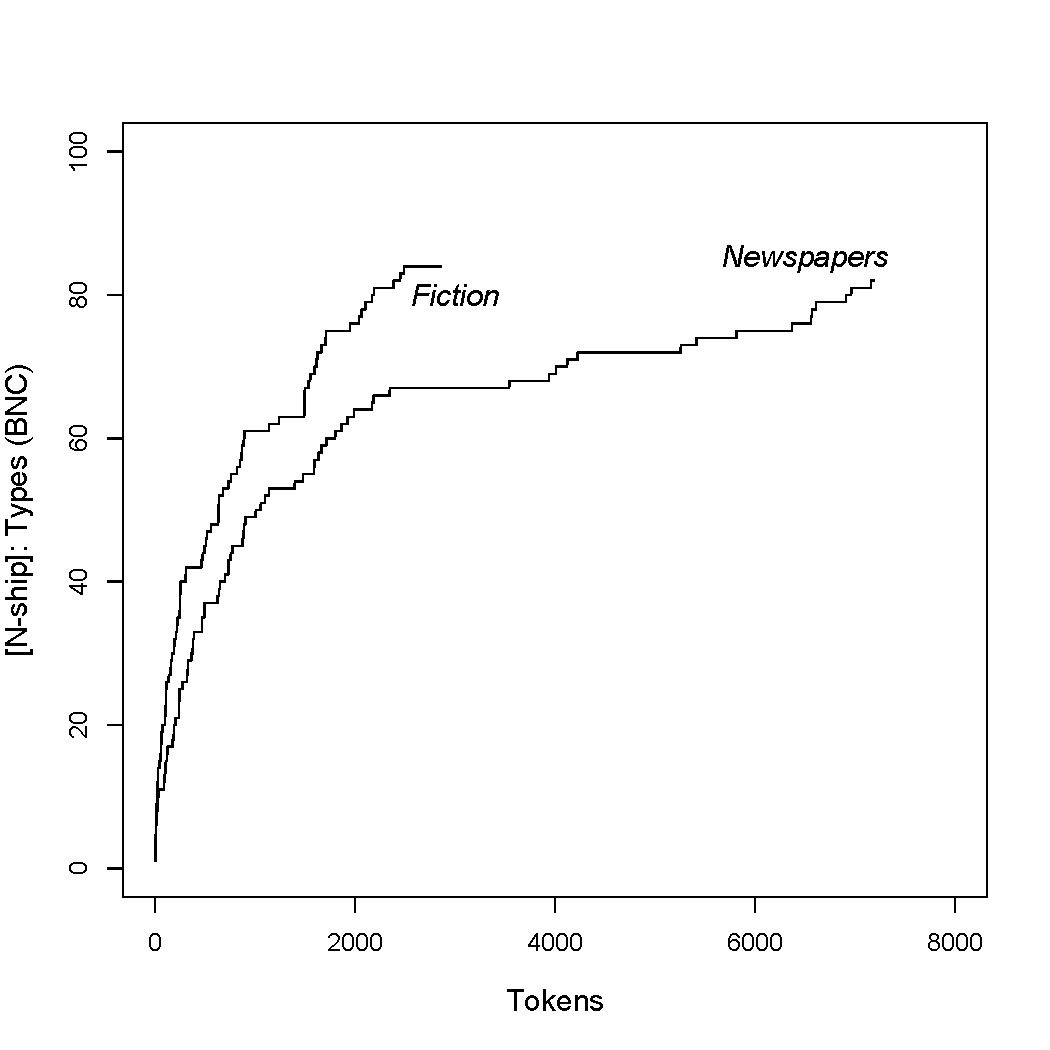
\includegraphics[width=\textwidth]{figures/genreshipfullttr}
\end{minipage}
%
\begin{minipage}{.5\textwidth}
 \centering
 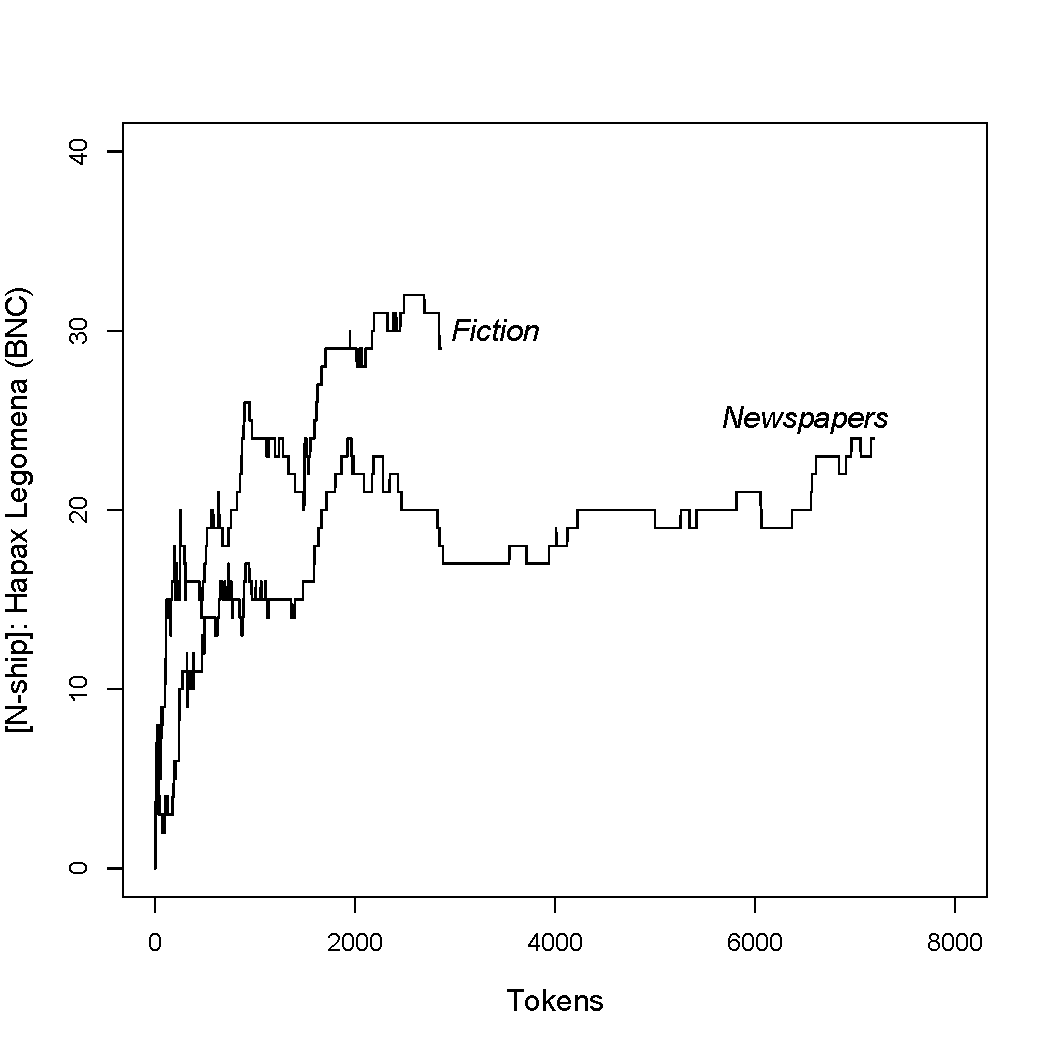
\includegraphics[width=\textwidth]{figures/genreshipfullhtr}
\end{minipage}
\end{figure}

Both the TTR \is{type-token ratio} and the HTR \is{hapax-token ratio} suggest that the suffix \is{affix} is more productive \is{productivity} in fiction: \is{literary language} the ratios rise faster in \textvv{fiction} than in \textvv{newspapers} \is{newspaper language} and remain consistently higher as we go through the two sub\hyp{}corpora. It is only when the tokens have been exhausted in the fiction subcorpus but not in the newspaper subcorpus, that the ratios in the latter slowly catch up. This broadly supports our hypothesis, but let us look at the genre \is{genre} differences more closely both qualitatively \is{qualitative research} and quantitatively. \is{quantitative research}

In order to compare the two genres \is{genre} in terms of the type\hyp{}token \is{token (instance)} \is{type-token ratio} and hapax\hyp{}token \is{hapax-token ratio} ratios, they need to have the same size. \is{corpus size} The following discussion is based on the full data from the fiction \is{literary language} subcorpus and a subsample of the newspaper \is{newspaper language} corpus that was arrived at by deleting every second, then every third and finally every 192nd example, ensuring that the hits \is{hit} in the sample are spread through the entire newspaper \is{newspaper language} subcorpus.

Let us begin by looking at the types. \is{type (category)} Overall, there are 96 different types, 48 of which occur in both samples (some examples of types that frequent in both samples are \textit{relationship} (the most frequent word in the fiction sample), \textit{championship} (the most frequent word in the news sample), \textit{friendship}, \textit{partnership}, \textit{lordship}, \textit{ownership} and \textit{membership}. In addition, there are 36 types that occur only in the prose sample (for example, \textit{churchmanship}, \textit{dreamership}, \textit{librarianship} and \textit{swordsmanship}) and 12 that occur only in the newspaper sample (for example, \textit{associateship}, \textit{draughtsmanship}, \textit{trusteeship} and \textit{sportsmanship}). The number of types \is{type (category)} exclusive to each genre \is{genre} suggests that the suffix \is{affix} is more important in \textvv{fiction} \is{literary language} than in \textvv{newspapers}. \is{newspaper language}

The TTR \is{type-token ratio} of the suffix \is{affix} in newspaper language is $\nicefrac{60}{2862} = 0.021$, and the HTR \is{hapax-token ratio} is $\nicefrac{20}{2862} = 0.007$. In contrast, the TTR in fiction is $\nicefrac{84}{2862} = 0.0294$, and the HTR is $\nicefrac{29}{2862} = 0.0101$. Although the suffix, \is{affix} as expected, \is{frequency, expected} is generally not very productive, \is{productivity} it is more productive in fiction \is{literary language} than in newspapers. \is{newspaper language} As Table \ref{tab:shipwords} shows, this difference is statistically significant in the sample ($\chi^2$ = 4.1, df = 1, p < 0.005). This corroborates our hypothesis, but note that it does not tell us whether the higher productivity \is{productivity} of \textit{-ship} is something unique about this particular morpheme, \is{morphology} or whether fiction \is{literary language} generally has more derived words due to a higher overall lexical richness. To determine this, we would have to look at more than one affix. \is{affix}

\begin{table}[!htbp]
\caption{Types with \textit{-ship} in prose fiction and newspapers}
\label{tab:shipwords}
\begin{tabular}[t]{llccr}
\lsptoprule
 & & \multicolumn{2}{c}{\textvv{Type}} & \\
 & & \textvv{new} & \textvv{$\neg$new} & Total \\
\midrule
\textvv{\makecell[lt]{Genre}}
	& \textvv{fiction}
		& \makecell[t]{\num{84}\\\small{(\num{72.00})}}
		& \makecell[t]{\num{2778}\\\small{(\num{2790.00})}}
		& \makecell[t]{\num{2862}\\} \\
	& \textvv{newspaper}
		& \makecell[t]{\num{60}\\\small{(\num{72.00})}}
		& \makecell[t]{\num{2802}\\\small{(\num{2790.00})}}
		& \makecell[t]{\num{2862}\\} \\
\midrule
	& Total
		& \makecell[t]{\num{144}}
		& \makecell[t]{\num{5580}}
		& \makecell[t]{\num{5724}} \\
\lspbottomrule
\end{tabular}
\end{table}
% me: chisq.test(matrix(c(84,60,2778,2802),ncol=2),corr=FALSE)

Let us now turn to the hapax \is{hapax legomenon} legomena. These are so rare in both genres \is{genre} that the difference in TTR \is{type-token ratio} is not statistically significant, as Table \ref{tab:shiphapaxes} shows ($\chi^2$ = 1.67, df = 1, p = 0.1966). \is{chi-square test} We would need a larger \is{corpus size} corpus to see whether the difference would at some point become significant.

\begin{table}[!htbp]
\caption{Hapaxes with \textit{-ship} in prose fiction and newspapers}
\label{tab:shiphapaxes}
\begin{tabular}[t]{llccr}
\lsptoprule
 & & \multicolumn{2}{c}{\textvv{Type}} & \\
 & & \textvv{hapax} & \textvv{$\neg$hapax} & Total \\
\midrule
\textvv{\makecell[lt]{Genre}}
	& \textvv{fiction}
		& \makecell[t]{\num{29}\\\small{(\num{24.50})}}
		& \makecell[t]{\num{2833}\\\small{(\num{2837.50})}}
		& \makecell[t]{\num{2862}\\} \\
	& \textvv{newspaper}
		& \makecell[t]{\num{20}\\\small{(\num{24.50})}}
		& \makecell[t]{\num{2842}\\\small{(\num{2837.50})}}
		& \makecell[t]{\num{2862}\\} \\
\midrule
	& Total
		& \makecell[t]{\num{49}}
		& \makecell[t]{\num{5675}}
		& \makecell[t]{\num{5724}} \\
\lspbottomrule
\end{tabular}
\end{table}
% me: chisq.test(matrix(c(29,20,2833,2842),ncol=2),corr=FALSE)

To conclude this case study, let us look at a particular problem posed by the comparison of the same suffix \is{affix} in two genres \is{genre} with respect to the HTR. \is{hapax-token ratio} At first glance -- and this is what is shown in Table \ref{tab:shiphapaxes} -- there seem to be 29 hapaxes \is{hapax legomenon} in fiction \is{literary language} and 20 in prose. However, there is some overlap: the words \textit{generalship}, \textit{headship}, \textit{managership}, \textit{ministership} and \textit{professorship} occur as hapax \is{hapax legomenon} legomena in both samples; other words that are hapaxes in one subsample occur several times in the other, such as \textit{brinkmanship}, which is a hapax in fiction but occurs twice in the newspaper sample, or \textit{acquaintanceship}, which is a hapax in the newspaper \is{newspaper language} sample but occurs 15 times in fiction.

It is not straightforwardly clear whether such cases should be treated as hapaxes. \is{hapax legomenon} If we think of the two samples as subsamples of the same corpus, it is very counterintuitive to do so. It might be more reasonable to count only those words as hapaxes whose frequency in the combined subsamples is still one. However, the notion ``hapax'' is only an operational \is{operationalization} definition for neologisms, \is{neologism} based on the hope that the number of hapaxes in a corpus (or sub\hyp{}corpus) is somehow indicative of the number of productive \is{productivity} coinages. We saw in Case Study \ref{sec:phonologicalconstraintsofify} that this is a somewhat vain hope, as the correlation \is{correlation} between neologisms and hapaxes \is{hapax legomenon} is not very impressive.

Still, if we want to use this operational \is{operationalization} definition, we have to stick with it and define hapaxes strictly relative to whatever (sub-)corpus we are dealing with. If we extend the criterion for hapax\hyp{}ship beyond one subsample to the other, why stop there? We might be even stricter and count only those words as hapaxes \is{hapax legomenon} that are still hapaxes when we take the entire BNC \is{BNC} into account. And if we take the entire BNC into account, we might as well count as hapaxes only those words that occur only once in all accessible archives of the language under investigation. This would mean that the hapaxes in any sample would overwhelmingly cease to be hapaxes -- the larger \is{corpus size} our corpus, the fewer hapaxes there will be. To illustrate this: just two words from the fiction \is{literary language} sample retain their status as hapax legomena if we search the Google Books collection: \textit{impress\hyp{}ship}, which does not occur at all (if we discount linguistic accounts which mention it, such as \citet{trips_lexical_2009}, or this book, once it becomes part of the Google Books archive), and \textit{cloudship}, which does occur, but only referring to water- or airborne vehicles. At the same time, the Google Books archive contains hundreds (if not thousands) of hapax \is{hapax legomenon} legomena that we never even notice (such as \textit{Johnship} ``the state of being the individual referred to as \textit{John}''). The idea of using hapax legomena is, essentially, that a word like \textit{mageship}, which is a hapax in the fiction \is{literary language} sample, but not in the Google Books archive, somehow stands for a word like \textit{Johnship}, which is a true hapax in the English language.

This case study has demonstrated the potential of using the TTR \is{type-token ratio} and the HTR \is{hapax-token ratio} not as a means of assessing morphological \is{morphology} richness and productivity \is{productivity} as such, but as a means of assessing genres \is{genre} with respect to their richness and productivity. It has also demonstrated some of the problems of identifying hapax \is{hapax legomenon} legomena in the context of such cross\hyp{}variety \is{language variety} comparisons. As mentioned initially, there are not too many studies of this kind, but \citet{plag_morphological_1999} presents a study of productivity \is{productivity} across written \is{medium} and spoken language that is a good starting point for anyone wanting to fill this gap.

\subsubsection{Case study: Productivity and speaker sex}
\label{sec:productivityandspeakersex}

Morphological \is{morphology} productivity \is{productivity} has not traditionally been investigated from a sociolinguistic \is{sociolinguistics} perspective, but a study by \citet{saily_variation_2011} suggests that this may be a promising field of research. S\"{a}ily investigates differences in the productivity of the suffixes \is{affix} \textit{-ness} and \textit{-ity} in the language produced by men and women in the BNC. \is{BNC} She finds no difference in productivity for \textit{-ness}, but a higher productivity \is{productivity} of \textit{-ity} in the language produced by men (cf. also \citealt{saily_comparing_2009} for a diachronic \is{diachrony} study with very similar results). She uses a sophisticated method involving the comparison of the suffixes' \is{affix} type \is{type (category)} and hapax \is{hapax legomenon} growth rates, but let us replicate \is{replicability} her study using the simple method used in the preceding case study, beginning with a comparison of type\hyp{}token \is{type-token ratio} ratios.

The BNC \is{BNC} contains substantially more speech and writing \is{medium} by male speakers than by female speakers, which is reflected in differences in the number of affix tokens \is{token (instance)} produced by men and women: for \textit{-ity}, there are \num{2562} tokens produced by women and \num{8916} tokens produced by men; for \textit{-ness}, there are 616 tokens produced by women and \num{1154} tokens produced by men (note that unlike S\"{a}ily, I excluded the words \textit{business} and \textit{witness}, since they did not seem to me to be synchronically transparent instances of the affix). \is{affix} To get samples of equal size \is{corpus size} for each affix, \is{affix} random subsamples were drawn from the tokens \is{token (instance)} produced by men.

Based on these subsamples, the type\hyp{}token \is{type-token ratio} ratios for \textit{-ity} are 0.0652 for men and 0.0777 for women; as Table \ref{tab:itysex} shows, this difference is not statistically significant ($\chi^2$ = 3.01, df = 1, p < 0.05, $\phi$ = 0.0242). \is{chi-square test}

\begin{table}[!htbp]
\caption{Types with \textit{-ity} in male and female speech (BNC)}
\label{tab:itysex}
\begin{tabular}[t]{llccr}
\lsptoprule
 & & \multicolumn{2}{c}{\textvv{Type}} & \\
 & & \textvv{new} & \textvv{seen before} & Total \\
\midrule
\textvv{\makecell[lt]{Speaker Sex}}
	& \textvv{female}
		& \makecell[t]{\num{167}\\\small{(\num{183.00})}}
		& \makecell[t]{\num{2395}\\\small{(\num{2379.00})}}
		& \makecell[t]{\num{2562}\\} \\
	& \textvv{male}
		& \makecell[t]{\num{199}\\\small{(\num{183.00})}}
		& \makecell[t]{\num{2363}\\\small{(\num{2379.00})}}
		& \makecell[t]{\num{2562}\\} \\
\midrule
	& Total
		& \makecell[t]{\num{366}}
		& \makecell[t]{\num{4758}}
		& \makecell[t]{\num{5124}} \\
\lspbottomrule
\end{tabular}
\end{table}

The type\hyp{}token \is{type-token ratio} ratios for \textit{-ness} are much higher, namely 0.1981 for women and 0.2597 for men. As Table \ref{tab:nesssex} shows, the difference is statistically significant, although the effect size \is{effect size} is weak ($\chi^2$ = 5.37, df = 1, p < 0.05, $\phi$ = 0.066).

\begin{table}[!htbp]
\caption{Types with \textit{-ness} in male and female speech (BNC)}
\label{tab:nesssex}
\begin{tabular}[t]{llccr}
\lsptoprule
 & & \multicolumn{2}{c}{\textvv{Type}} & \\
 & & \textvv{new} & \textvv{seen before} & Total \\
\midrule
\textvv{\makecell[lt]{Speaker Sex}}
	& \textvv{female}
		& \makecell[t]{\num{122}\\\small{(\num{139.00})}}
		& \makecell[t]{\num{494}\\\small{(\num{477.00})}}
		& \makecell[t]{\num{616}\\} \\
	& \textvv{male}
		& \makecell[t]{\num{156}\\\small{(\num{139.00})}}
		& \makecell[t]{\num{460}\\\small{(\num{477.00})}}
		& \makecell[t]{\num{616}\\} \\
\midrule
	& Total
		& \makecell[t]{\num{278}}
		& \makecell[t]{\num{954}}
		& \makecell[t]{\num{1232}} \\
\lspbottomrule
\end{tabular}
\end{table}
% me: chisq.test(matrix(c(122,156,494,460),ncol=2),corr=FALSE)

Note that S\"{a}ily investigates spoken \is{medium} and written language separately and she also includes social class in her analysis, so her results differ from the ones presented here; she finds a significantly lower HTR \is{hapax-token ratio} for \textit{-ness} in lower\hyp{}class women's speech in the spoken subcorpus, but not in the written one, and a significantly lower HTR for \textit{-ity} in both subcorpora. This might be due to the different methods used, or to the fact that I excluded \textit{business}, which is disproportionally frequent in male speech and writing in the BNC \is{BNC} and would thus reduce the diversity in the male sample substantially. However, the type\hyp{}based \is{type (category)} differences do not have a very impressive effect size \is{effect size} in our design \is{research design} and they are unstable across conditions in S\"{a}ily's, so perhaps they are simply not very substantial.

Let us turn to the HTR \is{hapax-token ratio} next. As before, we are defining what counts as a hapax \is{hapax legomenon} legomenon not with reference to the individual subsamples of male and female speech, but with respect to the combined sample. Table \ref{tab:ityhapaxsexlist} shows the hapaxes for \textit{-ity} in the male and female samples. The HTRs are very low, suggesting that \textit{-ity} is not a very productive \is{productivity} suffix: \is{affix} 0.0099 in female speech and 0.016 in male speech.

\begin{table}[!htbp]
\caption{Hapaxes with \textit{-ity} in sampes of male and female speech (BNC)}
\label{tab:ityhapaxsexlist}
\resizebox{0.9\textwidth}{!}{%
\begin{tabular}[t]{l}
\lsptoprule
\textvv{male speech} \\
\midrule
\makecell[tl]{
\begin{minipage}[t]{\textwidth} \raggedright
\textit{abnormality}, \textit{antiquity}, \textit{applicability}, \textit{brutality}, \textit{civility}, \textit{criminality}, \textit{deliverability}, \textit{divinity}, \textit{duplicity}, \textit{eccentricity}, \textit{eventuality}, \textit{falsity}, \textit{femininity}, \textit{fixity}, \textit{frivolity}, \textit{illegality}, \textit{impurity}, \textit{inexorability}, \textit{infallibility}, \textit{infirmity}, \textit{levity}, \textit{longevity}, \textit{mediocrity}, \textit{obesity}, \textit{perversity}, \textit{predictability}, \textit{rationality}, \textit{regularity}, \textit{reliability}, \textit{scarcity}, \textit{seniority}, \textit{serendipity}, \textit{solidity}, \textit{subsidiarity}, \textit{susceptibility}, \textit{tangibility}, \textit{verity}, \textit{versatility}, \textit{virtuality}, \textit{vitality}, \textit{voracity}
\end{minipage}} \\
\midrule
\textvv{female speech} \\
\midrule
\makecell[tl]{
\begin{minipage}[t]{\textwidth} \raggedright
\textit{absurdity}, \textit{adjustability}, \textit{admissibility}, \textit{centrality}, \textit{complicity}, \textit{effemininity}, \textit{enormity}, \textit{exclusivity}, \textit{gratuity}, \textit{hilarity}, \textit{humility}, \textit{impunity}, \textit{inquisity}, \textit{morbidity}, \textit{municipality}, \textit{originality}, \textit{progility}, \textit{respectability}, \textit{sanity}, \textit{scaleability}, \textit{sincerity}, \textit{spontaneity}, \textit{sterility}, \textit{totality}, \textit{virginity}
\end{minipage}} \\
\lspbottomrule
\end{tabular}}
\end{table}

Although the difference in HTR \is{hapax-token ratio} is relatively small, Table \ref{tab:ityhapaxfrequencies} shows that it is statistically significant, albeit again with a very weak effect size \is{effect size} ($\chi^2$ = 3.93, df = 1, p < 0.05, $\phi$ = 0.0277).

\begin{table}[!htbp]
\caption{Hapax legomena with \textit{-ity} in male and female speech (BNC)}
\label{tab:ityhapaxfrequencies}
\begin{tabular}[t]{llccr}
\lsptoprule
 & & \multicolumn{2}{c}{\textvv{Type}} & \\
 & & \textvv{hapax} & \textvv{$\neg$hapax} & Total \\
\midrule
\textvv{\makecell[lt]{Speaker Sex}}
	& \textvv{female}
		& \makecell[t]{\num{25}\\\small{(\num{33.00})}}
		& \makecell[t]{\num{2537}\\\small{(\num{2529.00})}}
		& \makecell[t]{\num{2562}\\} \\
	& \textvv{male}
		& \makecell[t]{\num{41}\\\small{(\num{33.00})}}
		& \makecell[t]{\num{2521}\\\small{(\num{2529.00})}}
		& \makecell[t]{\num{2562}\\} \\
\midrule
	& Total
		& \makecell[t]{\num{66}}
		& \makecell[t]{\num{5058}}
		& \makecell[t]{\num{5124}} \\
\lspbottomrule
\end{tabular}
\end{table}
% me: chisq.test(matrix(c(25,41,2537,2521),ncol=2),corr=FALSE)

Table \ref{tab:nesssexlist} shows the hapaxes for \textit{-ness} in the male and female samples. The HTRs \is{hapax-token ratio} are low, but much higher than for \textit{-ity}, 0.0795 for women and 0.1023 for men.

\begin{table}[!htbp]
\caption{Hapaxes with \textit{-ness} in samples of male and female speech (BNC)}
\label{tab:nesssexlist}
\resizebox*{0.9\textwidth}{!}{%
\begin{tabular}[t]{l}
\lsptoprule
\textvv{male speech} \\
\midrule
\makecell[tl]{
\begin{minipage}[t]{\textwidth} \raggedright
\textit{abjectness}, \textit{adroitness}, \textit{aloneness}, \textit{anxiousness}, \textit{awfulness}, \textit{barrenness}, \textit{blackness}, \textit{blandness}, \textit{bluntness}, \textit{carefulness}, \textit{centredness}, \textit{cleansiness}, \textit{clearness}, \textit{cowardliness}, \textit{crispness}, \textit{delightfulness}, \textit{differentness}, \textit{dizziness}, \textit{drowsiness}, \textit{dullness}, \textit{eyewitnesses}, \textit{fondness}, \textit{fulfilness}, \textit{genuineness}, \textit{godliness}, \textit{graciousness}, \textit{headedness}, \textit{heartlessness}, \textit{heinousness}, \textit{keenness}, \textit{lateness}, \textit{likeliness}, \textit{limitedness}, \textit{loudness}, \textit{mentalness}, \textit{messiness}, \textit{narrowness}, \textit{nearness}, \textit{neighbourliness}, \textit{niceness}, \textit{numbness}, \textit{pettiness}, \textit{pleasantness}, \textit{plumpness}, \textit{positiveness}, \textit{quickness}, \textit{reasonableness}, \textit{rightness}, \textit{riseness}, \textit{rudeness}, \textit{sameness}, \textit{sameyness}, \textit{separateness}, \textit{shortness}, \textit{smugness}, \textit{softness}, \textit{soreness}, \textit{springiness}, \textit{steadiness}, \textit{stubbornness}, \textit{timorousness}, \textit{toughness}, \textit{uxoriousness}
\end{minipage}} \\
\midrule
\textvv{female speech} \\
\midrule
\makecell[tl]{
\begin{minipage}[t]{\textwidth} \raggedright
\textit{ancientness}, \textit{appropriateness}, \textit{badness}, \textit{bolshiness}, \textit{chasifness}, \textit{childishness}, \textit{chubbiness}, \textit{clumsiness}, \textit{conciseness}, \textit{eagerness}, \textit{easiness}, \textit{faithfulness}, \textit{falseness}, \textit{feverishness}, \textit{fizziness}, \textit{freshness}, \textit{ghostliness}, \textit{greyness}, \textit{grossness}, \textit{grotesqueness}, \textit{heaviness}, \textit{laziness}, \textit{likeness}, \textit{mysteriousness}, \textit{nastiness}, \textit{outspokenness}, \textit{pinkness}, \textit{plainness}, \textit{politeness}, \textit{prettiness}, \textit{priggishness}, \textit{primness}, \textit{randomness}, \textit{responsiveness}, \textit{scratchiness}, \textit{sloppiness}, \textit{smoothness}, \textit{stiffness}, \textit{stretchiness}, \textit{tenderness}, \textit{tightness}, \textit{timelessness}, \textit{timidness}, \textit{ugliness}, \textit{uncomfortableness}, \textit{unpredictableness}, \textit{untidiness}, \textit{wetness}, \textit{zombieness}
\end{minipage}} \\
\lspbottomrule
\end{tabular}}
\end{table}

As Table \ref{tab:nesssexfrequencies} shows, the difference in HTRs \is{hapax-token ratio} is not statistically significant, and the effect size \is{effect size} would be very weak anyway ($\chi^2$ = 1.93, df = 1, p > 0.05, $\phi$ = 0.0395).

\begin{table}[!htbp]
\caption{Hapax legomena with \textit{-ness} in male and female speech (BNC)}
\label{tab:nesssexfrequencies}
\begin{tabular}[t]{llccr}
\lsptoprule
 & & \multicolumn{2}{c}{\textvv{Type}} & \\
 & & \textvv{hapax} & \textvv{$\neg$hapax} & Total \\
\midrule
\textvv{\makecell[lt]{Speaker Sex}}
	& \textvv{female}
		& \makecell[t]{\num{49}\\\small{(\num{56.00})}}
		& \makecell[t]{\num{567}\\\small{(\num{560.00})}}
		& \makecell[t]{\num{616}\\} \\
	& \textvv{male}
		& \makecell[t]{\num{63}\\\small{(\num{56.00})}}
		& \makecell[t]{\num{553}\\\small{(\num{560.00})}}
		& \makecell[t]{\num{616}\\} \\
\midrule
	& Total
		& \makecell[t]{\num{112}}
		& \makecell[t]{\num{1120}}
		& \makecell[t]{\num{1232}} \\
\lspbottomrule
\end{tabular}
\end{table}
% me: chisq.test(matrix(c(49,63,567,553),ncol=2),corr=FALSE)

In this case, the results correspond to S\"{a}ily's, who also finds a significant difference in productivity \is{productivity} for \textit{-ity}, but not for \textit{-ness}.

This case study was meant to demonstrate, once again, the method of comparing TTRs \is{type-token ratio} and HTRs \is{hapax-token ratio} based on samples of equal size. \is{corpus size} It was also meant to draw attention to the fact that morphological \is{morphology} productivity \is{productivity} may be an interesting area of research for variationist \is{variation} sociolinguistics; \is{sociolinguistics} however, it must be pointed out that it would be premature to conclude that men and women differ in their productive use of particular affixes; \is{affix} as S\"{a}ily herself points out, men and women are not only represented unevenly in quantitative \is{quantitative research} terms (with a much larger proportion of male language included in the BNC), \is{BNC} but also in qualitative terms (the language varieties \is{language variety} with which they are represented differ quite strikingly). Thus, this may actually be another case of different degrees of productivity \is{productivity} in different language varieties (which we investigated in the preceding case study).

\chapter{Text}
\label{ch:text}

As mentioned repeatedly, linguistic corpora, by their nature, consist of word forms, while other levels of linguistic representation are not represented unless the corresponding annotations \is{annotation} are added. In written \is{medium} corpora, there is one level other than the lexical that is (or can be) directly represented: the text. Well\hyp{}constructed linguistic corpora typically consist of (samples from) individual texts, whose meta\hyp{}information (author, title, original place and context of publication, etc.) are known. There is a substantial body of corpus\hyp{}linguistic research based on designs \is{research design} that combine the two inherently represented variables \textsc{Word (Form)} and \textsc{Text}; such designs may be concerned with the occurrence of words in individual texts, or, more typically, with the occurrence of words in clusters of texts belonging to the same language variety \is{language variety} (defined by topic, genre, \is{genre} function, etc.).

Texts are, of course, produced by speakers, and depending on how much and what kind of information about these speakers is available, we can also cluster texts according to demographic \is{demography} variables such as dialect, socioeconomic status, gender, age, \is{age} political or religious affiliation, etc. (as we have done in many of the examples in earlier chapters). In these cases, quantitative \is{quantitative research} corpus linguistics is essentially a variant of sociolinguistics, \is{sociolinguistics} differing mainly in that the linguistic phenomena it pays most attention to are not necessarily those most central to sociolinguistic \is{sociolinguistics} research in general.

\section{Keyword analysis}
\label{sec:keywordanalysis}

In the investigation of relationships between words (or other units of language structure) and texts (or clusters of texts), researchers frequently use a method referred to as \is{keyword analysis} \textit{keyword analysis}.\footnote{The term \textit{keyword} is frequently spelled as two words (\textit{key word}) or with a hyphen (\textit{key\hyp{}word}). I have chosen the spelling as a single word here because it seems simplest (at least to me, as a native writer of German, where compounds are always spelled as single words).} The term was originally used in contexts where cultural \is{culture} values and practices were studied through particular lexical items (cf. \citealt{williams_keywords:_1976}, \citealt{wierzbicka_cross-cultural_2003}); in corpus linguistics, it is used in a related but slightly broader sense of words that are characteristic of a particular text, language variety \is{language variety} or demographic \is{demography} in the sense that they occur with ``unusual frequency in a given text'' or set of texts, where ``unusual'' means high ``by comparison with a reference corpus of some kind'' \citep[236]{scott_pc_1997}.

In other words, the corpus\hyp{}linguistic identification of keywords \is{keyword analysis} is analogous to the identification of differential collocates, \is{collocation} except that it analyses the association \is{association} of a word W to a particular text (or collection of texts) T in comparison to the language as a whole (as represented by the reference corpus, which is typically a large, \is{corpus size} balanced corpus). Table \ref{tab:keywordanalysis} shows this schematically.

\begin{table}[!htbp]
\caption{A generic 2\hyp{}by\hyp{}2 table for keyword analysis}
\label{tab:keywordanalysis}
\begin{tabular}[t]{llccc}
\lsptoprule
 & & \multicolumn{2}{c}{\textvv{Text}} & \\
 & & \textvv{text/corpus t} & \textvv{reference corpus} & Total \\
\midrule
\textvv{\makecell[lt]{Word}}
	& \textvv{word w}
		& \makecell[t]{O\textsubscript{11}}
		& \makecell[t]{O\textsubscript{12}}
		& \makecell[t]{R\textsubscript{1}} \\
	& \textvv{other words}
		& \makecell[t]{O\textsubscript{21}}
		& \makecell[t]{O\textsubscript{22}}
		& \makecell[t]{R\textsubscript{2}} \\
\midrule
	& Total
		& \makecell[t]{C\textsubscript{1}}
		& \makecell[t]{C\textsubscript{2}}
		& \makecell[t]{N} \\
\lspbottomrule
\end{tabular}
\end{table}

Just like collocation \is{collocation} analysis, keyword \is{keyword analysis} analysis is most often applied inductively, \is{induction} but there is nothing that precludes a deductive \is{deduction} design \is{research design} if we have hypotheses about the over- or underrepresentation of particular lexical items in a particular text or collection of texts. In either case, we have two nominal \is{nominal data} variables: \textsc{Keyword} (with the individual \textsc{words} as values) and \textsc{Text} (with the values \textsc{text} and \textsc{reference corpus}).

If keyword \is{keyword analysis} analysis is applied to a single text, the aim is typically to identify either the topic area or some stylistic \is{style} property of that text. When applied to text categories, the aim is typically to identify general lexical and\slash or grammatical \is{grammar} properties of the language variety \is{language variety} represented by the text categories.

As a first example of the kind of results that keyword \is{keyword analysis} analysis yields, consider Table \ref{tab:threetextsfreq}, which shows the 20 most frequent tokens \is{token (instance)} (including punctuation marks) in the LOB \is{LOB} corpus and two individual texts (all words were converted to lower case).

\begin{table}[!htbp]
\caption{Most frequent words in three texts (relative frequencies)}
\label{tab:threetextsfreq}
\resizebox{.7\textwidth}{!}{%
\begin{tabular}[t]{lr|lr|lr}
\lsptoprule
\multicolumn{2}{c|}{\textvv{LOB}} & \multicolumn{2}{c|}{\textvv{Text A}} & \multicolumn{2}{c}{\textvv{Text B}} \\
\midrule
\textit{the} & \num[round-mode=places,round-precision=6]{0.0590} & \textit{the} & \num[round-mode=places,round-precision=6]{0.0610} & \textit{the} & \num[round-mode=places,round-precision=6]{0.0585} \\
\textit{,} & \num[round-mode=places,round-precision=6]{0.0471} & \textit{,} & \num[round-mode=places,round-precision=6]{0.0584} & \textit{.} & \num[round-mode=places,round-precision=6]{0.0560} \\
\textit{.} & \num[round-mode=places,round-precision=6]{0.0435} & \textit{.} & \num[round-mode=places,round-precision=6]{0.0449} & \textit{,} & \num[round-mode=places,round-precision=6]{0.0452} \\
\textit{of} & \num[round-mode=places,round-precision=6]{0.0309} & \textit{in} & \num[round-mode=places,round-precision=6]{0.0383} & \textit{of} & \num[round-mode=places,round-precision=6]{0.0258} \\
\textit{and} & \num[round-mode=places,round-precision=6]{0.0241} & \textit{of} & \num[round-mode=places,round-precision=6]{0.0340} & \textit{a} & \num[round-mode=places,round-precision=6]{0.0231} \\
\textit{to} & \num[round-mode=places,round-precision=6]{0.0231} & \textit{and} & \num[round-mode=places,round-precision=6]{0.0256} & \textit{to} & \num[round-mode=places,round-precision=6]{0.0208} \\
\textit{a} & \num[round-mode=places,round-precision=6]{0.0197} & \textit{$($} & \num[round-mode=places,round-precision=6]{0.0137} & \textit{he} & \num[round-mode=places,round-precision=6]{0.0192} \\
\textit{in} & \num[round-mode=places,round-precision=6]{0.0184} & \textit{$)$} & \num[round-mode=places,round-precision=6]{0.0137} & \textit{``} & \num[round-mode=places,round-precision=6]{0.0150} \\
\textit{that} & \num[round-mode=places,round-precision=6]{0.0098} & \textit{at} & \num[round-mode=places,round-precision=6]{0.0123} & \textit{''} & \num[round-mode=places,round-precision=6]{0.0149} \\
\textit{is} & \num[round-mode=places,round-precision=6]{0.0096} & \textit{a} & \num[round-mode=places,round-precision=6]{0.0119} & \textit{and} & \num[round-mode=places,round-precision=6]{0.0148} \\
\textit{was} & \num[round-mode=places,round-precision=6]{0.0092} & \textit{to} & \num[round-mode=places,round-precision=6]{0.0117} & \textit{his} & \num[round-mode=places,round-precision=6]{0.0140} \\
\textit{it} & \num[round-mode=places,round-precision=6]{0.0091} & \textit{was} & \num[round-mode=places,round-precision=6]{0.0116} & \textit{was} & \num[round-mode=places,round-precision=6]{0.0138} \\
\textit{`} & \num[round-mode=places,round-precision=6]{0.0087} & \textit{neosho} & \num[round-mode=places,round-precision=6]{0.0112} & \textit{in} & \num[round-mode=places,round-precision=6]{0.0112} \\
\textit{'} & \num[round-mode=places,round-precision=6]{0.0085} & \textit{were} & \num[round-mode=places,round-precision=6]{0.0110} & \textit{that} & \num[round-mode=places,round-precision=6]{0.0110} \\
\textit{for} & \num[round-mode=places,round-precision=6]{0.0080} & \textit{species} & \num[round-mode=places,round-precision=6]{0.0078} & \textit{had} & \num[round-mode=places,round-precision=6]{0.0099} \\
\textit{he} & \num[round-mode=places,round-precision=6]{0.0078} & \textit{station} & \num[round-mode=places,round-precision=6]{0.0071} & \textit{hume} & \num[round-mode=places,round-precision=6]{0.0081} \\
\textit{i} & \num[round-mode=places,round-precision=6]{0.0066} & \textit{river} & \num[round-mode=places,round-precision=6]{0.0067} & \textit{on} & \num[round-mode=places,round-precision=6]{0.0078} \\
\textit{as} & \num[round-mode=places,round-precision=6]{0.0063} & \textit{that} & \num[round-mode=places,round-precision=6]{0.0065} & \textit{it} & \num[round-mode=places,round-precision=6]{0.0068} \\
\textit{with} & \num[round-mode=places,round-precision=6]{0.0062} & \textit{by} & \num[round-mode=places,round-precision=6]{0.0064} & \textit{--} & \num[round-mode=places,round-precision=6]{0.0063} \\
\textit{be} & \num[round-mode=places,round-precision=6]{0.0062} & \textit{1959} & \num[round-mode=places,round-precision=6]{0.0062} & \textit{as} & \num[round-mode=places,round-precision=6]{0.0063} \\
\lspbottomrule
\end{tabular}}
\end{table}
% me: all tokens, case insensitive

As we can see, the differences are relatively small, as all lists are dominated by frequent function words and punctuation marks. Ten of these occur on all three lists (\textit{a}, \textit{and}, \textit{in}, \textit{of}, \textit{that}, \textit{the}, \textit{to}, \textit{was}, the comma and the period), and another six occur on two of them (\textit{as}, \textit{he}, \textit{it}, \textit{on}, and opening and closing quotation marks -- although the latter are single quotation marks in the case of LOB \is{LOB} and double quotation marks in the case of Text B). Even the types \is{type (category)} that occur only once are mostly uninformative with respect to the language variety \is{language variety} (or text category) we may be dealing with (\textit{1959}, \textit{at}, \textit{by}, \textit{for}, \textit{had}, \textit{is}, \textit{with}, the hyphen and opening and closing parentheses). The only exceptions are four content words in Text A: \textit{Neosho}, \textit{river}, \textit{species}, \textit{station} -- these suggest that the text is about the \textit{Neosho} river and perhaps that it deals with biology (as suggested by the word \textit{species}).

Applying keyword \is{keyword analysis} analysis to each text or collection of texts allows us to identify the words that differ most significantly in frequency from the reference corpus, telling us how the text in question differs lexically from the (written) \is{medium} language of its time as a whole. Table \ref{tab:fishreportkey} lists the keywords \is{keyword analysis} for Text A.

\begin{table}[!htbp]
\caption{Keywords in a report on fish populations}
\label{tab:fishreportkey}
\resizebox{\textwidth}{!}{%
\begin{tabular}[t]{l *{2}{S[table-format=4]} *{2}{S[table-format=8]} S}
\lsptoprule
\multicolumn{1}{c}{\makecell[tc]{\textvv{Keyword}}} & \multicolumn{1}{c}{\makecell[tc]{Frequency \\ in \textvv{report}}} & \multicolumn{1}{c}{\makecell[tc]{Frequency \\ in \textvv{LOB}}} & \multicolumn{1}{c}{\makecell[tc]{Other words \\ in \textvv{report}}} & \multicolumn{1}{c}{\makecell[tc]{Other words \\ in \textvv{LOB}}} & \multicolumn{1}{c}{\makecell[tc]{G\textsuperscript{2}}} \\
\midrule
\textit{neosho} & 277 & 0 & 24525 & 1157496 & 2143.85754676855 \\
\textit{species} & 194 & 25 & 24608 & 1157471 & 1346.34569133827 \\
\textit{station} & 177 & 119 & 24625 & 1157377 & 975.304736947018 \\
\textit{river} & 165 & 104 & 24637 & 1157392 & 921.714686756413 \\
\textit{1957} & 137 & 57 & 24665 & 1157439 & 827.015414144296 \\
\textit{1959} & 153 & 124 & 24649 & 1157372 & 807.663174449525 \\
\textit{kansas} & 107 & 2 & 24695 & 1157494 & 807.539431152387 \\
\textit{cygnes} & 94 & 0 & 24708 & 1157496 & 726.835944146123 \\
\textit{marais} & 94 & 1 & 24708 & 1157495 & 715.780996710436 \\
\textit{catfish} & 90 & 0 & 24712 & 1157496 & 695.892508588732 \\
\textit{des} & 97 & 29 & 24705 & 1157467 & 615.323312002121 \\
\textit{fish} & 121 & 121 & 24681 & 1157375 & 605.360202906426 \\
\textit{upper} & 103 & 61 & 24699 & 1157435 & 582.56385976272 \\
\textit{abundance} & 81 & 7 & 24721 & 1157489 & 577.702494651473 \\
\textit{$($} & 340 & 2902 & 24462 & 1154594 & 577.40748732819 \\
\textit{$)$} & 340 & 2926 & 24462 & 1154570 & 573.116609220526 \\
\textit{channel} & 88 & 22 & 24714 & 1157474 & 571.2623085742 \\
\textit{shiner} & 75 & 3 & 24727 & 1157493 & 554.561054361179 \\
\textit{lower} & 103 & 120 & 24699 & 1157376 & 493.684469416984 \\
\textit{minnow} & 63 & 1 & 24739 & 1157495 & 476.7977064622 \\
\lspbottomrule
\end{tabular}}
\end{table}
% me: LOB_LEGACY vs. FISHREPORT, all tokens, case insensitive

The keywords \is{keyword analysis} now convey a very specific idea of what the text is about: there are two proper names of rivers (the \textit{Neosho} already seen on the frequency \is{frequency} list and the \textit{Marais des Cygnes}, represented by its constituents \textit{Cygnes}, \textit{Marais} and \textit{des}), and there are a number of words for specific species of fish as well as the words \textit{river} and \textit{channel}.

The text is clearly about fish in the two rivers. The occurrence of the words \textit{station} and \textit{abundance} suggests a research context, which is supported by the occurrence of two dates and opening and closing parentheses (which are often used in scientific texts to introduce references). The text in question is indeed a scientific report on fish populations: \textit{Fish Populations, Following a Drought, In the Neosho and Marais des Cygnes Rivers of Kansas} (available via Project Gutenberg and in the Supplementary Online Material, file TXQP). Note that the occurrence of some tokens \is{token (instance)} (such as the dates and the parentheses) may be characteristic of a language variety \is{language variety} rather than an individual text, a point we will return to below.

Next, consider Table \ref{tab:scifikey}, which lists the keywords \is{keyword analysis} for Text B. Three things are noticeable: the keyness \is{keyness} of a number of words that are most likely proper names (\textit{Hume}, \textit{Vye}, \textit{Rynch}, \textit{Wass}, \textit{Brodie} and \textit{Jumala}), pronouns \is{pronoun} (\textit{he}, \textit{his}) and punctuation marks indicative of direct speech (the quotation marks and the exclamation mark).

\begin{table}[!htbp]
\caption{Keywords in a science fiction novel}
\label{tab:scifikey}
\resizebox{\textwidth}{!}{%
\begin{tabular}[t]{l *{2}{S[table-format=4]} *{2}{S[table-format=8]} S}
\lsptoprule
\multicolumn{1}{c}{\makecell[tc]{\textvv{Keyword}}} & \multicolumn{1}{c}{\makecell[tc]{Frequency \\ in \textvv{novel}}} & \multicolumn{1}{c}{\makecell[tc]{Frequency \\ in \textvv{LOB}}} & \multicolumn{1}{c}{\makecell[tc]{Other words \\ in \textvv{novel}}} & \multicolumn{1}{c}{\makecell[tc]{Other words \\ in \textvv{LOB}}} & \multicolumn{1}{c}{\makecell[tc]{G\textsuperscript{2}}} \\
\midrule
\textit{``} & 604 & 77 & 24198 & 1157419 & 4205.14307110206 \\
\textit{''} & 601 & 121 & 24201 & 1157375 & 4011.51063154168 \\
\textit{hume} & 325 & 2 & 24477 & 1157494 & 2491.68595753249 \\
\textit{--} & 254 & 0 & 24548 & 1157496 & 1965.61541621278 \\
\textit{vye} & 228 & 0 & 24574 & 1157496 & 1764.1751305293 \\
\textit{rynch} & 134 & 0 & 24668 & 1157496 & 1036.34007757997 \\
\textit{.} & 2252 & 50324 & 22550 & 1107172 & 1000.71159535114 \\
\textit{he} & 772 & 9068 & 24030 & 1148428 & 952.737784983041 \\
\textit{wass} & 100 & 0 & 24702 & 1157496 & 773.253475159535 \\
\textit{his} & 565 & 6272 & 24237 & 1151224 & 740.624919140107 \\
\textit{'s} & 214 & 1177 & 24588 & 1156319 & 510.858785197556 \\
\textit{the} & 2352 & 68350 & 22450 & 1089146 & 475.704566275507 \\
\textit{had} & 397 & 5473 & 24405 & 1152023 & 398.127782320442 \\
\textit{brodie} & 44 & 0 & 24758 & 1157496 & 340.13407369537 \\
\textit{was} & 556 & 10685 & 24246 & 1146811 & 327.11360582672 \\
\textit{,} & 1820 & 54548 & 22982 & 1102948 & 319.741050413579 \\
\textit{flitter} & 41 & 0 & 24761 & 1157496 & 316.938253211963 \\
\textit{a} & 931 & 22857 & 23871 & 1134639 & 313.15958677858 \\
\textit{hunter} & 43 & 12 & 24759 & 1157484 & 275.204326155239 \\
\textit{could} & 171 & 1741 & 24631 & 1155755 & 244.217436561136 \\
\lspbottomrule
\end{tabular}}
\end{table}
% me: LOB_LEGACY vs. STARHUNTER, all tokens, case insensitive

This does not tell us anything about this particular text, but taken together, these pieces of evidence point to a particular genre: \is{genre} narrative text (novels, \is{literary language} short stories, etc.). The few potential content words suggest a particular sub\hyp{}genre: the archaic \textit{hunter} in combination with the unusual word \textit{flitter} is suggestive of fantasy or science fiction. If we were to include the next twenty most strongly associated \is{association} nouns, \is{noun} we would find \textit{patrol}, \textit{camp}, \textit{needler}, \textit{safari}, \textit{guild}, \textit{tube}, \textit{planet} and \textit{out\hyp{}hunter}, which corroborate the impression that we are dealing with a science\hyp{}fiction \is{literary language} novel. And indeed, the text in question is the science\hyp{}fiction novel \textit{Starhunter} by Andre Alice Norton (available via Project Gutenberg in the Supplementary Online Material, file TXQP).

Again, the keywords \is{keyword analysis} identified are a mixture of topical markers and markers for the language variety \is{language variety} (in this case, the genre) \is{genre} of the text, so even a study of the keywords of single texts provides information about more general linguistic properties of the text in question as well as its specific topic. But keyword \is{keyword analysis} analysis reveals its true potential when we apply it to clusters of texts, as in the case studies in the next section.

\section{Case studies}
\label{sec:keywordcasestudies}

\subsection{Language Variety}
\label{sec:texttype}

Keyword \is{keyword analysis} analysis has been applied to a wide range of language varieties \is{language variety} defined by topic area (e.g. travel writing), genre \is{genre} (e.g. news reportage) \is{newspaper language} or both (e.g. history textbooks) (see the contributions in \citealt{bondi_keyness_2010} for recent examples). Here, we will look at two case studies of scientific language.

\subsubsection{Case study: Keywords in scientific writing}
\label{sec:keywordsinscientificwriting}

There are a number of keyword\hyp{}based \is{keyword analysis} analyses of academic \is{academic language} writing (cf., for example, \citealt{scott_textual_2006} on literary \is{literary language} criticism, \citealt{romer_applying_2010} on academic student essays). Instead of replicating \is{replicability} one of these studies in detail, let us look more generally at the Learned \is{academic language} and Scientific Writing section of the LOB \is{LOB} (Section J), using the rest of the corpus (all sections except Section J) as a reference corpus. Table \ref{tab:learnedlobbkey} shows the keywords \is{keyword analysis} for this section.

\begin{table}[!htbp]
\caption{Key words in the Learned and Scientific Writing section of LOB}
\label{tab:learnedlobbkey}
\resizebox{\textwidth}{!}{%
\begin{tabular}[t]{l *{2}{S[table-format=4]} *{2}{S[table-format=8]} S}
\lsptoprule
\multicolumn{1}{c}{\makecell[tc]{\textvv{Keyword}}} & \multicolumn{1}{c}{\makecell[tc]{Frequency \\ in \textvv{lob j}}} & \multicolumn{1}{c}{\makecell[tc]{Frequency in \\ \textvv{other sections}}} & \multicolumn{1}{c}{\makecell[tc]{Other words \\ in \textvv{lob j}}} & \multicolumn{1}{c}{\makecell[tc]{Other words in \\ \textvv{other sections}}} & \multicolumn{1}{c}{\makecell[tc]{G\textsuperscript{2}}} \\
\midrule
\textit{of} & 7899 & 27846 & 173017 & 948734 & 1065.04638043146 \\
\textit{@} & 313 & 36 & 180603 & 976544 & 942.81564402586 \\
\textit{$($} & 1099 & 1803 & 179817 & 974777 & 844.527153580497 \\
\textit{$)$} & 1101 & 1825 & 179815 & 974755 & 834.66176070663 \\
\textit{the} & 13125 & 55225 & 167791 & 921355 & 666.504967418239 \\
\textit{=} & 102 & 3 & 180814 & 976577 & 352.442427273622 \\
\textit{is} & 2482 & 8619 & 178434 & 967961 & 348.237314932627 \\
\textit{in} & 4332 & 16917 & 176584 & 959663 & 345.369311367296 \\
\textit{fig} & 113 & 31 & 180803 & 976549 & 280.033479312755 \\
\textit{data} & 88 & 8 & 180828 & 976572 & 274.334471554413 \\
\textit{equation} & 72 & 0 & 180844 & 976580 & 267.285514550513 \\
\textit{values} & 111 & 47 & 180805 & 976533 & 235.702271725609 \\
\textit{oxygen} & 63 & 2 & 180853 & 976578 & 216.689012985925 \\
\textit{sodium} & 60 & 2 & 180856 & 976578 & 205.743466498154 \\
\textit{results} & 121 & 81 & 180795 & 976499 & 204.674997380884 \\
\textit{obtained} & 98 & 49 & 180818 & 976531 & 193.329942125712 \\
\textit{experiments} & 72 & 15 & 180844 & 976565 & 192.395828660292 \\
\textit{\%} & 77 & 22 & 180839 & 976558 & 188.442264502073 \\
\textit{model} & 83 & 33 & 180833 & 976547 & 180.801823144271 \\
\textit{solution} & 96 & 53 & 180820 & 976527 & 180.42840041207 \\
\lspbottomrule
\end{tabular}}
\end{table}
% me: LOB_LEGACY J against all other sections, all tokens, case insensitive

It is immediately obvious from the preponderance of scientific terminology that we are dealing with Scientific English -- there are general scientific terms like \textit{fig(ure)}, \textit{data} \textit{experiment} or \textit{model}, mathematical terms and symbols (\textit{equation}, \textit{values}, the equals and percent signs), and a few words from chemistry (\textit{oxygen}, \textit{sodium}) (the reason the @ sign appears on this list is because it is used to mark places in the corpus where material such as mathematical formulae and operators have been deleted).

It may not be surprising that scientific terminology dominates in a corpus of Scientific English, but it demonstrates that keyword \is{keyword analysis} analysis works. Given this, we can make some more profound observations on the basis of the list in Table \ref{tab:learnedlobbkey}. For example, we observe that certain kinds of punctuation are typical of academic \is{academic language} writing in general (such as the parentheses, which we already suspected based on the analysis of the fish population report in Section \ref{sec:keywordanalysis} above). Even more interestingly, keyword \is{keyword analysis} analysis can reveal function words that are characteristic for a particular language variety \is{language variety} and thus give us potential insights into grammatical \is{grammar} structures that may be typical for it; for example, \textit{is}, \textit{the} and \textit{of} are among the most significant keywords of Scientific English. The last two are presumably related to the ``nominal'' \is{noun} style \is{style} that is known to characterize academic \is{academic language} texts, while the higher\hyp{}than\hyp{}normal frequency \is{frequency} of \textit{is} may be due to the prevalence of definitions, statements of equivalence, etc. This (and other observations made on the basis of keyword \is{keyword analysis} analysis) would of course have to be followed up by more detailed analyses of the function these words serve -- but keyword analysis tells us what words are likely to be interesting to investigate.

\subsubsection{Case study: [a + \_\_ + of] in Scientific English}
\label{sec:anofinmedicalresearchpapers}

Of course, keyword \is{keyword analysis} analysis is not the only way to study lexical characteristics of language varieties. \is{language variety} In principle, any design \is{research design} studying the interaction of lexical items with other units of linguistic structure can also be applied to specific language varieties.

For example, \citet{marco_collocational_2000} investigates collocational \is{collocation} frameworks \is{collocational framework} (see Chapter \ref{ch:grammar}, Section \ref{sec:collocationalframeworksandgrammarpatterns}) in medical research papers. While this may not sound particularly interesting at first glance, it turns out that even highly frequent frameworks like [\textit{a \_\_ of}] are filled by completely different items from those found in the language as a whole, which is important for many applied purposes (such as language teaching or machine processing of language), but which also shows just how different language varieties \is{language variety} can actually be. Since Marco's corpus is not publicly available and the Learned \is{academic language} and Scientific Writing section of LOB \is{LOB} is too small for this kind of analysis, let us use the Written Academic subsection of the BNC Baby. \is{BNC Baby} Table \ref{tab:anoflearnedfreq} shows the 15 most strongly associated \is{association} collocates \is{collocation} in the framework \is{collocational framework} [\textit{a \_\_ of}], i.e. the words whose frequency \is{frequency} of occurrence inside this framework differs most significantly from their frequency of occurrence outside of this framework in the same corpus section.

\begin{table}[!htbp]
\caption{Collocates of the framework [\textit{a} \_\_ \textit{of}] in the Written Academic subsection of BNC Baby}
\label{tab:anoflearnedfreq}
\resizebox{\textwidth}{!}{%
\begin{tabular}[t]{l *{2}{S[table-format=4]} *{2}{S[table-format=8]} S}
\lsptoprule
\multicolumn{1}{c}{\makecell[tc]{\textvv{Collocate}}} & \multicolumn{1}{c}{\makecell[tc]{Frequency in \\ $[$\textit{a} \_\_ \textit{of}$]$ }} & \multicolumn{1}{c}{\makecell[tc]{Frequency in \\ other contexts}} & \multicolumn{1}{c}{\makecell[tc]{Other words in \\ $[$\textit{a} \_\_ \textit{of}$]$}} & \multicolumn{1}{c}{\makecell[tc]{Other words in \\ other contexts}} & \multicolumn{1}{c}{\makecell[tc]{G\textsuperscript{2}}} \\
\midrule
\textit{number} & 272 & 805 & 2965 & 1138862 & 2001.8435699171 \\
\textit{series} & 99 & 203 & 3138 & 1139464 & 783.667251087437 \\
\textit{variety} & 82 & 163 & 3155 & 1139504 & 652.774047772446 \\
\textit{result} & 98 & 425 & 3139 & 1139242 & 650.603952199947 \\
\textit{matter} & 61 & 190 & 3176 & 1139477 & 439.564574439839 \\
\textit{function} & 65 & 319 & 3172 & 1139348 & 416.521135032684 \\
\textit{range} & 66 & 388 & 3171 & 1139279 & 401.451789166953 \\
\textit{set} & 59 & 442 & 3178 & 1139225 & 332.637399492872 \\
\textit{lot} & 36 & 61 & 3201 & 1139606 & 295.189976627841 \\
\textit{form} & 65 & 933 & 3172 & 1138734 & 288.418237292356 \\
\textit{combination} & 34 & 115 & 3203 & 1139552 & 239.888093602344 \\
\textit{measure} & 35 & 139 & 3202 & 1139528 & 237.133277709872 \\
\textit{consequence} & 33 & 109 & 3204 & 1139558 & 234.178040913071 \\
\textit{piece} & 29 & 73 & 3208 & 1139594 & 219.153519937284 \\
\textit{group} & 43 & 605 & 3194 & 1139062 & 192.121246046857 \\
\textit{list} & 28 & 125 & 3209 & 1139542 & 183.847199884568 \\
\textit{source} & 26 & 161 & 3211 & 1139506 & 155.380824149027 \\
\textit{way} & 41 & 870 & 3196 & 1138797 & 152.056359343873 \\
\textit{study} & 36 & 594 & 3201 & 1139073 & 150.153705753867 \\
\textit{sense} & 29 & 294 & 3208 & 1139373 & 147.065016772325 \\
\lspbottomrule
\multicolumn{6}{l}{\scriptsize{Supplementary Online Material: FXHV}} \\ %OSM
\end{tabular}}
\end{table}
% me: collexeme analysis, case insensitive

If we compare the result in Table \ref{tab:anoflearnedfreq} to that in Table \ref{tab:axofcollframe} in Chapter \ref{ch:grammar}, we notice clear differences between the use of this framework \is{collocational framework} in academic \is{academic language} texts and the language as a whole; for example, \textit{lot}, which is most strongly associated \is{association} with the framework in the general language occurs in 9th position, while the top collocates \is{collocation} of the framework \is{collocational framework} are more precise quantification \is{quantitative research} terms like \textit{number} or \textit{series}, and general scientific terms like \textit{result} and \textit{function}.

However, the two lists -- that in Table \ref{tab:axofcollframe} and that presented here -- were derived independently from different corpora, making it difficult to determine the true extent of the differences. In particular, in each of the two corpora the words in the pattern compete with the words outside of the pattern, which are obviously from the same discourse domains. To get a clearer idea of the different function(s) that a pattern might play in two different language varieties, \is{language variety} we can combine collocational \is{collocation} framework \is{collocational framework} analysis and keyword \is{keyword analysis} analysis: we extract \is{retrieval} all words occurring in a collocational framework (or grammar \is{grammar} pattern, \is{grammar pattern} construction, etc.) in a particular language variety, \is{language variety} and compare them to the words occurring in the same pattern in a reference corpus (\citealt{stefanowitsch_lot_2017} refers to this mix of keyword \is{keyword analysis} and collostructional \is{collostructional analysis} analysis as ``textually\hyp{}distinctive [i.e., differential] collexeme \is{collexeme, differential} analysis'').

Table \ref{tab:anoflearnedkey} shows the result of such an analysis in the BNC Baby, \is{BNC Baby} comparing words occurring in the framework \is{collocational framework} [\textit{a(n)} \_ \textit{of}] in the Written Academic \is{academic language} section to the words occurring in the same pattern in the rest of the corpus (all sections other than Written Academic).

\begin{table}[!htbp]
\caption{Textually differential collexemes in the framework $[$\textit{a} + \_ + \textit{of}$]$ in the Written Academic section of BNC Baby compared to all other sections}
\label{tab:anoflearnedkey}
\resizebox{\textwidth}{!}{%
\begin{tabular}[t]{l *{2}{S[table-format=4]} *{2}{S[table-format=8]} S}
\lsptoprule
\multicolumn{1}{c}{\makecell[tc]{\textvv{Keyword}}} & \multicolumn{1}{c}{\makecell[tc]{Frequency in \\ $[$\textit{a} + \_ + \textit{of}$]$ \\ in Wrt. Acad.}} & \multicolumn{1}{c}{\makecell[tc]{Frequency in \\ $[$\textit{a} + \_ + \textit{of}$]$ \\ in other sections}} & \multicolumn{1}{c}{\makecell[tc]{Frequency in \\ other contexts \\ in Wrt. Acad.}} & \multicolumn{1}{c}{\makecell[tc]{Frequency in \\ other contexts \\ in other sections}} & \multicolumn{1}{c}{\makecell[tc]{G\textsuperscript{2}}} \\
\midrule
\textit{number} & 272 & 151 & 1139395 & 3505016 & 298.079769744575 \\
\textit{function} & 65 & 0 & 1139602 & 3505167 & 182.65533525054 \\
\textit{form} & 65 & 17 & 1139602 & 3505150 & 108.524115849062 \\
\textit{variety} & 82 & 35 & 1139585 & 3505132 & 107.360346596459 \\
\textit{range} & 66 & 20 & 1139601 & 3505147 & 103.441601338926 \\
\textit{result} & 98 & 64 & 1139569 & 3505103 & 94.0314553677179 \\
\textit{series} & 99 & 81 & 1139568 & 3505086 & 76.0732182844072 \\
\textit{study} & 36 & 6 & 1139631 & 3505161 & 70.0906119931282 \\
\textit{measure} & 35 & 6 & 1139632 & 3505161 & 67.592867724927 \\
\textit{consequence} & 33 & 5 & 1139634 & 3505162 & 65.9544448366265 \\
\textit{set} & 59 & 32 & 1139608 & 3505135 & 65.7910710487631 \\
\textit{solution} & 23 & 0 & 1139644 & 3505167 & 64.6312481948337 \\
\textit{critique} & 23 & 1 & 1139644 & 3505166 & 56.8804233749769 \\
\textit{theory} & 20 & 0 & 1139647 & 3505167 & 56.2010456562647 \\
\textit{process} & 26 & 5 & 1139641 & 3505162 & 48.4847755359066 \\
\textit{matrix} & 17 & 0 & 1139650 & 3505167 & 47.7708550375946 \\
\textit{feature} & 15 & 0 & 1139652 & 3505167 & 42.1507345802581 \\
\textit{breach} & 19 & 2 & 1139648 & 3505165 & 41.3083621307484 \\
\textit{combination} & 34 & 16 & 1139633 & 3505151 & 41.863489729928 \\
\textit{consideration} & 14 & 0 & 1139653 & 3505167 & 39.3406763372276 \\
\lspbottomrule
\multicolumn{6}{l}{\scriptsize{Supplementary Online Material: MPXF}} \\ %OSM
\end{tabular}}
\end{table}
% me: distinctive textual collexeme analysis, case insensitive

The scientific vocabulary now dominates the collocates \is{collocation} of the framework even more clearly than in the simple collocational framework \is{collocational framework} analysis above: the informal \textit{a lot of} and other colloquial words are now completely absent. This case study shows the variability that even seemingly simple grammatical \is{grammar} patterns may display across language varieties. \is{language variety} It is also meant to demonstrate how simple techniques like collocational\hyp{}framework \is{collocation} analysis can be combined with more sophisticated techniques to yield more insightful results.

\subsection{Comparing speech communities}
\label{sec:comparingspeechcommunities}

As pointed out at the beginning of this chapter, a keyword \is{keyword analysis} analysis of corpora that are defined by demographic \is{demography} variables is essentially a variant of variationist \is{variation} sociolinguistics. \is{sociolinguistics} The basic method remains the same, the only difference being that the corpora under investigation have to be constructed based on the variables in question, or, more typically, that existing corpora have to be separated into subcorpora accordingly. This is true for inductive \is{induction} keyword analyses as well as for the kind of deductive \is{deduction} analysis of individual words or constructions that we used in some of the examples in earlier chapters. The dependent variable will, as in all examples in this and the preceding chapter, always be nominal, \is{nominal data} consisting of (some part of) the lexicon \is{lexicon} (with words as values).

Lectal variety \is{language variety} (dialect, sociolect, etc.) is an obvious demographic \is{demography} category to investigate using corpus\hyp{}linguistic methods. Language varieties \is{language variety} differ from each other along a number of dimensions, one of which is the lexicon. \is{lexicon} While lexical differences have not tended to play a major role in mainstream sociolinguistics, \is{sociolinguistics} they do play a role in corpus\hyp{}based sociolinguistics \is{sociolinguistics} -- presumably, because they are relatively easy to extract \is{retrieval} from appropriately constructed corpora, but also because they have traditionally been an important defining criterion of dialects (and continue to be so, especially in applied contexts).

Many of the examples in the early chapters of this book demonstrate how, in principle, lexical differences between varieties \is{language variety} can be investigated -- take two sufficiently large \is{corpus size} corpora representing two different varieties, and study the distribution \is{distribution, conditional} of a particular word across these two corpora. Alternatively, we can study the distribution of \textit{all} words across the two corpora in the same way as we studied their distribution across texts or language varieties in the preceding section.

This was actually done fairly early, long before the invention of keyword \is{keyword analysis} analysis, by \citet{johansson_frequency_1989}. They compare all word forms in the LOB \is{LOB} and BROWN \is{BROWN} corpora using a ``coefficient of difference'', essentially the percentage of the word in the two corpora.\footnote{More precisely, in its generalized form, this coefficient is calculated by the following formula, given two corpora A and B:

$$\frac{ \frac{f ( word_A )}{size_A} - \frac{f ( word_B )}{size_B}}{ \frac{f ( word_A )}{ size_A} + \frac{f ( word_B )}{size_B}}$$

This formula will give us the percentage of uses of the word in Corpus A or Corpus B (whichever is larger), with a negative sign if it occurs in Corpus B.} In addition, they test each difference for significance using the $\chi^2$ \is{chi-square test} test. As discussed in Chapter \ref{ch:collocation}, it is more recommendable -- and, in fact, simpler -- to use an association \is{association} measure \is{association measure} like $G^2$ right away, as percentages will massively overestimate infrequent events (a word that occurs only a single time will be seen as 100 percent typical of whichever corpus it happens to occur in); also, the $\chi^2$ \is{chi-square test} test cannot be applied to infrequent words. Still, Johansson and Hofland's basic idea is highly innovative and their work constitutes the first example of a keyword \is{keyword analysis} analysis that I am aware of.

Comparing two (large) \is{corpus size} corpora representing two varieties \is{language variety} will not, however, straightforwardly result in a list of dialect differences. Instead, there are at least five types of differences that such a comparison will uncover. Not all of them will be relevant to a particular research design, \is{research design} and some of them are fundamental problems for any research design and must be dealt with before we can proceed.

Table \ref{tab:breamekeyone} shows the ten most strongly differential keywords \is{keyword analysis} for the LOB \is{LOB} and BROWN \is{BROWN} corpora. The analysis is based on the tagged versions of the two corpora as originally distributed by ICAME.

\begin{table}[!htbp]
\caption{Key words of British and American English based on a comparison of LOB and BROWN}
\label{tab:breamekeyone}
\resizebox*{!}{\textheight}{%
\begin{tabular}[t]{l *{2}{S[table-format=4]} *{2}{S[table-format=8]} S}
\lsptoprule
\multicolumn{1}{c}{\makecell[tc]{\textvv{Keyword}}} & \multicolumn{1}{c}{\makecell[tc]{Frequency \\ in BROWN}} & \multicolumn{1}{c}{\makecell[tc]{Frequency \\ in LOB}} & \multicolumn{1}{c}{\makecell[tc]{Other words \\ in BROWN}} & \multicolumn{1}{c}{\makecell[tc]{Other words \\ in LOB}} & \multicolumn{1}{c}{\makecell[tc]{G\textsuperscript{2}}} \\
\midrule
\multicolumn{6}{l}{Most strongly associated with \textvv{american english}} \\
\midrule
\textit{--} & 3385 & 0 & 1134081 & 1157496 & 4757.04131405291 \\
\textit{J} & 1776 & 128 & 1135690 & 1157368 & 1731.31166345718 \\
\textit{Mr.} & 851 & 0 & 1136615 & 1157496 & 1194.97768187181 \\
\textit] & 798 & 0 & 1136668 & 1157496 & 1120.53609787255 \\
\textit{F} & 1017 & 102 & 1136449 & 1157394 & 884.663049472858 \\
\textit{Mrs.} & 534 & 0 & 1136932 & 1157496 & 749.769879701268 \\
\textit{don't} & 489 & 0 & 1136977 & 1157496 & 686.577263054858 \\
\textit{The} & 455 & 0 & 1137011 & 1157496 & 638.832922248561 \\
\textit{didn't} & 402 & 0 & 1137064 & 1157496 & 564.409966174308 \\
\textit{program} & 376 & 0 & 1137090 & 1157496 & 527.9015027531 \\
\textit{toward} & 386 & 14 & 1137080 & 1157482 & 439.731741875223 \\
\textit{it's} & 302 & 0 & 1137164 & 1157496 & 423.996081958339 \\
\textit{I'm} & 269 & 0 & 1137197 & 1157496 & 377.661447124239 \\
\textit{New} & 548 & 91 & 1136918 & 1157405 & 370.857721350114 \\
\textit{cannot} & 258 & 0 & 1137208 & 1157496 & 362.216783534661 \\
\textit{State} & 254 & 1 & 1137212 & 1157495 & 344.890661988044 \\
\textit{States} & 443 & 69 & 1137023 & 1157427 & 311.577816930615 \\
\textit{Dr.} & 192 & 0 & 1137274 & 1157496 & 269.551056117809 \\
\textit{center} & 188 & 0 & 1137278 & 1157496 & 263.93507561553 \\
\textit{that's} & 187 & 0 & 1137279 & 1157496 & 262.531082707465 \\
\midrule
\multicolumn{6}{l}{Most strongly associated with \textvv{british english}} \\
\midrule
\textit{`} & 0 & 10114 & 1137466 & 1147382 & 13889.1953794093 \\
\textit{'} & 0 & 9860 & 1137466 & 1147636 & 13539.3044973611 \\
\textit{-} & 72 & 3942 & 1137394 & 1153554 & 4782.04930532012 \\
\textit{n't} & 0 & 1952 & 1137466 & 1155544 & 2673.75398417583 \\
\textit{Mr} & 0 & 1508 & 1137466 & 1155988 & 2065.29740251027 \\
\textit{'s} & 0 & 1177 & 1137466 & 1156319 & 1611.80582586845 \\
\textit{!} & 0 & 1030 & 1137466 & 1156466 & 1410.43637965468 \\
\textit{...} & 0 & 665 & 1137466 & 1156831 & 910.517535647026 \\
\textit{'d} & 0 & 535 & 1137466 & 1156961 & 732.491829845704 \\
\textit{'ll} & 0 & 505 & 1137466 & 1156991 & 691.411031524521 \\
\textit{@} & 0 & 349 & 1137466 & 1157147 & 477.803312292391 \\
\textit{s} & 0 & 339 & 1137466 & 1157157 & 464.111220951783 \\
\textit{'m} & 0 & 339 & 1137466 & 1157157 & 464.111220951783 \\
\textit{'ve} & 0 & 335 & 1137466 & 1157161 & 458.634408405194 \\
\textit{I} & 5159 & 7628 & 1132307 & 1149868 & 440.048817135847 \\
\textit{Mrs} & 0 & 292 & 1137466 & 1157204 & 399.759539277114 \\
\textit{'re} & 0 & 276 & 1137466 & 1157220 & 377.853015605692 \\
\textit{d} & 0 & 260 & 1137466 & 1157236 & 355.946711249063 \\
\textit{labour} & 3 & 276 & 1137463 & 1157220 & 348.900555149403 \\
\textit{~} & 0 & 247 & 1137466 & 1157249 & 338.1480004447 \\
\lspbottomrule
\end{tabular}}
\end{table}
% me: original versions, all tokens, case sensitive

For someone hoping to uncover dialectal differences between British \is{British English} and American \is{American English} English, these lists are likely to be confusing, to say the least. The hyphen is the strongest American keyword? \is{keyword analysis} Quotation marks are typical for British English? The word \textit{The} is typically American? Clitics \is{clitic} like \textit{n't}, \textit{'s} and \textit{'m} are British, while words containing these clitics, \is{clitic} like \textit{didn't}, \textit{it's} and \textit{I'm} are American? Of course not -- all of these apparent differences between American \is{American English} and British English are actually differences in the way the two corpora were prepared. The tagged version of the BROWN \is{BROWN} corpus does not contain quotation marks because they have intentionally been stripped from the text. \textit{The} with an uppercase \textit{T} does not occur in the tagged LOB \is{LOB} corpus, because case is normalized such that only proper names are capitalized. And clitics \is{clitic} are separate tokens \is{token (instance)} in LOB but not in BROWN. \is{BROWN}

In other words, the two corpora have to be made comparable before they can be compared. Table \ref{tab:breamekeytwo} shows the 10 most strongly differential keywords \is{keyword analysis} for the LOB \is{LOB} and BROWN \is{BROWN} corpora respectively, after all words in both corpora have been put into lowercase, all clitics \is{clitic} in BROWN \is{BROWN} have been separated from their stems, \is{statistics} and all tokens \is{token (instance)} consisting exclusively of punctuation marks have been removed, as have periods at the end of abbreviations like \textit{mr.} and \textit{st}.

\begin{table}[!htbp]
\caption{Key words of British and American English based on a comparison of LOB and BROWN}
\label{tab:breamekeytwo}
\resizebox*{!}{\textheight}{%
\begin{tabular}[t]{l *{2}{S[table-format=4]} *{2}{S[table-format=8]} S}
\lsptoprule
\multicolumn{1}{c}{\makecell[tc]{\textvv{Keyword}}} & \multicolumn{1}{c}{\makecell[tc]{Frequency \\ in BROWN}} & \multicolumn{1}{c}{\makecell[tc]{Frequency \\ in LOB}} & \multicolumn{1}{c}{\makecell[tc]{Other words \\ in BROWN}} & \multicolumn{1}{c}{\makecell[tc]{Other words \\ in LOB}} & \multicolumn{1}{c}{\makecell[tc]{G\textsuperscript{2}}} \\
\midrule
\multicolumn{6}{l}{Most strongly associated with \textvv{american english}} \\
\midrule
\textit{j} & 1897 & 134 & 1012415 & 1012851 & 1827.28825150624 \\
\textit{f} & 1077 & 131 & 1013235 & 1012854 & 844.556767630435 \\
\textit{program} & 393 & 0 & 1013919 & 1012985 & 544.375463001914 \\
\textit{toward} & 386 & 14 & 1013926 & 1012971 & 432.727513082969 \\
\textit{states} & 603 & 123 & 1013709 & 1012862 & 345.321967398263 \\
\textit{center} & 224 & 0 & 1014088 & 1012985 & 310.261507733641 \\
\textit{state} & 807 & 271 & 1013505 & 1012714 & 278.186213670362 \\
\textit{defense} & 167 & 0 & 1014145 & 1012985 & 231.306344607845 \\
\textit{u.s.} & 162 & 0 & 1014150 & 1012985 & 224.380605859912 \\
\textit{ca} & 171 & 2 & 1014141 & 1012983 & 217.804459104497 \\
\textit{labor} & 149 & 0 & 1014163 & 1012985 & 206.373800416647 \\
\textit{color} & 140 & 0 & 1014172 & 1012985 & 193.907648055439 \\
\textit{programs} & 139 & 0 & 1014173 & 1012985 & 192.522524942241 \\
\textit{federal} & 246 & 33 & 1014066 & 1012952 & 183.696185333888 \\
\textit{york} & 302 & 65 & 1014010 & 1012920 & 165.7202457106 \\
\textit{fiscal} & 120 & 1 & 1014192 & 1012984 & 156.009565292484 \\
\textit{american} & 569 & 226 & 1013743 & 1012759 & 152.566995883112 \\
\textit{rhode} & 105 & 1 & 1014207 & 1012984 & 135.499011844387 \\
\textit{wo} & 105 & 1 & 1014207 & 1012984 & 135.499011844387 \\
\textit{washington} & 206 & 36 & 1014106 & 1012949 & 131.727502788843 \\
\midrule
\multicolumn{6}{l}{Most strongly associated with \textvv{british english}} \\
\midrule
\textit{labour} & 4 & 276 & 1014308 & 1012709 & 346.624628285954 \\
\textit{london} & 89 & 492 & 1014223 & 1012493 & 308.485089942608 \\
\textit{sir} & 95 & 456 & 1014217 & 1012529 & 257.803747069245 \\
\textit{i} & 5854 & 7635 & 1008458 & 1005350 & 239.767823623389 \\
\textit{colour} & 0 & 140 & 1014312 & 1012845 & 194.274230469495 \\
\textit{mr} & 851 & 1508 & 1013461 & 1011477 & 186.497051151763 \\
\textit{towards} & 64 & 318 & 1014248 & 1012667 & 184.629390781351 \\
\textit{centre} & 2 & 144 & 1014310 & 1012841 & 181.460581916745 \\
\textit{round} & 75 & 336 & 1014237 & 1012649 & 179.580814341709 \\
\textit{she} & 2995 & 4090 & 1011317 & 1008895 & 171.94963682259 \\
\textit{defence} & 1 & 129 & 1014311 & 1012856 & 168.666627779448 \\
\textit{commonwealth} & 7 & 156 & 1014305 & 1012829 & 168.40732993892 \\
\textit{programme} & 0 & 117 & 1014312 & 1012868 & 162.356420458819 \\
\textit{british} & 118 & 397 & 1014194 & 1012588 & 159.980634240291 \\
\textit{s} & 129 & 397 & 1014183 & 1012588 & 143.5575669964 \\
\textit{her} & 3040 & 4034 & 1011272 & 1008951 & 141.932710887952 \\
\textit{behaviour} & 3 & 119 & 1014309 & 1012866 & 141.12840082948 \\
\textit{council} & 103 & 343 & 1014209 & 1012642 & 136.582908739568 \\
\textit{britain} & 55 & 249 & 1014257 & 1012736 & 134.251543618223 \\
\textit{d} & 105 & 340 & 1014207 & 1012645 & 130.964724163535 \\
\lspbottomrule
\end{tabular}}
\end{table}
% me: moderately retokenized version of BROWN: clitics separated. all tokens except tokens consisting exclusively of punctuation, periods removed at end of short forms (but not acronyms), case insensitive

This list is much more insightful. There are still some artifacts of corpus construction: the codes \is{coding} F and J are used in BROWN \is{BROWN} to indicate that letter combinations and formulae have been removed. But the remainder of the keywords \is{keyword analysis} is now representative \is{representativeness} of the kinds of differences a dialectal keyword analysis will typically uncover.

First, there are differences in spelling. For example, \textit{labour} and \textit{behaviour} are spelled with \textit{ou} in Britain, but with \textit{o} in the USA, the US\hyp{}American \is{American English} \textit{defense} is spelled \textit{defence} in Britain, and the British \is{British English} \textit{programme} is spelled \textit{program} in the USA. These differences are dialectal and may be of interest in applied contexts, but they are not likely to be of primary interest to most linguists. In fact, they are often irritating, since of course we would like to know whether words like \textit{labo(u)r} or \textit{behavio(u)r} are more typical for British \is{British English} or for American English aside from the spelling differences. To find out, we have to normalize spellings in the corpora before comparing them (which is possible, but labo(u)r\hyp{}intensive).

Second, there are proper nouns \is{noun} that differ in frequency \is{frequency} across corpora: for example, geographical names like \textit{London}, \textit{Britain}, \textit{Commonwealth}, and \textit{(New) York} will differ in frequency because their referents are of different degrees of interest to the speakers of the two varieties. \is{language variety} There are also personal names that differ across corpora; for example, the name \textit{Macmillan} occurs 63 times in the LOB \is{LOB} corpus but only once in BROWN; \is{BROWN} this is because in 1961, Harold Macmillan was the British \is{British English} Prime Minister and thus Brits had more reason to mention the name. But there are also names that differ in frequency \is{frequency} because they differ in popularity in the speech communities: for example, \textit{Mike} is a keyword \is{keyword analysis} for BROWN, \is{BROWN} \textit{Michael} for LOB. \is{LOB} Thus, proper names may differ in frequency for purely cultural \is{culture} or for linguistic reasons; the same is true of common nouns. \is{noun}

Third, nouns \is{noun} may differ in frequency \is{frequency} not because they are dialectal, but because the things they refer to play a different role in the respective cultures. \is{culture} \textit{State}, for example, is a word found in both varieties, \is{language variety} but it is more frequent in US\hyp{}American \is{American English} English because the USA is organized into 50 states that play an important cultural and political role.

Fourth, nouns \is{noun} may differ in frequency \is{frequency} due to dialectal differences (as we saw in many of the examples in previous chapters). Take \textit{toward} and \textit{towards}, which mean the same thing, but for which the first variant is preferred in US\hyp{}American \is{American English} and the second in British \is{British English} English. Or take \textit{round}, which is an adjective \is{adjective} meaning ``shaped like a circle or a ball'' in both varieties, \is{language variety} but also an adverb \is{adverb} with a range of related meanings that corresponds to American English \textit{around}.

This case study was mainly intended to demonstrate the difficulty of comparing corpora that are not really comparable in terms of the way they have been constructed. It was also meant to demonstrate how large\hyp{}scale comparisons of varieties \is{language variety} of a language can be done and what kind of results they yield. From a theoretical perspective, these results may seem to be of secondary interest, at least in the domain of lexis, since lexical differences between the major varieties of English are well documented. But from a lexicographical perspective, large\hyp{}scale comparisons of varieties \is{language variety} are useful, especially because dialectal differences are constantly evolving.

\subsubsection{Case study: British vs. American culture}
\label{sec:britishvsamericanculture}

Keyword \is{keyword analysis} analysis of language varieties \is{language variety} is often done not to uncover dialectal variation, \is{variation} but to identify cultural \is{culture} differences between speech communities. Such studies have two nominal \is{nominal data} variables: \textsc{Culture} (operationalized \is{operationalization} as ``corpus containing language produced by members of the culture'') and \textsc{Area of Life} (operationalized as ``semantic field''). They then investigate the importance of different areas of life for the cultures \is{culture} involved (where the importance of an area is operationalized \is{operationalization} as ``having a large number of words from the corresponding semantic \is{semantics} field among the differential keywords''). \is{keyword analysis} The earliest study of this kind is \citet{leech_computer_1992}, which is based on the keyword list of British \is{British English} and American \is{American English} English in \citet{johansson_frequency_1989}.

The authors inductively \is{induction} identify words pointing to cultural \is{culture} contrasts by discarding all words whose distribution \is{distribution, conditional} across the two corpora is not significant, all proper names, and all words whose significant differences in distribution are due to dialectal variation \is{variation} (including spelling variation). Next, they look at concordances \is{concordance} of the remaining words to determine first, which senses are most frequent and thus most relevant for the observed differences, and second, whether the words are actually distributed \is{distribution, conditional} across the respective corpus, discarding those whose overall frequency \is{frequency} is simply due to their frequent occurrence in a single file (since those words would not tell us anything about cultural \is{culture} differences). Finally, they sort the words into semantic \is{semantics} fields such as \textit{sport}, \textit{travel and transport}, \textit{business}, \textit{mass media}, \textit{military}, etc., discussing the quantitative \is{quantitative research} and qualitative \is{qualitative research} differences for each semantic field.

For example, they note that there are obvious differences between the types of sports whose vocabulary differentiates between the two corpora (\textit{baseball} is associated \is{association} with the BROWN \is{BROWN} corpus, \textit{cricket} and \textit{rugby} with the LOB \is{LOB} corpus), reflecting the importance of these sports in the two cultures, \is{culture} but also that general sports vocabulary (\textit{athletic}, \textit{ball}, \textit{playing}, \textit{victory}) is more often associated \is{association} with the BROWN \is{BROWN} corpus, suggesting a greater overall importance of sports in 1961 US\hyp{}American \is{American English} culture. \is{culture} Except for one case, they do not present the results systematically. They list lexical items they found to differentiate between the corpora, but it is unclear whether these lists are exhaustive or merely illustrative (the only drawback of this otherwise methodologically excellent study).

The one case where they do present a table is the semantic \is{semantics} field \textsc{military}. Their results are shown in Table \ref{tab:militarykey} (I have recalculated them using the G\textsuperscript{2} \is{log-likelihood ratio test} value we have used throughout this and the preceding section).

\begin{sidewaystable}[!htbp]
\caption{Military keywords in BROWN and LOB \citep[cf.][49--50]{leech_computer_1992} }
\label{tab:militarykey}
\resizebox{\textwidth}{!}{%
\begin{tabular}[t]{l *{2}{S[table-format=4]} *{2}{S[table-format=8]} S|l *{2}{S[table-format=4]} *{2}{S[table-format=8]} S|l *{2}{S[table-format=2]} *{2}{S[table-format=8]} S}
\lsptoprule
\multicolumn{1}{c}{\makecell[tc]{Word}} & \multicolumn{1}{c}{\makecell[tc]{f\textsubscript{W}(\textsc{BROWN})}} & \multicolumn{1}{c}{\makecell[tc]{f\textsubscript{W}(\textsc{LOB})}} & \multicolumn{1}{c}{\makecell[tc]{f\textsubscript{OTH}(\textsc{BROWN})}} & \multicolumn{1}{c}{\makecell[tc]{f\textsubscript{OTH}(\textsc{LOB})}} & \multicolumn{1}{c|}{\makecell[tc]{G\textsuperscript{2}}} & \multicolumn{1}{c}{\makecell[tc]{Word}} & \multicolumn{1}{c}{\makecell[tc]{f\textsubscript{W}(\textsc{BROWN})}} & \multicolumn{1}{c}{\makecell[tc]{f\textsubscript{W}(\textsc{LOB})}} & \multicolumn{1}{c}{\makecell[tc]{f\textsubscript{OTH}(\textsc{BROWN})}} & \multicolumn{1}{c}{\makecell[tc]{f\textsubscript{OTH}(\textsc{LOB})}} & \multicolumn{1}{c|}{\makecell[tc]{G\textsuperscript{2}}} & \multicolumn{1}{c}{\makecell[tc]{Word}} & \multicolumn{1}{c}{\makecell[tc]{f\textsubscript{W}(\textsc{BROWN})}} & \multicolumn{1}{c}{\makecell[tc]{f\textsubscript{W}(\textsc{LOB})}} & \multicolumn{1}{c}{\makecell[tc]{f\textsubscript{OTH}(\textsc{BROWN})}} & \multicolumn{1}{c}{\makecell[tc]{f\textsubscript{OTH}(\textsc{LOB})}} & \multicolumn{1}{c}{\makecell[tc]{G\textsuperscript{2}}} \\
\midrule
\multicolumn{6}{l|}{\makecell[tl]{Keywords for American English}} & \multicolumn{6}{l|}{\makecell[tl]{(AmE contd.)}} & \multicolumn{6}{l}{\makecell[tl]{(AmE contd.)}} \\
\textit{corps} & 110 & 10 & 1014202 & 1012975 & 97.3887507899771 & \textit{patrol} & 25 & 6 & 1014287 & 1012979 & 12.4881408477048 & \textit{strategic} & 23 & 9 & 1014289 & 1012976 & 6.31888035020153 \\
\textit{missile} & 48 & 5 & 1014264 & 1012980 & 40.2969750901343 & \textit{fire} & 187 & 125 & 1014125 & 1012860 & 12.3237599101224 & \textit{battery} & 18 & 6 & 1014294 & 1012979 & 6.26334926387561 \\
\textit{sherman} & 29 & 0 & 1014283 & 1012985 & 40.1649983565662 & \textit{code} & 39 & 14 & 1014273 & 1012971 & 12.2416737715448 & \textit{arms} & 121 & 85 & 1014191 & 1012900 & 6.2772765392176 \\
\textit{fallout} & 31 & 1 & 1014281 & 1012984 & 35.4227115187211 & \textit{volunteers} & 29 & 8 & 1014283 & 1012977 & 12.631929736139 & \textit{march} & 121 & 85 & 1014191 & 1012900 & 6.2772765392176 \\
\textit{mobile} & 44 & 6 & 1014268 & 1012979 & 32.5732043868437 & \textit{submarine} & 26 & 7 & 1014286 & 1012978 & 11.6172952137114 & \textit{bullet} & 28 & 12 & 1014284 & 1012973 & 6.561827164868 \\
\textit{fort} & 55 & 11 & 1014257 & 1012974 & 31.9647278350413 & \textit{division} & 107 & 64 & 1014205 & 1012921 & 10.8744926280069 & \textit{pirates} & 12 & 3 & 1014300 & 1012982 & 5.77060681273511 \\
\textit{marine} & 55 & 12 & 1014257 & 1012973 & 29.8419673992567 & \textit{combat} & 27 & 8 & 1014285 & 1012977 & 10.8675128879855 & \textit{targets} & 22 & 9 & 1014290 & 1012976 & 5.60690651994183 \\
\textit{major} & 247 & 142 & 1014065 & 1012843 & 28.5646205237953 & \textit{missiles} & 32 & 11 & 1014280 & 1012974 & 10.6809849533866 & \textit{tactics} & 20 & 8 & 1014292 & 1012977 & 5.29751837221114 \\
\textit{plane} & 114 & 49 & 1014198 & 1012936 & 26.5721044620549 & \textit{rifles} & 23 & 6 & 1014289 & 1012979 & 10.611125307822 & \textit{war} & 464 & 396 & 1013848 & 1012589 & 5.29595251511212 \\
\textit{guns} & 42 & 8 & 1014270 & 1012977 & 25.3038101682737 & \textit{troop} & 16 & 3 & 1014296 & 1012982 & 9.74849711845125 & \textit{armies} & 15 & 5 & 1014297 & 1012980 & 5.21944787990223 \\
\textit{column} & 71 & 24 & 1014241 & 1012961 & 24.248079573129 & \textit{missions} & 16 & 3 & 1014296 & 1012982 & 9.74849711845125 & \textit{marching} & 15 & 5 & 1014297 & 1012980 & 5.21944787990223 \\
\textit{rifle} & 63 & 20 & 1014249 & 1012965 & 23.3438101968663 & \textit{viet} & 16 & 3 & 1014296 & 1012982 & 9.74849711845125 & \textit{commands} & 15 & 5 & 1014297 & 1012980 & 5.21944787990223 \\
\textit{losses} & 46 & 11 & 1014266 & 1012974 & 23.0544462961656 & \textit{force} & 230 & 168 & 1014082 & 1012817 & 9.61862360458622 & \textit{signal} & 63 & 40 & 1014249 & 1012945 & 5.14967298250432 \\
\textit{gun} & 118 & 56 & 1014194 & 1012929 & 22.5057331049352 & \textit{victory} & 61 & 32 & 1014251 & 1012953 & 9.15806718732904 & \textit{weapon} & 42 & 24 & 1014270 & 1012961 & 4.94845662974809 \\
\textit{enemy} & 88 & 36 & 1014224 & 1012949 & 22.4286233816167 & \textit{codes} & 17 & 4 & 1014295 & 1012981 & 8.64492124804923 & \textit{civilian} & 24 & 11 & 1014288 & 1012974 & 4.92929753698595 \\
\textit{cavalry} & 26 & 3 & 1014286 & 1012982 & 20.882234932077 & \textit{slug} & 10 & 1 & 1014302 & 1012984 & 8.53550624229586 & \textit{enlisted} & 11 & 3 & 1014301 & 1012982 & 4.84944999570247 \\
\textit{military} & 212 & 133 & 1014100 & 1012852 & 18.1511431837256 & \textit{bombers} & 22 & 7 & 1014290 & 1012978 & 8.12847451152266 & \textit{infantry} & 16 & 6 & 1014296 & 1012979 & 4.70352802565839 \\
\textit{armed} & 60 & 22 & 1014252 & 1012963 & 18.252394870605 & \textit{signals} & 29 & 11 & 1014283 & 1012974 & 8.3748843671088 & \textit{territorial} & 14 & 5 & 1014298 & 1012980 & 4.42716179927077 \\
\textit{ballistic} & 17 & 1 & 1014295 & 1012984 & 17.2083565977492 & \textit{manned} & 12 & 2 & 1014300 & 1012983 & 7.91182805375474 & \textit{fought} & 46 & 28 & 1014266 & 1012957 & 4.39923626176747 \\
\textit{mercenaries} & 12 & 0 & 1014300 & 1012985 & 16.6198988232524 & \textit{battle} & 87 & 54 & 1014225 & 1012931 & 7.75289875168799 & \textit{command} & 72 & 49 & 1014240 & 1012936 & 4.36881697048223 \\
\textit{veterans} & 16 & 1 & 1014296 & 1012984 & 15.9410706708592 & \textit{fighters} & 16 & 4 & 1014296 & 1012981 & 7.69416013643875 & \textit{peace} & 198 & 159 & 1014114 & 1012826 & 4.21885740892963 \\
\textit{warfare} & 43 & 14 & 1014269 & 1012971 & 15.4302225923914 & \textit{victor} & 23 & 8 & 1014289 & 1012977 & 7.55220409779217 & \textit{winchester} & 12 & 4 & 1014300 & 1012981 & 4.17555043234765 \\
\textit{aircraft} & 70 & 31 & 1014242 & 1012954 & 15.4076614991871 & \textit{lieutenant} & 29 & 12 & 1014283 & 1012973 & 7.24398149238451 & & & & & & \\
\textit{headquarters} & 65 & 28 & 1014247 & 1012957 & 15.0879425525847 & \textit{bombs} & 35 & 16 & 1014277 & 1012969 & 7.22732707781758 & \multicolumn{6}{l}{\makecell[tl]{Key words for British English}} \\
\textit{militia} & 11 & 0 & 1014301 & 1012985 & 15.234901835431 & \textit{destroy} & 48 & 25 & 1014264 & 1012960 & 7.3416793397821 & \textit{medal} & 7 & 37 & 1014305 & 1012948 & 22.4786693575981 \\
\textit{squad} & 18 & 2 & 1014294 & 1012983 & 14.7017568072516 & \textit{veteran} & 27 & 11 & 1014285 & 1012974 & 6.93072039721751 & \textit{trench} & 2 & 15 & 1014310 & 1012970 & 11.2689547082191 \\
\textit{patriot} & 10 & 0 & 1014302 & 1012985 & 13.8499058333803 & \textit{campaigns} & 17 & 5 & 1014295 & 1012980 & 6.90061151614388 & \textit{disarmament} & 11 & 27 & 1014301 & 1012958 & 6.97261342235072 \\
\textit{strategy} & 22 & 4 & 1014290 & 1012981 & 13.6954625224129 & \textit{assault} & 15 & 4 & 1014297 & 1012981 & 6.76843980917162 & \textit{tanks} & 18 & 35 & 1014294 & 1012950 & 5.57282699273249 \\
\textit{shot} & 113 & 65 & 1014199 & 1012920 & 13.0438134742559 & \textit{pentagon} & 13 & 3 & 1014299 & 1012982 & 6.72519244651086 & \textit{rank} & 24 & 43 & 1014288 & 1012942 & 5.48778612543783 \\
\textit{bullets} & 21 & 4 & 1014291 & 1012981 & 12.6517627987165 & \textit{mission} & 78 & 49 & 1014234 & 1012936 & 6.64333214077693 & \textit{conquest} & 9 & 20 & 1014303 & 1012965 & 4.29318444231344 \\
\lspbottomrule
\multicolumn{18}{l}{\scriptsize{Supplementary Online Material: 847K}} \\ %OSM
\end{tabular}}
\end{sidewaystable}

There are two things to note about this list. First, as \citet{leech_computer_1992} point out, many of these words do not occur exclusively, or even just most frequently, in the military domain. For a principled study of the different role that the military may play in British \is{British English} and American \is{American English} culture, \is{culture} it would be necessary to limit the study to unambiguously military words like \textit{militia}, or to check all instances of ambiguous \is{ambiguity} words individually and only include those used in military contexts. For example, (\ref{ex:militarytarget}a) would have to be included, while (\ref{ex:militarytarget}b) is clearly about hunting and would have to be excluded:

\begin{exe}
\ex
\begin{xlist}
\label{ex:militarytarget}
\ex These remarkable ships and weapons, ranging the oceans, will be capable of accurate fire on \textit{targets} virtually anywhere on earth. (BROWN G35)
\ex A trap for throwing these miniature clays fastens to the barrel so that the shooter can throw his own \textit{targets}. (BROWN E10)
\end{xlist}
\end{exe}

Second, the list is not exhaustive, listing only words which show a significant difference across the two varieties. \is{language variety} For example, the obvious items \textit{soldier} and \textit{soldiers} are missing because they are roughly equally frequent in the two varieties. However, if we want to make strong claims about the role of a particular domain of life (i.e., semantic \is{semantics} field) in a culture, \is{culture} we need to take into consideration not just the words that show significant differences but also the ones that do not. If there are many of the latter, this would weaken the results.

Third, the study of cultural \is{culture} importance cannot be separated entirely from the study of dialectal preferences. For example, the word \textit{armistice} occurs 15 times in the LOB \is{LOB} corpus but only 4 times in BROWN, \is{BROWN} making it a significant keyword \is{keyword analysis} for British \is{British English} English (\textsc{G}\textsc{\textsuperscript{2}}=6.80). However, before we conclude that British culture is more peaceful than American \is{American English} culture, \is{culture} we should check synonyms. \is{synonymy} We find that \textit{truce} occurs 5 times in BROWN \is{BROWN} and not at all in LOB, \is{LOB} making it an equally significant keyword for American English (\textsc{G}\textsc{\textsuperscript{2}}=6.92). Finally, \textit{cease\hyp{}fire} occurs 7 times in each corpus. In other words, the two cultures \is{culture} differ not in the importance of cease\hyp{}fires, but in the words they use to denote them -- similar dialectal preferences may well underlie other items on Leech and Fallon's list.

Overall, however, \citet{leech_computer_1992} were careful to include words that occur in military contexts in a substantial number of instances and to cover the semantic \is{semantics} field broadly (\textit{armistice} and \textit{truce} were two of the few words I was able to think of that turned out to have significant associations). \is{association} Thus, their conclusion that the concept WAR played a more central role in US culture \is{culture} in 1961 than it did in British culture seems reliable.

This case study is an example of a very carefully constructed and executed contrastive cultural \is{culture} analysis based on keywords. \is{keyword analysis} Note, especially, that Leech and Fallon do not just look for semantic \is{semantics} fields that are strongly represented among the statistically significant keywords of one corpus, but that they check the entire semantic field (or a large portion of it) with respect to its associations \is{association} in both corpora. In other words, they do not look only for evidence, but also for counter\hyp{}evidence, something that is often lacking in cultural \is{culture} keyword \is{keyword analysis} studies.

\subsubsection{Case study: `African' keywords}
\label{sec:africankeywords}

Another study that involves keyword \is{keyword analysis} analyses aimed at identifying significant cultural \is{culture} concepts is \citet{wolf_fixed_2007}. The authors present (among other things) an analysis of ``African'' \is{African English} keywords arrived at by comparing a corpus of Cameroon English to the combined FLOB\slash FROWN \is{FLOB} \is{FROWN} corpora (jointly meant to present ``Western culture''). \is{culture} Their study is partially deductive, \is{deduction} in that they start out from a pre\hyp{}conceived ``African model of community'' which, so they claim, holds for all of sub\hyp{}Saharan Africa and accords the extended family and community a central role in a ``holistic cosmology'' involving hierarchical structures of authority and respect within the community, extending into the ``spiritual world of the ancestors'', and also involving a focus on gods and witchcraft.

The model seems somewhat stereotypical, to say the least, but a judgment of its accuracy is beyond the scope of this book. What matters here is that it guides the authors in their search for keywords \is{keyword analysis} that might differentiate between their two corpora. Unlike Leech and Fallon in the study described above, it seems that they did not create a complete list of differential keywords and then categorized \is{categorization} them into semantic \is{semantics} fields, but instead focused on words for kinship relations, spiritual entities and witchcraft straight away.

This procedure yields seemingly convincing word lists like that in Table \ref{tab:cameroonkey}, which the authors claim shows ``the salience of authority and respect and the figures that can be associated \is{association} with them'' \citet[420]{wolf_fixed_2007}.

\begin{table}[!htbp]
\caption{Keywords relating to authority and respect in a corpus of Cameroon English (from \citealt[421]{wolf_fixed_2007}).}
\label{tab:cameroonkey}
\begin{tabular}[t]{l *{2}{S[table-format=4]} S S[table-format=1.4]}
\lsptoprule
\multicolumn{1}{c}{\makecell[tc]{Keyword}} & \multicolumn{1}{c}{\makecell[tc]{CEC}} & \multicolumn{1}{c}{\makecell[tc]{FLOB/FROWN}} & \multicolumn{1}{c}{\makecell[tc]{G\textsuperscript{2}}} & \multicolumn{1}{c}{\makecell[tc]{p-value}} \\
\midrule
\textit{authority} & 301 & 556 & 9.1 & 0.002563 \\
\textit{respect} & 232 & 226 & 82.2 & 0.000000 \\
\textit{obedience} & 23 & 8 & 25.3 & 0.000000 \\
\textit{obey} & 80 & 24 & 95.9 & 0.000000 \\
\textit{disobedience} & 30 & 4 & 49.9 & 0.000000 \\
\textit{chief} & 373 & 219 & 267.9 & 0.000000 \\
\textit{chiefdom} & 28 & 2 & 53.5 & 0.000000 \\
\textit{dignitaries} & 11 & 4 & 11.7 & 0.000610 \\
\textit{leader} & 312 & 402 & 56.7 & 0.000000 \\
\textit{leadership} & 86 & 128 & 9.4 & 0.002212 \\
\textit{ruler} & 59 & 28 & 51.7 & 0.000000 \\
\textit{father} & 365 & 793 & 22.5 & 0.000002 \\
\textit{elder} & 59 & 68 & 22.5 & 0.000002 \\
\textit{teacher} & 293 & 254 & 127.9 & 0.000000 \\
\textit{priest} & 82 & 132 & 6.2 & 0.012755 \\
\lspbottomrule
\end{tabular}
\end{table}

However, it is very difficult to tell whether this is a real result or whether it is simply due to the specific selection of words they look at. Some obvious items from the semantic \is{semantics} field \textsc{Authority} are missing from their list -- for example, \textit{command}, \textit{rule}, \textit{disobey}, \textit{disrespect}, and \textit{power}. As long as we do not know whether they failed to check the keyness \is{keyness} of these (and other) \textsc{Authority} words, or whether they did check them but found them not to be significant, we cannot claim that authority and respect play a special role in African \is{African English} culture(s) \is{culture} for the simple reason that we cannot exclude the possibility that these words may actually be significant keywords \is{keyword analysis} for the combined FROWN\slash FLOB \is{FLOB} \is{FROWN} corpus.

With respect to the latter, note that it is also questionable whether one can simply combine a British and an American \is{American English} corpus to represent ``Western'' culture. \is{culture} First, it assumes that the two cultures individually belong to such a larger culture and can jointly represent it. Second, it assumes that these two cultures do not accord any specific importance to whatever domain we are looking at. However, especially if we choose our keywords \is{keyword analysis} selectively, we could easily show that \textit{Authority} has a central place in British \is{British English} or American \is{American English} culture. \is{culture} Table \ref{tab:breameauthority} lists ten significantly associated \is{association} keywords from each corpus, resulting from the direct comparison discussed in \ref{sec:comparingspeechcommunities}. By presenting just one or the other list, we could make any argument about Britain, the USA and authority that suits our purposes.

\begin{table}[!htbp]
\caption{Key words from the domain \textvv{Authority} in British and American English}
\label{tab:breameauthority}
\resizebox{\textwidth}{!}{%
\begin{tabular}[t]{l *{2}{S[table-format=4]} *{2}{S[table-format=8]} S}
\lsptoprule
\multicolumn{1}{c}{\makecell[tc]{\textvv{Keyword}}} & \multicolumn{1}{c}{\makecell[tc]{Frequency \\ in BROWN}} & \multicolumn{1}{c}{\makecell[tc]{Frequency \\ in LOB}} & \multicolumn{1}{c}{\makecell[tc]{Other words \\ in BROWN}} & \multicolumn{1}{c}{\makecell[tc]{Other words \\ in LOB}} & \multicolumn{1}{c}{\makecell[tc]{G\textsuperscript{2}}} \\
\midrule
\multicolumn{6}{l}{\textvv{authority} key words in American English} \\
\midrule
\textit{law} & 299 & 159 & 1137167 & 1157337 & 45.9752146911692 \\
\textit{leadership} & 92 & 36 & 1137374 & 1157460 & 26.337104783175 \\
\textit{boss} & 20 & 6 & 1137446 & 1157490 & 8.19949178589915 \\
\textit{elders} & 9 & 1 & 1137457 & 1157495 & 7.50172298044222 \\
\textit{leaders} & 107 & 77 & 1137359 & 1157419 & 5.4513433091449 \\
\textit{preacher} & 11 & 3 & 1137455 & 1157493 & 5.00062935429114 \\
\textit{respect} & 125 & 94 & 1137341 & 1157402 & 4.96119394129234 \\
\textit{teacher} & 80 & 57 & 1137386 & 1157439 & 4.29184095087081 \\
\textit{dignitaries} & 3 & 0 & 1137463 & 1157496 & 4.21148381694417 \\
\textit{obedience} & 9 & 3 & 1137457 & 1157493 & 3.24515565418958 \\
\midrule
\multicolumn{6}{l}{\textvv{authority} key words in British English} \\
\midrule
\textit{lord} & 93 & 272 & 1137373 & 1157224 & 88.608843889721 \\
\textit{ruler} & 3 & 30 & 1137463 & 1157466 & 25.1732424044139 \\
\textit{monarchy} & 0 & 18 & 1137466 & 1157478 & 24.6405991749313 \\
\textit{authority} & 93 & 160 & 1137373 & 1157336 & 16.8080644793937 \\
\textit{father} & 184 & 274 & 1137282 & 1157222 & 16.2682727008046 \\
\textit{monarch} & 3 & 19 & 1137463 & 1157477 & 12.6954506222571 \\
\textit{bishop} & 18 & 44 & 1137448 & 1157452 & 10.798805360774 \\
\textit{lordship} & 3 & 15 & 1137463 & 1157481 & 8.52505445779151 \\
\textit{archbishop} & 8 & 23 & 1137458 & 1157473 & 7.31233211757047 \\
\textit{schoolteacher} & 0 & 4 & 1137466 & 1157492 & 5.47566472624729 \\
\lspbottomrule
\end{tabular}}
\end{table}

This case study demonstrates some of the potential pitfalls of cultural \is{culture} keyword \is{keyword analysis} analysis. This is not to suggest that \citet{wolf_fixed_2007} is methodologically flawed, but that the way they present the results does not allow us to determine the methodological soundness of their approach. Generally, semantic \is{semantics} domains should be extracted \is{retrieval} from corpora as exhaustively as possible in such analyses, and all results should be reported. Also, instead of focusing on one culture \is{culture} and using another culture as the reference corpus, it seems more straightforward to compare specific cultures \is{culture} (for example in the sense of ``speech communities within a nation state'') directly, as \citet{leech_computer_1992} do (cf. also \citealt{oakes_use_2007} for a method than can be used to compare more than two varieties \is{language variety} against each other in a single analysis).

\subsection{Co\hyp{}occurrence of lexical items and demographic categories}
\label{sec:co-occurrenceoflexicalitemsanddemographiccategories}

The potential overlap between keyword \is{keyword analysis} analysis and sociolinguistics \is{sociolinguistics} becomes most obvious when using individual demographic \is{demography} variables such as sex, age, \is{age} education, income, etc. as individual variables. Note that such variables may be nominal \is{nominal data} (sex), or ordinal (age, \is{age} income, education); however, even potentially ordinal \is{ordinal data} variables are treated as nominal in keyword\hyp{}based \is{keyword analysis} studies, since keyword analysis cannot straightforwardly deal with ordinal data (although it could, in principle, be adapted to do so).

\subsubsection{Case study: A deductive approach to sex differences}
\label{sec:adeductiveapproachtosexdifferences}

A thorough study of lexical differences between male and female speech \is{sex differences} is \citet{schmid_women_2003} (inspired by an earlier, less detailed study by \citealt{rayson_social_1997}). Schmid uses the parts of the BNC \is{BNC} that contain information about speaker sex (which means that he simply follows the definition of \textsc{Sex} used by the corpus creators); he uses the difference coefficient from \citet{johansson_frequency_1989} discussed in Section \ref{sec:comparingspeechcommunities} above. His procedure is at least partially deductive \is{deduction} in that he focuses on particular \textvv{Semantic Domains} in which differences between \textvv{male} and \textvv{female} language are expected \is{frequency, expected} according to authors like \citet{lakoff_language_1973}, for example, \textvv{color}, \textvv{clothing}, \textvv{body and health}, \textvv{car and traffic} and \textvv{public affairs}. As far as one can tell from his description of his methodology, he only looks at selected words from each category, so the reliability \is{reliability} of the results depends on the plausibility of his selection.

One area in which this is unproblematic is \textvv{color}: Schmid finds that all basic color terms (\textit{black}, \textit{white}, \textit{red}, \textit{yellow}, \textit{blue}, \textit{green}, \textit{orange}, \textit{pink}, \textit{purple}, \textit{grey}) are more frequent in women's language than in men's language. \is{sex differences} Since basic color terms are (synchronically) a closed set and Schmid looks at the entire set, the results may be taken to suggest that women talk about color more often than men do. Similarly, for the domain \textvv{temporal deixis} Schmid looks at the expressions \textit{yesterday}, \textit{tomorrow}, \textit{last week}, \textit{tonight}, \textit{this morning}, \textit{today}, \textit{next week}, \textit{last year} and \textit{next year} and finds that all but the last three are significantly more frequently used by women. While this is not a complete list of temporal deictic expressions, it seems representative \is{representativeness} enough to suggest that the results reflect a real difference.

The semantic \is{semantics} domain \textvv{personal reference} is slightly more difficult -- it is large, lexically diverse and has no clear boundaries. Schmid operationalizes \is{operationalization} it in terms of the pronouns \is{pronoun} \textit{I}, \textit{you}, \textit{he}, \textit{she}, \textit{we}, \textit{they} and the relatively generic human nouns \is{noun} \textit{boy}, \textit{girl}, \textit{man}, \textit{men}, \textit{people}, \textit{person}, \textit{persons}, \textit{woman}, \textit{women} (it is unclear why the sex\hyp{}neutral \textit{child(ren)} and the plurals \is{number} \textit{boys} and \textit{girls} are missing). This is not a bad selection, but it is clear that there are many other ways of referring to persons -- proper names, kinship terms, professions, to name just a few. There may be good reasons for excluding these, but doing so means that we are studying not the semantic \is{semantics} field of personal reference as a whole, but a particular aspect of it.

Table \ref{tab:personalsexkey} shows the distribution \is{distribution, conditional} of these nouns \is{noun} across the parts of the BNC \is{BNC} annotated \is{annotation} for speaker sex, \is{sex differences} both written \is{medium} and spoken (I have added the missing plurals \textit{boys} and \textit{girls} and the words \textit{child} and \textit{children}).

\begin{table}[!htbp]
\caption{Differential collocates for men and women in the domain \textvv{personal reference}}
\label{tab:personalsexkey}
\resizebox{\textwidth}{!}{%
\begin{tabular}[t]{l *{2}{S[table-format=4]} *{2}{S[table-format=8]} S}
\lsptoprule
\multicolumn{1}{c}{\makecell[tc]{\textvv{Keyword}}} & \multicolumn{1}{c}{\makecell[tc]{Frequency in \\ \textvv{men's speech}}} & \multicolumn{1}{c}{\makecell[tc]{Frequency in \\ \textvv{women's speech}}} & \multicolumn{1}{c}{\makecell[tc]{Other words in \\ \textvv{men's speech}}} & \multicolumn{1}{c}{\makecell[tc]{Other words in \\ \textvv{women's speech}}} & \multicolumn{1}{c}{\makecell[tc]{G\textsuperscript{2}}} \\
\midrule
\multicolumn{6}{l}{More strongly associated with \textvv{women's speech}} \\
\midrule
\textit{she} & 84269 & 207627 & 40572767 & 20706318 & 168337.072948026 \\
\textit{you} & 248964 & 245315 & 40408072 & 20668630 & 51667.8028139041 \\
\textit{i} & 327062 & 299568 & 40329974 & 20614377 & 51469.1131725583 \\
\textit{he} & 257229 & 198292 & 40399807 & 20715653 & 18030.2269544495 \\
\textit{women} & 7196 & 11889 & 40649840 & 20902056 & 6358.44664609368 \\
\textit{woman} & 6295 & 8445 & 40650741 & 20905500 & 3344.07909187619 \\
\textit{girl} & 4428 & 6342 & 40652608 & 20907603 & 2783.35910682912 \\
\textit{child} & 6741 & 6933 & 40650295 & 20907012 & 1614.32251236436 \\
\textit{girls} & 2494 & 3568 & 40654542 & 20910377 & 1563.1209014052 \\
\textit{they} & 165574 & 96343 & 40491462 & 20817602 & 918.667524028375 \\
\textit{children} & 12558 & 9110 & 40644478 & 20904835 & 610.113481850298 \\
\textit{boy} & 4888 & 3936 & 40652148 & 20910009 & 427.519916096686 \\
\textit{man} & 25518 & 15150 & 40631518 & 20898795 & 193.023671089957 \\
\textit{boys} & 2850 & 1876 & 40654186 & 20912069 & 67.480315699661 \\
\textit{people} & 39178 & 20907 & 40617858 & 20893038 & 18.3343766121026 \\
\textit{men} & 15003 & 8046 & 40642033 & 20905899 & 9.06338406841786 \\
\textit{person} & 9726 & 5262 & 40647310 & 20908683 & 8.65366331078923 \\
\midrule
\multicolumn{6}{l}{More strongly associated with \textvv{men's speech}} \\
\midrule
\textit{persons} & 1982 & 397 & 40655054 & 20913548 & 357.108663596372 \\
\textit{we} & 142180 & 67749 & 40514856 & 20846196 & 272.037222747877 \\
\lspbottomrule
\end{tabular}}
\end{table}
% me: queries: [] :: match.text_author_sex="male" | match.u_sex="male"
% me: [] :: match.text_author_sex="female" | match.u_sex="female"

Within the limitations just mentioned, it seems that a good case can be made that women's speech is characterized by a higher proportion of personal reference terms (at least if the corpus is well constructed, a point I will return to in the next subsection). \is{sex differences} The words selected to represent this domain form a well\hyp{}delineated set -- stylistically \is{style} neutral English nouns \is{noun} referring to people with no additional semantic \is{semantics} content other than sex (the pronouns \is{pronoun} are even a closed set). The only potential caveat is just that the words are stylistically neutral and that the results may thus reflect a tendency of women to use a more standard variety \is{language variety} of the language. Thus, we might want to look at synonyms \is{synonymy} for \textit{man}, \textit{woman}, \textit{boy}, \textit{girl} and \textit{child}. Table \ref{tab:personalsexkeyinformal} shows the results.

\begin{table}[!htbp]
\caption{More differential collocates for men and women in the domain \textvv{personal reference}}
\label{tab:personalsexkeyinformal}
\resizebox*{!}{\textheight}{%
\begin{tabular}[t]{l *{2}{S[table-format=4]} *{2}{S[table-format=8]} S}
\lsptoprule
\multicolumn{1}{c}{\makecell[tc]{\textvv{Keyword}}} & \multicolumn{1}{c}{\makecell[tc]{Frequency in \\ \textvv{men's speech}}} & \multicolumn{1}{c}{\makecell[tc]{Frequency in \\ \textvv{women's speech}}} & \multicolumn{1}{c}{\makecell[tc]{Other words in \\ \textvv{men's speech}}} & \multicolumn{1}{c}{\makecell[tc]{Other words in \\ \textvv{women's speech}}} & \multicolumn{1}{c}{\makecell[tc]{G\textsuperscript{2}}} \\
\midrule
\multicolumn{6}{l}{More strongly associated with \textvv{women's speech}} \\
\midrule
\textit{lady} & 2893 & 3482 & 40654143 & 20910463 & 1137.84390600118 \\
\textit{lass} & 75 & 291 & 40656961 & 20913654 & 319.453349899045 \\
\textit{guy} & 1298 & 1120 & 40655738 & 20912825 & 157.145559971703 \\
\textit{kids} & 1288 & 1103 & 40655748 & 20912842 & 150.775624253624 \\
\textit{ladies} & 937 & 864 & 40656099 & 20913081 & 149.843702805011 \\
\textit{gentleman} & 793 & 671 & 40656243 & 20913274 & 87.9228591769518 \\
\textit{lad} & 744 & 607 & 40656292 & 20913338 & 69.4286632620344 \\
\textit{lasses} & 11 & 54 & 40657025 & 20913891 & 66.6397616628755 \\
\textit{bairns} & 14 & 49 & 40657022 & 20913896 & 50.6955014941902 \\
\textit{bairn} & 11 & 38 & 40657025 & 20913907 & 39.0051635555429 \\
\textit{kid} & 631 & 469 & 40656405 & 20913476 & 35.6042149461954 \\
\textit{bloke} & 521 & 378 & 40656515 & 20913567 & 25.3241229999975 \\
\textit{lassie} & 22 & 38 & 40657014 & 20913907 & 21.4647795007489 \\
\textit{toddler} & 64 & 70 & 40656972 & 20913875 & 18.7961787913144 \\
\textit{toddlers} & 30 & 38 & 40657006 & 20913907 & 13.6393478187344 \\
\textit{fellows} & 252 & 173 & 40656784 & 20913772 & 8.36685506777659 \\
\textit{wean} & 17 & 21 & 40657019 & 20913924 & 7.20382009397384 \\
\textit{blokes} & 111 & 86 & 40656925 & 20913859 & 7.9365782063245 \\
\textit{lassies} & 4 & 9 & 40657032 & 20913936 & 6.70780681281306 \\
\midrule
\multicolumn{6}{l}{Non\hyp{}significant:} \\
\midrule
\textit{laddie} & 48 & 37 & 40656988 & 20913908 & 3.33762884295111 \\
\textit{tots} & 11 & 12 & 40657025 & 20913933 & 3.20372399666518 \\
\textit{nipper} & 4 & 6 & 40657032 & 20913939 & 2.81721139213607 \\
\textit{chaps} & 174 & 107 & 40656862 & 20913838 & 2.0795751626688 \\
\textit{brat} & 41 & 29 & 40656995 & 20913916 & 1.68519591479471 \\
\textit{chit} & 27 & 14 & 40657009 & 20913931 & 0.000586053752293036 \\
\textit{geezer} & 33 & 21 & 40657003 & 20913924 & 0.570932771311994 \\
\textit{fellow} & 1602 & 849 & 40655434 & 20913096 & 0.491514085733243 \\
\textit{laddies} & 2 & 2 & 40657034 & 20913943 & 0.433995683032906 \\
\textit{brats} & 17 & 11 & 40657019 & 20913934 & 0.345174493865677 \\
\textit{geezers} & 7 & 5 & 40657029 & 20913940 & 0.307369471208538 \\
\textit{tot} & 35 & 21 & 40657001 & 20913924 & 0.306760490469063 \\
\textit{chits} & 6 & 4 & 40657030 & 20913941 & 0.158187929489948 \\
\textit{weans} & 8 & 5 & 40657028 & 20913940 & 0.114805845019101 \\
\midrule
\multicolumn{6}{l}{More strongly associated with \textvv{men's speech}} \\
\midrule
\textit{guys} & 464 & 135 & 40656572 & 20913810 & 37.3905299146607 \\
\textit{infants} & 269 & 63 & 40656767 & 20913882 & 36.7119408746397 \\
\textit{gentlemen} & 736 & 268 & 40656300 & 20913677 & 24.6583211828039 \\
\textit{infant} & 718 & 268 & 40656318 & 20913677 & 21.015397762053 \\
\textit{lads} & 599 & 244 & 40656437 & 20913701 & 9.73776697263828 \\
\midrule
\multicolumn{6}{l}{Non\hyp{}significant:} \\
\midrule
\textit{chap} & 782 & 370 & 40656254 & 20913575 & 1.77240095280098 \\
\textit{nippers} & 7 & 2 & 40657029 & 20913943 & 0.594649230310437 \\
\lspbottomrule
\end{tabular}}
\end{table}

We see the same general difference as before, so the result is not due to different style \is{style} preferences of men and women, but to the semantic \is{semantics} field under investigation.

Many other fields that Schmid investigates make it much more difficult to come up with a plausibly representative \is{representativeness} sample of words. For example, for the domain \textvv{health and body}, Schmid looks at \textit{breast}, \textit{hair}, \textit{headache}, \textit{legs}, \textit{sore throat}, \textit{doctor}, \textit{sick}, \textit{ill}, \textit{leg}, \textit{eyes}, \textit{finger}, \textit{fingers}, \textit{eye}, \textit{body}, \textit{hands}, and \textit{hand} and finds that with the exception of \textit{hand} they are all more frequently used by women. \is{sex differences} The selection seems small and rather eclectic, however, so let us enlarge the set with the words \textit{ache}, \textit{aching}, \textit{flu}, \textit{health}, \textit{healthy}, \textit{influenza}, \textit{medicine}, \textit{nurse}, \textit{pain} and \textit{unwell} from the domain \textvv{health} and \textit{arms}, \textit{ear}, \textit{ears}, \textit{feet}, \textit{foot}, \textit{kidneys}, \textit{liver}, \textit{mouth}, \textit{muscles}, \textit{nose}, \textit{penis}, \textit{stomach}, \textit{teeth}, \textit{thumb}, \textit{thumbs}, \textit{tooth}, \textit{vagina} and \textit{vulva} from the domain \textvv{body}. Table \ref{tab:bodysexkey} shows the results.

\begin{table}[!htbp]
\caption{Differential collocates for men and women in the domain \textvv{body and health}}
\label{tab:bodysexkey}
\resizebox*{!}{\textheight}{%
\begin{tabular}[t]{l *{2}{S[table-format=4]} *{2}{S[table-format=8]} S}
\lsptoprule
\multicolumn{1}{c}{\makecell[tc]{\textvv{Keyword}}} & \multicolumn{1}{c}{\makecell[tc]{Frequency in \\ \textvv{men's speech}}} & \multicolumn{1}{c}{\makecell[tc]{Frequency in \\ \textvv{women's speech}}} & \multicolumn{1}{c}{\makecell[tc]{Other words in \\ \textvv{men's speech}}} & \multicolumn{1}{c}{\makecell[tc]{Other words in \\ \textvv{women's speech}}} & \multicolumn{1}{c}{\makecell[tc]{G\textsuperscript{2}}} \\
\midrule
\multicolumn{6}{l}{More strongly associated with \textvv{women's speech}} \\
\midrule
\textit{eyes} & 9777 & 14158 & 40647259 & 20899787 & 6318.27417453745 \\
\textit{hair} & 3585 & 5890 & 40653451 & 20908055 & 3127.21367141386 \\
\textit{mouth} & 3176 & 4202 & 40653860 & 20909743 & 1625.89380436986 \\
\textit{nurse} & 546 & 1421 & 40656490 & 20912524 & 1198.33085520254 \\
\textit{arms} & 3473 & 3896 & 40653563 & 20910049 & 1105.15535569787 \\
\textit{hands} & 6817 & 6289 & 40650219 & 20907656 & 1092.51743488324 \\
\textit{fingers} & 1891 & 2535 & 40655145 & 20911410 & 1002.43390501874 \\
\textit{hand} & 14128 & 9927 & 40642908 & 20904018 & 554.970289405798 \\
\textit{throat} & 1052 & 1377 & 40655984 & 20912568 & 523.227196154977 \\
\textit{legs} & 2306 & 2164 & 40654730 & 20911781 & 395.13673507824 \\
\textit{ill} & 1380 & 1465 & 40655656 & 20912480 & 367.741571608032 \\
\textit{health} & 4467 & 3501 & 40652569 & 20910444 & 339.812537865536 \\
\textit{feet} & 5672 & 4178 & 40651364 & 20909767 & 303.098947170492 \\
\textit{sick} & 1394 & 1384 & 40655642 & 20912561 & 294.812464225721 \\
\textit{stomach} & 933 & 1022 & 40656103 & 20912923 & 275.340977061525 \\
\textit{pain} & 2495 & 2085 & 40654541 & 20911860 & 261.147689483633 \\
\textit{leg} & 1583 & 1370 & 40655453 & 20912575 & 194.191114471058 \\
\textit{breast} & 405 & 517 & 40656631 & 20913428 & 188.13051495544 \\
\textit{ears} & 1104 & 1002 & 40655932 & 20912943 & 165.641678731608 \\
\textit{aching} & 123 & 231 & 40656913 & 20913714 & 143.683447130158 \\
\textit{ache} & 113 & 217 & 40656923 & 20913728 & 138.281121600028 \\
\textit{nose} & 1674 & 1331 & 40655362 & 20912614 & 137.271525986657 \\
\textit{finger} & 1249 & 1037 & 40655787 & 20912908 & 126.794032289436 \\
\textit{body} & 9066 & 5478 & 40647970 & 20908467 & 87.2484834587883 \\
\textit{flu} & 91 & 153 & 40656945 & 20913792 & 83.6171113913218 \\
\textit{headache} & 243 & 277 & 40656793 & 20913668 & 81.2465232503647 \\
\textit{teeth} & 2015 & 1415 & 40655021 & 20912530 & 78.8005438178671 \\
\textit{thumb} & 422 & 343 & 40656614 & 20913602 & 38.6591973407765 \\
\textit{eye} & 3716 & 2254 & 40653320 & 20911691 & 37.5674617245037 \\
\textit{sore} & 329 & 280 & 40656707 & 20913665 & 37.4499873648201 \\
\textit{kidneys} & 70 & 91 & 40656966 & 20913854 & 34.1752418433466 \\
\textit{medicine} & 733 & 525 & 40656303 & 20913420 & 32.772661033074 \\
\textit{doctor} & 4329 & 2546 & 40652707 & 20911399 & 28.4150525107125 \\
\textit{ear} & 1207 & 788 & 40655829 & 20913157 & 26.5827069575785 \\
\textit{healthy} & 788 & 516 & 40656248 & 20913429 & 17.8243599813704 \\
\textit{thumbs} & 84 & 82 & 40656952 & 20913863 & 16.7054525370948 \\
\textit{unwell} & 63 & 59 & 40656973 & 20913886 & 10.7090377721866 \\
\textit{foot} & 3043 & 1700 & 40653993 & 20912245 & 7.37178776706784 \\
\textit{liver} & 212 & 136 & 40656824 & 20913809 & 3.96842898314451 \\
\midrule
\multicolumn{6}{l}{Non\hyp{}significant:} \\
\midrule
\textit{muscles} & 900 & 512 & 40656136 & 20913433 & 3.2768705127129 \\
\textit{influenza} & 39 & 29 & 40656997 & 20913916 & 2.20630631494978 \\
\midrule
\multicolumn{6}{l}{More strongly associated with \textvv{men's speech}} \\
\midrule
\textit{penis} & 264 & 68 & 40656772 & 20913877 & 29.3239407238491 \\
\textit{vagina} & 140 & 39 & 40656896 & 20913906 & 12.7612682714655 \\
\textit{vulva} & 27 & 3 & 40657009 & 20913942 & 9.38468563430419 \\
\midrule
\multicolumn{6}{l}{Non\hyp{}significant:} \\
\midrule
\textit{tooth} & 252 & 126 & 40656784 & 20913819 & 0.0679226588421322 \\
\lspbottomrule
\end{tabular}}
\end{table}
% me: case insensitive, all tokens, entire BNC

The larger sample supports Schmid's initial conclusion, but even the larger sample is far from exhaustive. Still this case study has demonstrated that if we manage to come up with a justifiable selection of lexical items, a deductive \is{deduction} keyword \is{keyword analysis} analysis can be used to test a particular hypothesis in an efficient and principled way. \is{sex differences}

\subsubsection{Case study: An inductive approach to sex differences}
\label{sec:aninductiveapproachtosexdifferences}

An inductive \is{induction} design \is{research design} will give us a more complete and less biased picture, but also one that is much less focused. For example, \citet{rayson_social_1997}, whose study inspired the one by Schmid discussed in the preceding section, apply inductive \is{induction} keyword \is{keyword analysis} analysis to the utterances with \textsc{female} vs. \textsc{male} speaker information in the spoken\hyp{}conversation \is{conversation} \is{medium} subcorpus of the BNC \is{BNC} (like Schmid, they simply follow the corpus creators' implicit definition of \textsc{Sex}). Table \ref{tab:bncconvsexkey} shows the 15 most significant keywords \is{keyword analysis} im women's speech and men's speech \is{sex differences} (the results differ minimally from those in \citet[136--137]{rayson_social_1997}, since they use the $\chi^2$ \is{chi-square test} statistic while we will use the G\textsuperscript{2} statistic again.

\begin{table}[!htbp]
\caption{Keywords im women's speech and men's speech in the BNC conversation subcorpus}
\label{tab:bncconvsexkey}
\resizebox*{!}{\textheight}{%
\begin{tabular}[t]{l *{2}{S[table-format=4]} *{2}{S[table-format=8]} S}
\lsptoprule
\multicolumn{1}{c}{\makecell[tc]{\textvv{Keyword}}} & \multicolumn{1}{c}{\makecell[tc]{Frequency in \\ men's speech}} & \multicolumn{1}{c}{\makecell[tc]{Frequency in \\ women's speech}} & \multicolumn{1}{c}{\makecell[tc]{Other words in \\ men's speech}} & \multicolumn{1}{c}{\makecell[tc]{Other words in \\ women's speech}} & \multicolumn{1}{c}{\makecell[tc]{G\textsuperscript{2}}} \\
\midrule
\multicolumn{6}{l}{Most strongly associated with \textvv{men}} \\
\midrule
\textit{fucking} & 1383 & 326 & 1485136 & 2307603 & 1251.10889157539 \\
\textit{er} & 9415 & 9337 & 1477104 & 2298592 & 939.412320426974 \\
\textit{the} & 43385 & 57367 & 1443134 & 2250562 & 648.864571014821 \\
\textit{yeah} & 21888 & 28793 & 1464631 & 2279136 & 343.206838382046 \\
\textit{[unclear]} & 30659 & 41710 & 1455860 & 2266219 & 312.076516686006 \\
\textit{minus} & 257 & 35 & 1486262 & 2307894 & 302.371256188619 \\
\textit{right} & 6081 & 7092 & 1480438 & 2300837 & 266.104766247929 \\
\textit{aye} & 1164 & 876 & 1485355 & 2307053 & 265.548748709288 \\
\textit{hundred} & 1473 & 1233 & 1485046 & 2306696 & 256.958578320814 \\
\textit{fuck} & 331 & 106 & 1486188 & 2307823 & 241.583410885641 \\
\textit{is} & 13277 & 17337 & 1473242 & 2290592 & 225.155080804234 \\
\textit{two} & 4282 & 5019 & 1482237 & 2302910 & 181.104622106537 \\
\textit{a} & 28415 & 39787 & 1458104 & 2268142 & 179.006667206416 \\
\textit{jesus} & 177 & 36 & 1486342 & 2307893 & 174.001186555161 \\
\textit{three} & 2707 & 2960 & 1483812 & 2304969 & 172.255482621912 \\
\textit{no} & 14836 & 19976 & 1471683 & 2287953 & 172.980904277 \\
\textit{ah} & 2374 & 2606 & 1484145 & 2305323 & 147.969297001767 \\
\textit{four} & 2116 & 2284 & 1484403 & 2305645 & 143.862536817618 \\
\textit{doo} & 258 & 111 & 1486261 & 2307818 & 142.609506521037 \\
\textit{c} & 515 & 358 & 1486004 & 2307571 & 139.388872537586 \\
\midrule
\multicolumn{6}{l}{Most strongly associated with \textvv{women}} \\
\midrule
\textit{she} & 7037 & 22807 & 1479482 & 2285122 & 3291.17475653413 \\
\textit{her} & 2313 & 7306 & 1484206 & 2300623 & 990.397283359893 \\
\textit{said} & 4911 & 12375 & 1481608 & 2295554 & 881.367647614126 \\
\textit{n't} & 24221 & 44380 & 1462298 & 2263549 & 444.522204320863 \\
\textit{i} & 54825 & 93330 & 1431694 & 2214599 & 306.996629758592 \\
\textit{and} & 29109 & 50467 & 1457410 & 2257462 & 231.784812721188 \\
\textit{cos} & 3314 & 6864 & 1483205 & 2301065 & 191.934928430125 \\
\textit{to} & 23693 & 40934 & 1462826 & 2266995 & 175.924937792259 \\
\textit{christmas} & 285 & 1005 & 1486234 & 2306924 & 171.096718164499 \\
\textit{charlotte} & 24 & 298 & 1486495 & 2307631 & 170.519796510611 \\
\textit{thought} & 1545 & 3523 & 1484974 & 2304406 & 166.207842244596 \\
\textit{oh} & 13236 & 23472 & 1473283 & 2284457 & 152.831876109994 \\
\textit{lovely} & 406 & 1217 & 1486113 & 2306712 & 145.252594893662 \\
\textit{mm} & 7067 & 13039 & 1479452 & 2294890 & 139.456465435782 \\
\textit{because} & 1830 & 3901 & 1484689 & 2304028 & 129.791284580229 \\
\textit{nice} & 1275 & 2874 & 1485244 & 2305055 & 128.334916476693 \\
\textit{had} & 3975 & 7601 & 1482544 & 2300328 & 115.951506885521 \\
\textit{jonathan} & 31 & 250 & 1486488 & 2307679 & 111.583751028101 \\
\textit{going} & 3058 & 5981 & 1483461 & 2301948 & 110.659812240585 \\
\textit{did} & 6323 & 11556 & 1480196 & 2296373 & 110.8654622076 \\
\lspbottomrule
\end{tabular}}
\end{table}

Two differences are obvious immediately. First, there are pronouns \is{pronoun} among the most significant keywords \is{keyword analysis} of women's speech, but not of men's speech, corroborating Schmid's finding concerning personal reference. This is further supported if we include the next thirty\hyp{}five most significant keywords, which contain three additional pronouns \is{pronoun} (\textit{him}, \textit{he}, and \textit{me}) and eight proper names for women's speech, but no pronouns \is{pronoun} and only a single proper name for men's speech (although there are two terms of address, \textit{mate} and \textit{sir}). \is{sex differences} Second, there are three instances of cursing\slash taboo language among the most significant male keywords (\textit{fucking}, \textit{fuck} and \textit{Jesus}), but not among female keywords, \is{keyword analysis} corroborating findings of a number of studies focusing on cursing \citep[cf.][]{murphy_shes_2009}.

In order to find significant differences in other domains, we would now have to sort the entire list into semantic \is{semantics} categories \is{categorization} (as Leech and Fallon did for British \is{British English} and American \is{American English} English). This is clearly much more time\hyp{}consuming than Schmid's analysis of preselected items -- for example, looking at the first fifty keywords \is{keyword analysis} in male and female speech will reveal no clear additional differences, \is{sex differences} although they point to a number of potentially interesting semantic fields (for example, the occurrence of \textit{lovely} and \textit{nice} as female keywords points to the possibility that there might be differences in the use of evaluative adverbs). \is{adverb}

This case study, as well as the preceding one, demonstrates the use of keyword \is{keyword analysis} analyses with demographic \is{demography} variables traditionally of interest to sociolinguistics \is{sociolinguistics} (see \citealt{rayson_social_1997} for additional case studies involving age \is{age} and social class, as well as interactions between sex, age \is{age} and class). Taken together, they are also intended to show the respective advantages and disadvantages of deductive \is{deduction} and inductive \is{induction} approaches in this area.

Note that one difficulty with sociolinguistic \is{sociolinguistics} research focusing on lexical items is that topical differences in the corpora may distort the picture. For example, among the female keywords \is{keyword analysis} we find words like \textit{kitchen}, \textit{baby}, \textit{biscuits}, \textit{husband}, \textit{bedroom}, and \textit{cooking} which could be used to construct a stereotype of women's language as being home- and family\hyp{}oriented. In contrast, among the male keywords we find words like \textit{minus}, \textit{plus}, \textit{percent}, \textit{equals}, \textit{squared}, \textit{decimal} as well as many number words, which could be used to construct a stereotype of male language as being concerned with abstract domains like mathematics. However, these differences very obviously depend on the topics of the conversations \is{conversation} included in the corpus. It is not inconceivable, for example, that male linguists constructing a spoken \is{medium} corpus will record their male colleagues in a university setting and their female spouses in a home setting. Thus, we must take care to distinguish stable, topic\hyp{}independent differences from those that are due to the content of the corpora investigated. This should be no surprise, of course, since keyword \is{keyword analysis} analysis was originally invented to uncover precisely such differences in content.

\subsection{Ideology}
\label{sec:ideology}

Just as we can choose texts to stand for demographic \is{demography} variables, we can choose them to stand for the world views or ideologies \is{ideology} of the speakers who produced them. Note that in this case, the texts serve as an operational \is{operationalization} definition of the corresponding ideology, an operationalization that must be plausibly justified.

\subsubsection{Case study: Political ideologies}
\label{sec:politicalideologies}

As an example, consider \citet{rayson_key_2008}, who compares the election manifestos of the Labour Party and the Liberal Democrats for the 2001 general election in Great Britain in order to identify differences in the underlying ideologies. \is{ideology}

Table \ref{tab:lablibkey} shows the result of this direct comparison, derived from an analysis of the two party manifestos, which can be found online and which were converted into corpora with comparable tokenization \is{tokenization} for this case study (the tokenized versions are available in the Supplementary Online Material, file TXQP). The results differ from Rayson's in a few details, due to slightly different decisions about tokenization, \is{tokenization} but they are identical with respect to all major observations.

\begin{table}[!htbp]
\caption{Differential collocates for the Labour and Liberal Democrat manifestos (2001)}
\label{tab:lablibkey}
\resizebox{\textwidth}{!}{%
\begin{tabular}[t]{l *{4}{S[table-format=5]} S}
\lsptoprule
\multicolumn{1}{c}{\makecell[tc]{\textvv{Keyword}}} & \multicolumn{1}{c}{\makecell[tc]{Frequency \\ in \textvv{labour}}} & \multicolumn{1}{c}{\makecell[tc]{Frequency \\ in \textvv{Lib. Dem.}}} & \multicolumn{1}{c}{\makecell[tc]{Other words \\ in \textvv{labour}}} & \multicolumn{1}{c}{\makecell[tc]{Other words \\ in \textvv{Lib. Dem.}}} & \multicolumn{1}{c}{\makecell[tc]{G\textsuperscript{2}}} \\
\midrule
\multicolumn{6}{l}{Most strongly associated with \textvv{labour}} \\
\midrule
\textit{cent} & 92 & 1 & 33817 & 21472 & 81.1997799742993 \\
\textit{per} & 114 & 9 & 33795 & 21464 & 64.6251824375613 \\
\textit{--} & 114 & 12 & 33795 & 21461 & 55.4413916238319 \\
\textit{our} & 284 & 75 & 33625 & 21398 & 53.0953399546758 \\
\textit{labour} & 172 & 36 & 33737 & 21437 & 45.462280845254 \\
\textit{\&pound;} & 133 & 26 & 33776 & 21447 & 38.1998281780808 \\
\textit{now} & 77 & 8 & 33832 & 21465 & 37.7215796272615 \\
\textit{1997} & 60 & 4 & 33849 & 21469 & 36.5562207121834 \\
\textit{million} & 68 & 6 & 33841 & 21467 & 36.4793257594191 \\
\textit{next} & 55 & 4 & 33854 & 21469 & 32.3175375690258 \\
\textit{is} & 335 & 119 & 33574 & 21354 & 32.0956789766289 \\
\textit{since} & 39 & 2 & 33870 & 21471 & 26.0868042692818 \\
\textit{ten\hyp{}year} & 26 & 0 & 33883 & 21473 & 25.5175893624095 \\
\textit{;} & 79 & 14 & 33830 & 21459 & 25.2794775865409 \\
\textit{billion} & 43 & 4 & 33866 & 21469 & 22.4241335247421 \\
\midrule
\multicolumn{6}{l}{Most strongly associated with \textvv{liberal democrats}} \\
\midrule
\textit{\&bull;} & 146 & 300 & 33763 & 21173 & 148.959854228217 \\
\textit{liberal} & 0 & 47 & 33909 & 21426 & 89.124130747822 \\
\textit{would} & 11 & 68 & 33898 & 21405 & 75.9873365096059 \\
\textit{democrats} & 0 & 40 & 33909 & 21433 & 75.84232521548 \\
\textit{which} & 37 & 92 & 33872 & 21381 & 56.1546494396744 \\
\textit{also} & 50 & 88 & 33859 & 21385 & 35.1923833874924 \\
\textit{of} & 770 & 665 & 33139 & 20808 & 34.8828914543474 \\
\textit{environmental} & 15 & 46 & 33894 & 21427 & 33.8713281761564 \\
\textit{green} & 3 & 26 & 33906 & 21447 & 32.9373835642898 \\
\textit{establish} & 7 & 33 & 33902 & 21440 & 32.3254596614869 \\
\textit{powers} & 6 & 29 & 33903 & 21444 & 28.7874998783362 \\
\textit{will} & 517 & 460 & 33392 & 21013 & 28.3437609413783 \\
\textit{taxation} & 0 & 14 & 33909 & 21459 & 26.5344227502476 \\
\textit{the} & 1559 & 1194 & 32350 & 20279 & 25.4913971923589 \\
\textit{energy} & 9 & 31 & 33900 & 21442 & 24.9379094449085 \\
\lspbottomrule
\multicolumn{6}{l}{\scriptsize{Supplementary Online Material: PYX4}} \\ %OSM
\end{tabular}}
\end{table}
% me: case insensitive, all tokens

Obviously, the names of each party are overrepresented in the respective manifestos as compared to that of the other party. More interesting is the fact that \textit{would} is a keyword \is{keyword analysis} for the Liberal Democrats; this is because their manifesto mentions hypothetical events more frequently, which Rayson takes to mean that they did not expect to win the election.

Going beyond Rayson's discussion of individual words, note that the Labour manifesto does not have any words relating to specific policies among the ten strongest keywords, \is{keyword analysis} while the Liberal Democrats have \textit{green} and \textit{environmental}, pointing to their strong environmental focus, as well as \textit{powers}, which, when we look at the actual manifesto, turns out to be due to the fact that they are very concerned with the distribution of decision\hyp{}making powers. Why might this be the case? We could hypothesize that since the Labour Party was already in power in 2001, they might have felt less of a need than the Liberal Democrats to mention specific policies that they were planning to implement. Support for this hypothesis comes from the fact that the Liberal Democrats not only use the word \textit{would} more frequently than Labour, but also the word \textit{will}.

In order to test this hypothesis, we would have to look at a Labour election manifesto during an election in which they were not in power: the prediction would be that in such a situation, we would find words relating to specific policies. Let us take the 2017 election as a test case. There are two ways in which we could now proceed: We could compare the Labour 2017 manifesto to the 2001 manifesto, or we could simply repeat Rayson's analysis and compare the 2017 manifestos of Labor and the Liberal Democrats. To be safe, let us do both (again, the 2017 manifestos, converted into comparable form, are found in the Supplementary Online Material, file TXQP).

Table \ref{tab:lablib2017key} shows the results of a comparison between the 2017 Labour and Liberal Democrat manifestos and Table \ref{tab:lab20102017key} shows the results of the comparison between the 2001 and 2017 Labour manifestos. In both cases, only the keywords \is{keyword analysis} for the Labour 2017 manifesto are shown, since these are what our hypothesis relates to.

\begin{table}[!htbp]
\caption{Differential collocates for the 2017 Labour manifesto (comparison to Liberal Democrats)}
\label{tab:lablib2017key}
\resizebox{\textwidth}{!}{%
\begin{tabular}[t]{l *{4}{S[table-format=5]} S}
\lsptoprule
\multicolumn{1}{c}{\makecell[tc]{\textvv{Keyword}}} & \multicolumn{1}{c}{\makecell[tc]{Frequency \\ in \textvv{labour}}} & \multicolumn{1}{c}{\makecell[tc]{Frequency \\ in \textvv{Lib. Dem.}}} & \multicolumn{1}{c}{\makecell[tc]{Other words \\ in \textvv{labour}}} & \multicolumn{1}{c}{\makecell[tc]{Other words \\ in \textvv{Lib. Dem.}}} & \multicolumn{1}{c}{\makecell[tc]{G\textsuperscript{2}}} \\
\midrule
\textit{labour} & 338 & 9 & 25702 & 23578 & 367.81784159385 \\
\textit{will} & 666 & 211 & 25374 & 23376 & 208.600949337509 \\
\textit{our} & 261 & 102 & 25779 & 23485 & 57.6241504968366 \\
\textit{workers} & 61 & 8 & 25979 & 23579 & 41.1200976738745 \\
\textit{we} & 422 & 233 & 25618 & 23354 & 38.7241009953753 \\
\textit{cent} & 20 & 0 & 26020 & 23587 & 25.8033526306144 \\
\textit{trade} & 47 & 11 & 25993 & 23576 & 20.6635622718431 \\
\textit{unions} & 15 & 0 & 26025 & 23587 & 19.3511446270512 \\
\textit{few} & 14 & 0 & 26026 & 23587 & 18.060812643969 \\
\textit{women} & 34 & 7 & 26006 & 23580 & 16.8019902242396 \\
\textit{potential} & 12 & 0 & 26028 & 23587 & 15.4802582783052 \\
\textit{back} & 34 & 8 & 26006 & 23579 & 14.8656158620238 \\
\textit{workplace} & 11 & 0 & 26029 & 23587 & 14.1900358914475 \\
\textit{trading} & 11 & 0 & 26029 & 23587 & 14.1900358914475 \\
\textit{south} & 11 & 0 & 26029 & 23587 & 14.1900358914475 \\
\lspbottomrule
\multicolumn{6}{l}{\scriptsize{Supplementary Online Material: KVMN}} \\ %OSM
\end{tabular}}
\end{table}
% me: case insensitive, all tokens

\begin{table}[!htbp]
\caption{Differential collocates for the 2017 Labour manifesto (comparison to 2001)}
\label{tab:lab20102017key}
\resizebox{\textwidth}{!}{%
\begin{tabular}[t]{l *{4}{S[table-format=5]} S}
\lsptoprule
\multicolumn{1}{c}{\makecell[tc]{\textvv{Keyword}}} & \multicolumn{1}{c}{\makecell[tc]{Frequency \\ in \textvv{2001}}} & \multicolumn{1}{c}{\makecell[tc]{Frequency \\ in \textvv{2017}}} & \multicolumn{1}{c}{\makecell[tc]{Other words \\ in \textvv{2001}}} & \multicolumn{1}{c}{\makecell[tc]{Other words \\ in \textvv{2017}}} & \multicolumn{1}{c}{\makecell[tc]{G\textsuperscript{2}}} \\
\midrule
\textit{labour} & 172 & 338 & 33737 & 25702 & 108.6529736408 \\
\textit{will} & 517 & 666 & 33392 & 25374 & 80.3237360254878 \\
\textit{workers} & 11 & 61 & 33898 & 25979 & 52.7673231122399 \\
\textit{end} & 6 & 43 & 33903 & 25997 & 42.1477375213871 \\
\textit{that} & 171 & 247 & 33738 & 25793 & 41.5204113653975 \\
\textit{homes} & 5 & 37 & 33904 & 26003 & 36.7657657475108 \\
\textit{brexit} & 0 & 21 & 33909 & 26019 & 35.0317190302703 \\
\textit{ensure} & 52 & 104 & 33857 & 25936 & 34.2005687315771 \\
\textit{businesses} & 7 & 36 & 33902 & 26004 & 29.8286230210685 \\
\textit{government} & 64 & 110 & 33845 & 25930 & 27.557590220303 \\
\textit{protect} & 8 & 34 & 33901 & 26006 & 24.9357264788359 \\
\textit{women} & 8 & 34 & 33901 & 26006 & 24.9357264788359 \\
\textit{mental} & 3 & 24 & 33906 & 26016 & 24.6174775145574 \\
\textit{trade} & 17 & 47 & 33892 & 25993 & 23.6876938960374 \\
\textit{protections} & 0 & 14 & 33909 & 26026 & 23.3523492667127 \\
\lspbottomrule
\multicolumn{6}{l}{\scriptsize{Supplementary Online Material: VU79}} \\ %OSM
\end{tabular}}
\end{table}
% me: case insensitive, all tokens

The results of both comparisons bear out the prediction: most of the significant keywords \is{keyword analysis} in the 2017 manifesto relate to specific policies. The comparison with the Liberal Democrat manifesto highlights core Labour policies, with words like \textit{workers}, \textit{unions}, \textit{women} and \textit{workplace}. The comparison with 2001 partially highlights the same areas, suggesting a return to such core policies between the 2001 ``New Labour'' era of Tony Blair and the 2017 ``radical left'' era of Jeremy Corbyn. The comparison also highlights the topical dominance of the so\hyp{}called ``Brexit'' (a plan for the UK to leave the European Union): this is reflected in the word \textit{Brexit} itself, but likely also in words like \textit{ensure}, \textit{protect} and \textit{protections}, and \textit{businesses}, which refer to the economic consequences of the so\hyp{}called ``Brexit''. Of course, the fact that our prediction is borne out does not mean that the hypothesis about being or not being in power is correct. It could simply be that Labour was not particularly political in 2001 and has generally regained a focus on issues.

This case study has demonstrated that keyword \is{keyword analysis} analysis can be used to investigate ideological \is{ideology} differences through linguistic differences. In such investigations, of course, identifying keywords is only the first step, to be followed by a closer analysis of how these keywords are used in context (cf. \citealt{rayson_key_2008}, who presents KWIC \is{KWIC concordance} concordances \is{concordance} of some important keywords, \is{keyword analysis} and \citealt{scott_pc_1997}, who identifies collocates \is{collocation} of the keywords in a sophisticated procedure that leads to highly insightful clusters of keywords).

One issue that needs consideration is whether in the context of a specific research design \is{research design} it is more appropriate to compare two texts potentially representing different ideologies \is{ideology} directly to each other, as Rayson does, or whether it is more appropriate to compare each of the two texts to a large \is{corpus size} reference corpus, as the usual procedure in keyword \is{keyword analysis} analysis would be. In the first case, the focus will necessarily be on differences, as similarities are removed from the analysis by virtue of the fact that they will not be statistically significant -- we could call this procedure \textit{differential keyword analysis}. In the second case, both similarities and differences could emerge; however, so would any vocabulary that is associated \is{association} with the domain of politics in general. Which strategy is more appropriate depends on the aims of our study.

\subsubsection{Case study: The importance of men and women}
\label{sec:theimportanceofmenandwomen}

Just as text may stand for something other than a text, words may stand for something other than words in a given research design. \is{research design} Perhaps most obviously, they may stand for their referents (or classes of referents). If we are careful with our operational \is{operationalization} definitions, then, we may actually use corpus\hyp{}linguistic methods to investigate not (only) the role of words in texts, but the role of their referents in a particular community.

In perhaps the first study attempting this, \citet{kjellmer_lesser_1986} uses the frequency \is{frequency} of masculine and feminine pronouns \is{pronoun} in the topically defined subcorpora of the LOB \is{LOB} and BROWN \is{BROWN} corpora as an indicator of the importance accorded to women in the respective discourse domain. \is{gender stereotypes} His research design \is{research design} is essentially deductive, \is{deduction} since he starts from the hypothesis that women will be mentioned less frequently than men. The design has two nominal \is{nominal data} variables: \textsc{Sex} (with the values \textsc{man} and \textsc{woman}, operationalized \is{operationalization} as ``male pronoun'' and ``female pronoun'') and \textsc{Text Category} (with the values provided by the text categories of the LOB\slash BROWN \is{LOB} \is{BROWN} corpora).

First, Kjellmer notes that overall, men are referred to much more frequently than women: There are \num{18116} male pronouns in the LOB \is{LOB} corpus compared to only \num{8366} female ones (Kjellmer's figures differ very slightly from the ones given here and below, perhaps because he used an earlier version of the corpus). This difference between male and female pronouns \is{pronoun} is significant: using the single\hyp{}variable version of the $\chi^2$ \is{chi-square test} test introduced in Chapter \ref{ch:significancetesting}, and assuming that the population in 1961 consisted of 50 percent men and 50 percent women, \is{gender stereotypes} we get the expected \is{frequency, expected} frequencies shown in Table \ref{tab:sexpronlob} ($\chi^2$ = 3589.70, (df = 1), p < 0.001).

\begin{table}[!htbp]
\caption{Observed and expected frequencies of male and female pronouns in the LOB corpus (based on the assumption of equal proportions)}
\label{tab:sexpronlob}
\begin{tabular}[t]{llccr}
\lsptoprule
 & & Observed & Expected & $\chi^2$ \\
\midrule
\textvv{\makecell[lt]{Pronoun}}
	& \textvv{male}
		& \makecell[t]{\num{18116}}
		& \makecell[t]{\num{13241}}
		& \makecell[t]{\num{1794.85}} \\
	& \textvv{female}
		& \makecell[t]{\num{8366}}
		& \makecell[t]{\num{13241}}
		& \makecell[t]{\num{1794.85}} \\
\midrule
	& Total
		& \makecell[t]{\num{26482}}
		&
		& \makecell[t]{\num{3589.70}} \\
\lspbottomrule
\end{tabular}
\end{table}

In other words, women are drastically underrepresented among the people mentioned in the LOB \is{LOB} corpus (in the BROWN \is{BROWN} corpus, Kjellmer finds, things are even worse). \is{gender stereotypes} We might want to blame this either on the fact that the corpus is from 1961, or on the possibility that many of the occurrences of male pronouns \is{pronoun} might actually be ``generic'' uses, referring to mixed groups or abstract (categories of) people of any sex. However, Kjellmer shows that only 4 percent of the male pronouns are used generically, which does not change the imbalance perceptibly; also, the FLOB \is{FLOB} corpus from 1991 shows almost the same distribution \is{distribution, conditional} of male and female pronouns, \is{pronoun} so at least up to 1991, nothing much changed in with respect to the underrepresentation of women.

Kjellmer's main question is whether, given this overall imbalance, there are differences in the individual text categories, and as Table \ref{tab:sexpronlobgenre} shows, this is indeed the case.

\begin{table}[!htbp]
\caption{Male and female pronouns in the different text categories of the LOB corpus}
\label{tab:sexpronlobgenre}
\resizebox*{!}{\textheight}{%
\begin{tabular}[t]{lccr}
\lsptoprule
 & \multicolumn{2}{c}{\textvv{Pronoun}} & \\
\textvv{Text Category} & \textvv{male} & \textvv{female} & Total \\
\midrule
\textvv{\makecell[tl]{a. press: reportage}}
	& \makecell[t]{\begin{tabular}[t]{lS[table-format=2.2]} \small{\textit{Obs.:}} & 1615 \\ \small{\textit{Exp.:}} & 1315.50 \\ \small{\textit{$\chi^2$:}} & 68.19 \end{tabular}}
	& \makecell[t]{\begin{tabular}[t]{lS[table-format=2.2]} \small{\textit{Obs.:}} & 308 \\ \small{\textit{Exp.:}} & 607.50 \\ \small{\textit{$\chi^2$:}} & 147.65 \end{tabular}}
	& 1923 \\[1.1cm]
\textvv{\makecell[tl]{b. press: editorial}}
	& \makecell[t]{\begin{tabular}[t]{lS[table-format=2.2]} \small{\textit{Obs.:}} & 576 \\ \small{\textit{Exp.:}} & 465.18 \\ \small{\textit{$\chi^2$:}} & 26.40 \end{tabular}}
	& \makecell[t]{\begin{tabular}[t]{lS[table-format=2.2]} \small{\textit{Obs.:}} & 104 \\ \small{\textit{Exp.:}} & 214.82 \\ \small{\textit{$\chi^2$:}} & 57.17 \end{tabular}}
	& 680 \\[1.1cm]
\textvv{\makecell[tl]{c. press: reviews}}
	& \makecell[t]{\begin{tabular}[t]{lS[table-format=2.2]} \small{\textit{Obs.:}} & 686 \\ \small{\textit{Exp.:}} & 617.73 \\ \small{\textit{$\chi^2$:}} & 7.54 \end{tabular}}
	& \makecell[t]{\begin{tabular}[t]{lS[table-format=2.2]} \small{\textit{Obs.:}} & 217 \\ \small{\textit{Exp.:}} & 285.27 \\ \small{\textit{$\chi^2$:}} & 16.34 \end{tabular}}
	& 903 \\[1.1cm]
\textvv{\makecell[tl]{d. religion}}
	& \makecell[t]{\begin{tabular}[t]{lS[table-format=2.2]} \small{\textit{Obs.:}} & 462 \\ \small{\textit{Exp.:}} & 337.94 \\ \small{\textit{$\chi^2$:}} & 45.54 \end{tabular}}
	& \makecell[t]{\begin{tabular}[t]{lS[table-format=2.2]} \small{\textit{Obs.:}} & 32 \\ \small{\textit{Exp.:}} & 156.06 \\ \small{\textit{$\chi^2$:}} & 98.62 \end{tabular}}
	& 494 \\[1.1cm]
\textvv{\makecell[tl]{e. skills and \\ hobbies}}
	& \makecell[t]{\begin{tabular}[t]{lS[table-format=2.2]} \small{\textit{Obs.:}} & 325 \\ \small{\textit{Exp.:}} & 288.68 \\ \small{\textit{$\chi^2$:}} & 4.57 \end{tabular}}
	& \makecell[t]{\begin{tabular}[t]{lS[table-format=2.2]} \small{\textit{Obs.:}} & 97 \\ \small{\textit{Exp.:}} & 133.32 \\ \small{\textit{$\chi^2$:}} & 9.89 \end{tabular}}
	& 422 \\[1.1cm]
\textvv{\makecell[tl]{f. popular lore}}
	& \makecell[t]{\begin{tabular}[t]{lS[table-format=2.2]} \small{\textit{Obs.:}} & 1157 \\ \small{\textit{Exp.:}} & 1255.30 \\ \small{\textit{$\chi^2$:}} & 7.70 \end{tabular}}
	& \makecell[t]{\begin{tabular}[t]{lS[table-format=2.2]} \small{\textit{Obs.:}} & 678 \\ \small{\textit{Exp.:}} & 579.70 \\ \small{\textit{$\chi^2$:}} & 16.67 \end{tabular}}
	& 1835 \\[1.1cm]
\textvv{\makecell[tl]{g. belles lettres, \\ biography, memoirs}}
	& \makecell[t]{\begin{tabular}[t]{lS[table-format=2.2]} \small{\textit{Obs.:}} & 2876 \\ \small{\textit{Exp.:}} & 2505.81 \\ \small{\textit{$\chi^2$:}} & 54.69 \end{tabular}}
	& \makecell[t]{\begin{tabular}[t]{lS[table-format=2.2]} \small{\textit{Obs.:}} & 787 \\ \small{\textit{Exp.:}} & 1157.19 \\ \small{\textit{$\chi^2$:}} & 118.42 \end{tabular}}
	& 3663 \\[1.1cm]
\textvv{\makecell[tl]{h. miscellaneous}}
	& \makecell[t]{\begin{tabular}[t]{lS[table-format=2.2]} \small{\textit{Obs.:}} & 227 \\ \small{\textit{Exp.:}} & 203.17 \\ \small{\textit{$\chi^2$:}} & 2.79 \end{tabular}}
	& \makecell[t]{\begin{tabular}[t]{lS[table-format=2.2]} \small{\textit{Obs.:}} & 70 \\ \small{\textit{Exp.:}} & 93.83 \\ \small{\textit{$\chi^2$:}} & 6.05 \end{tabular}}
	& 297 \\[1.1cm]
\textvv{\makecell[tl]{j. learned}}
	& \makecell[t]{\begin{tabular}[t]{lS[table-format=2.2]} \small{\textit{Obs.:}} & 1079 \\ \small{\textit{Exp.:}} & 807.22 \\ \small{\textit{$\chi^2$:}} & 91.50 \end{tabular}}
	& \makecell[t]{\begin{tabular}[t]{lS[table-format=2.2]} \small{\textit{Obs.:}} & 101 \\ \small{\textit{Exp.:}} & 372.78 \\ \small{\textit{$\chi^2$:}} & 198.14 \end{tabular}}
	& 1180 \\[1.1cm]
\textvv{\makecell[tl]{k. general fiction}}
	& \makecell[t]{\begin{tabular}[t]{lS[table-format=2.2]} \small{\textit{Obs.:}} & 2058 \\ \small{\textit{Exp.:}} & 2399.09 \\ \small{\textit{$\chi^2$:}} & 48.50 \end{tabular}}
	& \makecell[t]{\begin{tabular}[t]{lS[table-format=2.2]} \small{\textit{Obs.:}} & 1449 \\ \small{\textit{Exp.:}} & 1107.91 \\ \small{\textit{$\chi^2$:}} & 105.01 \end{tabular}}
	& 3507 \\[1.1cm]
\textvv{\makecell[tl]{l. mystery and \\ detective fiction}}
	& \makecell[t]{\begin{tabular}[t]{lS[table-format=2.2]} \small{\textit{Obs.:}} & 1900 \\ \small{\textit{Exp.:}} & 1870.29 \\ \small{\textit{$\chi^2$:}} & 0.47 \end{tabular}}
	& \makecell[t]{\begin{tabular}[t]{lS[table-format=2.2]} \small{\textit{Obs.:}} & 834 \\ \small{\textit{Exp.:}} & 863.71 \\ \small{\textit{$\chi^2$:}} & 1.02 \end{tabular}}
	& 2734 \\[1.1cm]
\textvv{\makecell[tl]{m. science fiction}}
	& \makecell[t]{\begin{tabular}[t]{lS[table-format=2.2]} \small{\textit{Obs.:}} & 336 \\ \small{\textit{Exp.:}} & 283.90 \\ \small{\textit{$\chi^2$:}} & 9.56 \end{tabular}}
	& \makecell[t]{\begin{tabular}[t]{lS[table-format=2.2]} \small{\textit{Obs.:}} & 79 \\ \small{\textit{Exp.:}} & 131.10 \\ \small{\textit{$\chi^2$:}} & 20.71 \end{tabular}}
	& 415 \\[1.1cm]
\textvv{\makecell[tl]{n. adventure and \\ western fiction}}
	& \makecell[t]{\begin{tabular}[t]{lS[table-format=2.2]} \small{\textit{Obs.:}} & 2373 \\ \small{\textit{Exp.:}} & 2489.39 \\ \small{\textit{$\chi^2$:}} & 5.44 \end{tabular}}
	& \makecell[t]{\begin{tabular}[t]{lS[table-format=2.2]} \small{\textit{Obs.:}} & 1266 \\ \small{\textit{Exp.:}} & 1149.61 \\ \small{\textit{$\chi^2$:}} & 11.78 \end{tabular}}
	& 3639 \\[1.1cm]
\textvv{\makecell[tl]{p. romance and \\ love story}}
	& \makecell[t]{\begin{tabular}[t]{lS[table-format=2.2]} \small{\textit{Obs.:}} & 2112 \\ \small{\textit{Exp.:}} & 2958.68 \\ \small{\textit{$\chi^2$:}} & 242.29 \end{tabular}}
	& \makecell[t]{\begin{tabular}[t]{lS[table-format=2.2]} \small{\textit{Obs.:}} & 2213 \\ \small{\textit{Exp.:}} & 1366.32 \\ \small{\textit{$\chi^2$:}} & 524.67 \end{tabular}}
	& 4325 \\[1.1cm]
\textvv{\makecell[tl]{r. humor}}
	& \makecell[t]{\begin{tabular}[t]{lS[table-format=2.2]} \small{\textit{Obs.:}} & 334 \\ \small{\textit{Exp.:}} & 318.10 \\ \small{\textit{$\chi^2$:}} & 0.79 \end{tabular}}
	& \makecell[t]{\begin{tabular}[t]{lS[table-format=2.2]} \small{\textit{Obs.:}} & 131 \\ \small{\textit{Exp.:}} & 146.90 \\ \small{\textit{$\chi^2$:}} & 1.72 \end{tabular}}
	& 465 \\
\midrule
Total
	& \makecell[t]{18116}
	& \makecell[t]{8366}
	& \makecell[t]{26482} \\
\lspbottomrule
\end{tabular}}
\end{table}

Even taking into consideration the general overrepresentation of men in the corpus, they are overrepresented strongly in reportage \is{newspaper language} and editorials, religious writing and belles\hyp{}lettres\slash biographies -- all ``factual'' language varieties, \is{language variety} suggesting that actual, existing men are simply thought of as more worthy topics of discussion than actual, existing women. \is{gender stereotypes} Women, in contrast, are overrepresented in popular lore, general fiction, \is{literary language} adventure and western, and romance and love stories (overrepresented, that is, compared to their general underrepresentation; in absolute numbers, they are mentioned less frequently in every single category except romance and love stories). In other words, fictive women are slightly less strongly discriminated against in terms of their worthiness for discussion than are real women.

Other researchers have taken up and expanded Kjellmer's method of using the distribution \is{distribution, conditional} of male and female pronouns \is{pronoun} (and other gendered words) in corpora to assess the role of women in society (see, e.g. \citealt{romaine_corpus-based_2001}, \citealt{baker_will_2010}; \citealt{twenge_male_2012} and the discussion of their method by \citealt{liberman_historical_2012}, and \citealt{subtirelu_we_2014}).

\subsection{Time periods}

\subsubsection{Case study: Verbs in the \textit{going\hyp{}to} future}

Just as we can treat speech communities, demographic \is{demography} groups or ideologies \is{ideology} as subcorpora which we can compare using keyword \is{keyword analysis} analysis or textually differential collexeme \is{collostructional analysis} \is{collexeme, differential} analysis, we can treat time periods as such subcorpora. This allows us to track changes in vocabulary or in lexico\hyp{}grammatical \is{grammar} associations. \is{association} This procedure was first proposed by Martin Hilpert and applied comprehensively in \citet{hilpert_germanic_2008} to investigate future tense constructions in a range of Germanic languages.

Let us take the English \textit{going\hyp{}to} \is{going to (future)} future as an example and study potential changes in the verbs \is{verb} that it occurs with during the 18th and 19th centuries, i.e. in the centuries when, as shown in Case Study \ref{sec:grammaticalization} in Chapter \ref{ch:grammar}, it first grammaticalized \is{grammaticalization} and then rose drastically in terms of discourse frequency. \is{frequency}

For Present\hyp{}Day English, \citet{gries_extending_2004} confirm in a differential collexeme \is{collostructional analysis} \is{collexeme, differential} analysis the long\hyp{}standing observation that in a direct comparison of the \textit{going\hyp{}to} \is{going to (future)} future and the \textit{will} future, the former tends to be associated \is{association} with verbs \is{verb} describing intentional, dynamic \is{aktionsart} and often very specific activities, \is{aktionsart} while the latter is preferred for non\hyp{}agentive, \is{agent} low\hyp{}dynamicity \is{aktionsart} processes and states. This makes sense given that the \textit{going\hyp{}to} \is{going to (future)} future probably derived from phrases describing people literally \is{literalness} going to some location in order to do something. Since despite these preferences, the \textit{going\hyp{}to} future can be used with processes \is{aktionsart} and states \is{aktionsart} in Present\hyp{}Day English, we might expect to see a development, with the construction being more strongly restricted to activities \is{aktionsart} in earlier periods and then relaxing these restrictions somewhat over time.

Let us first compare the newly emerged \textit{going\hyp{}to} \is{going to (future)} future against the established \textit{will} future for each period individually, i.e. by applying a standard differential collexeme \is{collostructional analysis} \is{collexeme, differential} analysis. Let us use the Corpus of Late Modern English Texts (CLMET) \is{CLMET} already used in Case Study \ref{sec:grammaticalization}. In addition to providing the year of publication for most texts, this corpus also provides a categorization \is{categorization} into three periods that cover precisely the time span we are interested in: 1710-1780, 1780-1850 and 1850-1920 (note that the periods overlap, but this is presumably just an error in the metadata \is{metadata} for the corpus).

Table \ref{tab:goingwillperiod} shows the top ten differential collexemes \is{collostructional analysis} \is{collexeme, differential} for the \textit{going\hyp{}to} \is{going to (future)} future (some collexemes were removed since they were clearly mistagged nouns, \is{noun} namely \textit{bed} (5:0, $G^2$ = 34.38) in Period 1, \textit{bed} (12:0, $G^2$ = 80.00), \textit{sleep} (11:11, $G^2$ = 43.62), \textit{work} (10:32, $G^2$ = 22.86) and \textit{supper} (4:0, $G^2$ = 27.5) in Period 2, and \textit{sleep} (27:9, $G^2$ = 100.52) and \textit{bed} (15:0, $G^2$ = 77.31) in Period 3 (the raw data for the studies in this section are available in the Supplementary Online Material: Q8DT).

\begin{table}[!htbp]
\caption{Differential collexemes of the \textit{going\hyp{}to} future compared to the \textit{will}-future in three time periods of English}
\label{tab:goingwillperiod}
\resizebox{\textwidth}{!}{%
\begin{tabular}[t]{l *{2}{S[table-format=4]} *{2}{S[table-format=4]} S}
\lsptoprule
\multicolumn{1}{c}{\makecell[tc]{\textvv{Collexeme}}} & \multicolumn{1}{c}{\makecell[tc]{Frequency in \\ \textvv{going to V}}} & \multicolumn{1}{c}{\makecell[tc]{Frequency in \\ \textvv{will V}}} & \multicolumn{1}{c}{\makecell[tc]{Other words in \\ \textvv{going to V}}} & \multicolumn{1}{c}{\makecell[tc]{Other words in \\ \textvv{will V}}} & \multicolumn{1}{c}{\makecell[tc]{G\textsuperscript{2}}} \\
\midrule
\multicolumn{6}{l}{Period 1: 1710-1780} \\
\midrule
\textit{say} & 59 & 234 & 827 & 26371 & 129.25719071724 \\
\textit{marry} & 27 & 35 & 859 & 26570 & 103.59991360575 \\
\textit{speak} & 28 & 54 & 858 & 26551 & 91.3632250238152 \\
\textit{fight} & 14 & 19 & 872 & 26586 & 52.6311016896863 \\
\textit{visit} & 11 & 12 & 875 & 26593 & 44.6359869278097 \\
\textit{relate} & 11 & 20 & 875 & 26585 & 36.6711008891951 \\
\textit{reply} & 6 & 3 & 880 & 26602 & 29.9961817545692 \\
\textit{tell} & 33 & 315 & 853 & 26290 & 29.6641387025686 \\
\textit{write} & 18 & 113 & 868 & 26492 & 26.4248573618899 \\
\textit{express} & 5 & 4 & 881 & 26601 & 22.27166 \\
\midrule
\multicolumn{6}{l}{Period 2: 1780-1850} \\
\midrule
\textit{say} & 61 & 308 & 928 & 26266 & 100.032417790704 \\
\textit{marry} & 23 & 46 & 966 & 26528 & 69.0353136253367 \\
\textit{leave} & 29 & 157 & 960 & 26417 & 43.9876847137007 \\
\textit{faint} & 6 & 0 & 983 & 26574 & 39.9655909374411 \\
\textit{begin} & 14 & 39 & 975 & 26535 & 34.9760643278741 \\
\textit{reside} & 4 & 0 & 985 & 26574 & 26.6359012237823 \\
\textit{dine} & 7 & 9 & 982 & 26565 & 25.3565978577706 \\
\textit{propose} & 6 & 5 & 983 & 26569 & 25.1706541801553 \\
\textit{visit} & 6 & 11 & 983 & 26563 & 18.6904217778882 \\
\textit{speak} & 16 & 112 & 973 & 26462 & 18.3507674660081 \\
\midrule
\multicolumn{6}{l}{Period 3: 1850-1920} \\
\midrule
\textit{marry} & 47 & 56 & 1899 & 23848 & 110.763744454712 \\
\textit{do} & 137 & 636 & 1719 & 22688 & 93.535394567705 \\
\textit{say} & 80 & 303 & 1833 & 23354 & 70.9391411261672 \\
\textit{happen} & 32 & 57 & 1929 & 23846 & 58.1622587991322 \\
\textit{leave} & 42 & 140 & 1909 & 23680 & 42.6515468222803 \\
\textit{ask} & 29 & 76 & 1935 & 23808 & 37.9804825240198 \\
\textit{live} & 27 & 67 & 1939 & 23826 & 37.2183568085782 \\
\textit{play} & 17 & 25 & 1959 & 23910 & 34.8819287320327 \\
\textit{cry} & 9 & 7 & 1975 & 23946 & 25.4870840515152 \\
\textit{wash} & 9 & 8 & 1975 & 23944 & 24.0668563153183 \\
\lspbottomrule
\end{tabular}}
\end{table}
% me: query: [word="going"%c] [word="to"%c] [pos="VB.*"]; [word="will"] [pos="(XX0|RB)"]* [pos="VB.*"] :: match.time_period...

In all three periods, there is a clear preference for activities. \is{aktionsart} In Period 1, all of the top ten verbs \is{verb} fall into this category (\textit{relate} here being used exclusively in the sense of ``tell'', as in \textit{...when my Tranquillity was all at once interrupted by an Accident which I am going to relate to you} (CLMET 86)). In Period 2, we see a few cases of process \is{aktionsart} and state \is{aktionsart} verbs, namely \textit{faint}, \textit{reside}, and possibly \textit{begin}. This trend continues in Period 3, with the process and state verbs \is{verb} \textit{happen}, \textit{live} and \textit{cry}. This generally corroborates our expectation about the development of the construction (see also \citet[119]{hilpert_germanic_2008} for very similar results).

Let us now turn to the direct comparison of diachronic \is{diachrony} periods proposed and pioneered by Hilpert. As mentioned above, \citet{hilpert_germanic_2008} uses the multinomial test to compare three (or more) periods directly against each other. Let us instead compare the three periods pairwise (Period 1 and Period 2, and Period 2 and Period 3). This allows us to use the standard keyword \is{keyword analysis} analysis introduced in Section \ref{sec:anofinmedicalresearchpapers} above.

Table \ref{tab:goingperiodonetwo} shows the result of the comparison of the first two periods. The top 15 texually differential collexemes \is{collostructional analysis} \is{collexeme, differential} are shown for both periods, because in both cases there are significant collexemes that share the same rank so that there is no natural cutoff point before rank 15 (again, two words were removed because they were mistagged nouns, \is{noun} namely \textit{ruin} (6:1, $G^2$ = 4.55) and \textit{decay} (3:0, $G^2$ = 4.5), both from Period 1).

\begin{table}[!htbp]
\caption{Textually differential collexemes of the \textit{going\hyp{}to} future in 1710-1780 vs. 1780-1850}
\label{tab:goingperiodonetwo}
\resizebox{\textwidth}{!}{%
\begin{tabular}[t]{l *{2}{S[table-format=4]} *{2}{S[table-format=4]} S}
\lsptoprule
\multicolumn{1}{c}{\makecell[tc]{\textvv{Collexeme}}} & \multicolumn{1}{c}{\makecell[tc]{Frequency in \\ \textvv{Period 1}}} & \multicolumn{1}{c}{\makecell[tc]{Frequency in \\ \textvv{Period 2}}} & \multicolumn{1}{c}{\makecell[tc]{Other words in \\ \textvv{Period 1}}} & \multicolumn{1}{c}{\makecell[tc]{Other words in \\ \textvv{Period 2}}} & \multicolumn{1}{c}{\makecell[tc]{G\textsuperscript{2}}} \\
\midrule
\multicolumn{6}{l}{Most strongly associated with Period 1 (1710-1780)} \\
\midrule
\textit{answer} & 12 & 2 & 874 & 987 & 9.12946894802499 \\
\textit{speak} & 28 & 16 & 858 & 973 & 4.88115854891734 \\
\textit{abuse} & 3 & 0 & 883 & 989 & 4.50324886276709 \\
\textit{acquaint} & 3 & 0 & 883 & 989 & 4.50324886276709 \\
\textit{bid} & 3 & 0 & 883 & 989 & 4.50324886276709 \\
\textit{cry} & 3 & 0 & 883 & 989 & 4.50324886276709 \\
\textit{cut} & 3 & 0 & 883 & 989 & 4.50324886276709 \\
\textit{decay} & 3 & 0 & 883 & 989 & 4.50324886276709 \\
\textit{interrupt} & 3 & 0 & 883 & 989 & 4.50324886276709 \\
\textit{rise} & 3 & 0 & 883 & 989 & 4.50324886276709 \\
\textit{rush} & 3 & 0 & 883 & 989 & 4.50324886276709 \\
\textit{sup} & 3 & 0 & 883 & 989 & 4.50324886276709 \\
\textit{transcribe} & 3 & 0 & 883 & 989 & 4.50324886276709 \\
\textit{undertake} & 3 & 0 & 883 & 989 & 4.50324886276709 \\
\textit{wait} & 3 & 0 & 883 & 989 & 4.50324886276709 \\
\midrule
\multicolumn{6}{l}{Most strongly associated with Period 2 (1780-1850)} \\
\midrule
\textit{leave} & 9 & 29 & 877 & 960 & 9.16626869430157 \\
\textit{sleep} & 1 & 11 & 885 & 978 & 8.73492839226039 \\
\textit{faint} & 0 & 6 & 886 & 983 & 7.69328900762792 \\
\textit{call} & 1 & 9 & 885 & 980 & 6.54153860321918 \\
\textit{stop} & 0 & 5 & 886 & 984 & 6.40867163214227 \\
\textit{show} & 0 & 5 & 886 & 984 & 6.40867163214227 \\
\textit{stand} & 0 & 4 & 886 & 985 & 5.12501725856389 \\
\textit{turn} & 1 & 7 & 885 & 982 & 4.44295530230019 \\
\textit{be} & 82 & 120 & 804 & 869 & 4.05634271304696 \\
\textit{tie} & 0 & 3 & 886 & 986 & 3.84232439504968 \\
\textit{sell} & 0 & 3 & 886 & 986 & 3.84232439504968 \\
\textit{sail} & 0 & 3 & 886 & 986 & 3.84232439504968 \\
\textit{prove} & 0 & 3 & 886 & 986 & 3.84232439504968 \\
\textit{dance} & 0 & 3 & 886 & 986 & 3.84232439504968 \\
\textit{buy} & 0 & 3 & 886 & 986 & 3.84232439504968 \\
\lspbottomrule
\end{tabular}}
\end{table}
% me: query: [word="going"%c] [word="to"%c] [pos="VB.*"]; [word="will"] [pos="(XX0|RB)"]* [pos="VB.*"] :: match.time_period...

The results are less clear than for the individual differential collexeme \is{collostructional analysis} \is{collexeme, differential} analyses presented in Table \ref{tab:goingwillperiod}: both periods have process \is{aktionsart} and state \is{aktionsart} verbs \is{verb} among the top textually differential collexemes (\textit{cry}, \textit{decay} and arguably \textit{wait} in the first period and \textit{sleep}, \textit{faint}, \textit{be} and arguably \textit{stand} in the second period). Still, it might be seen as corroboration of our expectation that the very non\hyp{}agentive \is{agent} \textit{be} is a significant collexeme for the second period.

Table \ref{tab:goingperiodtwothree} shows the results for a direct comparison of the second against the third period.

\begin{table}[!htbp]
\caption{Textually differential collexemes of the \textit{going\hyp{}to} future in 1780-1850 vs. 1850-1920}
\label{tab:goingperiodtwothree}
\resizebox{\textwidth}{!}{%
\begin{tabular}[t]{l *{2}{S[table-format=4]} *{2}{S[table-format=4]} S}
\lsptoprule
\multicolumn{1}{c}{\makecell[tc]{\textvv{Collexeme}}} & \multicolumn{1}{c}{\makecell[tc]{Frequency in \\ \textvv{Period 1}}} & \multicolumn{1}{c}{\makecell[tc]{Frequency in \\ \textvv{Period 2}}} & \multicolumn{1}{c}{\makecell[tc]{Other words in \\ \textvv{Period 1}}} & \multicolumn{1}{c}{\makecell[tc]{Other words in \\ \textvv{Period 2}}} & \multicolumn{1}{c}{\makecell[tc]{G\textsuperscript{2}}} \\
\midrule
\multicolumn{6}{l}{Most strongly associated with Period 2 (1780-1850)} \\
\midrule
\textit{relate} & 5 & 0 & 984 & 1993 & 11.0534840775915 \\
\textit{fight} & 7 & 1 & 982 & 1992 & 10.257438878862 \\
\textit{speak} & 16 & 9 & 973 & 1984 & 9.98999175345804 \\
\textit{commence} & 4 & 0 & 985 & 1993 & 8.84007319471263 \\
\textit{mention} & 4 & 0 & 985 & 1993 & 8.84007319471263 \\
\textit{reside} & 4 & 0 & 985 & 1993 & 8.84007319471263 \\
\textit{write} & 18 & 14 & 971 & 1979 & 7.23772157969779 \\
\textit{encounter} & 3 & 0 & 986 & 1993 & 6.62802117735043 \\
\textit{reply} & 3 & 0 & 986 & 1993 & 6.62802117735043 \\
\textit{tie} & 3 & 0 & 986 & 1993 & 6.62802117735043 \\
\midrule
\multicolumn{6}{l}{Most strongly associated with Period 3 (1850-1920)} \\
\midrule
\textit{do} & 24 & 137 & 965 & 1856 & 29.1686402589735 \\
\textit{get} & 3 & 33 & 986 & 1960 & 12.6868453581139 \\
\textit{stay} & 1 & 16 & 988 & 1977 & 7.52810398792989 \\
\textit{wash} & 0 & 9 & 989 & 1984 & 7.2666703697633 \\
\textit{cry} & 0 & 9 & 989 & 1984 & 7.2666703697633 \\
\textit{happen} & 6 & 32 & 983 & 1961 & 5.95126427106335 \\
\textit{find} & 0 & 7 & 989 & 1986 & 5.64951454034846 \\
\textit{live} & 5 & 27 & 984 & 1966 & 5.1066306172738 \\
\textit{sing} & 0 & 6 & 989 & 1987 & 4.8414389369826 \\
\textit{end} & 0 & 6 & 989 & 1987 & 4.8414389369826 \\
\lspbottomrule
\end{tabular}}
\end{table}
% me: query: [word="going"%c] [word="to"%c] [pos="VB.*"]; [word="will"] [pos="(XX0|RB)"]* [pos="VB.*"] :: match.time_period...

Here, the results are somewhat clearer: While the second period now has just one potential non\hyp{}agentive \is{agent} verb \is{verb} (\textit{reside}), the third period has five (\textit{cry}, \textit{happen}, \textit{live}, \textit{end} and arguably \textit{stay}).

This case study is meant to demonstrate the use of collostructional \is{collostructional analysis} analysis and keyword \is{keyword analysis} analysis, specifically, textual differential collexeme \is{collexeme, differential} analysis, as a method for diachronic \is{diachrony} linguistics. Both approaches -- separate analyses of successive periods or direct (pairwise or multinomial) comparisons of successive periods -- can uncover changes in the association \is{association} between grammatical \is{grammar} constructions and lexical items, and thereby in the semantics \is{semantics} of constructions. The separate analysis of successive periods seems conceptually more straightforward (cf. \citealt{stefanowitsch_distinctive_2006} for criticism of the direct comparison of historical periods), but the direct comparison can be useful in that it automatically discards similarities between periods and puts differences in sharp focus.

\subsubsection{Case study: Culture across time}
\label{sec:cultureacrosstime}

As has become clear, a comparison of speech communities often results in a comparison of cultures, \is{culture} but of course culture can also be studied on the basis of a corpus without such a comparison. Referents that are important in a culture are more likely to be talked and written about than those that are not; thus, in a sufficiently large \is{corpus size} and representative \is{representativeness} corpus, the frequency \is{frequency} of a linguistic item may be taken to represent the importance of its referent in the culture. This is the basic logic behind a research tradition referred to as ``culturomics'', \is{culturomics} a word that is intended to mean something like ``rigorous quantitative \is{quantitative research} inquiry to a wide array of new phenomena spanning the social sciences and the humanities'' \is{humanities} \citep[176]{michel_quantitative_2011}. In practice, ``culturomics'' is simply the application of standard corpus\hyp{}linguistic techniques (word frequencies, \is{frequency} tracked across time), and it has yielded some interesting results (if applied carefully, which is not always the case).

\citet{michel_quantitative_2011} present a number of small case studies intended to demonstrate the potential of ``culturomics''. \is{culturomics} They use the Google Books corpus, a large collection of n\hyp{}grams \is{n-gram} ranging from single words to 5\hyp{}grams, derived from the Google Books archive and freely available for download to anyone with enough patience and a large enough hard disk (see Study Notes).

The use of the Google Books archive may be criticized because it is not a balanced corpus, but the authors point out that first, it is the largest \is{corpus size} corpus available and second, books constitute cultural \is{culture} products and thus may not be such a bad choice for studying culture after all. These are reasonable arguments, but if possible, it seems a good idea to complement any analysis done with Google Books with an analysis of a more rigorously constructed balanced corpus.

As a simple example, consider the search for the word \textit{God} in the English part of the Google Books archive, covering the 19th and 20th centuries. I used the 2012 version of the corpus, so the result differs very slightly from theirs. I also repeated the analysis using the Corpus of Historical American English (COHA), \is{COHA} which spans more or less the same period.

\begin{figure}
\caption{\textit{God} in English Books and in COHA}
\label{fig:demiseofgod}
\begin{minipage}{.5\textwidth}
 \centering
 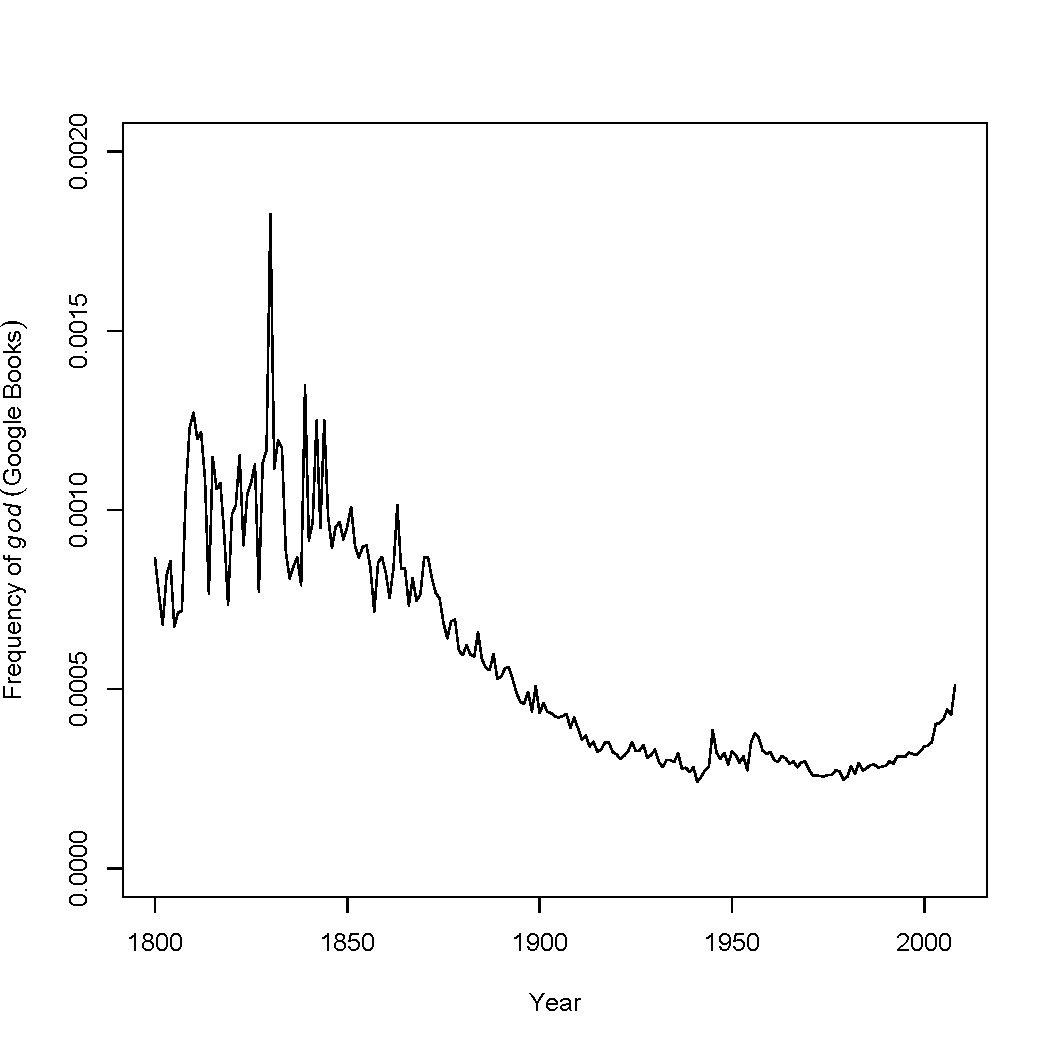
\includegraphics[width=\textwidth]{figures/demiseofgodgoogle}
\end{minipage}
%
\begin{minipage}{.5\textwidth}
 \centering
 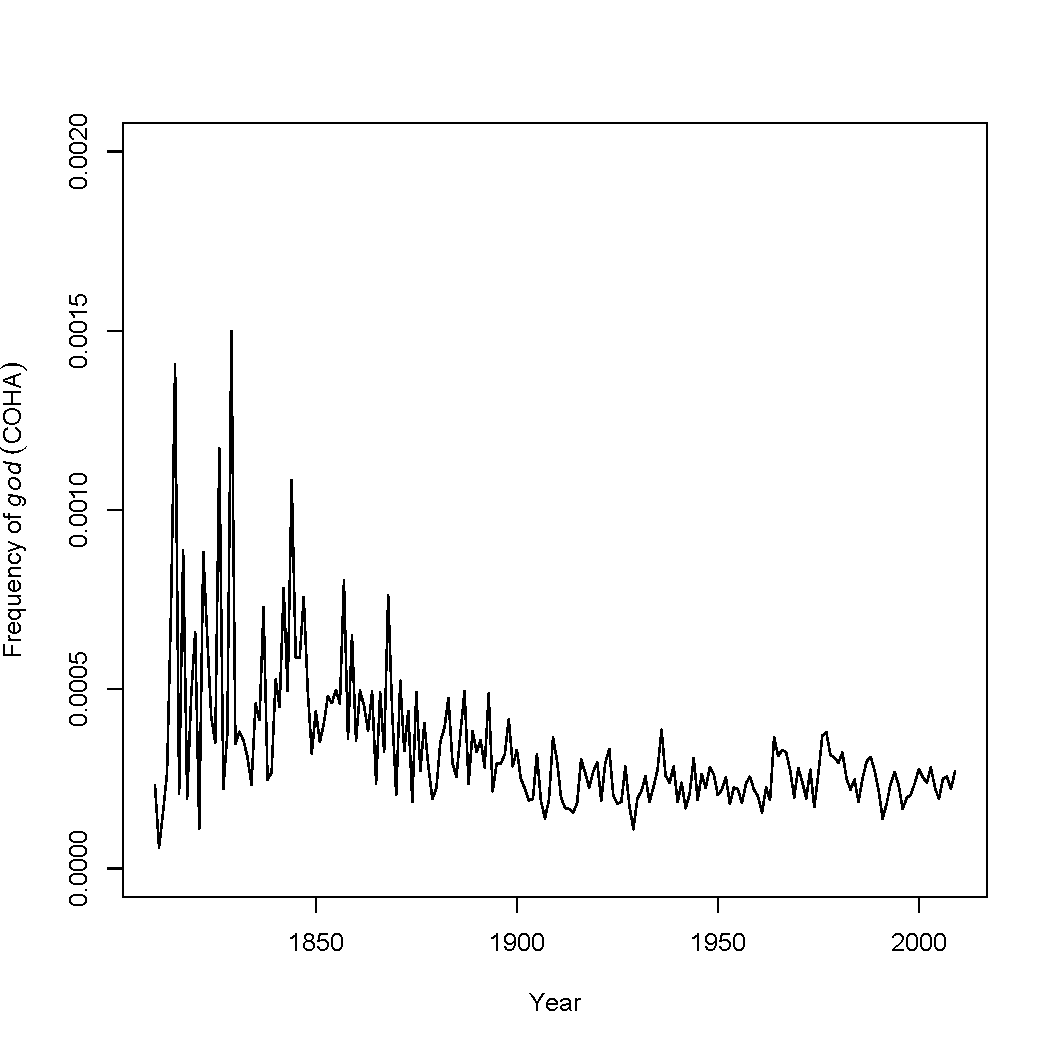
\includegraphics[width=\textwidth]{figures/demiseofgodcoha}
\end{minipage}
\end{figure}
%layout: why do these not render next to each other?

Clearly, the word \textit{God} has decreased in frequency \is{frequency} -- dramatically so in the Google Books archive, slightly less dramatically so in COHA. \is{COHA} The question is what conclusions to draw from this. The authors present it as an example of the ``history of religion'', concluding from their result somewhat flippantly that ```God' is not dead but needs a new publicist''. This flippancy, incidentally, signals an unwillingness to engage with their own results in any depth that is not entirely untypical of researchers in ``culturomics''. \is{culturomics}

Broadly speaking the result certainly suggests a waning dominance of religion on topic selection in book publishing (Google Books), and slightly less so in published texts in general (COHA). \is{COHA} This is not surprising to anyone who has paid attention for the last 200 years; more generally, it is not surprising that the rise and fall in importance of particular topics is reflected in the frequency \is{frequency} of the vocabulary used to talk and write about these topics, but the point of this case study was mainly to demonstrate that the method works.

While it is not implausible to analyze culture \is{culture} in general on the basis of a literary \is{literary language} corpus, any analysis that involves the area of publishing itself will be particularly convincing. One such example is the use of frequencies \is{frequency} to identify periods of censorship in \citet{michel_quantitative_2011}. For example, they search for the name of the Jewish artist \textit{Marc Chagall} in the German and the US\hyp{}English corpora. As Figure \ref{fig:marcchagall} shows, there is a first peak in the German corpus around 1920, but during the time of the Nazi government, the name drops to almost zero while it continues to rise in the US\hyp{}English corpus.

\begin{figure}[!htbp]
\caption{The name \textit{Marc Chagall} in the US\hyp{}English and the German parts of the Google Books corpus}
\label{fig:marcchagall}
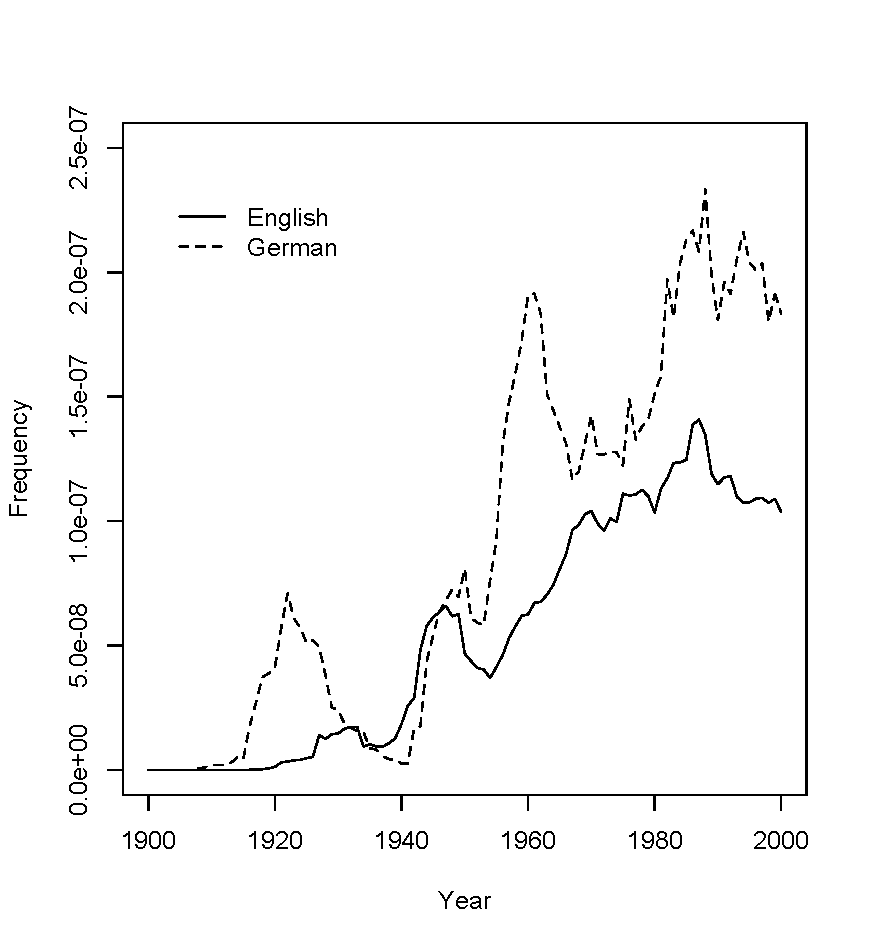
\includegraphics[width=.8\textwidth,keepaspectratio]{figures/chagallcensored}
\end{figure}

The authors plausibly take this drastic drop in frequency \is{frequency} as evidence of political censorship -- Chagall's works, like those of other Jewish artists, were declared to be ``degenerate'' and confiscated from museums, and it makes sense that his name would not be mentioned in books written in Nazi Germany. However, the question is, again, what conclusions to draw from such an analysis. Specifically, we know how to interpret the drop in frequency \is{frequency} of the name \textit{Marc Chagall} during the Nazi era in Germany because we know that Marc Chagall's works were banned. But if we did not know this, we would not know how to interpret the change in frequency, since words, especially names, may rise or fall in frequency for all kinds of reasons.

Consider the following figure, which shows the development of the frequency \is{frequency} of the name \textit{Karl Marx} in the German and English Google Books archive (extracted from the bigram \is{bigram} files downloaded from the Google Books site, see Supplementary Online Material, file CUBF). Note the different frequency scales -- the name is generally much more frequent in German than in English, but what interests us are changes in frequency.

\begin{figure}[!htbp]
\caption{The name \textit{Karl Marx} in the English and the German parts of the Google Books corpus}
\label{fig:karlmarx}
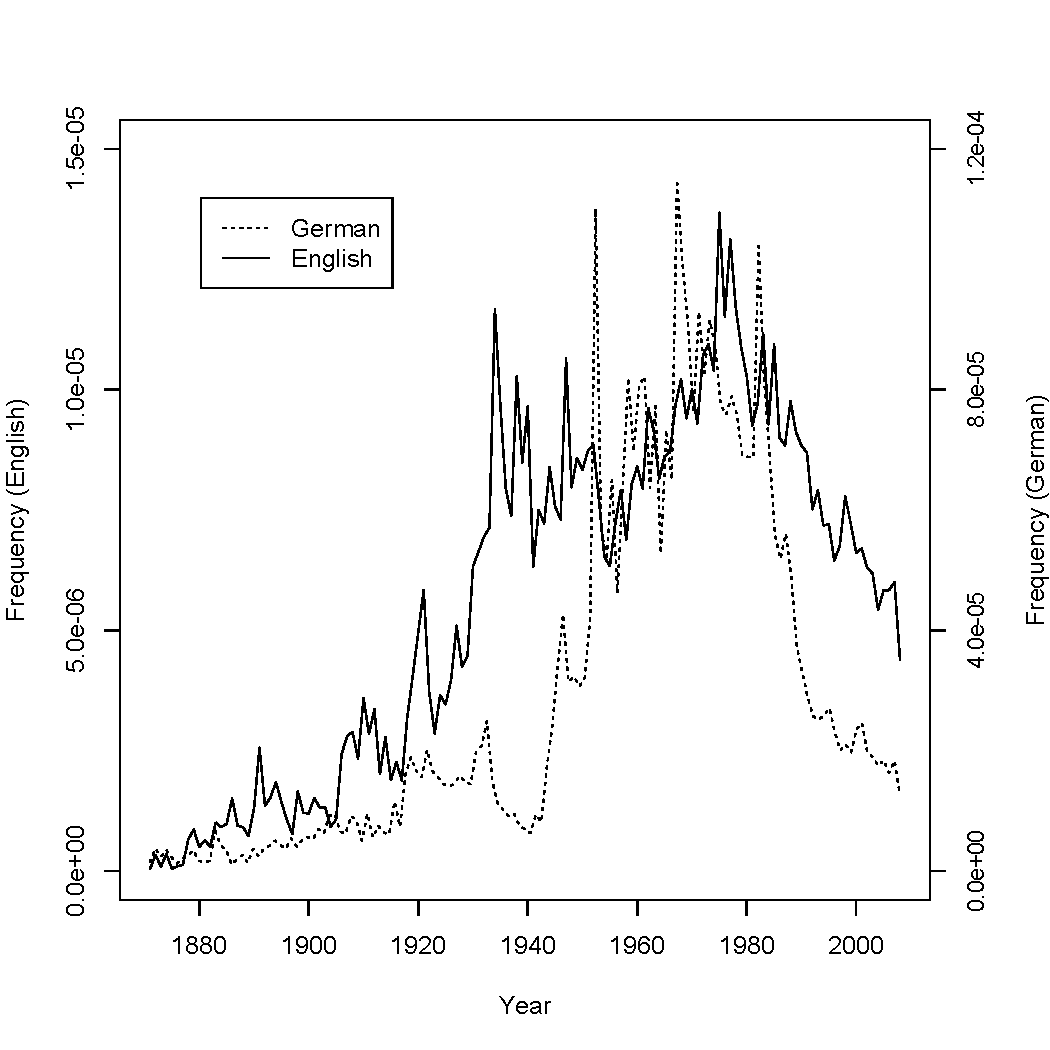
\includegraphics[width=.8\textwidth,keepaspectratio]{figures/karlmarx}
\end{figure}

Again, we see a rise in frequency \is{frequency} in the 1920s, and then a visible decrease during the Nazi era from 1933 to 1945. Again, this can plausibly be seen as evidence for censorship in Nazi Germany. Plausibly, because we know that the Nazis censored Karl Marx's writings -- they were among the first books to be burned in the Nazi book burnings of 1933. But what about other drops in frequency, both in English and in German? There are some noticeable drops in frequency in English: after 1920, between 1930 and 1940 (with some ups and downs), and at the beginning of the 1950s. Only the latter could plausibly be explained as the result of (implicit) censorship during the McCarthy era. Finally, the frequency \is{frequency} drops massively in both languages after 1980, but there was no censorship in either speech community. A more plausible explanation \is{explanation} is that in the 1980s, neoliberal capitalism became a very dominant ideology, \is{ideology} and Marx's communist ideas simply ceased to be of interest to many people (if this explanation is correct, we might see the frequency of the name rise again, given the current wide\hyp{}spread disillusionment with neoliberalism).

Thus, the rise and fall in frequency \is{frequency} cannot be attributed to a particular cause without an investigation of the social, economic and political developments during the relevant period. As such, ``culturomics'' \is{culturomics} can at best point us towards potentially interesting cultural changes that then need to be investigated in other disciplines. At worst, it will simply tell us what we already know from those other disciplines. In order to unfold their potential, such analyses would have to be done at a much larger scale -- the technology and the resources are there, and with the rising interest in ``digital humanities'' \is{humanities} we might see such large\hyp{}scale analyses at some point.

\chapter{Metaphor}
\label{ch:metaphorandmetonymy}

The ease with which corpora are accessed via word forms is an advantage as long as it is our aim to investigate words, for example with respect to their relationship to other words, to their internal structure or to their distribution \is{distribution, conditional} across grammatical \is{grammar} structures and across texts and language varieties. \is{language variety} As we saw in Chapter \ref{ch:grammar}, the difficulty of accessing corpora at levels of linguistic representation other than the word form is problematic where our aim is to investigate grammar in its own right, but since grammatical structures tend to be associated \is{association} with particular words and\slash or morphemes, \is{morphology} these difficulties can be overcome to some extent.

When it comes to investigating phenomena that are not lexical in nature, the word\hyp{}based nature of corpora is clearly a disadvantage and it may seem as though there is no alternative to a careful manual \is{manual analysis} search and\slash or a sophisticated annotation \is{annotation} (manual, semi\hyp{}manual or based on advanced natural\hyp{}language technology). However, corpus linguists have actually uncovered a number of relationships between words and linguistic phenomena beyond lexicon \is{lexicon} and grammar \is{grammar} without making use of such annotations. \is{annotation} In the final chapter of this book, we will discuss a number of case studies of one such phenomenon: metaphor. \is{figurative language} \is{metaphor}

\section{Studying metaphor in corpora}
\label{sec:studyingmetaphorincorpora}

Metaphor \is{figurative language} \is{metaphor} is traditionally defined as the transfer of a word from one referent (variously called vehicle, figure or source) to another (the tenor, ground or target) (cf. e.g. Aristotle, \textit{Poetics}, XXI). If metaphor were indeed located at the word level, it should be straightforwardly amenable to corpus\hyp{}linguistic analysis. Unfortunately, things are slightly more complicated. First, the transfer does not typically concern individual words but entire semantic \is{semantics} fields (or even conceptual \is{cognitive linguistics} domains, according to some theories). Second, as discussed in some detail in Chapter \ref{ch:retrievalannotation}, there is nothing in the word itself that distinguishes its literal \is{literalness} and metaphorical uses. One way around this problem is manual \is{manual analysis} annotation, \is{annotation} and there are very detailed and sophisticated proposals for annotation procedures (most notably the Pragglejaz Metaphor Identification Procedure, cf., for example, \citet{low_pragglejaz_2010}).

However, as stressed in various places throughout this book, the manual \is{manual analysis} annotation \is{annotation} of corpora severely limits the amount of data that can be included in a research design; \is{research design} this does not invalidate manual annotation, but it makes alternatives highly desirable. Two broad alternatives have been proposed in corpus linguistics. Since these were discussed in some detail in Chapter \ref{ch:retrievalannotation}, we will only repeat them briefly here before illustrating them in more detail in the case studies.

\section{Case studies}
\label{sec:metaphorcasestudies}

The first approach to extracting \is{retrieval} metaphors \is{figurative language} \is{metaphor} from corpora starts from a source domain, searching for individual words or sets of words (synonym \is{synonymy} sets, semantic \is{semantics} fields, discourse domains) and then identifying the metaphorical uses and the respective targets and underlying metaphors manually. \is{manual analysis} This approach is extensively demonstrated, for example, in \citet{deignan_corpus-based_1999, deignan_metaphorical_1999, deignan_metaphor_2005}. The three case studies in Section \ref{sec:sourcedomains} use this approach. The second approach starts from a target domain, searching for abstract words describing (parts of) the target domain and then identifying those that occur in a grammatical \is{grammar} pattern together with items from a different semantic \is{semantics} domain (which will normally be a source domain). This approach has been taken by \citet{stefanowitsch_happiness_2004, stefanowitsch_words_2006} and others. The case studies in Section \ref{sec:targetdomains} use this approach. A third approach has been suggested by \citet{wallington_metaphoricity_2003}: they attempt to identify words that are not themselves part of a metaphorical \is{figurative language} \is{metaphor} transfer but that point to a metaphorical transfer in the immediate context (the expression \textit{figuratively speaking} would be an obvious candidate). This approach has not been taken up widely, but it is very promising at least for the identification of certain types of metaphor, and of course the expressions in question are worthy of study in their own right, so one of the case studies in Section \ref{sec:metaphorandtext} takes a closer look at it.

\subsection{Source domains}
\label{sec:sourcedomains}

Among other things, the corpus\hyp{}based study of (small set of) source domain words may provide insights into the systematicity of metaphor \is{figurative language} \is{metaphor} \citep[cf. esp.][]{deignan_metaphorical_1999}. In cognitive \is{cognitive linguistics} linguistics, it is claimed that metaphor is fundamentally a mapping from one conceptual \is{cognitive linguistics} domain to another, and that metaphorical expressions are essentially a reflex of such mappings. This suggests a high degree of isomorphism between literal \is{literalness} and metaphorical \is{figurative language} \is{metaphor} language: words should essentially display the same systemic and usage\hyp{}based behavior when they are used as the source domain of a metaphor as when they are used in their literal sense unless there is a specific reason in the semantics \is{semantics} of the target domain that precludes this \citep{lakoff_contemporary_1993}.

\subsubsection{Case study: Lexical relations and metaphorical mapping}
\label{sec:antonymymetaphor}

\citet{deignan_metaphorical_1999} tests the isomorphism between literal \is{literalness} and metaphorical \is{figurative language} \is{metaphor} uses of source\hyp{}domain vocabulary very straightforwardly by looking at synonymy \is{synonymy} and antonymy. \is{antonymy} Deignan argues that these lexical relations should be transferred to the target domain, such that, for example, metaphorical meanings \is{semantics} of \textit{cold} and \textit{hot} should also be found for \textit{cool} and \textit{warm} respectively, since their literal meanings are very similar. Likewise, metaphorical \is{figurative language} \is{metaphor} \textit{hot} and \textit{cold} should encode opposites in the same way they do in their literal \is{literalness} uses.

Let us replicate \is{replicability} Deignans study using the BNC Baby. \is{BNC Baby} To keep other factors equal, let us focus on attributive uses of adjectives \is{adjective} that modify target domain nouns \is{noun} (as in \textit{cold facts}), or nouns that are themselves used metaphorically (as in ``The project went into \textit{cold storage}'' meaning work on it ceased). Deignan focuses on the base forms of these adjectives, \is{adjective} let us do the same. She also excludes ``highly fixed collocations \is{collocation} and idioms'' \is{idiomaticity} because their potential metaphorical \is{figurative language} \is{metaphor} origin may no longer be transparent -- let us not follow her here, as we can always identify and discuss such cases after we have extracted \is{retrieval} and tabulated our data.

Deignan does not explicitly present an annotation \is{annotation} scheme, but she presents dictionary\hyp{}like \is{dictionary} definitions of her categories and extensive examples of her categorization \is{categorization} decisions that, taken together, serve the same function. Her categories differ in number (between four and ten) and semantic \is{semantics} granularity across the four words, let us design \is{research design} a stricter annotation \is{annotation} scheme with a minimal number of categories. \is{categorization}

Let us assume that survey of the dictionaries \is{dictionary} already used in Case Study \ref{sec:semanticdifferencesbetweenicandical} yields the following major metaphor \is{figurative language} \is{metaphor} categories:

\begin{enumerate}

\item \textvv{activity}, with the metaphors \textsc{high activity is heat} and \textsc{low activity is coldness}, as in \textit{cold\slash hot war}, \textit{hot pursuit}, \textit{hot topic}, etc.). This sense is not recognized by the dictionaries, \is{dictionary} except insofar as it is implicit in the definitions of \textit{cold war}, \textit{hot pursuit}, \textit{cold trail}, etc. It is understood here to include a sense of \textit{hot} described in dictionaries as ``currently popular'' or ``of immediate interest'' (e.g. \textit{hot topic}).

\item \textvv{affection}, with the metaphors \is{figurative language} \is{metaphor} \textsc{affection is heat} and \textsc{indifference is coldness}, as in \textit{cold stare}, \textit{warm welcome}, etc. This sense is recognized by all dictionaries, \is{dictionary} but we will interpret it to include sense connected with sexual attraction and (un)responsiveness, e.g. \textit{hot date}.

\item \textvv{temperament}, with the metaphors \is{figurative language} \is{metaphor} \textsc{emotional behavior is heat} and \textsc{rational behavior is coldness}, as in \textit{cool head}, \textit{cold facts}, \textit{hot temper}, etc. Most dictionaries \is{dictionary} recognize this sense as distinct from the previous one -- both are concerned with emotion \is{emotions} or its absence, but in case of the \textvv{affection}, the distinction is one between affectionate feelings and their absense, in the case of \textvv{temperament} the distinction is one between behavior based on any emotion \is{emotions} and behavior unaffected by emotion.

\item \textsc{synesthesia}, a category covering uses described in dictionaries \is{dictionary} as ``conveying or producing the impression of being hot, cold, etc.'' in some sensory domain other than temperature, i.e. \textit{warm color}, \textit{cold light}, \textit{cool voice}, etc.

\item \textsc{evaluation}, with the (potential) metaphor \textsc{positive things have a temperature}, as in \textit{a really cool movie}, \textit{a cool person}, \textit{a hot new idea}, etc. This may not be a metaphor \is{figurative language} \is{metaphor} at all, as both uses are very idiomatic; \is{idiomaticity} in fact, \textit{hot} in this sense could be included under \textit{activity} or \textit{affection}, and \textit{cool} in this sense is presumably derived from \textit{temperament}.

\end{enumerate}

Table \ref{tab:temperaturemetaphors} lists the token \is{token (instance)} frequencies \is{frequency, token} of the four adjectives \is{adjective} with each of these broad metaphorical \is{figurative language} \is{metaphor} categories as well as all types \is{type (category)} instantiating the respective category. There is one category that does not show any significant deviations from the expected \is{frequency, expected} frequencies, namely the infrequently instantiated category \textvv{synesthesia}. For all other categories, there are clear differences that are unexpected from the perspective of conceptual \is{cognitive linguistics} metaphor theory.

\begin{sidewaystable}[!htbp]
\caption{\textsc{temperature} metaphors (BNC Baby)}
\label{tab:temperaturemetaphors}
\resizebox{0.9\textwidth}{!}{%
\begin{tabular}[t]{lccccr}
\lsptoprule
 & \multicolumn{4}{c}{\textvv{Adjective}} & \\
\textvv{Noun} & \textvv{cold} & \textvv{cool} & \textvv{warm} & \textvv{hot} & Total \\
\midrule
\textvv{\makecell[tl]{activity}}
% me: cold-activity
	& \makecell[t]{\begin{tabular}[t]{lS[table-format=2.2]}
		\small{\textit{Obs.:}} & 13 \\
		\small{\textit{Exp.:}} & 8.36 \\
		\small{\textit{$\chi^2$:}} & 2.57531100478469 \\
		\multicolumn{2}{l}{
			\begin{minipage}[t]{0.2\textwidth} \raggedright
			\footnotesize{\textit{storage}, \textit{turkey}, \textit{war}}
		\end{minipage}}
		\end{tabular}}
% me: cool-activity
	& \makecell[t]{\begin{tabular}[t]{lS[table-format=2.2]}
		\small{\textit{Obs.:}} & 0 \\
		\small{\textit{Exp.:}} & 4.62 \\
		\small{\textit{$\chi^2$:}} & 4.62 \\
		\multicolumn{2}{l}{
			\begin{minipage}[t]{0.2\textwidth} \raggedright
			\footnotesize{--}
		\end{minipage}}
		\end{tabular}}
% me: warm-activity
	& \makecell[t]{\begin{tabular}[t]{lS[table-format=2.2]}
		\small{\textit{Obs.:}} & 0 \\
		\small{\textit{Exp.:}} & 3.96 \\
		\small{\textit{$\chi^2$:}} & 3.96 \\
		\multicolumn{2}{l}{
			\begin{minipage}[t]{0.2\textwidth} \raggedright
			\footnotesize{--}
		\end{minipage}}
		\end{tabular}}
% me: hot-activity
	& \makecell[t]{\begin{tabular}[t]{lS[table-format=2.2]}
		\small{\textit{Obs.:}} & 9 \\
		\small{\textit{Exp.:}} & 5.06 \\
		\small{\textit{$\chi^2$:}} & 3.06790513833992 \\
		\multicolumn{2}{l}{
			\begin{minipage}[t]{0.2\textwidth} \raggedright
			\footnotesize{\textit{pursuit}, \textit{seat}, \textit{spot}, \textit{time}, \textit{war}}
		\end{minipage}}
		\end{tabular}}
	& 22 \\[1.6cm]
\textvv{\makecell[tl]{affection}}
% me: cold-affection
	& \makecell[t]{\begin{tabular}[t]{lS[table-format=2.2]}
		\small{\textit{Obs.:}} & 9 \\
		\small{\textit{Exp.:}} & 10.26 \\
		\small{\textit{$\chi^2$:}} & 0.154736842105263 \\
		\multicolumn{2}{l}{
			\begin{minipage}[t]{0.2\textwidth} \raggedright
			\footnotesize{\textit{atmosphere}, \textit{disapproval}, \textit{eyes}, \textit{note}, \textit{person}, \textit{response}, \textit{sarcasm}, \textit{savagery}, \textit{shoulder}}
		\end{minipage}}
		\end{tabular}}
% me: cool-affection
	& \makecell[t]{\begin{tabular}[t]{lS[table-format=2.2]}
		\small{\textit{Obs.:}} & 0 \\
		\small{\textit{Exp.:}} & 5.67 \\
		\small{\textit{$\chi^2$:}} & 5.67 \\
		\multicolumn{2}{l}{
			\begin{minipage}[t]{0.2\textwidth} \raggedright
			\footnotesize{--}
		\end{minipage}}
		\end{tabular}}
% me: warm-affection
	& \makecell[t]{\begin{tabular}[t]{lS[table-format=2.2]}
		\small{\textit{Obs.:}} & 16 \\
		\small{\textit{Exp.:}} & 4.86 \\
		\small{\textit{$\chi^2$:}} & 25.5348971193416 \\
		\multicolumn{2}{l}{
			\begin{minipage}[t]{0.2\textwidth} \raggedright
			\footnotesize{\textit{affinities}, \textit{approval}, \textit{embrace}, \textit{feeling}, \textit{glow}, \textit{kiss}, \textit{liking}, \textit{nest}, \textit{presence}, \textit{relief}, \textit{smile}, \textit{welcome}}
		\end{minipage}}
		\end{tabular}}
% me: hot-affection
	& \makecell[t]{\begin{tabular}[t]{lS[table-format=2.2]}
		\small{\textit{Obs.:}} & 2 \\
		\small{\textit{Exp.:}} & 6.21 \\
		\small{\textit{$\chi^2$:}} & 2.85412238325282 \\
		\multicolumn{2}{l}{
			\begin{minipage}[t]{0.2\textwidth} \raggedright
			\footnotesize{\textit{date}, \textit{pants}}
		\end{minipage}}
		\end{tabular}}
	& 27 \\[2.7cm]
\textvv{\makecell[tl]{temperament}}
% me: cold-temperament
	& \makecell[t]{\begin{tabular}[t]{lS[table-format=2.2]}
		\small{\textit{Obs.:}} & 14 \\
		\small{\textit{Exp.:}} & 10.64 \\
		\small{\textit{$\chi^2$:}} & 1.06105263157895 \\
		\multicolumn{2}{l}{
			\begin{minipage}[t]{0.2\textwidth} \raggedright
			\footnotesize{\textit{approach}, \textit{blood}, \textit{calculation}, \textit{clarity}, \textit{facts}, \textit{reality}, \textit{reminder}}
		\end{minipage}}
		\end{tabular}}
% me: cool-temperament
	& \makecell[t]{\begin{tabular}[t]{lS[table-format=2.2]}
		\small{\textit{Obs.:}} & 13 \\
		\small{\textit{Exp.:}} & 5.88 \\
		\small{\textit{$\chi^2$:}} & 8.62149659863946 \\
		\multicolumn{2}{l}{
			\begin{minipage}[t]{0.2\textwidth} \raggedright
			\footnotesize{\textit{analysis}, \textit{composure}, \textit{customer}, \textit{firmness}, \textit{head}, \textit{look}, \textit{response}, \textit{restraint}, \textit{Rose (prop. name)}, \textit{silence}, \textit{temper}}
		\end{minipage}}
		\end{tabular}}
% me: warm-temperament
	& \makecell[t]{\begin{tabular}[t]{lS[table-format=2.2]}
		\small{\textit{Obs.:}} & 0 \\
		\small{\textit{Exp.:}} & 5.04 \\
		\small{\textit{$\chi^2$:}} & 5.04 \\
		\multicolumn{2}{l}{
			\begin{minipage}[t]{0.2\textwidth} \raggedright
			\footnotesize{--}
		\end{minipage}}
		\end{tabular}}
% me: hot-temperament
	& \makecell[t]{\begin{tabular}[t]{lS[table-format=2.2]}
		\small{\textit{Obs.:}} & 1 \\
		\small{\textit{Exp.:}} & 6.44 \\
		\small{\textit{$\chi^2$:}} & 4.59527950310559 \\
		\multicolumn{2}{l}{
			\begin{minipage}[t]{0.2\textwidth} \raggedright
			\footnotesize{\textit{spirits}}
		\end{minipage}}
		\end{tabular}}
	& 28 \\[2.7cm]
\textvv{\makecell[tl]{synesthesia}}
% me: cold-synesthesia
	& \makecell[t]{\begin{tabular}[t]{lS[table-format=2.2]}
		\small{\textit{Obs.:}} & 2 \\
		\small{\textit{Exp.:}} & 1.9 \\
		\small{\textit{$\chi^2$:}} & 0.005263157894737 \\
		\multicolumn{2}{l}{
			\begin{minipage}[t]{0.2\textwidth} \raggedright
			\footnotesize{\textit{fire}, \textit{grey}}
		\end{minipage}}
		\end{tabular}}
% me: cool-synesthesia
	& \makecell[t]{\begin{tabular}[t]{lS[table-format=2.2]}
		\small{\textit{Obs.:}} & 1 \\
		\small{\textit{Exp.:}} & 1.05 \\
		\small{\textit{$\chi^2$:}} & 0.002380952380952 \\
		\multicolumn{2}{l}{
			\begin{minipage}[t]{0.2\textwidth} \raggedright
			\footnotesize{\textit{voice}}
		\end{minipage}}
		\end{tabular}}
% me: warm-synesthesia
	& \makecell[t]{\begin{tabular}[t]{lS[table-format=2.2]}
		\small{\textit{Obs.:}} & 2 \\
		\small{\textit{Exp.:}} & 0.9 \\
		\small{\textit{$\chi^2$:}} & 1.34444444444444 \\
		\multicolumn{2}{l}{
			\begin{minipage}[t]{0.2\textwidth} \raggedright
			\footnotesize{\textit{colour}, \textit{glow}}
		\end{minipage}}
		\end{tabular}}
% me: hot-synesthesia
	& \makecell[t]{\begin{tabular}[t]{lS[table-format=2.2]}
		\small{\textit{Obs.:}} & 0 \\
		\small{\textit{Exp.:}} & 1.15 \\
		\small{\textit{$\chi^2$:}} & 1.15 \\
		\multicolumn{2}{l}{
			\begin{minipage}[t]{0.2\textwidth} \raggedright
			\footnotesize{--}
		\end{minipage}}
		\end{tabular}}
	& 5 \\[1.6cm]
\textvv{\makecell[tl]{evaluation}}
% me: cold-evaluation
	& \makecell[t]{\begin{tabular}[t]{lS[table-format=2.2]}
		\small{\textit{Obs.:}} & 0 \\
		\small{\textit{Exp.:}} & 6.84 \\
		\small{\textit{$\chi^2$:}} & 6.84 \\
		\multicolumn{2}{l}{
			\begin{minipage}[t]{0.2\textwidth} \raggedright
			\footnotesize{--}
		\end{minipage}}
		\end{tabular}}
% me: cool-evaluation
	& \makecell[t]{\begin{tabular}[t]{lS[table-format=2.2]}
		\small{\textit{Obs.:}} & 7 \\
		\small{\textit{Exp.:}} & 3.78 \\
		\small{\textit{$\chi^2$:}} & 2.74296296296296 \\
		\multicolumn{2}{l}{
			\begin{minipage}[t]{0.2\textwidth} \raggedright
			\footnotesize{\textit{countess}, \textit{dude}, \textit{million}, \textit{thing}}
		\end{minipage}}
		\end{tabular}}
% me: warm-evaluation
	& \makecell[t]{\begin{tabular}[t]{lS[table-format=2.2]}
		\small{\textit{Obs.:}} & 0 \\
		\small{\textit{Exp.:}} & 3.24 \\
		\small{\textit{$\chi^2$:}} & 3.24 \\
		\multicolumn{2}{l}{
			\begin{minipage}[t]{0.2\textwidth} \raggedright
			\footnotesize{--}
		\end{minipage}}
		\end{tabular}}
% me: hot-evaluation
	& \makecell[t]{\begin{tabular}[t]{lS[table-format=2.2]}
		\small{\textit{Obs.:}} & 11 \\
		\small{\textit{Exp.:}} & 4.14 \\
		\small{\textit{$\chi^2$:}} & 11.3670531400966 \\
		\multicolumn{2}{l}{
			\begin{minipage}[t]{0.2\textwidth} \raggedright
			\footnotesize{\textit{favourite}, \textit{gunner}, \textit{handicap}, \textit{multimedia system}, \textit{shot}, \textit{stuff}, \textit{tips}}
		\end{minipage}}
		\end{tabular}}
	& 18 \\[1.6cm]
\midrule
Total
	& \makecell[t]{38}
	& \makecell[t]{21}
	& \makecell[t]{23}
	& \makecell[t]{18}
	& \makecell[t]{100} \\
\lspbottomrule
\multicolumn{6}{l}{\scriptsize{Supplementary Online Material: WLVF}} \\ %OSM
\end{tabular}}
\end{sidewaystable}

The category \textit{activity} is instantiated only for the words \textit{cold} and \textit{hot} and its absence for the other two words is significant. We can imagine (and, in a sufficiently large \is{corpus size} data set, find) uses for \textit{cool} and \textit{warm} that would fall into this category. For example, Frederick Pohl's 1981 novel \emph{The Cool War} describes a geopolitical situation in which political allies sabotage each other's economies, and it is occasionally used to refer to real\hyp{}life situations as well. But this seems to be a deliberate analogy rather than a systematic use, leaving us with an unexpected gap in the middle of the linguistic scale between hot and cold.

The category \textit{affection} is found with three of the four words, but its absence for the word \textit{cool} is statistically significant, as is its clear overrepresentation with \textit{warm}. This lack of systematicity is even more unexpected than the one observed with \textit{activity}: for the latter, we could argue that it reflects a binary distinction that uses only the extremes of the scale, for example because there is not enough of a potential conceptual difference between a \textit{cold war} and a \textit{cool war}. With \textvv{affection}, in contrast, this explanation is not adequate, as the entire scale is used. It remains unclear, therefore, why \textit{warm} should be so prominently used here, and why \textit{cool} is so rare (it is possible: the dictionaries \is{dictionary} list examples like \textit{a cool manner}, \textit{a cool reply}).

With \textit{temperament}, we find a partially complementary situation: again, three of the four words occur with this metaphor, \is{figurative language} \is{metaphor} including, again, the extreme points. However, in this case it is \textit{cool} that is significantly overrepresented and \textit{warm} that is significantly absent. A possible explanation would be that there is a potential for confusion between the metaphors \textit{affection is temperature} and \textit{temperament is temperature}, and so speakers divide up the continuum from cold to hot between them. However, this does not explain why \textit{cold} is frequently used in both metaphorical senses.

The gaps in the last category, \textvv{evaluation}, are less confusing. As mentioned above, this is probably not a single coherent category and we would not expect uses to be equally disributed across the four words.

This case study demonstrates the use of corpus data to evaluate claims about conceptual structure. Specifically, it shows how a central claim of conceptual metaphor \is{figurative language} \is{metaphor} theory can be investigated (see the much more detailed discussion in \citet{deignan_metaphorical_1999}.

\subsubsection{Case study: Word forms in metaphorical mappings}
\label{sec:flamevsflames}

Another area in which we might expect a large degree of isomorphism between literal \is{literalness} and metaphorical \is{figurative language} \is{metaphor} uses of a word is the quantitative and qualitative distribution \is{distribution, conditional} of word forms. In a highly intriguing study, \citet{stefanowitsch_grammar_2006} investigate the metaphors associated \is{association} with the source domain words \textit{flame} and \textit{flames} in terms of whether they occur in positively or negatively connoted \is{connotation} contexts.

Her study is generally deductive \is{deduction} in that she starts with an expectation (if not quite a full\hyp{}fledged hypothesis) that there are frequently differences between the singular \is{number} and the plural forms of a metaphorically \is{figurative language} \is{metaphor} used word with respect to connotation. \is{connotation}

A cursory look at a few relatively randomly \is{chance} selected examples appears to corroborate this expression. More precisely, it seems that the singular form \textit{flame} has positive connotations \is{connotation} more frequently than expected \is{frequency, expected} (cf. (\ref{ex:flamemet}), while the plural \is{number} form \textit{flames} has negative connotations \is{connotation} more frequently than expected (cf. (\ref{ex:flamesmet}):

\begin{exe}
\ex
\begin{xlist}
\label{ex:flamemet}
\ex $[$T$]$he flame of hope burns brightly here. (BNC AJD)
\ex Emilio Estevez, sitting on the sofa next to old flame Demi Moore... (BNC CH1)
\end{xlist}
\end{exe}

\begin{exe}
\ex
\begin{xlist}
\label{ex:flamesmet}
\ex ...the flames of civil war engulfed the central Yugoslav republic. (BNC AHX)
\ex The game was going OK and then it went up in flames. (BNC CBG)
\end{xlist}
\end{exe}

Deignan studies this potential difference systematically based on a sample of more than 1500 hits for \textit{flame/s} in the Bank of English (a proprietary, non\hyp{}accessible corpus owned by HarperCollins), from which she manually \is{manual analysis} extracts \is{retrieval} all 153 metaphorical uses. These are then categorized \is{categorization} according to their connotation. \is{connotation} Deignan's design \is{research design} thus has two nominal \is{nominal data} variables: \textsc{Word Form of Flame} (with the variables \textsc{singular} and \textsc{plural}) \is{number} and \textsc{Connotation of Metaphor} \is{figurative language} \is{metaphor} (with the values \textsc{positive} and \textsc{negative}. She does not provide an annotation \is{annotation} scheme for categorizing \is{categorization} the metaphorical expressions, but she provides a set of examples that are intuitively quite plausible. Table \ref{tab:flamemetposneg} shows her results ($\chi^2$ = 53.98, df = 1, p < 0.001). \is{chi-square test}

\begin{table}[!htbp]
\caption{Positive and negative metaphors with singular and plural forms of \textit{flame} \citep[117]{stefanowitsch_grammar_2006}}
\label{tab:flamemetposneg}
\begin{tabular}[t]{llccr}
\lsptoprule
 & & \multicolumn{2}{c}{\textvv{Word Form of Flame}} & \\
 & & \textvv{singular} & \textvv{plural} & Total \\
\midrule
\textvv{\makecell[lt]{Connotation}}
	& \textvv{positive}
		& \makecell[t]{\num{90}\\\small{(\num{70.78})}}
		& \makecell[t]{\num{24}\\\small{(\num{43.22})}}
		& \makecell[t]{\num{114}\\} \\
	& \textvv{negative}
		& \makecell[t]{\num{5}\\\small{(\num{24.22})}}
		& \makecell[t]{\num{34}\\\small{(\num{14.78})}}
		& \makecell[t]{\num{39}\\} \\
\midrule
	& Total
		& \makecell[t]{\num{95}}
		& \makecell[t]{\num{58}}
		& \makecell[t]{\num{153}} \\
\lspbottomrule
\end{tabular}
\end{table}
% me: chisq.test(matrix(c(90,5,24,34),ncol=2),corr=FALSE)

Clearly, metaphorical \is{figurative language} \is{metaphor} singular \textit{flame} is used in positive metaphorical contexts much more frequently than metaphorical plural \is{number} \textit{flames}. Deignan tentatively explains this in relation to the literal \is{literalness} uses of \textit{flame(s)}: a single flame is ``usually under control'', and it may ``be if use, as a candle or a burning match''. If there is more than one flame, we are essentially dealing with a fire -- ``flames are often undesired, out of control and very dangerous'' \citep[117]{stefanowitsch_grammar_2006}.

This explanation itself is of course a hypothesis about the literal \is{literalness} use of singular \is{number} and plural \textit{flame} that must be tested separately. Deignan does not provide such a test, so let us do it here. Let us select a sample of 20 hits each for literal uses the singular and plural of \textit{flame(s)} from the BNC \is{BNC} (as mentioned above, Deignan's corpus is not accessible, so we must hope that the BNC is roughly comparable). Figure \ref{fig:flameconc} shows the sample for singular \is{number} (lines 1--20) and plural (21--40).

\begin{figure}[!htbp]
\caption{Concordance of \textit{flame(s)} (BNC, Sample)}
\label{fig:flameconc}
\hrulefill
\begin{fitverb}
 1 ford base . The jet crashed in a ball of [flame] , destroying 15 cars and damaging 10 mo
 2  face down , applying the cheroot to the [flame] . But his eyes never left the four men
 3 ls of a child 's that had passed through [flame] and were partially melted . They would
 4 ontainer next to him . An orange ball of [flame] ripped up into the sky , bathing the de
 5 went out of one door but then a sheet of [flame] came down and blocked me , so I had to
 6  . The fire burns evenly with a thin hot [flame] , as though there are no oils or resins
 7 ill-smouldering logs , fanning them into [flame] . He places some more logs from a pile
 8  of sherry to the momentary blue veil of [flame] on the pudding , been what she would ha
 9 truck one and cupped his hand around the [flame] . ` Cheers , ' said the man and dis
10 ed with the element , burning circles of [flame] round creatures she had demanded Ariel
11 the soft promise of the light burst into [flame] ; the vanguard of the islanders fell ba
12 arched for his lighter , and touched the [flame] to the tip to make contact with him . I
13  again , tighter this time , guiding the [flame] . She sucked , and the cigarette end gl
14   There , ' she shouted , pluming liquid [flame] from one claw , ` you 're not the onl
15 and steady to bring the cigarette to the [flame] and kept it for a few seconds longer th
16 ern horns outside their house , the weak [flame] of the candles fluttering in their prot
17 the upstairs windows , a sudden spurt of [flame] , and a part of the roof begin to sag o
18  however , disappear in a white sheet of [flame] . He just kept right on kicking Pikey ,
19 ue to finish . Do n't cook over a fierce [flame] . The outside of the food will cook bef
20 no cushion . Candle erm Church , steeple [Flame] . Steeple . Got it got it got it got it
\hrulefill
21 it was winning its battle to put out the [flames] . He had to do it now , while it was s
22 ner , arm raised . Its back was to him , [flames] still glowing deep in its side . He ra
23  how the roof caved in before a sheet of [flames] spread across the fuselage , cutting h
24 control down a steep hill and burst into [flames] . The fully-laden truck careered throu
25 s spent more than two hours fighting the [flames] , police said . Bowbazaar , in the cen
26 h a shining chair by a fire with fragile [flames] . These images had what Alexander desi
27 lood rejected -- racks of fragile spiked [flames] of votive candles , elaborate china an
28 ce , looking into the authentic fake gas [flames] as he sipped his drink . He touched hi
29 ross to the fireplace , staring into the [flames] . ` There 's no reason why he should
30 the ground and died , no explosions , no [flames] reaching to the sky . It simply flippe
31 ack of her head , protected her from the [flames] and blocked out any further damage to
32 W went first , its roof torn open by the [flames] and blast as if by a giant unseen can
33 stunned and wearied by the water and the [flames] , the howling and frantic clangour of
34 annonballs , and caught the smell of the [flames] , of split flesh , and heard the howls
35  . And the best is yet to come . ' ` The [flames] of hell ? ' ` Exactly . Operatic
36 ds , then night crept back in around the [flames] . Trails of burning liquid spiderwebbe
37 e properly . Susan reeled away from us , [flames] springing up where she had been touche
38  , and his leg broke in two places . The [flames] were dying down . I could see his blac
39 mes and lower temperatures to reduce the [flames] . ` Eventually all the cooking was do
40 s . This is Crystal Palace going up in f [flames] . November the thirtieth nineteen thir
\end{fitverb}
\hrulefill
\end{figure}

It is difficult to determine which hits should be categorized \is{categorization} as positive and which as negative. Let us assume that any unwanted and\slash or destructive fire should be characterized as negative, and, on this basis, categorize lines 1, 3, 4, 5, 11, 14, 17, 18, 21, 22, 23, 24, 25, 30, 31, 33, 34, 35, 36, 37, 38 and 40 as \textvv{negative} and the rest as \textvv{positive}. This would give us the result in Table \ref{tab:flamelitposneg} (if you disagree with the categorization, \is{categorization} come up with your own and do the corresponding calculations).

\begin{table}[!htbp]
\caption{Positive and negative contexts for literal uses of singular and plural forms of \textit{flame/s}}
\label{tab:flamelitposneg}
\begin{tabular}[t]{llccr}
\lsptoprule
 & & \multicolumn{2}{c}{\textvv{Word Form of Flame}} & \\
 & & \textvv{positive} & \textvv{negative} & Total \\
\midrule
\textvv{\makecell[lt]{Connotation}}
	& \textvv{singular}
		& \makecell[t]{\num{12}\\\small{(\num{9.00})}}
		& \makecell[t]{\num{8}\\\small{(\num{11.00})}}
		& \makecell[t]{\num{20}\\} \\
	& \textvv{plural}
		& \makecell[t]{\num{6}\\\small{(\num{9.00})}}
		& \makecell[t]{\num{14}\\\small{(\num{11.00})}}
		& \makecell[t]{\num{20}\\} \\
\midrule
	& Total
		& \makecell[t]{\num{18}}
		& \makecell[t]{\num{22}}
		& \makecell[t]{\num{40}} \\
\lspbottomrule
\end{tabular}
\end{table}
% me: chisq.test(matrix(c(12,6,8,14),ncol=2),corr=FALSE)

It does seem that negative connotations \is{connotation} are found more frequently with literal \is{literalness} uses of the plural form \textit{flames} than with literal uses of the singular form \textit{flame}. Despite the small size \is{corpus size} of the sample used here, this difference only just fails to reach statistical significance ($\chi^2$ = 3.64, df = 1, p = 0.0565). The difference would likely become significant if we used a larger sample. However, it is nowhere near as pronounced as in the metaphorical \is{figurative language} \is{metaphor} uses presented by Deignan. A crucial difference between literal \is{literalness} and metaphorical uses may be that fire is inherently dangerous and so literal references to fire are more likely to be negative than metaphorical ones, that allow us to focus on other aspects of fire. Interestingly, however, most of the negative uses of singular \is{number} \textit{flame} occur in constructions like \textit{ball of flame}, \textit{sheet of flame} and \textit{spurt of flame}, where \textit{flame} could be argued to be a mass noun \is{noun} rather than a true singular form. If we remove these five uses, then the difference between singular and plural becomes very significant even in the now further reduced sample ($\chi^2$ = 8.58, df = 1, p < 0.01).

Thus, Deignan's explanation appears to be generally correct, providing evidence for a substantial degree of isomorphism between literal \is{literalness} and figurative \is{figurative language} uses of (at least some) words. An analysis of more such cases could show whether this isomorphism between literal and metaphorical \is{figurative language} \is{metaphor} uses is a general principle (as the conceptual \is{cognitive linguistics} theory of metaphor as \citet{lakoff_contemporary_1993} suggests it should be.

This case study demonstrates first, how to approach the study of metaphor starting from source\hyp{}domain words, and, second, that such an approach may be applied not just descriptively, \is{description} but in the context of answering fundamental questions about the nature of metaphor. \is{figurative language} \is{metaphor}

\subsubsection{Case study: The impact of metaphorical expressions}
\label{sec:theimpactofmetaphoricalexpressions}

A slightly different example of a source\hyp{}domain oriented study is found in \citet{stefanowitsch_function_2005}, which investigates the relationship between metaphorical and literal \is{literalness} expressions hinted at at the end of the preceding case study. The aim of the study is to uncover evidence for the function of metaphorical \is{figurative language} \is{metaphor} expressions that have literal paraphrases, such as [\textit{dawn of} NP] in examples like (\ref{ex:dawnof}a), which is seemingly equivalent to the literal \is{literalness} [\textit{beginning of} NP] in (\ref{ex:dawnof}b):

\begin{exe}
\ex
\begin{xlist}
\label{ex:dawnof}
\ex $[$I$]$t has taken until the dawn of the 21st century to realise that the best methods of utilising . . . our woodlands are those employed a millennium ago. (BNC AHD)
\ex Communal life survived until the beginning of the nineteenth century and traditions peculiar to that way of life had lingered into the present. (BNC AEA)
\end{xlist}
\end{exe}

Other examples studied in \citet{stefanowitsch_function_2005} are \textit{in the center\slash heart of}, \textit{at the center\slash heart of} and \textit{a(n) increase\slash growth\slash rise in}. The studies have two nominal \is{nominal data} variables: the independent variable is \textvv{Metaphoricity of Pattern} (whose values are pairs of patterns like the one illustrated in examples (\ref{ex:dawnof}a, b)), the dependent variable is \textvv{Noun} (whose values are the nouns in the NP slot provided by these patterns. Methodologically, this corresponds to a differential collexeme \is{collostructional analysis} \is{collexeme, differential} analysis (Chapter \ref{ch:grammar}, Case Study \ref{sec:ditransitiveandprepositionaldative}).

The studies are deductive \is{deduction} in that they aim to test the hypothesis that metaphorical \is{figurative language} \is{metaphor} language serves a cognitive \is{cognitive linguistics} function and that for each pair of patterns investigated, the metaphorical variant should be used with nouns \is{noun} referring to more complex entities. The construct \textsc{complexity} is operationalized \is{operationalization} in the form of axioms derived from gestalt psychology, \is{psychology} such as the following:

\begin{quote}
Concepts representing entities that have a simple shape and\slash or have a clear boundary are less complex than those representing entities with complex shapes or fuzzy boundaries (because they are more easily delineable). This follows from the gestalt principles of closure and simplicity \citep[170]{stefanowitsch_function_2005}.
\end{quote}

For each pair of expressions, the differential collexemes \is{collostructional analysis} \is{collexeme, differential} are identified and the resulting lists are compared against these axiomatic assumptions. Let us illustrate this using the pattern \textit{the dawn\slash beginning of NP}. A case insensitive query for the string \texttt{dawn} or \texttt{beginning}, followed by \textit{of}, followed by up to three words that are not a noun, \is{noun} followed by a noun yields the results shown in Table \ref{tab:dawnofdifferential} (they are very similar to those based on a more careful manual extraction \is{retrieval} in \citealt{stefanowitsch_function_2005}).

\begin{table}[!htbp]
\caption{Differential collexemes of \textit{beginning of NP} and \textit{dawn of NP} (BNC)}
\label{tab:dawnofdifferential}
\resizebox{\textwidth}{!}{%
\begin{tabular}[t]{l *{2}{S[table-format=4]} *{2}{S[table-format=8]} S}
\lsptoprule
\multicolumn{1}{c}{\makecell[tc]{\textvv{Collexeme}}} & \multicolumn{1}{c}{\makecell[tc]{Frequency \\ with \textvv{dawn}}} & \multicolumn{1}{c}{\makecell[tc]{Frequency \\ with \textvv{beginning}}} & \multicolumn{1}{c}{\makecell[tc]{Other words \\ with \textvv{dawn}}} & \multicolumn{1}{c}{\makecell[tc]{Other words \\ with \textvv{beginning}}} & \multicolumn{1}{c}{\makecell[tc]{G\textsuperscript{2}}} \\
\midrule
\multicolumn{6}{l}{Most strongly associated with \textvv{dawn}} \\
\midrule
\textit{civilisation} & 25 & 1 & 112 & 3584 & 161.385803778975 \\
\textit{history} & 9 & 12 & 128 & 3573 & 32.180697883425 \\
\textit{time} & 13 & 39 & 124 & 3546 & 31.2657527467307 \\
\textit{era} & 10 & 30 & 127 & 3555 & 23.872749059115 \\
\textit{dream} & 4 & 1 & 133 & 3584 & 21.598766197973 \\
\textit{mankind} & 3 & 0 & 134 & 3585 & 19.8759726284138 \\
\textit{day} & 9 & 33 & 128 & 3552 & 18.7007109334932 \\
\textit{age} & 5 & 8 & 132 & 3577 & 16.4543085057119 \\
\multicolumn{6}{l}{...} \\
\midrule
\multicolumn{6}{l}{Most strongly associated with \textvv{beginning}} \\
\midrule
\textit{year} & 1 & 317 & 136 & 3268 & 17.7844361675103 \\
\textit{century} & 4 & 382 & 133 & 3203 & 11.4120728157816 \\
\textit{chapter} & 0 & 100 & 137 & 3485 & 7.60512306421009 \\
\textit{end} & 0 & 94 & 137 & 3491 & 7.14281356737414 \\
\textit{war} & 0 & 75 & 137 & 3510 & 5.68395907143544 \\
\textit{week} & 0 & 61 & 137 & 3524 & 4.61396278618309 \\
\textit{month} & 0 & 60 & 137 & 3525 & 4.53769415111556 \\
\textit{period} & 0 & 55 & 137 & 3530 & 4.15666913330235 \\
\textit{term} & 0 & 51 & 137 & 3534 & 3.85223020091959 \\
\lspbottomrule
\end{tabular}}
\end{table}
% me: query: BNC; "dawn"%c "of"%c [pos!=".*NN.*"]{0,3} [pos=".*NN.*"]; and
% me: BNC; "beginning"%c "of"%c [pos!=".*NN.*"]{0,3} [pos=".*NN.*"];

Unsurprisingly, both expressions are associated \is{association} almost exclusively with words referring to events and time spans (or, in some cases, with entities that exist through time, like \textit{mankind}, or that we interact with through time, like \textit{chapter}). Crucially, most of the nouns \is{noun} associated with the literal \is{literalness} \textit{beginning of} refer to time spans with clear boundaries and a clearly defined duration (\textit{year}, \textit{century}, etc.), while those associated \is{association} with the metaphorical \is{figurative language} \is{metaphor} \textit{dawn of} refer to events and time spans without clear boundaries or a clear duration (\textit{civilization}, \textit{time}, \textit{history}, \textit{age}, \textit{era}, \textit{culture}). The one apparent exception is \textit{day}, but this occurs exclusively in literal \is{literalness} uses of \textit{dawn of}, such as \textit{It was the dawn of the fourth day since the murder} (BNC CAM). This (and similar results for other pairs of expressions) are presented in \citet{stefanowitsch_function_2005} as evidence for a cognitive \is{cognitive linguistics} function of metaphor. \is{figurative language} \is{metaphor}

In a short discussion of this study, \citet{liberman_what_2005} notes in passing that even individual decades and centuries may differ in the degree to which they prefer \textit{beginning of} or \textit{dawn of}: using internet search engines, he shows that \textit{dawn of the 1960s} is more probable than \textit{dawn of the 1980s} compared to \textit{beginning of the 1960s\slash 1980s}, and that \textit{dawn of the 21st century} is more probable than \textit{dawn of the 18th century} compared to \textit{beginning of the 18th\slash 21st century}. He rightly points out that this seems to call into question the properties of boundedness and well\hyp{}defined length that \citet{stefanowitsch_function_2005} appeals to, since obviously all decades\slash centuries are equally bounded.

Since search engine frequency data are notoriously unreliable, let us replicate \is{replicability} this observation in a large \is{corpus size} corpus, the 400+ million word Corpus of Contemporary American English (COCA). The names of decades (such as \textit{1960s} or \textit{sixties}) occur too infrequently with \textit{dawn of} in this corpus to say anything useful about them, but the names of centuries are frequent enough for a differential collexeme \is{collostructional analysis} \is{collexeme, differential} analysis.

Table \ref{tab:dawnofcentury} shows the percentage of \textit{dawn of} for the past ten centuries (spelling) variants of the respective centuries, such as \textit{19th century}, \textit{nineteenth century}, etc.) as well as spelling errors were normalized to the spelling shown in this table.

\begin{table}[!htbp]
\caption{Differential collexemes of \textit{dawn\slash beginning of \_\_ century} (COCA)}
\label{tab:dawnofcentury}
\resizebox{\textwidth}{!}{%
\begin{tabular}[t]{l *{2}{S[table-format=4]} *{2}{S[table-format=8]} S}
\lsptoprule
\multicolumn{1}{c}{\makecell[tc]{\textvv{Collexeme}}} & \multicolumn{1}{c}{\makecell[tc]{Frequency \\ with \textvv{dawn}}} & \multicolumn{1}{c}{\makecell[tc]{Frequency \\ with \textvv{beginning}}} & \multicolumn{1}{c}{\makecell[tc]{Other words \\ with \textvv{dawn}}} & \multicolumn{1}{c}{\makecell[tc]{Other words \\ with \textvv{beginning}}} & \multicolumn{1}{c}{\makecell[tc]{G\textsuperscript{2}}} \\
\midrule
\multicolumn{6}{l}{Most strongly associated with \textvv{dawn of \_\_ century}} \\
\midrule
\textit{the twenty-first} & 32 & 90 & 52 & 623 & 29.9285102625756 \\
\textit{a new} & 7 & 6 & 77 & 707 & 15.329855332433 \\
\textit{a} & 1 & 0 & 83 & 713 & 4.51077281590357 \\
\textit{America's} & 1 & 0 & 83 & 713 & 4.51077281590357 \\
\textit{an American} & 1 & 0 & 83 & 713 & 4.51077281590357 \\
\textit{an Asian} & 1 & 0 & 83 & 713 & 4.51077281590357 \\
\textit{our new} & 1 & 0 & 83 & 713 & 4.51077281590357 \\
\textit{that ancient} & 1 & 0 & 83 & 713 & 4.51077281590357 \\
\textit{the eleventh} & 1 & 0 & 83 & 713 & 4.51077281590357 \\
\textit{the incoming} & 1 & 0 & 83 & 713 & 4.51077281590357 \\
\midrule
\multicolumn{6}{l}{Most strongly associated with \textvv{beginning of \_\_ century}} \\
\midrule
\textit{the} & 2 & 94 & 82 & 619 & 11.4620118146882 \\
\textit{the nineteenth} & 2 & 68 & 82 & 645 & 6.39669989856688 \\
\textit{this} & 5 & 97 & 79 & 616 & 4.6940397471707 \\
\textit{the seventeenth} & 0 & 14 & 84 & 699 & 3.14778820208579 \\
\lspbottomrule
\end{tabular}}
\end{table}

There are clear differences between the centuries associated with \textvv{dawn} and those associated \is{association} with \textvv{beginning}: the literal \is{literalness} expression is associated with the past (\textit{nineteenth}, \textit{seventeenth} (just below significance)), while the metaphorical \is{figurative language} \is{metaphor} expression, as already observed by Liberman, is associated with the twenty\hyp{}first century, i.e., the future (the expressions \textit{a new}, \textit{our new} and \textit{the incoming} also support this). I would argue that this does point to a difference in boundedness and duration. While all centuries are objectively speaking, of the same length and have the same clear boundaries, it seems reasonable to assume that the past feels more bounded than the future because it is actually over, and we can imagine it in its entirety. In contrast, none of the speakers in the COCA will live to see the end of the 21st century, making it conceptually less bounded to them.

If this is true, then we should be able to observe the same effect in the past: When the twentieth century was still the future, it, too, should have been associated \is{association} with the metaphorical \is{figurative language} \is{metaphor} \textit{dawn of}. Let us test this hypothesis using the Corpus of Historical American English, which includes language from the early nineteenth to the very early twenty\hyp{}first century -- in a large part of the corpus, the twentieth century was thus entirely or partly in the future. Table \ref{tab:dawnofdifferentialcoha} shows the differential collexemes \is{collostructional analysis} \is{collexeme, differential} of the two expressions in this corpus.

\begin{table}[!htbp]
\caption{Differential collexemes of \textit{dawn\slash beginning of \_\_ century} (COHA)}
\label{tab:dawnofdifferentialcoha}
\resizebox{\textwidth}{!}{%
\begin{tabular}[t]{l *{2}{S[table-format=4]} *{2}{S[table-format=8]} S}
\lsptoprule
\multicolumn{1}{c}{\makecell[tc]{\textvv{Collexeme}}} & \multicolumn{1}{c}{\makecell[tc]{Frequency \\ with \textvv{dawn}}} & \multicolumn{1}{c}{\makecell[tc]{Frequency \\ with \textvv{beginning}}} & \multicolumn{1}{c}{\makecell[tc]{Other words \\ with \textvv{dawn}}} & \multicolumn{1}{c}{\makecell[tc]{Other words \\ with \textvv{beginning}}} & \multicolumn{1}{c}{\makecell[tc]{G\textsuperscript{2}}} \\
\midrule
\multicolumn{6}{l}{Most strongly associated with \textvv{dawn of \_\_ century}} \\
\midrule
\textit{the twenty\hyp{}first} & 7 & 14 & 23 & 908 & 24.0907472190799 \\
\textit{another} & 2 & 0 & 28 & 922 & 13.9616651831275 \\
\textit{america's} & 1 & 0 & 29 & 922 & 6.94739452091335 \\
\textit{that} & 1 & 0 & 29 & 922 & 6.94739452091335 \\
\textit{the twentieth} & 7 & 72 & 23 & 850 & 6.531541200179 \\
\midrule
\multicolumn{6}{l}{Most strongly associated with \textvv{beginning of \_\_ century}} \\
\midrule
\textit{this} & 0 & 108 & 30 & 814 & 7.34849897856036 \\
\lspbottomrule
\end{tabular}}
\end{table}

As predicted, the twentieth century is now associated \is{association} with the metaphorical \is{figurative language} \is{metaphor} expression (as is the twenty\hyp{}first). In addition, there is the expression \textit{America's century} in both corpora, and \textit{an American} and \textit{an Asian} in COCA. These, I would argue, do not refer to precise centuries but are to be understood as labels for eras. In sum, I would conclude that the idea of boundedness accounts for the apparent exceptions too, at least in the case of centuries, supporting a cognitive \is{cognitive linguistics} function of metaphor. \is{figurative language} \is{metaphor}

Even if we agree with this conclusion in general, however, it does not preclude a more literary, \is{literary language} rhetorical function for metaphor in addition: while some of the expression pairs investigated in \citet{stefanowitsch_function_2005} are fairly neutral with respect to genre \is{genre} or register, \is{register} metaphorical \is{figurative language} \is{metaphor} \textit{dawn of} intuitively has a distinctly literary flavor. To conclude this section, let us check the distribution \is{distribution, conditional} of the hits for the query outlined above across the text categories defined in the BNC. \is{BNC} Table \ref{tab:dawnbeginninggenre} shows the results (note that the categories Spoken Conversation \is{conversation} and Spoken Other from the BNC have been collapsed into a single category here).

\begin{table}[!htbp]
\caption{The expressions \textit{dawn of} and \textit{beginning of} by text category (BNC)}
\label{tab:dawnbeginninggenre}
\resizebox{0.6\textwidth}{!}{%
\begin{tabular}[t]{lccr}
\lsptoprule
 & \multicolumn{2}{c}{\textvv{Expression}} & \\
\textvv{Text Category} & \textvv{dawn of} & \textvv{beginning of} & Total \\
\midrule
\textvv{\makecell[tl]{prose}}
	& \makecell[t]{\begin{tabular}[t]{lS[table-format=2.2]} \small{\textit{Obs.:}} & 54 \\ \small{\textit{Exp.:}} & 50.72 \\ \small{\textit{$\chi^2$:}} & 0.21 \end{tabular}}
	& \makecell[t]{\begin{tabular}[t]{lS[table-format=2.2]} \small{\textit{Obs.:}} & 1324 \\ \small{\textit{Exp.:}} & 1327.28 \\ \small{\textit{$\chi^2$:}} & 0.01 \end{tabular}}
	& 1378 \\[1.1cm]
\textvv{\makecell[tl]{miscellaneous \\ published}}
	& \makecell[t]{\begin{tabular}[t]{lS[table-format=2.2]} \small{\textit{Obs.:}} & 30 \\ \small{\textit{Exp.:}} & 25.14 \\ \small{\textit{$\chi^2$:}} & 0.94 \end{tabular}}
	& \makecell[t]{\begin{tabular}[t]{lS[table-format=2.2]} \small{\textit{Obs.:}} & 653 \\ \small{\textit{Exp.:}} & 657.86 \\ \small{\textit{$\chi^2$:}} & 0.04 \end{tabular}}
	& 683 \\[1.1cm]
\textvv{\makecell[tl]{fiction}}
	& \makecell[t]{\begin{tabular}[t]{lS[table-format=2.2]} \small{\textit{Obs.:}} & 28 \\ \small{\textit{Exp.:}} & 9.50 \\ \small{\textit{$\chi^2$:}} & 36.05 \end{tabular}}
	& \makecell[t]{\begin{tabular}[t]{lS[table-format=2.2]} \small{\textit{Obs.:}} & 230 \\ \small{\textit{Exp.:}} & 248.50 \\ \small{\textit{$\chi^2$:}} & 1.38 \end{tabular}}
	& 258 \\[1.1cm]
\textvv{\makecell[tl]{newspaper}}
	& \makecell[t]{\begin{tabular}[t]{lS[table-format=2.2]} \small{\textit{Obs.:}} & 13 \\ \small{\textit{Exp.:}} & 8.58 \\ \small{\textit{$\chi^2$:}} & 2.28 \end{tabular}}
	& \makecell[t]{\begin{tabular}[t]{lS[table-format=2.2]} \small{\textit{Obs.:}} & 220 \\ \small{\textit{Exp.:}} & 224.42 \\ \small{\textit{$\chi^2$:}} & 0.09 \end{tabular}}
	& 233 \\[1.1cm]
\textvv{\makecell[tl]{academic}}
	& \makecell[t]{\begin{tabular}[t]{lS[table-format=2.2]} \small{\textit{Obs.:}} & 11 \\ \small{\textit{Exp.:}} & 27.31 \\ \small{\textit{$\chi^2$:}} & 9.74 \end{tabular}}
	& \makecell[t]{\begin{tabular}[t]{lS[table-format=2.2]} \small{\textit{Obs.:}} & 731 \\ \small{\textit{Exp.:}} & 714.69 \\ \small{\textit{$\chi^2$:}} & 0.37 \end{tabular}}
	& 742 \\[1.1cm]
\textvv{\makecell[tl]{unpublished}}
	& \makecell[t]{\begin{tabular}[t]{lS[table-format=2.2]} \small{\textit{Obs.:}} & 1 \\ \small{\textit{Exp.:}} & 6.00 \\ \small{\textit{$\chi^2$:}} & 4.17 \end{tabular}}
	& \makecell[t]{\begin{tabular}[t]{lS[table-format=2.2]} \small{\textit{Obs.:}} & 162 \\ \small{\textit{Exp.:}} & 157.00 \\ \small{\textit{$\chi^2$:}} & 0.16 \end{tabular}}
	& 163 \\[1.1cm]
\textvv{\makecell[tl]{spoken \\ (all)}}
	& \makecell[t]{\begin{tabular}[t]{lS[table-format=2.2]} \small{\textit{Obs.:}} & 0 \\ \small{\textit{Exp.:}} & 9.75 \\ \small{\textit{$\chi^2$:}} & 9.75 \end{tabular}}
	& \makecell[t]{\begin{tabular}[t]{lS[table-format=2.2]} \small{\textit{Obs.:}} & 265 \\ \small{\textit{Exp.:}} & 255.24 \\ \small{\textit{$\chi^2$:}} & 0.37 \end{tabular}}
	& 265 \\[1.1cm]
\midrule
Total
	& \makecell[t]{137}
	& \makecell[t]{3585}
	& \makecell[t]{3722} \\
\lspbottomrule
\end{tabular}}
\end{table}
% layout: table shows up only after next section has started...

It is very obvious that the metaphorical \is{figurative language} \is{metaphor} expression \textit{the dawn of} is significantly overrepresented in the text category \textvv{fiction} \is{literary language} and underrepresented in the text categories \textvv{academic} and \textvv{spoken}, corroborating the intuition about the literaryness of the expression. Within this text category, of course, it may well have the cognitive \is{cognitive linguistics} function attributed to it in \citet{stefanowitsch_function_2005}.

This case study demonstrates use of the differential collexeme \is{collostructional analysis} \is{collexeme, differential} analysis (and thus of collocational \is{collocation} methods in general) that goes beyond associations \is{association} between words and other elements of structure and instead uses words and grammatical \is{grammar} patterns as ways of investigating semantic \is{semantics} associations. \is{association} Direct comparisons of literal \is{literalness} and metaphorical \is{figurative language} \is{metaphor} language are rare in the research literature, \is{literary language} so this remains a potentially interesting field of research. The study also demonstrates that the distribution \is{distribution, conditional} of particular metaphorical expressions across varieties, \is{language variety} which can easily be determined in corpora that contain the relevant metadata, \is{metadata} may shed light on the function of those expressions (and of metaphor \is{figurative language} \is{metaphor} in general).

\subsection{Target domains}
\label{sec:targetdomains}

As discussed in Chapter \ref{ch:retrievalannotation}, there are two types of metaphorical \is{figurative language} \is{metaphor} utterances: those that could be interpreted literally \is{literalness} in their entirety (like the example \textit{I am burned up} from \citealt[203]{lakoff_cognitive_1987}), and those that contain vocabulary from both the source and the target domain (like \textit{He was filled with anger}). \is{emotions} \citet{stefanowitsch_happiness_2004, stefanowitsch_words_2006} refers to the latter as \textit{metaphorical patterns}, defined as follows:

\begin{quotation}
A metaphorical \is{figurative language} \is{metaphor} pattern is a multi\hyp{}word expression from a given source domain (SD) into which one or more specific lexical item from a given target domain (TD) have been inserted \citep[66]{stefanowitsch_words_2006}.
\end{quotation}

In the example just cited, the multi\hyp{}word source\hyp{}domain expression would be [NP\textsubscript{container} \textit{be filled with} NP\textsubscript{substance}], the source domain would be that of substances in containers. The target domain word that has been inserted in this expression is \textit{anger}, \is{emotions} yielding the metaphorical \is{figurative language} \is{metaphor} pattern [NP\textsubscript{container} \textit{be filled with} NP\textsubscript{emotion}]. The metaphors instantiated by this pattern include ``an emotion is a substance'' and ``experiencing an emotion is being filled with a substance''.

A metaphorical \is{figurative language} \is{metaphor} pattern analysis \is{metaphorical pattern analysis} of a given target domain (like ``anger'') \is{emotions} thus proceeds by selecting one or more words that refer to (or are inherently connected with) this domain (for example, the word \textit{anger}, or the set \textit{irritation}, \textit{annoyance}, \textit{anger}, \textit{rage}, \textit{fury}, etc.) and retrieve \is{retrieval} all instances of this word or set of words from a corpus. The next step consists in identifying all cases where the search term(s) occur in a multi\hyp{}word expression referring to some domain other than emotions. \is{emotions} Finally, the source domains of these expressions are identified, giving us the metaphor \is{figurative language} \is{metaphor} instantiated by each metaphorical pattern. The patterns can then be grouped into larger sets corresponding to metaphors like ``emotions are substances''.

% me: Expand discussion of MPA

\subsubsection{Case study: Happiness across cultures}
\label{sec:happinessculture}

\citet{stefanowitsch_happiness_2004} investigates differences in metaphorical \is{figurative language} \is{metaphor} patterns associated \is{association} with \textit{happiness} \is{emotions} in American \is{American English} English and its translation equivalent \textit{Glück} in German. The study finds, among other things, that the metaphors \is{figurative language} \is{metaphor} \textsc{the attempt to achieve happiness is a search\slash pursuit} and \textsc{causing happiness is a transaction} are instantiated more frequently in American English than in German. The question, raised but not addressed in \citet{stefanowitsch_happiness_2004}, is whether this is a linguistic difference or a cultural \is{culture} difference. The word \textit{Glück} is a close translation equivalent of \textit{happiness}, \is{emotions} but the meaning \is{semantics} of these two words is not identical. For example, as \citet{goddard_semantic_1998} argues and \citet{stefanowitsch_happiness_2004} shows empirically (cf. Case Study \ref{sec:fillintensity}), the German word describes a more intense emotion than the English one. This may have consequences for the metaphors \is{figurative language} \is{metaphor} a word is associated \is{association} with. Alternatively, the emotional state described by both \textit{Glück} and \textit{happiness} may play a different role in German vs. American \is{American English} culture, \is{culture} for example, in regard to beliefs about whether and how one can actively try to cause or achieve it. In order to answer this question, we need to compare metaphorical \is{figurative language} \is{metaphor} patterns associated \is{association} with \textit{happiness} \is{emotions} in different English\hyp{}speaking cultures (or patterns associated \is{association} with \textit{Glück} in different German\hyp{}speaking ones).

Let us attempt to do this, focusing on the two metaphors \is{figurative language} \is{metaphor} just mentioned but discussing others in passing. In order to introduce the method of metaphorical pattern analysis \is{metaphorical pattern analysis}, let us limit the study to small samples of language, which will allow us to study the relevant concordances \is{concordance} in detail. This will make it less probable that we will find statistically significant differences, so let us treat the following as an exploratory pilot study. Given how frequently we have compared British \is{British English} and American \is{American English} English in this book, these two varieties \is{language variety} may seem an obvious place to start, but the two cultures \is{culture} may be too similar, and the word \textit{happiness} \is{emotions} happens to be too infrequent in the BROWN \is{BROWN} corpus anyway. Let us compare British English (the LOB \is{LOB} corpus) and Indian \is{Indian English} English (the Kolhapur \is{KOLHAPUR} corpus constructed along the same categories) instead. Figure \ref{fig:happinesslobconc} shows all hits of the query $\langle$ \texttt{[word="happiness"\%c]} $\rangle$.

\begin{figure}[!htbp]
\caption{Concordance of \textit{happiness} (LOB)}
\label{fig:happinesslobconc}
\hrulefill
\begin{fitverb}
 1 rences in the way of life and pursuit of [happiness] , differences in our social system and
 2  and laughter , he feels , engender more [happiness] than politics or philanthropy . at a me
 3 experiences the true meaning of love and [happiness] . ' X-certificate . Phillipe Lemarre ha
 4  used of experiences of life and death , [happiness] and sorrow ( cf Job 9.25 ; Ps 16.10 ; I
 5 or an ultimate goal to the merriment and [happiness] that life does contain in some of its s
 6  says about the relation of goodness and [happiness] . most people know Heine's brilliant je
 7 duty is not concerned with consequence : [happiness] is concerned with nothing else . here w
 8  about the supreme good - which includes [happiness] . A E Taylor has said that what disting
 9 ending improvement need not mean perfect [happiness] there any more than here . but after se
10 ew moral intuition . ` that goodness and [happiness] ought to go together , and the existenc
11 he seems to have overcome the dualism of [happiness] and duty but at a cost . he has been vi
12 dly meets the problem ` does Kant regard [happiness] as a good thing or not ? ' the answer w
13 we prove ourselves worthy or unworthy of [happiness] in the next . but in this life is it no
14 n this life is it not lawful to seek the [happiness] of others ? on stern Kantian grounds ,
15 ng attitudes , to a life of fulfilment , [happiness] and success . as each year passes the s
16 e and the car , will not bring increased [happiness] to our increased leisure . nor will the
17 ge of this fundamental truth - that real [happiness] and satisfaction is found in doing for
18 hich no one will read . '' sign here for [happiness] . Judith Simons meets a woman who share
19 hrough it - that moment when all hope of [happiness] seems lost for ever . they said they 'd
20 nts are able to provide tranquillity and [happiness] within the home itself , and in their d
21  not only in money but in the health and [happiness] of its people and the enhanced prestige
22 hey studied Richard Lucas' enquiry after [happiness] , Norris' sermons , Stephen's letters a
23 ctively in the sacrifice of her sister's [happiness] , or in consolidating her own usurpatio
24 he summertime , sent her into shrieks of [happiness] . she loved bright objects and pleasant
25 us beauty of the Latin liturgy ` a vital [happiness] ' . it was to him a means of mediation
26 ture . to all who have retired , we wish [happiness] and long life . research leaders honour
27 her told stories about the war a curious [happiness] came over him which the stories themsel
28 tomorrow afternoon ? ' he felt a glow of [happiness] steal over him . everything was all rig
29 ee you happy . ' ` there will n't be any [happiness] for me until I can prove him guilty . '
30 ith an undescribable expression of utter [happiness] . seeing Heather he came to her and dan
31  in turn with an expression of ineffable [happiness] on his flat face . quickly taking his c
32 ommand . Sirisec . '' he looked up , all [happiness] gone from his leathery features . ` oh
33 . though he never expected to attain the [happiness] he yearned for in a daughter-in-law and
34  West again . Barry had brought her more [happiness] than she had ever known was possible ,
35 ut there 'll be sons for you - aye , and [happiness] , too - when Helen 's gone from your si
36 y known before that there was no hope of [happiness] in the future for her and Gavin . if he
37 is own love for her , his desire for her [happiness] . far better that she should believe hi
38 e word . Nicholas , Philip ... where was [happiness] , or peace of mind ? Philip put out a h
39 ved Sandra too deeply to ruin her future [happiness] . had ever circumstances conspired so c
40 tood there staring at Julia with all the [happiness] draining out of her pretty little face
41 a burden to be endured and never never a [happiness] to be anticipated . now , her young mou
42 wards he had believed that she had found [happiness] with the bluff sailor and he 'd been ge
43 y nothing of this . it concerns Missie's [happiness] . '' so that was it ! someone was anxio
44 k . ' Mollie followed him , bemused with [happiness] . she moved on a cloud , floating effor
45  they sat for an hour , bemused by their [happiness] , feeling that all things were possible
46 on of Dorcas and Adrian Mallory , of the [happiness] of that girl on the eve of her marriage
47 change , even for a fortnight , the warm [happiness] of being with Neil , of sharing with hi
48 mented minute had been a tiny stretch of [happiness] . he leaned from the carriage window an
49 ery on a fast vanishing hope of ultimate [happiness] . Betty was right . Kay must not be for
50 ' ` yes , and we 'll drink to our future [happiness] , Bill ! ' she answered , raising her f
51 s of golden sunshine and music and utter [happiness] . the knowledge that she might never se
52 em , Tandy felt a private little glow of [happiness] . for so long , now , she 'd felt respo
53 re so selfish . " " The whole concept of [happiness] , mother dearest , is outdated . Your ph
\end{fitverb}
\hrulefill
\end{figure}

The very first line contains an example of one of the \textvv{search\slash pursuit} metaphor, \is{figurative language} \is{metaphor} namely the metaphorical pattern [\textit{pursuit of} NP\textsubscript{EMOT}]. If we go through the entire concordance, \is{concordance} we find three additional patterns instantiating this metaphor, namely [\textit{seek} NP\textsubscript{EMOT}] (line 14), [NP\textsubscript{EMOT} \textit{be found in} V\textsubscript{ing}] (line 17) and [NP\textsubscript{EXP} \textit{find} NP\textsubscript{EMOT}] (line 42), with NP\textsubscript{EXP} indicating the slot for the noun \is{noun} referring to the experiencer of the emotion. \is{emotions} Note that, as is typical in metaphorical \is{figurative language} \is{metaphor} pattern analysis \is{metaphorical pattern analysis}, the patterns are generalized with respect to the slot of the emotion noun (we could find the same patterns with other emotions), and they are relatively close in form to the actual citation. We could subsume the passive \is{passive voice} in line 17 under the same pattern as the active in line 42, of course, but there might be differences across emotion terms, varieties, \is{language variety} etc. concerning voice (and other formal aspects of the pattern), and there is little gained by discarding this information.

The \textvv{transfer} metaphor \is{figurative language} \is{metaphor} is also instantiated a number of times in the concordance, \is{concordance} namely as [NP\textsubscript{STIM} \textit{bring} NP\textsubscript{EMOT}] (lines 16 and 42), and [NP\textsubscript{STIM} \textit{provide} NP\textsubscript{EMOT}] (line 20).

Additional clear cases of metaphorical \is{figurative language} \is{metaphor} patterns are [\textit{glow of} NP\textsubscript{EMOT}] (lines 28 and 53) and [\textit{warm} NP\textsubscript{EMOT}] (line 47), which instantiate the metaphor \textsc{happiness \is{emotions} is warmth}, and [NP\textsubscript{EMOT} \textit{drain out of} NP\textsubscript{EXP}\textit{'s} \textit{face}] (line 40), which instantiates \textsc{happiness is a liquid filling the experiencer}. In other cases, it depends on our judgment (which we have to defend within a given research design) \is{research design} whether a hit constitutes a metaphorical \is{figurative language} \is{metaphor} pattern. For example, do we want to analyze [NP\textsubscript{STIM} \textit{'s} NP\textsubscript{EMOT}] (lines 23 and 43) and [PRON.POSS.\textsubscript{STIM} NP\textsubscript{EMOT}] (lines 37, 39, 45, 50) as \textsc{happiness is a possessed object}, or do we consider the possessive \is{possessive} construction to be too abstract semantically \is{semantics} to be analyzed as metaphorical? Similarly, do we analyze [NP\textsubscript{STIM} \textit{engender} NP\textsubscript{EMOT}] (line 2) as an instance of \textsc{happiness \is{emotions} is an organism}, based on the etymology of \textit{engender}, which comes from Latin \textit{generare} `beget' and was still used for organisms in Middle English (cf. Chaucer's \textit{...swich licour, / Of which vertu engendred is the flour})? You might want to think about these and other cases in the concordance, \is{concordance} to get a sense of the kind of annotation \is{annotation} scheme you would need to make such decisions on a principled, replicable \is{replicability} basis.

For now, let us turn to Indian \is{Indian English} English. Table \ref{fig:happinesskolhapur} \is{emotions} shows the hits for the query $\langle$ \texttt{[word="happiness"\%c]} $\rangle$ in the Kolhapur \is{KOLHAPUR} corpus. Here, 35 hits for the phrase \textit{harmonious happiness} have been removed, because they all came from one text extolling the virtues of the \textit{principle of harmonious happiness} (17 hits), \textit{(moral) standard of harmonious happiness} (15 hits), \textit{(moral) good of harmonious happiness)} (2 hits) or \textit{nor of harmonious happiness} \is{emotions} (1 hit). This text is obviously very much an outlier, as it contains almost as many hits as the entire rest of the corpus combined, and as the hits are extremely restricted in their linguistic behavior. To discard them might not seem ideal, but to include them would be even less so.

\begin{figure}[!htbp]
\caption{Concordance of \textit{happiness} (Kolhapur)}
\label{fig:happinesskolhapur}
\hrulefill
\begin{fitverb}
 1 ove . Dr . Patwardhan expresses both her [happiness] at seeing the growth of Anandgram and he
 2 with mature understanding the search for [happiness] of an actress . The Shyam Benegal and Bl
 3 nd lives on her earnings makes Usha seek [happiness] elsewhere . The search for happiness of
 4 eek happiness elsewhere . The search for [happiness] of this intensely sensitive girl leads h
 5  are seeking something , seeking peace , [happiness] , seeking a nobler way of life , seeking
 6 e occasion , the Buddha himself bringing [happiness] to a doomed city , and accordingly , the
 7  their suffering and obtain security and [happiness] is by seeking to change and transform so
 8 e and notoriety , censure and praise and [happiness] and misery . Just as the stalk gives bir
 9 tute , consoled the stricken and brought [happiness] to the miserable . He did not run away f
10 th the physical body is another name for [happiness] . Finally , when the mind is stilled ( i
11 d through such purity of mind to achieve [happiness] . It also says that if one acts or speak
12 or control of mind which is conducive to [happiness] because it flits and floats all over and
13 ual cooperation , the key to success and [happiness] , are at a discount . Even people who ar
14 edas there are many prayers for wealth , [happiness] and glory . " We call on Thee for prospe
15 from sin and full of wealth , leading to [happiness] day by day . " ( Rig ) " May I be glorio
16  I am confident that I can sing to bring [happiness] to my listeners and fulfilment to myself
17 se wanderers together again and there is [happiness] . When they all return to Jaipur they di
18  his old position . Thus there is double [happiness] for all . This plot will give an idea of
19 s possible at the cost of the people ' s [happiness] . The freedom fighter for India against
20 is this ennobling vision of the world of [happiness] and contentment which I have always born
21 eace alone there is human fulfilment and [happiness] . But even if the goal appears distant ,
22 with the peace and prosperity , life and [happiness] of the society ? The only answer to this
23 of you . I wish you every prosperity and [happiness] in the coming years . I have served you
24 ull of vegetation , trees , orchards and [happiness] . But she could not do that for she was
25 ould make her if you did . Learn to give [happiness] to people , all you modern children are
26  didn ' t wish to come in the way of our [happiness] , at which she , my wife , pretended to
27 hree children . They did not know of the [happiness] we shared -- the exciting excursions , t
28 for breakfast with us . It gave us great [happiness] , though he was not his cheerful old sel
29 t more could she desire ? The goddess of [happiness] and mirth had visited her . Forty-five m
30 ure of health . Nobody was bursting with [happiness] ; there was no expectation of sharing in
31  pronounced my son as completely cured . [Happiness] flooded my heart . Silently I held my wi
32 l . He was filled with a kind of childsh [happiness] . He wanted to scamper over the rocks ,
33  said Joan . Janaki ' s face beamed with [happiness] at the comparison . From that day , Joan
34  had a warm sniff of its steam . But his [happiness] drove him into one of those sudden snooz
35 on ' s ? Have I always placed Dinesh ' s [happiness] above mine ? Am I not selfish and posses
36 me in ample measure for the pleasure and [happiness] my stories and novels have brought into
37 tting together , bit by bit . Moments of [happiness] are such fleeting things . Maybe they al
38 leeting things . Maybe they always are . [Happiness] - - maybe it ' s just the burden of a bi
39 is door had played a stellar role in his [happiness] . Day after day , he had sat there like
40 rtainly put me on the highway to eternal [happiness] but it could do nothing about my immedia
41 rs will travel through life in peace and [happiness] in spite of delays , discomfort and suff
\end{fitverb}
\hrulefill
\end{figure}

Again, the \textvv{search} metaphor \is{figurative language} \is{metaphor} is instantiated several times in the concordance: \is{concordance} we find [\textit{search for} NP\textsubscript{EMOT}] (lines 2 and 4) and [NP\textsubscript{EXP} \textit{seek} NP\textsubscript{EMOT}] (lines 3 and 5). They all seem to be from the same text, so similar considerations apply as in the case of the \textit{principle\slash standard of harmonious happiness}. \is{emotions} We also find the transfer metaphor quite strongly represented: [NP\textsubscript{STIM} \textit{bring} NP\textsubscript{EMOT}] (lines 6, 9, 16), [NP\textsubscript{EXP} \textit{obtain} NP\textsubscript{EMOT}] (line 7), [NP\textsubscript{STIM} \textit{give} NP\textsubscript{EMOT}] (lines 25, 28) and [NP\textsubscript{EXP} \textit{share} NP\textsubscript{EMOT}] (line 27).

Again, there are other clear cases of metaphor, \is{figurative language} \is{metaphor} such as [NP\textsubscript{EXP} \textit{burst with} NP\textsubscript{EMOT}] (line 30), [NP\textsubscript{EMOT} \textit{flood} NP\textsubscript{EXP}\textit{'s} \textit{heart}] (line 31), and [NP\textsubscript{EXP} \textit{be filled with} NP\textsubscript{EMOT}] (line 32) (again, they seem to be from the same text).

Comparing the metaphors \is{figurative language} \is{metaphor} we set out to investigate, we see that the \textvv{pursuit} and \textvv{search} metaphors are fairly evenly distributed \is{distribution, conditional} across the two varieties, \is{language variety} with no significant difference even on the horizon. The \textvv{transfer} metaphor, in contrast, shows clear differences, and as Table \ref{tab:transferlobkolhapur} shows, this difference is almost significant even in our small sample ($\chi^2$ = 3.17, df = 1, p = 0.075). This would be an interesting difference to look at in a larger study, especially since the two varieties \is{language variety} differ not only in the token \is{token (instance)} frequency \is{frequency, token} of this metaphor, \is{figurative language} \is{metaphor} but also in the type \is{type (category)} frequency \is{frequency, type} -- the LOB \is{LOB} corpus contains only two different patterns instantiating this metaphor, the Kolhapur \is{KOLHAPUR} corpus contains four.

\begin{table}[!htbp]
\caption{\textvv{causing happiness is a transfer} in two corpora (LOB, Kolhapur)}
\label{tab:transferlobkolhapur}
\begin{tabular}[t]{llccr}
\lsptoprule
 & & \multicolumn{2}{c}{\textvv{Corpus}} & \\
 & & \textvv{lob} & \textvv{kolhapur} & Total \\
\midrule
\textvv{\makecell[lt]{Type}}
	& \textvv{transfer}
		& \makecell[t]{\num{3}\\\small{(\num{5.64})}}
		& \makecell[t]{\num{7}\\\small{(\num{4.36})}}
		& \makecell[t]{\num{10}\\} \\
	& \textvv{$\neg$transfer}
		& \makecell[t]{\num{50}\\\small{(\num{47.36})}}
		& \makecell[t]{\num{34}\\\small{(\num{36.64})}}
		& \makecell[t]{\num{84}\\} \\
\midrule
	& Total
		& \makecell[t]{\num{53}}
		& \makecell[t]{\num{41}}
		& \makecell[t]{\num{94}} \\
\lspbottomrule
\end{tabular}
\end{table}
% me: chisq.test(matrix(c(3,50,7,34),ncol=2),corr=FALSE)

This case study demonstrates the basic procedure of Metaphorical \is{figurative language} \is{metaphor} Pattern Analysis \is{metaphorical pattern analysis} and some of the questions raised by the need to categorize \is{categorization} corpus hits. It also shows that even a small\hyp{}scale study of such patterns may provide interesting results on which we can build hypotheses to be tested on larger \is{corpus size} data sets. Finally, it shows that there may well be differences between cultures \is{culture} in the metaphorical \is{figurative language} \is{metaphor} patterns and the overarching metaphors they instantiate (cf. e.g. \citealt{rojo_lopez_metaphorical_2010}, \citealt{rojo_lopez_distinguishing_2013} and \citealt{ogarkova_emotion_2014} for cross\hyp{}linguistic comparisons and \citealt{diaz-vera_exploring_2013}, \citealt{diaz-vera_love_2015} and \citealt{guldenring_emotion_2017} for comparisons across different varieties \is{language variety} of English; cf. also \citealt{tissari_lovescapes:_2003, tissari_english_2010} for comparisons across time periods within one language).

\subsubsection{Case study: Intensity of emotions}
\label{sec:fillintensity}

Whether we start from the source domain or from the target domain, the extraction of metaphorical \is{figurative language} \is{metaphor} patterns from large \is{corpus size} corpora typically requires time\hyp{}consuming manual \is{manual analysis} annotation. \is{annotation} However, if we are interested in specific metaphors, we can speed up the extraction \is{retrieval} significantly, by looking for utterances containing vocabulary from the source and target domains we are interested in. For example, \citet{martin_corpus-based_2006} compiles lists of words from two domains (such as \textvv{war} and \textvv{commercial activity} and then searches a large \is{corpus size} corpus for instances where items from both lists co\hyp{}occur in a particular span. \is{span}

We can take this basic idea and apply it in a linguistically slightly more conservative way to target\hyp{}item oriented versions of metaphorical \is{figurative language} \is{metaphor} pattern analysis \is{metaphorical pattern analysis}. Instead of searching for co\hyp{}occurrence in a span, \is{span} let us construct a set of structured queries \is{query} that would find metaphorical patterns instantiating a given metaphor. As mentioned in Case Study \ref{sec:happinessculture}, the word \textit{happiness} and its German translation equivalent \textit{Glück} may differ in the intensity of the emotion \is{emotions} they refer to. In \citet{stefanowitsch_happiness_2004}, this hypothesis is tested by investigating metaphors \is{figurative language} \is{metaphor} that plausibly reflect such a difference in intensity. Specifically, it is shown that while both \textit{happiness} and \textit{Glück} are found with metaphors describing an emotion as a substance in a container (the experiencer), \textit{Glück} is found significantly more frequently with metaphors \is{figurative language} \is{metaphor} describing the experiencer as a container that disintegrates because it cannot withstand the pressure of the substance. The same difference is found within English between the words \textit{happiness} \is{emotions} and \textit{joy}.

Let us investigate these metaphors \is{figurative language} \is{metaphor} with respect to frequent basic emotion terms in English, to see whether there are general differences between emotions with respect to metaphorical intensity. \citet{stefanowitsch_words_2006} lists the metaphorical patterns for five English emotion terms, categorized \is{categorization} into general metaphors. \is{figurative language} \is{metaphor} Combining all patterns occurring with at least one emotion \is{emotions} noun, \is{noun} the patterns in (\ref{ex:emotionliquid}) are identified or the metaphor \textvv{emotions are a substance in a container} with \textit{an experiencer is a container} (instead of the experiencer themselves, the patterns may also refer to their \textit{heart}, \textit{face}, \textit{eyes}, \textit{mind}, \textit{voice}, etc.):

\begin{exe}
\ex
\begin{xlist}
\label{ex:emotionliquid}
\ex NP\textsubscript{EMOT} \textit{fill} NP\textsubscript{EXP}
\ex NP\textsubscript{STIM} \textit{fill} NP\textsubscript{EXP} with NP\textsubscript{EMOT}
\ex NP\textsubscript{EXP} \textit{fill} (up) with NP\textsubscript{EMOT}
\ex NP\textsubscript{EXP} \textit{be filled with} NP\textsubscript{EMOT}
\ex NP\textsubscript{EXP} \textit{be full of} NP\textsubscript{EMOT}
\ex NP\textsubscript{EXP} \textit{be(come)} filled with NP\textsubscript{EMOT}
\ex NP\textsubscript{EMOT} \textit{seep into} NP\textsubscript{EXP}
\ex NP\textsubscript{EMOT} \textit{spill into} NP\textsubscript{EXP}
\ex NP\textsubscript{EMOT} \textit{flood through} NP\textsubscript{EXP}
\end{xlist}
\end{exe}

Let us ignore the patterns in (\ref{ex:emotionliquid}g--i), \is{emotions} which occurred only once each in \citet{stefanowitsch_words_2006}. The rest then form a set of expressions with relatively simple structures that we can extract \is{retrieval} using the following queries (shown here for the noun \is{noun} \textit{happiness}):

\begin{exe}
\ex
\begin{xlist}
\label{ex:emotionliquidquery}
\ex \texttt{[hw="full"] [hw="of"] []\{0,2\} [word="happiness"\%c]}
\ex \texttt{[hw="(fill|filled)"] [hw="with"] []\{0,2\} [word="happiness"\%c]}
\ex \begin{minipage}[t]{0.85\textwidth} \raggedright \texttt{[word="happiness"\%c] [pos=".*(VB|VD|VH|VM).*"]} \texttt{[pos=".*AV0.*"] [hw="fill" \& pos=".*VV.*"]} \end{minipage}
\end{xlist}
\end{exe}
% me: query: (([hw="full"][word="of"%c]|[hw="(fill|filled)"][]?[word="with"]) []{0,2} @[word="(fear|desire|anger|pride|shame|happiness|sadness|disgust)"%c & pos=".*NN.*"] | @[word="(fear|desire|anger|pride|shame|happiness|sadness|disgust)"%c & pos=".*NN.*"][pos=".*(VB|VD|VH|VM).*"]?[pos=".*AV0.*"]?[hw="fill" & pos=".*VV.*"])

The paper also lists a number of metaphorical \is{figurative language} \is{metaphor} patterns that describe an increasing pressure, e.g. [NP\textsubscript{EMOT} \textit{build inside} NP\textsubscript{EXP}] or an overflowing, e.g. [NP\textsubscript{EXP} \textit{brim over with} NP\textsubscript{EMOT}], but let us focus on those patterns that describe a sudden failure to contain the substance. These are listed in (\ref{ex:emotionpressure}): \is{emotions}

\begin{exe}
\ex
\begin{xlist}
\label{ex:emotionpressure}
\ex \textit{burst\slash outburst\slash explosion of} NP\textsubscript{EMOT}
\ex NP\textsubscript{EMOT} \textit{burst in\slash through} NP\textsubscript{EXP}
\ex NP\textsubscript{EMOT} \textit{burst (out)}
\ex NP\textsubscript{EMOT} \textit{erupt\slash explode}
\ex NP\textsubscript{EMOT} \textit{blow up}
\ex NP\textsubscript{EXP} \textit{burst\slash erupt\slash explode with} NP\textsubscript{EMOT}
\ex \textit{explosive} NP\textsubscript{EMOT}
\ex \textit{volcanic} NP\textsubscript{EMOT}
\end{xlist}
\end{exe}

We can extract \is{retrieval} these patterns using the following queries (shown, again, for \textit{happiness}): \is{emotions}

\begin{exe}
\ex
\begin{xlist}
\label{ex:emotionburstingquery}
\ex \begin{minipage}[t]{0.85\textwidth} \raggedright \texttt{[word="happiness"\%c \& pos=".*NN.*"]} \texttt{[hw="(burst|\allowbreak erupt|\allowbreak explode)" \& pos=".*VV.*"]} \end{minipage}
\ex \begin{minipage}[t]{0.85\textwidth} \raggedright \texttt{[word="happiness"\%c \& pos=".*NN.*"]} \texttt{[hw="(blow)" \& pos=".*VV.*"][word="up"\%c]} \end{minipage}
\ex \begin{minipage}[t]{0.85\textwidth} \raggedright \texttt{[hw="(explosive|\allowbreak eruptive|\allowbreak volcanic)"]} \texttt{[word="happiness"\%c \& pos=".*NN.*"]} \end{minipage}
\ex \begin{minipage}[t]{0.85\textwidth} \raggedright \texttt{[hw="(burst|\allowbreak erupt|\allowbreak explode)" \& pos=".*VV.*"] [word="(in|\allowbreak with)"\%c]} \texttt{[word="happiness"\%c \& pos=".*NN.*"]} \end{minipage}
\ex \begin{minipage}[t]{0.85\textwidth} \raggedright \texttt{[hw="(outburst|\allowbreak burst|\allowbreak eruption|\allowbreak explosion)"] [word="of"\%c]} \texttt{[word="happiness"\%c \& pos=".*NN.*"]} \end{minipage}
\end{xlist}
\end{exe}
% me: query: ( @[word="(fear|desire|anger|pride|shame|happiness|sadness|disgust)"%c & pos=".*NN.*"] ( [hw="(burst|erupt|explode)" & pos=".*VV.*"] | [hw="(blow)" & pos=".*VV.*"][word="up"%c] ) | ( [hw="(explosive|eruptive|volcanic)"] | [hw="(burst|erupt|explode)" & pos=".*VV.*"] [word="(in|with)"%c] | [hw="(outburst|burst|eruption|explosion)"][word="of"%c] ) @[word="(fear|desire|anger|pride|shame|happiness|sadness|disgust)"%c & pos=".*NN.*"])

We are now searching for combinations of a target\hyp{}domain item with specific source domain items in specific structural configurations. In doing so, we will reduce recall \is{recall} compared to a manual \is{manual analysis} extraction, \is{retrieval} but the precision \is{precision} is very high, allowing us to query large \is{corpus size} corpora and to work with the results without annotating \is{annotation} them manually.

Let us apply both sets of queries to the basic emotion \is{emotions} nouns \is{noun} \textit{anger}, \textit{desire}, \textit{disgust}, \textit{fear}, \textit{happiness}, \textit{pride}, \textit{sadness}, \textit{shame}. Table \ref{tab:fillemotions} shows the tabulated results for the queries in (\ref{ex:emotionliquidquery}) compared against the overall frequency \is{frequency} of the respective nouns in the BNC. \is{BNC}

\begin{table}[!htbp]
\caption{The metaphor \textvv{emotions are a substance filling the experiencer} (BNC)}
\label{tab:fillemotions}
\resizebox{0.8\textwidth}{!}{%
\begin{tabular}[t]{lccr}
\lsptoprule
 & \multicolumn{2}{c}{\textvv{filling\slash fullness} metaphors} & \\
\textvv{Emotion} & \textvv{yes} & \textvv{no} & Total \\
\midrule
\textvv{\makecell[tl]{\textvv{anger}}}
	& \makecell[t]{\begin{tabular}[t]{lS[table-format=4.2]} \small{\textit{Obs.:}} & 29 \\ \small{\textit{Exp.:}} & 21.07 \\ \small{\textit{$\chi^2$:}} & 2.99 \end{tabular}}
	& \makecell[t]{\begin{tabular}[t]{lS[table-format=4.2]} \small{\textit{Obs.:}} & 3512 \\ \small{\textit{Exp.:}} & 3519.93 \\ \small{\textit{$\chi^2$:}} & 0.02 \end{tabular}}
	& 3541 \\[1.1cm]

\textvv{\makecell[tl]{\textvv{desire}}}
	& \makecell[t]{\begin{tabular}[t]{lS[table-format=4.2]} \small{\textit{Obs.:}} & 7 \\ \small{\textit{Exp.:}} & 30.12 \\ \small{\textit{$\chi^2$:}} & 17.74 \end{tabular}}
	& \makecell[t]{\begin{tabular}[t]{lS[table-format=4.2]} \small{\textit{Obs.:}} & 5055 \\ \small{\textit{Exp.:}} & 5031.88 \\ \small{\textit{$\chi^2$:}} & 0.11 \end{tabular}}
	& 5062 \\[1.1cm]

\textvv{\makecell[tl]{\textvv{disgust}}}
	& \makecell[t]{\begin{tabular}[t]{lS[table-format=4.2]} \small{\textit{Obs.:}} & 6 \\ \small{\textit{Exp.:}} & 3.63 \\ \small{\textit{$\chi^2$:}} & 1.55 \end{tabular}}
	& \makecell[t]{\begin{tabular}[t]{lS[table-format=4.2]} \small{\textit{Obs.:}} & 604 \\ \small{\textit{Exp.:}} & 606.37 \\ \small{\textit{$\chi^2$:}} & 0.01 \end{tabular}}
	& 610 \\[1.1cm]

\textvv{\makecell[tl]{\textvv{fear}}}
	& \makecell[t]{\begin{tabular}[t]{lS[table-format=4.2]} \small{\textit{Obs.:}} & 47 \\ \small{\textit{Exp.:}} & 42.62 \\ \small{\textit{$\chi^2$:}} & 0.45 \end{tabular}}
	& \makecell[t]{\begin{tabular}[t]{lS[table-format=4.2]} \small{\textit{Obs.:}} & 7117 \\ \small{\textit{Exp.:}} & 7121.38 \\ \small{\textit{$\chi^2$:}} & 0.00 \end{tabular}}
	& 7164 \\[1.1cm]

\textvv{\makecell[tl]{\textvv{happiness}}}
	& \makecell[t]{\begin{tabular}[t]{lS[table-format=4.2]} \small{\textit{Obs.:}} & 15 \\ \small{\textit{Exp.:}} & 9.61 \\ \small{\textit{$\chi^2$:}} & 3.02 \end{tabular}}
	& \makecell[t]{\begin{tabular}[t]{lS[table-format=4.2]} \small{\textit{Obs.:}} & 1601 \\ \small{\textit{Exp.:}} & 1606.39 \\ \small{\textit{$\chi^2$:}} & 0.02 \end{tabular}}
	& 1616 \\[1.1cm]

\textvv{\makecell[tl]{\textvv{pride}}}
	& \makecell[t]{\begin{tabular}[t]{lS[table-format=4.2]} \small{\textit{Obs.:}} & 11 \\ \small{\textit{Exp.:}} & 16.21 \\ \small{\textit{$\chi^2$:}} & 1.68 \end{tabular}}
	& \makecell[t]{\begin{tabular}[t]{lS[table-format=4.2]} \small{\textit{Obs.:}} & 2714 \\ \small{\textit{Exp.:}} & 2708.79 \\ \small{\textit{$\chi^2$:}} & 0.01 \end{tabular}}
	& 2725 \\[1.1cm]

\textvv{\makecell[tl]{\textvv{sadness}}}
	& \makecell[t]{\begin{tabular}[t]{lS[table-format=4.2]} \small{\textit{Obs.:}} & 13 \\ \small{\textit{Exp.:}} & 4.47 \\ \small{\textit{$\chi^2$:}} & 16.29 \end{tabular}}
	& \makecell[t]{\begin{tabular}[t]{lS[table-format=4.2]} \small{\textit{Obs.:}} & 738 \\ \small{\textit{Exp.:}} & 746.53 \\ \small{\textit{$\chi^2$:}} & 0.10 \end{tabular}}
	& 751 \\[1.1cm]

\textvv{\makecell[tl]{\textvv{shame}}}
	& \makecell[t]{\begin{tabular}[t]{lS[table-format=4.2]} \small{\textit{Obs.:}} & 11 \\ \small{\textit{Exp.:}} & 11.27 \\ \small{\textit{$\chi^2$:}} & 0.01 \end{tabular}}
	& \makecell[t]{\begin{tabular}[t]{lS[table-format=4.2]} \small{\textit{Obs.:}} & 1883 \\ \small{\textit{Exp.:}} & 1882.73 \\ \small{\textit{$\chi^2$:}} & 0.00 \end{tabular}}
	& 1894 \\[1.1cm]
\midrule
Total
	& \makecell[tS]{139}
	& \makecell[tS]{23224}
	& \makecell[tS]{23363} \\
\lspbottomrule
\end{tabular}}
\end{table}
% me: query: (([hw="full"][word="of"%c]|[hw="(fill|filled)"][]?[word="with"]) []{0,2} @[word="(fear|desire|anger|pride|shame|happiness|sadness|disgust)"%c & pos=".*NN.*"] | @[word="(fear|desire|anger|pride|shame|happiness|sadness|disgust)"%c & pos=".*NN.*"][pos=".*(VB|VD|VH|VM).*"]?[pos=".*AV0.*"]?[hw="fill" & pos=".*VV.*"])

There are two emotion \is{emotions} nouns \is{noun} whose frequency \is{frequency, observed} in these metaphorical \is{figurative language} \is{metaphor} patterns deviates from the expected \is{frequency, expected} frequency: \textit{desire} is described as a substance in a container less frequently than expected, and \textit{sadness} is more frequently than expected. It is an interesting question why this should be the case, but it is not plausibly related to the intensity of the respective emotions. \is{emotions}

Table \ref{tab:burstemotions} shows the tabulated results for the queries in (\ref{ex:emotionburstingquery}) compared against the overall frequency of the respective nouns \is{noun} in the BNC. \is{BNC}

\begin{table}[!htbp]
\caption{The metaphor \textvv{emotions are a substance bursting the experiencer} (BNC)}
\label{tab:burstemotions}
%\resizebox*{!}{\textheight}{%
\begin{tabular}[t]{lccr}
\lsptoprule
 & \multicolumn{2}{c}{\textvv{bursting\slash exploding} metaphors} & \\
\textvv{Emotion} & \textvv{yes} & \textvv{no} & Total \\
\midrule

\textvv{\makecell[tl]{\textvv{anger}}}
	& \makecell[t]{\begin{tabular}[t]{lS[table-format=4.2]} \small{\textit{Obs.:}} & 42 \\ \small{\textit{Exp.:}} & 9.40 \\ \small{\textit{$\chi^2$:}} & 113.12 \end{tabular}}
	& \makecell[t]{\begin{tabular}[t]{lS[table-format=4.2]} \small{\textit{Obs.:}} & 3499 \\ \small{\textit{Exp.:}} & 3531.60 \\ \small{\textit{$\chi^2$:}} & 0.30 \end{tabular}}
	& 3541 \\[1.1cm]

\textvv{\makecell[tl]{\textvv{desire}}}
	& \makecell[t]{\begin{tabular}[t]{lS[table-format=4.2]} \small{\textit{Obs.:}} & 4 \\ \small{\textit{Exp.:}} & 13.43 \\ \small{\textit{$\chi^2$:}} & 6.62 \end{tabular}}
	& \makecell[t]{\begin{tabular}[t]{lS[table-format=4.2]} \small{\textit{Obs.:}} & 5058 \\ \small{\textit{Exp.:}} & 5048.57 \\ \small{\textit{$\chi^2$:}} & 0.02 \end{tabular}}
	& 5062 \\[1.1cm]

\textvv{\makecell[tl]{\textvv{disgust}}}
	& \makecell[t]{\begin{tabular}[t]{lS[table-format=4.2]} \small{\textit{Obs.:}} & 1 \\ \small{\textit{Exp.:}} & 1.62 \\ \small{\textit{$\chi^2$:}} & 0.24 \end{tabular}}
	& \makecell[t]{\begin{tabular}[t]{lS[table-format=4.2]} \small{\textit{Obs.:}} & 609 \\ \small{\textit{Exp.:}} & 608.38 \\ \small{\textit{$\chi^2$:}} & 0.00 \end{tabular}}
	& 610 \\[1.1cm]

\textvv{\makecell[tl]{\textvv{fear}}}
	& \makecell[t]{\begin{tabular}[t]{lS[table-format=4.2]} \small{\textit{Obs.:}} & 1 \\ \small{\textit{Exp.:}} & 19.01 \\ \small{\textit{$\chi^2$:}} & 17.06 \end{tabular}}
	& \makecell[t]{\begin{tabular}[t]{lS[table-format=4.2]} \small{\textit{Obs.:}} & 7163 \\ \small{\textit{Exp.:}} & 7144.99 \\ \small{\textit{$\chi^2$:}} & 0.05 \end{tabular}}
	& 7164 \\[1.1cm]

\textvv{\makecell[tl]{\textvv{happiness}}}
	& \makecell[t]{\begin{tabular}[t]{lS[table-format=4.2]} \small{\textit{Obs.:}} & 2 \\ \small{\textit{Exp.:}} & 4.29 \\ \small{\textit{$\chi^2$:}} & 1.22 \end{tabular}}
	& \makecell[t]{\begin{tabular}[t]{lS[table-format=4.2]} \small{\textit{Obs.:}} & 1614 \\ \small{\textit{Exp.:}} & 1611.71 \\ \small{\textit{$\chi^2$:}} & 0.00 \end{tabular}}
	& 1616 \\[1.1cm]

\textvv{\makecell[tl]{\textvv{pride}}}
	& \makecell[t]{\begin{tabular}[t]{lS[table-format=4.2]} \small{\textit{Obs.:}} & 12 \\ \small{\textit{Exp.:}} & 7.23 \\ \small{\textit{$\chi^2$:}} & 3.14 \end{tabular}}
	& \makecell[t]{\begin{tabular}[t]{lS[table-format=4.2]} \small{\textit{Obs.:}} & 2713 \\ \small{\textit{Exp.:}} & 2717.77 \\ \small{\textit{$\chi^2$:}} & 0.01 \end{tabular}}
	& 2725 \\[1.1cm]

\textvv{\makecell[tl]{\textvv{sadness}}}
	& \makecell[t]{\begin{tabular}[t]{lS[table-format=4.2]} \small{\textit{Obs.:}} & 0 \\ \small{\textit{Exp.:}} & 1.99 \\ \small{\textit{$\chi^2$:}} & 1.99 \end{tabular}}
	& \makecell[t]{\begin{tabular}[t]{lS[table-format=4.2]} \small{\textit{Obs.:}} & 751 \\ \small{\textit{Exp.:}} & 749.01 \\ \small{\textit{$\chi^2$:}} & 0.01 \end{tabular}}
	& 751 \\[1.1cm]

\textvv{\makecell[tl]{\textvv{shame}}}
	& \makecell[t]{\begin{tabular}[t]{lS[table-format=4.2]} \small{\textit{Obs.:}} & 0 \\ \small{\textit{Exp.:}} & 5.03 \\ \small{\textit{$\chi^2$:}} & 5.03 \end{tabular}}
	& \makecell[t]{\begin{tabular}[t]{lS[table-format=4.2]} \small{\textit{Obs.:}} & 1894 \\ \small{\textit{Exp.:}} & 1888.97 \\ \small{\textit{$\chi^2$:}} & 0.01 \end{tabular}}
	& 1894 \\[1.1cm]
\midrule
Total
	& \makecell[tS]{62}
	& \makecell[tS]{23301}
	& \makecell[tS]{23363} \\
\lspbottomrule
\end{tabular}%}
\end{table}
% me: query: ( @[word="(fear|desire|anger|pride|shame|happiness|sadness|disgust)"%c & pos=".*NN.*"] ( [hw="(burst|erupt|explode)" & pos=".*VV.*"] | [hw="(blow)" & pos=".*VV.*"][word="up"%c] ) | ( [hw="(explosive|eruptive|volcanic)"] | [hw="(burst|erupt|explode)" & pos=".*VV.*"] [word="(in|with)"%c] | [hw="(outburst|burst|eruption|explosion)"][word="of"%c] ) @[word="(fear|desire|anger|pride|shame|happiness|sadness|disgust)"%c & pos=".*NN.*"])

Two emotion \is{emotions} nouns \is{noun} occur with the \textvv{bursting} metaphors \is{figurative language} \is{metaphor} noticeably more frequently than expected, \is{frequency, expected} namely \textit{anger} and \textit{pride} (the latter marginally significantly); three occur noticeably less frequently, \textit{desire}, \textit{fear} and \textit{shame}. Again, this does not seem to be related to the intensity of the emotion -- fear or desire can be just as intense as anger or pride. Instead, it seems to be related to the likelihood that the emotion will be outwardly visible, for example, by resulting in a particular kind of behavior toward others. Again, \textit{desire} is an exception, it may be that it does not participate in \textit{container} metaphors \is{figurative language} \is{metaphor} at all.

This case study demonstrates how central metaphors for a given target domain can be identified by searching for combinations of words describing (aspects of) the source and the target domain in question. It also shows that these metaphors \is{figurative language} \is{metaphor} can be associated \is{association} to different degrees with different words within a given target domain (cf. e.g. \citealt{stefanowitsch_words_2006}, \citealt{turkkila_near-synonyms_2014}). It is unclear to what extent this lexeme specificity of metaphorical mappings supports or contradicts current cognitive \is{cognitive linguistics} theories of metaphor, \is{figurative language} \is{metaphor} so it is potentially a very interesting area of research.

\subsection{Metaphor and text}
\label{sec:metaphorandtext}

\subsubsection{Case study: Identifying potential source domains}
\label{sec:identifyingpotentialsourcedomains}

If we are interested in questions relating to a particular source domain, as in Section \ref{sec:sourcedomains}, or to a particular target domain, as in Section \ref{sec:targetdomains}, our first task is to define a representative \is{representativeness} set of lexical items to query. \is{query} This set may be dictated by the hypothesis we are planning to test, or we may, in more exploratory studies, assemble it on the basis of thesauri or words and patterns identified in previous studies. If, on the other hand, we are interested in source domains associated \is{association} with a particular target domain, matters are more complicated. We can start by selecting a set of target\hyp{}domain items and then identify all source domains in the metaphorical \is{figurative language} \is{metaphor} patterns of these items, but while this will tell us something about these items, it does not tell us much about the target domain as a whole. Or we can identify the source domains manually, \is{manual analysis} which restricts the amount of data we can reasonably process.

\citet{partington_patterns_1998} suggests a promising solution to this problem: If we apply a keyword \is{keyword analysis} analysis (cf. Chapter \ref{ch:text}) to a thematic corpus dealing with the target domain in question, then the dominant source domains in that target domain should be visibly represented among the keywords. Thus, searching the results for items that do not, in their literal \is{literalness} meaning, \is{semantics} belong to the target domain should identify items that ar used metaphorically \is{figurative language} \is{metaphor} in the target domain.

To demonstrate this method, let us define a subcorpus for the domain \textvv{economy} in the BNC Baby. \is{BNC Baby} This is easiest done by using the meta\hyp{}information supplied by the corpus makers, which includes the category ``commerce'' as a subcategory of ``newspaper'' \is{newspaper language} (cf. Table \ref{tab:bncbabycomposition} in Chapter \ref{ch:corpuslinguistics}). Let us determine the keywords \is{keyword analysis} in this subcorpus compared to the rest of the \textvv{newspaper} subcorpus (excluding the \textvv{spoken}, \is{medium} \textvv{fiction} \is{literary language} and \textvv{academic} \is{academic language} subcorpora, in order to reduce the number of keywords that are typical for newspaper language in general). Table \ref{tab:econkey} shows selected results of a keyword \is{keyword analysis} analysis of these files.

\begin{table}[!htbp]
\caption{Selected keywords from the newspaper subcategory \textvv{commerce} (BNC Baby)}
\label{tab:econkey}
\resizebox{.9\textwidth}{!}{%
\begin{tabular}[t]{r l *{2}{S[table-format=4]} *{2}{S[table-format=8]} S}
\lsptoprule
Rank & \multicolumn{1}{c}{\makecell[tc]{\textvv{Keyword}}} & \multicolumn{1}{c}{\makecell[tc]{Frequency in \\ \textit{commerce}}} & \multicolumn{1}{c}{\makecell[tc]{Frequency in \\ \textit{other}}} & \multicolumn{1}{c}{\makecell[tc]{Other words \\ in \textit{commerce}}} & \multicolumn{1}{c}{\makecell[tc]{Other words \\ in \textit{other}}} & \multicolumn{1}{c}{\makecell[tc]{G\textsuperscript{2}}} \\
\midrule
\multicolumn{6}{l}{Top 15} \\
\midrule
1 & \textit{share} & 576 & 173 & 170065 & 913288 & 1381.10884190827 \\
2 & \textit{profit} & 443 & 54 & 170198 & 913407 & 1315.96334647513 \\
3 & \textit{company} & 561 & 409 & 170080 & 913052 & 894.985577370924 \\
4 & \textit{market} & 403 & 246 & 170238 & 913215 & 713.797585448087 \\
5 & \textit{p.c.} & 175 & 0 & 170466 & 913461 & 647.282149703015 \\
6 & \textit{group} & 434 & 394 & 170207 & 913067 & 594.566176335946 \\
7 & \textit{business} & 372 & 287 & 170269 & 913174 & 571.849622580703 \\
8 & \textit{Middlesbrough} & 203 & 39 & 170438 & 913422 & 550.493409710853 \\
9 & \textit{investor} & 161 & 6 & 170480 & 913455 & 545.845248241068 \\
10 & \textit{rate} & 245 & 154 & 170396 & 913307 & 426.771066393312 \\
11 & \textit{dividend} & 115 & 3 & 170526 & 913458 & 398.394204301664 \\
12 & \textit{price} & 262 & 211 & 170379 & 913250 & 391.159091460529 \\
13 & \textit{investment} & 164 & 52 & 170477 & 913409 & 385.94864847718 \\
14 & \textit{rise} & 221 & 146 & 170420 & 913315 & 374.094562655005 \\
15 & \textit{property} & 168 & 66 & 170473 & 913395 & 365.56857622936 \\
\midrule
\multicolumn{6}{l}{Additional words relating to \textvv{verticality} in Top 200} \\
\midrule
31 & \textit{fall} & 191 & 238 & 170450 & 913223 & 198.365368418608 \\
48 & \textit{jump} & 80 & 42 & 170561 & 913419 & 153.150735309968 \\
61 & \textit{up} & 548 & 1630 & 170093 & 911831 & 127.874429542027 \\
96 & \textit{low} & 111 & 167 & 170530 & 913294 & 93.6686639626192 \\
123 & \textit{slump} & 42 & 22 & 170599 & 913439 & 80.4873096048154 \\
156 & \textit{plunge} & 36 & 20 & 170605 & 913441 & 66.9831337818917 \\
174 & \textit{below} & 47 & 46 & 170594 & 913415 & 60.6500503451627 \\
186 & \textit{high} & 179 & 474 & 170462 & 912987 & 57.2925185336427 \\
188 & \textit{leap} & 33 & 21 & 170608 & 913440 & 57.0569288214017 \\
192 & \textit{surge} & 29 & 15 & 170612 & 913446 & 55.9161930382788 \\
200 & \textit{soar} & 27 & 13 & 170614 & 913448 & 53.8524788891024 \\
\midrule
\multicolumn{6}{l}{Other potential metaphors in Top 200} \\
\midrule
81 & \textit{cut} & 146 & 246 & 170495 & 913215 & 106.571616612729 \\
82 & \textit{inflation} & 51 & 23 & 170590 & 913438 & 104.758774339549 \\
84 & \textit{stake} & 80 & 78 & 170561 & 913383 & 103.560794211787 \\
89 & \textit{growth} & 63 & 47 & 170578 & 913414 & 98.9238607886036 \\
105 & \textit{chain} & 45 & 22 & 170596 & 913439 & 89.1257486535752 \\
133 & \textit{expansion} & 30 & 8 & 170611 & 913453 & 74.5673578463827 \\
138 & \textit{fixed} & 27 & 5 & 170614 & 913456 & 73.8215414858273 \\
157 & \textit{recovery} & 51 & 49 & 170590 & 913412 & 66.7957651616921 \\
181 & \textit{close} & 136 & 316 & 170505 & 913145 & 58.2854034590598 \\
183 & \textit{float} & 27 & 11 & 170614 & 913450 & 57.8863247734166 \\
184 & \textit{flotation} & 19 & 2 & 170622 & 913459 & 57.7380300163353 \\
193 & \textit{outlet} & 24 & 8 & 170617 & 913453 & 55.5026936443676 \\
\lspbottomrule
\multicolumn{6}{l}{\scriptsize{Supplementary Online Material: UH9B}} \\ %OSM
\end{tabular}}
\end{table}

As expected, most of the strongest keywords \is{keyword analysis} for the subcorpus are directly related to the domain of economics. Among the Top 15 (shown in the first part of the table), only two are not directly related to this domain: the proper name \textit{Middlesbrough} and the word \textit{rise}. The keyness \is{keyness} of the former is due to the fact that one of the files in the BNC Baby \is{BNC Baby} \textvv{commercial} subcorpus is from the Northern Echo, a regional newspaper \is{newspaper language} covering County Durham and Teesside -- Middlesbrough is the largest town in this region and is thus mentioned frequently, but it is not generally an important town, so it is hardly mentioned outside of this text. The keyness \is{keyness} of the latter is more interesting, as it is the kind of word we are looking for: its literal \is{literalness} meaning, \is{semantics} ``motion from a lower to a higher position'', would not be expected to be particularly central to the domain of economics. More interestingly, there are 11 additional words from the domain of ``vertical motion'' among the Top 200 keywords, \is{keyword analysis} making it the largest single semantic field other than ``economy'' (see second part of the table). There are only 12 other words whose literal meaning \is{semantics} is not directly related to economy, listed in the third part of the table, from source domains such as ``increase in size'' (\textit{inflation}, \textit{growth}, \textit{expansion}), ``health'' (\textit{recovery}) and ``bodies of water'' (\textit{float(ation)}, \textit{outlet}).

This suggests that ``vertical motion'' is a central source domain in the domain of economics, which we can now study by querying the respective keywords \is{keyword analysis} as well as other words from this domain (which we could get from a thesaurus). As an example, consider the concordance \is{concordance} of the lemma \is{lemma} \textit{rise} in Figure \ref{fig:riseconc} (a random sample of 20 hits from the 221 hits in the \textvv{commerce} section in the BNC Baby). \is{BNC Baby}

\begin{figure}[!htbp]
\caption{A concordance of the wordform \textit{rise} in \textvv{commerce} texts (BNC Baby, sample)}
\label{fig:riseconc}
\hrulefill
\begin{fitverb}
 1 ts for the year to March . The price has [risen] by 119p since Caradon announced a possi
 2   was more than accounted for by a £1.6m [rise] in its Channel 4 subscription and by £
 3 aid that the top rate of income tax will [rise] to 50 p.c. on income , after allowances
 4 ay . The Pearl Investor Confidence Index [rose] by 1.2 p.c. last month -- its largest
 5  December , this figure was said to have [risen] to 17,000 a month at $25,000 ( £14,200
 6 by shoppers APPLICATIONS for credit have [risen] sharply in the wake of the Tory 's elec
 7  quarter of the year , despite a 15 p.c. [rise] in sales to $373m ( £214m ) . City : Q
 8 rman of United Biscuits , saw his salary [rise] from £233,000 to £425,000 last year .
 9 nce of the quality food retailers with a [rise] of almost 25% . Liz Dolan 's Surrey bui
10 s . They gave themselves an average 1992 [rise] of 5% , says the IoD , and a lot got ev
11  75p , while Fuller Smith , with profits [rising] to £3.75m ( £3.6m ) at midway , climb
12 LJ from SmithKline Beecham helped shares [rise] 23p to 248p . Merrydown is financing th
13 op up at Wessex WESSEX Water saw profits [rise] 11.3% to £44.3m in the first half help
14 s interims tomorrow , with a 10% profits [rise] to £101m expected . Northumbrian Water
15 es added 2p to 270p after a 10% dividend [rise] to 3.3p . Property divi slide GREAT Por
16 es on the dairy industry . Welcoming the [rise] in retail sales figures for October , C
17 isation of Petroleum Exporting Countries [rose] 100,000 barrels per day to 24.2 million
18   £13 barrier but Glaxo failed to hold a [rise] above £8 . To a degree some of the ris
19 he jobs queue since unemployment started [rising] in April 1990 . Employment Secretary Gi
20  parts of the country , with the biggest [rises] again in London and the SouthEast , fol
\end{fitverb}
\hrulefill
\end{figure}
% me: BNC Baby; A = [hw="rise"]:: match.text_genre="W:newsp.*commerce.*";
% me: randomize 9
% me: reduce A to 20

First, the concordance \is{concordance} corroborates our suspicion that \textit{rise} is not used literally \is{literalness} in the domain of economics. All 20 hits refer not to vertical motion, but to an increase in quantity, i.e., they instantiate the metaphor \is{figurative language} \is{metaphor} \textsc{more is up}. This is true both of verbal \is{verb} uses (in lines 1, 3, 4, 5, 6, 8, 11, 12, 13, 17, and 19) and to the nominal \is{noun} uses in the remaining lines. Second, the nouns in the surrounding context show where this metaphor is applied, namely overwhelmingly to genuinely economic concepts like \textit{prices}, \textit{tax rates}, \textit{salaries}, \textit{sales}, \textit{dividends}, \textit{profits}, \textit{shares}, etc.

The results of such a keyword \is{keyword analysis} analysis can now be used as a basis for all kinds of studies. For example, we may simply be interested in describing frequent metaphorical \is{figurative language} \is{metaphor} patterns in the data (say, in the context of teaching English for Special Purposes); some very noticeable examples are [\textit{rise}\textsubscript{N} \textit{in} NP] (lines 2, 7, 16) and [\textit{see} NP \textit{rise}\textsubscript{V}] (lines 8, 13), or [\textit{hold a} \textit{rise}\textsubscript{N}] (line 18).

Or we may be interested in the kind of research question discussed in Case Study \ref{sec:antonymymetaphor}, i.e. in whether literal \is{literalness} synonyms \is{synonymy} and antonyms \is{antonymy} of \textit{rise} are mapped isomorphically onto the domain of economics (the fact that \textit{jump}, \textit{surge} and \textit{soar} as well as \textit{fall}, \textit{slump} and \textit{plunge} are among the top 200 keywords \is{keyword analysis} certainly suggests they are.

Or we may be interested in the kind of research question discussed in Case Study \ref{sec:theimpactofmetaphoricalexpressions}, i.e. in what, if any, differences there are between the metaphorical pattern [\textit{rise in} NP] and its literal \is{literalness} equivalent [\textit{increase in} NP]. For example, a query of the BNC \is{BNC} for (\ref{ex:risingcost}) results in 84 hits for \textit{rising cost(s)} as opposed to 34 hits for \textit{increasing cost(s)} and 7 hits for \textit{rising profit(s)} as opposed to 12 hits for \textit{increasing profit(s)}:

\begin{exe}
\ex \texttt{[word="(rising|increasing)"\%c] [word="(cost|profit)s?"\%c]}
\label{ex:risingcost}
\end{exe}


It is left as an exercise for the reader to test this distribution \is{distribution, conditional} for significance using the $\chi^2$ \is{chi-square test} test or a similar test (but use a separate sheet of paper, as the margin of this page will be too small to contain your calculations). If more such differences can be found, this might suggest that the metaphor \is{figurative language} \is{metaphor} ``increase in quantity is upward motion'' is associated \is{association} more strongly with spending money than with making money.

This case study demonstrates that central metaphors \is{figurative language} \is{metaphor} for a given target domain can be identified by applying a keyword \is{keyword analysis} analysis to a specialized corpus of texts from that domain. The case study does not discuss a particular research question, but obviously, the method is useful in the context of many different research designs. \is{research design} Of course, it requires specialized corpora for the target domain under investigation. Such corpora are not available (and in some cases not imaginable) for all target domains, so the method works better for some target domains (such as \textvv{economics}) than for others (like \textit{emotions}). \is{emotions}

\subsubsection{Case study: Metaphoricity signals}
\label{sec:metaphoricitysignals}

Although metaphorical \is{figurative language} \is{metaphor} expressions are pervasive in all language varieties \is{language variety} and speakers do not generally seem to draw special attention to their occurrence, there is a wide range of devices that mark non\hyp{}literal language more or less explicitly (as in \textit{metaphorically\slash figuratively speaking}, \textit{picture} NP \textit{as} NP, \textit{so to speak\slash say}):

\begin{exe}
\ex
\begin{xlist}
\label{ex:metaphoricitysingnals}
\ex ...the princess held a gun to Charles's head, figuratively speaking... (BNC CBF)
\ex He pictures eternity as a filthy Russian bathhouse... (BNC A18)
\ex ...the only way they can deal with crime is to fight fire, so to speak, with fire. (BNC ABJ)
\end{xlist}
\end{exe}

\citet{wallington_metaphoricity_2003} investigate the extent to which these devices, which they call \textit{metaphoricity signals}, correlate \is{correlation} systematically with the occurrence of metaphorical \is{figurative language} \is{metaphor} expressions in language use. They find no strong correlation, but as they note, this may well be due to various aspects of their design. \is{research design} First, they adopt a very broad view of what constitutes a metaphoricity \is{metaphoricity signal} \is{figurative language} \is{metaphor} signal, including expressions like \textit{a kind\slash type\slash sort of}, \textit{not so much} NP \textit{as} NP and even prefixes \is{affix} like \textit{super}-, \textit{mini}-, etc. While some or all of these signals may have an affinity to certain kinds of non\hyp{}literal language, one would not really consider them to be \textit{metaphoricity} signals in the same way as those in (\ref{ex:metaphoricitysingnals}a--c). Second, they investigate a carefully annotated, \is{annotation} but very small corpus. Third, they do not distinguish between strongly conventionalized \is{conventionality} metaphors, \is{figurative language} \is{metaphor} which are found in almost every utterance and are thus unlikely to be explicitly signaled, and weakly conventionalized metaphors, which seems more likely to be signaled explicitly \textit{a priori}).

More restricted case studies are needed to determine whether the idea of metaphoricity \is{metaphoricity signal} \is{figurative language} \is{metaphor} signals \is{metaphoricity signal} is, in principle, plausible. Let us look at what is intuitively the clearest case of such a signal on Wallington et al.'s list: the sentence adverbials \is{adverb} \textit{metaphorically speaking} and \textit{figuratively speaking}. As a control, let us use the roughly equally frequent sentence adverbial \is{adverb} \textit{technically speaking}, which does not signal metaphoricity \is{figurative language} \is{metaphor} but which can, of course, co\hyp{}occur with (conventionalized) \is{conventionality} metaphors and which can thus serve as a baseline.

There are 22 cases of \textit{technically speaking} in the BNC: \is{BNC}

\begin{exe}
\ex
\begin{xlist}
\label{ex:technicallyspeaking}
\ex Do you mind if, \textit{technically speaking}, I resign rather than you sack me? (BNC A0F) %a
\ex \textit{Technically speaking} as long as nobody was hurt, no injuries, no damage to the other vehicle, this is not an accident. (BNC A5Y) %b
\ex \textit{$[$T$]$echnically speaking}, $[$...$]$ if you put her out into the road she would have no roof over her head and we should have to take her in. \footnotesize{(BNC AC7)} %c
\ex You will have to be the builder, \textit{technically speaking}. (BNC AM5) %d
\ex \textit{Technically speaking}, the only difference between VHS and VHS-C is in the length of the tape in the cassette $[$...$]$. (BNC CBP) %e
\ex $[$U$]$nlike financial controllers, directors can, \textit{technically speaking}, be held liable for negligence and consequently sued. (BNC CBU) %f
\ex \textit{Technically speaking} $[$...$]$, the unique formula penetrates the hair, enters the cortex and strengthens the hair bonds. (BNC CFS) %g
\ex As novelists, however, Orwell and Waugh evolve not towards each other but, \textit{technically speaking}, in opposite directions. (BNC CKN) %h
\ex Under the Net $[$...$]$ is \textit{technically speaking} a memoir-novel $[$...$]$, being composed as autobiography in the first person $[$...$]$.(BNC CKN) %i
\ex $[$T$]$he greater part of the works of art in the trade are \textit{technically speaking} `second-hand goods'. (BNC EBU) %j
\ex $[$T$]$he listener feels uncomfortably voyeuristic at times (yes, yes, I know that \textit{technically speaking}, a listener can't be voyeuristic. (BNC ED7) %k
\ex Adulterers. That's what they both were, \textit{technically speaking}. \footnotesize{(BNC F9C)} %l
\ex \textit{Technically speaking}, this $[$walk$]$ will certainly lead to the semi\hyp{}recumbent stone circle of Strichen in the district of Banff and Buchan $[$...$]$. (BNC G1Y) %m
\ex Richard was quite correct, as \textit{technically speaking} they were all in harbour, in addressing them by the names of their craft. (BNC H0R) %n
\ex `What's to stop you simply saying that my designs aren't suitable $[$...$]$' `Nothing, I suppose, \textit{technically speaking}.' (BNC H97) %o
\ex At least I was still a virgin, \textit{technically speaking}. (BNC HJC) %p
\ex The mike concealed in the head of the figure is only medium-quality, \textit{technically speaking} $[$...$]$. (BNC HTT) %q
\ex `Well, \textit{technically speaking} $[$...$]$ you are no longer in a position to provide him with employment.' (BNC HWN) %r
\ex Getting it right -- \textit{technically speaking} (BNC HX4) %s
\ex \textit{Technically speaking}, of course, she was off duty now and one of the night sisters had responsibility for the unit $[$...$]$. (BNC JYB) %t
\ex \textit{$[$T$]$echnically speaking} I suppose it is burnt but well done $[$...$]$ \footnotesize{(BNC KBP)} %u
\ex $[$Speaker A:$]$ And they class it as the south. Bloody ridiculous. $[$Speaker B:$]$ Well it is, \textit{technically speaking}, south of a ...(BNC KDD) %v
\end{xlist}
\end{exe}
% me: query: [word="technically"%c] [word="speaking"]

Taking a generous view, four of these are part of a clause that arguably contains a metaphor: \is{figurative language} \is{metaphor} (\ref{ex:technicallyspeaking}f) uses \textit{hold} as part of the phrase \textit{hold liable}, instantiating a metaphor like ``believing something about someone is holding them'' (cf. also \textit{hold s.o. responsible}\slash \textit{accountable}, \textit{hold in high esteem}); (\ref{ex:technicallyspeaking}h) uses the verb \is{verb} \textit{evolve} metaphorically to refer to a non\hyp{}evolutionary development and then uses the spatial expressions \textit{towards} and \textit{opposite direction} metaphorically \is{figurative language} \is{metaphor} to describe the quality of the development; (\ref{ex:technicallyspeaking}r) uses \textit{provide} as part of the phrase \textit{provide employment}, which instantiates a metaphor like ``causing someone to be in a state is transferring an object to them'' (cf. also \textit{provide s.o. with an opportunity\slash insight\slash power...}); (\ref{ex:technicallyspeaking}t) contains the spatial preposition \is{adposition} \textit{off} as part of the phrase \textit{off duty}, which could be said to instantiate the metaphor \is{figurative language} \is{metaphor} ``a situation is a location''. Note that all four expressions involve highly conventionalized \is{conventionality} metaphors, that would hardly be noticed as such by speakers.

There are 7 hits for the sentence adverbial \is{adverb} \textit{metaphorically speaking} in the BNC: \is{BNC}

\begin{exe}
\ex
\begin{xlist}
\label{ex:metaphoricallyspeaking}
\ex A convicted mass murderer has, for the second time, bloodied the nose, \textit{metaphorically speaking}, of Malcolm Rifkind, the Secretary of State for Scotland, by successfully pursuing a claim for damages. (BNC A3G) %a
\ex Yet, when I was seven years old, I should have thought him a very silly little boy indeed not to have understood about \textit{metaphorically speaking}, even if he had never heard of it, and it does seem that what he possessed in the way of scientific approach he lacked in common sense. (BNC AC7) %b
\ex Good caddies have good temperaments. Just watch Ian Wright getting a lambasting from Seve Ballesteros and see if Ian ever answers back, or, indeed, reacts in any way other than to quietly stand and take it on the chin, \textit{metaphorically speaking} of course. (BNC ASA) %c
\ex Family [are] a safe investment, but in love you can make a killing overnight. \textit{Metaphorically speaking}, I hasten to add. (BNC BMR) %d
\ex \textit{Metaphorically speaking}, the research front is a frozen moment in time $[$...$]$. (BNC HPN) %e
\ex Gregory put the boot in... \textit{metaphorically speaking}! (BNC K25) %f
\ex Mr Allenby are you ready to burst into song? \textit{Metaphorically speaking}. (BNC KM7) %g
\end{xlist}
\end{exe}
% me: query: [word="metaphorically"%c][word="speaking"%c]

In clear contrast to \textit{technically speaking}, six of these seven hits occur in clauses that contain a metaphor: \is{figurative language} \is{metaphor} \textit{bloody the nose of sb} in (\ref{ex:metaphoricallyspeaking}a) means ``be successful in court against sb'', instantiating the metaphor \textsc{legal fight is physical fight}; \textit{take it on the chin} in (\ref{ex:metaphoricallyspeaking}c) means ``endure being criticized'', instantiating the metaphor \textsc{argument is physical fight}; \textit{make a killing} in (\ref{ex:metaphoricallyspeaking}d) means ``be financially successful'', instantiating the metaphor \textsc{commercial activity is a hunt}; \textit{a frozen moment in time} in (\ref{ex:metaphoricallyspeaking}e) means ``documentation of a particular state'', instantiating the metaphor \textsc{time is a flowing body of water}; \textit{put the boot in} in (\ref{ex:metaphoricallyspeaking}f) means ``treat sb cruelly'', instantiating the metaphor \textsc{life (or sports) is physical fight}; \textit{burst into song} in (\ref{ex:metaphoricallyspeaking}g) means ``take one's turn speaking'', instantiating the metaphor \textsc{speaking is singing}. The only exception is (\ref{ex:metaphoricallyspeaking}b); this is a meta-linguistic use, indicating that someone did not understand that an utterance was meant metaphorically, \is{figurative language} \is{metaphor} rather than marking an utterance as metaphorical.

There are 13 hits for \textit{figuratively speaking} in the BNC: \is{BNC}

\begin{exe}
\ex
\begin{xlist}
\label{ex:figurativelyspeaking}
\ex The darts, the lumps of poison and the raw materials from which it is extracted all provide a challenge for others with a taste (\textit{figuratively speaking}) for excitement. (BNC AC9) %a
\ex Alternatively, you could select spiky, upright plants like agaves or yuccas to transport you across the world, \textit{figuratively speaking}, to the great deserts of North America. (BNC ACX) %b
\ex Palladium, statue of the goddess Pallas (Minerva) at Troy on which the city's safety was said to depend, hence, \textit{figuratively speaking}, the Bar seen as a bulwark of society. (BNC B0Y) %c
\ex \textit{Figuratively speaking}, who would not give their right arm to find such a love? (BNC B21) %d
\ex $[$I$]$t is surprising to me that this process was ever permitted on this site at all (being \textit{figuratively speaking} within arms length of the dwellings). (BNC B2D) %e
\ex \textit{Figuratively speaking}, we also make the law of value serve our aims. (BNC BMA) %f
\ex This schlocky international movie, photographed in eye-straining colour, cashing in (\textit{figuratively speaking}) on the craze for James Bond pictures $[$...$]$. (BNC C9U) %g
\ex He said: `I'm not sure if the princess held a gun to Charles's head, \textit{figuratively speaking}, but it seems if she wanted something said.' (BNC CBF) %h
\ex Let's pick someone completely at random, now we've had Tracey \textit{figuratively speaking}! (BNC F7U) %i
\ex `\textit{Figuratively speaking}', he declared, `in case of need, Soviet artillerymen can support the Cuban people with their rocket fire $[$...$]$'. (BNC G1R) %j
\ex $[$Customer talking to a clerk about a coat.$]$ `You told me it it was guaranteed waterproof.' `I didn't! I've never seen you before in my life!' $[$...$]$ `\textit{Figuratively speaking}, I meant. I bought it a few months ago and I was assured they were waterproof.' (BNC HGY) %k
\ex $[$T$]$he superego $[$...$]$ possesses the notable psychological property of being -- \textit{figuratively speaking} -- partly soluble in alcohol! (BNC HTP) %l
\ex Joan Daniels has now been appointed Honorary Treasurer of the Medau Society and we wish her the best of luck in balancing the books -- \textit{figuratively speaking}! (BNC KAE) %m
\end{xlist}
\end{exe}

Here, we would expect to find not just metaphors \is{figurative language} \is{metaphor} but also other kinds of non\hyp{}literal language -- which we do in almost all cases. The one exception is (\ref{ex:figurativelyspeaking}i), where the context (even enlarged beyond what is shown here) does not contain anything that could be a metaphor \is{figurative language} \is{metaphor} (it might be a metalinguistic use, indicating that the person called Tracey has been speaking figuratively). All other cases are clearly figurative: \is{figurative language} \textit{a taste for excitement} in (\ref{ex:figurativelyspeaking}a) means ``an experience'', instantiating the metaphor \textvv{experience is taste}; \textit{transport sb. across the world} in (\ref{ex:figurativelyspeaking}b) means ``make sb think of a distant location'', instantiating the metaphor \is{figurative language} \is{metaphor} \textvv{imaginary distance is physical distance}, \textit{bulwark of society} in (\ref{ex:figurativelyspeaking}c) means ``defender of society'', instantiating the metaphor \textvv{defense is a wall}, \textit{give one's right arm to do sth} in (\ref{ex:figurativelyspeaking}d) means ``want sth very much'', instantiating the metonymy \textvv{body part for personal value}; \textit{be within arm's length} in (\ref{ex:figurativelyspeaking}e) means ``be in close proximity'', instantiating the metonymy \textvv{arm's length for short distance}; \textit{make sth serve one's aims} in (\ref{ex:figurativelyspeaking}f) means ``put sth to use in achieving sth'', instantiating the metaphor \is{figurative language} \is{metaphor} \textvv{to be used is to serve}; \textit{cash in} in (\ref{ex:figurativelyspeaking}g) means ``be successful'', instantiating the metaphor \textvv{life is commercial transaction};\textit{hold gun to sb's head} in (\ref{ex:figurativelyspeaking}h) means ``coerce sb to act'', instantiating the metaphor \is{figurative language} \is{metaphor} \textvv{power is physical force}; (\ref{ex:figurativelyspeaking}j) is from a speech by the Soviet head of state Nikita Khrushchev in which he uses \textit{artillery} to refer metonymically about nuclear missiles; \textit{you told me} in (\ref{ex:figurativelyspeaking}k) means ``your co\hyp{}employee told me'', instantiating the metonymy \textvv{employee for company}; \textit{the superego is soluble in alcohol} in (\ref{ex:figurativelyspeaking}l) means ``self\hyp{}control disappears when drunk '', instantiating the metaphor \is{figurative language} \is{metaphor} \textvv{character is a physical substance}; \textit{balance the books} in (\ref{ex:figurativelyspeaking}m) means ``make sure debits and credits match'', instantiating the metaphor \textvv{abstract entities are physical entities}.

We can now compare the literal \is{literalness} and metaphorical \is{figurative language} \is{metaphor} contexts in which the expressions \textit{technically speaking} and \textit{metaphorically\slash figuraltively speaking} occur. If the latter are a metaphoricity \is{metaphoricity signal} \is{figurative language} \is{metaphor} signal, they should occur significantly more frequently in metaphorical contexts than the former. Table \ref{tab:literallytechnicallyspeaking} shows the tabulated results from the discussion above, subsuming metaphors \is{figurative language} \is{metaphor} and metonymies \is{figurative language} \is{metonymy} under \textvv{figurative}. The expected difference between contexts is clearly there, and statistically highly significant ($\chi^2$ = 21.66, df = 1 , p < 0.001, $\phi$ = 0.7182). \is{chi-square test}

\begin{table}[!htbp]
\caption{Literal and figurative utterances containing the sentence adverbials \textit{metaphorically\slash figuratively speaking} and \textit{technically speaking} (BNC)}
\label{tab:literallytechnicallyspeaking}
\begin{tabular}[t]{llccr}
\lsptoprule
 & & \multicolumn{2}{c}{\textvv{Sentence adverbial}} & \\
 & & \textvv{met./fig.} & \textvv{technically} & Total \\
\midrule
\textvv{\makecell[lt]{Utterance}}
	& \textvv{figurative}
		& \makecell[t]{\num{18}\\\small{(\num{10.48})}}
		& \makecell[t]{\num{4}\\\small{(\num{11.52})}}
		& \makecell[t]{\num{22}\\} \\
	& \textvv{$\neg$figurative}
		& \makecell[t]{\num{2}\\\small{(\num{9.52})}}
		& \makecell[t]{\num{18}\\\small{(\num{10.48})}}
		& \makecell[t]{\num{20}\\} \\
\midrule
	& Total
		& \makecell[t]{\num{20}}
		& \makecell[t]{\num{22}}
		& \makecell[t]{\num{42}} \\
\lspbottomrule
\end{tabular}
\end{table}
% me: chisq.test(matrix(c(18,2,4,18),ncol=2),corr=FALSE)

Of course, the question remains, \textit{why} some metaphors \is{figurative language} \is{metaphor} should be explicitly signaled while the majority is not. For example, we might suspect that metaphorical expressions are more likely to be explicitly signaled in contexts in which they might be interpreted literally. \is{literalness} This may be the case for \textit{put the boot in} in (\ref{ex:metaphoricallyspeaking}f), which occurs in a description of a rugby game where one could potentially misread it for a statement that someone was actually kicked. Alternatively (or additionally), a metaphor may be signaled explicitly if its specific phrasing is more likely to be used in literal \is{literalness} contexts. This may be the case with \textit{hold a gun to sb's head} in (\ref{ex:figurativelyspeaking}f): there are ten hits for this phrase in the BNC, \is{BNC} only one of which is metaphorical. Again, which of these hypotheses (if any of them) is correct would have to be studied more systematically.

This case study found a clear effect where the authors of the study it is based on did not. This demonstrates the need to formulate specific predictions concerning the behavior of specific linguistic items in such a way that they can be tested systematically and the results be evaluated statistically. The study also shows that the area of metaphoricity \is{metaphoricity signal} \is{figurative language} \is{metaphor} signals \is{metaphoricity signal} is worthy of further investigation.

\subsubsection{Case study: Metaphor and ideology}
\label{sec:metaphorandideology}

Regardless of whether metaphor is a rhetorical device (as has traditionally been assumed) or a cognitive \is{cognitive linguistics} device (as seems to be the majority view today), it is clear that it can serve an ideological \is{ideology} function, allowing authors suggest a particular perspective on a given topic. Thus, an analysis of the metaphors \is{figurative language} \is{metaphor} used in texts manifesting a particular ideology should allow us to uncover those perspectives.

For example, \citet{charteris-black_politicians_2005} investigates a corpus of ``right\hyp{}wing communication and media reporting'' on immigration, containing speeches, political manifestos and articles from the conservative newspapers \is{newspaper language} Daily Mail and Daily Telegraph. He finds, among other things, that the metaphor \is{figurative language} \is{metaphor} ``immigration is a flood'' is used heavily, arguing that this allows the right to portray immigration as a disaster that must be contained, citing examples like \textit{a flood of refugees}, \textit{the tide of immigration}, and \textit{the trickle of applicants has become a flood}.

Charteris\hyp{}Black's findings are intriguing, but since he does not compare the findings from his corpus of right\hyp{}wing materials to a neutral or a corresponding left\hyp{}wing corpus, it remains an open question whether the use of these metaphors \is{figurative language} \is{metaphor} indicates a specifically right\hyp{}wing perspective on immigration. Let us therefore replicate \is{replicability} his analysis more systematically. The BNC \is{BNC} contains 1~232~966 words from the Daily Telegraph (all files whose names begin with AH, AJ and AK), which will serve as our right\hyp{}wing corpus, and 918~159 words from the Guardian (all files whose names begin with A8, A9 or AA, except file AAY), which will serve as our corresponding left\hyp{}wing (or at least left\hyp{}leaning) corpus. Since Charteris\hyp{}Black's examples all involve reference to target\hyp{}domain items such as \textit{refugee} and \textit{immigration}, a metaphorical \is{figurative language} \is{metaphor} pattern analysis (cf. Section \ref{sec:targetdomains} above) suggests itself. Figure \ref{fig:liquidrefugee} shows all concordance \is{concordance} lines for the words \textit{migrant(s)}, \textit{immigrant(s)} and \textit{refugee(s)} containing metaphorical patterns instantiating the metaphor ``immigration is a mass of water''.

\begin{figure}[!htbp]
\caption{Selected \textsc{Liquid} metaphors with \textit{migrant(s)}, \textit{immigrant(s)},\textit{refugee(s)}}
\label{fig:liquidrefugee}
\hrulefill \\
\textsc{telegraph} (n=68)
\begin{fitverb}
Britain would be ` swamped with [[immigrants]] ' under a Labour Government
s country would be swamped with [[immigrants]] of every colour and race ,
support was due to the flood of [[migrants]] and would-be asylum seekers .
t increasing levels of economic [[migrants]] and asylum seekers entering B
nges to the constitution if the [[refugee]] influx was to be curbed . Herr
d open up Britain to a flood of [[immigrants]] and permit the rise of fasc
 the Gulf war and the influx of [[refugees]] from Afghanistan and Iraq . T
 for help to deal with flood of [[refugees]] By Philip Sherwell in Tuzla T
 Sherwell in Tuzla THE FLOOD of [[refugees]] fleeing the escalating confli
an militia groups . Most of the [[refugees]] flowing into Tuzla are escapi
gling to cope with the flood of [[refugees]] and have appealed to the inte
\end{fitverb}
\textsc{guardian} (n=136)
\begin{fitverb}
mirroring this year 's flood of [[refugees]] . Watched by a demonstration
litary security , migration and [[refugee]] flows on an vast scale . As We
 cope with the current surge of [[refugees]] , her Foreign Secretary , Mr
nd other aspects of large-scale [[immigrant]] absorption . The bureaucracy
he need to control an influx of [[immigrants]] . Rebel troops end siege of
control and manage the flows of [[migrants]] that wars , disasters , and ,
greed that the flow of economic [[migrants]] from Vietnam should be stoppe
e form of an influx of Romanian [[refugees]] . In one case in 1988 a Roman
control and manage the flows of [[migrants]] that wars , disasters , and ,
greed that the flow of economic [[migrants]] from Vietnam should be stoppe
\end{fitverb}
\hrulefill
\end{figure}

In terms of absolute frequencies, \is{frequency} there is no great difference between the two subcorpora (10 vs. 11), but the overall number of hits for the words in question differs drastically: there are 136 instances of these words in the Guardian subcorpus but only half as many (68) in the Telegraph subcorpus. This means that relatively speaking, in the domain of migration liquid metaphor \is{figurative language} \is{metaphor} are more frequent than expected \is{frequency, expected} in the Telegraph and less frequent than expected in the Guardian (see Table \ref{tab:liquidrefugeefreq}), which suggests that such metaphors are indeed typical of right\hyp{}wing discourse. The difference just misses statistical significance, however, so a larger \is{corpus size} corpus would be required to corroborate the result ($\chi^2$ = 3.822, df = 1, p = 0.0506, $\phi$ = 0.1369).

\begin{table}[!htbp]
\caption{\textsc{Liquid} patterns with the words \textit{migrant(s)}, \textit{immigrant(s)}, \textit{refugee(s)}}
\label{tab:liquidrefugeefreq}
\begin{tabular}[t]{llccr}
\lsptoprule
 & & \multicolumn{2}{c}{\textvv{Newspaper}} & \\
 & & \textvv{guardian} & \textvv{$\neg$guardian} & Total \\
\midrule
\textvv{\makecell[lt]{Pattern}}
	& \textvv{liquid met.}
		& \makecell[t]{\num{10}\\\small{(\num{14.00})}}
		& \makecell[t]{\num{11}\\\small{(\num{7.00})}}
		& \makecell[t]{\num{21}\\} \\
	& \textvv{$\neg$liquid met.}
		& \makecell[t]{\num{126}\\\small{(\num{122.00})}}
		& \makecell[t]{\num{57}\\\small{(\num{61.00})}}
		& \makecell[t]{\num{183}\\} \\
\midrule
	& Table
		& \makecell[t]{\num{136}}
		& \makecell[t]{\num{68}}
		& \makecell[t]{\num{204}} \\
\lspbottomrule
\end{tabular}
\end{table}
% me: chisq.test(matrix(c(10,126,11,57),ncol=2),corr=FALSE)

This case study demonstrates that even general metaphors \is{figurative language} \is{metaphor} such as ``immigration is a mass of water'' may be associated \is{association} with particular political ideologies. \is{ideology} There is a large research literature on the role of metaphor \is{figurative language} \is{metaphor} in political discourse (see, for example, \citealt{koller_metaphor_2004}, \citealt{charteris-black_corpus_2004}, cf. also \citealt{musolff_study_2012}), although at least part of this literature is not as systematic and quantitative \is{quantitative research} as it should be, so this remains a promising area of research). The case study also demonstrates the need to include a control sample in corpus\hyp{}linguistic designs \is{research design} (in case that this still needed to be demonstrated at this point).

\subsection{Metonymy}
\label{sec:metonymy}

\subsubsection{Case study: Subjects of the verb \textit{bomb}}
\label{sec:subjectsoftheverbbomb}

This chapter was concerned with metaphor, \is{figurative language} \is{metaphor} but touched upon metonymy \is{figurative language} \is{metonymy} in Case Study \ref{sec:metaphoricitysignals}. While metaphor and metonymy are different phenomena, they are related by virtue of the fact that both of them are cases of non\hyp{}literal language, and they tend to be of interest to the same groups of researchers, so let us finish the chapter with a short case study of metonymy, if only to see to what extent the methods introduced above can be transferred to this phenomenon.

Following \citet[35]{lakoff_metaphors_1980}, metonymy \is{figurative language} \is{metonymy} is defined in a broad sense here as ``using one entity to refer to another that is related to it'' (this includes what is often called \textit{synecdoche}, see \citet{panther_distinguishing_1999} for critical discussion). Text book examples are the following from \citet[35, 39]{lakoff_metaphors_1980}:

\begin{exe}
\ex
\begin{xlist}
\label{ex:nixonsandwich}
\ex The ham sandwich is waiting for his check
\ex Nixon bombed Hanoi.
\end{xlist}
\end{exe}

In (\ref{ex:nixonsandwich}a), the metonym \is{figurative language} \is{metonymy} \textit{ham sandwich} stands for the target expression ``the person who ordered the ham sandwich'', in (\ref{ex:nixonsandwich}b) the metonym \textit{Nixon} stands for the target expression ``the air\hyp{}force pilots controlled by Nixon'' (at least at first glance).

Thus, metonymy \is{figurative language} \is{metonymy} differs from metaphor \is{figurative language} \is{metaphor} in that it does not mix vocabulary from two domains, which has consequences for a transfer of the methods introduced for the study of metaphor in Section \ref{sec:studyingmetaphorincorpora}.

The source\hyp{}domain oriented approach can be transferred relatively straightforwardly -- we can query an item (or set of items) that we suspect may be used as metonyms \is{figurative language} \is{metonymy} then identify the actual metonymic uses. The main difficulty with this approach is choosing promising items for investigation. For example, the word \textit{sandwich} occurs almost 900 times in the BNC, \is{BNC} but unless I have overlooked one, it is not used as a metonym even once.

A straightforward analogue to the target\hyp{}domain oriented approach (i.e., metaphorical \is{figurative language} \is{metaphor} pattern analysis \is{metaphorical pattern analysis}) is more difficult to devise, as metonymies \is{figurative language} \is{metonymy} do not combine vocabulary from different semantic \is{semantics} domains. One possibility would be to search for verbs \is{verb} that we know or suspect to be used with metonymic subjects and\slash or objects. For example, a Google search for $\langle$ \texttt{"is waiting for (his|her|their|the) check"} $\rangle$ turns up about 20 unique hits; most of these have people as subjects and none of them have meals as subjects, but there are three cases that have \textit{table} as subject, as in (\ref{ex:tablecheck}):

\begin{exe}
\ex Table 12 is waiting for their check. (articles.baltimoresun.com)
\label{ex:tablecheck}
\end{exe}

Let us focus on the ``source\hyp{}domain'' oriented perspective here, and let us use the famous example sentence in (\ref{ex:nixonsandwich}) as a starting point, loosely replicating \is{replicability} the study in \citet{stefanowitsch_metonymies_2015}. According to Lakoff and Johnson, this sentence instantiates what they call the ``controller for controlled'' metonymy, \is{figurative language} \is{metonymy} i.e. \textit{Nixon} would be a metonym for \textit{the air force pilots controlled by Nixon}.\footnote{Alternatively, as argued by \citet{stallard_two_1993}, it is the predicate rather than the subject that is used metonymically \is{figurative language} \is{metonymy} in this sentence, which would make this a metonym\hyp{}oriented case study.} Thus, searching a corpus for sequences of a noun \is{noun} followed by the verb \is{verb} \textit{bomb} should allow us to asses, for example, the importance of this metonymy \is{figurative language} \is{metonymy} in relation to other metonymies and literal \is{literalness} uses.

Querying the BNC \is{BNC} for $\langle$ \texttt{[pos=".*NN.*"] [lemma="bomb" \& pos=".*VB.*"]} $\rangle$ yields 31 hits referring to the dropping of bombs. Of these, only a single one has the ultimate decision maker as a subject (cf. \ref{ex:bombmetyonymy}a). Somewhat more frequent in subject position are countries or inhabitants of countries (5 cases) (cf. \ref{ex:bombmetyonymy}b, c). Even more frequently, the organization responsible for carrying out the bombing -- e.g. an air force, or part of an air force -- is chosen as the subject (9 cases) (cf. \ref{ex:bombmetyonymy}d,e). The most frequent case (14 hits) mentions the aircraft carrying the bombs in subject position, often accompanied by an adjective \is{adjective} referring to the country whose military operates the planes (cf \ref{ex:bombmetyonymy}f) or some other responsible group (cf. \ref{ex:bombmetyonymy}g). Finally, there are two cases where the bombs themselves occupy the subject position (cf. \ref{ex:bombmetyonymy}h).

\begin{exe}
\ex
\begin{xlist}
\label{ex:bombmetyonymy}
\ex Mussolini bombed and gassed the Abyssinians into subjection.
\ex On the day on which Iraq bombed Larak...
\ex Seven years after the Americans bombed Libya...
\ex $[$T$]$he school was blasted by an explosion, louder than anything heard there since the Luftwaffe bombed it in 1944.
\ex ...Germany, whose Condor Legion bombed the working classes in Guernica...
\ex ... on Jan. 24 French aircraft bombed Iraq for the first time ...
\ex ... Rebel jets bombed the Miraflores presidential palace ...
\ex ... Watching our bombs bomb your people ...
\end{xlist}
\end{exe}

Cases with pronouns \is{pronoun} in subject position -- resulting from the query $\langle$ \texttt{[pos=".*PNP.*"] [lemma="bomb" \& pos=".*VB.*"]} $\rangle$ -- have a similar distribution, \is{distribution, conditional} again, there is only one hit with a human \is{animacy} controller in subject position. All hits (whether with pronouns, common nouns \is{noun} or proper names), interestingly, have metonymic \is{figurative language} \is{metonymy} subjects -- i.e., not a single example has the bomber pilot in the subject position. This is unexpected, since literal \is{literalness} uses should be more frequent than figurative \is{figurative language} uses (it leads \citet{stefanowitsch_metonymies_2015} to reject an analysis of such sentences as metonymies altogether). On the other hand, there are cases that are plausibly analyzed as metonymies \is{figurative language} \is{metonymy} here, such as examples (\ref{ex:bombmetyonymy}d--e), which seem to instantiate a metonymy like \textvv{military unit for member of unit} (i.e. \textvv{whole for part}) and (\ref{ex:bombmetyonymy}f--h), which instantiate \textvv{plane for pilot} (i.e. \textvv{instrument for controller}).

More systematic study of such metonymies \is{figurative language} \is{metonymy} by target domain could uncover more such facts as well as contributing to a general picture of how important particular metonymies are in a particular language.

This case study sketches a potential target\hyp{}oriented approach to the corpus\hyp{}based study of metonymy, \is{figurative language} \is{metonymy} along with some general questions that we might investigate using it (most obviously, the question of how central a given metonymy is in the language under investigation). Again, metonymy is a vastly under\hyp{}researched area in corpus linguistics, so much work remains to be done.


\chapter{Epilogue}

In this book, I have focused on corpus linguistics as a methodology, more precisely, as an application of a general observational \is{observational method} scientific procedure to large \is{corpus size} samples of linguistic usage. I have refrained from placing this method in a particular theoretical framework for two reasons.

The first reason is that I am not convinced that linguistics should be focusing quite as much on theoretical frameworks, but rather on linguistic description \is{description} based on data. Edward Sapir famously said that ``unfortunately, or luckily, no language is tyrannically consistent. All grammars leak'' \citep[39]{sapir_language:_1921}. This is all the more true of formal models, which have a tendency to attempt to achieve tyrannical consistency by pretending those leaks do not exist or, if they do exist, are someone else's problem. To me, and to many others whose studies I discussed in this book, the ways grammars leak are simply more interesting than the formalisms that help us ignore these leaks.

The second reason is that I believe that corpus linguistics has a place in any theoretical linguistic framework, as long as that framework has some commitment to modeling linguistic reality. Obviously, the precise place, or rather, the distance from the data analyzed using this method and the consequences of this analysis for the model depend on the kind of linguistic reality that is being modeled. If it is language use, as it usually is in historically or sociolinguistically \is{sociolinguistics} oriented studies, the distance is relatively short, requiring the researcher to discover the systematicity behind the usage patterns observed in the data. If it is the mental representation of language, the length of the distance depends on your assumptions about those representations.

Traditionally, those representations have been argued to be something fundamentally different from linguistic usage. It has been claimed that they are an ephemeral ``competence'' \is{competence} based on a ``universal'' grammar. \is{grammar} There is disagreement as to the nature of this universal grammar -- some claim that is a ``mental organ'' \citep{chomsky_rules_1980}, some imagine it as an evolved biological instinct \citep{pinker_language_1994}. But all proponents of a universal grammar are certain that mental representations of language are dependent on and responsible for linguistic usage only in the most indirect ways imaginable, making corpora largely useless for the study of language. As I have argued in Chapters \ref{ch:needforcorpus} and \ref{ch:corpuslinguistics}, the only methodological alternative to corpus data that proponents of this view offer -- i.e. introspective \is{introspection} grammaticality \is{grammaticality judgment} judgments -- suffer from all the same problems as corpus data, without offering any of the advantages.

However, more recent models do not draw as strict a line between usage and mental representations. The \textit{Usage\hyp{}Based Model} \citep{langacker_concept_1991} is a model of linguistic knowledge based on the assumption that speakers initially learn language as a set of unanalyzed chunks of various sizes (``established units''), from which they derive linguistic representations of varying degrees of abstractness and complexity \is{complexity} based on formal and semantic \is{semantics} correspondences across these units \citep[cf.][266f]{langacker_concept_1991}. The \textit{Emergent Grammar} \is{grammar} model is based on similar assumptions but eschews abstractness altogether, viewing language as ``built up out of combinations of [...] prefabricated parts'', as ``a kind of pastiche, pasted together in an improvised way out of ready\hyp{}made elements'' \citep[144]{hopper_emergent_1987}.

In these models, the corpus becomes more than just a research tool, it becomes an integral part of a model of linguistic competence \is{competence} \citep[cf.][]{brdar_cognitive_2011}. This view is most radically expressed in the notion of ``lexical priming'' \is{lexical priming} developed in \citet{hoey_lexical_2005}, in which linguistic competence is seen as a mental concordance \is{concordance} over linguistic experience:

\begin{quotation}
The notion of priming as here outlined assumes that the mind has a mental concordance \is{concordance} of every word it has encountered, a concordance that has been richly glossed for social, physical, discoursal, generic and interpersonal context. This mental concordance is accessible and can be processed in much the same way that a computer concordance is, so that all kinds of patterns, including collocational \is{collocation} patterns, are available for use. It simultaneously serves as a part, at least, of our knowledge base. \citep[11]{hoey_lexical_2005}
\end{quotation}

Obviously, this mental concordance \is{concordance} would not correspond exactly to any concordance derived form an actual linguistic corpus. First, because -- as discussed in Chapters \ref{ch:needforcorpus} and \ref{ch:corpuslinguistics} -- no linguistic corpus captures the linguistic experience of a given individual speaker or the ``average'' speaker in a speech community; second, because the concordance \is{concordance} that Hoey envisions is not a concordance of linguistic forms but of contextualized linguistic \textit{signs} -- it contains all the semantic \is{semantics} and pragmatic \is{pragmatics} information that corpus linguists have to reconstruct laboriously in their analyses. Still, an appropriately annotated \is{annotation} concordance \is{concordance} from a balanced corpus would be a reasonable operationalization \is{operationalization} of this mental concordance \citep[cf. also][]{taylor_mental_2012}.

In less radical usage\hyp{}based models of language, such as Langacker's, the corpus is not a model of linguistic competence \is{competence} -- the latter is seen as a consequence of linguistic input perceived and organized by human minds with a particular structure (such as the capacity for figure\hyp{}ground categorization). \is{categorization} The corpus is, however, a reasonable model (or at least an operationalization) \is{operationalization} of this linguistic input. Many of the properties of language that guide the storage of units and the abstraction of schemas over these stored units can be derived from corpora -- frequencies, \is{frequency} associations \is{association} between units of linguistic structure, distributions \is{distribution, conditional} of these units across grammatical \is{grammar} and textual contexts, the internal variability of these units, etc. (cf. \citealt{stefanowitsch_corpus-based_2016} for discussion).

This view is explicitly taken in language acquisition \is{language acquisition} research conducted within the Usage\hyp{}Based Model (e.g. \citealt{tomasello_constructing_2003}, cf. also \citealt{dabrowska_formula_2001}, \citealt{diessel_acquisition_2004}), where children's expanding grammatical abilities, as reflected in their linguistic output, are investigated against the input they get from their caretakers as recorded in large \is{corpus size} corpora of caretaker\hyp{}child interactions. The view of the corpus as a model of linguistic input is less explicit in the work of the major theoretical proponents of the Usage\hyp{}Based Model, who connect the notion of usage to the notion of linguistic corpora only in theory. However, it is a view that offers a tremendous potential to bring together two broad strands of research -- cognitive\hyp{}functional \is{cognitive linguistics} linguistics (including some versions of construction grammar) \is{construction grammar} and corpus linguistics (including attempts to build theoretical models on corpus data, such as pattern grammar \is{pattern grammar} \citep{hunston_pattern_2000} and Lexical Priming \is{lexical priming} \citep{hoey_lexical_2005}). These strands have developed more or less independently and their proponents are sometimes mildly hostile toward each other over small but fundamental differences in perspective (see \citealt{mcenery_corpus_2012}, Section 8.3 for discussion). If they could overcome these differences, they could complement each other in many ways, cognitive \is{cognitive linguistics} linguistics providing a more explicitly psychological \is{psychology} framework than most corpus linguists adopt, and corpus linguistics providing a methodology that cognitive \is{cognitive linguistics} linguists serious about usage urgently need.

Finally, in usage\hyp{}based models as well as in models of language in general, corpora can be treated as models (or operationalizations) \is{operationalization} of the typical linguistic output of the members of a speech community, i.e. the language produced based on their internalized linguistic knowledge. This is the least controversial view, and the one that I have essentially adopted throughout this book. Even under this view, corpus data remain one of the best sources of linguistic data we have -- one that can only keep growing, providing us with ever deeper insights into the leaky, intricate, ever\hyp{}changing signature activity of our species.

I hope this book has inspired you and I hope it will help you produce research that inspires all of us.
